\documentclass[output=book,biblatex,biblatexbackend=biber,modfonts,nonflat,
colorlinks,citecolor=brown, 
 draft,
 draftmode,
 showindex,
 newtxmath  
		  ]{langsci/langscibook}    
  
%%%%%%%%%%%%%%%%%%%%%%%%%%%%%%%%%%%%%%%%%%%%%%%%%%%% 
%%%          additional packages                 %%% 
%%%%%%%%%%%%%%%%%%%%%%%%%%%%%%%%%%%%%%%%%%%%%%%%%%%% 
 
\author{Volker Unterladstetter} %look no further, you can change those things right here.
\title{Multi-verb constructions in Eastern Indonesia}   

\renewcommand{\lsSeries}{sidl} % use lowercase acronym, e.g. sidl, eotms, tgdi
\renewcommand{\lsSeriesNumber}{99} %will be assigned when the book enters the proofreading stage

\BackBody{Constructions with multiple verbal elements have posed a long-standing challenge to linguistic analysis. Most studies of verb serialisation have been confined to single languages rather than looking at crosslinguistic patterns. This book provides the first in-depth account into the areal characteristics of multi-verb constructions (MVCs) in Eastern Indonesia. By collating published data and corpus data from 32 Austronesian and Papuan languages, it traces commonalities as well as differences in MVC use across the area. To this end, a sample of 2146 MVCs is analysed both from a grammatical and a semantic perspective. One of the main hypotheses is that the crucial driving force behind multi-verb construals is semantic interaction between the verbs, leading to four principal techniques of event formation: merging, staging, modification, and free juxtaposition. Combining semantic approaches with crosslinguistic data analysis, the book provides a new model of event interaction offering a fresh perspective on multi-verb constructions in Eastern Indonesia and beyond.}

%\dedication{Change dedication in localmetadata.tex}
%\typesetter{Change typesetter in localmetadata.tex}
%\proofreader{Change proofreaders in localmetadata.tex}

\renewcommand{\lsID}{213}  
%\BookDOI{}%ask coordinator for DOI
\renewcommand{\lsISBNdigital}{000-0-000000-00-0}
\renewcommand{\lsISBNhardcover}{000-0-000000-00-0} 
 
% % \usepackage{expex}
% \defineglwlevels{d} 
% \usepackage{pstricks}
% \usepackage{pst-xkey}
\usepackage{pst-jtree} 
% \usepackage{pbox}
% \usepackage{tree-dvips}
% \usepackage{multicol}
% \usepackage{colortbl} 
% \usepackage{array} 
\usepackage{rotating}
\usepackage{longtable}
\usepackage{multirow}

 
\usepackage{langsci-optional}
\usepackage{langsci-gb4e}
\usepackage{tipa}

 

%% hyphenation points for line breaks
%% Normally, automatic hyphenation in LaTeX is very good
%% If a word is mis-hyphenated, add it to this file
%%
%% add information to TeX file before \begin{document} with:
%% %% hyphenation points for line breaks
%% Normally, automatic hyphenation in LaTeX is very good
%% If a word is mis-hyphenated, add it to this file
%%
%% add information to TeX file before \begin{document} with:
%% %% hyphenation points for line breaks
%% Normally, automatic hyphenation in LaTeX is very good
%% If a word is mis-hyphenated, add it to this file
%%
%% add information to TeX file before \begin{document} with:
%% \include{localhyphenation}
\hyphenation{
affri-ca-te
affri-ca-tes 
phe-nom-e-non
Himmel-mann
}

\hyphenation{
affri-ca-te
affri-ca-tes 
phe-nom-e-non
Himmel-mann
}

\hyphenation{
affri-ca-te
affri-ca-tes 
phe-nom-e-non
Himmel-mann
}

\newcommand{\smiley}{��}

\addbibresource{MVCliterature.bib}

%%%%%%%%%%%%%%%%%%%%%%%%%%%%%%%%%%%%%%%%%%%%%%%%%%%% 
%%%             Frontmatter                      %%% 
%%%%%%%%%%%%%%%%%%%%%%%%%%%%%%%%%%%%%%%%%%%%%%%%%%%% 
\includeonly{
%%	chapters/01_Introduction,
%% chapters/02_Eastern_Indonesia, 
%% chapters/03_Setting_the_scene, 
% % chapters/04_Grammatical_properties,
% % chapters/05_Semantic_properties, 
% % chapters/06_Construction_types, 
 chapters/07_Discussion, 
 }
\begin{document} 
\maketitle   %create title page             
\frontmatter 
\currentpdfbookmark{Contents}{name} % adds a PDF bookmark
{\sloppy\tableofcontents} 

 \addchap{Acknowledgments}
\begin{refsection}

If tales grow in the telling\footnote{as J.R.R Tolkien once put it in his introduction to the \textit{Lord of the Rings}}, then, certainly, dissertations grow in the writing. The writing of this thesis in particular took an awful amount of time, and would ultimately have failed if not for the kind and encouraging help from many teachers, colleagues, and friends. I am grateful to all of them for their aid, their support, and - not least - for their many ways, subtle and not so subtle, that would make me keep going on.

First and foremost, I would like to express my sincere thanks to my supervisors, Nikolaus P. Himmelmann, Birgit Hellwig, and Gerrit J. Dimmendaal (who became my third supervisor only at the very end but was very kind and supportive). Nikolaus had been with me for almost my entire linguistic life, supporting and encouraging me with incredible energy, and, with his keen and dedicated analytical mind, shaped much of what would later become my general linguistic background. It is fair to say that most of my comprehension of language and linguistics I owe to him. It was also Nikolaus who first stirred my interest in typology, prosody, serial verbs, and, not least, in Austronesian and Papuan languages. When, at the end of my undergraduate years, he offered me a PhD position in his DoBeS language documentation project on Wooi, I gladly accepted. Little did I know on which extraordinary journey I was to embark, a journey to a most fascinating country, and a most fascinating people. I am extremely thankful for Nikolaus' constant support and care as well as for the opportunity to have been part of his fieldwork team in Indonesia. The experience will stay with me all my life.

Birgit came to Cologne only some years after the start of my graduate study, but she soon proved, just like Nikolaus, to be as helpful and supportive a supervisor as one may wish for. I wish to thank Birgit in particular for being an excellent "good cop", renewing confidence in my work when I needed it the most. Her specialist knowledge of various hard-to-grasp topics such as (typological) semantics, predicate decomposition and Papuan linguistics provided me with a most helpful vantage point for my own recherche and reasoning, and improved my understanding of multi-verb constructions in Eastern Indonesia in crucial ways. I'd like to thank Birgit also for many happy events outside office, enthusiastic discussions about certain death stars, and, of course, the jolly occasions at which she would serve her to-die-for Nigerian pepper soup to a bunch of hungry linguistics fellows.

These linguistics fellows, occasionally crowding into Birgit's or another one's appartment, were an essential and most joyful part of my graduate life in Cologne. Colleagues and fellow graduates soon turned into friends, making me feel at home from the very first day (so that working in the linguistics department in fact never quite felt like working at all). I wish to express my sincere thanks to all of them for creating and maintaining this wonderful and most stimulating working environment. In particular, I would like to thank Uta Reinöhl, Sonja Riesberg, Freya Morigerowsky, Meytal Sandler, Luh Anik Mayani, Ingeborg Fink, Felix Rau, Jan Strunk, Sonja Gipper, Katja Hannß, Henrike Frye, Carmen Dawuda, Isabel Compes, Gabriele Schwiertz, Aung Si, Kurt Malcher and Steffen Reetz for collective beer brewing (and drinking), long and most enjoyable bicycle tours, for gardening (and, of course, for après-garden parties), cooking (and dining), discussions on stingless bees and much more. Life within the confines of Meister-Ekkehart-Straße, E-Raum, Mensa and Zülpicher Straße was a most happy one.

During my field trips to Indonesia I enjoyed the hospitality and kindness of many people, specifically of our ``foster family" Ibu Min, Pak Jemy, Juen, Virgin, Rendi, Reni, their children and relatives. At CELD office, I fondly remember ``anak-anaknya" Eni Apriani, Sutri Narfarfan, Manu ?, Novi ?, Kris Walianggen, Hari Krisanto, Jimmi Karter Kirihio, Boas ? and Jean Lekeny. Jimmi Karter Kirihio has been a most dedicated, mindful and knowledgeable language consultant, and no less a reliable friend. During my stay in Wooi village, I enjoyed the hospitality of Nehemia Werimon and his family. Freya Morigerowsky, Pak Romelus Wihyawari, the village chiefs (kepala desa) Abraham Werimon and Noak Wihyawari, among many other people, also proved to be most kind and helpful. Banyak terima kasih kepada kalian semua karena menerima saya dengan baik, membantu dengan soal-soal keseharian, menjaga kesehatan saya, serta mengajarkan saya bahasa Indonesia. Saya merasa bahagia karena pernah mengenal kalian dan sangat menghargai waktu kebersamaan itu. Enak sampe!

Special thanks are due to my proofreaders who turned a manuscript into what finally felt like a ``real thesis": Sonja Riesberg, Rebecca Defina, Uta Reinöhl, Luh Anik Mayani, and, in particular, Aung Si who did a tremendously painstaking job by correcting and amending all my shortcomings in grammar and style. Rebecca Defina, Antoinette Schapper, Felix Ameka, Wayan Arka, Uta Reinöhl, Luh Anik Mayani, Felix Rau, Sonja Riesberg and Kurt Malcher at various points discussed topics of my thesis with me, all of which greatly improved its quality. Henrike Frye, Ingeborg Fink and Jan Strunk were so kind as to help me get my mind around LaTeX and R. Many thanks are due to two anonymous reviewers from Language Science Press for many helpful comments and suggestions, as well as to the editor of the SDiL series, Martin Haspelmath, for very helpful advice and for accepting a rather comprehensive and not-so-easy-to-digest manuscript into the series.

Last but certainly not least I would like to thank my friends and family outside linguistics (if really there is such a thing). Stefan Bauhaus, Gerda Moritz, Anna Hanelt, Catha Capteyn, René Grotegerd and Sarah Verlage (née Dolscheid) have been with me all the way since my undergraduate days in Münster. Birgit Röttering, Michael Lakermann, Hubert Sumser, Armin Jagel and Corinne Buch accompanied me when, in later years, my mind would wander astray into the realms of botany, entomology and meadow conservation. Finally, I am immensely grateful for the unlimited love and support from my parents, Hanna and Wolfgang Unterladstetter.

\printbibliography[heading=subbibliography]
\end{refsection}
 \addchap{List of abbreviations}
\begin{refsection}

%content goes here

\printbibliography[heading=subbibliography]
\end{refsection} 
 \addchap{Glossary}

New concepts or terminology introduced in this book. The first occurrence in each chapter is highlighted in small capitals.

\vspace{1cm}
\begin{footnotesize}
\begin{longtable}{p{4cm} p{8cm}}
\renewcommand{\arraystretch}{1.5}
\textsc{action-to-position}  & Two-stage multi-verb construction consisting of an action verb in V$_1$ and a positional verb in V$_fin$. See §\ref{sec:action-to-position} \\

\textsc{cause-result}  & Two-stage multi-verb construction consisting of a causing verb in V$_1$ and a resultant verb in V$_2$. See §\ref{sec:cause-result} \\

\textsc{clause-level event (cle)}  & Compositional event schema in which a set of lexical items projects one or more eventualities (e.g., two event stages) within what seems to be one clause. Consists of predicate-level events (PLE) and lexeme-level events (LLE). See §\ref{sec:event-typology} for discussion \\
 
\textsc{component-relating construction (crel)}  & Multi-verb construction type in which two or more verbs merge identical parts of their sublexical structure (for instance, motion semantics). Results in a single-stage MVC. See §\ref{sec:merging} for theoretical discussion, and §\ref{sec:crel} for examples and constructions \\

\textsc{direction complex}  & Single-stage multi-verb construction consisting of an action or perception verb in V$_1$ and a motion verb in V$_2$. See §\ref{sec:direction} \\
 
\textsc{event stage}  & A spatiotemporally definable eventuality with clearcut boundaries licensed by a verb's event argument. See discussion in §\ref{sec:davidsonian} \\
 
\textsc{discourse situation}  & Event construal on a level higher than the clause. See §\ref{sec:event-typology} for discussion \\
 
\textsc{free juxtaposition construction (fjux)}  & Multi-verb construction type in which two or more verbs interact in rather loose ways, i.e., without triggering obligatory argument interaction, operator harmonisation or restricting the use of conjunctions. Results in a two-stage MVC. See §\ref{sec:juxtaposition} for theoretical discussion, and §\ref{sec:fjux} for examples and constructions \\

\textsc{handling-to-action}  & Two-stage multi-verb construction consisting of a handling verb (mostly \textsc{take} verbs) in V$_1$ and an action verb in V$_fin$. See §\ref{sec:handling-to-action} \\

\textsc{handling-to-placement}  & Two-stage multi-verb construction consisting of a handling verb (mostly \textsc{take} verbs) in V$_1$ and a placement verb in V$_fin$. See §\ref{sec:handling-to-placement} \\
 
\textsc{juxtaposition} & Semantic technique of relating two or more verbs with each other. Neither staging of event schemas nor merging of sublexical features takes place. Results in free juxtaposition constructions. See §\ref{sec:juxtaposition} for examples and discussion \\
 
\textsc{lexeme-level event (lle)}  & Lexicon-driven event schema constituting the minimal eventuality in simplex predicates. Combines to form higher order event schemas in MVCs. See discussion in §\ref{sec:event-typology} \\
 
\textsc{merging}  & Semantic technique of matching sublexical features in verbs. Results in component-relating multi-verb constructions. See §\ref{sec:merging} for examples and discussion \\
 
\textsc{modification} & Semantic technique of combining the lexeme-level events of a matrix verb with a modifier verb (i.e., a verb with an unbound event argument). Results in modifying multi-verb constructions. See §\ref{sec:modification} for examples and discussion \\
 
\textsc {modifying construction}  & Multi-verb construction type in which the event argument of a matrix verb is copied to the event argument of a modifier verb which is assumed to be empty or unspecified at the lexicon level. Results in a single-stage MVC. See §\ref{sec:modification} for theoretical discussion, and §\ref{sec:modifying} for examples and constructions  \\

\textsc{motion complex}  & Single-stage multi-verb construction consisting of two or more motion verbs. See §\ref{sec:motioncomplex} \\

\textsc{motion-to-action}  & Two-stage multi-verb construction with a motion verb in V$_1$ and an active verb in V$_fin$. See §\ref{sec:motion-to-action} \\
 
\textsc{multi-verb construction (mvc)}  & Construction of two or more verboid elements that (i) predicate lexical content and select/assign arguments, (ii) lack constituent level differences or dependency hierarchies, (iii) are not connected by linking elements, (iv) form a coherent prosodic unit, and (v) entail one continuous time frame without disruptions. See §\ref{sec:defining} for further discussion  \\

\textsc{position-action}  & Two-stage multi-verb construction consisting of a posture verb in V$_1$ and an action verb in V$_fin$. Always triggers a co-temporal reading with both stages understood as occurring at the same time. See §\ref{sec:position-action} \\
 
\textsc{predicate-level event (ple)}  & Compositional event schema in which a set of lexical items together project one eventuality within what seems to be one predicate. Consists of lexeme-level events (LLE). See §\ref{sec:event-typology} \\

\textsc{sequitive complex}  & Single-stage multi-verb construction consisting of a verb of following or pursuit, and a motion verb. See §\ref{sec:sequitive} \\

\textsc{speech act complex}  & Single-stage multi-verb construction consisting of a speech act verb in V$_1$, and a \textsc{say} verb in V$_2$. See §\ref{sec:speechactcomplex} \\
 
\textsc{stacked MVCs}  & Hierarchically structured multi-verb construction hosting in one of its constructional slots another MVC on a lower level. See discussion in §\ref{sec:stackedmvcs} \\ 
 
\textsc{stage}  & See event stage \\
 
\textsc{stage-relating construction (srel)}  & Multi-verb construction type in which two or more verbs interact in rather tight ways, i.e., triggering obligatory argument interaction, operator harmonisation and constituent order. Results in a two-stage MVC with each verb projecting its own event stage. See §\ref{sec:staging} for theoretical discussion, and §\ref{sec:stage-relating} for examples and constructions  \\
 
\textsc{staging}  & Semantic technique of temporally adjoining two event stages licensed by event-denoting verbs. Results in stage-relating multi-verb constructions. See §\ref{sec:staging} for examples and discussion \\

\textsc{transport complex}  & Single-stage multi-verb construction consisting of a verb of transport (such as \textsc{bring} or \textsc{carry}) in V$_1$ and a motion verb in V$_2$. See §\ref{sec:transport} \\
\end{longtable} 
\end{footnotesize}
 \addchap{Summary and guide to the book}

This book is the revised version of my doctoral dissertation, which I finished in early 2018. As dissertations go, I was more concerned with getting the details right than with creating an elegant textbook account of the topic, so that eventually I ended up writing more than 400 pages on multi-verb constructions - a result that was neither intended nor particularly encouraging to potential readers. Yet, while working on the phenomenon, it became more and more obvious to me that multi-verb strings represent such a complex and challenging issue that they are best illustrated with numerous examples from as many different languages as possible. Therefore, during revision of the chapters and sections, I made only moderate cuts so as to provide the reader with a rich set of data and abundant discussion. As it was felt that the sheer volume might put off those readers who merely wish to read an introduction to the topic, or who are interested in specific information, I have added a short summary to the book, explaining the hypotheses, research questions and decisions, and summing up the main arguments on which the conclusions are based. The following sections are intended to guide the reader through the book, and point out the relevant sections which he or she might wish to look at more closely. 

\section*{Introduction}

Strings of two or more verbs within linguistic units are a well-known phenomenon from many languages of the world (a collection of examples is found in §\ref{underspecified}). But despite the fact that linguists are well aware of their presence, the knowledge of exactly why such strings exist, or how they are formed, is still rather limited. Languages not only differ in the type and frequency of strings used, but also in the way such strings are integrated into their grammatical systems (that is, the way they are subject to syntactic, morphological, and even phonological constraints). This book is an attempt to study variation in verb combinations from an areal perspective. Eastern Indonesia is a region in which most, if not all, languages show signs of using multi-verb strings, making it particularly well-suited to cross-linguistic analysis. A further advantage is that the region has already been studied within the verb serialisation framework. There are serial verb accounts available for individual languages, as well as for language groups (see §\ref{previouswork} for references and discussion). For the present study, a total of 2146 multi-verb strings from 32 languages and two affiliations, Austronesian and Papuan,\footnote{To be precise, Papuan is not a genealogical expression but rather a cover term for a set of mutually unrelated language families in the Australasian region, conveniently used to address the non-Austronesian languages. See §\ref{sec:geneticlineage} for discussion.} were analysed in terms of grammatical and semantic features, both by reviewing the available literature as well as by searching two extensive language documentation corpora (see §\ref{sec:data} for an overview of the data sample).

The book is divided into seven chapters. The first three chapters are devoted to introducing the topic (Chapter \ref{ch:introduction}), the linguistic area (Chapter \ref{ch:area}), and the body of literature on multi-verb constructions and related concepts (Chapter \ref{ch:theory}). The following two chapters form the analytical core of the study. Chapter \ref{ch:gram} is concerned with the grammatical behaviour of multi-verb constructions in Eastern Indonesia, while Chapter \ref{ch:sem} presents an account of their semantic properties. The results obtained from these chapters then feed into a typology of multi-verb constructions as laid out in Chapter \ref{ch:constructions}. Chapter \ref{ch:discussion} wraps up the findings, and provides a discussion of potential directions for further research. 

A short summary of each chapter is given in the following sections. Before doing so, however, I will start with a short introduction to the terminology used.

\section*{Notes on terminology}

This book is not written under a specific linguistic theory, but draws from ideas and concepts from quite different, partially unrelated linguistic fields. To be more precise, it combines insights from serialisation typology with semantic approaches such as predicate decomposition and Davidsonian semantics. Alongside these terms and concepts, I will also introduce some new terminology in order to capture and name the patterns that I think can be made visible from combining grammatical typology and verb semantics. Key terms and concepts that are used throughout the book are written in small capitals the first time they appear in each chapter. The reader will find a short definition of these terms in the glossary.

In this study, I will assume that multi-verb strings are tokens of actual linguistic constructions, in the constructionist sense of the word (see §\ref{sec:construction} for discussion). That is, an occurrence of, say, a \textsc{go} verb\footnote{Under the assumption that verbs from different languages share comparable semantic components, reference to verb classes in a cross-linguistic sense is made by printing the gloss in small capitals. For further background and discussion, see §\ref{sec:decomposition} on lexical decomposition in verbs.} and an activity verb is not simply an ad-hoc formation, but can be traced to a constructional schema which informs the actual output, and sets limits to its pragmatic use (but see the discussion in §\ref{sec:discourse} for an alternative approach). Whenever I speak of \textit{construction} (in particular in Chapter \ref{ch:constructions}), I refer to a constructional schema, and not to an \emph{instance} or \emph{case} of a construction. Unfortunately, the use of the acronyms SVC (serial verb construction) and MVC (multi-verb construction) in the literature is in most cases ambiguous. For instance, SVC may either mean a certain construction, or a specific \emph{instance} of a construction. The use of the short form MVC in this book is intended to avoid this ambiguity, and only refers to \emph{instances} of constructions (although the acronym is of course rather misleading). To give an example, a data point from the sample may be referred to as a \textsc{motion-to-action} MVC, but the motion-to-action \emph{construction} as such is referred to by writing out the term ``construction".\footnote{Speaking of constructions in cross-linguistic analysis raises the question whether these constructions only exist on the single-language level or whether there are shared \emph{areal} constructions that form by way of convergence or other mechanisms in scenarios of prolonged language contact. As it is possible to sort MVCs from different languages and language families into what looks like a recurring constructional schema, as I do in Chapter \ref{ch:constructions}, one may assume that areal constructions indeed exist. A motion-to-action construction, for instance, would then in Sulawesi languages as well as in languages of Western Papua involve a comparable constructional template.} 

Another assumption on which this book is based is that multi-verb constructions in Eastern Indonesia do not just form a random set, but are related by some kind of family resemblance. I will, in this book, distinguish between four \textsc{types}, or families, of constructions: \textsc{component-relating construction}s, \textsc{stage-rela\-ting constructions}, \textsc{modifying constructions}, and \textsc{free juxtaposition constructions} (for a definition, see below or read §\ref{sec:levels-event}). Each of these MVC \emph{types} subsumes a set of multi-verb \emph{constructions}, which in turn are represented by the \emph{instances} (MVCs) in the data sample. The term \textit{type} is only used for these higher-order constructional groups. Grouping constructions into constructional types is not informed by morphosyntactic evidence, as I argue throughout the book, but by semantic mechanisms of complex event formation. Such mechanisms will be called \textit{semantic techniques} (see Chapter \ref{ch:sem}, especially §\ref{sec:levels-event}).

Scholars that are new to the field of multi-verb strings may easily be confused by the wealth of concepts available from the literature: serialisation or SVCs, complex predicates, MVCs, verb chaining, medial verbs, and coverb constructions, among others, all seem to describe ways of conceptualising events by using two or more verb-like elements in close succession. While these concepts cannot be used interchangeably, they do seem to overlap. In this book, I will only discuss two of these concepts in more detail: SVCs and MVCs. Serialisation is the traditional concept for multi-verb strings which seem to neither involve different kinds of verbs (as opposed to, say, coverb constructions where there are two, clearly different classes of verbs), nor differential formal marking on the verbs (unlike, for instance, medial verbs with their specific morphology). The term MVC is, in this regard, similar to the concept SVC, yet its use is less fraught with scientific tradition and therefore, as I will argue in §\ref{section:multi-verbconstructions}, better suited to an explorative analysis of multi-verb strings in Eastern Indonesia. Note that the term MVC is used throughout the book, unless the examples referred to are taken from the serialisation literature, and are not included in the data sample. In such cases, multi-verb strings are still called SVCs, as they are in the source publication.

\section*{Grammatical versus semantic properties of MVCs}

As multi-verb strings consist of verbs, i.e., of grammatical elements, it seems logical to regard the whole phenomenon as a grammatical one. This is basically what the linguistic community has done so far. Most research on serialisation focused on \emph{grammatical} properties of SVCs, resulting in a range of classificatory approaches sorting multi-verb strings into formal categories. While this may have seemed promising at first, the results so far look rather disappointing. The established categories lack explanatory power. Take \citet{vanstaden2008serial} as an example: In their study on SVCs in Eastern Indonesia, constructions in which both verbs receive inflectional marking are dubbed ``independent serialisation" (as opposed to ``dependent serialisation", in which only one of the verbs receives formal marking). However, what seems intuitive and easy to define at the formal level lacks clear correlates at the functional level. That is, independent serialisation, as defined by van Staden and Reesink, can be associated with a wide range of functions in different languages: Motion, direction, instrument, comitative, manner, and aspect may all be encoded by independent serialisation in their data sample. At the same time, languages are not consistent in their choice: the same function may, in one language, occur as independent serialisation, in another language as dependent serialisation, and so on. 

In §\ref{previouswork}, three (mainly grammatical) approaches from the Australasian area will be discussed and critically examined with respect to the properties they possess, and whether they may be applied to the data sample. I will show that there are various problems associated with these approaches. One is that some of the proposed categories consist of more than a single grammatical property. This can be demonstrated by the above example. Independent serialisation in \citet{vanstaden2008serial} not only requires two (or more) verbs with identical inflection, but the verbs' arguments also need to keep their syntactic function unchanged. Van Staden and Reesink's definition thus excludes examples where the object of the first verb is reanalysed as the subject of the second verb (such as, for instance, in the \textit{hit pig die}-construction). Such cases of functional switch belong to yet another SVC category in van Staden and Reesink's typology. However, the data show that both properties, namely verb inflection pattern and syntactic functions, can, in principle, occur in different combinations, and are thus independent from each other. Lumping them together into a single category, as in van Staden and Reesink's ``independent serialisation", seems to complicate the picture rather than providing useful insights. 

For this reason, I take a step back and identify three morphosyntactic properties from these studies that were both independently used in languages, and accessible through a survey of published data: (i) argument sharing between the verbs in multi-verb strings, (ii) head marking on the verbs, and (iii) contiguity between the verbs (i.e., how many constituents may come to stand between the verbs). All multi-verb strings in the data sample were annotated for these properties. In Chapter \ref{ch:gram}, I present the results of this analysis. I show that the patterns emerging from such a morphosyntactic analysis will not help understand how multi-verb strings come into being in the first place, nor when they are used in the languages of Eastern Indonesia.

Chapter \ref{ch:sem} therefore shifts our perspective to the semantics of multi-verb strings. Looking into how verbs and verb combinations shape linguistic event expressions is, I argue, crucial for gaining an understanding of the diversity of multi-verb patterns in the data sample. The chapter consists of three parts. The first part provides the conceptual basis by discussing the relationship between real world events and linguistic event concepts (see §\ref{sec:real-world-linguistic-events}). I demonstrate that linguistic event expressions exist both at the lexeme level as well as at higher (predicate, clause, discourse) levels. Each of these conceptual levels is then assigned a specific kind of event. §\ref{sec:event-typology} introduces \textsc{lexeme-level events} (LLEs), \textsc{predicate-level events} (PLEs), and \textsc{clause-level events} (CLEs). I show that verbal interaction in MVC formation can, in fact, take place at any of these levels (see discussion in §\ref{sec:levels-event}). 

In the second part of Chapter \ref{ch:sem}, I turn to semantic frameworks that help explain what happens during the formation of multi-verb strings: event arguments and lexical decomposition. Davidson introduced a further component to the argument frame of verbs: the event argument. Looking at anaphor use in English, he observed that \textit{it}-constructions often refer back to a previous predication \citep{davidson1967logical}. Familiar as this may seem at first, he then made a further intriguing observation: If \textit{it}, such as in \textit{it happened at midnight}, refers to some event, why is it singular? Clearly, there must be a single, specific antecedent available for \textit{it} to appear in singular number. The explanation, he argued, is that event construals in language are conceptualised as specific identifiable entities. To model an event antecedent, Donaldson assumed that certain verbs possess a hidden event argument, which may then be targeted by \textit{it} and other anaphoric expressions. In §\ref{sec:davidsonian}, I have a closer look at Donaldson's event arguments, and how they might relate to MVC formation in Eastern Indonesia. 

Lexical decomposition is another semantic approach that proves useful in MVC analysis. Dissecting verbs into smaller sublexical predicates such as \textbf{move'} or \textbf{do'} provides a set of semantic constants to which MVC formation appears to be sensitive. In §\ref{sec:decomposition}, I introduce different approaches to predicate decomposition and discuss their applicability to MVC analysis. The insights from these sections form, in part three, the foundation for a theory of semantic interaction in MVC formation (see §\ref{sec:levels-event}, and below).

\section*{Semantic techniques and MVC types}

One of the defining properties of events in the Davidsonian framework is that each event represents an identifiable chunk of something going on at a particular place and time. This something going on is formally encoded in the event argument, and thus part of the argument frame of a verb (or a verb combination). Not all predicates, however, seem to have an event argument. While, say, \textit{Jones buttered the toast at midnight} is just fine, \textit{Jones was (being) fast at midnight} or \textit{Jones possessed the toast at midnight} sound odd (at least without additional context). Statives are among the most prototypical examples of verbs (or, rather, predicates) that may lack an event argument (the opposite, however, has been argued for under the Neo-Davidsonian paradigm; see for instance \citealt{higginbotham2000events}). Thus, we may distinguish between those verbs that license a spatiotemporally definable event (following \citealt{carlson1977reference} and the stage-level/individual-level distinction, I call this an \textsc{event stage}), and others that do not. This assumption is crucial to my theory of different kinds of semantic interaction in MVCs as presented in §\ref{sec:levels-event}. The idea behind this is quite simple: a combination of verbs, each bringing in its own event stage, will quite naturally yield a two-stage event construal, such as the \textsc{go-do}-construction that is discussed under the label motion-to-action in §\ref{sec:motion-to-action}. A combination of verbs, of which only one brings in an event stage (think of a stative verb like \textsc{fast} entering a multi-verb construction), will instead lead to a single-stage event construal.

Two-stage event construals come in two forms: a tight construal, and a loose one. The tight construal is called \textsc{stage-relating construction} (SREL is my shorthand) because two event stages come to stand in close conceptual relation to each other (I argue that this is closer than in simple clause coordination). §\ref{sec:stage-relating} presents an overview of the stage-relating constructions that can be found in the Eastern Indonesian data sample. The second kind of two-stage event construal is named \textsc{free juxtaposition} (abbreviated FJUX), and appears to lack some of the constructional restrictions present in stage-relating proper (see §\ref{sec:criteria_mvcs} for criteria that help distinguish between the different construction types). Free juxtaposition rather resembles a kind of asyndetic coordination and probably forms only a peripheral MVC type in Eastern Indonesia. §\ref{sec:fjux} presents examples from the data sample and discusses different constructions.

If, on the other hand, one of the verbs in a MVC does not contribute its own event stage, the outcome will be a single-event construal. This is the case in \textsc{modifying construction}s (or short: MOD) with combinations of dynamic and stative verbs, but also with certain other stageless verbs, as I argue in §\ref{sec:modification}. The data sample attests to a wide range of modifying constructions in Eastern Indonesian languages, as we will see in §\ref{sec:modifying}. A further group of MVCs does consist of verbs that can project an event stage when in simplex predicate function, but fail to do so in certain verb combinations. This is the point where insights from verb decomposition theories come into play. I argue in §\ref{sec:merging} that verbs with identical sublexical predicates merge their lexical structure, rather than each projecting its own event stage. The result is a second kind of single-stage event expression in which each verb contributes some of the lexical components to the resulting construction. This formation technique yields what I call \textsc{component-relating construction}s (CREL is a shorthand). A discussion of the component-relating constructions from the Eastern Indonesian data sample can be found in §\ref{sec:crel}.

Prototypical component-relating constructions consist of two (or more) motion verbs each contributing part of the information. For instance, take a combination of manner of motion plus path, as in \textit{She ran up that hill}. In English (as in satellite-framed languages in general) information concerning the path of a motion event are mostly encoded by particles and appositions. This is in contrast to so-called verb-framed languages which tend to lexicalise path information in verbs (yielding something like \textit{She upped that hill running}). Still other languages seem to use neither strategy, but employ multi-verb strings instead where both manner and path (or related motion information) are contributed by verbs (see also \citealt{Ameka2013}). This then looks like \textit{She ran ascended that hill} in many multi-verb languages. Such cases, I argue, make up their own specific category in MVC typology because one of the verbs' event stages is suppressed (or, rather, merged with the other one) under the formation process. This \textsc{merging} would be hard to explain unless there is some kind of driver inside the verbs' lexical structure. This is exactly where lexical decomposition provides new insights by assuming that certain verb classes possess identical sublexical features (for instance, by sharing the feature \textit{motion verb}). Such shared semantic constants then trigger, under certain circumstances, a merging interpretation, i.e., the event stages of both verbs are understood to be identical rather than following up on each other.

\section*{Further issues}

There are some further issues covered in this book, two of which I briefly want to draw attention to here, as they may prove vital for understanding multi-verb strings. These are hierarchy in MVCs, and the role of discourse in MVC formation.

Multi-verb strings not only come in binary structures, but sometimes can host three or even more verbs in a series. Such strings are typically analysed as flat structures of concatenated verbs. Yet, there is nothing that would prevent such verb series to be analysed as hierarchical structures, i.e., multi-verb strings that contain in one of their slots not just a verb, but another embedded multi-verb string. This is, in fact, what I assume throughout this book. MVC embedding, I want to argue, is not only possible, but actually quite common in Eastern Indonesia (though not all languages will allow it to the same degree). I metaphorically speak of \textsc{stacked MVC}s, and give examples of such hidden hierarchies at various points in the course of the book (see also §\ref{sec:stackedmvcs} for discussion).

\largerpage
A final issue I want to emphasise here is the role of discourse development in MVC formation. I have mentioned above that I regard multi-verb strings as constructions that are based on shared linguistic templates. This conforms well to the type of data that can be derived from published sources. However, a close look at corpus data, or at otherwise unmodified ``messy" natural speech data reveals that there are striking mechanisms of MVC formation rooted in discourse planning and development. Some such mechanisms have been described under labels such as tail-head linkage, or summarizing constructions (though mostly without  reference to multi-verb strings). Unfortunately, most of the published data on multi-verb strings present isolated SVCs without any trace of the discourse environment, so that it was not possible within this study to focus more on the question of discourse. Yet, from the data I present and discuss briefly in §\ref{sec:discourse}, it does seem clear that discourse requirements have a share in shaping multi-verb strings by way of repetition and compression.

 \mainmatter
 \cleardoublepage\thispagestyle{empty}
\vspace*{\fill}    
\begin{raggedright}\itshape
Nur ein Wort und ein Wort und ein Wort\\
Wahllos aus dem Sprachnetz gerissen\\
Zueinandergeschleudert\\
Umarmen sich\\
Sind sogleich eine\\
Sind eine Welt.\\
\end{raggedright}
\hbox{}\hfill--- Marie Luise Kaschnitz
\vspace*{\fill}
\cleardoublepage

 
%%%%%%%%%%%%%%%%%%%%%%%%%%%%%%%%%%%%%%%%%%%%%%%%%%%% 
%%%             Chapters                         %%% 
%%%%%%%%%%%%%%%%%%%%%%%%%%%%%%%%%%%%%%%%%%%%%%%%%%%%

\chapter{Introduction}
\label{ch:introduction}
This study is about verbs that accumulate in multi-element strings. Consider the utterance in (\ref{mehoy}) below from the Austronesian language \ili{Wooi}. It consists of (at least) three verbs, each carrying the same finite marking. Figure \ref{fig:ex1_pitch} illustrates the prosodic properties of the utterance. What the f$_0$ curve shows is that there is no major pitch disruption within the utterance, indicating a homogeneous intonation contour and thus (as the standard argument goes) a coherent monoclausal construction. Utterances like this one are fairly typical for many discourse genres not only in \ili{Wooi} but in many other languages around the world, and they are hard to interpret.

\begin{figure}
\begin{center}
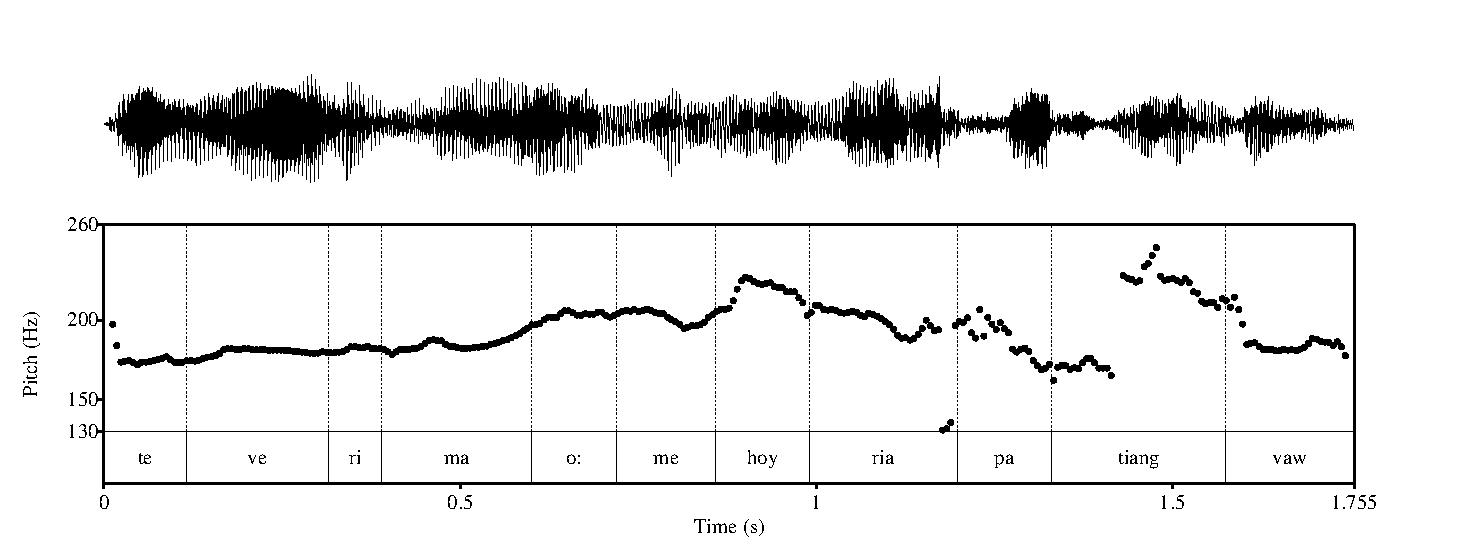
\includegraphics[width=1.0\textwidth]{figures/mehoy.eps} 
\caption{F$_0$ contour of example (\ref{mehoy})}\label{fig:ex1_pitch}
\end{center}
\end{figure}

\ea \label{mehoy}
\langinfo{Wooi}{Austronesian}{{\small MOB\_1\_EW 082}}\\
\glll teveri ma o: mehoy riapa tiang vaw\\
$<$i$>$taveri ma o: $<$i$>$mahoy $<$i$>$rapa tiang vaw\\
$<$3\textsc{sg}$>$return come \textsc{int} $<$3\textsc{sg}$>$sit $<$3\textsc{sg}$>$roast fish \textsc{det}:\textsc{pl}\\
\glt ‘He came back (and) sat (and) roasted the fish.’
\z

The challenge to traditional linguistic analysis is that such verb strings in many cases bear no clear signs of any grammatical relationship between the participating verbs. In the example, the verbs all appear to be of equal syntactic rank as no inflectional differences can be found\footnote{I disregard \textit{ma} here for the moment as there are particular problems associated with its analysis. It is one of three directional elements that occur in postverbal position, adding path semantics to motion event construals. For historical and paradigmatic reasons, I analyse \textit{ma} in \ili{Wooi} as a verb, even though it has lost its ability to inflect for subject indexing.}. Thus, at first inspection they may be labelled underspecified verb sequences as they appear to be different from the better known clause-linking types traditionally divided into coordination and subordination. The existence of such verb strings poses problems for linguistic theory. If multi-verb strings in one group of languages are mapped on units (for instance by means of translational equivalence) that in another group of languages contain only a single verb, then any traditional approach that derives syntactic units such as the clause from \emph{one} lexical head would be challenged. Or to put it another way, the one-verb-one-clause formula does apparently not qualify for all contexts in all languages \citep{foley1985clausehood}. What is more, in typical instances of clause linkage it is often clear that we are dealing with two or more individuable clauses (for instance because they receive different degrees of finite marking). Multi-verb strings, however, do not always show clear signs of clause boundaries, and so it might be suspected that, in some cases,  multi-verbal but mono-clausal structures are involved. For instance, a similar assumption is made in better known cases of secondary predicates, such as in \textit{Alice drank the coffee cold} where we would not want to claim that \textit{the coffee (is) cold} is a separate clause nested into a matrix clause \textit{Alice drank coffee}.

\section{Verb serialisation}

Some of these verb strings have stimulated a profound discussion under the heading of \emph{verb serialisation} in the last decades (important contributions include \citealt{sebba1987syntax}, \citealt{Durie1997}, \citealt{Aikhenvald2006}, \citealt{foley2010events}, \citealt{haspelmath2016serial}). Within the emerging field of serial verb analysis, some of the most basic linguistic concepts such as \emph{clause} and \emph{predicate} on the grammatical level, \emph{intonation unit} on the phonological level, and even the notoriously difficult notion of \emph{event} in the cognitive domain have since been tossed back and forth in the attempt at gaining access to the hidden mechanics of these structures. The fundamental idea lurking behind the upsurge of research into serial verb constructions (henceforth SVCs) was that if no direct evidence for the status and mutual relationship of the verbs could be found, indirect evidence might be mustered by observing boundary behaviour on different planes of linguistic segmentation (grammar, prosody, gesture, eventhood etc). 

Very broadly, we may characterise two strands of reasoning that delimit the outer poles of the discussion. The first approach sets out from the assumption that SVCs are in essence little different from homologous construction types in other languages, be it on the level of syntax or on the cognitive-conceptual level. Ambiguous though those structures may look on the surface, their hidden mechanics of combination in principle follow the same rules as more familiar clause-linking constructions. Analysis, then, boils down to what \citet{givon1991serial} has called the typology of cross-language coding variability. We may dub this the nothing-new approach. 

The second approach, on the other hand, treats verb serialisation as a phenomenon that is genuinely unique and not compatible with a multi-clausal analysis at all. For instance, \citet{foley1984functional} proposed a special nexus type in SVCs which they termed cosubordination: two constituents that are neither coordinated nor subordinated but do show signs of mutual dependency. The view that verb serialisation is a syntactic phenomenon of its own tallies with considerations on the level of event conceptualisation and reporting. Perhaps most famous in this regard is Givón's dispute with Pawley, who claimed that a serial verb language like the Papuan language Kalam differs from English in the kinds of events that can be expressed in a single clause \citep{Pawley1987, pawley2011event}. Constraints on event packaging may be interpreted as being associated with deeper cognitive processing, and this has been taken as evidence that serialisation patterns are indicative of a marked cleavage. While some languages  allow certain events to be conceptualised with single lexical items, others require (at least some) event construals to be composed of a set of lexical items (each denoting one particular sub-event in the overall event plot). Accordingly, we may dub this second view on serial verbs the all-new approach.

One of the concerns in the literature on serialisation has been the question of where to draw the boundary between SVCs and other types of (unmarked) verb combinations. While no definitive consensus has yet been reached, there is a set of construction types that appears to form the core of what is considered to constitute serialisation. Abstracting very roughly from the body of literature, constructions seem more likely to be analysed as SVCs if: (i) the verbs are dynamic rather than stative, (ii) intransitive verbs are unergative rather than unaccusative (but cp. positional verbs), (iii) the function of the `functor' verb is comparable with a function in other languages in which a lexical item from a different part of speech is employed (`functional equivalence', for instance in case-marking, directional, aspectual SVCs etc), and (iv) the verbs encode single path trajectories rather than multiple ones as is found with episodic verbs (see e.g. \citealt{pawley2011event} for discussion). 

\section{Multi-verb constructions}

Yet not all multi-verb strings have received this degree of attention. There are types of verb combinations that have been mostly excluded from consideration in the serialisation debate, a point touched upon by \citep{givon1991serial}. He pointed out that typically those constructions are omitted from discussion that in all languages are coded with more than one verb, most prominently various types of complement-taking constructions as well as constructions in which one of the constituents receives an adverbial interpretation. To this we may add instances of modal verb constructions, periphrastic causatives, unmarked relative clauses and the like, all of which may bear a resemblance to canonical serial verb constructions. This lack of interest is somewhat remarkable inasmuch as some of these constructions \emph{prima facie} receive formal coding (or better: non-coding) in some serial verb languages that seems rather identical to canonical serialisation coding. If verb serialisation is to become more than a mere ``pre-theoretical umbrella term" as \citet{zwicky1990we} put it, analyses would need to account for such cases of coding similarity, and explain on which grounds verb serialisation \textit{proper} is indeed a different kind of verb combining than, say, a paratactic perception complement construction (e.g., the 'I see you come' type). 

An alternative starting point, which I will argue for throughout this study, is to take into consideration a wider set of multi-verbal patterns, not just a subset of ``canonical" serial verbs that seem uncontroversial across the current linguistic discussion. An inclusive approach will allow the redrawing of the boundaries of verb combination types if necessary, rather than force the application of \textit{a priori} disqualification criteria, thereby risking the exclusion of related constructions from analysis altogether. This is one of the reasons why I will use the more neutral and inclusive term multi-verb construction (from here on abbreviated as MVC) rather than serial verb construction\footnote{A brief disclaimer on terminology is in order here. While the term SVC has been in use for several decades (ultimately dating back to \citealt{christaller1875}), and has up to now been elaborated with a wealth of definitions, the term MVC is quite new, and thus still largely undefined. Both terms are thus hard to compare. Throughout this book, I will use the traditional term SVC for any verb string that has been defined as such in the literature on verb serialisation, except for examples that have been collected as part of my dataset. All other multi-verb strings will be referred to as MVCs, that is, comprising both the data retrieved from the published sources and analysed in the subsequent chapters, as well as any other string that contains more than one verb and appears to be underspecified in the sense defined below, without necessarily showing all criteria of a SVC.}. I will motivate this decision, as well as give a working definition of what I assume MVCs to be, at the end of Chapter \ref{ch:theory}.

\section{Aim and scope of the study}

This study is intended to contribute to our understanding of MVCs by looking at two groups of languages in Eastern Indonesia (from here on EI): the Papuan languages of the Bird's Head area, Northern Halmahera as well as the Timor-Alor-Pantar group on the one hand, and the Austronesian languages spoken on Sulawesi, the islands of Nusa Tenggara, the Moluccas, and in Western Papua on the other. The sample consists of an overall 32 languages made up of 16 Austronesian languages, and 16 non-Austronesian or Papuan languages. Figure \ref{map:overview} provides a first overview of the area as well as the languages chosen to be included in the sample.

\begin{sidewaysfigure}
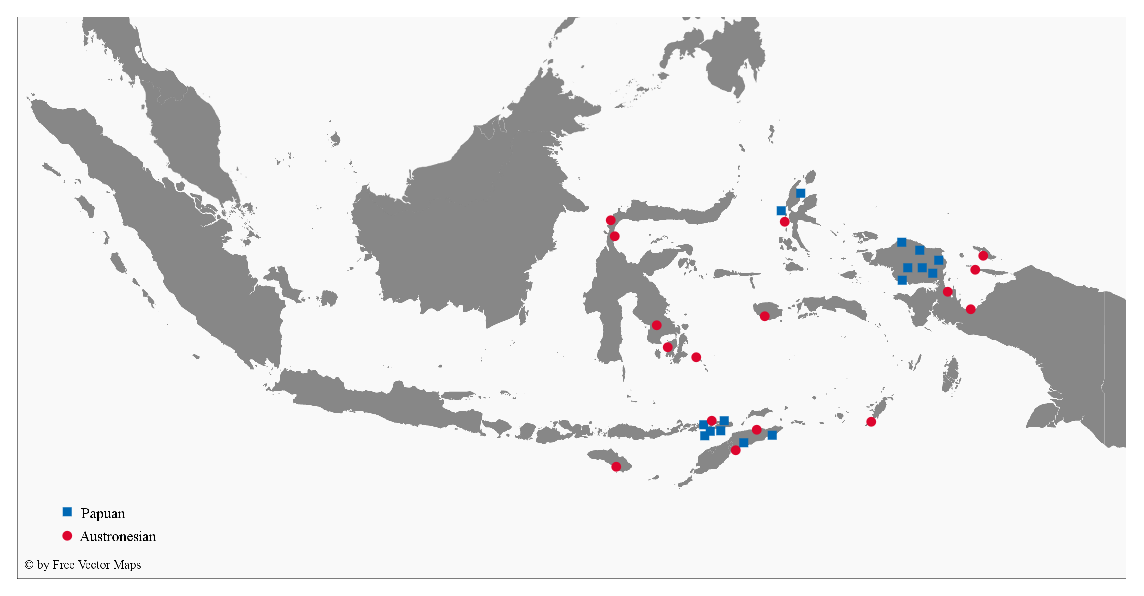
\includegraphics[width=\columnwidth]{figures/Map_overview_klein.eps}
\caption[Geographical distribution of sample languages]{Geographical distribution of the sample languages across Eastern Indonesia. Languages are grouped into Austronesian (red circles) and Papuan (blue squares).}\label{map:overview}
\end{sidewaysfigure}

The data for this work has been collected from published grammars, research papers as well as from two extensive language documentation corpora, and is introduced in §\ref{sec:data} below. In the course of this study, I will collate and discuss the grammatical (Chapter \ref{ch:gram}) and semantic (Chapter \ref{ch:sem}) properties of multi-verb strings in these languages. The results obtained from these sections will then in Chapter \ref{ch:constructions} feed into a typology of MVCs. 

My analysis of MVCs from the EI region is primarily informed by the following hypotheses that I will flesh out in the chapters to come:

\begin{footnotesize}
\begin{itemize}
\item \textbf{\#Hypothesis 1:} Although the morphosyntactic make-up of MVCs in EI is remarkably similar across different construction types, these MVCs are constructed through different techniques (mentioned below in \#H2)
\item \textbf{\#Hypothesis 2:} Verbal interaction in MVC formation involves three principle techniques at the clausal level: merging (of features), modification and staging (alignment of spatiotemporally distinct stages)
\item \textbf{\#Hypothesis 3:} The different techniques of MVC formation are based on a layered structure of event conception, each technique being associated with a particular level of the event schema
\item \textbf{\#Hypothesis 4:} Some MVC types may be embedded into a constructional slot of another MVC resulting in stacked MVCs
\item \textbf{\#Hypothesis 5:} Not all EI languages use all techniques. Differences in the use of MVC patterns indicate different linguistic subareas or diffusion zones of grammatical traits. MVC use radiates out from two hotspots of MVC innovation: the Timor-Alor-Pantar and the Bird's Head region, respectively.
\end{itemize}
\end{footnotesize}

One of the goals of this work is to put together form and meaning, and explore the ways in which the languages of the sample mould the different semantic combinations into grammatical form. I will try to show that some form-function mappings are predominant in the dataset although formal encoding of MVCs in general does not immediately mirror the semantic relationship between their verbs. What is more, I will argue throughout this book that the fact that such verb strings are formally underspecified does not necessarily mean that all instances belong to the same string type nor that we invariably deal with flat concatenations of verbs. The analysis proposed in the next chapters rather rests upon the claim that some combination types in fact host embedded MVCs and are better analysed as (covert) hierarchical structures (a concept that I will metaphorically refer to as \isi{stacked MVC}s).

A second main concern of this work is to explore the numerous treatments of serial verbs and related constructions in the languages of Eastern Indonesia. While typological research into serial verbs has been done for the Oceanic languages with considerable detail \citep{crowley2002serial, bril2004complex, bril2007nexus}, comparative analyses of Eastern Indonesian languages are still rare and largely confined to the exploratory study of \citet{vanstaden2008serial}. This book is the first attempt to explore the use of MVCs throughout all of Eastern Indonesia, including peripheral parts such as Sulawesi, by taking into account a comprehensive dataset of both published data and data from extensive language documentation corpora. To my knowledge, this book represents the first research into the areal characteristics of multi-verb strings that is explicitly based on a thorough assessment of the defining properties of both SVCs and MVCs. The findings arising from this assessment will be shown to support the assumption that Eastern Indonesia constitues a Sprachbund area.

SVCs have been reported for most of the languages in Eastern Indonesia on which data are available, displaying an intriguing range of verb combinations. Some grammars allot much space to the description of SVCs, while others note their presence in passing. The heterogeneous distribution of information as well as the different theoretical underpinnings of these analyses renders such a comparative task a challenging yet also rewarding endeavour. I hope that by evaluating this wealth of constructions this work may contribute another piece to the jigsaw of finding commonalities in the diversity of verb combination patterns.

The remainder of this chapter serves as a first introduction to the phenomenon under investigation, as well as to the data set on which it is based. The next section will illustrate basic properties of underspecified verb sequences and highlight some of the analytical problems. The chapter ends with a presentation of the data sample, its various sources, and a brief discussion of the methodology used throughout the study.

\section{Underspecified verb sequences}

At the beginning of this chapter, I described serial verb structures in broad terms as underspecified verb sequences. What does underspecified mean? Underspecified in my sense refers to a lack of overt signals: Verbs in SVCs do not normally bear formal marks of dependency that would enable us to identify the kind of relationship holding between them. Infinitive morphology, non-finite verb forms, reduced verbal inflection, as for instance with medial verbs or converbs -- all such devices are typically not found in SVCs, so that potential hierarchical relationships between the verbal constituents are not cued directly. In fact, it appears that we do not even know whether there is a particular grammatical relationship present between the verbs, or whether the verbs are placed next to each other in loose apposition. If this turned out to be true, we might better understand the verbs as put together only on the output level of prosodic segmentation rather than on the syntactic level of constituent structure, in much the same way as, say, a phonological word may string together constituents that, from a grammatical perspective, constitute independent units. This idea is not at all implausible as natural speech data show, and I will return to this issue briefly in Chapter \ref{ch:discussion}. 

For now, suffice it to say that underspecified means here that verbs in serial verb languages typically are not grammaticalised with regard to being capable of expressing different degrees of finiteness. This does not mean that verbs in these languages do not inflect for verbal categories such as person marking or TAM categories. They may do so, and in fact most languages in the EI data set inflect for one category or another. The crucial point is that verbal inflection in most of these languages is not structurally exploited in such a way as to systematically encode differences in verbal hierarchy\footnote{While this seems to hold for most of the languages I have looked at, there are notable exceptions where languages do provide finiteness options to mark off certain construction types. In the Papuan language \ili{Yimas}, for instance, simultaneous events have to be marked by a non-finite oblique case-marking nominalization \citep[142]{foley2008}, whereas sequential event chains may be encoded by SVCs.}. At least in the languages of Eastern Indonesia, presence or absence of inflection is governed by phonological rules or membership to a certain verb class rather than by restrictions imposed by SVCs.

Let us now turn to some examples. The examples below are chosen to illustrate the most frequent formal and semantic characteristics of SVCs in the literature. They are taken from the major linguistic areas for which serialisation has been reported: West Africa, China, and also Papua (see \citealt[2]{senft2008intro}), are the areas where early language descriptions first spotted serialised verb patterns \citep{sebba1987syntax, Matthews2006}. \citet{christaller1875} with his account of the Twi language (\ili{Akan}), spoken in Ghana, is usually credited with being the first explicit description of serial verb constructions. The linguistic discussion of serialisation later spread to creole languages (starting with Atlantic Creoles, later followed by Pacific and South Asian Creoles, see \citealt{nordhoff2012}), and later again to Papuan and Austronesian languages in the Pacific area, mainland South-East Asia and South America \citep{senft2008event}. Linguistic descriptions of SVCs from these areas have all contributed greatly to our understanding of verb combination types, and some of the defining features of SVCs occur over and over again\footnote{Note that many of these examples contain free translations that seem somewhat confusing to scholars beginning to study SVCs. In order to render the meaning of SVCs into well-formed English, conjunctions are often inserted into translations. Conjunctions (and other material) in brackets should therefore not be taken literally but understood as stylistic means to facilitate understanding. The same goes for conjunctions that are not in brackets but do not have a corresponding morpheme in the transcription tier: I have refrained from altering the free translation of examples where the author did not indicate stylistic additions so as to not violate the utterance meaning, or to hamper alternative analyses on the reader's part.}.

\ea
West Africa\\
\ea \label{Twi01}
\langinfo{\ili{Akan} (Twi)}{Niger-Congo}{\citealt{christaller1875}, quoted in \citealt[21]{ameka2005multiverb}}\\
\gll Y\textipa{E}-\textbf{s\textipa{O}re}-e nt\textipa{\'E}m \textbf{k\textipa{O}}-\textipa{O}  fie\\
\textsc{1}\textsc{pl}-rise-\textsc{pst} quickly go-\textsc{pst} home\\
\glt ‘We arose [got up, F.K. Ameka] quickly (and) went home’
\ex \label{Ewe01}
\langinfo{\ili{Ewe}}{Niger-Congo}{\citealt[135]{ameka2006ewe}}\\
\gll e-\textbf{k\textipa{\'o}} fi\textipa{\'a} k\textipa{\'o} \textbf{dz\textipa{\'a}} ati-a \\
\textsc{3}\textsc{sg}-raise axe take hack stick-\textsc{def}\\
\glt ‘He used an axe and hacked the wood’
\z
\z

\ea
Sinitic languages\\
\ea \label{Man01}
\langinfo{\ili{Mandarin}}{Sino-Tibetan}{\citealt[96]{LiThompson1973}}\\
\gll Zh\textipa{\=a}ng-s\textipa{\=a}n \textbf{chu\textipa{\=a}n-shang} y\textipa{\=i}fu \textbf{ti\textipa{\`a}o} zai d\textipa{\`i}-shang\\
Zhang-san put-on clothes jump on floor\\
\glt ‘Zhang-san put on his clothes and then jumped on the floor’
\ex \label{Can01}
\langinfo{\ili{Cantonese}}{Sino-Tibetan}{\citealt{omelia1966first}, quoted in \citealt[69]{Matthews2006}}\\
\gll keoi$^5$ \textbf{jap$^6$} \textbf{heoi$^3$} \textbf{co$^5$}\\
\textsc{3}\textsc{sg} enter come sit\\
\glt ‘He went in and sat down’
\ex \label{Can02}
\langinfo{\ili{Cantonese}}{Sino-Tibetan}{\citealt[75]{Matthews2006}}\\
\gll keoi$^2$ \textbf{haam$^3$}-\textbf{sap$^1$}-zo$^2$ go zam$^2$tau$^4$\\
\textsc{clf} cry-wet-\textsc{prfv} \textsc{clf} pillow\\
\glt ‘She's made her pillow wet by crying’
\z
\z

\ea
creole languages\\
\ea \label{Sra01}
\langinfo{\ili{Sranan}}{English based Creole, Atlantic}{\citealt[50]{sebba1987syntax}}\\
\gll Kownu \textbf{seni} wan boskopu \textbf{gi} tigri\\
King send a message give tiger\\
\glt ‘King sent Tiger a message/a message to Tiger’
\ex \label{Sra02}
\langinfo{\ili{Sranan}}{English based Creole, Atlantic}{\citealt[40]{sebba1987syntax}}\\
\gll \textbf{lon} \textbf{go} \textbf{teki} a buku \textbf{tyari} \textbf{go} \textbf{gi} a leriman\\
run go take the book carry go give the teacher\\
\glt ‘Run and fetch the book and take it to the teacher’
\z
\z

\ea
Papuan region\\
\ea \label{Ala01}
\langinfo{\ili{Alamblak}}{Sepik}{\citealt[20]{bruce1988}}\\
\gll wa-ha-\textbf{muh}-\textbf{h\textipa{\textbari}ta}-ta\textipa{\~n}-\textipa{\~n}-m-ko\\
\textsc{imp}-\textsc{caus}-climb-put-\textsc{comp}-\textsc{2}\textsc{sg}-\textsc{3}\textsc{pl}-up\\
\glt ‘Lift them up (and) leave them up here’
\ex \label{Ala02}
\langinfo{\ili{Alamblak}}{Sepik}{\citealt[20]{bruce1988}}\\
\gll \textbf{tat}-\textbf{noh}-m\textipa{\"e}-an-r\\
hit-die-\textsc{rpst}-\textsc{1}\textsc{sg}-\textsc{3}\textsc{sg}.\textsc{m}\\
\glt ‘I killed him by hitting (him)’
\ex \label{Yim01}
\langinfo{\ili{Yimas}}{Ramu-Lower Sepik}{\citealt[80]{foley2010events}}\\
\gll arm-n kay i-ka-\textbf{ak}-mpi-\textbf{wul}\\
water-\textsc{obl} canoe.\textsc{viiisg} \textsc{viiisg}.\textsc{obj}-\textsc{1}\textsc{sg}.\textsc{act}-push-\textsc{seq}-put.in\\
\glt ‘I pushed the canoe down into the water.’
\z
\z

\ea
Oceanic region\\
\ea \label{Paa01}
\langinfo{Paamese}{Austronesian}{\citealt[55]{crowley2002serial}}\\
\glll inau \textbf{nuas} vuas \textbf{he:mat} \\
inau ni-uasi vuasi hee-mate\\
\textsc{1}\textsc{sg} \textsc{1}\textsc{sg}.\textsc{dist}.\textsc{fut}-hit pig \textsc{3}\textsc{sg}.\textsc{dist}.\textsc{fut}-die\\
\glt ‘I will hit the pig to death.’
\ex \label{Paa02}
\langinfo{Paamese}{Austronesian}{\citealt[60]{crowley2002serial}}\\
\glll i:r \textbf{reheso:n} vakili \textbf{he:ha}\\
iire rehe-sooni vakilii hee-haa\\
\textsc{1}\textsc{pl}.\textsc{in} \textsc{1}\textsc{pl}.\textsc{in}.\textsc{dist}.\textsc{fut}-throw canoe \textsc{3}\textsc{sg}.\textsc{dist}.\textsc{fut}-go\\
\glt ‘We will throw the canoe away.’
\z
\z

If we just compare the visible surface features of these constructions, we see both variation between languages and shared feature values. On the level of constituent order, the serial verbs may either form a coherent group (ex. (\ref{Can01}), (\ref{Can02}), (\ref{Sra01}), (\ref{Ala01}), (\ref{Ala02}), (\ref{Yim01})), or their sequence may be broken up by other constituents (ex. (\ref{Twi01}), (\ref{Ewe01}), (\ref{Man01}), (\ref{Sra01}), (\ref{Sra02}), (\ref{Paa01}), (\ref{Paa02})). If the first verb is transitive and the direct object is overtly expressed, the argument may either stand right after the verb (ex. (\ref{Ewe01}), (\ref{Man01}), (\ref{Sra01}), (\ref{Sra02}), (\ref{Paa01}), (\ref{Paa02})), or the verbs may form a tight unit with the object in preverbal position or after the last verb in the series (ex. (\ref{Can02}), (\ref{Yim01})). Yet even if the first verb is intransitive, the construction may still permit the insertion of a modifier (as the adverb \textit{nt\textipa{\'E}m} in the \ili{Akan} example shows). 

Another criterion that shows variation is word boundaries: a sequence of serial verbs may either form one phonological word, or each verb may constitute an independent word. Many Papuan languages combine verbal roots on the morphological level, but example (\ref{Can02}) shows that the phenomenon may also occur in other areas. If the verbs come to stand within one phonological word, it may be difficult to distinguish serialisation (which started its linguistic career essentially as a syntactic phenomenon) from verbal compounds (see e.g. \citealt{vanstaden2008serial} for discussion). Some writers like \citet{devries2004} have argued that stress assigment is an indicator of whether a multi-verbal root structure constitutes a compound (one stress peak) or a phrasal construction (stress peak on each root). \citet{vanstaden2008serial} explicitly exclude root combinations with only one primary accent from the group of serial verb constructions in spite of striking semantic similarities. \ili{Inanwatan} for instance has no serial verbs, according to their analysis, but only verbal compounds. In this study, I will take a more liberal stance on these structures and will subsume both under the heading of multi-verb construction, for the following reasons: First, stress assignment in multi-root structures is not always clear from the data sources. Second, it has been claimed that serial verb structures may evolve into compounds at some point (see \citealt[27]{vanstaden2008serial}) and so we might expect \isi{serialisation} structures and \isi{compound}s to be conceptually similar. And third, some compounds fit into semantic types that are otherwise observed in serial verbs, so that it seems more interesting not to exclude such cases at this point. 

The main weakness of the stress test is the presupposition that the language in question does have a word-level prosodic system that enables the distinction between verbal compounds and (word-level) serialisation. In general, the presence or absence of features used to confirm the existence of SVCs indeed poses a well-known problem. Not all languages show all features. This is pointed out by \citet[22]{vanstaden2008serial}: 

\begin{quote}What often obscures the discussion on serial verb constructions is [...] that criteria that can be applied in one language to distinguish, for instance, SVCs from subordination or compounding, simply may not be applicable for other languages.\end{quote}

For instance, if we compare the inflection marks on the verbs above, we are \textit{prima facie} not able to define a clear \textit{tertium comparationis}: some of the languages show person marking on the verbs (\ili{Ewe}, \ili{Yimas}), others (may) mark TAM values (\ili{Mandarin}, \ili{Cantonese}), and still others have both (\ili{Akan}, \ili{Alamblak}, \ili{Paamese}) or no inflectional marking at all (\ili{Sranan}). Presence or absence of verbal morphology is often used to infer a hierarchical status of the constituent, and inflected verbs may be analysed as being head of a specific construction. A difference in verbal inflection between the verbs in a SVC could therefore be taken as evidence that the uninflected verb is of a lower rank than the inflected (matrix) verb. The \ili{Akan} and \ili{Ewe} examples above could be interpreted in such a way. 

A related factor that might also indicate differences in verbal rank is the overt expressability of arguments in a SVC. In the \ili{Cantonese} and \ili{Paamese} examples we see that the subject argument is only expressed once as a pronoun before the first verb, as the second verb does not trigger the use of a subject pronoun. While pronoun assignment may in general be governed by more general pragmatic factors in pro-drop languages, the \ili{Paamese} data show that there are hidden restrictions at work in particular constructions. \citet{crowley2002serial} observes that in examples such as (\ref{Paa01}) overt expression of the second subject (which is co-referential with the object of the first verb) is not licit. If an independent pronoun is inserted into the preverbal subject slot of the second verb, the construction apparently changes with regard to two properties: (i) the interpretation of the event becomes sequential ('hit the pig and it will die' instead of 'hit the pig to death'), and (ii) it becomes possible to insert the coordinator \textit{kaa} 'and' between the verbal constituents without any clear change in meaning. This is evidence that in \ili{Paamese} switch subject constructions the second verb has a deranked status and does not show full independence with regard to subject assignment.

Summing up this brief analysis of the examples, we have seen that there are several parameters with different possible values in SVC formation, for instance verbal inflection patterns, constituent placement and argument realisation. The same amount of variation is found in the semantics of the verb combinations. \citet{givon1991serial} classified SVCs into five distinct functional types:

\begin{footnotesize}
\begin{itemize}
\item \textbf{Case-role marking}: a functor verb is grammaticalized into a verbal case marker of different sorts of core or oblique arguments, for instance patient, benefactive, instrumental, or locative
\item \textbf{Co-lexicalization}: two verbs are co-lexicalized and form a more complex verbal concept
\item \textbf{Deictic-directional marking}: deictic directional verbs like `come' or `go' lend their deictic meaning to other verbs of motion or transport creating complex deictic expressions of motion in space
\item \textbf{Tense-aspect marking}: a functor verb is grammaticalized into a marker of aspectual or modal function
\item \textbf{Evidentiality and epistemic marking}: a functor verb has acquired a reading of evidentiality
\end{itemize}
\end{footnotesize}

Of these broad functions, case-role marking, co-lexicalisation, deictic-directional marking, and, to a lesser extent, tense-aspect marking can also be found in the languages of Eastern Indonesia. Example (\ref{Ewe01}) is a good instance of the case-role marking type: the argument \textit{fi\textipa{\'a}} 'axe' is introduced as a theme argument by the first verb \textit{e-\textbf{k\textipa{\'o}}} 'raise/take'. At the same time, one can argue that, within the particular context of the construction, it also serves as the instrument to the action of hacking, and thus \textit{e-\textbf{k\textipa{\'o}}} might be analysed as a grammaticalised verbal instrument marker. The co-lexicalisation scenario can possibly be observed in the second \ili{Cantonese} example (\ref{Can02}).

Yet with all this variation in place, SVCs do show signs of similar overall construal. There are no morphological cues to differences in verbal hierarchy (other than differences in verbal inflection). There are no connectors, conjunctions, complementisers or other formatives between the verbs (\ili{Yimas} \textit{-mpi-} provides an exception here). TAM values (e.g. the past marker \textit{-e/-\textipa{O}} in (\ref{Twi01}) or the remote past marker \textit{-m\textipa{\"e}} in (\ref{Ala02})) or markers of illocutionary force (as imperative \textit{wa-} in (\ref{Ala01})) are canonically interpreted as having scope over the entire construction. All verbs share at least one of their arguments with each other. And for many languages, SVCs have been reported to occur under a coherent intonation contour, suggesting that on the prosodic level the verbs are grouped into one homogeneous unit.

The features presented in this brief preview will be taken up again in the following chapters, and will be critically examined as to whether or not they may be applied to the EI dataset. In Chapter \ref{ch:theory}, an analysis of the defining properties of serial-verb constructions is laid out. We shall see that not all features are equally useful, or can be applied without resorting to further properties that, from language to language, may be quite different. While I will eventually single out three morphosyntactic properties that are put to the test in Chapter \ref{ch:gram}, the results  show, I will argue, that looking at morphosyntactic properties alone will not give rise to any meaningful analysis. In Chapter \ref{ch:sem}, the analysis will therefore shift to a semantic approach, identifying four underlying techniques of MVC formation on different conceptual levels. It is these semantic techniques that will then in Chapter \ref{ch:constructions} feed into a typology of MVCs. Quite unlike Givón's functional typology of SVCs from above, we will arrive at four constructional families that each accomodate a set of constructions in use across most of EI.

In the next section I turn to my area of research and briefly introduce the dataset on which this study is based.

\section{Data sample and methodology}\label{sec:data}

As already mentioned, this study was primarily designed as a literature survey in order to gather data on serial verb constructions in the area of Eastern Indonesia that would otherwise remain ``tucked away" in grammars and research papers. By collating data from different EI languages, both Austronesian and Papuan, I hope to explore the wealth of construction types, their distribution and distinct properties in this area. To this end, I identified 30 languages for which sufficient published data were available. This set of published data was further complemented with another two languages for which extensive language documentation corpora were available: \ili{Waima'a} and \ili{Wooi}. Both languages had been investigated in DoBeS language documentation projects (I was part of the Wooi project) and I had sufficient working experience with them. 

The languages for the literature survey were chosen to meet the following conditions:

\begin{footnotesize}
\begin{itemize}
\item Enough material for at least 25 data points from a range of different constructions\footnote{Except, of course, for EI languages that only make very limited use of serial verbs, or do not use them in the first place. All languages reviewed for the dataset turned out to use at least some MVCs, so that all languages can be said to meet this condition. Only Austronesian \ili{Selaru}, spoken in the southern Moluccas, appears to have developed a small set of linking elements that are extensively used throughout what otherwise looks just like ordinary MVCs.}
\item A grammatical description dealing with SVCs and their language-specific properties
\item Sufficient geographical and genetic variation within the dataset to model all subareas and taxa
\item Recent publications
\end{itemize}
\end{footnotesize}

Table \ref{table:sample} below gives an overview of the languages that were included in the dataset on these grounds. The first goal, at least 25 (varied) data points, was easy to achieve as most book-length publications included numerous varied examples for SVCs. The normal form for grammars to deal with the topic is to devote an exclusive chapter or section to the discussion of serial verbs. Therefore, the second requirement was also met by almost all data sources. Very few publications deviated from this pattern, but were included nonetheless: The grammars on \ili{Abun} \citep{berry1999} and \ili{Makalero} \citep{huber2011} do not directly discuss serial verbs, nor does the sketch grammar on \ili{Dusner} \citep{dalrymple2012}. They were included as they displayed many serial verb constructions among their examples in other sections. The \ili{Mor} data paper \citep{kamholz2009} is another exception, since it does not contain any grammatical description but only an interlinearized text and a dictionary. As an outlier to both the Bird's Head area as well as to the South Halmahera-West New Guinea taxon, I decided to include \ili{Mor} nonetheless, treating it as if the data were taken from a language documentation corpus like the ones for \ili{Waima'a} and \ili{Wooi}.

The third goal was to include as many sub-branches of the language families as possible, and to attain a geographical distribution of the sample languages that would cover different subareas in EI. To this end, I tentatively assumed four subareas for which rather homogeneous MVC features might be expected: Sulawesi and Western (Bird's Head) Papua were chosen as subareas because of their geographical coherence and their linguistic profile, with the former showing most western Austronesian features, and the latter displaying the central diffusion zone of (West) Papuan features into adjacent Austronesian languages. Two further subareas have been defined in central Wallacea: Nusa Tenggara comprises the lesser Sunda Islands from Flores in the west up to the Timor achipelago including Alor and Pantar. Finally, Maluku comprises the area from the Aru Islands in the south, across Banda and Seram and up to the Halmahera archipelago in the north. A subdivision of Eastern Indonesia into these four subareas is also supported by findings from biogeographical dispersal barriers through the region. The borders of the subareas match with the biological demarcation lines briefly outlined in §\ref{sec:area_intro} (cf. Figure \ref{map:wallacea} for an overview)\footnote{The only exception to this is the border between the subareas of Nusa Tenggara and Maluku. Following Zollinger's Line would require the inclusion of \ili{Selaru} into the Nusa Tenggara group (see Figure \ref{map:wallacea}). As Selaru appears to share more characteristics with \ili{Buru} than with Austronesian languages spoken on Timor, I rather placed \ili{Selaru} with the languages of the Maluku group.}. Figure \ref{map:subareas} illustrates the four subareas and their associated languages. %Note that, throughout this study, an abbreviation referring to the respective subarea is placed next to the language name in each example: \textsc{\acs{sul}}, \textsc{\acs{nus}}, \textsc{\acs{mal}}, or \textsc{\acs{pap}}.

\begin{sidewaysfigure}
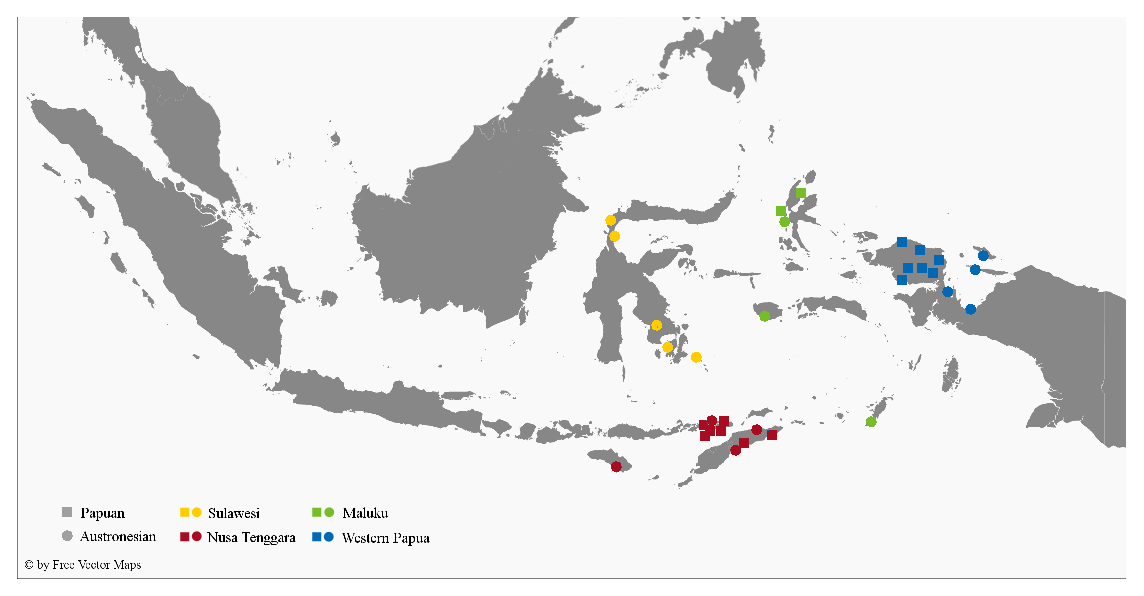
\includegraphics[width=\columnwidth]{figures/Map_overview_klein_subareas.eps}
\caption[Geographical distribution of the sample languages across subareas]{Geographical distribution of the sample languages across the four subareas Sulawesi, Nusa Tenggara, Maluku, and Western Papua. Languages included in the sample are given in coloured squares (Papuan) and circles (Austronesian).}\label{map:subareas}
\end{sidewaysfigure}

As can be seen from Table \ref{table:sample}, the number of sample languages in the different subareas is not as balanced as I hoped. For both Western Papua and Nusa Tenggara there were a lot of recent grammars available, especially for the Papuan languages of the Bird's Head and the Timor-Alor-Pantar area, both of which have attracted much attention throughout the last decades. Sulawesi is also covered by some excellent grammars though the area that is probably most interesting to a survey on serial verbs is the transition area in south-east Sulawesi, for which only \ili{Muna} \citep{vandenberg1989} and \ili{Tukang Besi} \citep{donohue1999} have received full-fledged grammatical descriptions so far. Another lesser studied area in terms of published grammars seems to be the Maluku region. As a result, both the Maluku area and Sulawesi remain underrepresented in my sample, while the TAP area and the Bird's Head contributed most languages (and data points).

\begin{table}[!tbp]
\begin{center}
\begin{scriptsize}
\begin{tabular}{>{\footnotesize}l >{\footnotesize}l >{\scriptsize}p{3.2cm} >{\scriptsize}l r r r}
\hline\hline
\multicolumn{1}{l}{group} & 
\multicolumn{1}{l}{language } & 
\multicolumn{1}{l}{source} & 
\multicolumn{1}{l}{type} & 
\multicolumn{3}{c}{data points}\tabularnewline
\multicolumn{1}{l}{} & 
\multicolumn{1}{l}{} & 
\multicolumn{1}{l}{} & 
\multicolumn{1}{l}{} &
\multicolumn{1}{c}{ex} & 
\multicolumn{1}{c}{grm} & 
\multicolumn{1}{c}{txt}\tabularnewline
\hline
\multirow{5}{*}{\rotatebox[origin=c]{90}{Sulawesi}}
&\ili{Muna}&\citealt{vandenberg1989}&grammar&$  0$&$ 39$&$ 11$\tabularnewline
&\ili{Pendau}&\citealt{Quick2007}&grammar&$  0$&$ 51$&$  0$\tabularnewline
&\ili{Tajio}&\citealt{mayani2013grammar}&grammar&$  0$&$ 27$&$  5$\tabularnewline
&\ili{Tolaki}&\citealt{mead2008verb}&article&$  0$&$ 65$&$  0$\tabularnewline
&\ili{Tukang Besi}&\citealt{donohue1999}&grammar&$  0$&$ 48$&$ 22$\tabularnewline
\hline
\multirow{11}{*}{\rotatebox[origin=c]{90}{Nusa Tenggara}}
&\ili{Abui}&\citealt{kratochvil2007grammar}&grammar&$  0$&$109$&$  0$\tabularnewline
&\ili{Alorese}&\citealt{klamer2011alorese}&sketch grammar&$ 21$&$ 11$&$ 15$\tabularnewline
&\ili{Bunaq}&\citealt{schapper2009bunaq}&grammar&$  0$&$ 87$&$  0$\tabularnewline
&\ili{Kaera}&\citealt{klamer2014kaera}&sketch grammar&$  8$&$ 16$&$  0$\tabularnewline
&\ili{Kambera}&\citealt{klamer1998grammar}&grammar&$ 6$&$ 32$&$  6$\tabularnewline
&\ili{Klon}&\citealt{baird2008grammar}&grammar&$ 43$&$ 57$&$  0$\tabularnewline
&\ili{Makalero}&\citealt{huber2011}&grammar&$76$&$  0$&$  0$\tabularnewline
&\ili{Teiwa}&\citealt{klamer2010grammar}&grammar&$  2$&$ 74$&$  9$\tabularnewline
&\ili{Tetun Fehan}&\citealt{vanklinken1999grammar}&grammar&$  7$&$ 66$&$  0$\tabularnewline
&\ili{Waima'a}&\citealt{belo2002-2006}&corpus&$  0$&$  0$&$176$\tabularnewline
&\ili{Western Pantar}&\citealt{holton2014western}&sketch grammar&$  4$&$ 34$&$  0$\tabularnewline
\hline
\multirow{5}{*}{\rotatebox[origin=c]{90}{Maluku}}
&\ili{Buru}&\citealt{grimes1991buru}&grammar&$ 10$&$ 55$&$ 3$\tabularnewline
&\ili{Selaru}&\citealt{coward2005}&grammar&$ 13$&$  0$&$ 12$\tabularnewline
&\ili{Taba}&\citealt{bowden2001taba}&grammar&$  0$&$ 32$&$ 12$\tabularnewline
&\ili{Tidore}&\citealt{vanstaden2000tidore}&grammar&$  54$&$ 12$&$ 26$\tabularnewline
&\ili{Tobelo}&\citealt{holton2003tobelo}&sketch grammar&$ 31$&$ 7$&$ 6$\tabularnewline
\hline
\multirow{11}{*}{\rotatebox[origin=c]{90}{Western Papua}}
&\ili{Abun}&\citealt{berry1999}&grammar&$ 33$&$  0$&$  0$\tabularnewline
&\ili{Biak}&\citealt{vanheuvel2006}; \citealt{mofu2008biak}&grammar&$ 33$&$ 17$&$ 17$\tabularnewline
&\ili{Dusner}&\citealt{dalrymple2012}&sketch grammar&$ 33$&$  0$&$ 16$\tabularnewline
&\ili{Hatam}&\citealt{reesink1999grammar}&grammar&$  0$&$ 49$&$  0$\tabularnewline
&\ili{Inanwatan}&\citealt{devries2004}&grammar&$ 14$&$  4$&$ 10$\tabularnewline
&\ili{Maybrat}&\citealt{dol2007grammar}&grammar&$ 28$&$ 50$&$  0$\tabularnewline
&\ili{Mor}&\citealt{kamholz2009}&paper (text\&dict)&$  0$&$  0$&$ 71$\tabularnewline
&\ili{Moskona}&\citealt{gravelle2010grammar}&grammar&$  0$&$ 79$&$  0$\tabularnewline
&\ili{Mpur}&\citealt{ode2002sketch}&sketch grammar&$ 11$&$  7$&$ 44$\tabularnewline
&\ili{Sougb}&\citealt{reesink2002grammar}&sketch grammar&$ 20$&$  7$&$  13$\tabularnewline
&\ili{Wooi}&\citealt{kirihio2009dobes}&corpus&$  0$&$  0$&$190$\tabularnewline
\hline
Subtotal& & & &$ 447$&$ 1035$&$ 664$\tabularnewline
Total&$ 32$& & & & & $ 2146$\tabularnewline
\hline
\end{tabular}
\caption[Overview of the EI dataset]{Overview of the languages and the different types of data used. Further explanation in the prose.}
\label{table:sample}
\end{scriptsize}
\end{center}
\end{table}

If data points of MVCs were only collated from the chapters and sections specifically devoted to them, one could wonder whether the sample of construction types is indeed representative for the language or whether the author was in some sense biased. Such a bias could for instance arise because a certain class of constructions attracted specific attention in the literature at that time, or because the author was intrigued by some unusual property. I tried to account for this potential bias by also browsing through other chapters/sections of the respective publication and noting down MVCs from examples meant to explain quite different things. Occurrences of MVCs in unrelated examples also proved that MVCs in those language were not uncommon at all. Accordingly, I differentiated between data points from SVC discussions (\textit{grm} in Table \ref{table:sample}) and data points from unrelated chapters/sections (which I counted as \textit{ex}). In cases where I felt that I did not have enough data points at hand or where the construction types seemed not to reflect the total breadth of MVCs in a language, I also collected further examples from appended interlinearised texts (where available). These data points were glossed as \textit{txt}. The two language documentation corpora, \ili{Waima'a} and \ili{Wooi}, served as further data sources for the two subareas Nusa Tenggara and Western Papua. All in all, I gathered 2146 examples of MVCs from 32 languages in EI.

In the next chapter I turn to the Eastern Indonesian region. I will show that a linguistic definition of Eastern Indonesia can be based on typological and genetic grounds, and that this definition aligns well with both biological and geographical patterns. I will first introduce the region as a linguistic area, followed by an introduction to the languages that make up the sample upon which this work is based. As a basic understanding of the EI languages as well as of the literature on serialisation is required in order to interpret the dataset, I defer a more thorough discussion of how I collated the EI data to the end of Chapter \ref{ch:theory}.
\chapter{The Eastern Indonesian linguistic area}\label{ch:area}

\section{Introduction} \label{sec:area_intro}
Indonesia is one of the linguistically most diverse countries of the world and hosts about 700 languages spread across a vast archipelago with thousands of islands. Stretching from the large islands of Sumatra and Borneo in the far west, along the chains of the Sunda-Banda arc system, up to the western part of mainland New Guinea in the east, the territory of today's Indonesia has provided space for a multitude of ethnic groups to evolve and develop a wealth of distinct cultural and linguistic systems. Archaeologists, geneticists, and linguists have all contributed evidence that there were several major waves of human migration spreading over the area. The first humans migrating into the archipelago and beyond set forth as early as about 50,000 BCE in the Late Pleistocene \citep{capelli2001}, at a time when Australia, New Guinea and parts of Indonesia were still connected, and formed the prehistoric continent Sahul. These groups eventually reached New Guinea and continued further eastward to the Solomon Islands and southward into Australia. The descendants of these migrants are associated with the ethnic groups of Aborigines in Australia and the Papuans that live on the island of New Guinea as well as in its vicinity. 

The last wave of migrants arrived much later in the Indonesian area, dating back to a time frame around 4,500 BCE \citep{Bellwood1998, Bellwood2007}. These groups were the ancestors of the Austronesian people. They probably originated from South China, migrated further to the island of Taiwan, and from there on followed along the Philippine Islands down southwards \citep{Tryon1995, capelli2001}. In the course of their dispersal into the Malay archipelago, their languages eventually replaced the Pre-Austronesian languages, or drove them into the interior parts of the islands. Archaeological evidence suggests that the situation was by no means the same across the Indonesian archipelago. While the western islands of Indonesia had only small Pre-Austronesian populations along the coastlines, which must have entered into a serious competition with the Austronesian seafaring people, the opposite appears to have been true for the island of New Guinea, which already hosted a dense population of Pre-Austronesian agricultural groups at the time of the Austronesian advent (\citealt{Bellwood1998}; see also \citealt{Ross2005}). These different conditions probably had a strong influence on the present situation, where most of the Papuan people are found in the mountainous inner parts of New Guinea, with few remaining settlement areas on and off the island of Halmahera in the northern Moluccas and on the islands of Timor, Alor and Pantar in the southeast. Where Austronesian and Papuan groups live in close vicinity, the former are mainly confined to the coastal areas, while the latter often maintain settlement areas further inland. This distribution is particularly visible in parts of Western Papua, where Austronesian speaking areas are located on the Raja Ampat Islands off the Bird's Head or in small communities scattered in and around Cenderawasih Bay.

The Eastern Indonesian region can be defined on geographical, biological, and linguistic grounds, all of which show roughly corresponding demarcation lines. Geographically, the area of today's Indonesia and East Timor may be separated into four parts: the Sundaland continental core in the west, the Australian continent in the southeast, the Pacific and the Philippine oceanic plates to the north, and the vast central collision area that is part of the Sunda-Banda arc system (\citealt{Bellwood2007}, \citealt{Hall2009}). It is the Sunda-Banda arc system that forms large parts of what may be depicted as Eastern Indonesia (together with the western part of the island of New Guinea, which geographically belongs to the Australian continental shelf). Among biologists, the transition area between the shelf formations to the east and west has come to be known as Wallacea. Wallacea forms the central part of the Malesian floristic region, and its western border is traditionally defined by Wallace's Line (more recently modified by Huxley's line, \citealt{Bellwood2007}, \citealt{Raes2009}; \citealt{Welzen2011} propose to include Java as well). Wallace's line as well as other biogeographical demarcation lines running through Wallacea designate floristic and faunal boundaries beyond which the ratio of oriental species declines, while the number of endemic species sharply increases \citep{Bellwood2007}. Wallace's line separates the island of Bali from its neighbour Lombok to the east and runs northward. Alfred Russel Wallace himself was unsure whether to include or exclude Sulawesi (a question that is also of relevance to the delimitation of linguistic Wallacea, see below) and there are two variants of his line, one running through the strait of Makassar, where it divides Sulawesi in the east from Borneo in the west, and another one running east of Sulawesi \citep{Welzen2011}. \figref{map:wallacea} below illustrates the major demarcation lines. Lydekker's line, running along the edge of the Sahul shelf, is usually considered the eastern border of biogeographical Wallacea.

\begin{figure}

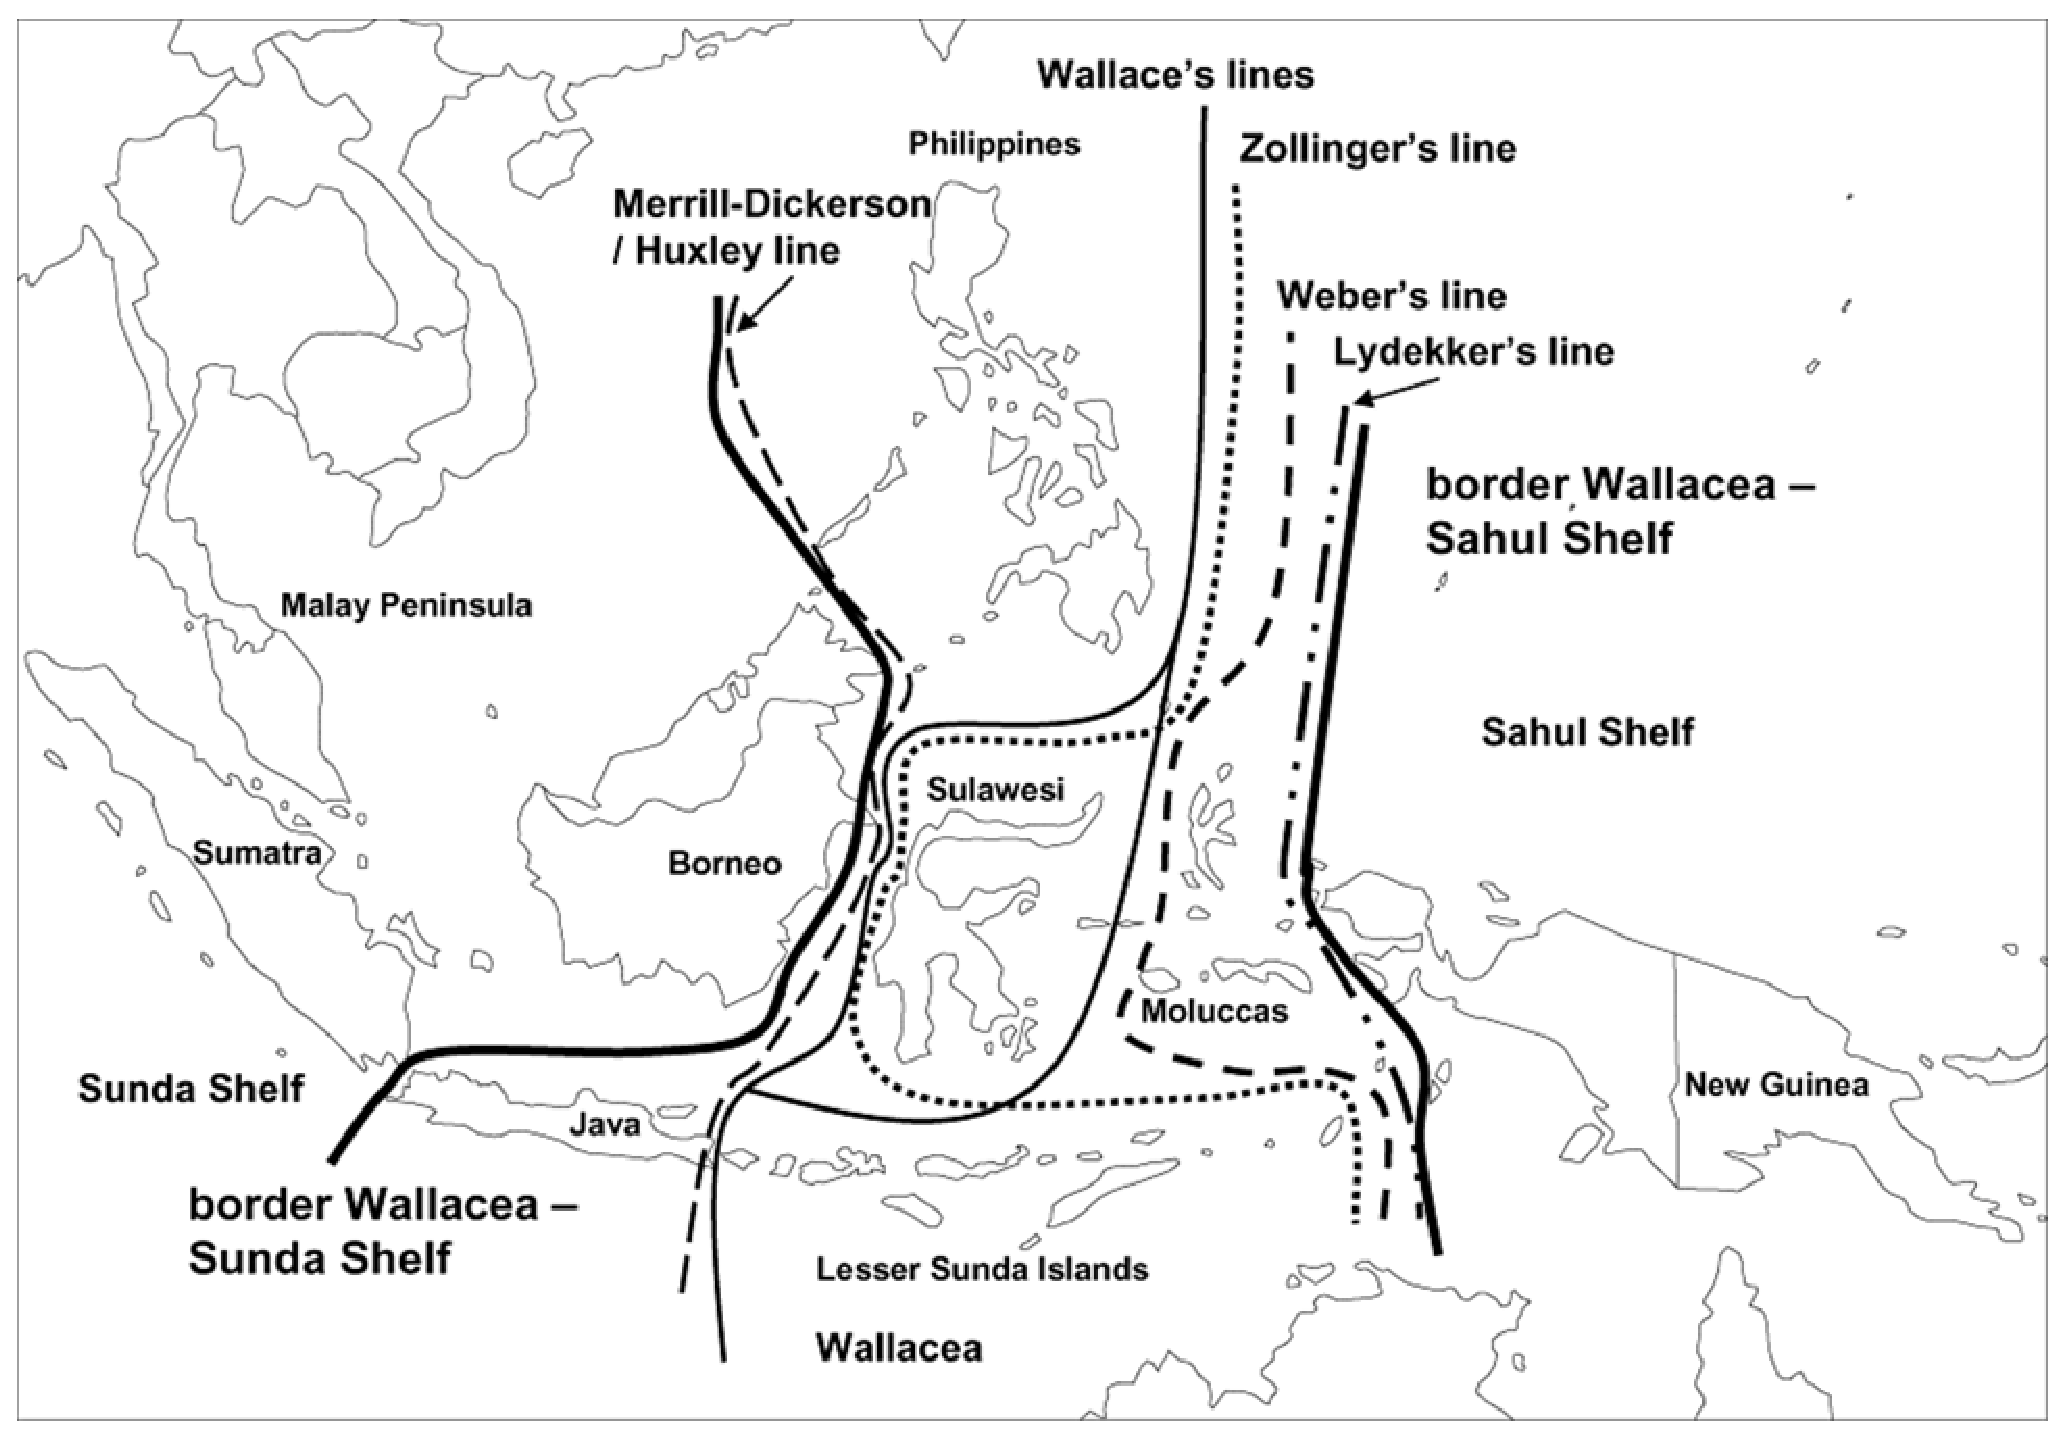
\includegraphics[width=1.0\textwidth]{figures/Wallacea2.eps}
\caption[Biogeographical demarcation lines in insular Southeast Asia]{Biogeographical demarcation lines in insular Southeast Asia. Wallace's Line is drawn here in two variants, one including Sulawesi, and another one excluding it. Biological Wallacea is traditionally delimited by Wallace's Line in the west, and Lydekker's Line in the east. Reprinted from \citealt{Welzen2011}, Biol J Linn Soc, © 2011 The Linnean Society of London.}\label{map:wallacea}

\end{figure}

Throughout this book, I will consider the western variant of Wallace's line loosely as the western boundary of the Eastern Indonesian area, and mainland New Guinea as the eastern boundary (extending biogeographical Wallacea beyond Lydekker's Line to comprise the Bird's Head area). Moving roughly from west to east, the whole area then consists of Sulawesi, the Lesser Sunda Islands (or Nusa Tenggara) including Timor, the Moluccas, and the western tip of Indonesian Papua. Turning now to linguistic data, we find that the area of Eastern Indonesia as sketched above is supported by both typological and historical-comparative evidence. I will in \sectref{sec:geneticlineage} start with an outline of the diachronic relations, presenting the languages of the EI sample in the context of their genealogical affiliation as suggested by historical-comparative evidence. In \sectref{sec:typo}, I will then shift the perspective to a typological overview, summarising recent research on Eastern Indonesia as a linguistic Sprachbund. 

\section{Genealogical lineage}\label{sec:geneticlineage}

The languages of Eastern Indonesia share a set of common ancestors, that is, they are in a genealogical relationship. This cannot always be traced by way of the traditional historical-comparative method. It is specifically within the Papuan languages that time depth is a challenging issue: the time frame starting from the point where proto-languages such as Proto-Trans--New Guinea split up and developed into separate directions up to the contemporary situation in linguistic Papua is tremendous. Given that the advent of Papuan-speaking communities in the New Guinea area dates back about 40,000 years BP, it does not come as a surprise that Papuan linguistics up to today can neither reconstruct a single Proto-Papuan ancestor nor link all branches together. The term \textit{Papuan} is thus to be understood as a cover term for a group of unrelated language families in a particular geographical area rather than as a genealogical concept. Recent work on the classification of Papuan languages made use of pronoun paradigms as diagnostic evidence for genealogical relations \citep{Ross2005}. Ross identified twenty-three families of Papuan languages all across New Guinea and its vicinity, among them the large Trans--New Guinea (TNG) family.

\subsection{Austronesian languages}

The Austronesian languages constitute a clear monophyletic group, and much work has been done to reconstruct the Proto-Austronesian lexicon, phonology, and grammar (recent contributions include, among others, \citealt{Tryon1995}, \citealt{wouk2002history}, \citealt{blust2009austronesian}; see \citealt{adelaar2005austronesian} for an overview). The whole Austronesian language family consists of some 1,200 languages and is considered the largest language family in the world with respect to the number of languages, and the second largest in terms of geographical distribution \citep{adelaar2005austronesian}. Having originated from Taiwan, Austronesian-speaking communities made their way as far west as Madagascar, as far east as Easter Island, and settled much of insular Southeast Asia, Melanesia, Micronesia, and Polynesia from Haiwai'i in the north to New Zealand in the south. All these groups can be traced back to the primary branch Malayo-Polynesian (MP). The other nine primary branch\-es never ventured out of Taiwan \citep{blust2009austronesian}. MP divides further into Western Malayo-Polynesian (WMP) and Central-Eastern Malayo-Polynesian (CEMP), both comprising some 600 languages. \citet{blust2009austronesian} names as the chief defining feature of WMP the presence of nasal substitution in active verb forms, often leading to segmental changes in the prefix and/or the root (cp. Malay \textit{pukul} `hit' (base form): \textit{me-mukul} (active form); \citealt[30]{blust2009austronesian}). Apart from this characteristic, it is still not clear whether WMP really constitutes a monophyletic group or rather a paraphyletic collection of residual branches that are not CEMP (cf. \citealt[30]{blust2009austronesian}). 

\begin{sidewaysfigure}
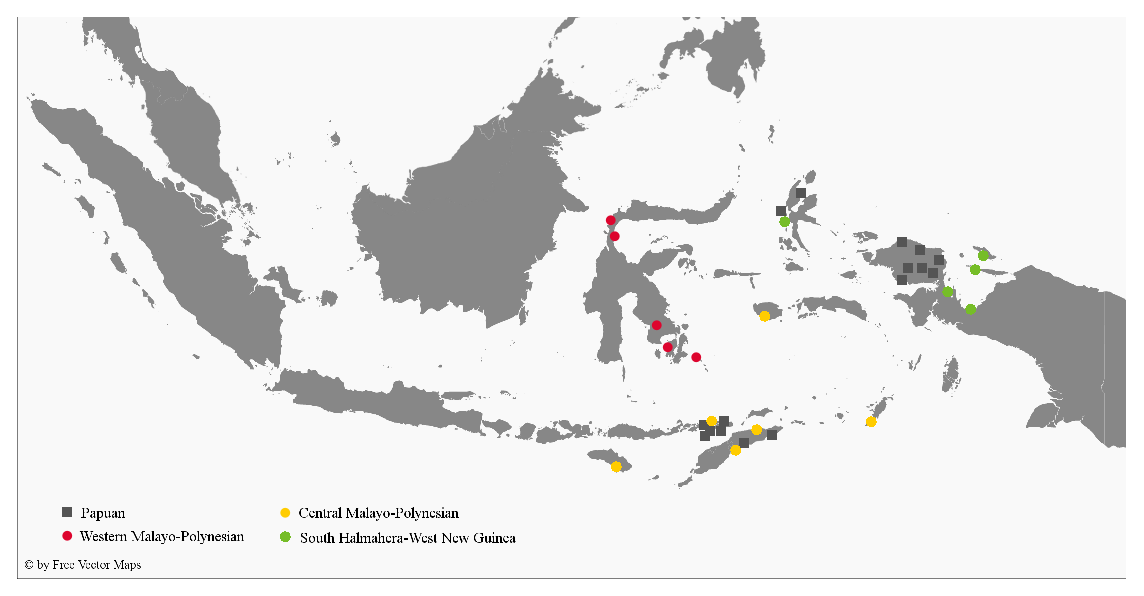
\includegraphics[width=\columnwidth]{figures/Map_overview_klein_Austroaff.eps}
\caption[Geographical distribution of Austronesian languages in the sample]{Geographical distribution of Austronesian languages in the EI sample. Colours indicate genetic affiliation to the different subgroups.}\label{map:Austro1}
\end{sidewaysfigure}

Central-Eastern Malayo-Polynesian, on the other hand, is firmly supported by phonological, lexical, morphosyntactic, and semantic innovations (see \citealt{blust1993central}) and seems now widely accepted. The 600 odd languages divide into a Central-Malayo-Poly\-ne\-sian branch (CMP) with about 120 languages, and an Eastern-Malayo-Polynesian (EMP) branch. The CMP languages are located in the Nusa Tenggara area, comprising the Lesser Sunda Islands from East Sumbawa eastwards, up to the Timor area and beyond into the southern Moluccas, including the Austronesian languages on the western extremities of Bomberai peninsula (Northern Bomberai languages \ili{Sekar}, \ili{Onin} and \ili{Uruangnirin}; \citealt[24]{adelaar2005austronesian}), but not the Halmahera archipelago north of Buru and Seram. Here, as well as in the Bird's Head area and around Cenderawasih Bay, we find 30--40 EMP languages of the South Halmahera-West New Guinea subfamily (SHWNG), which is the sister taxon of the Oceanic languages that have spread eastwards into Melanesia and greater Oceania \citep{blust2009austronesian}. The dividing line between the SHWNG languages in the west and the Oceanic languages in the east runs somewhere through the eastern end of Cenderawasih Bay, leaving \ili{Waropen} in the SHWNG group while the \ili{Sarmi languages} belong to the Oceanic subfamily. Thus all Austronesian languages in Eastern Indonesia (as defined in this book) either belong to WMP, CMP or to SHWNG. \figref{fig:Austro2} presents the internal genealogical division of the Malayo-Polynesian languages down to CMP and SHWNG, including the 16 Austronesian languages investigated in this book.

\begin{figure}

\begin{footnotesize}
\jtree[xunit=8em,yunit=2em]
\! = {Malayo-Polynesian}
:({WMP} {\psframebox{\begin{tabular}{c} \ili{Muna} \\ \ili{Pendau} \\ \ili{Tajio} \\ \ili{Tolaki} \\ \ili{Tukang Besi}  \end{tabular}}}) {CEMP}
:({CMP} {\psframebox{\begin{tabular}{c} \ili{Alorese} \\ \ili{Buru} \\ \ili{Kambera} \\ \ili{Selaru} \\ \ili{Tetun Fehan} \\ \ili{Waima'a}  \end{tabular}}}) {EMP}
:({SHWNG} {\psframebox{\begin{tabular}{c} \ili{Biak} \\ \ili{Dusner} \\ \ili{Mor} \\ \ili{Taba} \\ \ili{Wooi}  \end{tabular}}}) {Oceanic}.
\endjtree
\end{footnotesize}

\caption[The Malayo-Polynesian branch of Austronesian]{Tree diagram of the Malayo-Polynesian branch of the Austronesian language family. Genealogical affiliation after \citet{adelaar2005austronesian}. Boxed languages belong to the sample of EI languages investigated in this book.}\label{fig:Austro2}
\end{figure}


\subsection{Papuan languages}

Quite unlike the Austronesian family, there is up to now no convincing hypothesis that would link the Papuan languages in Eastern Indonesia to a single common ancestor \citep{reesink2005west, klamer2008east}. Papuan languages in EI come in three major areal groupings: (i) the Papuan languages spoken on the islands of Alor and Pantar off the Timorese north coast, as well as the languages located on Timor and the small island of Kisar (\textsc{TAP} languages); (ii) the Papuan languages of North Halmahera (NH); and (iii) the Papuan languages of the Bird's Head area, including the isolate \ili{Yawa} on Yapen island in Cenderawasih Bay. Several hypotheses on their genealogical relationship (as well as their connection to the Papuan languages further to the east) have been discussed. The TAP languages have been placed among the Trans--New Guinea phylum and links have been postulated between TAP and the West Bomberai languages, most recently by \citet{Ross2005}, who proposed that they are part of the TNG ``Western Linkage", based on a pronominal innovation in the first person plural \citep[9]{schapper2014intro}. The NH languages, on the other hand, have been placed with the West Papuan languages from the Bird's Head area, most prominently with those of the West Bird's Head family (see \citealt{reesink2005west} for an overview).

\begin{sidewaysfigure}
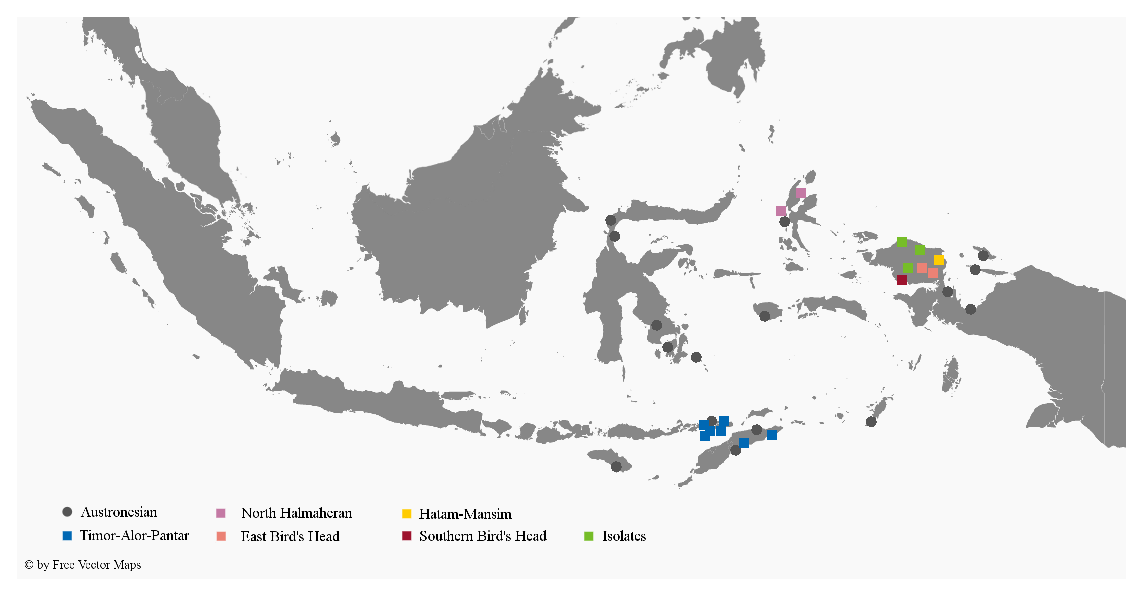
\includegraphics[width=\columnwidth]{figures/Map_overview_klein_Papuaff.eps}
\caption[Geographical distribution of Non-Austronesian languages in the sample]{Geographical distribution of Non-Austronesian languages in the EI sample. Colours indicate genealogical affiliation to the different taxa. Language isolates are given in green.}\label{map:Austro2}
\end{sidewaysfigure}

The TAP languages comprise some 30 languages and divide into two main branches, the Alor-Pantar languages (\textsc{AP}) and the Timor-Kisar languages (\textsc{TK}). Both subgroups, as well as the TAP branch in general, have recently been established by comparative work \citep{holton2012historical, klamer2014alor}, although a genealogical link between the languages was hypothesised before \citep[7]{schapper2014intro}. While the relationship between the five Timor-Kisar languages seems quite well understood, the internal subgrouping of the AP languages is still under discussion. \figref{fig:timor-alor-pantar} shows a tree diagram of the TAP branch. Seven TAP languages, two TK languages and five AP languages, have been included in the sample.

\begin{figure}

\begin{footnotesize}
\jtree[xunit=5em,yunit=2em]
\! = {Timor-Alor-Pantar}
:[scaleby=2 1]{Alor-Pantar}!a {Timor}
:{\psframebox{\ili{Bunaq}}} {East Timor}
:{Makasae-Makalero}!b {Fataluku-Oirata}
<left>[scaleby= .5 1]{\ili{Fataluku}} ^<right>[scaleby= .5 1]{\ili{Oirata}}.
\!a = <tri>{AP languages}{\psframebox{\begin{tabular}{c} \ili{Abui} \\ \ili{Kaera} \\ \ili{Klon} \\ \ili{Teiwa} \\ \ili{Western Pantar} \end{tabular}}}.
\!b = <left>[scaleby= .5 1]{\ili{Makasae}} ^<right>[scaleby= .5 1]{\psframebox{\ili{Makalero}}}.
\endjtree
\end{footnotesize}

\caption[The Timor-Alor-Pantar languages]{Tree diagram of the Timor-Alor-Pantar languages, as proposed by \citet{schapper2014intro}. Boxed languages belong to the sample of EI languages used in this book.}\label{fig:timor-alor-pantar}
\end{figure}

The North Halmaheran language family is supported by lexicostatistic evidence and appears now generally accepted (e.g. \citealt{Voorhoeve1994, reesink2005west}). The languages are located on the northern part of Halmahera, including Morotai and the small volcano islands just off the western shore. NH consists of three related language groups, \ili{Northeast Halmaheran}, \ili{Sahu}, and \ili{Ternate}-\ili{Tidore}, as well as the family level isolate \ili{West Makian} \citep{Voorhoeve1994}. While Voor\-hoeve listed the Northeast Halmaheran group as a chain of closely related dialects, contemporary research supports the view that the different varieties are in fact distinct languages rather than dialects. One of the main arguments is that mutual intelligibility is hard to put to the test in areas with extensive multilingualism (see \citealt{holton2003tobelo} on Tobelo; a similar argument is made by Schapper on the TAP languages, see \citealt[3]{schapper2014intro}). Therefore, the rate of real intelligibility would actually be lower if there were no cultural practice of multilingualism. \figref{fig:halmahera} depicts the internal relationship of the NH languages, including the varieties of Northeast Halmaheran. Two languages from this language family, Tobelo and Tidore, have been included in the EI sample.

\begin{figure}
\begin{footnotesize}
\jtree[xunit=8em,yunit=2em]
\! = {North Halmaheran}
:{North Halmaheran}!a ({Family level isolate}{West Makian}).
\!a = <left>{Northeast Halmaheran}{\begin{tabular}{c} \ili{Galela} \\ \ili{Loloda} \\ \ili{Modole} \\ \ili{Pagu} \\ \ili{Tabaru} \\ \psframebox{\ili{Tobelo}}  \end{tabular}} ^<vert>{\ili{Sahu}} ^<right>{Ternate-Tidore}{\begin{tabular}{c} \psframebox{\ili{Tidore}}  \end{tabular}}.
\endjtree
\end{footnotesize}

\caption[The North Halmaheran language family]{Tree diagram of the North Halmaheran language family, following \citet{Voorhoeve1994} and \citet{holton2003tobelo}. Boxed languages belong to the sample of EI languages used in this book.}\label{fig:halmahera}
\end{figure}

The third Papuan grouping (Bird's Head languages of Western Papua) shows a more complicated internal pattern, and the different groups have hitherto resisted the reconstruction of a common ancestor. A fairly traditional approach to the genealogical relationship in the area was the postulation of two main taxa: first, the West Papuan languages, including the Bird's Head languages without the South Bird's Head (SBH) family, and second, the Trans New Guinea phylum, represented in Western Papua by the SBH languages and the West Bomberai subgroup. This dichotomy, however, has recently been called into question as research on the Bird's Head languages has advanced \citep{dol2007grammar}, and more cautious approaches now distinguish a range of smaller sized families \citep{reesink2005west}.

The relationship within some of these subgroups is well established by now. There is evidence that the Papuan languages along the Head's western shore form a coherent group, comprising \ili{Moi}, \ili{Tehit}, \ili{Moraid} and \ili{Seget} (The West Bird's Head family (WBH)). Along the northern shore and further inland, we find a set of unrelated isolates, namely \ili{Abun}, \ili{Mpur}, and \ili{Maybrat}. Finally, there is the East Bird's Head family, consisting of \ili{Meyah}, \ili{Moskona} and \ili{Sougb}, and the \ili{Hatam}-\ili{Mansim} group on the north-eastern part of the Bird's Head. Following \citet{klamer2008east}, we can establish the list of genealogically related subgroups as shown in \figref{fig:westpapuan} of which seven languages are part of the EI sample.


\begin{figure}[ht]
{\raggedright%
\begin{footnotesize}
\textit{Cenderawasih Bay} \\
(1) \ili{Yawa} (isolate) \bigskip\\
\textit{Northern Bird’s Head, with three families and three isolates} \\
(2) East Bird’s Head family: \ili{Meyah}; \psframebox{\ili{Moskona}}; \psframebox{\ili{Sougb}} \\
(3) West Bird’s Head family: \ili{Moi}; \ili{Tehit}; \ili{Moraid}; \ili{Seget} \\
(4) \psframebox{\ili{Hatam}} and (extinct) \ili{Mansim} \\
(5) \psframebox{\ili{Mpur}} \\
(6) \psframebox{\ili{Maybrat}} \\
(7) \psframebox{\ili{Abun}} \bigskip\\
\textit{Southern Bird’s Head} \\
(9) The Trans New Guinea family with two subgroups: \\
– South Bird’s Head, with \psframebox{\ili{Inanwatan}} \\
– West Bomberai: \ili{Iha}, \ili{Baham} \\
\end{footnotesize}}
\caption[The Papuan languages of the Bird's Head]{Papuan language families in the Bird's Head area, following \citet{klamer2008east}. Boxed languages belong to the sample of EI languages used in this book.}\label{fig:westpapuan}
\end{figure}

Summing up the genealogical situation in EI, we find both Austronesian and non-Austronesian language communities. While the Austronesian languages are fairly well connected by a shared linguistic history, it has proven difficult to formulate an uncontroversial genealogical reconstruction for the non-Austronesian languages. The TAP languages provide a link to the vast TNG language family in mainland Papua. The North Halmaheran languages as well as the bulk of Papuan languages in the Bird's Head, on the other hand, do not seem to be related to TNG. 

The boxed languages from all taxa presented in Figures \ref{fig:Austro2}--\ref{fig:westpapuan} make up a total of 32 languages, including 16 Austronesian languages and 16 Papuan languages, and together constitute the data source of this study. In the next section, I will put the languages into the context of a shared areal history of mutual contact, resulting in the convergence of features, both Wallacean and Melanesian.

\section{Typological features}\label{sec:typo}
In most situations where different linguistic communities live in close proximity to one another, there is language contact through trade, inter-marriage, warfare, and other kinds of interaction. Scenarios of contact constitute one of the major forces that cause languages to change over time \citep{thomason2001language}. Such contacts not only lead to language change but over longer periods to language convergence and the formation of linguistic areas, in which common structural features diffuse into the different languages. The area that biogeographically forms Wallacea is known for extended periods of language contact between different social groups. \citet[141f.]{schapper2015wallacea} lists archaeological evidence for pre-Austronesian contacts in Wallacea: pelagic fish hook finds from East Timor suggest the existence of a pre-Austronesian seafaring people in the area more than 5,000 years before Austronesian arrival. Rock art motifs from Timor and Bomberai peninsula show similar traits, which suggest prehistoric contact between different communities beginning before 20,000 BP. Obsidian finds from Timor dating back up to 13,000 BP point to ancient inter-island trading routes. Finally, the anthropogenic introduction of Australasian marsupial species into the Wallacea area (for instance the Northern common cuscus \textit{Phalanger orientalis}) confirms human impact across zoogeographical subregions (see also \citealt{Heinsohn2010}).

Moving down to historical times, evidence from trade of natural resources indigenous to the Moluccas, such as clove, nutmeg and mace, suggests that there were ancient trade routes in place as early as 2,000 years BP \citep{klamer2008east}. The 15th century saw the advent of Islam in Ternate and Banda, and in the subsequent centuries, the ``Malayo-Muslim trading network" expanded throughout western Indonesia and well into the eastern parts \citep{klamer2008east}. One of the most important driving forces for inter-cultural contact in the eastern area was certainly the slave trade and raid routes that were established at the very latest with the rise of the kingdoms of Ternate and Tidore from the 13th century onward \citep{klamer2008east}. These routes extended well into the Bird's Head area, where the power and influence of the Sultans was exerted by dominant cultural groups such as the Biak people in the Cenderawasih Bay area \citep[2]{vanheuvel2006} or the Onin ``middle men" along the Bird's Head south coast that had the title \textit{raja} `king' \citep[2]{devries2004}. De Vries reports that these trading networks into the Bird's Head area stimulated situations of extensive language contact:

\begin{quote}There were \textit{raja}'s in the villages Rumbati, Patipi, Ati-Ati and Fatagar and each \textit{raja} had its own section of the Bird's Head south coast where he had some influence through representatives who settled near river mouths. The \textit{raja} of Patipi sent representatives to the Siganoi river mouth where they engaged in slave trade with the Inanwatan people. To get slaves, the Inanwatan raided the interior but also neighbouring coastal peoples like the Yahadian. In exchange for the slaves, they received cloths, iron tools and weapons and guns from the Patipi ``middle men". Although these \textit{raja}'s of Patipi never established a regular government in the Inanwatan area, the Patipi colonists in Inanwatan married local women and Patipi words were borrowed by the Inanwatan language.\end{quote}

The dominant position of these regional agents of the Sultanates had important linguistic consequences all across the region, as their native languages gained the prestige typical for ruling groups. \ili{Biak} and \ili{Onin} thus became local lingua francas in their respective areas of dominance, as did \ili{Ternate} and \ili{Tidore} across the wider Moluccan area, and \ili{Malay} varieties throughout all of Eastern Indonesia. When the first Europeans arrived in the area, they not only found the regional kingdoms to dominate an entire trading economy but also a slave trade along the New Guinean coasts, into the Moluccas, and the islands further south that had caused much interethnic mixing. Consequently, many slaves from mainland Papua lived among the populations on Tidore and Ternate. This situation must have led to ``the displacement of Austronesian speakers to non-Austronesian speaking areas, and vice versa" \citep[105f.]{klamer2008east}.

All these historical facts suggest that Wallacea was indeed a place of prolonged and intensive language contact, and, not unexpectedly, this is reflected in shared linguistic features throughout the area. Several authors have discussed sets of common features, and some of them recently suggested a Sprachbund scenario for the area. In the following sections, I will briefly introduce three approaches that highlight the shared linguistic background: Himmelmann's typological profile of Austronesian preposed possessor languages (\sectref{sec:preposed}), Klamer, Reesink and van Staden's approach to East Nusantara as a linguistic area (\sectref{sec:nusantara}), and Schapper's proposal of linguistic Wallacea as a Sprachbund (\sectref{sec:wallacea}). Further Papuan-related features that are found across the Papuan language families in the Bird's Head area and beyond are discussed in \citet{reesink2005west} (briefly reviewed in \sectref{sec:westpapuan}).

\subsection{Preposed possessor languages}\label{sec:preposed}

Working on the Austronesian languages of insular Southeast Asia, \citeauthor{Himmelmann2005austronesian} proposed a typological subdivision of the western Austronesian languages\footnote{The 
    term \textit{Western Austronesian} is a purely geographical expression and should not be confused with the phylogenetic branch of Western Malayo-Polynesian. See \citet{Himmelmann2005austronesian} 
    for further explanation.
}
(excluding the Oceanic branch) into \emph{symmetrical voice languages} and \emph{preposed possessor languages} \citep{Himmelmann2005austronesian}. He argues that symmetrical voice and preposed possessors are mutually exclusive in most languages, and that each of these features clusters with further typological features \citep[113]{Himmelmann2005austronesian}. Symmetrical voice languages are defined by the presence of two or more voice patterns (similar but not equivalent to active vs. passive) none of which can be considered the basic form. The most prototypical representatives of symmetrical voice languages are found within the group of the so-called Philippine-type languages (for instance the well-researched \ili{Tagalog} voice system; \citealt{schachter1976subject}, \citealt{Himmelmann2005tagalog}, \citealt{riesberg2014symmetrical}), which Himmelmann defines as having the following additional characteristics:

\begin{itemize}
\item at least two formally and semantically different \textit{undergoer} voices
\item at least one non-local phrase marking clitic for nominal expressions (e.g. \ili{Tagalog} genitive \textit{ng})
\item pronominal second position clitics
\end{itemize}

These features exclude other symmetrical voice languages like \ili{Malagasy}, \ili{Chamorro} as well as the Tomini-Tolitoli\il{Tomini-Tolitoli languages}, Gorontalo-Mongondic\il{Gorontalo-Mongondic}, Sama-Bajau\il{Sama-Bajau languages}, and \ili{South Mindanao languages} that are spoken in Northern Sulawesi, the southern Philippines, and environs \citep[113]{Himmelmann2005austronesian}. The five languages from Sulawesi are the only symmetrical voice languages included in the sample.

Preposed possessor languages, on the other hand, are primarily defined as placing the possessor before the possessum in possessive constructions. This type of language is predominantly found in the eastern parts of Indonesia and appears most often to have either asymmetrical voice alternations or no voice alternations at all. For instance, in the Austronesian language \ili{Waima'a}, spoken in East Timor, the most common possessive construction shows a preposed possessor order, as in \textit{hire buu} (1\textsc{pl}.\textsc{in} ancestor) `our ancestors' or \textit{mata umo-n} (dead house-\textsc{poss}) `the deceased's house' \citep[31]{bowden2006} .\footnote{There is also a less common postposed possessor construction in \ili{Waima'a} where the possessor is overtly marked by final \textit{nini}. This construction, however, is functionally more specific as it appears to focus the possessor, and permits the omission of the possessed entity (see \citealt[32]{bowden2006})} The dividing line between symmetrical voice languages and preposed possessor languages roughly cuts through the western Lesser Sunda Islands and runs east of Sulawesi, dividing linguistic Eastern Indonesia in two parts: a smaller western portion, consisting of Sulawesi and the westernmost Lesser Sunda Islands Bali, Lombok, Sumbawa and possibly Flores, and a greater eastern part comprising eastern Nusa Tenggara, Timor, the Moluccas and the western tip of mainland Papua. \figref{figure:preposed} shows the distribution of possessive constituent orders in selected languages throughout Indonesia, illustrating the clustering of preposed-possessor languages (blue) in the east and postposed-possessor languages (red) in the west. The map is adapted from WALS (World Atlas of Language Structures; \citealt{wals-86}) and thus does not display all languages that are part of the EI sample.

\begin{sidewaysfigure}
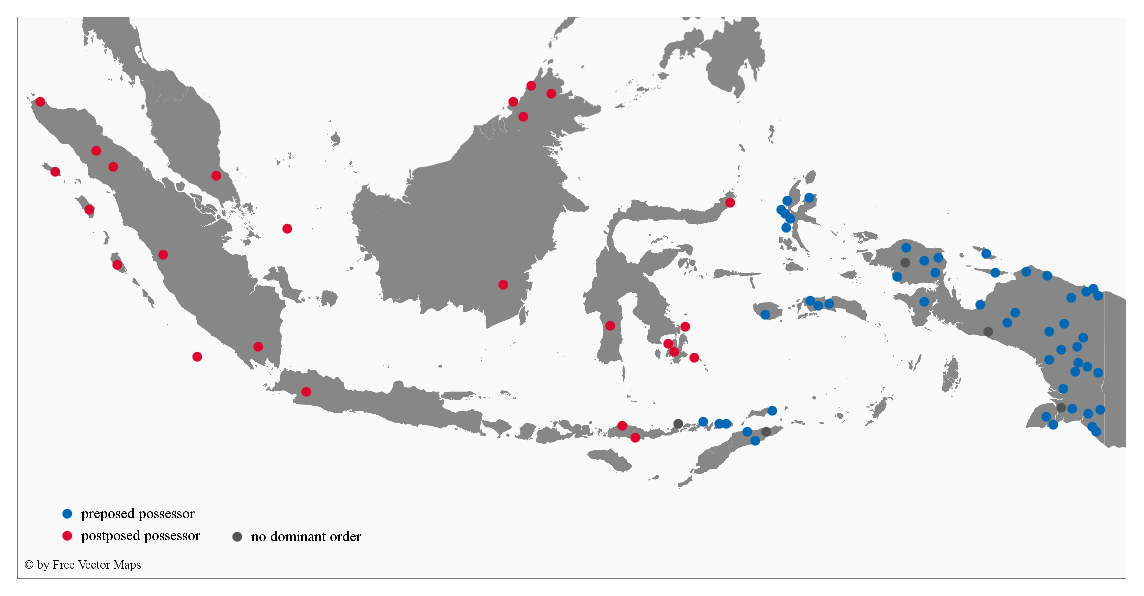
\includegraphics[width=\columnwidth]{figures/Preposed_possessor.eps}
\caption[Order of possessor and possessum in Western Austronesian languages]{Order of possessor and possessum in Western Austronesian languages. Blue circles designate preposed possessor languages, red circle languages show the opposite order with the possessum before the possessor. Grey languages do not have a clear preference. Adapted from \citet{wals-86}.}\label{figure:preposed}
\end{sidewaysfigure}

What makes the distinction into symmetrical voice languages and preposed possessor languages typologically useful is that these parameters are reported to match with values of further parameters. \tabref{table:sympre} gives an overview of the feature complex for both typological subgroups. 

\begin{table}[ht]
\begin{tabularx}{\textwidth}{QQ}
\lsptoprule
Symmetrical voice languages & Preposed possessor languages \tabularnewline
\midrule
Symmetrical voice alternations & No or asymmetrical voice alternations \tabularnewline
Postposed possessor & Preposed possessor \tabularnewline
No alienable/inalienable distinction & Alienable/inalienable distinction \tabularnewline
Few or no differences between narrative and equational clauses & Clear-cut differences between narrative and equational clauses \tabularnewline
Person marking only sporadically attested & Person marking prefixes or proclitics for S/A arguments \tabularnewline
Numerals/quantifiers precede head & Numerals/quantifiers follow head \tabularnewline
Negators in pre-predicate position & Clause-final negators \tabularnewline
V-initial or SVX & V-second or -final \tabularnewline
\lspbottomrule
\end{tabularx}
\caption[Characteristic features of symmetrical voice and preposed possessor languages]{Characteristic features of symmetrical voice and preposed possessor languages according to \citet[175]{Himmelmann2005austronesian}.}
\label{table:sympre}
\end{table}

It is certainly not the case that all Austronesian languages in Eastern Indonesia invariably show all preposed possessor features (person marking, for instance, is absent in a group of isolating Austronesian languages spoken on Timor, see \citealt[175]{Himmelmann2005austronesian}) but chances are high that they have at least some of them. 

\subsection{East Nusantara as a linguistic area}\label{sec:nusantara}

The last section presented evidence that the Austronesian languages in Eastern Indonesia converge on a number of typological features. Turning now to the Papuan languages in the area, we observe that most of these features are shared by them as well, and there have been claims that some of the features listed by Himmelmann are in fact of Papuan origin. \citet{klamer2008east} argue for a linguistic area in Eastern Indonesia which they call East Nusantara (Nusantara is a Malay term meaning `the islands in-between', from \textit{nusa} `island' and \textit{antara} `between'; see \citealt[99]{klamer2008east}). According to their definition, East Nusantara includes all islands along the Sunda-Banda chains, from Flores in the west and Halmahera in the north, up to the Bird's Head region of Indonesian Papua, and is thus roughly consistent with my depiction of Eastern Indonesia, with one major exception: Sulawesi is excluded from East Nusantara, although the authors note that 

\begin{quote}[t]here is clear evidence that the inhabitants of East Nusantara travelled to places outside the area, and there are genealogical relations between languages of this area and languages outside it. Especially parts of Sulawesi and New Guinea, not included at present, may have to be incorporated later.\end{quote}

In their analysis of East Nusantara linguistic features, the authors argue that the following Papuan features diffused into both Austronesian and non-Aus\-tro\-ne\-sian languages (in Eastern Indonesia): alienability, order of possessor and possessum in adnominal possession, and clause-final negators. Evidence that tone also spread from Papuan to Austronesian languages is considered weak.

The distinction between alienable and inalienable possession is a lexically conditioned effect that divides up the noun system of a language into two or more subsets (for instance, in distinguishing between entities with external relation to the possessor vis-à-vis internal relations such as kin, part-whole relations etc). It is absent from most western Austronesian languages but occurs in Central-Eastern Malayo Polynesian (CEMP) languages that are spoken in close vicinity to Papuan speaking communitites in EI \citep[116]{klamer2008east}. The Papuan languages in the area have this distinction. Thus, while historical-comparative approaches have attempted to present the alienability distinction as a shared innovation inside the CEMP subgroup \citep{blust1993central}, typologists more recently argued for a Papuan feature that had made its way into the Austronesian languages of EI.  

Possessive classification can be found as far west as Sulawesi. \ili{Tukang Besi}, for instance, shows different ways of construing (phrasal) possession, and these construals are sensitive to lexical classes. Consider the following example from Tukang Besi where the possessive determiner \textit{nu} connects the possessed item to a possessor.

\ea 
\langinfo{Tukang Besi}{Austronesian, WMP}{\citealt[339]{donohue1999}}\\
\gll te kadera nu ama-su\\
\textsc{core} chair \textsc{gen} father-\textsc{1}\textsc{sg}.\textsc{poss}\\
\glt ‘my father's chair’
\z

In Tukang Besi, there are two features of adnominal possession that give rise to an alienable/inalienable interpretation. First, \textit{nu} is preferentially left out when it comes to ``possession of a kin term, or the `possessive relation' expressed between a person and their village, island or ethnic group" \citep[346]{donohue1999}. Second, there is a distinct possessive construction that appears to mark inalienable possession overtly by use of the element \textit{mai}. \textit{Mai} has at least two different meanings, depending on the status of the possessed noun. With close kin nouns, the reading is that the item is inalienable from its possessor. The same reading may be invoked with ordinary objects like houses or canoes. The only difference is that in those cases a sense of plurality is associated with the objects. The core system, however, seems to be sensitive to close family kin terms, so that we may say that the set of nouns in Tukang Besi is subdivided into two types (although the \textit{mai} construction is, outside its core semantics with kinship terms, basically a pragmatic device). 

If possessive classification constitutes an areal feature marking language contact and the presence of a linguistic area, this area exerts influence beyond the borders of East Nusantara \textit{sensu} \citet{klamer2008east} and into parts of neighbouring Sulawesi. In her discussion of linguistic Wallacea, Schapper notes that ``[t]he Melanesian feature with the widest reach beyond New Guinea is possessive classification" \citep[108]{schapper2015wallacea}, extending far into Melanesia and the Oceanic languages. This eastern spread appears to be weakly mirrored by the western spread of possessive classification systems in Sulawesi languages, beyond East Nusantara proper. Almost all Papuan languages of Eastern Indonesia show the alienability/inalienability distinction. This has led \citet[120]{klamer2008east} to the conclusion that

\begin{quote}[a]lthough it is not a universal feature in the Papuan languages,
the distinction between alienable and inalienable possession is found in a number of different Papuan families [...] and can be seen as a `Papuan trait’.\end{quote}

With regard to the Austronesian languages in the area, they report that the languages east of Timor typically make the alienability/inalienability distinction, while the Timor languages as well as the languages to the west show a more varied pattern. Interestingly, they claim that, among others, \ili{Tukang Besi} does not mark alienability \citep[120]{klamer2008east}, while Schapper apparently does include \ili{Tukang Besi} in the group of languages that show possessive classification (judging from the map in \citealt[110]{schapper2009bunaq}). As we have seen above, the interplay between \textit{nu} and \textit{mai} encodes the concept of alienable/inalienable possession at least in some contexts, so that Schapper's classification appears justified.

The second feature claimed to be of Papuan origin is the order of possessor and possessum. Klamer and colleagues show that both Papuan languages with SOV constituent order as well as many Papuan SVO languages have preposed-possessor order, at least with inalienable possession and a full NP possessor \citep[123f.]{klamer2008east}. There are, however, hybrid patterns. In \ili{Maybrat}, spoken in central Bird's Head, the order shifts to possessum-possessor in alienable possession. Consider the following pair of examples. In (\ref{Maybrat_Klamer_b}), the relating element \textit{ro} marks a possessum-possessor construction, while in (\ref{Maybrat_Klamer_a}), inalienable possession shows preposed possessor order without any linking element.

\ea
\langinfo{Maybrat}{Papuan, isolate}{\citealt[119]{klamer2008east}}\\
\ea \label{Maybrat_Klamer_a}
\gll fnia m-ao\\
woman \textsc{3}\textsc{u}-foot\\
\glt ‘the woman's foot’
\ex \label{Maybrat_Klamer_b}
\gll amah ro t-atia\\
house \textsc{poss} \textsc{1}\textsc{sg}-father\\
\glt ‘my father's house’
\z
\z

Another feature that seems to be Papuan in origin is clause-final negator placement (\textit{post predicate negation} in \citealt{klamer2008east}). Recall that this feature is used by \citet{Himmelmann2005austronesian} as a correlate for his preposed possessor languages. Yet, from a typological perspective, clause-final negation is more common with SOV word order, and is therefore rather unexpected for Austronesian languages with predominant VSO or SVO constituent orders \citep{klamer2008east}. It is, however, well known from several groups of Papuan languages, such as the Trans-New-Guinea languages, the South Bird's Head languages like \ili{Inanwatan}, as well as the Papuan languages of Timor, Alor and Pantar (for instance from \ili{Western Pantar}, \ili{Kaera} and \ili{Sawila}),  languages along the north coast (\ili{Sentani}), some of the Torricelli phylum languages, and East Papuan languages \citep{klamer2008east}. Clause-final negator placement seems also to be present in some of the Papuan languages of Halmahera (\ili{Tobelo} has a predicate-final suffix \textit{-ua}, \citealt{holton2003tobelo}; but see \citealt[131]{klamer2008east}).

In Austronesian languages outside East Nusantara, the typical negation pattern is pre-verbal/pre-predicate or clause-initial. In Eastern Indonesia, however, we do find a number of Austronesian languages with clause-final negation, especially in the eastern parts. \ili{Wooi} is an example, as well as \ili{Dusner}, \ili{Biak}, and \ili{Windesi Wamesa} \citep{gasser2014windesi}, all of which show a related formative \textit{va} (which might be a reflex of a borrowed negator from a West Papuan language that has diffused into the area, as \citet{reesink2002eastern} argues). Another example of clause-final negation is the marker \textit{te} in \ili{Taba}, spoken in the Moluccas. These cases notwithstanding, a sizeable amount of Austronesian languages from East Nusantara apparently withstood Papuan influence and still show pre-verbal/pre-predicate negation. Some languages of Timor seem to have retained this pattern (for instance \ili{Waima'a}, see also \citealt[132]{klamer2008east}), and the same goes for some languages further to the west, e.g. \ili{Kambera} (but not \ili{Alorese}), and the Sulawesi languages (for instance \ili{Muna} and \ili{Tukang Besi}). Eastern outliers of the pre-verbal/pre-predicate pattern can also be found in the Moluccas, where, for instance, \ili{Selaru} has a pre-verbal negator \textit{lema} \citep[140]{coward2005}. And \ili{Tetun Fehan} (Timor) shows a hybrid pattern involving two general negators \textit{la} and \textit{ha'i}: the former occurs in pre-predicate position, and the latter in post-predicate position \citep[228]{vanklinken1999grammar}.

According to \citet{klamer2008east}, the alienable/inalienable distinction, the preposed possessor order as well as clause-final negation are clearly Papuan traits that have percolated into neighbouring Austronesian languages in the East Nusantara linguistic area. Other features seem to have taken the opposite direction and originated in Austronesian languages. These are (i) SVO constituent order, and (ii) the inclusive/exlusive distinction. Both features have spread to some of the Papuan languages of the area. All Austronesian languages in the East Nusantara area show SVO word order \citep[113]{klamer2008east}. Among the non-Austronesian languages we find SOV order, a typical Papuan feature, in the Alor-Pantar languages as well as in the Papuan languages of Timor. North Halmahera and the Bird's Head region seem to be more heterogeneous and feature both SVO and SOV languages (SVO being more common in the Bird's Head; exceptions are the SBH languages, i.e., \ili{Inanwatan}, as well as language isolate \ili{Yawa} on Yapen island). Among the NH languages, \ili{Sahu}, \ili{Ternate}-\ili{Tidore} and \ili{West Makian} have been reported to have shifted from SOV to SVO, and the same appears to have happened in \ili{Pagu} \citep[114]{klamer2008east}. Closely related \ili{Tobelo}, on the other hand, still shows predominant SOV order, which, as \citet[55]{holton2003tobelo} reports, ``distinguishes Tobelo from most of its NH neighbors". He goes on in noting that VO constituent order is also available in Tobelo, as is the case in most of the Papuan SOV languages.

The inclusive/exclusive opposition in first person plural pronouns and subject indexers marks a contrast between `we, including you' and `we, excluding you'. Inclusive/exclusive is a widespread feature all across Austronesia, and almost all languages have this contrast \citep{Tryon1995,klamer2008east}. The Austronesian languages in East Nusantara agree with this pattern. Even languages with considerable exposure to Papuan neighbours and clear Papuan traits in their make-up still retain the inclusive/exclusive opposition, for instance Alorese \citep{klamer2011alorese}. Exceptions to the rule are only found in Malay varieties such as the ones spoken in the Northern Moluccas, the Alor-Pantar area \citep{klamer2008east}, as well as in varieties of Papuan Malay on mainland Papua \citep{kluge2014grammar}. With regard to the Papuan languages in the area, \citet[115]{klamer2008east} note that \begin{quote}in East Nusantara, it appears that the inclusive/exclusive distinction for the first person plural, a typically Austronesian feature,
occurs just in those Papuan languages that have had a long history of contact with surrounding Austronesian languages.\end{quote}
This includes the East Bird's Head family (EBH), Meyah and Sougb, as well as the West Bird's Head family (WBH), and the SBH family with Inanwatan, but not Maybrat, Abun and Mpur. In the other Papuan taxa of East Nusantara, it is even more widespread: almost all of the Timor-Alor-Pantar languages (TAP) and the Papuan languages of North Halmahera make the distinction with very few exceptions \citep[115]{klamer2008east}. 

\subsection{Linguistic Wallacea}\label{sec:wallacea}

Another approach to defining a linguistic area in Eastern Indonesia has recently been proposed by \citet{schapper2015wallacea}. Analogous to biological Wallacea, she argues for a linguistic Wallacea that comprises Nusa Tenggara including Timor, the Moluccas, the Bird’s Head, and Cenderawasih Bay, but not Sulawesi. Schapper's linguistic Wallacea is thus roughly commensurate with Klamer and colleagues' East Nusantara except that Schapper includes the lesser Sunda Islands up to Lombok (conforming to the Wallace line here), while \citet{klamer2008east} exclude the islands west of Flores. By taking into account the wider linguistic context east of Wallacea, Schapper argues that some of the EI areal features actually belong to a much larger zone of Melanesian influence. These include negator placement (clause-final negation), noun-numeral (postposed numeral) and genitive-noun (preposed possessor) orders, presence of possessive classification, complex numerals below ten as well as absence of the velar nasal /ƞ/. The first three features have been mentioned above. Possessive classification includes all types of possessive noun classes and is thus a broader phenomenon than the alienable/inalienable distinction which it includes. Possessive classification is further defined by distinct possessive constructions for each class. It is common in most Austronesian and Papuan languages of Eastern Indonesia and mainland Papua (although many central highland languages and a number of north coast Papuan languages do not have it) and spreads far into Oceania \citep[109]{schapper2015wallacea}.

The next feature, complex numerals below ten, refers to the compositional nature of numerals between six and ten in many languages that are located close to or on mainland Papua. Complex numerals may either be derived by adding up component numbers (e.g. in Mambae (Austronesian, Timor), the term `eight' is \textit{lim nai telu} [5+3]), by subtracting them (e.g. `eight' in Pak (Austronesian, Admiralty Islands) is \textit{arhuo} [10-2]), or by multiplication (e.g. \textit{ɹua mbhutu} [2x4] means `eight' in Rongga (Austronesian, Flores); \citealt[113]{schapper2015wallacea}). The distribution pattern of complex numerals stretches from Flores and Sulawesi in the west throughout Eastern Indonesia, continues along the Papuan north coast up into the Bismarck Archipelago, and reaches Vanuatu and New Caledonia in the east \citep[112--4]{schapper2015wallacea}. For Sulawesi, Schapper reports that some South Sulawesi languages show subtractive complex numerals `eight' and `nine', while \ili{Makasarese} has additive `seven' \citep[113f.]{schapper2015wallacea}. The Sulawesi complex numerals are listed as outliers, but may as well be taken to confirm a connection between the core area of Eastern Indonesia and Sulawesi.

The last feature of the Melanesian linguistic area is the absence of the phoneme /ƞ/, highly frequent in the vast majority of Austronesian languages, and fairly frequent also in the Papuan languages (roughly one half in Schapper's sample; \citealt[116]{schapper2015wallacea}). The area of absence comprises Timor, Wetar and the islands to the east, South and Central Maluku, and from there spreads to mainland Papua. The Bird's Head area appears to predominantly follow the pattern, although ƞ is sometimes found as a nasal allophone. In \ili{Wooi}, word-final nasals turn into ƞ, for instance \textit{ang} `eat', which retains the alveolar nasal when suffixed with a resumptive object marker (\textit{y-an-i} `I-eat-it')\footnote{The original nasal is still visible in \ili{Dusner} and \ili{Biak} which have \textit{an} `eat' (\citealt{ross2008lexicon} give \ili{Proto-Oceanic} *kani and \ili{Proto-Malayo Polynesian} *kaen as reconstructed forms).}.

In order to distinguish the Wallacean linguistic area from the wider ``linguistic Melanesia", Schapper proposes four alternative features that are found across the different language families in the area (and, indeed, even cross the ``Papuan-Papuan divide" \citep[124]{schapper2015wallacea}, i.e., occurring in more than one Papuan family in EI). These features are: (i) semantic alignment of verbal person markers, (ii) neuter gender, (iii) reflexes of \#muku `banana'\footnote{I follow Schapper's notation here with the number sign \# marking the form as a generalisation from a set of etyma from partially unrelated languages.}, and (iv) synchronic metathesis.

Semantic alignment of verbal person markers pertains to systems where arguments are marked differently, depending on their semantic features such as agentivity. Agentivity may result in split-S systems where the sole argument of unergative verbs receives a different encoding from the sole argument of unaccusative verbs, for instance in \ili{Kamang} (Papuan, Timor-Alor-Pantar group, Alor) or in \ili{Taba}. Other factors include, among others, effectedness, control (volition), or aspectual \citep[125]{schapper2015wallacea}. Semantic alignment of verbal person markers is reported to occur all across linguistic Wallacea, especially in the Alor-Pantar area, on the Aru islands, in Central Maluku and Halmahera, and in some languages around Cenderawasih Bay. Yet, it is also found beyond the confines of linguistic Wallacea. \ili{Mori} (Eastern Sulawesi) also shows a split-S system \citep{Barsel1994}, differentiating between given subject referents (marked by a pronominal affix on the verb) and new subject referents (marked by a full NP or an independent pronoun). This again hints at a link between linguistic Wallacea and Sulawesi.

Neuter gender pertains to a division of the nominal word class along the animacy hierarchy. The label \textit{neuter} in these systems covers the lower portion of the hierarchy such as the nonmale class (e.g. in \ili{Maybrat}), nonhuman (e.g. in \ili{Tobelo}), or inanimate (found for instance in \ili{Ujir}; \citealt[128]{schapper2015wallacea}). Neuter gender is predominantly encoded in verbal cross-referencing morphology via prefixes or suffixes. In some Alor-Pantar languages, neuter gender marking also occurs on other parts of speech, for example on demonstratives in \ili{Bunaq}. Yet another form of neuter gender marking appears to be at work in \ili{Wooi} where nonhuman subject referents do not trigger subject agreement on the verb. Consider the following example where subject marking is absent from the main verb \textit{mahoy} (expected \textit{*he-mahoy} `\textsc{3pl}-sit' is not licit).

\ea 
%\begingl
%\rightcomment{{\small \textbf{Wooi} \textsc{pap}}}
\langinfo{Wooi}{Austronesian}{{\small HIVIAY\_exp}}\\
\gll payna, hniviay vaw vo, mahoy mahni \\
so star \textsc{det}:\textsc{pl} \textsc{foc} sit fit \\
\glft `So the stars have the same position.
(lit. are seated alike)'\\ 
\z
\xe

Neuter gender systems constitute a highly marked feature of Wallacea and are almost completely absent from all other Austronesian and Papuan languages. Exceptions are only found in the \ili{Formosan languages} in Taiwan, as well as in some outliers: \ili{Palauan} (Austronesian, Micronesia) and \ili{Tolaki} (Sulawesi) both show human-nonhuman distinction, and \ili{Kanum} (Papuan, Southern New Guinea) has female-nonfemale gender. \ili{Tolaki} is another case where Sulawesi languages share Wallacean or Melanesian features.

Among the words for `banana', the form \#muku and its variants have ``a striking skewing towards Wallacea" \citep[132]{schapper2015wallacea}. It occurs in some Papuan languages along the western Bird's Head and Bomberai Bay, in Austronesian languages of the Southern Moluccas (with a considerable share on the Aru islands), and finally in the Timor-Alor-Pantar languages as well as in Austronesian languages of the same area as far west as Flores and Sumba. Reflexes of \#muku are, however, completely absent from Halmahera and the Cenderawasih Bay area.

The last feature, synchronic metathesis, is another unusual typological feature that is present in a range of Austronesian languages in the Wallacea area, most of them on Timor, Wetar and adjacent islands to the east. Papuan languages that show synchronic metathesis seem rare and also confined to Timor and the Alor-Pantar area. Synchronic metathesis involves a reversed linear ordering of phonological segments either within a root or as a result of affix-root interaction, for instance, the word for `smile' in \ili{Helong} (Austronesian, West Timor) is realized as \textit{mali} in final position, and \textit{mail} in non-final position \citep[134ff.]{schapper2015wallacea}.

\subsection{West Papuan}\label{sec:westpapuan}

\citet{reesink2005west} is concerned with typological similarities between the different Papuan language families in Eastern Indonesia (what he calls the West Papuan languages, a geographical term similar to Himmelmann's Western Austronesian), and discusses features that are common to the Non-Austronesian languages of the area as well as to some of the Austronesian languages. His features may thus also qualify as evidence for a linguistic area. Most of them have been discussed in the previous sections, so that I will only mention two further features here: experiential constructions and a specific type of instrument constructions. 

Experiential constructions show peculiar construals in many Papuan and some Austronesian languages in the area. In \ili{Yawa}, the East Bird's Head languages and in some North Halmahera languages, experiencer constructions occur with a 3SG dummy subject and an object experiencer  (of the general form `it hungers me', or `hunger does (strikes) me', \citealt[191]{reesink2005west}). Consider the following example from \ili{Tobelo} where the verb inflects with the objective paradigm, marking the experiencer as the object.

\ea 
\langinfo{Tobelo}{Papuan, NH}{ \citealt[39]{holton2003tobelo}}\\
\gll i-hi-birahi \\
3-1-happy \\
\glft `I am happy.'\\ 
\z

Very similar constructions are also found in the neighbouring languages \ili{Pagu} and \ili{Galela}. In other languages, experiential constructions show nominal construals involving possessive affixes (for instance, in \ili{Meyah}; \citealt[192]{reesink2005west}) or body part nouns. To illustrate this feature in Austronesian languages, Wooi construes experiencer constructions involving emotion, affection or cognition (`like', `love', `hate', `remember') by using the word for stomach plus a directional or non-directional preposition. Windesi Wamesa does the same \citep[154]{gasser2014windesi}. (\ref{wooi_hane}) is an example from \ili{Wooi}.

\ea \label{wooi_hane}
\langinfo{Wooi}{Austronesian, SHWNG}{elicited data}\\
\gll hane ve ya \\
stomach \textsc{purp} \textsc{1}\textsc{sg} \\
\glft `He/she remembers me.'\\ 
\z

Reesink notes that Papuan-style experiential constructions are also present in some Austronesian languages of the Central Moluccas and in Waropen (Cenderawasih Bay). This seems to indicate that such experiential constructions may be another feature that helps establish evidence for a linguistic area in Eastern Indonesia (though its geographical distribution does not seem to exceed the Bird's Head area any further than up to the Moluccas in the west).

Another peculiar feature of the Bird's Head area is the use of instrument prefixes. These prefixes occur in the East Bird's Head languages, in Hatam, as well as in some of the Austronesian languages spoken around Cenderawasih Bay. Instrument prefixes increase the number of arguments in the clause by one, referring to an argument of the previous clause and marking it as the instrument through which the action is carried out. The underlying constraint is that the instrument argument itself is not allowed to be overtly expressed in the same clause. Consider (\ref{Hatam_ins}) from Hatam, and (\ref{Biak_ins}) from Biak:

\ea \label{Hatam_ins}
\langinfo{Hatam}{Papuan, Hatam-Mansim}{\citealt[194]{reesink2005west}}\\
\gll di-ba singau di-bi-digo nab \\
\textsc{1}\textsc{sg}-use knife \textsc{1}\textsc{sg}-\textsc{ins}-cut.up pig \\
\glft `I use a knife to cut up the pig.'\\ 
\z

\ea \label{Biak_ins}
\langinfo{Biak}{Austronesian, SHWNG}{\citealt[418]{vanheuvel2006}}\\
\gll wai ski-i-ne ko-(vu)k-usr kmam-sko \\
canoe \textsc{3}\textsc{trl}-\textsc{exs}-this \textsc{1}\textsc{in}-\textsc{ins}-follow father-\textsc{3}\textsc{trl} \\
\glft `The few canoes we use to follow our parents and their relatives.'\\ 
\z

In all three Papuan languages from the Bird's Head in which such a prefix is attested (Hatam, Meyah, Sougb), it seems to have started as a full verb with the meaning `use/take' or `give' \citep[194]{reesink2005west}. This feature is not present in the other Papuan families of Eastern Indonesia, but it is found, for instance, in Wooi (which appears to share many Papuan features), as well as in Windesi Wamesa \citep[188ff]{gasser2014windesi}. Both Wooi and Wamesa show instrument constructions over multiple clauses like the ones in (\ref{Hatam_ins}) and (\ref{Biak_ins}), but the mentioned clausal restriction (no overt NP expression of the instrument) is less rigid. It may also appear in pre-predicate topic position within the same clause, as (\ref{wamesa_ins}) from Wamesa shows: \footnote{Gasser glosses the prefix \textit{-it-} as applicative and not as instrument because it can also mark a range of aspectual functions. It seems, however, that the term applicative is misleading here as the prefix does not produce verb-argument configuration pairs that are typical for applicative devices in other languages. Only those arguments may be targeted that in the particular context of the utterance may be felicitously interpreted as (non-human) instruments. Also, in the aspectual uses there seems to be no valency increase.}

\ea \label{wamesa_ins} 
\langinfo{Windesi Wamesa}{Austronesian, SHWNG}{\citealt[190]{gasser2014windesi}}\\
\gll wona=ne-si y-it-awer pimuna=pa-i \\
dog=\textsc{det}-\textsc{pl} \textsc{1}\textsc{sg}-\textsc{appl}-hunt pig=\textsc{det}-\textsc{sg} \\
\glft `I use the dogs to hunt the pig.'\\ 
\z

Summing up the last sections, we have seen that there is ample evidence that the languages in Eastern Indonesia have converged on a number of distinct features from a range of grammatical levels (such as syntagmatic and paradigmatic features, lexical items, and even a phonological feature). By mapping the distribution of these features across the area, as shown by Schapper's Wallacean features \citep[138f.]{schapper2015wallacea}, we can further conclude that the geographical centre of the area, the maximal feature density, is found in Timor plus environs on the one hand, and in the Bird's Head area on the other. Some of the features seem more Timorese, for example synchronic metathesis or the distribution of \#muku, while other features like Reesink's experiential constructions and the instrument prefix point to an origin somewhere in the West Papuan influence zone in the Bird's Head. Further research may show that these subareas in fact constitute two different nuclei of linguistic convergence. Further support for these core areas will be presented in \chapref{ch:discussion} at the end of this book. One of the findings is the identification of two ``hotspots" of MVC formation in Eastern Indonesia, matching the feature convergence zones in the TAP and the Bird's Head area, respectively. Moving away from these centres, the Moluccas, the lesser Sunda islands west of Alor and Pantar, and even more so Sulawesi, form the western transition zone where Eastern Indonesian features gradually diminish and Western Austronesian features become more and more prevalent. \tabref{tab:features} below summarises the features as discussed in the previous sections.

The main purpose of this section was to make the reader aware of the shared linguistic history through which the EI languages have converged on a number of features. Although most of the features fade out as we move away from the central zones of linguistic Wallacea, it seems helpful to also take the more peripheral areas into consideration. As I pointed out at several occasions, it is first and foremost the Sulawesi languages that reflect features of linguistic Wallacea, and should therefore not be excluded at this stage. Just like Wallace himself was unsure about the biogeographical status of Sulawesi, it appears that no consensus has yet been reached as to its linguistic status either. As some of the Sulawesi languages quite clearly exhibit MVCs, a selection of five Sulawesi languages has been included in the data sample. 

The following section serves to introduce the languages analysed in this book with a focus on their verbal system, as an understanding of this is required to evaluate the findings presented in later chapters.

\begin{table}\small
\begin{tabularx}{\textwidth}{ l C C  C C C}
\lsptoprule
% \multicolumn{1}{l}{\rotatebox[origin=c]{90}{Class}} & 
Feature & {\citealt{Himmelmann2005austronesian}} & 
{\citealt{klamer2008east}} & 
\multicolumn{2}{c}{\citealt{schapper2015wallacea}} &
{\citealt{reesink2005west}}\tabularnewline\cmidrule(lr){4-5}
 & 
 & 
 & 
\multicolumn{1}{c}{M\footnote{Melanesian}} &
\multicolumn{1}{c}{W\footnote{Wallacean}} & 
\multicolumn{1}{c}{}\tabularnewline
\midrule
% \multirow{4}{*}{\rotatebox[origin=c]{90}{syn}}
 \multicolumn{6}{c}{syntactic}\\\midrule
negator placement&x&x&x& & \tabularnewline
noun-numeral&x& &x& & \tabularnewline
noun-genitive&x&x&x& & \tabularnewline
word order&x&x& & &x \tabularnewline
\midrule
% \multirow{8}{*}{\rotatebox[origin=c]{90}{gram}}
       \multicolumn{6}{c}{grammatical}\\\midrule
(sym) voice&x& & & & \tabularnewline
inclusive/exclusive& &x& & &x \tabularnewline
inalienability&x&x& & & \tabularnewline
possessive classification& & &x& & \tabularnewline
narrative/equational clause&x& & & & \tabularnewline
person marking device&x& & & & \tabularnewline
semantic alignment& & & &x& \tabularnewline
number-conditioned ablaut& & & & &x \tabularnewline
experiential constructions& & & & &x \tabularnewline
instrument prefix& & & & &x \tabularnewline
\midrule
% \multirow{5}{*}{\rotatebox[origin=c]{90}{lex}}
\multicolumn{6}{c}{lexical}\\\midrule
complex numerals& & &x& & \tabularnewline
neuter gender& & & &x&(x) \tabularnewline
\#muku& & & &x& \tabularnewline
synchronic metathesis& & & &x& \tabularnewline
pronominal 1SG 2SG& & & & &x \tabularnewline
\midrule
% \multirow{2}{*}{\rotatebox[origin=c]{90}{phon}}
\multicolumn{6}{c}{phonological}\\\midrule
velar nasal& & &x& & \tabularnewline
%  & & & & & \tabularnewline
\lspbottomrule
\end{tabularx}
\caption[Shared linguistic features in Eastern Indonesia]{Overview of shared linguistic features in Eastern Indonesian languages as discussed by the different authors.}\label{tab:features}
\end{table}

\section{Introduction to the languages}\label{introlang}

The languages of the sample are both strikingly heterogeneous and similar at the same time, depending on which feature is assessed. They are quite different in terms of genealogical affiliation, as we have seen, but also when it comes to grammatical features. For instance, while some of the Austronesian languages from Sulawesi show (symmetrical) voice systems and employ grammatical formatives on the verb to mark off actor and undergoer constructions, voice marking, and voice in general, is largely absent from most parts of EI and does not figure in the other languages of the sample. At the same time, languages that are not closely related or not related at all, do show strikingly similar features (some of which I have already introduced in \sectref{sec:typo} on linguistic areas). But there are also other grammatical features that recur across EI. For instance, many Austronesian and Papuan languages make use of person-marking systems on the verb, and they even show similar restrictions on using these person markers. In Kambera (Austronesian) and in some AP languages (e.g. Abui, Western Pantar, Kaera), properties of the O argument suppress the use of the argument indexer\footnote{There is a considerable discussion in the literature on the status of person-marking on verbs. Notions like ``agreement" and ``bound pronouns" seem not always applicable from a typological perspective. The term \textit{argument indexing} (or \textit{indexation}) has been proposed as a more neutral concept covering both speech-role forms (referencing speech act participants) and allophoric forms (for non-speech role referents) \parencite{haspelmath2013argument}. In what follows, I will adopt this terminology and group the different person-marking systems in EI under the label \textit{argument indexing} (my use of \textit{crossreferencing} is interchangeable with \textit{indexing}).} on the verb. These include, for instance, inanimate, indefinite, or non-specific Os. 

As the focus of this work is on verbs, their function and patterns of combination within the wider clausal and sentential context, the following introduction to the languages will be restricted to properties that prove to be relevant in the later course of the study. This will give us some idea about what verbs are (like) in the languages of EI. Two properties are of particular importance: the patterns of verbal inflection (collapsed into the notion of headedness in \chapref{ch:gram}), and predominant constituent order, as this will be shown to bear on some of the MVC construals found across EI.

\subsection{Sulawesi}

There are five languages from Sulawesi in the sample, covering two distinct areas (see \figref{map:Sul} below). Tajio and Pendau belong to the Tomini-Tolitoli group that is spoken in the province Sulawesi Tengah (Central Sulawesi). 

\begin{figure}
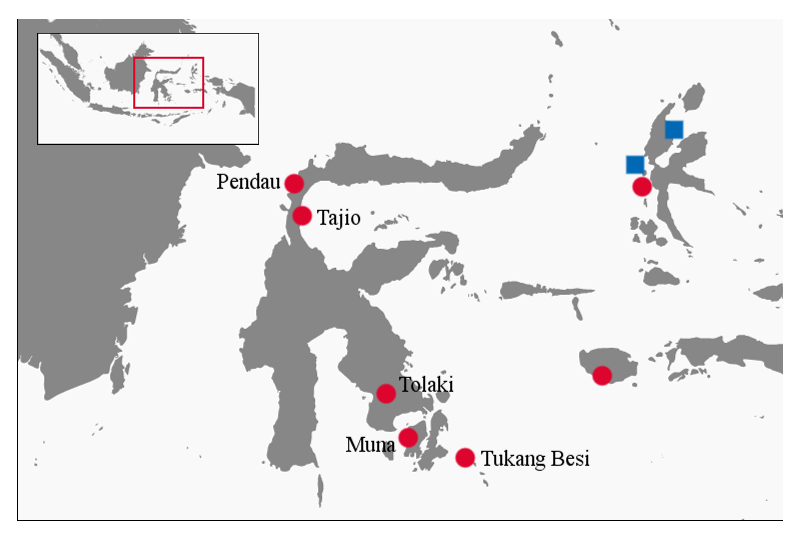
\includegraphics[width=0.7\textwidth]{figures/Map_Sulawesi2.eps}
\caption{Distribution of languages from the Sulawesi subarea.}\label{map:Sul}

\end{figure}

Typologically, both languages belong to Himmelmann's symmetrical voice-languages and display a range of Philippine-type features, the most prominent one being a symmetrical voice system with two basic transitive constructions, each marked by overt morphology. Both Pendau and Tajio differentiate between an actor and an undergoer voice construction. In Pendau, the grammatical subject (or pivot\footnote{As the NP sensitive to a given grammatical process is more cautiously called by most research on subjects in Philippine-type systems.}) is defined by position in the preverbal slot, as Quick shows \citep[124]{Quick2007}. If the undergoer argument becomes the pivot in an undergoer voice construction, the NP is moved into preverbal position in order to be marked as pivot. Explicit verbal morphology on the verb specifies the pivot as being the undergoer.

\ea 
\langinfo{Pendau}{Austronesian, WMP}{\citealt[124]{Quick2007}}\\
\ea \label{Pendau_ex1}
\gllll siama'u nonuju siina'u \\
si=ama='u N-pong-tuju si=ina='u \\
 \textsc{nm}=father=\textsc{1}\textsc{sg}.\textsc{gen} \textsc{rls}-\textsc{sf}-send \textsc{nm}=mother=\textsc{1}\textsc{sg}.\textsc{gen} \\
 \textbf{Pivot=A} {} \textbf{Non-pivot=P} \\
\glft `MY FATHER sent my mother.' \\ 
\ex \label{Pendau_ex2}
\gllll siama'u nituju niina'u \\
si=ama='u ni-tuju ni=ina='u \\
 \textsc{nm}=father=\textsc{1}\textsc{sg}.\textsc{gen} \textsc{iv}.\textsc{rls}-send \textsc{nm}.\textsc{gen}=mother=\textsc{1}\textsc{sg}.\textsc{gen} \\
 \textbf{Pivot=B} {} \textbf{Non-pivot=A} \\
\glft `My mother sent MY FATHER.'\\ 
\z
\z

In (\ref{Pendau_ex1}), the argument \textit{siama'u} receives an actor interpretation whereas in (\ref{Pendau_ex2}), it is assigned the undergoer role by virtue of the undergoer voice formative on the verb.\footnote{Note that Quick argues for this system to be a pragmatic inverse system on a par with inverse systems found, for instance, in some North American languages. Whatever the advantages for such an analysis may be, the Pendau system is in essence one variant of a symmetrical voice system. Both voice constructions are equally basic in terms of morphological marking as well as in terms of frequency (the \textit{ni}-construction was about 20\% more frequent in Quick's analyses, \citealt[580]{Quick2007}). The term inverse, however, implies that some system is flipped from its normal state to a marked/unnormal one. As this is clearly not what proponents of the symmetrical voice approach want to state about voice systems of this type, I will treat the Pendau system as an ``ordinary" symmetrical voice system.} A further parameter in this construction pair is constituent order alternation. For both the \textit{nong}- and the \textit{ni}-construction there is also a predicate-initial order of constituents available: A \textit{nong}-V O may be replaced by \textit{nong}-V O A, and O \textit{ni}-V A can give way to an alternative order \textit{ni}-V A O \citep[366]{Quick2007}.\footnote{Here and in the remainder of the book, I will use the generalised role labels as introduced by \textcite{Dixon1979} and recently summarised by \textcite{Bickel2011}: S -- sole argument of an intransitive verb, A -- most actor-like argument in a transitive verb, O -- not most actor-like argument in a transitive verb, T -- most patient-like argument in a ditransitive construction, and G -- most goal-like or ground-like argument in a ditransitive construction (see \citealt[402ff.]{Bickel2011}).}

Another feature of Pendau (and Tajio) that is shown by the examples above is that the verbs do not carry any person-marking morphology that would cross-reference the arguments with the syntactic functions of the clause. The verb stem does take a lot of formatives at times, basically stem-forming morphology and valency-increasing applicatives and causatives, yet there is no direct link established to the NPs in the clausal context other than by position in the clause (as well as through subtle variation in the assigment of the nominal markers, note for instance the switch from absolute case to genitive case in the actor argument in (\ref{Pendau_ex2})). The Tajio voice system works in a quite similar way, and shows related formatives \textit{noN-/moN-} for actor voice realis/non-realis, and \textit{ni-/nu-} for undergoer voice realis/non-realis (see \citealt{mayani2013grammar} for further details). 

Notably, serial verb constructions are mostly confined to cases where uninflectible directional verbs interact with voice-marked verbs. A first example for illustration is given below in (\ref{tajio01}) from Tajio.

\ea \label{tajio01}
\langinfo{Tajio}{Austronesian, WMP}{\citealt[289]{mayani2013grammar}}\\
\glll sia’u jiopo mai nendiis \\
sia’u jio=po mai ne-ndiis \\
 \textsc{1}\textsc{sg} \textsc{neg}=\textsc{cont} go.to \textsc{dyn}.\textsc{rls}-bath\\
\glft ‘I have not gone for a bath yet.’\\ 
\z

Tolaki, Muna, and Tukang Besi form the second group of Sulawesi languages in the sample. They are all spoken in the far south-east of Sulawesi. While the Tolaki community is located on the tip of mainland Southeast Sulawesi, the Muna and Tukang Besi speaking communities live on islands located off the mainland (Muna and Buton are larger islands close to the coast, while the Tukang Besi islands are smaller coral islands forming a chain out into the Banda sea). 

In contrast to Pendau and Tajio, all three Southeastern Sulawesi languages make use of argument indexing systems where pronominal affixes or clitics on the verb crossreference NP arguments in the clause. In Tolaki, both subjects and objects in transitive clauses are crossreferenced by two sets of clitics on the verb. In intransitive clauses, the S argument may receive marking from either class, rendering Tolaki subject crossreferencing a fluid-S system \citep[115]{mead2008verb}. Example (\ref{tolaki1}) below shows a transitive clause with a prononimal subject argument and a full NP object that is crossreferenced by the suffix on the verb. Note that certain clause-initial monosyllabic function words may attract the subject clitic, drawing it off the verb.

\ea \label{tolaki1}
\langinfo{Tolaki}{Austronesian, WMP}{\citealt[114]{mead2008verb}}\\
\gll a-no wohiki-'i ana-ndo \\
and-\textsc{3}\textsc{sg}.\textsc{nom} wash-\textsc{3}\textsc{sg}.\textsc{abs} child-\textsc{1}\textsc{pl}.\textsc{in}.\textsc{gen} \\
\glft `...and he washed our child.'\\ 
\z

Tukang Besi has developed a similar system of pronominal subject and object indexing on the verb, yet showing an intricate interplay with case-marking articles of the (pro)nominal arguments in the clause. The basic unmarked transitive construction involves both subject and object indexing on the verb. The O argument follows in postverbal position and is marked with the nominative article \textit{na}, the A argument comes last and is assigned the core article \textit{te} (cp. example (\ref{tukbes1a}) below). If the pronominal object indexer on the verb is left out, however, the case-marking system shows the reverse pattern: now the O argument receives the core case marker \textit{te}, while the A argument is coded as nominative by \textit{na} (as in (\ref{tukbes1b})). \citet[53]{donohue1999} analysed this system as some kind of Philippine-type voice system, though he pointed out that the ``normal transitive" construction is the one with pronominal object indexing, accounting for about 70\% of the forms found in texts and being in fact the only choice for some verbs. Therefore, the Tukang Besi voice system does not match the characteristics of the symmetrical voice systems found elsewhere in Sulawesi. The pair of examples in (\ref{tukbes11}) illustrates the switch pattern.

\ea \label{tukbes11} 
\langinfo{Tukang Besi}{Austronesian, WMP}{\citealt[53]{donohue1999}}\\
\ea \label{tukbes1a}
\gll no-kiki'i-ko (na iko'o) te beka \\
\textsc{3}.\textsc{rls}-bite-\textsc{2}\textsc{sg}.\textsc{obj} \textsc{nom} \textsc{2}\textsc{sg} \textsc{core} cat \\
\glft `The cat bit you.' \\ 
\ex \label{tukbes1b}
\gla no-kiki'i te iko'o na beka \\ 
\textsc{3}.\textsc{rls}-bite \textsc{core} \textsc{2}\textsc{sg} \textsc{nom} cat \\
\glft `The cat bit you.'\\ 
\z
\z

The Muna inflectional system is a bit different again. Subject indexing is expressed via three classes of subject prefixes, basically dividing the Muna verbs into three classes: dynamic intransitive verbs mostly take class I prefixes, transitive verbs take class II prefixes, and stative intransitives take class III, albeit with exceptions. Object inflection, on the other hand, is not a crossreference system but involves pronominals attached as suffixes to the verb. Examples (\ref{muna1a}) and (\ref{muna1b}) illustrate a pair of transitive clauses. In the first clause, an NP object does not trigger object inflection on the verb, while a pronominal object in the second case does. A further interesting feature of class II prefixes is the so-called definiteness shift that occurs with definite objects. If the object is definite, the class II prefix on the verb shifts to a class I prefix (in the example, the shift is from \textit{ne-} to \textit{no-}).

\ea 
\langinfo{Muna}{Austronesian, WMP}{\citealt[65]{vandenberg1989}}\\
\ea \label{muna1a}
\gll ne-pepe-mo se-mie \\
\textsc{3}\textsc{sg}.\textsc{rls}-hit-\textsc{prfv} one-person \\
\glft `He hit somebody.' \\ 
\ex \label{muna1b}
\gll no-pepe-kanau-mo \\ 
\textsc{3}\textsc{sg}.\textsc{rls}-hit-me-\textsc{prfv} \\
\glft `He hit me.' \\ 
\z
\z

Other typical Sulawesi features that occur in all five languages include a bipartite mood marking system on the verb, assigning realis or irrealis mood either through variation of the nasal segment in verbal prefixes, or through changes in the vowel quality of subject agreement prefixes. A further conspicuous feature of most Sulawesi languages is the system of aspectual enclitics attached to the verb. These clitics come in two shapes \textit{=nV/=mV} and \textit{=pV}, the former denoting perfective `already'-type semantics, the latter one denoting continuative `still'-type semantics (example (\ref{muna1a}) above illustrates the former aspectual in Muna). The placement of these aspectuals poses an interesting challenge to the delimitation of multi-verb sequences as they are sometimes attracted to the first verb, and sometimes to the last one, possibly reflecting underlying constructional differences. \tabref{table:overviewsulawesi} sums up the main verbal features of the five Sulawesi languages.

\begin{table}
\resizebox{\textwidth}{!}{\begin{tabular}{l r r r}
\lsptoprule
language & constituent order & argument indexing & other verbal inflection \tabularnewline
\midrule
Pendau & SV, AVO & -- & voice, mood \tabularnewline
Tajio & SV, AVO/VOA & -- & voice, mood \tabularnewline
\midrule
Muna & VS, AVO & S/A crossref & mood \tabularnewline
Tolaki & SV, AVO? & S/A, O crossref & -- \tabularnewline
Tukang Besi & VS, VAO & S/A, O crossref & mood \tabularnewline
\lspbottomrule
\end{tabular}}
\caption[Basic verbal features of the Sulawesi languages]{Overview of basic verbal features of the Sulawesi languages in the data set. Constituent order lists only the basic pattern, pragmatically induced alternative patterns are often also available.}
\label{table:overviewsulawesi}
\end{table}

\subsection{Nusa Tenggara} \label{sec:nus}

Where the languages of Sulawesi put most informational load on the verbal head of the clause, for instance by argument indexing formatives, stem-forming morphology, voice and mood markers, the languages of Nusa Tenggara show only limited verbal morphology. Moving from west to east, we can see that Kambera still retains a rich person marking system on the verb, while the Papuan languages of Alor and Pantar only occasionally show verbal person marking, and the Austronesian languages Alorese and \ili{Waima'a} have lost all verbal morphology and have developed towards highly isolating languages.

\begin{figure}

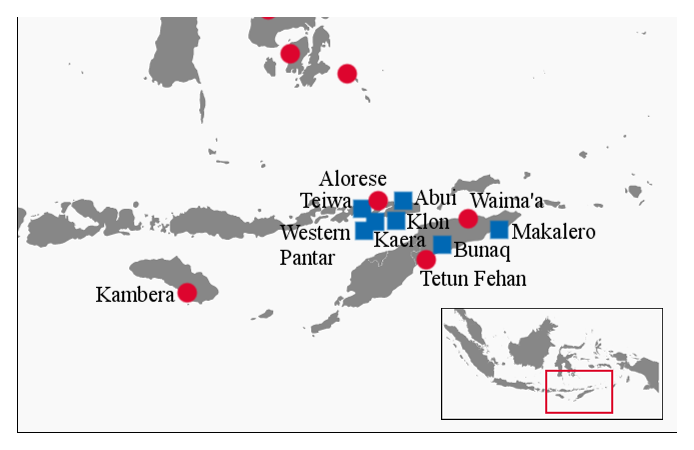
\includegraphics[width=0.7\textwidth]{figures/Map_Nusa2.eps}
\caption{Distribution of languages from the Nusa Tenggara subarea.}\label{map:Nus}

\end{figure}  

The Austronesian language Kambera is spoken on the island of Sumba, located south of the Sunda-Banda island chain. Kambera is the westernmost language of the Lesser Sunda islands that has been included in the sample (cf. \figref{map:Nus}), and presents some features that are more reminiscent of Western Austronesian languages than of the languages of Eastern Indonesia. The verb system features four sets of pronominal clitics, each marking one of the ``cases" nominative, genitive, accusative, and dative. The crossreferencing system in Kambera is sensitive to certain clitic sequences and to definiteness in NPs, both of which may influence the clitic choice and combination on the verb. Example (\ref{kamb1a}) shows a canonical transitive construction. Both NP arguments are optional as their properties are coded by clitics on the verb. The next two examples in (\ref{kamb1b}) and (\ref{kamb1c}) illustrate two situations which prohibit crossreferencing of all three arguments on the verb. In (\ref{kamb1b}), the sequence of two third person objects causes the direct object clitic to be omitted. In (\ref{kamb1c}), the direct object also fails to be crossreferenced on the verb because it is indefinite.

\ea 
\langinfo{Kambera}{Austronesian, CMP}{\citealt[63f.]{klamer1998grammar}}\\
\ea \label{kamb1a}
\gll (na tau wútu) na-palu-ka (nyungga) \\
\textsc{art} person be.fat \textsc{3}\textsc{sg}.\textsc{nom}-hit-\textsc{1}\textsc{sg}.\textsc{acc} I \\
\glft `The big man hit me.' \\ 
\ex \label{kamb1b}
\gll I Ama na-wua-nja$_k$ [na heu na njara]$_j$. \\
\textsc{art} father \textsc{3}\textsc{sg}.\textsc{nom}-give-\textsc{3}\textsc{pl}.\textsc{dat} \textsc{art} one.\textsc{clf} \textsc{art} horse \\
\glft `Father gives them one horse.' \\ 
\ex \label{kamb1c}
\gll (I Ama) na-kei-nja rí. \\ 
\textsc{art} father \textsc{3}\textsc{sg}.\textsc{nom}-buy-\textsc{3}\textsc{pl}.\textsc{dat} vegetable \\
\glft `Father buys them vegetables.'\\ 
\z
\z

A further conspicuous feature of Kambera is the presence of overtly marked subordinating constructions: a verbal prefix explicitly marks controlled clauses as well as nominalised/relativised subordinate clauses. Overt subordination strat\-e\-gies such as these replace certain types of \textsc{multi-verb construction}s, and set Kambera apart from all other languages in the data set.\footnote{A putative further case where a language might be analysed as having non-finite morphology is the \textit{-um-} infix in Tolaki. However, the occurrence of \textit{-um-} is dependent upon a range of phonological, morphological, syntactic and pragmatic factors, rendering it an unstable indicator for non-finiteness. The data are further complicated by the existence of a homophonous \textit{-um-} morpheme that appears to mark repetitive action in manner of motion verbs. See \citet[117]{mead2008verb} for further discussion.} The following examples illustrate the use of overtly marked subordination in Kambera. Example (\ref{kamb2a}) shows a combination of a nominalised subordinate clause that is linked to the direct object of the matrix clause via the relativiser \textit{pa-}. In (\ref{kamb2b}), the subordinate clause is marked as a controlled clause by a homophonous \textit{pa-}, indicating that the subject of the matrix clause controls the subject of the embedded clause.

\ea 
\langinfo{Kambera}{Austronesian, CMP}{\citealt[338]{klamer1998grammar}}\\
\ea \label{kamb2a}
\gll ta-pakiri-nya$_j$ $[$na pa-tinu-nda$]_{\textsc{np} \textit{j}}$ \\
\textsc{1}\textsc{sg}.\textsc{nom}-start-\textsc{3}\textsc{sg}.\textsc{dat} \textsc{art} \textsc{rel}-weave-\textsc{1}\textsc{sg}.\textsc{dat} \\
\glft `We start (with) (it) our weaving.' \\ 
\ex \label{kamb2b}
\gll ta-pakiring $[$pa-tinu-nya na lau haromu$]$ \\ 
\textsc{1}\textsc{sg}.\textsc{nom}-start \textsc{ctr}-weave--\textsc{3}\textsc{sg}.\textsc{dat} \textsc{art} sarong tomorrow \\
\glft `We start weaving/to weave the sarong tomorrow.'\\ 
\z
\z

The other Nusa Tenggara languages of the sample are markedly different from the Kambera type. Most of these languages are characterised by two tendencies. First, there is a (massive) reduction in verbal morphology (including person-marking clitics), leading to languages with little or no verbal formatives. And second, if inflection on the verbs is retained, we often find irregular inflection patterns. 

If verbal inflection is present, the languages typically exhibit person-marking prefixes or clitics. The Papuan languages show some variation with regard to the number of person-marking paradigms. \citet{schapper2014intro} reports that West Alor languages typically have three paradigms, east Alor languages two paradigms, and Pantar languages only one paradigm. In terms of verb morphology, we may group the remaining Nusa Tenggara languages in the sample into two classes. First, languages that show regular argument indexing in some category, or retain part of their indexing system although the system is not completely obligatory and omission of person-markers is triggered by grammatical or lexical factors: this applies to Abui, Teiwa, Klon, Bunaq, Western Pantar, and Kaera. And second, languages that have either lost their verb morphology completely or still display remnants of person-marking, but only under specific phonological or lexical conditions. This pertains to Makalero, Tetun Fehan, Alorese, and \ili{Waima'a}, with the former two showing residual marking patterns, and the latter two being (almost) completely isolating. All three Austronesian languages go in this second group. For the Papuan TAP languages, \textcite{klamer2012development} summarise the number of person-marking paradigms and the alignment system. Here, I only show those languages that are in the sample.

\begin{table}
\begin{tabular}{l l r l}
\lsptoprule
island & language & no. of prefix paradigms & alignment \tabularnewline
\midrule
Pantar & Western Pantar & 1 & split-S \tabularnewline
 & Teiwa & 1 & accusative \tabularnewline
 & Kaera & 3 (1) & accusative \tabularnewline
 Alor & Klon & 3 & split-S \tabularnewline
 & Abui & 5 & split-S \tabularnewline
 Timor & Bunaq & 1 & accusative \tabularnewline
 & Makalero & (1) & (accusative) \tabularnewline
\lspbottomrule
\end{tabular}
\caption[Overview of TAP prefix paradigms and alignment types]{Overview of TAP prefix paradigms and alignment types (taken from \citealt[178]{klamer2012development}), the Kaera data were added from \citet[128]{klamer2014kaera}.}
\label{table:TAPprefixalign}
\end{table}

Abui is the language with the most abundant verb morphology in the TAP group. Abui has both person-marking prefixes and aspectual suffixes on the verb, showing more formative load on the clausal head than is found in most of the other TAP languages. As in other Papuan languages of the area, it is only undergoer arguments that may be crossreferenced by bound pronouns on the verb. A arguments are always expressed by free forms. A feature that seems quite common in the Nusa Tenggara area is that the person-marking systems found on the verbs regularily interact with certain properties of the crossreferenced argument. We have already seen that in Kambera indefinite arguments fail to attract a crossreferencing clitic on the verb. This is mirrored in Abui and other TAP languages by similar interaction mechanisms. In Abui, person-marking is found to be sensitive to contrasts in specificity. For instance, the two object referents in (\ref{abui1a}) and (\ref{abui1b}) evoke different crossreferencing patterns. While the amount of wood is non-specific in the first clause and thus no clitic appears on the verb, it is given a specific reading in the second clause by means of the undergoer clitic.\footnote{Class II clitics are referred to as ``locatives" by Kratochvíl, and comprise ``prototypical locations, including the
benefactives and malefactives (human location), theme (location of the event), and
purpose (location in time)" \citep[188]{kratochvil2007grammar}. Argument indexing in Abui thus includes a range of non-prototypical core arguments exceeding the number of argument roles that are reported to be indexed in other TAP languages.}

\ea
\langinfo{Abui}{Papuan, TAP}{\citealt[179]{kratochvil2007grammar}}\\
\ea \label{abui1a}
\gll maama bataa fak-d-a \\
father wood break-hold-\textsc{dur} \\
\glft `Father splits wood.’ \\ 
\ex \label{abui1b}
\gll maama bataa he-fak-d-a \\ 
father wood \textsc{3}II.\textsc{loc}-break-hold-\textsc{dur} \\
\glft `Father splits the wood. (the nearer defined quantity of wood)’\\ 
\z
\z

Two further characteristics of the Abui grammar become apparent in the example pair above. First, there is a set of aspectual suffixes that attach to the verb. These suffixes are not obligatory in the sense that every verb has to have one. Yet if a verb takes one, there is a constraint concerning the stem allomorph of the verb: Verbs in Abui show stem alternations. These alternations affect the coda and express either completive (final boundary), continuative (no boundary) or inceptive events (initial boundary). That is, aspectual encoding in Abui is at least distributed across two different grammatical layers. Second, according to Kratochvíl's analysis, Abui not only has a great wealth of serial-verb constructions at the syntax level, but also another layer of verb combination, which he names complex verb (formation). Just like \textit{fak} `break' and \textit{d} `hold' are argued to yield \textit{fak-d} `split' in (\ref{abui1a}), verbal roots are often presented in compounds and seem to interact in non-trivial ways with verb combinations at the the syntactic layer. This complexity in verb formation would be quite exceptional (reminiscent of the Kalam verb system), and appears to be completely unparalleled in both AP languages as well as in the other languages of Easten Indonesia. In fact, there have been doubts that Abui verb roots can indeed be decomposed in such ways (Antoinette Schapper, p.c.;  comments from an anonymous reviewer). Therefore, and in order to enhance readability, I will paraphrase all complex verb roots in Abui by leaving the verb compound intact and glossing it the way the free translation suggests. In the above examples, for instance, the verb would read \textit{fakd-} and be glossed as `split', just as indicated by the free translation.

Turning to the other languages in this group, we find that, for instance, Western Pantar has a single set of argument indexing prefixes that are obligatory with one (small) set of verbs, optional with another (the majority), and illicit with still other verbs (basically stative intransitives, \citealt[76]{holton2014western}). Depending on the verb, the prefix may either denote an undergoer argument (O or G), or, in some cases, two prefixes occur in sequence with the first one marking the A argument and the second one the O argument, as in (\ref{wp01}). NP arguments may optionally stand in apposition to a person-marking prefix (cp. (\ref{wp02a})), but may also be dropped. The person-marking system is sensitive to contrasts in animacy. If the undergoer referent is inanimate, no co-referential pronoun may occur next to the bound prefix on the verb (\ref{wp02b}).

\ea \label{wp01}
\langinfo{Western Pantar}{Papuan, TAP}{\citealt[77]{holton2014western}}\\
\gll ke'e pi-ga-ussar \\
fish \textsc{1}\textsc{pl}.\textsc{in}-\textsc{3}\textsc{sg}-catch \\
\glft `We are catching fish.'\\ 
\z

\ea
\langinfo{Western Pantar}{Papuan, TAP}{\citealt[77]{holton2014western}}\\
\ea \label{wp02a}
\gll nang bla ga-niaka \\
\textsc{1}\textsc{sg}.\textsc{act} house \textsc{3}\textsc{sg}-see \\
\glft `I saw the house.' \\ 
\ex \label{wp02b}
\gll *nang gaing ga-niaka \\ 
\textsc{1}\textsc{sg}.\textsc{act} \textsc{3}\textsc{sg}.\textsc{ug} \textsc{3}\textsc{sg}-see \\
\z
\z

Kaera, a neighbour to Western Pantar and Teiwa on Pantar island, has a similar indexing system. Transitive verbs in Kaera fall into three classes which either always take a person-marker to encode O, or optionally take a person-marker, or never express O with a prefix but only with a free NP. This pattern looks quite like the Western Pantar system in that it depends on the verb lexeme whether or not a prefix is required. Interestingly, however, among the smallish class of five verbs in Western Pantar that obligatorily trigger indexing are two verbs, \textit{-niaka} `see' and \textit{-kkang} `hit' \citep[77]{holton2014western}, the equivalents of which in Kaera belong just to the opposite class: \textit{lal-} `see' and \textit{kup-} `hit (thing, person)' refuse bound O-constituents on the verb. 

The suffix slot in Kaera may either be filled with a marker of clause-final position, or with one of three aspectual suffixes. The phonological shape of the verb root determines whether or not the clause-final marker \textit{-o} is attached. Example (\ref{kaera1}) shows two clauses. In the first clause, the verb receives the clause-final marker due to its position at the end of the clause. In the second clause, the verb is followed by an aspectual and therefore not marked with \textit{-o}, but instead occurs with one of the aspectual suffixes that are restricted to verbs in non-final position.

\ea \label{kaera1}
\langinfo{Kaera}{Papuan, TAP}{\citealt[142]{klamer2014kaera}} \\
\ea
\gll ging tei gu patak-o \\
\textsc{3}\textsc{pl} tree that cut-\textsc{fin} \\
\glft `They cut that wood.' \\ 
\ex
\gll ging tei gu patak-i sei \\ 
\textsc{3}\textsc{pl} tree that cut-\textsc{prfv} \textsc{compl} \\
\glft `They have cut that wood.'\\ 
\z
\z

Klon, Teiwa, and Bunaq basically all show variations of these patterns. Teiwa indexes animate O arguments with prefixes on the verb, and has a reduced reality status inflection consisting of just one morpheme, \textit{-Vn}. It marks ``whether an event has been realized (`realis status') or not (`irrealis status')" \citep[245]{klamer2010grammar}. The latter is zero marked in Teiwa. As the difference between a zero-marked irrealis and a potential bare verb cannot be determined from the published data, this feature causes serious problems in interpreting whether a given verb in a MVC is in fact inflected (through zero-marking) or not. S encoding in intransitive clauses is more straightforward in Teiwa than in other TAP languages: There is no semantic alignment, and the subject of unaccusative clauses is formally marked just the way subjects of unergative clauses are \citep[169]{klamer2010grammar}. Klon, on the other hand, does have a semantic alignment system showing the familiar subcategorisation into obligatory and optional O indexing verbs. Some intransitive verbs always take an actor argument, some always take an undergoer argument, and some verbs can take either. According to Baird, alignment choice in Klon is effected by the parameters performance, effect, instigation, control, and affectedness \citep[52]{baird2008grammar}. Among the group of alternating intransitives, we find for instance that \textit{g-emeq} (\textsc{3ug.I}-not.want) means `she (inherently) doesn't want' while \textit{ga emeq} (\textsc{3sg.act} not.want) translates as `she (decidedly) doesn't want'. Bunaq essentially shows the same argument indexing system as in Western Pantar. Animate O arguments are indexed on the verb by a set of prefixes while inanimate Os are not. 

We can see from the range of different indexing systems in TAP languages, as well as from their irregular patterns, that the general diachronic development in these languages is directed towards a reduction of verbal morphology. Verbal inflection, be it argument indexing morphology, aspect morphemes or other formatives, can therefore not be regarded as obligatory anymore. As already indicated for Teiwa, this has repercussions for MVC analysis inasmuch as inflection is certainly not a constructional property. Its occurrence is in many cases too scant for any analysis trying to determine which verb is the ``main verb" in a given construction. This trend to inflection reduction accords well with the second, still more isolating group of languages in Nusa Tenggara.\footnote{Note that verbal morphology has been reconstructed for both Papuan TNG languages and Malayo-Polynesian languages. Although readers that are less familiar with the area might wonder whether absence of inflection in the Timor area could not be regarded as an ancient feature, the diachronic context into which the languages have been placed rather suggests a gradual erosion of inflection.} Here we can observe a later stage: the indexing systems as well as all other morphology is already on its way to being completely lost. \ili{Waima'a} can be considered the isolating endpoint of this morphological breakdown. \ili{Waima'a} does not have an indexing system on the verb, yet there is still verbal reduplication and a (partially productive) causative prefix \textit{ra-}. \ili{Waima'a} shows the basic Austronesian clausal syntax, having SV/AVO word order (with other orders being also quite common) and accusative alignment. Both S, A and O arguments are frequently elided if they are retrievable from context \citep{bowden2006}. For instance, in a context where fire making is already an established topic, the following utterance with elided O can be regarded unmarked:

\ea 
\langinfo{Waima'a}{Austronesian, CMP}{\citealt[29]{bowden2006}}\\
\gll mai buni aku loo \\
come look \textsc{1}\textsc{sg} make \\
\glft ‘Come and see me make (fire).’
\z

Tetun Fehan and Alorese are quite similar to \ili{Waima'a}. They also show Austronesian SV/AVO constituent order and accusative alignment. Their argument indexing system, however, is still extant, being reduced to a class of phonologically defined verbs. In Alorese, only a handful of vowel-initial verbs still display argument indexing of the A argument (not O, as in the TAP languages). Furthermore, the verb `eat' in Alorese is irregular and shows suppletion between \textit{(g)Vng} and \textit{-aka} \citep[61]{klamer2011alorese}. In Tetun Fehan, an Austronesian language spoken on Timor (Fehan is one of the western Timorese Tetun dialects), we find just the reverse pattern: here, vowel-initial verbs do not index the subject anymore, while h-initial verbs still retain a paradigm covering singular persons and 3PL,\footnote{\citet[173 footnote 5]{vanklinken1999grammar} notes that the missing subject markers for first and second person plural in Tetun Fehan have to be considered a diachronic loss as the reconstructed system of Proto Central Malayo-Polynesian has them, as well as neighbouring languages \ili{Dawan} and \ili{Rotinese}.} and consonant-initial verbs still take the indexer \textit{k-} for first person singular, but no other markers. Subject indexing in Tetun Fehan is a regular process, NP expression is optional and ellipsis of both subjects and objects is as common as in \ili{Waima'a}. There is a further interesting difference between subject indexing on h-initial verbs and consonant-initial verbs. It is only h-initial verbs that all take subject marking in a verb series, while C-initial verbs in a series only inflect in V$_1$ position. Compare the following two examples from \citet{vanklinken1999grammar}. In the first verb string in (\ref{tetun01}) the verbs \textit{halai}, \textit{hola} and \textit{hikar} all take the subject indexer \textit{n-} for third person. In (\ref{tetun02}), on the other hand, both verbs begin with a consonant other than h which is why the second verb, \textit{nono}, does not take the person marker here.

\ea \label{tetun01}
\langinfo{Tetun Fehan}{Austronesian, CMP}{\citealt[174]{vanklinken1999grammar}}\\
\gll sia n-alai onan, n-alai n-ola n-ikar loro-sa'e-n bá \\
\textsc{3}\textsc{pl} \textsc{3}-run \textsc{imm} \textsc{3}-run \textsc{3}-take/via \textsc{3}-back sun-ascend-\textsc{gen} go \\
\glft `They ran, ran away further to the east.'
\z

\ea \label{tetun02}
\langinfo{Tetun Fehan}{Austronesian, CMP}{\citealt[175]{vanklinken1999grammar}}\\
%\begingl
%\rightcomment{{\small \textbf{Tetun Fehan} \textsc{nus}}}
\gll ha'u k-bá nono wé á \\
\textsc{1}\textsc{sg} \textsc{1}\textsc{sg}-go heat(.liquid) water \textsc{def} \\
\glft `I went and boiled water...'
\z

The last language of the Nusa Tenggara group to be introduced here is Makalero, another one of the four Papuan languages spoken on Timor. Makalero is largely isolating with very few morphological processes on the verb. The only person marking device that still exists in Makalero is the formative \textit{k-} that occurs with a smallish set of vowel-initial verbs and encodes O arguments. Example (\ref{Makal}) illustrates the use of \textit{k-}.

\ea \label{Makal}
\langinfo{Makalero}{Papuan, TAP}{\citealt[253]{huber2011}}\\
\gll nana pere=ni muni k-afu=ni mu’a-ia-la’a \\
snake big.\textsc{sg}=\textsc{lnk} return \textsc{3}.\textsc{ug}-carry=\textsc{lnk} ground-under:\textsc{red}-move \\
\glft `...having become a large snake, he carried her under the earth.’ 
\z

The distinction between bound pronominal \textit{k-} and the free pronoun forms, however, is blurred in Makalero as the pronouns may also occupy the pre-verbal ``complement" slot, apparently behaving like prefixes (at least this is suggested by Huber's transcription). Compare the following example where \textit{ani} `1SG' appears to be prefixed to the verb \textit{uta} `kill'.

\ea \label{makalero2}
\langinfo{Makalero}{Papuan, TAP}{\citealt[350]{huber2011}}\\
\gll ei=ni ani mei pa’uk-ini=si ani-uta=si \\
\textsc{2}\textsc{sg}=\textsc{contr} \textsc{1}\textsc{sg} take bad-do:\textsc{bd}=\textsc{lnk} \textsc{1}\textsc{sg}-kill=\textsc{lnk} \\
\glft `It was you who destroyed me and killed me.’ 
\z

A further exceptional feature of Makalero is a constraint on verbs against taking more than two arguments. Ditransitive configurations are resolved by making use of the light verb \textit{mei} (developed from \textit{mei} `take'), as can be seen in example (\ref{makalero2}). Because the second argument slot of the verb \textit{ini} `do' is already occupied by the modifier \textit{pa'uk} `bad' (the pre-verbal complement slot triggers the use of a bound verb form, glossed with \textsc{bd}) \textit{mei} takes over the role of the object-licensing verb, and the construction is literally speaking a trivalent `you do me bad' with `bad' acting as some kind of argument.

Summing up, we can see that the wealth of verbal morphology found in the Sulawesi languages gives way to more reduced verb systems in the Nusa Tenggara area with a marked decline of person-marking systems from west to east, culminating in highly isolating languages such as \ili{Waima'a} on Timor. Both the Papuan and Austronesian languages in the area largely retain their inherited features in the clausal domain. For instance, while the Austronesian languages have SV/AVO word order, the Papuan languages are verb-final languages. A further genealogical trend can be found in the person-marking systems. Papuan languages tend to mark undergoer arguments, while Austronesian languages tend to index the actor argument on the verb. \tabref{table:overviewnusa} summarises the main verbal features of the area.

\begin{table}[h]
\resizebox{\textwidth}{!}{\begin{tabular}{l r r r}
\lsptoprule
language & constituent order & person marking & other verbal inflection \tabularnewline
\midrule
Kambera & SV, AVO & (S/A,O[+def]) & -- \tabularnewline
Abui & SV, AOV & (O[+spec]) & aspect \tabularnewline
Western Pantar & SV, AOV & (O,G,(A)) & -- \tabularnewline
Kaera & SV, AOV & (O) & aspect, final \tabularnewline
Teiwa & SV, AOV & (O[+an]) & ``reality status" \tabularnewline
Klon & SV, AOV & (S$_O$, O) & -- \tabularnewline
Bunaq & SV, AOV & (S$_O$, O[+an]) & -- \tabularnewline
\ili{Waima'a} & SV, AVO & -- & -- \tabularnewline
Alorese & SV, AVO & (A) & -- \tabularnewline
Tetun Fehan & SV, AVO & (S/A) & -- \tabularnewline
Makalero & SV, AOV & (O) & -- \tabularnewline
\lspbottomrule
\end{tabular}}
\caption[Basic verbal features of Nusa Tenggara languages]{Overview of basic verbal features of the Nusa Tenggara languages in the EI data set. Constituent order lists only the basic pattern, pragmatically induced alternative patterns are often also possible. Brackets around person marking formulae indicate that the system does not apply to all verbs in all contexts. Grouping of languages is roughly according to the discussion in the prose.}
\label{table:overviewnusa}
\end{table}

\subsection{Maluku} \label{sec:maluku}

This language group forms a small sample, consisting of only five languages, three of them Austronesian, and two Papuan. They are all spoken in the Moluccas between the Lesser Sunda Islands and Timor in the southwest, and mainland Papua with the Bird's Head and Bomberai peninsula in the north and east. The Maluku languages come in two typological groups that differ considerably from each other. The southern group consists of Selaru and Buru, each spoken on one of the many islands between Timor and mainland Papua. The northern group is located on and off the island of Halmahera in the northern Moluccas (see \figref{map:Mal} below).

\begin{figure}

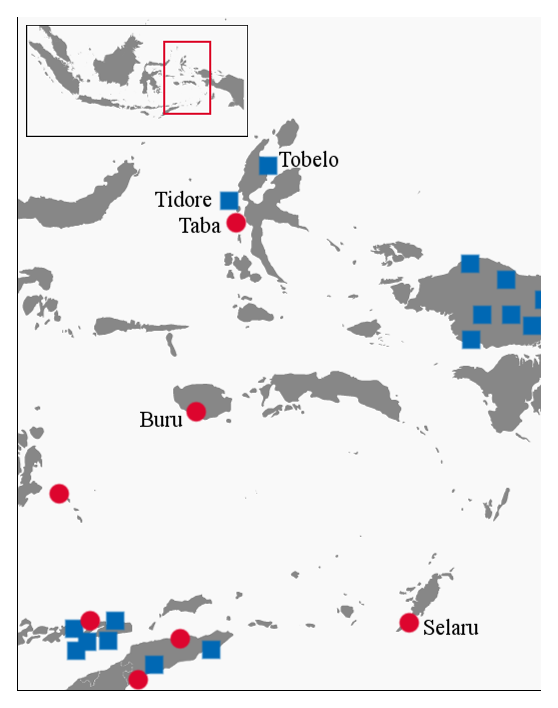
\includegraphics[width=0.55\textwidth]{figures/Map_Maluku2.eps}
\caption{Geographical distribution of languages from the Maluku subarea.}\label{map:Mal}

\end{figure}

Selaru is an Austronesian CMP language with typical SV/AVO constituent order, prepositions and subject indexing by prefixes on the verb. Subject indexing is a regular process and each verb is marked by one of three inflectional classes. The choice is triggered by the stem onset. As in many of the TAP languages, animacy plays a role in Selaru. Inanimate subject referents are crossreferenced on the verb with a special prefix that is neutral with regard to number agreement. Consider example (\ref{selaru1}) below.

\ea \label{selaru1}
\langinfo{Selaru}{Austronesian, CMP}{\citealt[66]{coward2005}}\\
\glll Toto, mbwa ti mal masire ma kele ksyoyeta bakbakare\\
toto, mw-ba ti mw-al masy-Vre ma kele ky-soyeta bakbak-Vre\\
boy, \textsc{2}\textsc{sg}-go \textsc{conj} \textsc{2}\textsc{sg}-get fish-\textsc{pl} \textsc{conj} then \textsc{inan}-replace dry-\textsc{pl} \\
\glft `Boy, you go and get some fish in order to replace the dried ones.‘
\z

While the animate subject is indexed on each of the first two verbs by the second person singular prefix \textit{mw-}, the fish from the second VP is reintroduced as the subject of the following clause by use of the inanimate prefix \textit{ky-}. 

A striking feature of Selaru is that MVCs are infrequent and occur in rather unexpected types. One reason for this is that Selaru employs two semantically unspecific linkers, \textit{ti} and \textit{ma}, both of which appear to be grammaticalised from motion verbs.\footnote{The origin of \textit{ma} seems clear from a vast range of surrounding Austronesian and Papuan languages many of which still show reflexes of a reconstructable motion verb *mai `come' (\citealt{ross2008lexicon} give PAn *maRi, *mai `come', PCEMP *mai `come' and POc *mai, *ma `come'/DIR (towards speaker)'. The origin of \textit{ti} is less clear. In \ili{Waima'a}, there is a motion goal verb \textit{tii} meaning `arrive' or `until' in a temporal sense, and Tetun Fehan has \textit{ti'a} meaning `already' both of which are reminiscent of Indonesian \textit{tiba} `arrive' but I have not come across any proposed reconstruction. Selaru seems to use a verb stem \textit{-ait} for `arrive' \citep[175]{coward2005}.} These linkers appear in most contexts where in other languages of the EI area we would find unmarked verb sequences. Example (\ref{selaru1}) from above illustrates this nicely with the motion-action sequence \textit{mbwa ti mal}. In virtually all other languages such a sequence would be expressed by a plain MVC, yet in Selaru one of the two markers overtly chains the two verbs together. Apart from the low use of MVCs, Selaru is a rather typical representative of an Eastern Indonesian language, showing for instance possessive classification with alienable and inalienable constructions (the former of which marks a further split into edible and non-edible possessums) and object preposing (functionally similar to passive alternations, although there is no real voice distinction in Selaru). 

Buru is in some ways similar to Selaru, including the overall scarcity of MVCs, although \citet{grimes1991buru} reports on a range of MVC types. In contrast to Selaru and the other languages included in the Maluku subsample, Buru has lost all inflecting devices on the verb (while retaining a rather elaborate set of derivational prefixes and suffixes). Buru is therefore, from a verb-morphological perspective, more similar to \ili{Waima'a} and Alorese than it is to Selaru.

The other three languages from the Maluku group are both spoken on Halmahera and surrounding islands. Taba (or East Makian) is another Austronesian language, genealogically belonging to the South Halmahera-West New Guinea branch and showing the by now familiar Austronesian word order pattern SV/ AVO. \citet[144f.]{bowden2001taba} points out that while Taba meets most of the typological expectations connected to word order-correlations in VO languages, it does show some sign of deviation, most prominently from the preposed possessor order that \citet{Himmelmann2005austronesian} argued to be a general trait of Eastern Indonesian (Austronesian) languages (see \sectref{sec:preposed}). Actor arguments are expressed by crossreferencing prefixes on the verb. As Taba has developed a split-S system, this pertains to A and S$_A$ arguments. Undergoer S$_O$ arguments are not subject to verbal indexing though pronominal S$_O$ arguments are placed in postverbal position instead of expected SV. In some MVCs, this split leads to interesting constructions where the participant is marked twice, one time as the actor and one time as the undergoer. Consider the example in (\ref{taba1}).

\ea \label{taba1}
\langinfo{Taba}{Austronesian, SHWNG}{\citealt[300f.]{bowden2001taba}}\\
\glll nwosal máddodang i \\
n=wosal máddodang i \\
\textsc{3}\textsc{sg}=stand be.straight \textsc{3}\textsc{sg} \\
\glft `He's standing up straight.'  
\z

The pronoun \textit{i}, which is optional here, is postposed and thus denotes a S$_O$ argument. It is coreferential with the S$_A$ argument indexed on the first verb. This construction is thus similar to reflexive and middle voice constructions \citep[301]{bowden2001taba}, and is mirrored in Taba by another peculiar construction. Verbs of excretion in Taba not only show an indexed actor argument, but also a set of suffixes that are otherwise completely absent from that language. Compare example (\ref{taba2}).

\ea \label{taba2}
\langinfo{Taba}{Austronesian, SHWNG}{\citealt[196]{bowden2001taba}}\\
\glll Buang nciwi \\
Buang n=sio-i \\
Buang \textsc{3}\textsc{sg}=shit-\textsc{3}\textsc{sg} \\
\glft `Buang shat.' 
\z

Just as in (\ref{taba1}), we see that a single participant receives actor and undergoer encoding at the same time. A similar, albeit distinct, construction is also found in Tobelo, one of the Papuan languages that form the closely related Northeast Halmaheran group.

Tobelo retains many Papuan features, including conservative SV/AOV word order, postpositions, gender (male, female, non-human) and noun markers. Core-arguments are indexed on the verb by two sets of prefixes (called subjective and objective paradigm respectively, see \citealt[38]{holton2003tobelo}). The single argument of active intransitives as well as the A argument of transitives are indexed by the subjective paradigm occupying the initial prefix slot. The single argument of stative intransitives and the O argument of transitives, on the other hand, are marked in the second prefix slot by the objective paradigm. Example (\ref{tobelo1}) illustrates a minimal transitive construction in Tobelo (ellipsis being common for topical arguments).

\ea \label{tobelo1}
\langinfo{Tobelo}{Papuan, NH}{\citealt[39]{holton2003tobelo}}\\
\gll i-hi-goli \\
3-1-bite \\
\glft `It/they bit me.' 
\z

Now, there is a further quirk in Tobelo's active-stative system in that the stative intransitives appear to be encoded just like transitive predicates. While the S$_O$ argument is indexed by the objective paradigm in the second slot, the first slot invariably shows neutral third person singular \textit{i-}, effecting some kind of pseudo-transitive construction. Compare the following example:

\ea 
\langinfo{Tobelo}{Papuan, NH}{\citealt[38]{holton2003tobelo}}\\
\gll i-hi-pehaka \\
3-1-wet \\
\glft `I am wet.'
\z

The Taba excretion construction can be formally differentiated from Tobelo's stative intransitives by the fact that the former shows person and number agreement in both markers, while the latter always has \textsc{3sg.nh} for the actor. What is common to both systems is that the referent appears to lack full control of the situation, which is apparently what is captured by the undergoer marking.

Tobelo has an array of further formatives appearing on the verb, such as applicative, distributive, intensifier morphology as well as a set of aspect suffixes denoting perfective, imperfective, repetitive, durative, and sequential events. These aspect suffixes are not obligatory, and do not form a viewpoint aspect system such as in \ili{Russian}. They may occasionally also attach to host classes other than verbs (for instance to nouns and numerals). This makes Tobelo aspect suffixes category-independent \citep[44]{holton2003tobelo}, which casts doubt on the usefulness of theses suffixes as indicators of finiteness in verbs. 

Tidore, another Papuan language of Halmahera, is morphologically less elaborate than Tobelo. Tidore verbs may take a subject prefix\footnote{In van Staden's grammar on Tidore, this prefix is called ``actor prefix". It appears, however, that clear undergoer verbs such as `fall' or `(be) drunk' also accept the prefix (see for instance example (\ref{Tidore1})). Two distinct person-marking paradigms that would convey differences in semantic roles, as we find in Tobelo, are missing in Tidore. In the examples from Tidore I left the \textsc{act} gloss in place though I do understand the prefix set as agreeing more generally to any argument in subject function.} inflecting for person and number (and partially for gender and animacy). Argument indexing, however, seems to be completely optional, without any apparent change as to wellformedness or sociolectal situation. Based on a small exploratory analysis of 80 turntaking units from one conversation, \citet[79]{vanstaden2000tidore} reports that only about one third of all inflectible main verbs actually take an argument indexer. A verb that stays uninflected may thus be uninflected for two reasons: it may either be uninflected simply by pragmatic choice, or through grammatical restrictions. For instance, in the example pair (\ref{Tidore1}), the second verb \textit{tora} remains uninflected because of constructional constraints. The first verb, on the other hand, is free to accept a person marker or to remain bare.

\ea \label{Tidore1}
\langinfo{Tidore}{Papuan, NH}{\citealt[81]{vanstaden2000tidore}}\\
\ea
\gll ngofa ngge peka tora \\
child 3\textsc{nhum}.there fall go.downwards \\
\glft `The child fell down.’ \\ 
\ex
\gll ngofa ngge yo-peka tora \\ 
child 3\textsc{nhum}.there 3\textsc{nhum}.\textsc{act}-fall go.downwards \\
\glft `The child fell down.’ \\    
\z
\z

\tabref{table:overviewmaluku} summarises some of the core features associated with the verb systems of the Maluku subgroup.

\begin{table}[h]
\resizebox{\textwidth}{!}{\begin{tabular}{l r r r}
\lsptoprule
language & constituent order & argument indexing & other verbal inflection \tabularnewline
\midrule
Buru & SV, AVO & -- & -- \tabularnewline
Selaru & SV, AVO & S/A & -- \tabularnewline
Taba & SV, AVO & S$_A$/A & -- \tabularnewline
Tidore & SV, AVO & (S/A) & -- \tabularnewline
Tobelo & SV, AOV & S$_A$/A, S$_O$/O & aspect? \tabularnewline
\lspbottomrule
\end{tabular}}
\caption[Basic features of Maluku verb systems]{Overview of basic verbal features of the Maluku languages in the EI data set. Constituent order lists only the basic pattern, pragmatically induced alternative patterns are often also available. Brackets indicate optional use of argument indexers.}
\label{table:overviewmaluku}
\end{table}

\subsection{Western Papua}\label{sec:westpapua2}

The last subarea is comprised of the westernmost part of mainland New Guinea: the Bird's Head peninsula down to Bintuni Bay, as well as the islands of Cenderawasih Bay to the east. The Bird's Head is a geographically diverse peninsula, ranging from the vast mangrove swamps in the Bintuni Bay area to the Tamrau and Arfak Mountains towering up in the north and east. The region is home to a couple of Papuan language families as well as to the West New Guina-subbranch of the Austronesian SHWNG phylum. As with the Nusa Tenggara group, I included 11 languages from this region in the dataset (cf. \figref{map:Pap}). 

\begin{figure}

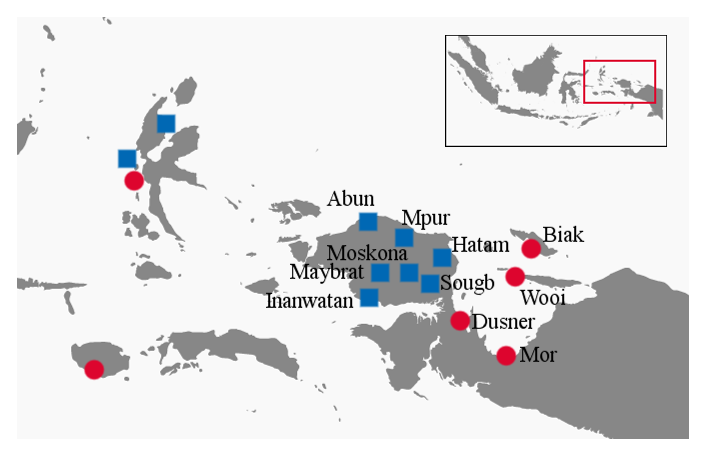
\includegraphics[width=0.7\textwidth]{figures/Map_Papua2.eps}
\caption{Distribution of languages from the Western Papua subarea.}\label{map:Pap}

\end{figure}

I will discuss these languages in three groups. The first group includes the Papuan family-level isolates Abun, Mpur and Maybrat, as well as the \textsc{SBH} language Inanwatan. The languages of this group are all spoken in the north and west of the Bird's Head, Abun and Mpur along the northern coastline, Maybrat further inland on the central plateau, at the foothills of the Tamrau mountain range, and Inanwatan along the southwestern coast. The second group of languages is formed by members of the EBH family and the Hatam-Mansim family. They are all located in the eastern part of the Bird's Head. Third and last comes the group of Austronesian languages, including Biak, Dusner, Mor, and Wooi, which are all located in the Cenderawasih Bay area.

A few typological features apply to (almost) all of these languages (which is why \citealt{reesink2005west} speaks of West Papuan languages in a geographical sense) and can be discussed together. Constituent order in WP  and the Austronesian languages is almost invariably SV/AVO with only Inanwatan showing Papuan AOV order (though direct objects may be placed postverbally, see \citealt[195]{reesink2005west}; also \citealt[52f.]{devries2004}). Almost all languages in the area have argument indexing prefixes on the verb (except Abun; \citealt[5]{dol2007grammar}). Gender is a persistent feature only in the first group (except for Abun), and lacking in the \textsc{EBH} family, in Hatam and in the Austronesian languages \citep[205]{reesink2005west}. A further syntactic hallmark is the placement of the negator which is clause-final, or at least post-predicate \citep[199]{reesink2005west}, tallying well with Himmelmann's  preposed possessor type in Austronesian languages of the area. The high degree of mutual influence between Papuan and Austronesian languages is also witnessed by strikingly similar phonemic shapes of the negators, many of them corresponding to a form \#\textit{va/βa} or \#\textit{te} (see  \citealt[199]{reesink2005west} for discussion).

The three family-isolate languages of the first group, Abun, Mpur, and Maybrat, do not have any established genealogical context and hence are sufficiently different from each other in terms of lexical and grammatical properties.\footnote{Maybrat has in fact been linked to the \textsc{WBH} family (of which no language could be included in the present data set), with traces of cognate structures in pronouns, gender distinction, and verbal prepositions \citep[187]{reesink2005west}.} Inanwatan, on the other hand, as a member of the SBH family, provides some evidence for a distant relationship to the TNG language family. 

Of all WP languages, Abun ``seems to have undergone the highest degree of morphological erosion, even to the extent that verbal affixation is totally absent" \citep[205]{reesink2005west}. Instead of verbal morphology, many grammatical features in Abun are encoded by particles. As there is no argument indexing on the verb nor any case marking, Abun grammatical relations are entirely defined by position, i.e., the subject is always the NP that stands before the predicate \citep[51]{berry1999}. Objects may be fronted if topicalised, and they are also frequently subject of ellipsis. While SVCs do not constitute a distinct topic in Berry and Berry's grammar, they do note in passing that SVCs are not uncommon in Abun, and that there is some variation between speakers as to the placement of pronouns ``to separate verbs" \citep[51]{berry1999}. Examples (\ref{abun1a}) and (\ref{abun1b}) serve to illustrate the basic linguistic structure of Abun clauses, as well as interverbal pronoun placement in SVCs. Note that both constructions involve a \textsc{motion-to-action} sequence, yet the coding differs in both cases according to the presence or absence of a subject pronoun marking the subject of V$_2$. While the first case looks like two juxtaposed clauses and thus arguably corresponds to the Kambera control construction using \textit{pa-}, or to the Selaru linker construction, the second case is the expected unmarked construction that is typical for most of the other languages of EI.

\ea
\langinfo{Abun}{Papuan, isolate}{\citealt[52]{berry1999}}\\
\ea \label{abun1a}
\gll ji mu ji git su-git mo nu \\
\textsc{1}\textsc{sg} go \textsc{1}\textsc{sg} eat \textsc{nmlz}-eat \textsc{loc} house \\
\glft `I went and ate at home.' \\
\ex \label{abun1b}
\gll ye-suk-mise ma nai gwat an mu ket \\ 
\textsc{pers}-\textsc{nmlz}-evil come capture carry \textsc{3}\textsc{sg} go west \\
\glft `The police came and caught him and took him westward.'
\z
\z

Mpur, Maybrat and Inanwatan, on the other hand, function quite differently and index S/A arguments, or S/A and O arguments (Inanwatan) on the verb. Mpur has S/A-indexing prefixes but indexing is only obligatory with human subjects. The 3SG indexer shows a split into masculine and feminine gender. The Mpur pattern is paralleled in Maybrat with the difference that the non-masculine gender is the unmarked gender associated with most nouns (i.e. those without male sexus), and the indexing system appears to be obligatory with all kinds of referents. Bisyllabic verb stems in Maybrat that have a C-initial second syllable do not, however, take overt person prefixes but may be analysed as covertly inflecting for person (see \citealt[52f.]{dol2007grammar} for discussion).

Inanwatan is morphologically more complex and has a linguistic profile that is similar to that of the Marind languages from the south central coast of New Guinea suggesting an old genealogical relationship \citep[16]{devries2004}. De Vries notes that the Marind languages have four characteristic features that are also present in Inanwatan: (i) subject prefix followed by object prefix on the verb in a basic AOV clause; (ii) suppletive verb stems indicating plurality of the subject (and sometimes of the object); (iii) gender systems with agreement phenomena and with front vowels indicating masculine and back vowels indicating feminine gender; and (iv) coordination of fully inflected verbs instead of clause chaining with medial verbs, and no or marginal presence of serial verbs. The following examples illustrate properties (i) and (iii), respectively.

\ea
\langinfo{Inanwatan}{Papuan, SBH}{\citealt[15]{devries2004}}\\
\ea \label{inan1o}
\gll iwáa-go suqére né-i-we-re \\
yesterday-\textsc{circ} sago \textsc{1}\textsc{sg}.\textsc{sbj}-\textsc{2}\textsc{pl}.\textsc{obj}-give-\textsc{pst} \\
\glft `Yesterday I gave you sago.' \\ 
\ex \label{inan2o}
\gll nó-opo-be-re né-ri-be-re né-re-be \\ 
\textsc{1}\textsc{sg}.\textsc{sbj}-take.a.bath-\textsc{prs}-and \textsc{1}\textsc{sg}.\textsc{sbj}-eat-\textsc{prs}-and \textsc{1}\textsc{sg}.\textsc{sbj}-sleep-\textsc{prs} \\
\glft `I took a bath, ate and slept.'
\z
\z

Example (\ref{inan1o}) shows the order of indexers on a ditransitive verb with A and G being indexed while the T argument is only expressed via an NP. Generally, O and G indexing only happens when the object is either the speaker or the addressee, otherwise only S/A is marked on the verb \citep[35]{devries2004}. Inanwatan has another two categories that cause inflection on the verb. First, there are three tenses, past, present and future tense, each marked by a tense suffix. And second, there is the habitual-durative suffix \textit{-rita} (the only aspectual distinction marked that way) replacing the tense suffixes in events that occur habitually, repeatedly or prolonged \citep[38]{devries2004}.

The second example in (\ref{inan2o}) is an instance of Inanwatan clause coordination, a feature that is only marginally (if at all) present in other WP and Austronesian languages of the area. Event sequences of a similar sort may be found in other languages as well, though without overt coordination morphology. There are, however, other multi-verb sequences in Inanwatan that do not receive such coordination marking.

The three languages of the second group, Hatam, Sougb and Moskona, are structurally rather similar. They are all SV/AVO and they have subject prefixes on the verb. Otherwise their verbal morphology is quite simple. Gender as a nominal category is absent from Moskona, but there is a phonological distinction into alienable and inalienable nouns in that members of the former group begin with \textit{m-}. Subject arguments are crossreferenced on the verb and may be omitted if topical \citep[269]{gravelle2010grammar}. Objects follow their verb and can be moved to a pre-posed topic position, as is common throughout the area. Moskona also marks irrealis on the verb by using the prefix \textit{me-/m-}. The irrealis marker comes after the subject prefix and before a potential causative prefix. In negative polarity clauses, the verb always takes \textit{me-} \citep[110]{gravelle2010grammar}. 

Related Sougb also has the Moskona features except for some minor differences: alienable nouns do not show a fossilised \textit{m-} prefix but instead inalienable nouns appear to begin with a vowel \citep[218]{reesink2002grammar}. Verbs in Sougb are also phonologically restricted and begin with a [-\textsc{high}] vowel, either /e/, /o/ or /a/. Sougb verbs may take subject indexing prefixes, the irrealis morpheme \textit{em-}, and the instrument marker \textit{a-}. The combination of these prefixes differs in the three verb classes with regard to vowel realisation in the stem and the prefixes \citep{reesink2002grammar}. The instrument marker is a phenomenon that occurs in a range of languages in the area (also Austronesian ones) and has repercussions for SVC analysis. I repeat two examples of the use of the instrumental prefix from \citet{reesink2002grammar} below:

\ea
\langinfo{Sougb}{Papuan, EBH}{\citealt[205]{reesink2002grammar}}\\
\ea
\gll dan d-eic kepta d-a-(e)hi sogo \\
I \textsc{1}\textsc{sg}-take machete \textsc{1}\textsc{sg}-\textsc{ins}-fell tree \\
\glft `I cut the tree with a machete.' \\ 
\ex \label{sougb1}
\gll dan d-et roti d-a-(e)k kopi \\ 
I \textsc{1}\textsc{sg}-eat bread \textsc{1}\textsc{sg}-\textsc{ins}-drink coffee \\
\glft `I eat bread and drink coffee.'
\z
\z

In the first example, a sequence of two verbs, \textit{eic} `take' and \textit{ehi} `fell' is connected by the use of the instrument prefix reanalysing the O argument of the first verb as the instrument of the second. \textsc{Take}-action sequences are quite common throughout Eastern Indonesia, but the instrument prefix here adds specific morphology to the construction disambiguating the verb string as a coherent unit. This is in contrast to other languages, especially in the Nusa Tenggara subarea, where the verbs are merely juxtaposed without overt argument-flagging. The second example in (\ref{sougb1}) is different as the use of the instrument marker here seems to follow from the fact that ``a previous predicate has introduced an instrument or an accompaniement" \citep[205]{reesink2002grammar}. One might wonder, however, whether the reading `I eat bread and drink it by dipping it into the coffee' would not be preferred here.

Neighbouring Hatam also has an instrument prefix that appears on verbs in verb sequences. In fact, there are two homophonous morphemes \textit{bi-} that seem to express quite related concepts though they clearly occupy different preverbal slots. While instrumental \textit{bi-} appears after the person prefix and before the root, purposive \textit{bi-} comes first in sequence right before the person prefix. The following example illustrates both items in their morphological context.

\ea 
\langinfo{Hatam}{Papuan, Hatam-Mansim}{\citealt[103]{reesink1999grammar}}\\
\gll yoni i-ba micim i-bi-dat dani bigom bi-di-mai \\
they \textsc{3}\textsc{pl}-take spear \textsc{3}\textsc{pl}-\textsc{ins}-pierce I almost \textsc{purp}-\textsc{1}\textsc{sg}-die \\
\glft `They almost killed me with their spear(s).' 
\z

The first instance of \textit{bi-} functions much the way Sougb \textit{a-} does: the O argument of a previous verb is flagged as the instrument of the \textit{bi-}marked verb. Note that the subject of both verbs remains co-referential. The second (purposive) \textit{bi-} does not effect the reanalysis of a previous argument. Rather, what it seems to do is that the whole previous proposition becomes the reason or source for the \textit{bi-}marked action to take place. Another feature of purposive \textit{bi-} is that a change in subjects from V$_1$ to V$_2$ is possible. A further difference between the two markers is that only with instrumental \textit{bi-} which takes up a previous argument the subject prefix marker on the verb may be dropped.

The last group to be discussed here is the Austronesian languages of Western Papua. Dusner and Biak are closely related. Both languages have reduced initial syllables in some roots leading to consonant clusters in the onset that are otherwise rare in Austronesia (for instance Biak \textit{mnu} `village', cf. Wooi \textit{manu} `house'). Wooi and Mor are phonologically simpler and have Austronesian CV(N) syllable structure. All languages make use of person marking on the verb, indexing subjects with prefixes and infixes. Infixes occur in \textsc{2sg} and \textsc{3sg} in Wooi, Dusner and Biak (with consonant-inital verbs, otherwise as prefix) but not in Mor which has only prefixes (zero-marked for \textsc{3sg} on consonant-initial stems). Dusner and Biak have two \textsc{3pl} subject indexers. In Dusner, the split is between human and non-human, while in Biak animate subjects are distinguished from inanimates.

All languages are straightforward SV/AVO and frequently prepose objects. In Wooi, preposed objects need to be crossreferenced by bound resumptive object forms distinguishing between indiviuated object referents and non-individuated (plural) objects. In the following example, the hero Ayraroy (placed in preposed topic position) is killed by his enemies (and is resumptively referred to by the clitic \textit{=i}).

\ea 
\langinfo{Wooi}{Austronesian, SHWNG}{ethnic\_war\_1 081}\\
\glll Ayraroy hemuni \\
A. he-mung=i \\
A. \textsc{3}\textsc{pl}-kill=\textsc{3}\textsc{sg}.\textsc{obj} \\
\glft `They killed Ayraroy.'
\z

Further features of the Austronesian group include clause-final negators, complex determiner and directional systems, instrument prefixes (much like in the EBH languages and in Hatam), as well as prepositions and clause linkers/topic markers developed from verbs. Serialisation seems quite pervasive although there is some variation between Wooi, showing many types of multi-verb strings, and for instance Biak, where verb strings are mostly limited to \textsc{cause-result} sequences. \tabref{table:overviewpapua} lists the crucial syntactic features.

\begin{table}[h]
\begin{tabular}{l r r r}
\lsptoprule
Language & Constituent order & Person marking & Other verbal inflection \tabularnewline
\midrule
Abun & SV,AVO & -- & -- \tabularnewline
Maybrat & SV, AVO & S/A & -- \tabularnewline
Mpur & SV, AVO & S/A & -- \tabularnewline
Inanwatan & SV, AOV & S/A, (O) & tense, aspect \tabularnewline
\midrule
Moskona & SV, AVO & S/A & irrealis \tabularnewline
Sougb & SV, AVO & S/A & irrealis, instrument \tabularnewline
Hatam & SV, AVO & S/A & instrument \tabularnewline
\midrule
Biak & SV, AVO & S/A & instrument \tabularnewline
Dusner & SV, AVO & S/A & instrument \tabularnewline
Wooi & SV, AVO & S/A & instrument \tabularnewline
Mor & SV, AVO & S/A & -- \tabularnewline
\lspbottomrule
\end{tabular}
\caption[Basic verbal features of the Western Papuan languages]{Overview of basic verbal features of the Western Papuan languages in the data set. Constituent order lists only the basic pattern, pragmatically induced alternative patterns are often also possible.}
\label{table:overviewpapua}
\end{table}

\section{Summary}
Summarising the findings from this chapter, we have seen that most of the languages of EI, although genealogically and typologically quite varied, share some basic features, such as argument indexing on the verb and clause-final negation. The Papuan languages appear to fall into at least two areal clusters (leaving aside the North Halmahera languages): the TAP languages are verb-final languages with reduced and irregular undergoer argument indexing on part of their verbs. The West Papuan languages in the Bird's Head area, on the other hand, have converged on a couple of Austronesian features, such as adopting AVO word order and the inclusive/exclusive opposition. The Austronesian languages are more heterogeneous if we take into account the Sulawesi languages, the western outlier Kambera in the Nusa Tenggara group, or the highly isolating languages on Timor, such as \ili{Waima'a}. If we abstract away a little further we may imagine the languages of EI along a west-to-east gradient as tending to lose verbal morphology up to Timor and gaining or preserving verbal morphology yet further to the east in the Northern Moluccas and Western Papua. While person marking appears to be quite constant throughout, TAM marking is prevalent only in the far west and the far east of the area, leaving Nusa Tenggara practically devoid of these verbal categories.

This review has focused on verb morphology for two reasons. First, languages differ as to which categories are marked on the verbs. Second, languages strongly differ in the extent to which verb morphology is used. The challenge here is not only the lack of overt morphology in isolating languages, but also that a set of languages does not have \emph{reliable} verb morphology, in the sense that in annotating verbal inflection in MVCs one is not able to determine whether a given verb is inflected, would potentially be inflected (if it had other lexical or phonological properties), or is in fact uninflected. I will come back to the issue of verb inflectability in \chapref{ch:gram}, where I will have another look at unreliable inflection.

In the next chapter, I will turn to the literature on verb serialisation, and explore in more detail the ways in which these constructions may be conceived of as coherent units. The chapter will then go on to explore the term MVC that is, I will argue, more suitable  for an analysis of the EI dataset than the serialisation concept.
 
\chapter{Setting the scene}\label{ch:theory}
\section{Introduction}
This chapter provides an outline of the theoretical discussion on verb serialisation, picking up the thread from the introductory chapter where I roughly characterised serial verbs as ``underspecified" verb sequences. Reviewing the properties that have been proposed to characterise these strings, I will in this chapter arrive at a revised definition of what to count as such. The last decades have witnessed a sharp increase in studies into verb serialisation, both from a descriptive point of view as well as from theoretical and typological perspectives. The body of literature is so vast that it is beyond the scope of this chapter to fully review and discuss it. I will rather concentrate on some of the most influential contributions and single out the main arguments and features.

This chapter consists of four parts. The first part aims at giving a general overview of the literature. It is here that basic concepts such as monoclausality or argument sharing are introduced. As we proceed, we will see that there are both criteria that are used to delimit serialising constructions from other construction types, as well as criteria that are assumed to account for SVC-internal variation (giving rise to much controversy as to which properties SVCs need to have, and which might be optional or dependent upon areal convergence). 

From the close examination of these different criteria I will then, in the next part, turn to work that has been carried out either within the area of Eastern Indonesia or in adjacent regions on related languages. Specifically, I will review Bril's work on SVCs in Oceanic languages \citep{bril2004complex,bril2007nexus}, Pawley's and Lane's work on SVCs in Kalam (the most well-known serialisation system in a Papuan language; \citealt{Pawley1987, pawley2011event, lane2008kalam}), and finally have a closer look at the areal account of SVCs in East Nusantara by \citet{vanstaden2008serial}. The purpose of this section is to review the different classificatory systems in order to test whether they qualify for the study of multi-verb strings in Eastern Indonesia. While I will, in this book, make use of the more neutral term \textsc{multi-verb construction} (see §\ref{sec:defining} below), the literature survey will help identify important parameters that may be applied cross-linguistically in order to shed light on covert, or at least inconspicuous, differences in the make-up of MVCs across different languages.

In part three, I will introduce the concept of multi-verb construction as an alternative to the serialisation idea. The use of the term multi-verb construction is far less widespread than the SVC concept and its definition is not yet settled. It is, I argue, therefore less laden with presumptions and theoretical restrictions, and better suited to an explorative analysis of multi-verb patterns in EI. 

The final part of this chapter turns to more practical issues and presents an overview of how I evaluated the data sources and which decisions I made concerning the identification of verb sequences. 

\section{Properties of serial verb constructions} \label{section:properties}

In descriptions of serial verbs it is common to start the discussion by giving some justification that the structures in question are indeed serial verb constructions. This is done so typically not by giving a language-specific definition but by listing a set of crosslinguistically valid properties or characteristics. These key characteristics are widely distributed across both descriptive and typological work, and are sometimes assumed to be true without really putting them to the test. 

\subsection{Key characteristics} \label{subsection:keychars}

The ``standard list" of properties includes at least the following items:

\begin{itemize}
\item SVCs are monoclausal
\item SVCs share at least one argument
\item SVCs have the intonational properties of a single clause
\item SVCs are conceptualised as a single event
\end{itemize}

Some points that follow from this are obvious. First and foremost, although verb serialisation is a phenomenon that apparently originates in syntax (a series of verbs crosscutting the traditional clause-linking strategies), most characteristics are drawn from other linguistic areas, for example from prosody or from research into cognition. Only the first characteristic, monoclausality, is directly connected to syntax. The problem with monoclausality is that definitions of ``clause" tend not to be universally applicable so that we end up in a situation where we try to define SVCs by putative universal characteristics that in turn depend upon language-specific features. \citet[298]{haspelmath2016serial} notes that \begin{quote}[s]yntacticians often distinguish between monoclausal and biclausal constructions, and there is a voluminous literature on clause fusion, i.e. synchronic or diachronic derivation of a monoclausal pattern from a biclausal pattern
(restructuring, clause union, coherent infinitives, etc.). However, the criteria for determining clausehood are generally language-specific.\end{quote}

Other parameters are equally problematic. The prosody parameter is sometimes given as ``homogeneous intonation contour" (whatever syntactic constituent might be found underneath), and sometimes the argument also invokes the clause concept (``monoclausal prosody"), assuming that there is a definable prosodic unit that is always and invariably tied to the clause. While the former phrasing presupposes a concept of intonational phrases (IPs) in that particular language, the latter presupposes both a clearly defined IP, and a clause. Similar problems arise with the ``single event" notion.

Maybe it is for this reason that the standard list of defining characteristics has been elaborated by many authors time and again, with the addition of further properties from different linguistic layers. \tabref{tab:keyfeatsvc} presents a list of properties that have been proposed quite frequently, including the standard ones given above. It is certainly not exhaustive but may suffice to delimit the field of the more prominent SVC definitions.

\begin{table}\small
\begin{tabularx}{\textwidth}{QQQ}
\lsptoprule 
Parameter & Test & Literature \\
\midrule \multicolumn{3}{c}{Lexical level}\\\midrule  
  independent verb(s) & construe verbs as simplex predicate & \citet{bril2004complex, Aikhenvald2006, haspelmath2016serial} \\
\midrule \multicolumn{3}{c}{Grammatical level}\\\midrule
  no junctor & insert junctor & \citet{Aikhenvald2006, muysken2006serial, haspelmath2016serial} \\
  monoclausality & apply clause defining operations, relativisation, apply negator & \citet{bril2004complex, Aikhenvald2006, haspelmath2016serial} \\
  no dependency & observe/apply verb morphology & \citet{Durie1997, Aikhenvald2006} \\
  single subject/ external argument & insert different subject referents & \citet{Durie1997, muysken2006serial} \\
  shared argument(s) & insert different argument referents & \citet{Durie1997, bril2004complex}, \citep{Aikhenvald2006} \\
  single predicate/ predication & apply predicate defining operations & \citet{bril2004complex, Aikhenvald2006} \\
  shared operator value & apply different operators & \citet{Durie1997, bril2004complex, Aikhenvald2006, muysken2006serial} \\
\midrule \multicolumn{3}{c}{Prosodic level}\\\midrule
  single pitch contour & check IU defining properties & \citet{Durie1997, bril2004complex, Aikhenvald2006} \\
  no internal pauses & measure speech flow (interruptions) between verbs & \citet{bril2004complex, muysken2006serial} \\
\midrule \multicolumn{3}{c}{Cognitive level}\\\midrule
  single event & apply event defining operations, MEP & \citet{Durie1997, Aikhenvald2006} \\
\lspbottomrule
\end{tabularx}
\caption[Key characteristics of SVCs]{Prominent key characteristics of SVCs and their occurrence in selected publications. Citations in brackets mean that the feature is not regarded as obligatory by the author. Note that the tests are inferred from the literature, and not necessarily proposed or used that way by the specific authors.} \label{tab:keyfeatsvc}
\end{table}

As already indicated, there are basically two types of those. Parameters of the first type can be assessed directly by applying some straightforward operation. For instance, the parameter ``no junctor" may be put to the test simply by trying to add one. Or the independence of a verb may be tested just by putting it into predicate function, i.e., creating a monoverbal predicate. The results of these operations are not always straightforward but at least there is a test available. 

The second type of parameter, on the other hand, relies upon further features that need to be tested beforehand. This is exactly the monoclausality problem from above. This type may be called a dependent parameter because it relies on further information that often need to be gathered from the language in question (i.e., there is no crosslinguistically valid procedure). Examples of this type of parameter all have the test description ``apply X defining operations" in \tabref{tab:keyfeatsvc}. It is these parameters that are most prone to circularity. For example, it is tempting to argue that SVCs only consist of one predicate by resorting to quite unrelated concepts such as clausehood or syntactic dependency, as the following discussion in \citet[4]{Aikhenvald2006} under the header ``[s]erial verb construction as a single predicate" illustrates:
\begin{quote}An SVC functions on a par with monoverbal clauses in discourse... act together as a syntactic whole... [is] often translatable as single predicates into non-serializing languages... cannot take separate markers of syntactic dependency.\end{quote} 

Instead of directly assessing the predicate status Aikhenvald resorts to a range of concomitant feature values such as lack of dependency markers or syntactic unity. The problem of circularity in these arguments is long known. Givón, for instance, has called the single clause/single event arguments ``a problematic straw man" \citep[84]{givon1991serial}. He continues by stating that
\begin{quote}[o]n the structural side, `single clause' is a notion that retains a high potential for circularity. One can
easily define `clause' as a construction with a single verb at its core. On the cognitive side, `single event' is just as susceptible to the very same circular definition, and linguists are notoriously prone to letting grammatical structure define what is a `single event'.\end{quote}

Another circular argument in favour of the monoclausality parameter is also quite common. The evidence that a SVC is monoclausal is often drawn from the fact that it has a ``monoclausal intonation contour". This can of course easily be flipped into the argument that SVCs have a coherent intonation contour just because they consist of a single clause. This way of cycling between the concepts leads to a situation that is crosslinguistically hard, if at all, accessible. As \citet[299]{haspelmath2016serial} points out: 
\begin{quote}[F]rom the current perspective, this is fatal: Comparative concepts must be defined in such a way that the definition is equally applicable to all languages. Applying different diagnostics to pick out the same phenomenon in different languages would make sense only on the view that a notion such as ``clause" is an innate category of universal grammar.\end{quote}

In the following sections, I will have a closer look at the different parameters from \tabref{tab:keyfeatsvc} and discuss the arguments that have been raised in their favour.

\subsubsection{Lexical properties}\label{sec:lexprop}

The most influential parameter on the verb level is the independent verbs parameter suggesting that each verb in a SVC should in principle be able to occur on its own (behaving like a full-fledged independent verb). The first question that arises here is whether verbs are in fact always independent in this sense. Or are there also verbs that are not independent but may only occur in combination with some other item (which then is probably another verb or something quite related)? There are many examples of items that seem verb-like in one regard and yet cannot occur as an independent verb. For instance, auxiliaries or modal verbs show verbal properties in many languages (for instance, they may inflect or occupy the main verb slot in a clause). Another class of verb-like items is the coverb class that pervades the grammar of many Australian languages. Here it is their capacity to provide the argument frame that makes them look quite verbal (although what takes the inflection is a generic verb). Basically because coverbs do not inflect for verbal categories, Schultze-Berndt argues for Jaminjung that coverbs form a distinct lexical category \citep[71]{schultze2000simple}. The ``real" verbs in Jaminjung, on the other hand, are a smallish class of about 30 members and possess quite generic meanings (although simplex predicates with just one of these generic verbs constitute about 40\% of verbal predicates in texts \citealt[118]{schultze2000simple}). The fact that many event concepts in languages such as Jaminjung can only be expressed by combining a coverb and a generic verb (``complex predicates") still suggests that coverbs may qualify as verbs (though certainly not as prototypical ones).

So, the answer to the question: "Are there verbs that are not independent?" is, frankly, yes. There are lexemes that show verb-like behaviour and yet do not fulfill all requirements of verbs in that particular language. Now, on which ground may we qualify or disqualify them as possible hosts in SVCs? Authors that discuss the ``independent verb" parameter seem to assume that multi-verb strings with such verbs do not constitute SVCs because SVCs are viewed as ephemeral combinations of free verbs occurring on the spot without any dependency relations. For instance, \citet[303]{haspelmath2016serial} gives the following definition: \begin{quote}Comparative concept `independent verb’:

for comparative purposes, an independent verb is a form that can express a dynamic event without any special coding in predication function and that can occur in a non-elliptical utterance without another verb.\end{quote}

Two things are crucial in Haspelmath's definition. First, independent verbs express dynamic events. This is remarkable because it is (to my knowledge) the first attempt to disqualify SVCs with stative verbs altogether. \citet[302]{haspelmath2016serial} argues that \begin{quote}the only workable criterion for noun, verb and adjective as comparative concepts is the use of an item in a particular information-packaging function without special coding such as a copula. Thus, verbs are defined as dynamic event expressions that do not have special coding when used in predication function.\end{quote}

The second crucial part in Haspelmath's definition is the ``non-elliptical utterance". Ellipsis is a well-known problem in SVC analysis because elliptical utterances may be mistaken for full-fledged constructions. Consider for illustration the stretch of Wooi narrative in (\ref{wooi_narr}).


\ea \label{wooi_narr}
\langinfo{Wooi}{Austronesian, SHWNG}{traditional\_land\_Kirihio1\_exp 27-29}\\
\ea
\glll Rakuar hembepinda rea \\
Rakuar he-ve-pinda rea \\
Rakuar \textsc{3}\textsc{pl}-\textsc{vblz}-move again \\
\glft `The Rakuar people moved again,' \\ 
\ex \label{wooi-kong}
\glll hengkong hnia na riumpey \\
he-kong hnia na riung-pey \\
\textsc{3}\textsc{pl}-with \textsc{3}\textsc{pl} \textsc{loc} top-\textsc{upward} \\
\glft `they (stayed) with them up there,' \\ 
\ex
\glll hena kuyra na Hopi mariayng vane \\ 
he-na kikuyra na Hopi maria-ayng vane \\
\textsc{3}\textsc{pl}-stay together \textsc{loc} Hopi river-bottom \textsc{det}.\textsc{nprx} \\
\glft `they stayed together at the estuary of Hopi river.'\\ 
\z
\z

If we have a look at the second clause, we encounter a verb that is glossed like a preposition (or a preposition that behaves like a verb). In fact \textit{kong} in Wooi is one of these in-between items that have been called \textit{prepositional verb} in other languages (for instance, by \citet{dol2007grammar} in her grammar of Maybrat). \textit{Kong} in Wooi does not typically take a person indexer when it is used as a postverbal preposition in the sense `do sth. (together) with X' where X denotes a person or a group of people. However, in certain contexts it does inflect and sometimes it occurs on its own, as in example (\ref{wooi-kong}) above. What is interesting here is that our native language specialist added a verb to his Indonesian translation (\textit{mereka (tinggal) dengan mereka di atas}), as if he felt the need to furnish the clause with a ``proper" verb (imitated in the English translation by adding the verb `stay'). In such examples, one could arguably analyse the clause as consisting of an elliptical construction with underlying \textit{hena hengkong} although this would still leave the question why \textit{kong} is marked with the person indexer here. Such data pose serious problems for the question whether (i) a given item is a verb, and (ii) a given item is in fact able to act independently. For the purpose of this study, I excluded all those cases from the sample for which I could not gather evidence that the verbal item in question may also be used as a simplex predicate. Though not every verb has been put to the test, doubtful lexemes such as Wooi \textit{kong} were searched for in other parts of the published data source, and consequently dismissed if no further data points could be found. An exception to this procedure was made with lexemes that had modal or auxiliary verb semantics. These were counted as ``verboid" and assumed to be verbal (but not fully so, as their rather abstract semantics would normally prevent a simple predication). The same goes for verb-like items that by virtue of grammatical restrictions are to co-occur with other verbs (as, for instance, the group of post-verbal modifier verbs in Wooi; see §\ref{sec:identifyingverbs} for a brief discussion).

Modal verbs and their kin are indeed crucial to the discussion of independent verbhood. For instance, by defining \textit{verb} as given above \citet{haspelmath2016serial} tries to exclude examples like English \textit{will go} where the bare auxiliary occurs for instance in elliptical answer formulae such as \textit{Yes, I will}. Other verblike elements that would be excluded on these grounds are, for instance, role-marking verbs in some languages (for instance `accompany/with' or `benefit/for'). 

Another problem with lexical approaches is polysemy between verbs that occur both on their own and in SVCs. \citet{enfield2009review} compared such verb pairs from the descriptive chapters in Dixon and Aikhenvald's edited volume on SVCs and found that the authors handle polysemous verbs quite differently. While some are rather liberal and allow verbs to be semantically related, other authors exclude ``mere relatedness between an item in the two contexts" \citep[448]{enfield2009review}. He concludes that ``[o]pinions will differ as to whether two lexical entries with different but related meanings should be considered `the same verb’."

Summarising the points, the notion \textit{independent verb} seeks to exclude certain classes of elements that exhibit verbal properties. In a certain way, this is problematic since verb serialisation as a concept makes use of the notion \textit{verb}, and verbs are often not explicitly defined as independent predicators. The question ``what is a verb in language x" may then yield a quite different answer from the question ``what is an independent verb in construction Y". As \citet[304]{haspelmath2016serial} concedes, ``[f]rom a language-specific point of view, it may of course still be useful to include these cases [i.e., non-independent verbs, V. U.], e.g. because they may take aspect marking." A further point that remains unclear is how to deal with semantic alternation between verbal items in simplex predicates as opposed to multi-verb predicates. A strict monosemy approach would demand the exclusion of any verbal item that shows contextual deviation in its semantic components.

\subsubsection{Grammatical properties}\label{sec:gramprop}

Under grammatical properties (in a rather loose sense) we can group seven identificational criteria of SVCs: (i) monoclausality, (ii) no dependency, (iii) single subject/external argument, (iv) shared arguments, (v) single predicate/ predication, (vi) shared operator value, and (vii) no junctor.

\textsc{monoclausality}. I have already commented on the difficulties of this argument above. It hinges on how clauses are defined. As \citet[26]{lane2008kalam} remarks, to make such an argument presupposes that ``the clause" exists both as a single notion on which all linguists can agree, and as a linguistic unit that is clear-cut and identifiable across all languages. While typical clauses with one inflected verb are uncontroversial, multi-verbal clauses may show different degrees of compactness of construal. One candidate for clause identification is the classical head as defined by finiteness morphology on the main verb (see also §\ref{sec:headedness} on headedness in the next chapter). As there are many examples of SVCs with two or more inflected verbs in sequence, this approach would need to specify whether all inflected verbs are indeed heads or whether some cases rather involve inflection copying or spread. If verbs are inflected, it is minimally V$_1$ that carries inflection marks in most SVC languages. Cases with V$_{\textsc{fin}}$ inflection seem to be much rarer even in verb-final languages. This result is also found in the EI languages (see §\ref{sec:headedness}).

A second diagnostic for clausehood is the scope behaviour of operators. Such approaches have become especially popular within Role-and-Reference Grammar's (RRG) \textit{layered structure of the clause}. The claim is that different operators target different clausal layers \citep{foley1984functional}. While aspect and directionals are connected to the nucleus, other operators such as tense target the peripheral layer of the clause, i.e., are indicative of the outer boundaries of the clause. \citet{haspelmath2016serial} argues in a similar way for a crosslinguistic clause diagnosis, following \citet{bohnemeyer2007principles}, who observed the behaviour of negators within clauses. Negation as an indicator for monoclausality can be used in at least two different ways. First, one could argue that the scope of the negator has to stay the same. Different authors take different positions in this regard. Examples like the following one from Alamblak (Papua) illustrate that in some languages there are different possible interpretations available. The utterances from (\ref{ala-1}) to (\ref{ala-2}) are all possible replies to the negated serial verb construction in (\ref{alamblak1}), differing in the way the scope of the negator is understood.

\ea 
\langinfo{Alamblak}{Papuan, Sepik}{\citealt[27]{bruce1988}}
\ea \label{alamblak1}
\gll ritm fiñnji tandhi-ak-ni-r-më-t-m \\
insects \textsc{neg} roast-get-go-\textsc{irr}-\textsc{rem}.\textsc{pst}-\textsc{3}\textsc{sg}.\textsc{f}-\textsc{3}\textsc{pl} \\
\glft `She did not roast (and) get the insects (and) go.' \\ 
\ex \label{ala-1}
\gll nɨfrim haynimëtm \\
uncooked she:took:them \\
\glft (negative on `roast') \\ 
\ex
\gll tandhihɨtatañhatë \\
having:roasted:(and):left:(them) she:went \\
\glft (negative on `get') \\ 
\ex
\gll yohre tandhiyakitëhhasiwtm \\
still she:is:roasting:(and):holding:them \\
\glft (negative on `go') \\ 
\ex
\gll nɨfrim hɨtatañhatë yimët \\
uncooked \textsc{sa}:having:left:(them) she:went \\
\glft (negative on `roast' and `get') \\ 
\ex
\gll tandhihatë ruhhasëmët \\
\textsc{sa}:having:roasted:them she:was:remaining \\
\glft (negative on `get' and `go') \\ 
\ex \label{ala-2}
\gll yohre tandhitwëtm \\ 
still she:is:roasting:them \\
\glft (negative on all three roots)\\ 
\z
\z

\citet{Aikhenvald2006} proposed that ``[t]here can only be one negator per SVC. It can either have the whole construction as its scope [...] or part of the construction." Under this view, the Alamblak examples in (\ref{alamblak1}) to (\ref{ala-2}) above would be fine. \citet[293]{Durie1997}, on the other hand, seems to take another stance and defines SVCs as having ``shared tense, aspect, mood and polarity: this is often reflected in a single morphological realization of these operators [...], or in obligatory concord across the verbs [...]." SVC constructions in Paamese, he argues, lose their SVC interpretation as soon as the scope of the negator is over the second verb constituent alone.

A second way to operationalise negator behaviour is by looking at their construal. This is what \citet{haspelmath2016serial} and  \citet{bohnemeyer2007principles} suggest: within one clause, there should only be one negation pattern. That is, if the negator is placed with the second verb, the same construction should not be possible with the negator being placed with the first verb \citep{haspelmath2016serial}. The Alamblak case in (\ref{alamblak1}) to (\ref{ala-2}) would under this view be a well-formed SVC as the negator placement remains constant across all scope variations.

A final interesting piece of evidence for clausehood and clause boundaries comes from the behaviour of reflexive binding. We know from generative research into binding that reflexive pronouns may only be bound within its governing category, i.e., the clause. Reflexive pronouns could thus be a measure of clause boundaries in SVCs. Consider example (\ref{saramaccan1}) from Saramaccan, a creole language from Suriname.

\ea \label{saramaccan1}
\langinfo{Saramaccan}{Creole, English based}{\citealt[299]{muysken2006serial}}\\
\gll di mujee$_i$ da di pikin$_j$ di sopi wasi en-seei$_{*i/j}$ \\
the woman give the child the soap wash \textsc{3}\textsc{sg}-self \\
\glft `The woman gave the child the soap to wash himself (*her) with it.'\\ 
\z

The child is the only argument that can control the reflexive pronoun \textit{enseei}. If the woman \textit{mujee} is the theme of the washing, the independent pronoun \textit{en} would have to be used instead of \textit{enseei}. The construction thus arguably consists of two clauses. Arguments of this sort seem otherwise rare in the literature on serialisation (but see \citealt[514]{baker1989object}) and I have not come across evidence from reflexive binding in EI languages. 

In this book, I excluded the monoclausality criterion for both theoretical and practical reasons (see discussion in §\ref{sec:defining} further below).

\textsc{no dependency}. This argument is somewhat less prominent than others but is repeatedly given. Aikhenvald writes: ``Unlike coordinate or subordinate structures, SVCs cannot, by definition, contain any marker of syntactic dependency" \citep[20]{Aikhenvald2006}. Which markers she has in mind remains, however, unsaid. Vague statements like this are also found in descriptive work. For instance, Baird writes about SVCs in Klon: ``We know that verbs within a serial complex are not subordinate to one another, because of their other structural characteristics" \citep[136]{baird2008motion}. \citet[291]{Durie1997} is more explicit on this, saying that ``one verb is not embedded within or as complement of the other". Though Durie does not refer to morphological formatives but to dependency relations as such, it becomes clear that it is instances of verbal complements that are felt to be different from SVCs. Verbs then should not show non-finite or infinite morphology which would indicate complementation or embedding. Also, according to Durie, complementisers and other hierarchising formatives should be absent from SVCs. 

Dependency in its basic sense means that out of two constituents, one dominates the other so that the latter is dependent upon the former. Dependency is at work in different parts of human grammar but for our purpose, the most relevant dependency type is between verbs and other clausal constituents. Governance is a kind of dependency that holds between a verb and its arguments (see also \citealt{bril2007nexus} on the notion of dependency). If the argument position of a verb is filled by another verb (and its arguments), we get a sentential complement. As structures like \textit{Bill saw that the crocodile was heading towards him} are common in most of the world's languages, most proponents of verb serialisation would argue against lumping complementation together with serialisation. Yet, in many serialising languages, sentential complements look just like other types of SVCs: there is neither dependency marking on the verbs, nor are there overt complementisers. This is why authors like Durie or Haspelmath directly make reference to complements or predicate-argument relations, attempting to keep them out of the group of ``proper" SVCs. Haspelmath writes: ``it is better to exclude them, because they do not belong to the original core of SVC phenomena" \citep[15]{haspelmath2016serial}. Aikhenvald, on the other hand, regards ``serialization of verbs of speech as a subtype of verb serialization as a complementation strategy" \citep[25]{Aikhenvald2006}.   

\textsc{single subject/external argument}. This criterion demands that there be only one subject/ external argument in a SVC. If there is only one overt subject or external argument in the whole construction, then surely we must be dealing with a single clause/single predicate. While it does make good sense with the bulk of SVC types, there is a specific problem with SVCs that obviously encode two different subjects. Consider the Paamese example in (\ref{paamese1}).

\ea \label{paamese1}
\langinfo{Paamese}{Austronesian, Oceanic}{\citealt[55]{crowley2002serial}}\\
\glll inau nuas vuas he:mat \\
inau ni-uasi vuasi hee-mate \\
\textsc{1}\textsc{sg} \textsc{1}\textsc{sg}:\textsc{dist}.\textsc{fut}-hit pig \textsc{3}\textsc{sg}:\textsc{dist}.\textsc{fut}-die \\
\glft `I will hit the pig to death.' \\ 
\z

The construction in (\ref{paamese1}) consists of two verbs, each one marked with a subject indexer. The subject indexed on the `hit' verb, however, does not reappear on the second verb. Instead, the object referent of the hitting is reanalysed as subject of the `die' verb. This has sometimes been addressed as ``pivotal constructions" where one argument is assigned two functions. Quite unlike most other types of SVCs, the switch-function type does allow this kind of conflicting subject index. Such patterns have led some authors to quite surprising interpretations. \citet[292]{Durie1997} remarks on the same construction in Paamese: \begin{quote}Despite the multiple subject prefixes, there can only be one true subject NP in Paamese core serialization. This appears before V$_1$. An attempt to insert a second full subject NP before the second verb changes the meaning of the sentence to a biclausal interpretation.\end{quote}

Of course, he is right in observing that inserting two NPs between the verbs apparently leads to a different construction. Example (\ref{paamese2}) illustrates what happens when the pivotal argument is split up into two NPs each one bearing one function (being co-referential).

\ea \label{paamese2}
\langinfo{Paamese}{Austronesian, Oceanic}{\citealt[56]{crowley2002serial}}\\
\glll inau nuas vuasi kai he:mat \\
inau ni-uasi vuasi kaie hee-mate \\
\textsc{1}\textsc{sg} \textsc{1}\textsc{sg}:\textsc{dist}.\textsc{fut}-hit pig \textsc{3}\textsc{sg} \textsc{3}\textsc{sg}:\textsc{dist}.\textsc{fut}-die \\
\glft `I will hit the pig and it will die.'\\ 
\z

The first thing we notice is that the construction only changes with regard to the number of argument slots.\footnote{One of Crowley's arguments for assuming a biclausal construction here is that one can insert the coordinator \textit{kaa} `and' between \textit{vuas} and \textit{kai} \citep[56]{crowley2002serial}.} It is only in the semantics that we find subtle differences. Example (\ref{paamese1}) appears to describe one coherent process of hitting the pig until death occurs. I assume that the `hit' verb in this sense is understood as happening repeatedly. If the event were to be sliced into small time portions, hitting would probably occur within each portion, and the pig's constitution would progressively suffer with each blow. In (\ref{paamese2}), on the other hand, a biclausal sequential reading is produced, where the hitting seems to be bound in time and only afterwards followed by the death of the pig (which may occur after a delay). 

But what does this mean with regard to the ``single subject" claim? If there is only one ``true subject NP" in (\ref{paamese1}), as Durie claims, what does the second verb index? If prefixes mark subjects in Paamese we would not probably want to say that in a small number of cases (in one particular construction), the same prefix instead denotes the object of the preceding verb, or should be ignored altogether. Alternatively, one would need to claim that there are two kinds of subjects in Paamese: ``minor" subjects, or whatever one might call them, are cross-referenced on the verbs, as usual; higher level ``constructional" subjects, however, do not receive marking but are defined by position of the argument in the construction. Both options are highly unwelcome from both a descriptive and a theoretical perspective, and thus the single subject claim seems rather not helpful. Contemporary authors now rather speak of single semantic roles in SVCs (for instance \citealt{haspelmath2016serial}), and this would intuitively make more sense for constructions like (\ref{paamese1}) where both \textsc{ego} and the pig occupy very different semantic roles (actor versus undergoer, or, more fine-grained, agent versus patient).

\textsc{shared arguments}. In SVCs, there is typically one, or more than one, argument that is ``shared" among the verbs. Argument sharing means that both verbs license arguments of which two happen to be co-functional or at least co-referential. While not including this parameter in his definition of SVCs, \citet{haspelmath2016serial} gives a brief overview of different types of argument-sharing in SVCs. He distinguishes between agent-sharing SVCs and patient-sharing (both with subgroups). Generally, this parameter does not receive much discussion in the literature as it seems to be applicable in a straightforward manner.

If argument-sharing is adopted as a hard definitional boundary, then some putative SVCs have to be dropped. The most controversial cases are probably \textit{ambient serialisation} and cumulative argument SVCs. Ambient serialisation involves a modifier verb with a 3SG subject indexer that takes the other VP as its single argument (much like, for instance, \textit{your coming here, it was quick}). Cumulative argument SVCs are formed by a joint group verb like `accompany' and a further verb. The group verb takes a subject and an object argument, both of which are collapsed into a plural subject indexer on the second verb (\textit{I follow you, we go}-constructions). In both cases, one may argue that no argument is actually \emph{shared} between the verbs. This issue is, like most others, not yet settled, and authors give different verdicts. \citet[12]{Aikhenvald2006} for instance is quite liberal in saying that \begin{quote}[p]rototypical serial verb constructions share at least one argument. Serial verb constructions with no shared arguments are comparatively rare, but not non-existent.\end{quote}
Durie is not quite clear on this point. On the one hand, he demands that ``serial verbs `share' at least one and possibly more arguments" \citep[291]{Durie1997}, while at the same time he happily includes example (\ref{paamese10}) of a cumulative argument SVC from Paamese:

\ea \label{paamese10}
\langinfo{Paamese}{Austronesian, Oceanic}{\citealt[294]{Durie1997}}\\
\glll makurik lovaha \\
ma-kuri-ko lo-va-haa \\
\textsc{1}\textsc{sg}-\textsc{imm}-take-\textsc{2}\textsc{sg} \textsc{1}\textsc{du}.\textsc{in}-\textsc{imm}-go \\
\glft `I take you away with me.' \\ 
\z

According to Durie's analysis, ``the subject of the second verb subsumes both the subject and the object of the preceding verb" \citep[293]{Durie1997}. While this is probably no more ``exotic" from a Western perspective than, say, \textit{you and me, we are friends} would be in English, I would rather call this a sharing of referents than a sharing of arguments as the subject argument of the second clause is grammatically referred to with the 1\textsc{du} marker (and thus is construed independently here).

\textsc{single predicate/predication}. The notion predicate forms part of the traditional core of modern linguistic reasoning and is assumed to have universal applicability on a par with clausehood or intonational phrases. Yet if one looks at contemporary textbooks, one finds that predicate definitions are not as common as would be expected for such a fundamental phenomenon (see also \citealt{baker2010complex}). In Payne's much used guide for field linguists \parencite{payne1997describing}, for instance, verbal predicates are largely absent from discussion. And Kroeger in his \textit{Analyzing Grammar} from 2005 only touches briefly upon the notion in order to introduce the grammatical relations. He writes \citep[53]{kroeger2005analyzing}:
\begin{quote}A statement, then, is a sentence which asserts a proposition, i.e. a claim that a certain state of affairs does or does not exist. Normally statements are made about something or someone; they claim that a certain state of affairs is true of a given individual or set of individuals (where the individual may
be a person, place, thing, etc.). [...] The element of meaning which identifies the property or relationship is called the predicate.\end{quote}
While this seems to be something that undergraduates learn in their first semester, it becomes puzzling as soon as the concept predicate is put to use in a context where there is more than one verb in one (alleged) clause. Predicates (and their predicators) come with a number of arguments and assign grammatical functions to them. As verbs are the most typical predicators in language, each verb may in principle count as one predicate nucleus providing a range of argument slots and assigning a grammatical function to them. There is no reason why this assumption should not hold for verbs in SVCs (which means that SVCs do not automatically defy a multi-predicate analysis).

However, the most common reading of the predicate argument in the serialisation literature suggests that SVCs are multiverbal predicates (that is, monopredicational constructions). \citet{klamer1998grammar} opens her chapter on ``complex verbs" in Kambera with the definition that ``[s]erial or multi-verb constructions in Kambera are combinations of two verbs that jointly constitute a single predicate". This view seems indeed most appealing in languages where several verbs recveive a single set of affixes forming what \citet{foley1984functional} have called \textit{nuclear layer serialisation} (see §\ref{sec:nuclear} below). Consider example (\ref{kambera10}) from Kambera:

\ea \label{kambera10}
\langinfo{Kambera}{Austronesian, CMP}{\citealt[277]{klamer1998grammar}}\\
\gll na-palài nyara-ha$_k$ [da ahu]$_k$ la mbomang \\
\textsc{3}\textsc{sg}.\textsc{nom}-run chase-\textsc{3}\textsc{sg}.\textsc{acc} \textsc{art} dog \textsc{loc} space\_under\_house \\
\glft `He ran after the dogs under the house.' \\ 
\z

We can see that the affix set marking the subject and the object is distributed over both verbs. As the `run' verb is intransitive it seems natural that the object marker attaches to the second (the transitive) verb. Yet we also find combinations of two transitive verbs with the same affix distribution showing that the object suffix in this construction has to attach to the second verb and not to the first. Examples like this one create conflicting evidence for predicatehood. On the one hand, there are clearly two verbs involved that each contribute different arguments. On the other hand, the surface structure behaves like there really is only one (complex) verb predicating the proposition.

Further confusion with this argument is produced where predicate is distinguished from predication. Bril defines complex predicates\footnote{This term \textit{complex predicate} is problematic in itself. Judging from what has been included under the term, complex predicates are a related yet not identical phenomenon to verb serialisation. It covers, among others, coverb constructions in Australian languages, periphrastic causative constructions in Romance languages, auxiliary verb constructions in English (\textit{will go}, precisely the \textit{will} that is elsewhere with great effort excluded from serialisation through the independent verb parameter from above), and many other constructions that involve generic verbs (light verbs, preverbs etc; see \citealt{alsina1997complex}, and \citealt{baker2010complex} for an overview). The gist is that complex predicates typically involve lexical elements that are excluded from ephemeral SVCs with productive combinations of free verbs. What is more, complex predicates are still regarded as one predicate with multiple heads, and not as a series of predicates which together form one predication, as Bril has it. This suggests that the term complex predicate should not be used as a synonym for SVCs so as not to confuse two concepts that are both not well-defined (see also \citealt[49]{butt2010light}).} as ``a sequence of predicates constituting one single predication" \citep[268]{bril2007nexus}. If this is taken literally, it would sharply contrast with the standard assumption that SVCs form a single predicate. Moreover, it would be unclear how predication differs from predicate if both had diverging boundaries. The reason for this rather obscure definition is most probably that it has been phrased this way out of practical considerations. On the same page, Bril states that \begin{quote}[t]he nucleus or predicate is defined as having propositional content; these terms are used in order to avoid the category of ``verb", which is problematic in Polynesian languages.\end{quote} Now, if we replace \textit{predicate} with \textit{verb} we would get back to the standard version: a sequence of verbs constituting one single predication. 

Note that I do not present any kind of test for the predicate parameter at this point. This is simply because I am not aware of any procedure to detect predicate boundaries that would be applicaple in EI languages. For complex predicates in Romance languages, in Urdu and elsewhere, both predicational elements contribute something, and this something leaves traces for instance in the position of object clitics (as in Romance) or in the case marking behaviour of the arguments (as in Urdu; see \citealt[511]{butt2010light}). However, case marking is virtually absent from EI languages, as are rigidly clitised pronouns that would indicate predicate boundaries. The only feasible way to discern predicate boundaries is in my view to look at the syntactic functions and simply count subjects (as I have laid out for the single subject/ external argument parameter above). Constructions with two distinct subjects, as encoded by person marking morphology, would need to be interpreted as depending upon two distinct predicates. This has, however, hardly been discussed in work on serialisation.

\textsc{shared operator value}. If grammatical operators such as tense, aspect, mood, modality, illocutionary force or polarity are marked within a SVC, the claim is that all verbs necessarily share the same operator value. That is, in a given construction there cannot be two conflicting tense values (like past and present marking), or two conflicting markers of illocutionary force. Since this parameter is not always phrased exactly the same way, different subtypes of this definition can be distinguished. First, the scope of a given operator needs to be over the whole SVC. Second, there may only be one operator expressed. Third, there may only be one way of morphosyntactically applying an operator. The last version is what Haspelmath and Bohnemeyer and colleagues assumed for negation in monoclausal constructions (see the monoclausality parameter above). Some authors seem to waver between version one and version three. \citet[8]{Aikhenvald2006}, for instance, defines as follows: 

\begin{quote}Having shared tense, aspect, mood, modality, illocutionary force, and polarity values implies that no independent choice or contrast in any of these categories is possible for the individual components of an SVC. \end{quote}


Further below she allows for redundant operator marking as well as for single marking in SVCs (thus explicitly rejecting the second version, ``only one operator", from above), and finally discusses the Alamblak negation case from (\ref{alamblak1}) above, stating that \begin{quote}[t]he scope of negation can be the whole construction, or any one of its components by itself, or any combination of contiguous components. \citep[8f.]{Aikhenvald2006}\end{quote}

This, however, seems to contradict her opening statement. If the claim is that the operator values of SVC components may not vary, then constructions with a partial negator scope over components constitute precisely that: two different polarity values in one construction. If the negation in (\ref{alamblak1}) is, say, on `roast' we would get something like `Not roasting the insects, she got them (and) went (off)'. Quite clearly, the different verb components here do display varying polarity values.

\textsc{no junctor}. The final grammatical argument runs as follows: If, in a given construction, a junctor (coordinator or sequentialiser) may be inserted between the verbs, then we are not dealing with a SVC but with ordinary coordination or similar clause-linking strategies. This argument comes in two slightly different versions depending on the semantic difference between the constructions. The first version is to treat a V$_x$ V$_y$ construction as a SVC, and the V$_x$ junctor V$_y$ construction (with change in meaning) as a multi-clause construction. The second version is to treat a structure V$_x$ V$_y$ as a case of covert clause-linking if V$_x$ junctor V$_y$ is also possible (without a change in meaning). The first approach thus allows two verbs to form a coordinate structure with a junctor in one case, and a SVC without a junctor in another. The second approach seems to automatically disqualify two verbs as serialised if a junctor may be inserted (even if, in a particular example, no junctor is expressed). The first argument is nicely illustrated by \citet{schapper2009bunaq}. She gives the ``minimal pair" in (\ref{bunaq20}) from Bunaq arguing that there is a clear change in meaning between both constructions:

\ea \label{bunaq20} 
\langinfo{Bunaq}{Papuan, TAP}{\citealt[443]{schapper2009bunaq}}
\ea \label{bunaq2a}
\gll Baqi n-ege il a. \\
\textsc{nprx}.\textsc{an} \textsc{1}\textsc{ex}-give water drink \\
\glft `He gave me water to drink.’ \\ 
\ex
\gll Baqi n-ege il soq, a. \\ 
\textsc{nprx}.\textsc{an} \textsc{1}\textsc{ex}-give water \textsc{seq} drink \\
\glft `He gave me water, then (I) drank (it).’\\ 
\z
\z

The difference in meaning is most often rendered into English with a purposive translation for SVCs (do x to do y, cp. (\ref{bunaq2a}) above), and a sequential translation involving an overt sequentialiser for non-SVCs (do x then do y). (\ref{abui20}) has another pair from Abui:

\ea \label{abui20} 
\langinfo{Abui}{Papuan, TAP}{\citealt[349]{kratochvil2007grammar}}
\ea
\gll moku me yai paneng \\
kid come song make \\
\glft `The child came to sing.’ \\ 
\ex
\gll moku me ya yai paneng \\ 
child come \textsc{seq} song make \\
\glft `The child arrives and sings.’\\ 
\z
\z

The problem with such examples is that often the same SVCs are, in other contexts, happily translated with coordinate structures just like overt coordination (do x and do y), sometimes with a note that the coordinator in the translation should not be taken literally. From all \textsc{motion-to-action} MVCs in my sample, roughly one half is translated into English purposive constructions and the other one is given with coordinated verbs. This is, however, not consistent across the different languages, and I am not aware that any author has provided more information on the exact semantics of that construction. Therefore my point here is that we are still quite far off from really understanding the semantic difference we are trying to elicit by adding junctors to putative SVCs. 

\subsubsection{Prosodic properties} \label{sec:prosodic}

The prosody arguments in the literature are conveniently given without much demonstration. Some authors give examples with idealized f$_0$ contours, other authors do not. Seldom is there any discussion of actual prosodic data from natural speech. In principle two different arguments can be distinguished though they often get conflated. 
\textsc{no internal pause}, and \textsc{single intonation contour}. The first argument is concerned with (the lack of) breaks in the prosodic output. The verbs in a SVC are argued to occur within a continuous speech flow without displaying signs of hesitation or processing pauses. The idea behind this is that during fluent production, the SVC is conceptualised as a single unit, and the speaker does not have to pause at certain points in order to search for lexical items. In the second argument, the syntactic boundaries of the SVC are considered to be coincident with the prosodic boundaries, that is, the prosodic behaviour is congruent with the putative underlying cognitive and syntactic unit. As any field linguist can tell, this is a gross oversimplification of the matter, and in many cases not true.

Sometimes the first argument makes reference to the second, or even to a ``monoclausal intonation contour", which is, however, a different thing and only indirectly related to pauses (as not every intonation phrase needs to be related to a rhythmic boundary cue such as a planning pause). For some authors, these two arguments still seem to be the same. For instance, in her description of motion SVCs in Keo, \citet[56]{baird2008motion} puts the prosodic argument as follows: ``The construction falls under one intonation contour. That is, there are no pauses between the verbs in a serial construction." Statements like these, however, conflate two quite different things. A coherent intonation contour is not necessarily coherent by the fact that it is delimited by pauses. In many languages, sequences of IPs may be articulated in fast succession without audible pauses. \citet{himmelmann2018} have dubbed such missing boundary pauses \textit{latching} as the IPs are directly latched together. This phenomenon has for instance been demonstrated for the EI languages Papuan Malay, Waima'a and Wooi. The sequence of two IPs in (\ref{Wooi_Oni}) is part of a pear story narration in Wooi. There is a clear IP boundary right in the middle after \textit{intene vat} but this is only indicated by a small pitch jump of about 30Hz between \textit{vat} and following \textit{ve} (cf. \ref{fig:Wooi_Oni}). A lack of pauses between IPs occurs frequently when the speaker is in a ``narrative flow", not just in Wooi but in all other languages of the area I am familiar with.

\begin{sidewaysfigure}
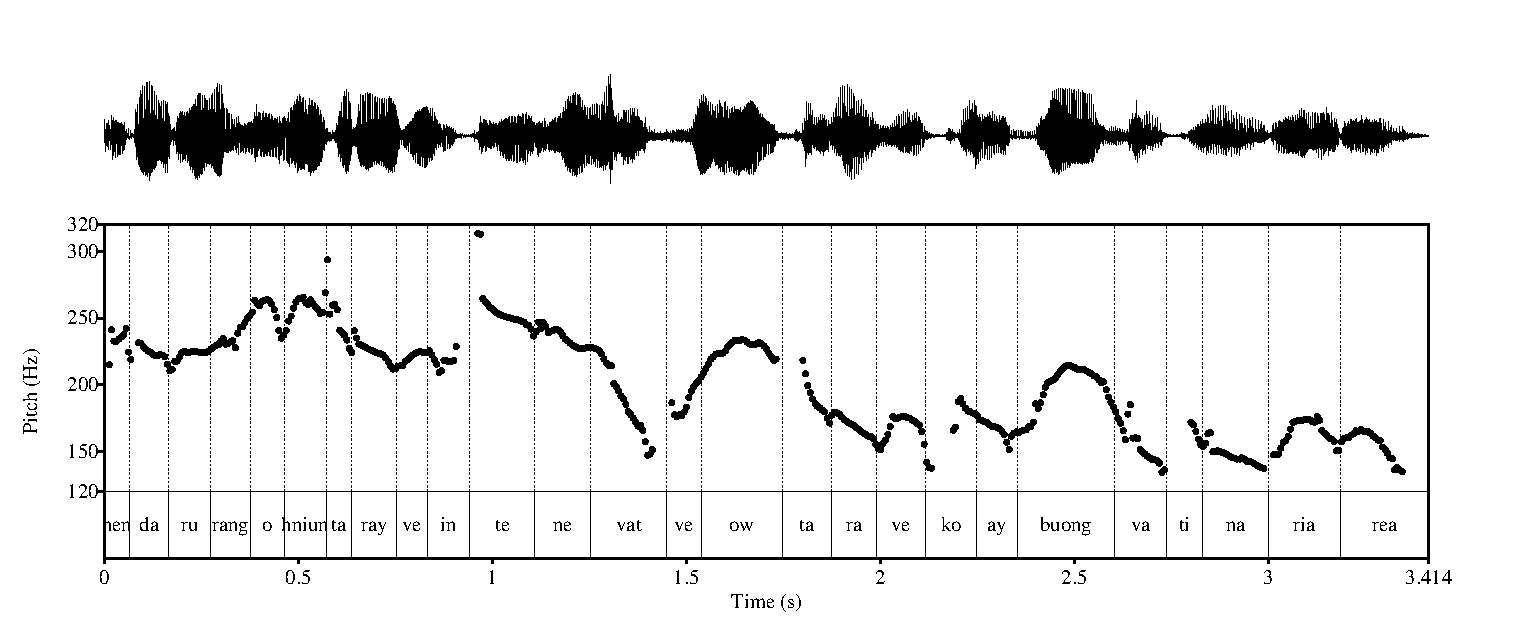
\includegraphics[width=\textwidth]{figures/pearOniLATCH.eps} 
\caption{F$_0$ contour of example (\ref{Wooi_Oni})}\label{fig:Wooi_Oni}
\end{sidewaysfigure}

\ea \label{Wooi_Oni} 
\langinfo{Wooi}{Austronesian, SHWNG}{WBW\_pear\_Oni}
\ea
\glll henda rurang o: hniuntaray ve intene vat \\
he-ra rurang o: hniuntaray ve intene vati \\
3\textsc{pl}-go parallel \textsc{fill} person \textsc{rel} earlier \textsc{det}:\textsc{sg} \\
\glft `They walked alongside the man from earlier,' \\ 
\ex
\glll ve owta ra ve ko aybuong vat naria rea \\ 
ve owta ra ve ko aybuong vati naria rea \\
\textsc{rel} climb go \textsc{rel} take fruit \textsc{det}:\textsc{sg} again  \\
\glft `the one who climbed up who took the fruit again.'\\ 
\z
\z

Furthermore, the opposite assumption is not true either. There are in fact coherent intonation contours that exhibit internal pauses. Pauses are therefore not automatically a cue for a phrase boundary. When a speaker hesitates at a certain point, the f$_0$ value at cut-off may be remembered and resumed at exactly the same level after the pause. This is to be understood as a continuation and not as a phrase boundary. Consider example (\ref{Wooi_John}) from another Wooi pear story narration. In contrast to the case in (\ref{Wooi_Oni}), the speaker resumes the intonation contour at almost exactly the same pitch level as it was on \textit{na} right before the hesitation pause (if one were to cut out the pause, both ends of f$_0$ would fit together quite well; cf. \ref{fig:Wooi_John}).

\begin{figure}
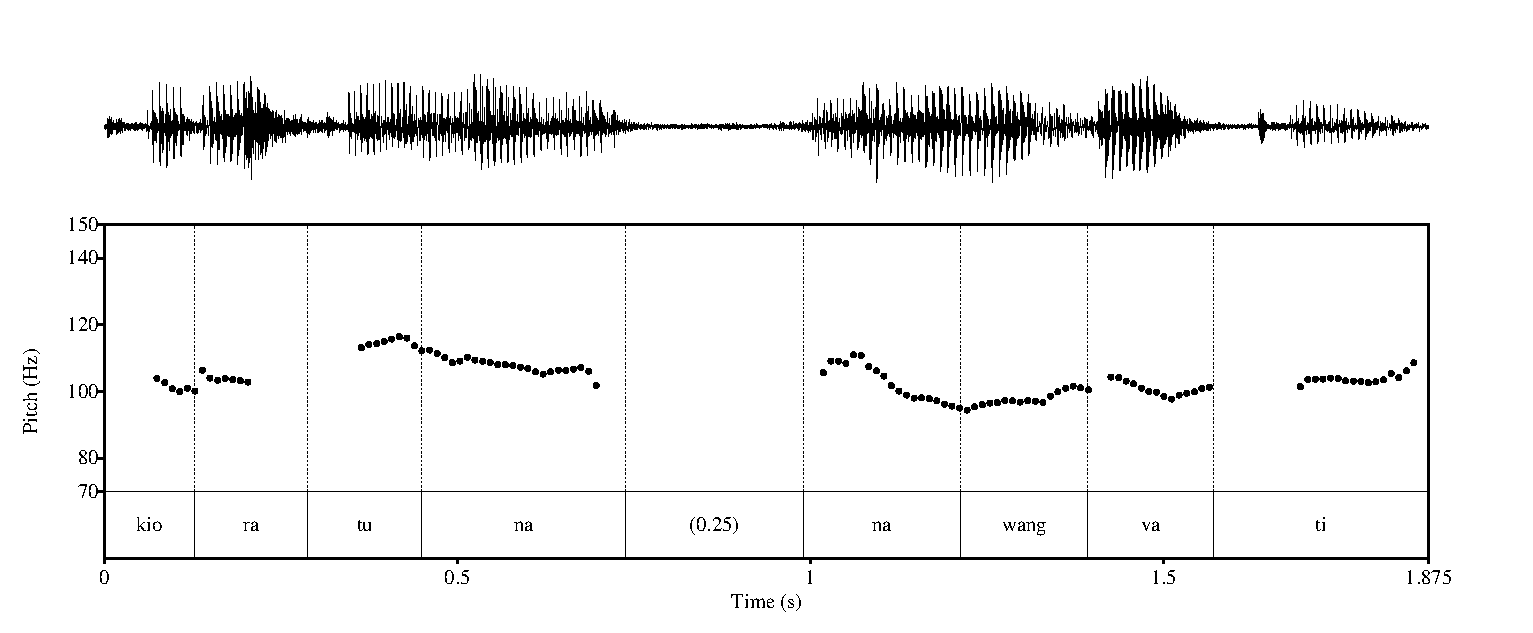
\includegraphics[width=\textwidth]{figures/pearJohnHESIT.eps} 
\caption{F$_0$ contour of example (\ref{Wooi_John})}\label{fig:Wooi_John}
\end{figure}

\ea \label{Wooi_John}
\langinfo{Wooi}{Austronesian, SHWNG}{WBW\_pear\_John}\\
\glll kio ra tu na (0.25) nawang vati \\
$<$i$>$ko ra tura na (0.25) nawang vati \\
$<$3\textsc{sg}$>$take go stand \textsc{loc} (0.25) basket \textsc{det}:\textsc{sg} \\
\glft `He took (them there and) left (them) in the basket.' \\ 
\z

So, to conclude at this point, the observation behind these arguments is that prosody seems to indirectly cue the existence of SVCs. There is certainly some sense in this argument if we look at ``minimal pairs" such as (\ref{bunaq2}) given by \citet{schapper2009bunaq} from Bunaq:

\ea \label{bunaq2} 
\langinfo{Bunaq}{Papuan, TAP}{\citealt[442]{schapper2009bunaq}}\\
\gll Markus bola wa rebel \\
Markus ball discard descend \\
\glft `Markus threw the ball away downwards.’ or `Markus threw the ball away, (and he went) downwards.’\\ 
\z

Depending upon prosodic output, the example in (\ref{bunaq2}) may have two quite different readings. If uttered under a ``single" intonation contour with a high boundary tone aligned to the first syllable of \textit{rebel}, the construction is interpreted such that it is the ball that descends. However, if there is a prosodic break between \textit{wa} and \textit{rebel}, and a final high tone is aligned to \textit{wa}, the interpretation is that it is Markus that descends after discarding the ball (thus making it two distinct event frames) \citep[442]{schapper2009bunaq}.

There is, however, a shortcoming with this argument. If a coherent f$_0$ always cues an SVC, and an incoherent contour automatically precludes an SVC interpretation, then it would follow that the prosody-syntax mapping is exactly one to one. This would be a challenge for already established syntactic units such as the monoverbal clause. We know that clauses do not always neatly align with prosodic phrases (neither with \textsc{IP}s nor with intermediate phrases; see on this point e.g. \citealt{chafe1994discourse}, \citealt{himmelmann2006challenges}, \citealt{ladd2008intonational}, also \citealt{engelhardt2010}), and, indeed, I do not think that it is an exaggeration to claim that we do not know of \emph{any} syntactic unit with a constant prosodic output. Even if, ideally, speakers attempted to match syntactic clauses with coherent prosodic units, natural speech would always remain imperfect. As every field linguist is well aware, ``the physical manifestations of psychologically relevant units are always going to be messy and inconsistent" \citep[58]{chafe1994discourse}. Therefore we would expect that the prosodic chunking of SVCs is subject to variation just as it is found with other syntactic units. Seen this way, the explanatory power of the prosodic argument seems to be less strong and less reliable as is suggested by the standard reading in the literature. While there might be a partial correspondence between prosodic phrases and SVCs no exclusive argument can be based on prosodic behaviour. Yet, as this criterion is almost always used in order to determine SVCs, it has been adopted in the present study for practical considerations (see section §\ref{sec:defining} for discussion).

\subsubsection{Cognitive properties} \label{sec:cognitive}

The last parameter pertains to the cognitive background of SVC construals. It is claimed that SVCs express on the grammatical level what is on the cognitive level perceived as a single event. This claim is probably also the most controversial one and has been dismissed or called into question by many authors. What does \textit{event} mean? One word of caution is in order here. There are at least two meanings of \textit{event} in linguistics. What the typologists and descriptive linguists working on serialisation mean by \textit{event} is quite different from what semanticists have in mind. The latter use is probably older, dating back in its modern sense at least to Vendler's verb class analysis \citep{vendler1957verbs}. Here, event refers to a class of verbs (to the exclusion of stative and activity verbs) that can be deduced by testing their lexical aspect. Events in this sense are roughly equivalent to ``dynamic verbs", or to ``dynamic events" in Haspelmath's \citep{haspelmath2016serial} sense. \textit{Events} in the serialisation debate are not clearly defined but, very roughly, pertain to chunks of space and time in which something is happening (for instance, a basket of pears is stolen, or a pig is dying) and this something is perceived as having a starting point and an end point. The trouble starts when it comes to the question of how these delimiters can be detected. Aikhenvald's definition patently demonstrates the challenge:

\begin{quote}[S]emantically, serial verb constructions may encode one event, or several subevents closely linked together, or even several subevents in sequence which may be conceptualised as connected to each other. In the latter case, it may appear hard to draw a tight semantic distinction between a monoclausal serial verb construction and a sequence of clauses. \citep[12]{Aikhenvald2006}\end{quote} 

There are several problems with this definition, both terminological and theoretical. First, we encounter two different concepts: events and subevents. What is the relationship between events and subevents? Does every event consist of subevents, and if so, of how many?\footnote{Aikhenvald speaks of ``indissoluble" events which implies that there might also be events without a compositional structure \citep[12]{Aikhenvald2006}.} What sounds like a part-whole relation is actually not defined by theory (see also \citealt[499]{bohnemeyer2007principles} on this point). If, by analogy, we compare \textit{events} with syntactic units like \textit{verb phrases}, one could wonder whether events are also projected by subcomponents, that is, whether events are hierarchical in ways similar to constituent structure in syntax or to phonological structure. Yet there has been no real attempt in the serialisation debate to address such questions. 

A further terminological problem with Aikhenvald's definition arises with the phrases ``subevents closely linked together" and ``subevents [...] conceptualised as connected to each other". What exactly is the difference between subevents being linked together and subevents being (conceptually) connected? As long as such notions cannot be made operational and useful to typological approaches, nothing is gained by including such claims into definitions of a phenomenon that is in and of itself only vaguely characterisable. Obviously, what authors have in mind when they speak of subevents is plainly the lexical condensation points of human event perception and segmentation, that is, verbs. My impression is that ``different subevents connected together" is often interchangeable with ``different verbs connected together". \citet[15]{haspelmath2016serial} makes a similar point in remarking that

\begin{quote}[a]s far as I can tell, whenever a clear contrast between a single event and multiple events has been noted, it makes the same distinction as the grammatical criteria, in particular
monoclausality and biclausality.\end{quote}

He then concludes that the event parameter is not a necessary criterion for SVC determination. While that is certainly right at this point, I want to briefly introduce two approaches that have tackled the event concept from different angles. The question that Bohnemeyer and colleagues \citep{bohnemeyer2007principles, bohnemeyer2011} posed was: how should linguistic event segmentation be measured? Instead of matching event boundaries with syntactic or prosodic boundaries, they took the temporal frame of event expressions as their starting point and developed the \textit{macro-event property} (MEP). A MEP is defined as follows:

\begin{quote}A construction has the MEP if temporal operations such as time adverbials, temporal clauses, and tenses necessarily have scope over all subevents encoded by the construction. \citep[497]{bohnemeyer2007principles}\end{quote}

Whether or not a given construction has the MEP can be tested by applying a temporal operator. Thus, in the following example from \citet[503f.]{bohnemeyer2007principles}, (\ref{bohne1}) has the MEP, but (\ref{bohne2}) does not.

\ea
\ea
\label{bohne1} Floyd went from Rochester via Batavia to Buffalo.
\ex *Floyd went from Rochester at seven via Batavia at seven forty-five to Buffalo at eight thirty.
\ex \label{bohne2} Floyd left Rochester, passed through Batavia, and arrived in Buffalo.
\ex Floyd left Rochester at seven, passed through Batavia at seven fortyfive, and arrived in Buffalo at eight thirty.
\z
\z

While temporal modification of each constituent is fine with the multi-clause example in (\ref{bohne2}), it does not work with the monoclausal event conceptualisation. Modifying each PP with a temporal operator sounds odd to English speakers, and signals, according to Bohnemeyer and colleagues, that the whole construction has the MEP.

Another approach to identifying event boundaries comes from neuropsychological research, methodologically established by \textcite{newtson1976perceptual}.\footnote{Many thanks to Rebecca Defina for pointing that out to me.} \textcite{zacks2007event} and \textcite{zacks2010we} report findings from perceptual psychology and cognitive neuroscience showing that humans make use of automatic and incremental event segmentation in order to help predict what comes next and to cope with narrow information uptake \citep{zacks2010we}. In one experiment, participants watched films of everyday activites and had to press a button whenever they felt there was an event boundary. They did this twice. One time they were asked to segment the smallest meaningful event units, and another time they were asked to segment the largest units that were meaningful to them. The results were so consistent that it was argued that they show naturally occurring perceptual processing \citep[80]{zacks2007event}. In other experiments, participants viewed the video clips passively the first time before they were asked to do the segmentation. The segmentation data were then compared to brain activity data. Such data seem to suggest that event segmentation is something that we humans do all the while when we actively engage with the world. However, as \citet[81]{zacks2007event} noted, 

\begin{quote}there is evidence
that observers can adapt their performance of the buttonpressing
segmentation task based on situational needs. For
example, observers adjust the temporal grain of their segmentation
based on explicit instructions, the sort of information they
are trying to learn from a stimulus, and how much they know
about the activity they are watching.\end{quote}

We have seen in the introductory chapter that the ``all-new approach" sets out from the assumption that SVCs are essentially different from clause linkage types, and might therefore reflect underlying differences in event perception and construal. A recent study by \citet{defina2012conceptual} looked into memory effects associated with the use of different grammatical constructions, raising the question whether the use of SVCs might bear on the ability of speakers to recognise and retrieve events. Speakers from English and Avatime (a Niger-Congo language with extensive use of serialisation) were asked to memorise short video clips of putting and taking events. Defina and Majid showed that false recognition of putting and taking events was more likely in Avatime when speakers produced SVCs in a \textit{post hoc} event description, whereas English speakers showed no difference in event recognition with regard to different grammatical constructions. Such findings may suggest that speakers of serialising languages can group event elements together, and store them as event units.

Summing up this section, although evidence from cognitive research amounts to the understanding that event segmentation is a naturally occurring human task, it is still controversial how this is actually reflected in linguistic chunking. Bohnemeyer and colleagues propose that event chunks are basically defined by their inherent temporal properties. Thus, temporal modification seems to be the most reliable test so far in order to detect the boundaries of ``deeper" mental units that are different from better known linguistic units such as the clause.

\subsection{Coherence or composition} \label{sec:coherence}

In the previous sections, I discussed cues to SVC detection that are regarded as standard arguments throughout most of the contemporary literature. In the following sections, I will introduce some further concepts that are not directly used as cues but form a more general backdrop of reasoning. The first idea to consider here is the concept of coherence. What makes a string of elements a coherent construction? All arguments introduced above as part of the standard list of arguments are actually based on a notion of coherence. The verbs form a coherent syntagma (the clause) on the basis of a coherent prosodic pattern, a coherent cognitive conceptualisation, as well as a coherent set of referents that is turned into shared grammatical arguments. All this reveals an important presupposition that is not always made explicit: that SVCs indeed constitute a unit (or construction) and do not consist of juxtaposed clauses (or VPs). This coherent unit has been addressed by features from different linguistic levels assuming that the boundaries of the phenomenon show through the different layers of the language system (for instance, by prosodic chunking). This direction is in line with the ``all-new approach" that I outlined right at the beginning of the introductory chapter. The premise is that this unit is different from the traditionally recognised linguistic units (monoverbal clause, biclausal sentence). 

The presupposition of underlying coherence is, however, not prevalent in all approaches. Mostly in older contributions, we find proponents of the ``nothing-new approach" that assume that there is, though covert, an asymmetry in the verbs' ranking, and that two VPs are linked together in ways similar to complementation or subordination strategies in other languages. A good example for this line of reasoning is Seuren's proposal of serialisation as an instance of pseudocomplementation. He defines pseudocomplementation as follows \citep[196]{seuren1991definition}: 

\begin{quote} A pseudocomplement is a suppositious sentential complement, foisted on a verb whose meaning requires no such complementation, and expressing concomitant circumstance, purpose, or result. Pseudocomplements are opposed to proper complements, which are semantically required by the governing verb.
\end{quote}

Thus, in essence, what Seuren has in mind is an adjunct VP\footnote{as opposed to cases of lexically governed pseudocomplementation such as in \textit{John went fishing} versus \textit{*John walked fishing} where the verb \textit{go} allows for a pseudocomplement whereas other English motion verbs do not (see \citealt[197]{seuren1991definition}).} tied to a matrix VP by specific grammatical rules. First, ``a controlled deletion (or non-expression) of the subject of the pseudocomplement", and second, (optional) ``tense and/or agreement copying from the higher verb" in order to explain double-marked verb strings \citep[197]{seuren1991definition}.

The pseudocomplement approach and similar takes on verb chains aim at saving the generativist model of a single clausal head. \citet{baker1989object} also argued for an analysis that would leave the basic assumptions of the by-then version of government-and-binding intact. Baker proposed a system of double $\theta$-marking where both V$_1$ and V$_2$ $\theta$-mark the shared object argument of a given SVC in any SVO language. One of the outcomes of his proposal was an asymmetry in the status of V$_1$ and V$_2$, with the former verb being a structural sister to the object argument, and the latter being its structural daughter. \citet{Durie1997} has argued convincingly against such an analysis, pointing out that Baker's approach is not consistent with the data.

Whatever the theoretical backdrop of composite approaches is, they do raise the question about what it is that makes us so sure that underspecified verb sequences really form a coherent unit, or even more specific, a construction, as the standard term \textit{serial verb construction} has it. Although it appears from the contemporary literature on serialisation that the coherence side has won the day, the issue of composition will resurface in later chapters of this book, and we will ultimately see in \chapref{ch:discussion} that both coherence and composition do seem to play a major role in the formation of MVCs in EI.

\subsection{Construction and productivity}\label{sec:construction}

In what sense, then, are SVCs constructions? In contemporary linguistic theories, there are at least two definitions of \textit{construction}, a loose one and a strict one. While the loose one is used more or less as a desriptive cover term for a grammatical unit that consists of several items (lexemes and formatives), the strict one has a more narrow definition. For instance, \citet[4]{goldberg1995constructions} defines a construction as follows: 

\begin{quote}Constructions are taken to be the basic units of language. Phrasal patterns are considered constructions if something about their form or meaning is not strictly predictable from the properties of their component parts or from other constructions. That is, a construction is posited in the grammar if it can be shown that its meaning and/or its form is not compositionally derived from other constructions existing in the language.\end{quote}

If SVCs are viewed this way, we would assume that the meaning of the construct contains more than just the sum of the verb meanings. In other words, understanding \textit{construction} in its strict sense entails the postulation of non-com\-posi\-tion\-al meaning in SVCs. Reconsider the Bunaq example in (\ref{bunaq2}) from §\ref{sec:prosodic}. There are two verbs in sequence, indicating a downward movement of the ball away from the actor. To make it non-compositional in Goldberg's sense, the construction would need to convey a meaning that cannot be inferred from the meaning of the two verbs expressed in isolation. Indeed, as we have seen, prosody may coerce two quite different readings. The utterance could be interpreted as a complex motion event where it is the ball that descends. This entails a change in the alignment of syntactic function and semantic role (the theme-object of V$_1$ becomes the actor/theme-subject of V$_2$). Otherwise, if prosodically phrased in a different manner, one might read the sequence as consisting of two events, both performed by one and the same actor (throwing the ball, and then going). If the claim is that reading 1 is preferred under a coherent intonation pattern, then one could argue that the construction as such selects the change in alignment, and neither of the verbs would suggest so when viewed in isolation. Indeed, there is good reason to adopt such a constructionist perspective on multi-verb strings, and I will assume in later chapters (in particular in \chapref{ch:constructions}) that there are underlying constructional schemes at work.

Yet, as far as I can see, the whole discussion of SVCs actually makes very little reference to the concept \textit{construction} (other than carrying it in its name), and does little to explain the consequences that the term might entail in a strict sense. An exception is \citet{haspelmath2016serial} who explicitly refers to constructions. He puts it as follows:

\begin{quote}To fall under my definition, a serial verb construction must be a productive schematic
CONSTRUCTION such that the meaning of a concrete construct can be determined on the basis of the meanings of its parts and the construction meaning. This means that non-compositional combinations of verbs do not fall under the definition. (\citealt[6]{haspelmath2016serial}; emphasis by the author) \end{quote}

Strictly speaking, ``concrete constructs" that consist not only of lexical meaning components but also of ``constructional meaning" are to be considered non-compositional according to standard definitions in literature on constructions (see for instance \citealt{goldberg1995constructions, goldberg2006constructions, croft2001radical}). Understood from a constructionist point of view, Haspelmath's definition that ``non-compositional combinations of verbs" are not considered would probably leave \emph{no} SVC at all in his basket. This is in all likelihood not what he had in mind. Non-compositional in Haspelmath's sense rather seems to be equivalent to non-productive. This is, however, not exactly the same. There are both productive and unproductive SVCs in many languages but both types are non-compositional rather than compositional. Take for instance the position-action construction in (\ref{wooi10}) from Wooi (on position-action, see discussion in §\ref{sec:position-action}).

\ea \label{wooi10}
\langinfo{Wooi}{Austronesian, SHWNG}{frogstory\_Kosmus}\\
\glll hninyong katung mey teti tatuva wona pi \\
hninyong katung $<$i$>$mahoy $<$i$>$tati tatuva wona pi \\
 child little $<$\textsc{3}\textsc{sg}$>$sit $<$\textsc{3}\textsc{sg}$>$peek along dog \textsc{det}.\textsc{sg} \\
\glft `the child sat staring at the dog.'\\ 
\z

We find two meaning components at work: first, there is the meaning of the two verbs \textit{mahoy} `sit' and \textit{tati} `peek' (ignoring the postverb \textit{tatuva} for the moment). Second, there is a meaning component that directly resides in the construction: neither the semantics of the `sit' verb nor of the `peek' verb tell us that both events go on simultaneously. For Wooi speakers the reading of this construction is always that of assuming a position and doing something at the same time. Such non-compositional meaning components are most probably inherent in most, if not all, SVCs. So, as a consequence I would rather assume (\textit{contra} Haspelmath) that canoncial SVCs are inherently non-compositional.

Productivity is a further parameter that is often invoked. As Haspelmath put it, ``good" SVCs are considered productive and schematic (which makes them different from lexicalised constructions such as Zwicky's dismissive \textit{go jump in the lake}; \citealt[9]{zwicky1990we}). Productivity seems to presuppose a construction with slots into which verbs from certain semantically or functionally defined classes may enter. A construction then is productive if it would minimally allow new verbs into one of its slots. If one wanted to get rid of someone, \textit{go leap in the lake} or \textit{go jump in the bathtub} would most probably not have the same effect as \textit{go jump in the lake} precisely because there is no slot available that would allow new items. While the thought of productive SVCs seems appealing at first, we do know of many examples from the literature where authors discuss limits to productive patterns. An oft-repeated pair of examples, one licit and one illicit, is from \textcite{sebba1987syntax}:

\ea 
\langinfo{Sranan}{Creole, Atlantic}{\citealt[60]{sebba1987syntax}}
\ea
\gll a teki a fisi seri \\
(s)he take the fish sell \\
\glft `(S)he sold the fish.' \\ 
\ex
\gll *a teki a fisi bay \\ 
(s)he take the fish buy \\
\glft intended: `(S)he bought the fish.'\\ 
\z
\z

While taking the fish to sell it is fine, taking the fish to buy it is rejected by speakers of Sranan. Durie has referred to such limitations as ``the unacceptability of non-events" \citep[327]{Durie1997}, proposing that the latter sequence is not a proper ``stereo-typical schema" for event-types in that particular language. I do not want to call this explanation into question. Yet it seems plain that ``productive" SVCs are not quite that productive, and that there is a number of language-internal or crosslinguistic restrictions at work. Even constructions that seem to be among the most productive ones, such as the highly frequent motion-to-action construction in EI languages with a motion verb followed by an action verb, are somehow restricted. Rarely have I seen any example of a motion-to-action construction in the EI data that would not feature an action verb in V$_2$ where the action is brought about willingly and the actor is in full control of the situation. There is nothing like `he went fell into the lake' or `he went noticed the child' which suggests that the construction as such has a meaning component \textsc{go somewhere + do something volitionally}. This precludes a large class of verbs that come with a non-volitional or non-control reading.

Productivity is thus a problematic concept. First, it does have clear limitations as a result of which fully productive SVCs probably do not exist (see also \citealt[40]{sebba1987syntax}). And second, no author has to my knowledge tried to make productivity operational by using some measure of quantification. Is a construction productive if it allows, say, twenty different verbs into one of its slots? Or is a construction productive if it allows all verbs of one semantic class (or field)? And if so, how can we delimit the semantic class? As long as these questions are not answered it does not make much sense to speak of productive SVCs unless we only want to emphasize that they are different from fixed lexicalised chunks. Productivity (as so many other linguistic parameters) is thus rather a matter of degree than a matter of either/or\footnote{Enfield made a related point regarding symmetrical and asymmetrical constructions, claiming that the choice between ``restricted" and ``unrestricted" verb slots (or rather verb classes, as some authors misleadingly claim) is rather a matter of personal intuition than of objective criteria. He writes: ``Though the distinction open versus closed is ostensibly discrete, there is much range in what is taken by different authors to fall into one or the other type, illustrated, for example, by the possibility of positing `closed classes’ with as many as 100 items (in Dumo; Ingram’s chapter, 202), or even 600 items (in Ewe; Ameka’s chapter, 125)" \citep[449]{enfield2009review}.}.

Some authors even seem to conflate productivity with frequency. For instance, \citet[9]{bril2004complex} in her discussion of ``frequency and productivity" of Oceanic SVCs gives a table that has the title ``Productivity of serial constructions". Yet the values she assigns to the different constructions/languages in the table cells clearly belong to the quite distinct category of frequency (``rare", ``infrequent"). The same conflation reappears in the prose: ``In the languages of New Caledonia, serial verbs also vary from productive [...] to infrequent..." \citep[10]{bril2004complex}. While there is certainly an overall tendency of highly productive constructions to occur in relatively higher frequencies, this is not a strict correlation or entailment but rather epiphenomenal. Constructions that are frequently used are salient construals and therefore arguably tend to be made productive by high patterns of usage. And conversely, highly productive constructions are prone to be used in new contexts, which makes them all the more frequent. Yet this is not always the case. To give a simple example, directional MVCs in Wooi only feature three directional verbs in V$_2$ and a couple of motion verbs in V$_1$. Yet despite this very restricted productivity, this construction belongs to the most frequent construction types in that language. Depending on the text genre taken, frequency of occurrence can be as high as every second to third IP. In much the same vein, formulaic lexicalised SVCs with fixed content may occur in high frequencies depending on the specific communicative function. Therefore, efforts should be taken to discriminate carefully between these two variables.

\subsection{Symmetrical vs. asymmetrical SVCs}

From productive SVCs and open versus closed verb slots it is only a tiny step to symmetrical and asymmetrical SVCs. It is one of the most widely used concepts in the serial verb debate that SVCs may either be symmetrical or asymmetrical whereby \textit{symmetry} pertains to the relationship between the status of the verbs. The idea of symmetricity in serialisation was primarily developed by Aikhenvald (\citealt{aikhenvald1999serial, Aikhenvald2006}; though \citealt{sebba1987syntax} already speaks of ``fixed verbs" and ``free verbs"), and has since been used by many authors of descriptive studies (for EI language descriptions, see for instance \citealt{kratochvil2007grammar}, and \citealt{bowden2001taba}).

In \citet[5]{bril2004complex} we find the following delimitation: \begin{quote}Symmetrical serial constructions consist of several co-ranking nuclei which belong to an open class, none of them determining either the semantic or the syntactic property of another verb of the sequence, and all under equal scope of a negation marker.\end{quote}

The key components in this definition are: co-ranking nuclei, open class, not property-determining, and equal scope of negation marker. Asymmetrical SVCs, on the other hand, are made up of the following properties: \begin{quote}Asymmetrical constructions [...] comprise hierarchized nuclei (i.e. a head and a modifier). The head belongs to an open class, while the modifier may come from a smaller, closed class with a variety of meanings and functions (such as verbs expressing direction, motion, posture, property, cause-effect, aspect, modality, etc.). \citep[5]{bril2004complex}\end{quote} 

What we can gather from these definitions is that we are dealing here with antagonistic feature pairs: co-ranking contrasts with hierarchised and open class with closed class (and large with small, apparently). The two other properties of symmetrical SVCs are not named in the definition on asymmetrical SVCs, but it is probably implied that they have the opposite value there: nuclei do determine the semantic or the syntactic property of another verb in asymmetric SVCs, and may show varying scope of a negation marker. In a later paper, \citet{bril2007nexus} explicitly stated that co-ranking is meant to be equivalent to ``coordinate constructions" while hierarchised is used for ``subordinate constructions", but this does not seem to be very elucidative either\footnote{In fact, it is not clear whether coordinate and subordinate in Bril's sense pertains to coordination and subordination of clauses or to something else. If to the former, one would end up with the confusing notion of clause combinations taking place within single clauses.}.

The terms \textit{co-ranking} and \textit{hierarchised} seem more or less equivalent to \textit{(grammatical) status} in other work. \citet[22]{Aikhenvald2006} gives the following definition of symmetrical serial verbs:

\begin{quote}Symmetrical serial constructions are not `headed' in the way asymmetrical ones are: all their components have equal status in that none of them determines the semantic or syntactic poperties of the construction as a whole.\end{quote}

While this sounds quite similar to what Bril defined (see above), there is an interesting difference: being on the same rank in Bril's understanding means that none of the verbs exerts semantic or syntactic influence on the respective other verb. In Aikhenvald's definition, being on the same rank means that none of the verbs determines the semantic or syntactic properties of the construction. Asymmetrical SVCs, on the other hand, 

\begin{quote}denote a single event described by the verb from a non-restricted class. The verb from a closed class provides a modificational specification: it is often a motion or posture verb expressing direction, or imparting a tense-aspect meaning to the whole construction. \citep[22]{Aikhenvald2006}\end{quote} 

This is then illustrated by example (\ref{canto1}) from Cantonese in which a \textsc{take} verb combines with a motion verb whereby the latter ``provides directional specification to the SVC" \citep[22]{Aikhenvald2006}.

\ea \label{canto1}
\langinfo{Cantonese}{Sino-Tibetan}{\citealt[21]{Aikhenvald2006}}\\
\gll lei$^5$ lo$^2$ di$^1$ saam$^1$ lai$^4$ \\
you take \textsc{pl} clothing come \\
\glft `Bring some clothes.'\\ 
\z

What is problematic with the symmetrical-asymmetrical approach, however, is that authors seem to deviate from each other when assigning SVCs to either group. A puzzling example is provided by \citet{kratochvil2007grammar} who presents the following construction as an example of a symmetrical SVC:

\ea 
\langinfo{Abui}{Papuan, TAP}{\citealt[351]{kratochvil2007grammar}}\\
\gll mi me feng \\
 take come injure \\
\glft `Bring to slaughter.' \\ 
\z

The sequence is made up of three verbs, a \textsc{take} verb, a motion verb and an action verb. Presumably, the actor obtains some object and moves to some place suited for the final action to be carried out. Or does he/she have something in his/her possession \textit{while} moving to the place of slaughter? The first part of the construction looks just like the Cantonese example from Aikhenvald above, and it just receives the same translation, rendered into English by mono-verbal `bring'. While Aikhenvald considers \textsc{take} plus motion to be an asymmetrical construction, Kratochvíl describes it as being symmetrical \citep[351]{kratochvil2007grammar}:

\begin{quote}These verbs are of equal grammatical status; they do not show any dependency with respect to each other. This means that none of the verbs [...] is semantically `dominant'.\end{quote}

Two conclusions could be drawn from this disparity. First, roughly homologous constructions may belong to different symmetricity classes in different languages, that is, while \textsc{take} plus motion is asymmetrical in Cantonese, the Abui construction belongs to the class of symmetrical constructions. This would come as a surprise, however, given that the English translation in both cases seems identical. Or second, we might conclude that the symmetricity criterion is as of yet not defined well enough to allow for crosslinguistic application. 

\subsection{Nuclear vs core-layer SVCs}\label{sec:nuclear}

Work on verb serialisation has quite often made use of the \textit{layered structure of the clause} model from Role and Reference Grammar (RRG) \citep{olson1981barai, foley1984functional, van1997syntax}. The clausal architecture in RRG is different from other approaches to constituent structure in that the clause is not analysed as a projection from the finiteness features of the main verb. Instead, three layers are assumed to be active in clause structure, each one having its own constituents and its own operators. The nucleus is the innermost layer, and basically consists of the verb(s) and further formatives, together constituting the predicate.\footnote{Note that predicate in this sense does not include any of the verbs' arguments. The nucleus in Foley and Van Valin's design may also comprise more than one predicate allowing for multipredicate clauses (a view that is in conflict with most definitions of serial verbs that assume one (complex) predicate within what is considered one clause; see \citealt[77]{foley1984functional}).} The next layer is the core where the arguments of the verb(s) are placed (hence ``core arguments"). Around the core, the outermost layer called ``periphery" subsumes non-core arguments (adjuncts, oblique arguments) and secondary participants in the event \citep[77]{foley1984functional}. This layered structure of the clause is claimed to be universally present in languages, and in comparison to immediate constituent-approaches the theory also draws on evidence from non-configurational languages \citep[78]{foley1984functional}.

What makes the layered structure of the clause so appealing to authors working on serialisation is that it provides a straightforward explanation for different argument verb patterns in these languages. Any layer is able to combine with another building block of the same type, that is, allowing combinations of nuclei, cores or peripheries. \citet[188]{foley1984functional} refer to these combinations as junctures. They write:

\begin{quote}A nuclear juncture is a construction with a complex nucleus. It is a single unit, and all core and peripheral arguments are arguments of this complex nuclear element. In core-level junctures two cores, each with its own nucleus and core arguments, are joined together to form a larger complex core. The peripheral arguments must be shared by both cores, as they form a single complex unit within the peripheral layer. Peripheral junctures involve the joining of two clauses with independent peripheries.\end{quote}

In nuclear-layer juncture and in core-layer juncture, the periphery is shared by both juncts and so the whole construction still forms just one clause. As there is further variation with regard to the status of the arguments (in nuclear-layer juncture all core-arguments are arguments of the complex nucleus while in core-layer juncture, each verb (nucleus) governs its own core arguments) two different types of serialisation structures have been mapped on this model. In nuclear-layer serialisation, two verbs stand in direct sequence (contiguous) surrounded by the core arguments (which are arguments of the complex nucleus, as defined above). In contrast, core-layer serialisation has two verbs in non-adjacent position where the arguments of each verb may be placed between them (either the object of the first verb, or the subject of the second verb). \tabref{tab:nuc-core} from \citet{bril2004complex} gives a structural overview of both types.

\begin{table}
\begin{tabular}{ll}
\lsptoprule 
Nuclear-layer serialisation & Core-layer serialisation \\
\midrule 
\pbox[c]{0.5\textwidth}{\textbf{sVV(o)} \\
 I run catch (him) } & 
 \pbox[c]{0.5\textwidth}{ a) same-subject: \\ \textbf{sVsV(o)} \\
 I run I catch (him) \\  \\
 b) switch-subject: \\ \textbf{sVo(s)V} \\ 
 (o = s) I strike him (he) dies }  \\
\midrule
one single set of arguments & verbs share at least one inner argument \\
\lspbottomrule
\end{tabular}
\caption[Nuclear-layer and core-layer serialisation]{Nuclear and core-layer serialisation, adapted from \citet[4]{bril2004complex}.} \label{tab:nuc-core}
\end{table}

Two points seem crucial here. First, the surface structure differs with regard to the feature \textit{contiguity}. A second difference pertains to the relation between arguments and verbs: in nuclear-layer serialisation both arguments are selected by the nucleus complex (if transitive). In core-layer serialisation, each verb selects the same actor argument (same-subject type), or the undergoer argument of the first verb is selected as actor by the second verb (switch-subject type). Consider the following example from Olson's \citep{olson1981barai} discussion of Barai (Papuan):

\ea 
\langinfo{Barai}{Papuan, TNG}{\citealt[190]{foley1984functional}}
\ea \label{barai1}
\gll fu fi fase isoe \\
\textsc{3}\textsc{sg} sit letter write \\
\glft `He sat down and wrote a letter.' \\ 
\ex \label{barai2}
\gll fu fase fi isoe \\ 
\textsc{3}\textsc{sg} letter sit write \\
\glft `He sat writing a letter.'\\ 
\z
\z

In (\ref{barai1}), the two verbs \textit{fi} `sit' and \textit{isoe} `write' combine in a core-layer serialisation, the U argument of the second verb separates both verbs. In (\ref{barai2}), the same verbs are placed adjacent to each other and the arguments precede the nucleus complex hence we deal with nuclear-layer serialisation. Both constructions differ nicely with regard to their semantics, further motivating the claimed constructional difference.

\subsection{Further variables}

The last sections have addressed variables with quite different status. While coherence and productivity are claimed to be a property of all SVCs by most authors, symmetricity and the varying juncture levels have been discussed as internal variables, corresponding to different subtypes of SVCs. As we have seen in the preceding section, nuclear- and core-layer serialisation draws on a number of variables at a finer grain: contiguity is needed in order to detect nuclear-layer serialisation (no argument may intervene between the verbs). Another variable that is at least indirectly tied to Foley \& Van Valin Jr's dichotomy of junct relations in SVCs is wordhood. In languages where serialised structures consist of verb roots within one phonological word, the arguments are typically placed outside the word. What follows from this is that single-word SVCs are necessarily also nuclear-layer constructions. 

Wordhood is not an uncontroversial property. Some authors exclude serialisation on the root level because they assume that compounding is a different process and belongs to a different linguistic tier. For instance, \citet[27]{vanstaden2008serial} argue very carefully for a distinction between verbal compounding and what they call complex serialisation. Others like Aikhenvald treat wordhood as an internal variable, stating that ``components of a serial verb construction may or may not form independent grammatical or phonological words" \citep[3]{Aikhenvald2006}.

Another variable that I have mentioned already is variation in the marking of the verbs. While hardly any language seems to allow for free variation in verb inflection patterns\footnote{Tidore, a Papuan language of Halmahera, which is included in the EI sample, appears to represent the odd one out. Subject indexing inflection can be added to verbs or left out in what seems to be free variation (see \citealt{vanstaden2000tidore}).}, many languages employ different strategies in different constructions. If one does not exclude cases with differential marking altogether (by arguing that differences in inflectional status entail hierarchical differences within the construction), at least two distinct values are possible here: constructions where all verbs are treated alike, and constructions where we find differences between the verbs. As we have seen in  \chapref{ch:area}, many EI languages show irregular or unstable inflection patterns that are phonologically or lexically conditioned. Other languages do not even have verbal inflection systems. These are clear obstacles to applying this variable crosslinguistically.

Before closing this section, I would like to mention briefly another language compartment that is associated with the communication of event expressions. Recent work on gestures has suggested that co-speech gestures might be a useful tool for the detection of SVC boundaries. \citet{defina2016serial} showed for Avatime (Niger-Kongo) that while single gestures tend to overlap the whole SVC, clause-linking constructions are more likely to be associated with more than one gesture, overlapping single verb phrases rather than the entire construction. Such evidence will certainly make a valuable contribution to our understanding of serialisation, and might even help overcome the single event conundrum.

\section{Previous work on SVCs in Australasia} \label{previouswork}

The preceding sections have reviewed a set of criteria or variables that have been introduced in order to argue for external limits to and internal variation within verb serialisation. As I have tried to show, many of the variables are as of yet not operational in the sense that there are well-defined threshold values that researchers have agreed upon. While debate on many of these variables is ongoing, there has been considerable research into languages in EI as well as into neighbouring areas. 

In the following sections, I will have a look at this research and approach the question how these variables have been put to use for language families in and around EI. I will first discuss the results of Bril's research into Oceanic languages, then review van Staden \& Reesink's work on Eastern Indonesian languages, and finally introduce Pawley's analysis of Kalam, one of the most remarkable serial verb languages. All three approaches have in common that they propose new ways of ordering SVCs into classes. Bril has argued for a discrimination between co-ranked and hierarchised constructions, van Staden \& Reesink have advocated a hybrid classification into four types (independent, dependent, co-dependent and complex serialisation), and Pawley has differentiated between compact and narrative serialisation in Kalam. These sections therefore not only serve as a short introduction into studies from Australasia, but aim at discussing the potential applicability of the proposed types.

\subsection{Bril: Co-ranked vs hierarchised}

Research into serialisation in Oceanic languages has produced a good number of publications (for instance, \citealt{durie1988verb, bradshaw1993subject, crowley1987serial, crowley2002serial}). Bril contributed to this research with her papers on \textit{Complex nuclei in Oceanic languages: Contribution to an areal typology}  \citep{bril2004complex} and \textit{Nexus and Juncture Types of Complex Predicates in Oceanic Languages} \citep{bril2007nexus}. Drawing on a number of variables from other authors (like Foley and Van Valin's distinction into nuclear- and core-layer constructions), she developed a further subdivision into co-ranking versus hierarchised SVCs. 

\citet[269]{bril2007nexus} defines co-ranking constructions in Oceanic languages as follows:

\begin{quote}Co-ranking predicates belong to an open class; none of them determines the semantic or syntactic property of another predicate of the sequence. They generally refer to sequential actions done by the same agent as well as action-goal. \end{quote}

This definition touches upon some of the notions from the preceding sections: Predicates (or verbs) belong to an open class, implying a symmetrical relationship in this sense (which is also expressed via the term ``co-ranking"); and there is no mutual dependency between the predicated (verbs). These features are in contrast to the second category, hierarchised SVCs:

\begin{quote}Hierarchized predicates comprise a main verb (the head) and a modifying verb that do not obligatorily share the same subject [...]. The scope of the modifying predicate is either on the main verb or on one of the arguments of the main verb (in the
depictive type). \citep[270]{bril2007nexus}\end{quote}

These two types are not specified with regard to inflection patterns, adjacency configurations, or operator scope. While the latter is assumed to be shared by all verbs, adjacency (or contiguity) of constituents is part of the juncture type distinction into nuclear-layer vs. core-layer on a higher level, that is, both nuclear-layer and core-layer constructions could be co-ranked or hierarchised.

Assuming that these two types are crosslinguistically extant constructions in the Oceanic languages, Bril admits that a discrimination between co-ranking and hierarchising is not always straightforward. If activity verbs are serialised, contextual factors are needed in order to disambiguate the intended reading. For instance, the combination of a motion verb and a verb of searching could in principle receive two different readings. Consider the following example from Pileni which may either translate as `paddle in (order to) search (at some place)' or `paddle searchingly' \citep[271]{bril2007nexus}:

\ea 
\langinfo{Pileni}{Austronesian, Oceanic}{\citealt[271]{bril2007nexus}, quoted from \citealt[233]{naess2004serial}}\\
\gll Na no ua hehega na ko matu tuohine na. \\
\textsc{3}\textsc{sg} \textsc{ta} paddle search \textsc{dem} \textsc{top} \textsc{1}\textsc{pl}.\textsc{ex}.\textsc{poss} sister \textsc{dem} \\
\glft `He has paddled here in search of our sister.’\\ 
\z

On the other hand, whenever a stative verb takes part in a SVC, it forms a hierarchised construction together with a main verb. This also follows from the assumption that the modifying verb has scope over the other verb or over one of its arguments. Stative verbs have a somewhat special status in the serialisation debate. While for instance \citet{haspelmath2016serial} opts to exclude stative verbs altogether, other authors tend to include them but often treat them as part of a special class (for example as minor verbs in asymmetrical serial constructions, or as ambient serialisation with concomitant predicate-argument configurations; see also the discussion in \chapref{ch:gram}). 

In the Oceanic languages, there are three morphological operations that derive serialised stative verbs. These are: (i) transitive concord, (ii) causative or adverbial derivation, and (iii) reduplication. This makes the Oceanic languages different from most other serialising languages with underived insertion of stative verbs. In all three operations the stative verb takes a morphological marking that is not semantically tied to its lexical meaning but to the construction as such and functions as a constructional flag rather than a ``real" semantic derivation of the stative verb. As Bril put it, ``[t]his derivation does not create a lexical class of adverbs, but marks the modifying/adverbial function of the stative V2" \citep[273]{bril2007nexus}. Here are some examples from different languages:

\ea \label{pileni}
\langinfo{Pileni}{Austronesian, Oceanic}{\citealt[272]{bril2007nexus}, quoted from \citealt[236]{naess2004serial}}\\
\gll Kolu-no maoli la khoulua kip-ina themu-ina. \\
\textsc{2}\textsc{du}-\textsc{ta} true \textsc{dem} \textsc{2}\textsc{du} keep-\textsc{tr} quiet-\textsc{tr} \\
\glft `If you are telling the truth, keep it quiet.’\\ 
\z

\ea \label{hoava}
\langinfo{Hoava}{Austronesian, Oceanic}{\citealt[273]{bril2007nexus}, quoted from \citealt[162]{davis2003grammar}}\\
\gll Koni ome va-leani-a goe. \\
\textsc{fut} see \textsc{caus}-good.\textsc{tr}-\textsc{3}\textsc{sg} \textsc{2}\textsc{sg} \\
\glft `You will see it well.’\\ 
\z

\ea \label{saliba}
\langinfo{Saliba}{Austronesian, Oceanic}{\citealt[275]{bril2007nexus}, quoted from \citealt[135]{margetts1999valence}}\\
\gll Ku-hedede-nogo-nogowai! \\
\textsc{2}\textsc{sg}-tell-\textsc{red}-slow \\
\glft `Speak slowly!’\\ 
\z

In the first example from Pileni in (\ref{pileni}), the second verb \textit{themu} receives the same transitive marking as the first verb \textit{kip}. It seems clear that the stative semantics of \textit{themu} is not modified into anything like `you quiet it' in a transitive sense. Rather, what happens is that the construction seems to impose on the stative verb the restriction to appear with the same transitivizer suffix as the first verb. Bril refers to this process as transitive concord and stresses that transitivised stative verbs only ever appear in SVCs but never occur on their own.

In the next example from Hoava, a similar effect is achieved by modifying the stative verb with what looks formally like a causative prefix in that language. Here as well, Bril emphasizes that the causative prefix does not target the meaning of the stative verb \textit{leani} `good', that is, the reading would not be `You see (you) cause it to be good' but rather `You see it well'.

The last example from Saliba illustrates the third operation. Here, the stative verb is reduplicated in V$_2$, a structure that looks much like adverb derivation in other languages. Bril again notes that ``[i]t is not a lexical but a derivational device marking the modifying function of the V2 and its syntactically dependent status" \citep[273]{bril2007nexus}. The difference between this and adverb deriving operations, such as the addition of \textit{-ly} in English, seems slight indeed, and rests upon the assumption that `slow' in Saliba is a verb and not an adjective.

Bril's dichotomy into co-ranked and hierarchised constructions is most clearly applicable in cases with stative verbs showing transitive concord. Concord of this kind may be marked by formatives derived from or related to causative affixes, transitivisers, or reduplication. While all these morphological devices are also in use in various languages of EI, I have not found any structural correlation of ``transitive concord". Given that these clear-cut cases are seemingly absent, Bril's distinction into co-ranked and hierarchised constructions would produce a high number of ambiguous constructions in EI (in the same way as Bril discussed ambiguous combinations of activity verbs). Therefore, in order to capture Bril's intuition that there is a distinction between what may be called juxtaposition and modification, further operational criteria would need to be found. In the next section, I turn to van Staden and Reesink's approach to classifying SVCs. As we will see, their concept is quite different from Bril's and comes without explicitly dealing with modifying relations in Bril's sense.

\subsection[Van Staden/Reesink: Independent, dependent, ...]{Van Staden/Reesink: Independent, dependent, co-dependent, complex%
\subsectionmark{Van Staden/Reesink: Independent, dependent, ...}}
\subsectionmark{Van Staden/Reesink: Independent, dependent, ...}

In their study \textit{Serial verb constructions in a linguistic area}, \citet{vanstaden2008serial} investigated a sample of 12 serialising languages from Eastern Indonesia (six Austronesian languages and six Papuan languages) in order to explore potential genealogical and areal relationships. Their study covered much of the area that is also investigated in the present work, with the major exception of Sulawesi. Nine of van Staden \& Reesink's sample languages are also part of my sample. 

Adopting a rather inclusive definition of serial verb constructions, the authors counted all instances in which ``two or more verbs occur in a single clause and none of the verbs is apparently formally subordinated to the other" \citep[22]{vanstaden2008serial}. The potential ambiguity between serial verbs on the one hand and auxiliaries and prepositions on the other hand was ignored. However, cases of verbal compounding were excluded on the basis of prosodic evidence. 

The remaining cases are argued to fall into the following four classes: (i) independent serialisation, (ii) dependent serialisation, (iii) co-dependent serialisation, and (iv) complex serialisation.\footnote{The authors discuss another distinction into two broad types of SVCs, namely, component and narrative SVCs. The main defining feature of the former is \citeauthor{bohnemeyer2007principles}'s ``macro-event property". As this has been already discussed in the previous section, and because the exact discrimination between the two types is not entirely clear to me, I will not discuss this distinction here. Note that it does resemble Pawley's compact vs. narrative SVC approach (see next section).} While all four types are distinguished by their morphosyntactic structure, the classification is somewhat hybrid as the third type (co-dependent serialisation), as we will see, may either occur in an independent configuration or as an instance of dependent serialisation.

Independent serialisation describes the prototypical case where all verbs are equipped with the same inflectional morphology, and thus resemble an asyndetic coordinating structure. That independent serialisation is indeed not an instance of asyndetic coordination is established by language-specific properties. The authors suggest:

\begin{quote}For one language, this may be the scope of negation or placement of negation particles, for another it may be the radical change in meaning when a conjunction is inserted, or a characteristic prosodic contour. \citep[23]{vanstaden2008serial}\end{quote}

Such an approach is in stark contrast to the typological claim made for instance by \citet{haspelmath2016serial} that SVC identification must be based upon criteria that can be put to the test by applying the same operation across all languages. For van Staden and Reesink, it seems to suffice to draw on, say, prosodic evidence in one language, and on operator scope in another. The advantage of being liberal in the general definition of what to count as a serial verb is thus minimised by allowing for all kinds of further properties on the individual level of the language in question. A further problem arises with isolating languages where no choice of constructional inflection patterns can be made at all \citep[23]{vanstaden2008serial}.

Dependent serialisation covers those constructions in which one of the verbs carries all verbal inflection, and the other appears in its bare or stripped-down form. As the bare verb does not have finiteness features, this type thus formally resembles subordinate structures or auxiliary constructions \citep[24]{vanstaden2008serial}. Subordinate or auxiliary interpretations are ruled out in cases where there is no clear evidence in favour of such an analysis. The following example from Hatam has two dependent serialisation constructions, both of which show asymmetrical inflection patterns across the verbs (for instance, \textit{kwei} takes inflection but not \textit{buwak}).

\ea 
\langinfo{Hatam}{Papuan, Hatam-Mansim}{\citealt[24]{vanstaden2008serial}}\\
\gll di-kwei buwak di-sutbatnya i-bou poi bu ba i-bit da ba n-ug ngat ei bigbehei \\
\textsc{1}\textsc{sg}-come gather \textsc{1}\textsc{sg}-friends \textsc{3}\textsc{pl}-head few again and \textsc{3}\textsc{pl}-follow \textsc{1}\textsc{sg} and \textsc{1}\textsc{pl}.\textsc{ex}-go see \textsc{loc} forest \\
\glft `I came (and) got a few of my friends together again and they'd follow me and we'd go look in the forest (for game).'\\ 
\z

Co-dependent serialisation, as I have already indicated, crosscuts the previous distinction into fully-inflected vs. partially inflected SVCs. Here, it is not the inflection pattern but the argument configuration that is the defining criterion. Co-dependent serialising constructions invariably share one argument and each verb makes use of this argument in a different syntactic function: this pivot argument is the object of V$_1$ and the subject of V$_2$ (corresponding to the switch-function or switch-subject type in \citealt{Aikhenvald2006} and elsewhere). While this type seems most often restricted to causative or cause-result semantics (the object denoting the patient or theme which then is reanalysed as the subject of an unaccusative verb to specify the result of the action, the \textit{x hit y (y) die} type), van Staden and Reesink also note other uses of co-dependent serialisation patterns. For example, they cite cases from Moi where the construction seems to be in use in directional and in instrument constructions.\footnote{The examples given for Moi seem strikingly ambiguous between a switch-subject reading and an ambient reading where the subject of the second verb is not the object of the first one but in fact the whole predicate. Looking at the example of instrument use,

\ea 
\langinfo{Moi}{Papuan, WBH}{\citealt[26]{vanstaden2008serial}, quoted from \citealt[51]{menick1996verb}}\\
\gll w-aala ton p-ai sin-keelik \\
\textsc{3}\textsc{sg}.\textsc{m}-cut first \textsc{3}\textsc{sg}.\textsc{nhum}-`with' knife-machete \\
\glft `First, he cut it with a machete.'\\ 
\z

one could wonder if at all there is a reading available in which the subject indexer on the second verb takes up the (covert) object. This would have to yield something like `he cut it$_i$, (it$_i$) was with a machete', thus resembling a comitative argument status of \textit{sin-keelik} rather than an instrument one.}

Complex serialisation is the last SVC class in van Staden and Reesink's framework and refers to cases where two or more verbs share one set of affixes (the prefix attaching to the first verb and the suffix to the last one). In this sense, the definition corresponds to the surface structure of Foley and Van Valin's \citep{foley1984functional} nuclear-layer serialisation \citep[26]{vanstaden2008serial}. Example (\ref{ambon}) from Ambon Malay illustrates the difference between a co-dependent construction and a complex SVC.

\ea \label{ambon}
\langinfo{Ambon Malay}{Creole}{\citealt[41]{vanstaden2008serial}, quoted from \citealt[56]{tjia1997verb}}\\
\ea \label{ambon1}
\gll be pukol anjing mati \\
I hit dog die \\
\glft `I killed dog (by hitting).' (sic) \\ 
\ex \label{ambon2}
\gll be pukol mati anjing \\ 
I hit die dog \\
\glft `I killed dog (by hitting).' (sic) \\ 
\z
\z

Both constructions are reported to differ in the focus that is on the constituents. In (\ref{ambon1}) the emphasis is on the result (\textit{anjing mati}), while in (\ref{ambon2}), the focus shifts to the ``manner in which the state change is brought about" \citep[41]{vanstaden2008serial}, that is, \textit{pukol mati}. While from a structural viewpoint two different constructions may be identified, the focus difference may as well reflect a more general trait of Ambon Malay, pertaining to the focus potential of different post-verbal positions (for instance, the first case could be analysed as having a filled clause-final focus slot, highlighting the resultant state, while the second configuration would feature an ``incorporated" second verb as part of the main predicate). The question remains whether this information structural difference would only occur in SVCs or reappear in other construction types as well.

Now, if we look at these four types, it becomes obvious that we are not just dealing with one variable but with at least three: (i) inflectability of the verbs distinguishes independent from dependent serialisation; (ii) the functional switch in the pivotal argument is associated with co-dependent serialisation but may in fact occur with all three types (for instance as complex serialisation in (\ref{ambon2})); (iii) adjacency of verbs is a prerequisite for the affix sharing complex serialisation. Adjacency is not relevant, however, to any of the other three types, nor is inflectability relevant to co-dependent and complex serialisation though in the latter case the inflection pattern does play a role. Thus, in independent serialisation only inflectability has to have a specific value (all verbs inflected), while the other two variables may occur either way. The same is true for dependent serialisation. Co-dependent serialisation is orthogonal to the other three types as the switch-function value is optional for all types but for co-dependent serialisation. Complex serialisation can also be viewed as orthogonal if (verbal) adjacency is the defining variable. 

Concluding, it would seem more beneficial to deconstruct these four types into their key defining variables and annotate each case of SVC for all variables instead of dealing with the wealth of SVCs by means of orthogonal non-atomic feature configurations. 

\subsection{Pawley: Compact vs narrative}

The last approach to SVC classification to be discussed in this context is Pawley's and Lane's work on the Papuan language Kalam spoken in the Western Highlands Province of Papua New Guinea \citep{Pawley1987, pawley1991saying, pawley2008serial, pawley2011event, lane2008kalam}. Kalam is a language with many peculiar features, some of which have profoundly stimulated the debate on verb serialisation. Perhaps the most striking feature of Kalam is the organisation of the verbal lexicon. Quite unlike most languages of the world, Kalam has a rather small and closed class of verb stems comprising only about 130 members \citep[7]{lane2008kalam}. At the same time, a small portion of these verbs appear to have very broad and generic meanings, and these ``generic" verbs contribute the bulk of verb tokens found in natural data (15 of these verbs account for 89\% of all verb tokens, and 35 of these generic verbs make up 98.6\%; \citealt[7]{lane2008kalam}). This scarcity of verb stems is obviously associated with a high frequency of varying types of serialisation patterns in Kalam. While most SVCs contain two or three verbs, the practical limit to verb concatenations seems to be at nine to ten verbs \citep[172]{pawley2008serial}. The wealth and complexity of serial verbs in Kalam thus by far exceeds most other serialising languages, as the following example illustrates.

\ea \label{kalam1}
\langinfo{Kalam}{Papuan, TNG}{\citealt[173]{pawley2008serial}}\\
\gll mj bep tk d ap nb okyang jok-l \\
leaf plant pick get come place below throw-\textsc{ss}.\textsc{prior} \\
\glft `Having picked, brought back, and tipped \textit{bep} leaves down (in an oven pit) ...'\\ 
\z

Some further features of the Kalam verb systems are markedly different from most verb systems in Eastern Indonesia. First, apart from the small size of the vebal lexicon, Kalam makes use of clause-chaining (marking subject (dis)continuity by subject reference marking) with medial verbs heading all non-paragraph final (coordinate-dependent) clauses (for instance \textit{jok-l} in example (\ref{kalam1}). Thus, there are at least two multi-verb operations in Kalam, operating on different levels, that is, serisalisation and clause-chaining. Second, the inflected verb in both serialised verb sequences and clause-chaining constructions always comes last. Third, there is a class of uninflectible ``verbal adjuncts". These adjuncts may form a complex predicate with a full verb and behave like an adverb, yet their meaning is often similar to that of a full-flegded verb, and sometimes the adjunct may alter the argument configuration of the complex predicate (as opposed to adverbs; \citealt[177]{pawley2008serial}).

By classifying Kalam verb combinations into types, Pawley found that many verbs occur together in certain grammatically and semantically definable ways. These combinations usually comprise only two or three verbs and form a \textit{compact} construction. 

\begin{quote}A compact SVC expresses a sequence of conceptual events that are tightly integrated, grammatically and semantically. Compact SVCs are strictly V-serialising, i.e. no other morphemic material can occur between the verb roots. The verbs in the SVC share a single argument structure and the scope of negation and modifiers is always over the whole SVC. Some, perhaps most compact SVCs cannot be readily paraphrased by a multi-clause construction. Many, though by no means all are translatable by a simple or phrasal verb in English. \citep[172f.]{pawley2008serial}\end{quote}

This definition bears some resemblance to van Staden \& Reesink's complex serialisation: the verbs are placed adjacent to each other, projecting a single argument structure. Though Kalam has its finite verb at the end of verb sequences, compact SVCs do not necessarily possess a ``reversed" dependent pattern sensu van Staden \& Reesink. This is because several compact SVCs can be combined to form what Pawley calls a narrative SVC, a larger serialised unit composed out of nuclear compact SVCs. In these larger concatenations only the final compact SVC bears inflection.

\begin{quote}Narrative SVCs provide a means for packing episodic reports into a single clause structure without omitting mention of any of the component events that Kalam discourse structure rules require of minimal well-formed event reports. Narrative SVCs can readily be paraphrased by multi-clause or multi-sentence constructions, where each clause specifies a distinct stage in the narrative action. Some narrative SVCs superficially resemble compact SVCs in that all the verb roots occur contiguously, without any intervening material. However, in syntactic terms narrative SVCs can be classed as VP-serialising. A clause of this class can be divided into two or more phrases each of which has a limited degree of grammatical independence. \citep[174]{pawley2008serial}\end{quote}

Compact and narrative SVCs are thus not on a par but constitute serialisation techniques on different syntactic levels. This approach enables a hierarchical analysis of SVC levels. Pawley gives the following example:

\ea 
\langinfo{Kalam}{Papuan, TNG}{\citealt[171]{pawley2008serial}}\\
\ea
\gll basd skop am kmn pak d ap ad ñb-algb-al \\
g'father distant go animal kill get come cook eat-\textsc{pst}.\textsc{hab}.\textsc{3}\textsc{pl} \\
\glft `Our distant ancestors ... used to go, kill, bring back, cook and eat game mammals, ...'\\ 
\ex
$[[$go$]_{\textsc{vp}}$ $[[$game.mammal kill$]_{\textsc{vp}}$ $[$get come$]_{\textsc{vp}}$ $[$cook eat$]_{\textsc{vp}}$ $]_{\textsc{vp}}$ $]_{\textsc{vp}}$\\
\z
\z

The construction consists of two levels: a matrix narrative construction with two slots, a motion slot and another slot for the action. This action can be episodic in the sense that more than one event pattern is given in sequence. In this example, the second slot is filled by three ``coordinate" compact SVCs: killing game mammals, bringing the game back home, and processing and eating it at home. Note that the three compact SVCs each have a different spatiotemporal frame: the killing is done in the woods, the bringing back connects the woods with the hunters' home in the village, and the cooking and eating takes place in the village. Though Kalam is probably quite unique in adjoining so many compact SVCs, the multi-verb components (transport motion, cooking and eating, and, on the matrix level, motion-to-action) are all well-known also from the EI area, and the EI sample provides many examples of similar combinations (see \chapref{ch:constructions}). Thus it seems likely that the building blocks that Pawley identifies for Kalam are at least in parts also existent in languages of EI. This in turn suggests that the process of forming these types, mediated by culture-specific experiencing of the surrounding world and shaped by frequency-based conventionalisation (and perhaps, to a certain extent, lexicalisation), is part of a more general pattern of event conceptualisation, in the area of Eastern Indonesia and perhaps well beyond.

\section{Multi-verb constructions} \label{section:multi-verbconstructions}

The previous sections have dealt with serialisation as a theoretical concept, and the various ways authors have approached and defined the phenomenon. In §\ref{section:properties}, I focused on a set of components that are central to the most widely discussed definitions of serial verbs. As I have suggested, there are two types of parameters: independent parameters that can be assessed directly by applying some testing procedure, and dependent parameters that require the definition of yet another concept. Monoclausality is a good case in point. In languages like Kalam with specific clause-final verb morphology, clausehood may be accurately determined, but in many languages of EI, verbal inflection is absent or conditioned by phonological or lexical factors. In such languages, clausehood seems to be a concept that resists an easy definition. In §\ref{previouswork}, I reviewed three approaches to serialisation in the Australasian region. While all three approaches came up with new ways of classifying SVCs, their classificatory systems either rely on specific areal or language-specific features (Bril's co-ranked vs. hierarchised approach for instance worked best with transitive concord in SVCs with stative verbs), or on hybrid systems (as with van Staden and Reesink's four-way distinction).

The preceding discussion has shown that authors still struggle with finding the right set of delimiting criteria. What seems to work best for one language, turns out to be not applicable or even unwanted in another. It appears that the quest for watertight cross-linguistic definitions has led authors to include more and more pieces of evidence from different linguistic subsystems (think of prosody, or cognitive event construals). This profusion of criteria is only in rare cases fully applicable to a given language, and it becomes more and more apparent that serialisation as a theoretical concept is too laden with features that are hard to put to the test, while at the same time the phenomenon, as a whole, continues to have fuzzy boundaries. 

There are at least two reactions to this situation in contemporary literature on serialisation. The first reaction is to try and narrow down the inventory of defining features, sorting out those ones that are not operational (impractical in Haspelmath's terms) and thus hamper progress in cross-linguistic comparison. I have already reviewed Haspelmath's take on serialisation who claims to provide a definition that is ``considerably narrower than definitions used by most other authors" \citep[6]{haspelmath2016serial}. 

The other reaction is to avoid the concept altogether, and instead come up with a more neutral term. The alternative that has come to be used most widely in recent years, and that I will adopt in the following chapters, is \textit{multi-verb constructions} (abbreviated MVC). For instance, Enfield in his discussion of verbs and multi-verb constructions in Lao explicitly refrains from using the term \textit{serial verb construction} because it ``has been used in a range of ways in the literature [...], and may be too suggestive of certain specific types of construction which form only a subset of the broader set of expressions described in this chapter" \citep[104, footnote 17]{enfield2008verbs}. This is a motivation that is prominent in most authors preferring the use of the term multi-verb construction. The advantages include, first, avoiding the ``inherited" bulk of literature on serial verbs and the many definitions, and second, taking into account a broader picture with constructions that would normally be neglected or disregarded as proper instances of serialisation. \citet[312]{nordhoff2012} is another proponent of this strategy:

\begin{quote}
[W]e find that many languages [of South Asia] also make use of constructions involving more than one verb, but they do not always fit within the definitions provided by either the Creolist or the general typological literature. This has to do with various markers of subordination like infinitives or participles [...]. To avoid possible confusion, I will use `multi-verb construction' (MVC) as a general pretheoretical cover term for any construction with more than one verb [...].
\end{quote}

\citet{senft2008event} in his contribution on serial verbs in Kilivila also makes use of the term \textit{multi-verb construction} as a hyperonymic concept, subsuming both serial verb constructions and what he calls contiguous serial verb constructions. He goes on to define MVCs in Kilivila as follows \citep[10]{senft2008event}: 

\begin{quote}Verbs constituting MVCs have shared polarity, but they need not have shared tense, aspect and modality, and they need not all refer to the same subject, either. MVCs are produced under a single intonation contour without internal pauses. MVCs are used not only to describe what is conceptualised as a single event but also what is conceptualised as a complex event or as an episode which may consist of both macro and subevents.\end{quote}

What is interesting here is that Senft (as well as other authors) does not dispense with difficult concepts like ``single intonation contour" or eventhood altogether, but associates them with the hyperonymic term MVC while keeping the independent features argument sharing and same operator value for serialisation in the strict sense. This is a split of one concept into two concepts rather than a real gain for a multi-verb analysis as for both SVCs and ``contiguous SVCs", evidence for coherent prosody and/or event boundaries would still need to be found.

Summarising so far, it becomes obvious that, as the discussion on SVCs produces more and more theoretical restrictions to the concept, writers have started to look for alternative concepts that are less restricted and more applicable to a range of similar construction types that lack certain properties of canonical SVCs. One of the most frequent mismatches with traditional definitions involves operator values that are not necessarily shared across the whole construction. But, as Senft's definition bears witness, there are also other parameters that sometimes hardly fit with one's own data. The single event criterion is such a notorious obstacle, but this, as we have seen, is also called into question by authors that stick to the concept of serial verbs (like, recently, \citealt{haspelmath2016serial}). 

\subsection{Literature and previous definitions} \label{sec:literature-mvcs}

Multi-verb construction is a new and largely undeveloped concept. Using the term, therefore, is both an advantage and a drawback. As the last section showed, researchers are in need of matching their data with existing concepts, and data on serial verbs often deviate from the standard definitions at some point. Therefore, starting from scratch may allow the inclusion of further data points that are intuitively felt to be related to canonical serial verbs, but show aberrant features. On the other hand, in order to make a new concept theoretically useful, clear limits have to be set, and ideally an explanation would have to be provided as to why the limits are where they are. 

In this section, I will look at the (so far) rare cases in which multi-verb constructions have been defined. As the quotations from the last section illustrate, some authors are just happy to have an unspoilt concept without rigid restrictions. Using the term that way is pretheoretical and descriptive, but of little help when it comes to discussing the relationship between it and already established concepts such as serialisation or complex predicates. \tabref{table:multi-verb} below gives a list of features from three authors that have dealt with multi-verb constructions in a more explicit way.

\begin{table}
\begin{tabularx}{\textwidth}{l QQQ}
\lsptoprule 
Parameter & \citealt{ameka2005multiverb, ameka2006ewe} & \citealt{enfield2008verbs} & \citealt{Aikhenvald2011} \\
\midrule Clausehood & variable & variable & monoclausal \\
Predicatehood & -- & -- & single \\
Prosodic marking & -- & prosodically integrated unit & -- \\
Syntactic dependency & unmarked & -- & optional linker \\
Argument sharing & typical & -- & yes \\
Verb status & independent & -- & -- \\
\lspbottomrule
\end{tabularx}
\caption[Parameters used to define multi-verb constructions]{A comparison of parameters used to define multi-verb constructions in the literature.}
\label{table:multi-verb}
\end{table}

The first researcher who explicitly uses the term is, to my knowledge, Felix Ameka in his analysis of West African multi-verb constructions \citep{ameka2005multiverb, ameka2006ewe}. Taking one step back, Ameka includes under his definition of MVCs three subtypes: multi-clausal consecutive constructions with (optional) overt linkers between the clauses, overlapping constructions that are also biclausal but lack an overt linker, and monoclausal serial verb constructions. Both consecutive and overlapping constructions may have their constituents negated independently. The same goes for tense and aspect marking in consecutive constructions, but not so in overlapping constructions which need to share the same TAM values. It appears that consecutive constructions cover much of what is otherwise referred to as juxtaposed clauses or asyndetic clause-linkage, while overlapping constructions exhibit certain argument ``sharing" configurations like object-to-subject or predicate-to-subject relations reminiscent of instances of non-canonical serialisation (like, for instance, Crowley's ambient serialisation). The term overlapping is apparently chosen because there is some conceptual connection between the clauses and their arguments. However, while van Staden and Reesink's term \textit{co-dependent} comes to mind with examples such as (\ref{ewe2a}) below, Ameka differentiates between those cases and full-fledged switch-function SVCs as in (\ref{ewe2b}), as only the former type requires both subjects on the verbs to be expressed. Compare the following three examples that each denote two stages, the second of which could be interpreted as resulting from the first one. 

\ea \label{ewe1} 
\langinfo{Ewe}{Niger-Congo}{\citealt[18]{ameka2005multiverb}}\\
\gll tu-i né me-mé o \\
\textsc{2}\textsc{sg}-grind-\textsc{3}\textsc{sg} \textsc{consec} \textsc{3}\textsc{sg}:\textsc{neg}-fine \textsc{neg} \\
\glft `Grind it and let it be not too fine.'\\ 
\z

\ea 
\langinfo{Ewe}{Niger-Congo}{\citealt[27]{ameka2005multiverb}}\\
\ea \label{ewe2a}
\gll Kofi fo-e wò-dze anyí. \\
Kofi strike-\textsc{3}\textsc{sg} \textsc{3}\textsc{sg}-contact ground \\
\glft `Kofi struck him/her (s)he fall down.' \\ 
\ex \label{ewe2b}
\gll Kofi fo-e fú anyí \\ 
Kofi strike-\textsc{3}\textsc{sg} hit ground. \\
\glft `Kofi struck him/her down.'\\ 
\z
\z

Example (\ref{ewe1}) shows a consecutive construction. There is a linker \textit{né} present, and only the second clause is negated. In (\ref{ewe2a}), we get an overlapping construction for the reasons mentioned above. Adding a linker would not be possible here. And (\ref{ewe2b}) illustrates a serial verb construction proper as the second verb \textit{fú} fails to receive a subject indexer of its own. Clearly, all three instances could with some justification be analysed as some kind of multi-verb structure. The consecutive case does provide a formal connector between the clauses, yet it still lacks the difference in finiteness typical of subordinated clauses. Also, the use of the connector is optional, making it at best an asyndetic coordination (albeit with differing semantics, as the consecutive semantics is stricter and excludes, say, a simultaneous interpretation of a given \textsc{clause and clause} structure). 

Working on languages of Mainland South-East Asia with very little morphology, Enfield also makes use of the term \textit{multi-verb construction}. In Lao, formally unmarked sequences of verbs are a common grammatical means. Yet \citet{enfield2008verbs} shows that most of these sequences can be dissected into (most often) binary pairs of (two) verbs that work conceptually as a unit. Take sentence (\ref{lao1}) below featuring six verbs in a row, all of them being prosodically integrated.

\ea \label{lao1}
\langinfo{Lao}{Tai-Kadai}{\citealt[83]{enfield2008verbs}}\\
\gll caw$^4$ lòòng$^2$ mèè$^4$ qaw$^3$ paj$^3$ hêt$^1$ kin$^3$ beng$^1$ \\
\textsc{2}\textsc{sg} try.out \textsc{ptl} take go make eat look \\
\glft `You go ahead and take (them) and try cooking (them)!'\\ 
\z

By applying different tests, the verb string may be resolved into two main relationships. \textit{lòòng$^2$}, a left-headed complement-taking adverbial, is in direct relationship with final \textit{beng$^1$} both of which form a bracket around a complex verb phrase denoting a process of object manipulation \citep[83]{enfield2008verbs}. Within this complex verb phrase, taking and going are closely related to each other (embedded directional into the taking event), as are making and eating (purposive relation). This example already sheds light on the way Enfield deals with such multi-verb structures. The one defining property of a verb complex to fall within the category of MVCs is full prosodic integration \citep[104]{enfield2008verbs}. Other properties, such as the range of grammatical features of canonical main verbs in MVCs, clause separability, yes-answers, ellipsibility of object complements, insertability of left aspect-modality marking and insertability of a focus particle are cogently discussed as variation within the MVC category rather than delimiting features because MVCs in Lao show different reactions to these tests. Therefore, Enfield neither includes restrictions on the clausal status of such constructions, nor on other typical features such as predicatehood or argument sharing. To illustrate the range of variation, take a feature like ellipsis of verbs in a yes-answer. One strategy of affirmatively answering a Lao question is to repeat some portion of the question \citep[106]{enfield2008verbs}. Enfield shows that there  are roughly three types of answering behaviour depending on the MVC: repetition of V$_1$ (thereby eliding V$_2$) is preferred in cognitive complements (`see', `forget', `hear') and phase complements (`begin', `cease'). Other complement-taking verbs such as `want' permit both repetition of  V$_1$ and V$_2$ or repetition of `want' alone, as illustrated in example (\ref{lao2}). 

\ea \label{lao2}
\langinfo{Lao}{Tai-Kadai}{\citealt[107]{enfield2008verbs}}
\ea \label{lao2a}
\gll caw$^4$ jaak$^5$ paj$^3$ bòò$^3$ \\
\textsc{2}\textsc{sg} want go \textsc{ptl}.\textsc{q} \\
\glft `Do you want to go?' \\ 
\ex \label{lao2b}
\gll jaak$^5$ paj$^3$ \\
want go \\
\glft `(Yes, I) want to go.' \\
\ex \label{lao2c}
\gll jaak$^5$ \\
want \\
\glft `(Yes, I) want (to go).' \\ 
\ex \label{lao2d}
\gll paj$^3$ \\ 
go \\
\glft `(Yes, I want to) go.' (or - `(Yes, I'll) go.')\\ 
\z
\z

The typical answer to question (\ref{lao2a}) is to repeat both verbs, as in (\ref{lao2b}). However, shortened (\ref{lao2c}) is also acceptable, as is theoretically (\ref{lao2d}) (which, however, is ``arguably not a straight answer" to (\ref{lao2a}) \citep[107]{enfield2008verbs}). Still other constructions prefer  repetition of only the second verb, such as combinations of motion-to-action sequences where only the action part is repeated. Thus, with this variation in mind, no savvy \textit{ad hoc} exclusion of one type in favour of another seems possible.

Aikhenvald follows a third strategy. In her 2011 monograph \textit{Multi-verb constructions, A view from the Americas} she defines MVCs basically along the lines of traditional SVC descriptions. MVCs describe ``what can be conceptualized as one event" \citep[vii]{Aikhenvald2011}, they make up a single predicate in a single clause \citep[1]{Aikhenvald2011}, they have at least one shared argument, as well as shared values for tense, aspect, mood and polarity \citep[19]{Aikhenvald2011}. I could not find any statement on prosodic properties of MVCs, but as this feature is often associated with monoclausality, I assume that MVCs would be attributed a ``monoclausal intonation contour". Just like serial verbs, MVCs may be classified into either symmetrical or asymmetrical constructions, depending on the verb class of the participating verbs (open vs. closed class).\footnote{There is some potential for raising objections to this idea, as some of the construction types that Aikhenvald discusses are invariably asymmetrical constructions, by all accounts. Take for instance auxiliary constructions like the following from Yagua:

\ea 
\langinfo{Yagua}{Peba-Yaguan}{\citealt[15]{Aikhenvald2011}}\\
\gll nááy-riy dííy-ąą \\
\textsc{1}\textsc{du}:\textsc{ex}-\textsc{aux}:\textsc{frust} see-\textsc{achieve} \\
\glft `We could not find (his eye) again.'\\ 
\z

It is hard to imagine an analysis that would treat auxiliaries such as \textit{-riy} as belonging to some kind of open class.} The new idea with Aikhenvald's approach is that MVCs are opened up to include constructions with hierarchical differences between the verbs, such as auxiliary constructions, converb constructions, dependent verb constructions, support verb constructions, ``and many more kinds" \citep[vii]{Aikhenvald2011}. The relationship between MVCs and SVCs is given as follows \citep[21]{Aikhenvald2011}:

\begin{quote}Multi-verb constructions can be viewed as a compact resource which allows the speakers to express various aspects of a situation, or an event, within one clause and one predicate. Serial verb constructions show semantic and functional (rather than formal) similarities with other multi-verb constructions, both monoclausal - such as converb constructions and other constructions, involving a dependent verb, and clause-chaining - and biclausal - for instance, consecutive and overlapping clauses in languages such as Ewe \citep{ameka2006ewe}. These similarities justify considering serial verbs as a part of a multidimensional continuum of multi-verb structures. \end{quote}

Summarising the different viewpoints on MVCs, this leaves us with at least three broad strategies: First, the term can be applied as a theoretical neutral term, without implying any strict limit. This seems to be the approach that \citet{nordhoff2012} is following. The second choice is to stress the idea that verbs are formally and perhaps also semantically on a par, i.e., they do neither allow for dependent or otherwise non-finite morphology, nor for grammaticalised formatives like (pure) auxiliaries or bleached support verbs. This seems to be the direction of \citet{ameka2005multiverb, ameka2006ewe} and \citet{enfield2008verbs}. The third option is to keep the idea of coherent predicate and single clausehood, as advocated by \citet{Aikhenvald2011}. This choice would dismiss biclausal constructions such as Ameka's consecutive and overlapping constructions, or multi-predicational structures.

\subsection{Defining multi-verb constructions}\label{sec:defining}

One of the most fundamental experiences of authors dealing with SVCs is certainly that while such constructions resemble multi-clausal structures the formal relation between the verbs does not yield any such evidence. Rather, the verbs behave like being part of something bigger, some coherent though covert unit, influencing both operator assignment as well as the prosodic shape of the utterance. Being incompatible with traditional concepts of multi-clause linking, a new category \textit{serial verb construction} was thus established. If this notion of formal underspecification is to be preserved in the concept \textit{multi-verb construction}, the best choice would be to follow the direction of Ameka and Enfield rather than transfer some definition close to the standard SVC definition up to the MVC level. If SVCs and MVCs were on these grounds almost indistinguishable, it would hardly seem helpful.

Therefore, for the purpose of this study, I take the following components to be part of a (very preliminary) definition of what I count as a MVC:

\begin{itemize}
\item more than one verboid element predicating lexical content and selecting/as\-signing arguments
\item no formal disambiguation wrt. constituent level differences or dependency hierarchies
\item absence of linking element/connector
\item coherent formation at the prosodic level
\item entailing one continuous time frame without disruptions
\end{itemize} 

The phrasing of key components is rather cautious to make this definition inclusive rather than exclusive, attempting to catch as many cases of unmarked verb strings as possible. The first component is intended to return all those instances where there is more than one verb. I have chosen to be liberal here and include items that behave ``verby" while not necessarily fulfilling all the criteria of a full-fledged verb (see §\ref{sec:lexprop} and also next section for discussion). 

The second component, lack of formal marking, captures what I assume to be at the heart of the phenomenon. This is not so much about which verb takes inflection (and which does not) but rather intends to exclude constructions in those languages that seem to have grammaticalised a set of formatives to explicitly track constituent hierarchies and clausal boundaries, for instance by making use of non-finite morphology or reduced verb forms (as we frequently find in clause chaining constructions with medial verbs and reference-tracking morphology in Papuan languages more to the east of EI). 

The third component is actually limited to its non-strict reading, that is, there is no linker present within a particular \emph{token} of MVC. As published data (in this case, a MVC without linkers) represent, in theory, the exact form of the utterance obtained from a native consultant at a particular moment, it is still possible for that MVC to contain a linker in \emph{another} token (which by accident is not part of the data source, and hence not retrieved). However, it should be possible to tell, judging from the database, that a particular kind of MVC is preferred without a linker. In some cases, authors indicated that the use of junctors is optional with certain construals. If those cases were found to conform to the other components listed above, I nevertheless included them (all such instances are part of the family of \textsc{free juxtaposition construction}s in which biclausality clusters with optional junctors in some cases, see discussion in \chapref{ch:constructions}).

Coherent formation at the prosodic level tries to capture the insights from the single prosodic contour argument: on the prosodic level, there should not be any sign of boundary signals indicating the presence of more than one intonation phrase. Thus, MVCs are counted only if there is no indication in the examples as to prosodic disruptions, pauses or the like. This is not always testable with published data, but there is a good amount of data from authors working on EI languages who carefully indicate prosodic properties in their transcriptions so that we may assume the better part of the sample to be controlled for prosodic coherence. Note that this seems to contradict what I have argued for in §\ref{section:properties} on prosodic evidence above, that is, that we can hardly expect a strict one-to-one correlation between syntactic structure and prosodic output. Rather, as I have suggested, prosodic coherence is most likely not found in every instance of MVC formation, as any prosody-syntax mapping is subject to some amount of variation. This being so, one reason for me to stick to prosodic integrity as a defining property of MVCs nonetheless is rather due to its wide application in studies on SVCs. Recall that a good deal of data points collated in the EI sample stem from chapters exclusively devoted to a discussion of SVCs. Therefore we may expect these data to only include cases with coherent intonation. This is, however, not the only reason. Two further reasons need to be added. First, it seems safer to exclude examples with obvious prosodic incoherence than to include them and thereby risking to include quite different things as well. And second, as long as we cannot determine for certain just when prosodic disruption may be acceptable with MVCs (and in which magnitude), and when it is disallowed or at least dispreferred on perceptional grounds, we better stick, for the time being, to a smaller sample of unambiguous MVCs. I will, in the final chapter, turn back to the issue of prosodic integrity, and discuss some data points that in fact suggest a fluid model of prosody in certain types of MVCs (\textsc{stage-relating} and \textsc{free juxtaposition construction}s).

The last component claims that there is a coherent construal of a temporal frame, covering the whole time span of the situation denoted by all verbs. This is not meant to be identical to \citeauthor{bohnemeyer2007principles}'s macro-event property although it might be expected that the MEP does hold for at least some of the subtypes of MVCs to be discerned. Rather, it attempts to cover the observation that, if the verbs do not denote overlapping or identical time stretches, two temporal projections T$_1$ and T$_2$, associated with two verbs V$_{t1}$ and V$_{t2}$, will always entail immediateness between the two temporal phases, that is, we get T$_1$ followed by T$_2$ without any time elapsing between them. This captures the oft-reported insight that changing the constructional scheme of some SVCs by inserting linkers, or adding (pronominal) subjects to the second verb, will have the effect of changing the temporal interpretation. The pure SVC typically does not offer readings of delayed continuation, whereas the linker construction seems to favour, or at least enable, a reading of delayed succession. Think again of the two Paamese examples in (\ref{paamese1}) and (\ref{paamese2}). In the serial verb construction in (\ref{paamese1}) the killing of the pig was necessarily interpreted as occurring at the time (and as the immediate result) of the hitting, while in the linker construction in (\ref{paamese2}) there is no entailment that the resulting death of the poor beast takes place immediately after the hitting.

Note that my definition of what to count as a MVC does not include any syntactic constraint. This is because, as we have seen from the discussion of the monoclausality criterion in §\ref{sec:gramprop}, the exact extent of a given clause is dependent upon language-specific properties, and hardly possible to check with published data sources. Therefore, in line with Felix Ameka's use of the term \textit{multi-verb construction}, I do not include the monoclausality criterion that is in frequent use in work on serialisation. Not limiting myself to monoclausal structures was hence my primary motivation for using the term MVC instead of the much more theory-laden term serialisation. I am assuming, however, that the MVCs collated in the EI sample fall into two groups: three MVC types, \textsc{component-relating}, \textsc{modifying}, and \textsc{stage-relating construction}s are monoclausal indeed, and only one MVC type, termed free juxtaposition constructions, will consist of biclausal structures (discussion in the following chapters). 

The following properties of MVCs have been critically examined in the EI sample, but I do not take them to be defining properties of MVCs in general. Rather, the hyperonymic term MVC is viewed as covering all variation within these parameters, and drawing more fine-grained boundaries along their different values might yield typologically interesting subtypes of MVCs (which might then be given strictly defined terms such as serial verb construction).

\begin{itemize}
\item MVCs may either be monoclausal, or consist of more than one clause
\item MVCs may either exhibit argument sharing, partial referential identity, predicate-to-argument reanalysis or no relation between arguments at all
\item MVC verboid components may either project a stative or eventive situation
\item MVC verboid components may either receive single inflectional marking, inflectional spread to all components, or no inflection at all
\item MVC verboid components may either stand adjacent to each other, allow intervening constituents, or not show strict ordering mechanisms at all
\item MVCs may show varying behaviour as to operator assignment, marking, scope and constructional choices
\item MVCs may occur within what is conceptualised as a single spatial trajectory, or combine several distinct trajectories 
\end{itemize}

\section{Data compilation}

Having defined MVCs in at least a preliminary way, the crucial part of the data compilation amounts to identifying those cases from the published sources that fit this definition. The following sections resume part of what has been discussed in the first part of this chapter. In §\ref{section:properties} I looked at the properties of serial verb constructions (as proposed by the literature) and discussed their usefulness with regard to the identification of MVCs. In order to make the process of data compilation for this study more explicit, I will now revisit these questions from a more practical viewpoint.

Three main challenges can be distinguished: First, what is counted as ``verboid elements"? Second, how does one deal with seemingly contradictory information in glosses and free translations (that is, what source of information is to be given precedence in case of doubt)? And third, where does one draw (if at all) a boundary between lexical verbs and grammatical formatives which evolve under grammaticalisation processes? These three challenges are related to each other in non-trivial ways, and dealing with them in one way or another surely attracts the most methodological objections. In the following three sections, I will review my attempts at developing a routine for the task of data compilation.

\subsection{Identifying verbs}\label{sec:identifyingverbs}

The major task in identifying MVCs is to spot verbs that appear to stand in sequence, and then make sure that they really are verbs. This is a non-trivial task since verbs receive quite different definitions across the languages investigated. Languages that make use of verbal morphology may allow testing procedures in which an alleged verb is probed by adding standard finite inflection (as found for instance in dynamic simplex clauses). This, however, has several shortcomings. First, as we have seen in the introductory chapter, many languages (especially from the Nusa Tenggara group) have unreliable verbal inflection systems, inflecting only (some sorts of) undergoer arguments (TAP languages), or inflection only shows up with h-initial verbs (Tetun Fehan), or inflection on verbs seems to be completely optional (the Tidore case). Second, some languages have special verb classes that do not (or not fully) participate in the inflectional system. This is the case with some motion verbs in Sulawesi languages that either show no inflection at all (Pendau) or fossilised remnants of older regular morphology (Tajio). And third, members of more peripheral verb classes, such as adjectival/ stative verbs or prepositional verbs, also show unstable inflection patterns (cf. Maybrat prepositional verbs) or do not take part at all in verb-morphological systems. Verb inflection in EI is thus rather not a universal feature that can be applied in a straightforward way in order to determine what verbs are, and further verbal properties need to complement any analysis on the areal scale.

In theory, the claim has often been made that `real' verbs ought to be independent in the sense that they may occur freely in simplex predicates, and do not depend upon other constituents. While this is certainly a powerful restriction to make, it excludes a range of verb-like elements that do not fulfill all necessary criteria for lexically independent verbs (see §\ref{sec:lexprop} for discussion). A related problem pertains to semantic development in verbal grammaticalisation processes, where verbs are on their way to becoming a grammatical formative, yet when we look at the data there are still remnants of the older lexical content visible. Verbs that are on the edge between denoting lexical information and grammatical information thus pose a serious problem for anyone collating MVCs.

With this challenge in mind, I decided at the beginning of my data collection to count verbs according to a (somewhat simple) binominal decision tree: (i) things that regularly inflect for (crosslinguistically established) verbal categories are counted as verbs, (ii) things that do not inflect for verbal categories are counted as verbs if the respective author says so, and (iii) things that do not inflect for verbal categories are counted as verbs if they are also found in simpex predicates (see also §\ref{sec:lexprop}). That is, in cases where I suspected an item to be verboid I checked its status along the lines proposed by the author, or searched for further evidence in other parts of the publication. While this procedure worked out well for a good deal of verboids found in the data sources, there were at some points quite obvious shortcomings. Some problems are related to contradictions or ambiguities between different annotation layers. I will briefly discuss some of these issues in the following sections.

One challenge that soon became plainly visible in my sample was that parts of speech received quite different treatments in the published sources. To mention just two classical conflicts here: Many EI languages have developed a system of directional markers that do not only appear in complex motion construals together with canonical motion verbs but may also appear on their own in predicate function. In isolating languages, these directional elements are analysed by some authors as verbs, by others as non-verbal. Another controversy relates to the distinction between verbs and adjectives. In most isolating languages of the TAP area, stative predicates are simply analysed as verbs. In languages with verbal inflection, such items are also given as verbs if they participate in the same inflectional paradigm. Yet there are exceptions. In Tidore, for instance, inflecting stative predicates originally received an adjective analysis (see \citealt[81]{vanstaden2000tidore} and following pp.), but were, in a more recent publication, explicitly reanalysed as verbs (cf. \citealt[46]{vanstaden2008serial}). 

Clearly, the definition of what counts as a verb and what does not is not a matter of categorial choice but a matter of degree, even if one regards a single language. Crosslinguistic surveys are therefore prone to comparing lexical classes that are not defined according to universal properties but to language-specific ones. This problem grows more and more vital as more languages from different genealogical branches and linguistic areas are taken into account. Eastern Indonesia can be regarded as a linguistic area which, over long historical periods, has experienced dynamics of language contact leading to a constant flux of feature convergence. Still, the languages of EI have developed towards quite different directions, and some verbal phenomena are confined to only a small subset of languages. To illustrate these challenges, take the case of \textit{modifier verbs} in Wooi. Modifier verbs (M-verbs) are predicating items that only occur as postverb after a full-fledged verb. Modifier verbs in Wooi neither take subject indexers, nor are they in free distribution as independently predicating items. Yet the M-verb does have certain verbal properties, the most vital one being the ability to license arguments. This can be seen in transitive constructions where the main verb in V1 is clearly intransitive. Consider the following example.

\ea 
\langinfo{Wooi}{Austronesian, SHWNG}{WBW\_pear\_Feli}
\ea
\glll inte kawasa vaw henda ma hembelewati \\
interi kawasa vaw he-ra ma he-ve-lewat=i \\
then group \textsc{det}:\textsc{pl} \textsc{3}\textsc{pl}-go come \textsc{3}\textsc{pl}-\textsc{vblz}-pass=\textsc{3}\textsc{sg}.\textsc{obj} \\
\glft `Then the boys came (and) passed him by' \\ 
\ex \label{Wooi_mverb}
\glll henda varuhui ra \\ 
he-ra varuhu=i ra \\
\textsc{3}\textsc{pl}-go leave.behind=\textsc{3}\textsc{sg}.\textsc{obj} go \\
\glft `leaving him behind.'\\ 
\z
\z

The motion verb \textit{ra} `go' is intransitive. Yet in (\ref{Wooi_mverb}) the construction \textit{henda varuhui ra} is transitive, hosting a direct object on the modifier verb \textit{varuhu}. The only possible analysis here would need to assume that \textit{varuhu} is indeed a transitive verb, licensing two arguments: an actor argument under motion (which needs to be co-referential with the actor of V1) and a ground argument encoded as direct object. This in turn would mean to grant modifier verbs like \textit{varuhu} in Wooi a verbal status instead of classifying them as adverbial modifiers, although no subject inflection is applicable. This is exactly what I have assumed with regard to the Wooi case. Examples like this one recur in other EI languages, and a decision on whether or not such items are to be counted as verbs needs to be resolved on the single-language level.

\subsubsection{Glossing} \label{sec:verbglossing}

Glossing of examples in the literature can be problematic in at least two ways. First, items may be glossed as a grammatical category but free translation and/or context treat the item as a lexical verb (the reverse case also occurs). And second, glossing of items is not stable but alternates between two or even more glosses (``ambiguous glossing"). The first problem most often occurs with items that are on their way to becoming grammatical formatives. I will discuss these cases briefly in §\ref{sec:grammaticalisation} on grammaticalisation effects below.

Ambiguity may in single cases reflect sloppy glossing, but more often verbal items appear to be polysemous between two or even more readings. There are some semantic fields that are particularily prone to polysemy, for instance events of transport. Many EI languages express concepts like carrying some object to another place by making use of a \textsc{take} verb plus a path-denoting element, which is often also a verb. If we take a look at English verb class behaviour, taking something is a punctual change-of-state predicate while carrying something is a phasal process verb without being inherently telic. This is evident for instance from different semantic reactions to the English progressive. In \textit{Jones was taking the knife} the progressive fails to produce an imperfective ``internal" situational view just because \textit{taking} is punctual. The phasal semantics is instead displaced to a precursor phase. In \textit{Jones was carrying the knife}, on the other hand, the phasal operator applies felicitously to the phase of the process (explicitly dismissing a potential telic interpretation). If we now turn back to the EI languages, we might expect similar semantic differences between \textsc{take} and \textsc{carry} verbs. The picture is, however, not as clear in some languages. Take Abun as an example: the verb \textit{gwat} is sometimes glossed as `carry', in other examples as `take'.

\ea 
\langinfo{Abun}{Papuan, isolate}{\citealt[52]{berry1999}}\\
\gll ye-suk-mise ma nai gwat an mu ket \\
person-\textsc{nm}-evil come capture carry 3\textsc{sg} go west \\
\glft `The police came and caught him and took him westward.'\\ 
\z

\ea 
\langinfo{Abun}{Papuan, isolate}{\citealt[62]{berry1999}}\\
\gll ye gwat yu ne mu mo nden \\
3\textsc{indf} take bag the go \textsc{loc} bush \\
\glft `The bag was taken to the bush.' \\ 
\z

This could either mean that one and the same lexeme is indeed polysemous between a punctual change-of-state reading and a phasal process reading. Alternatively, one could imagine a situation in which the verb meaning is invariable, and the semantic difference only comes about as a result of the constructional meaning (for instance, \textsc{take} plus directed motion verb may conventionally form a composite meaning that would be rendered into English as `carry'). 

Ambiguous glossing is in such cases a challenge to MVC analysis as there are both constructions in EI that make use of \textsc{carry} verbs and others that use \textsc{take} verbs (or so it seems from ``coherent" glossing in other sample languages). As I will argue in later chapters, it appears to make a difference whether the verb is a \textsc{carry} verb or a \textsc{take} verb in that the resulting construction is based on different techniques of MVC formation. 

I cannot at this time offer a generic method that would reconcile all cases of ambiguous glossing. Rather I decided each case after thorough analysis of the available data. For instance, where the gloss of a given motion verb changed between `climb' and `ascend' (suggesting a manner of motion verb in the first case, and a directed motion verb in the second), precedence was given to the analysis that seemed more likely based on the position of the given lexeme within MVCs. For example, as manner of motion verbs in all EI languages invariantly appear in V$_1$ (in construals of motion events), a \textsc{climb} verb in V$_2$ would then be interpeted as (also) having explicit path semantics (and noted as \textsc{ascend}, respectively). 

The Abun case from above offered a similar line of reasoning, by making use of the overall patterns suggested by the MVC corpus. Biphasal sequences of a \textsc{take} verb followed by some other verb typically only involve a motion verb in intermediate position, i.e., something like \textsc{take} -- \textsc{motion} -- \textsc{action}. The motion verb seems to be optional in this construction type (discussed as \textsc{handling-to-action} in later chapters, see §\ref{sec:handling-to-action}). Yet whenever a sequence contains a \textsc{take} verb only followed by a \textsc{motion} verb (i.e., lacking the \textsc{action} verb at the end) the interpretation seems to involve a single \textsc{event stage} (analogous to, say, English \textit{take the bottle to the shop}) rather than a biphasal reading (taking something then doing something (with it)). In Abun, the data only show instances of \textsc{take} -- \textsc{motion}. Therefore, the data were interpreted as single-stage constructions (termed \textsc{transport complex} in later chapters; see discussion in §\ref{sec:transport}). This decision proved to be in line with the areal distribtution of single-stage and two-stage \textsc{take} constructions (the latter of which was found to be used primarily in Nusa Tenggara). 

\subsubsection{Prosodic marking}

Whenever a comma was found within examples or utterances in appended texts, it was taken as a marker of a prosodic break. Verb sequences with in-between commas were consequently ignored since the criterium of prosodic coherence was most probably not fulfilled. For instance, the first part of the following utterance from Tidore was not included, as commas clearly separate the first three verbs from each other indicating some kind of a list intonation here. The last two verbs of the utterance, on the other hand, have been entered into the database as there is no indication of any prosodic break between \textit{wako} and \textit{koliho}.

\ea 
\langinfo{Tidore}{Papuan, NH}{\citealt[189]{vanstaden2000tidore}}\\
\gll Otu, tagi, wako, ge una i-oli duga-duga gahi gii jira ifa jira wako koliho. \\
sleep go return there 3\textsc{sg}.\textsc{m} 3\textsc{sg}.\textsc{m}.\textsc{poss}-voice \textsc{red}-only make person bad don't bad return go.back \\
\glft `Sleeping, going, coming home, thus, he kept on saying (lit. his voice only-only) ``don’t
do anything evil to anyone, or it will come back to you".’\\ 
\z

The same applied to utterance-internal pauses where they were marked explicitly. Hesitation pauses can in fact occur in MVCs as well as in any other construction (although the frequency of such pauses has been claimed to be rather low, see \citealt{givon1991serial}). Yet discriminating between hesitation pauses and new prosodic starts would require analysis of the f$_0$ contour which was apparently not possible with the printed sources. Therefore all occurrences of suspicious markers of potential prosodic breaks led to the exclusion of the verb sequence.

\subsection{Grammaticalisation effects} \label{sec:grammaticalisation}

Grammaticalisation is a process that sooner or later seems to affect most, if not all, MVCs. Motion MVCs tend to become reanalysed as main verbs accompanied by directional elements. Speech act MVCs may eventually turn into quotative constructions. High frequency collocations of eventive verbs can become lexicalised, and so on. In the literature on serialisation, such grammaticalisation clines have been discussed a lot (see, for instance, \citealt{lord1993historical, crowley2002serial, bowern2008diachrony}). The main claim is that many, if not all, of the SVCs that are available as productive constructions concatenating ``real" verbs at a given stage of language development may turn into grammaticalised constructions in subsequent stages, with one of the verbs (often this one is called the \textit{minor verb}) developing into a grammatical marker. 

One of the standard assumptions of grammaticalisation theory is that the source element developing into a gram undergoes eventual attrition in terms of its semantic and phonological properties (often referred to as semantic bleaching or desemanticisation and phonological erosion, see for instance \citealt{lehmann2002thoughts}). When a verb loses part of its semantic or phonological structure and runs the gamut from being maximally ``verby" to becoming ``non-verby", the crucial question for MVC analysis is how to identify a strict demarcation beyond which such grammaticalising elements are not regarded as (independent) verbs any more, and their constructions are no longer counted as instances of MVCs. Quite intuitively, what one wants to count is verbs that are still in possession of their full autonomy entailing, among others, some sort of semantic integrity. In a wide sense, we may subsume under semantic integrity the following properties:

\begin{itemize}
\item unaltered host class composition of licensed arguments
\item unaltered subcategorisation frame
\item unaltered internal semantic features
\end{itemize}
	
The first point means that one would want a given verb within a MVC to permit the same range of host elements in its argument slots as if it were construed as a simplex predicate. Of course this can hardly been tested in a regular way with data from published sources. However, in some instances of verbs being underway on a grammaticalisation path, the host range is obviously extended to referents that would not be allowed into the corresponding argument in a simplex construal. This is arguably the case in the following example from Moi (West Bird's Head family; not included into the EI sample for lack of sufficient data on different MVC types).

\ea \label{Moi}
\langinfo{Moi}{Papuan, EBH}{\citealt[44]{menick1996verb}}\\
\gll m-ii p-ana m-eesen \\
3\textsc{sg}.\textsc{f}-cry 3\textsc{sg}.\textsc{nhum}-go 3\textsc{sg}.\textsc{f}-jump \\
\glft `She cried, then, she jumped.’\\ 
\z

It is plain that the gloss and the free translation provided here give somewhat conflicting evidence for the status of the item \textit{ana}. If we assume that \textit{ana} has been -- and still is -- a directed motion verb that typically licenses animate referents, the non-human reference marking in (\ref{Moi}) clearly points to the fact that \textit{ana} should better not be considered a verb in this construction. \textit{Ana} here rather acts like a junctor taking as a subject argument the whole event denoted by the previous predicate. Note that although this might resemble a case of event-to-argument reanalysis (``ambient serialisation") at first, typical stative verbs that are permitted into such construals do not change their host class behaviour, because both NP and VP arguments seem to be licit. Adverbial predicates in English also possess the same host class versatility. Compare for instance the possible subject referents of \textit{good} in \textit{A buttered toast at midnight is good} (NP host) vs. \textit{Buttering a toast at midnight is good} (gerund host, resembling a case of ambient serialisation).

The second point is related to the first one but considers the original subcategorisation frame of the verb. As the verb moves along a grammaticalisation cline it might eventually lose (or alter some of its) argument slots. Consider example (\ref{Buru234}) from Buru where a transitive \textsc{follow} verb (\textit{hai-k)} has conventionalised into a perfective marker.

\ea \label{Buru234}
\langinfo{Buru}{Austronesian, CMP}{\citealt[234]{grimes1991buru}}\\
\ea 
\gll da mata haik \\
3\textsc{sg} die \textsc{prfv} \\
\glft `He (already) died.' \\ 
\ex 
\gll da em-pei haik \\ 
3\textsc{sg} \textsc{st}-hurt \textsc{prfv} \\
\glft `She is now sick.' \\
  `She was already sick (at that time).'\\ 
\z
\z

If \textit{hai-k} would still have an unaltered subcategorisation frame then there ought to be a direct object position available. However, at this grammaticalisation stage, \textit{haik} is demoted to sentence-final position and no longer able to license a direct object. Therefore I did not include such cases into the sample.

The third criterion (unaltered internal semantic features) is most difficult to apply cross-linguistically to a sample of published language data. One rather simple approach would be to compare the verbal glosses given by the investigator: if the gloss (or translation) systematically deviates in MVCs – say, for instance, having glossed a specific transitive verb in a MVC as `help’ but in a simplex predicate as `give’ (cf. the Lamaholot verb \textit{nein}, \citealt[118]{nishiyama2007grammar}) – the verb’s internal semantics can be said to have changed. Whatever the specific reason for such a constant difference in glossing is, excluding such cases is a safe way of avoiding potential cases of grammaticalised verbs.

Apart from the third criterion, the first and the second one tally with what is often referred to as generalisation or context expansion in grammaticalisation theory (e.g., \citealt[32]{himmelmann2004lexicalization}, \citealt[289--93]{bybee1994evolution}). Alteration of the features the verb imposes on the referents of its arguments would lead to a change in the number and kind of potential referents entering into an argument slot and thus be an instance of host-class expansion (see for example \citealt[81]{himmelmann2005gram}). Alteration of the subcategorisation frame of a particular verb, on the other hand, can be considered a special instance of syntactic context-expansion, i.e., the syntactic environment which the verb in question is construed with is subject to change. 

Summarising my point, we should want to exclude instances of complex predicating structures that show clear signs of violating one or more of the criteria discussed above. Any change in the structural and/or the semantic integrity of a verb in a verb string should ideally lead to its exclusion from the pool of potential MVCs. As this was only evident and could only be carried out for a small fraction of cases, this procedure remains a suggestion for future work rather than a strict guideline for the present study.

\subsection{Stacked MVCs}\label{sec:stackedmvcs}

A last brief caveat must be noted. It pertains to cases that I refer to as \textsc{stacked MVCs}, that is, MVCs that occur inside other (matrix) MVCs. A close inspection of verb combination patterns across EI languages reveals that some MVCs may host in one of their VP slots entire MVCs consisting of more than one V(P). Concatenations of three or more verbs may thus either form flat MVCs, or make up hierarchical structures, such as example (\ref{Tidore_stacked}) from Tidore illustrates.

\ea \label{Tidore_stacked}
\langinfo{Tidore}{Papuan}{\citealt[176]{vanstaden2000tidore}}\\
\gll jafa ori ngona tagi sari saloi ramoi ino la ngoto paka ine to-oka ona rasi kari \\
Jafa turtle 2\textsc{sg} go seek basket one this.way so.that 1\textsc{sg}.\textsc{n}.\textsc{act} ascend upwards 1\textsc{sg}.\textsc{act}-pick 3\textsc{pl} first then \\
\glft `Jafa turtle, you go find a saloi so that I climb into the tree to pick them and then...' \\ 
\z

The utterance in (\ref{Tidore_stacked}) has two motion-to-action MVCs. The first one comes without any internal hierarchy, just adjoining the directed motion verb \textit{tagi} with an action verb (\textit{sari}). The second one, however, is composed of two motion verbs plus an action verb (the glossing of \textit{ine} is a bit misleading as it is elsewhere analysed as one of several directional verbs in Tidore). \figref{figure:tidoreMVC} below shows how a careful analysis based on a comparison between the MVC formula from Tidore and the other EI languages could give rise to a recognition of two constructional layers: while the action slot of the matrix-level construction is only filled by one verb, the motion slot hosts another MVC at a lower level, together producing a complex motion construal.  

\begin{figure}[h]
\jtree[xunit=8em]
\! = {\textit{paka ine to-oka}}{motion-to-action}
<left>{\textit{paka ine}}{motion complex}!a ^<right>{\textit{to-oka}}.
\!a = <left>{\textit{paka}} ^<right>{\textit{ine}}.
\endjtree


\caption[Internal structure of example (\ref{Tidore_stacked}) from Tidore]{Internal structure of example (\ref{Tidore_stacked}) from Tidore. Terms underneath the verbs name the respective construction.}
\label{figure:tidoreMVC}
\end{figure}

I will turn back to the issue of (hidden) hierarchies in MVCs in \chapref{ch:discussion}. What is important in the context of data retrieval is that every time MVCs are stacked, the verbs contributing to them are counted twice. For instance, in the above example, coding of both MVCs would yield two data points, a motion-to-action MVC and a complex motion MVC. The motion verbs \textit{paka} and \textit{ine} are consequently counted (and annotated) twice as they participate in both constructions. This procedure has to be kept in mind when interpreting the numbers of retrieved constructions given and discussed in the next chapters.

\section{Summary}

I have in this chapter looked into the literature on serialisation, and identified a set of main arguments that figure in most publications. The main purpose of this chapter was to provide a collation and critical discussion of these arguments, especially of those that have been reiterated throughout much descriptive work, without always being operationalised. In §\ref{section:properties}, I identified eleven parameters from the literature (see below). These parameters were introduced and critically examined with regard to their relevance and applicability in the present study. Some parameters have been dismissed as dependent variables, because, in order to confirm their status, one would need to add further data. This was the case with the monoclausality and the single event argument, both of which cannot (at present) be determined by applying a set of universal cues. The following table illustrates the parameters identified from the literature, and indicates whether or not they were used in the present study to determine MVCs in EI (internally variable means that MVCs are assumed to respond differently according to MVC type).

\begin{table}
    \centering
    \begin{footnotesize}
    \begin{tabular}{l l l}
    \lsptoprule
Parameter & Applicability & Adopted in study \\
\midrule
independent verb(s) & no & no (but used as heuristic) \\
no junctor & yes & yes \\
monoclausality & no (internally variable) & no \\
no dependency & yes (but not always testable) & yes \\
single subject/external argument & no (internally variable) & no \\
shared argument(s) & no (internally variable) & no (but used as variable) \\
single predicate/ predication & no (internally variable) & no \\
shared operator scope & no (internally variable) & no \\
single pitch contour & yes (but not always testable) & yes \\
no internal pauses & no (internally variable) & no \\
single event & no & no \\
\lspbottomrule
    \end{tabular}
    \end{footnotesize}
    \caption{SVC-defining parameters evaluated in this chapter}
    \label{tab:parameters_used}
\end{table}

As the discussion showed, some of the parameters came in slightly different versions, such as the prosodic argument of a single intonation contour that is sometimes claimed to be a ``monoclausal contour". The discussion in §\ref{section:properties} aimed at disentangling the parameters so as to avoid circularity in argumentation (monoclausal intonation, for instance, would entail the definition of clause, which in turn requires language-specific cues). In §\ref{previouswork}, I then turned to research into serialisation carried out within the confines of the Australasian area. Three approaches were introduced, and scanned for further parameters: Bril's research into serialisation in Oceanic languages, van Staden \& Reesink's study of serialisation in (parts of) Eastern Indonesia, and Pawley \& Lane's research into the Papuan language Kalam. It was found that, while all approaches entertain typologies that are particularily suited for the language systems of the respective area, some parameters can be generalised. Three points are of relevance here: (i) differences in inflectability of the verbs, as in van Staden \& Reesink's independent and dependent types, (ii) differences in argument interaction, such as in co-dependent SVCs, and (iii) differences in compactness of construal, a notion that is given prominence at many points in van Staden \& Reesink, as well as in Pawley's work. In the next chapter, these criteria will be made operational and applied to the EI dataset.

The reader may have noticed a difference in tone between the first part of the chapter that is concerned with the dissection of the traditional line of arguments, and the second part, in which the alternative concept MVC is presented and given a preliminary definition. Tracking MVCs from a range of different data sources, involving different authors, all with their specific theoretical background and many deviating assumptions, required making compromises at many points. The greater the number of languages taken into account, the greater the number of otherwise interesting parameters that need to be sacrificed for lack of provability. Therefore, some of the parameters that would certainly have provided valuable insights into the formation of MVCs, such as operator scope, or the independent verbs parameter, have been dismissed (the former will be taken up occasionally throughout the discussion in \chapref{ch:constructions}, though). Other parameters have been found to be hardly generalisable, such as the single pitch contour criterion, but have been included nonetheless, basically because potentially ambiguous verb strings could not be tested. It is precisely the issue of how to delimit a given verb string that causes most ambiguity. I have taken the decision to stick to prosody in order to identify MVC boundaries (as outlined in §\ref{sec:prosodic} above), as the alternative, using the clausehood/ monoclausality criterion, would have required much more specific information on how clauses are defined in the individual languages. Therefore, preference has been given to prosody although I wish to emphasise once more that it is quite unlikely that all MVCs will neatly align with prosodic units (see also §\ref{sec:discourse} in the final chapter).

The main message from this chapter is that we can make do with a smaller inventory of defining parameters than what is normally mustered in research on serial verbs. My preliminary definition is that MVCs contain two or more verb-like predicating lexemes that occur without marks of unequal ranking, without overt junctor or linker elements, under a coherent prosodic phrasing, and entail one continuous time frame without interruptions. With this definition in mind, we now turn to a morphosyntactic analysis of MVCs in the next chapter, applying the three parameters from previous research into serialisation in Australasia. 
 
\chapter{Grammatical properties}\label{ch:gram}
\section{Introduction}

Having arrived at a (somewhat preliminary) definition of MVCs in Eastern Indonesia, this chapter and the subsequent ones analyse the sample according to morphosyntactic (this chapter) and semantic patterns (Chapter \ref{ch:sem}). Chapter \ref{ch:constructions} then provides a combination of grammatical and semantic traits in order to establish potentially meaningful subgroups of MVCs. As \citet{vanstaden2008serial} showed in their exploratory study on serial verbs in Eastern Indonesia, most languages in their sample did not just make use of one morphosyntactic construction type but showed variation in formal coding between different functional types. That is, out of 12 languages, only three (\ili{Buru}, \ili{Kambera} and \ili{Leti}) had just a single morphosyntactic pattern, while all other sample languages employed at least two different construction types (\ili{Maybrat} even had all four postulated construction types; see \tabref{table:VanStadenReesink2008}). The tendency in van Staden and Reesink's data is clear: although the languages in their sample tend to favour independent serialisation (with both verbs carrying full inflection), no absolute pattern was apparent.

\begin{quote}
[...] [W]hat we can observe is a set of general tendencies in this area that needs to be further explored. One such tendency is that independent serialisation is by far the most commonly found type. Co-dependent serialisation is very common for the expression of state changes, a finding also reported for many Oceanic languages (Lynch, Ross and Crowley 2002: 47). Otherwise, predicting the construction type on the basis of the semantics is not possible. There is no good explanation for the absence of complex verbs expressing instrument and comitative, nor is there any a priori reason why co-dependent serialisation does not express comitative. \citep[48]{vanstaden2008serial}\end{quote}\nocite{LynchEtAl2002}

If there is no pattern visible in a given data set, two explanations could be tried: either there is no such pattern, regardless of how much data one may look at, or there really is a pattern, yet the resolution of the data set does not enable a clear look at it. What I want to do in this chapter is to add more data to the picture and check whether the tendencies found by van Staden and Reesink can be replicated with the EI sample. Some of the oberservations reported by van Staden and Reesink will indeed turn out to be a result of limited data. For instance, while they found that ``posture serialisation is completely absent" in East Nusantara \citep[48]{vanstaden2008serial}, the present study does have a subset of languages that make use of constructions involving a posture verb in V$_1$ (see for discussion \sectref{sec:position-action} in Chapter \ref{ch:constructions}). The main message of this chapter, however, is that pattern predictability is quite low if we just look at the morphosyntactic level (supporting the preliminary findings from \citealt{vanstaden2008serial}).

\begin{table}[t]
\begin{tabular}{lrlrrl}
\lsptoprule
\multicolumn{1}{l}{Language}&\rotatebox{90}{Complex verbs}&\rotatebox{90}{Independent}&\rotatebox{90}{Dependent}&\rotatebox{90}{Co-dependent}&\rotatebox{90}{Totals}\tabularnewline
\midrule
\textbf{Inanwatan}& & & & &0\tabularnewline
\textbf{Mpur}& &3& &1&4\tabularnewline
\textbf{Tidore}& &5& &3&8\tabularnewline
\textbf{Hatam}& &2&3&3&8\tabularnewline
\ili{Moi}&1&3& &4&8\tabularnewline
\textbf{Maybrat}&1&4&2&2&9\tabularnewline
\midrule
\textbf{Kambera}& & &1& &1\tabularnewline
\ili{Leti}& &1& & &1\tabularnewline
\textbf{Buru}&4& & & &4\tabularnewline
\textbf{Tetun (Fehan)}&1&3&1& &5\tabularnewline
\textbf{Taba}& &1?&4&1&6?\tabularnewline
\midrule
\ili{Ambon Malay} (Creole)&3&1& &1&5\tabularnewline
\lspbottomrule
\end{tabular}
\caption[Semantic notions expressed per construction type in each language (from van Staden & Reesink 2008: 47]{Semantic notions expressed per construction type in 12 languages from Eastern Indonesia (adapted from \citealt[47]{vanstaden2008serial}). Languages given in bold reappear in the present study. Note that \ili{Inanwatan} does have \textsc{multi-verb construction}s albeit at the word level. These constructions have been excluded as proper instances of serialisation in Van Staden and Reesink, but are included in the present study.}
\label{table:VanStadenReesink2008}
\end{table}

\largerpage[-1]
One of the disadvantages of approaches like van Staden and Reesink's is that the categories are orthogonal to each other, that is, the different construction types are not based on the same invariant defining features. Rather, as already discussed in the last chapter, three major parameters have been used: independent and dependent serialisation differ in the behaviour of the morphosyntactic locus (both verbs inflected versus only one verb inflected). Co-dependent serialisation pertains to a switch in argument function, turning the direct object of V$_1$ into the subject of V$_2$. This type can occur both as independent as well as dependent serialisation. And finally, complex serialisation refers to contiguous verb sequences that share a common set of affixes (yet are different from verbal compounds by bearing independent intonational targets). Van Staden and Reesink are well aware of this categorial overlap, explicitly noting their way of dealing with it: 

\begin{quote}
[...] [A] construction can be at once be [sic] analysed as a co-dependent SVC and either an independent or dependent SVC. When both analyses were possible, we sorted this construction with the co-dependent SVCs. \citep[47]{vanstaden2008serial}
\end{quote}

The number of semantic notions coded by independent as well as dependent serialisation is therefore in fact somewhat higher in \tabref{table:VanStadenReesink2008} as co-dependency was sorted separately. In order to avoid orthogonal categories and examine the interaction between the underlying features in the EI languages, the sample is coded for single features rather than for feature bundles. The discussion in Chapter \ref{ch:theory} has evaluated a set of surface features that form the base of existing classificatory systems. Adjacency of the verbs is a key factor in Foley and Van Valin's typology into nuclear layer and core layer serialisation, and reappears in van Staden and Reesink's complex serialisation type (as a necessary prerequisite to the affix-sharing complex), as well as in Pawley's compact serialisation type (``strictly V-serialising"; \citealt[172]{pawley2008serial}). The feature \textit{locus of inflection} figures in van Staden and Reesink's distinction into independent and dependent serialisation. Argument configuration, that is, the sharing or reanalysing of arguments in a given MVC, has received most attention in cases of switch-function. Van Staden and Reesink have devoted a specific construction type to this pattern: co-dependent serialisation. And predicate-to-argument reanalysis is known to constitute a distinct construction type in Oceanic languages such as \ili{Paamese} (``ambient serialisation" in Crowley's terms; \citealt{crowley2002serial}).

Therefore, for each construction in the EI sample, the features locus of inflection, argument configuration, and contiguity (of verbal constituents) were tracked as far as this was possible within the different languages. Their patterns across and within EI languages are laid out and discussed in the following sections. They are organised into three blocks: the first part of the chapter is concerned with variation in argument structure configuration. I distinguish between two broad types: Argument sharing, and no-argument sharing. Argument sharing subsumes all instances where two or more arguments are shared in the sense that there is referential identity between them. Two arguments may, for instance, be coded for different syntactic functions (object of V$_1$, subject of V$_2$), and yet refer to the same referent. The no-argument sharing type pertains to all those cases where there is no referential identity between arguments. In one subtype, however, the predicates within the MVC are intertwined by reanalysis of the first VP as subject of the second (the \ili{Paamese} type mentioned above).

The second part of the chapter turns to constituent structure. Patterns in verb inflection are analysed here as variation in headedness. I will briefly introduce the concept of \textit{head} in linguistics, and discuss to what extent the phenomenon of different inflection patterns in MVCs may reflect a hierarchical organisation of MVC-internal constituents. The last section then deals with contiguity, setting the focus on the distribution of constituents within MVCs and possible limits to constituent insertion between the verbs. The chapter closes with a summary of the morphosyntactic patterns in EI MVCs and leads over to Chapter \ref{ch:sem}.

\section{Argument structure}\label{sec:argumentstructure}

Each verb in a MVC refers to its own set of referents, introducing them into the discourse space as verbal arguments, with a semantic role and a syntactic function assigned to them. Introduced arguments from different verbs in a given MVC may on all three levels -- referential status, semantic role, and syntactic function -- either combine (that is, share the same status) or refuse to do so (that is, maintain separate states). Arguments in a MVC could then in principle be analysed as being co-referential, co-thematical and co-functional, in different combinations. 

Co-functionality has long been recognised as a major feature of variation in verb serialisation, leading to classificatory systems such as van Staden \& Reesink's, where a special category is devoted to functional switch constellations (two arguments from different verbs are co-referential and co-thematical but display different functional states). 

Co-thematical semantics, that is arguments with identical semantic roles, are less well discussed. Based on a literature survey, \citet{haspelmath2016serial} puts up a classification along semantic roles rather than along syntactic functions, and calls the different types argument-role types. He basically discusses agent sharing and patient sharing, in different configurations \citep[3ff.]{haspelmath2016serial}. One type combines agent sharing with patient sharing, that is, both subjects and objects refer to the same referent and share a semantic role.

Co-referentiality, at last, is the basic underlying factor: two arguments could of course be said to be co-functional in that both are, say, subjects, but this observation is only useful if both arguments are also co-referential. Otherwise no argument-sharing would take place (function sharing between arguments of two verbal constituents as such seems rather predictable in MVCs as every VP would license its own subject). 

With these categories in mind, we can then, at least in theory, derive a set of different combinations between co-referentiality, co-thematicity, and co-func\-tion\-al\-i\-ty. \tabref{table:Combination_role-function} shows the potential combinations as well as their attestations in EI.

\begin{table}
\resizebox{\textwidth}{!}{\begin{tabular}{llccc}
  \lsptoprule
 & & {Co-referential} &{Co-thematical} & {Co-functional} \tabularnewline 
  \midrule
(i) & (Not attested?) &  x & & \tabularnewline
\tablevspace
(ii)& Switch function &  x &  x & \tabularnewline
\tablevspace
(iii) & Same subject/object &  x &  x &  x \tabularnewline
\tablevspace
(iv) & Participant introduction? &  x & &  x \tabularnewline
\tablevspace
(v) & Participant accumulation? & &  x &  x \tabularnewline
   \lspbottomrule
\end{tabular}}
\caption[Combination types of semantic role and syntactic function in shared MVC arguments]{Combination types of semantic role and syntactic function in shared MVC arguments.}
\label{table:Combination_role-function}
\end{table}

If we assume that arguments which are shared by two or more verbs necessarily refer to the same referent, we end up with the first four options from \tabref{table:Combination_role-function}: (i) the arguments are only co-referential but neither share the same semantic role nor the same syntactic function; (ii) the arguments are co-referential and in addition share the same semantic role but occur in different syntactic functions; (iii) the arguments are co-referential, co-thematical, and are expressed by the same syntactic function; or (iv) the arguments are co-referential and share the same syntactic function albeit without appearing in the same semantic role. To these four combination types, we may add a fifth one that seems to occur as a peripheral type: (v) the arguments share both semantic role and syntactic function, yet they are not (fully) co-referential.

Type (i) is not attested in the data set. Co-referentiality seems to be strongly associated either with a sharing of semantic roles, or with a sharing of syntactic function, mostly coinciding in all three categories. How could such an argument sharing look like? If one discriminates the semantic macrorole undergoer into semantic roles like patient or theme (see below for a discussion), one may regard the following example from \ili{Ewe}, discussed by \citet{ameka2005multiverb} under the heading ``consecutive" MVC, as a hypothetical case of type (i):

\ea \label{ewe_3}
\langinfo{Ewe}{Niger-Congo}{\citealt[18]{ameka2005multiverb}}\\
\gll tu-i né me-mé o \\
2\textsc{sg}-grind-3\textsc{sg} \textsc{consec} 3\textsc{sg}:\textsc{neg}-fine \textsc{neg} \\
\glft `Grind it and let it not be too fine.'\\ 
\z

We can see in (\ref{ewe_3}) that both verbs refer to an object to be crushed, perhaps in a mortar. The referent is in each case assigned a different syntactic function (direct object with the first verb, subject with the second), but the semantic role is also subject to change. While the grinding requires a patient role to be filled, the stative verb clearly does not impose such a role on its subject. We may rather call it a theme. Thus, a co-referential participant is ``shared" among two verbs (and, in fact, two clauses), but is assigned different syntactic functions and different semantic roles.

Type (iii) is the most common type of argument sharing in the EI languages (as most probably also elsewhere). A same subject configuration with a subject-agent performing some action can be regarded as canonical. Example (\ref{wooi005}) from \ili{Wooi} illustrates this case. The agent here is coded as subject on both verbs. The patient is the frog (referred to by \textit{ehni}) which is also the implied object of both verbs and thus also shared, as in type (iii).

\ea \label{wooi005}
\langinfo{Wooi}{Austronesian, SHWNG}{frogstory\_Kosmus}\\
\glll herava ehni hniow \\
$<$i$>$harava ehni $<$i$>$how \\
$<$3\textsc{sg}$>$lift.up one:\textsc{clf} $<$3\textsc{sg}$>$throw \\
\glft `He took one (frog and) threw (it).'\\ 
\z

Type (ii) basically covers the switch function cases: an argument receives the same semantic role twice (normally an undergoer role, most often the patient), yet the argument appears in two different syntactic functions (object of first verb, subject of second). Here is another \ili{Wooi} example. The object of V$_1$, the boy and his dog, is reanalysed as subject of V$_2$, but the semantic role remains stable: in both cases, the boy and the dog are in the patient role, being subject to the action performed by the agent (the deer).

\ea 
\langinfo{Wooi}{Austronesian, SHWNG}{frogstory\_Kosmus}\\
\glll kepateta haru huntawa \\
$<$i$>$kapateta haru hu-tawa \\
$<$3\textsc{sg}$>$shake 3\textsc{du} 3\textsc{du}-fall \\
\glft `(The deer) shook them off.'\\ 
\z

Type (iv) scenarios are hard to find in the sample. They would need to have co-referential arguments with the same syntactic function, yet with different semantic roles.\footnote{Recall from Chapter \ref{ch:introduction} that Givón's classification of SVCs into functional groups included a category of case-role marking \citep{givon1991serial}. This group appears to comprise exactly these cases, and one might assume that such SVCs often feature a shift in semantic roles. Research into SVCs has found this group to be strongly prominent in African languages (Birgit Hellwig, p.c.). This tendency is only weakly mirrrored in some of the languages of Eastern Indonesia, and we shall see in Chapter \ref{ch:discussion} that, on average, other types are more predominant in the area. This points to overall differences between linguistic areas, with different ways of putting verb serialisation into practice.} One example for this type might be instrument introduction MVCs in which V$_1$ introduces an (object) referent by use of a \textsc{take} verb. V$_2$ then takes up the argument as the understood instrument with which the action is carried out. At least from a lexical-based perspective, a co-referential argument would in this scenario appear first as an object-theme, and then as an object-instrument (see e.g. \citealt[305]{Durie1997} for examples of instrument serialisation). Other potential cases of type (iv) are occasionally (though very rarely) found in constructions that are already grammaticalised to a certain extent. Here is one more example from \ili{Wooi}. A directed motion verb seems to introduce an agent-theme (the goer), but is then followed by an undergoer verb, \textit{pandasia}, which has the meaning `fall into water'. This second verb certainly renders the agent-theme a patient since the action takes place accidentally and without any volitional force.

\ea 
\langinfo{Wooi}{Austronesian, SHWNG}{frogstory\_Kosmus}\\
\glll haru hunda humpandasia na \\
haru hu-ra hu-pandasia na \\
3\textsc{du} 3\textsc{du}-go 3\textsc{du}-fall.into.water \textsc{loc}.\textsc{ana} \\
\glft `The two of them fell into the water at (that place).'\\ 
\z

\largerpage[-1]
Such combinations are so uncommon in \ili{Wooi} as well as across the other EI languages, however, that I suspect the \textsc{go} verb to fulfill a somewhat grammaticalised function here. The going could either be read as a sequentialising function (`then they fell into the water', as for example with \textit{lako} `go/then' in \ili{Tolaki}; on \ili{Tolaki} \textit{lako} see \sectref{sec:symmetrical-head}), or as some kind of aspectual or epistemological encoding which is attested for directed motion verbs in other languages (for instance, the inceptive aspect function in \ili{Moskona}, cf. \citealt[297]{gravelle2010grammar}). In this scenario, the \textsc{go} verb would not license an agent-theme participant any more, and we would probably be dealing with a plain type (iii). Alternatively, the grammaticalised V$_1$ would not assign a semantic role whatsoever, but rather act like a modifier.

Of these four types, type (iii) covers the bulk of MVCs in the sample. Type (i) is not attested, type (iv) only with some dubious examples. The rest is covered by the switch function type (ii). This leaves us with type (v), co-thematical and co-functional arguments that refer to two different referents. This type has been included in the overview in \tabref{table:Combination_role-function} because there seems to be one remarkable group of MVCs that does exactly that. In participant accumulation constructions, two referents (each singular) are introduced by V$_1$ and are then combined into a new reference (dual or plural) designated by V$_2$. The type construction comes from \ili{Paamese} and has been discussed by \citet[41]{crowley2002serial} under the label \textit{inclusory serialisation}. The EI sample only shows very few examples of this type, and most of them are slightly different in that other verbs are used in V$_1$, or the accumulation of participants is nested into a transport construction (e.g., I bring you we go ...). (\ref{paamese003}) has the prototypical example from \ili{Paamese}:

\ea \label{paamese003}
\langinfo{Paamese}{Austronesian, Oceanic}{\citealt[41]{crowley2002serial}}\\
\glll makurik lovaha \\
ma-kuri-ko lo-va-haa \\
1\textsc{sg}:\textsc{im}.\textsc{fut}-take-2\textsc{sg} 1\textsc{du}.\textsc{in}-\textsc{im}.\textsc{fut}-go \\
\glft `I will take you away with me.'\\ 
\z


Now, co-referentiality, as we have seen, is a prerequisite for argument sharing (except for type (v) which is hardly present in the EI sample). Co-functionality can be recognised quite easily if the language in question is a subject indexer language (which applies to most of the EI languages). The third category, semantic role, is a bit trickier to pin down. Two problems are associated with it. First, it is at times difficult to determine the exact semantic role an argument represents in a given MVC. Some of these ambiguous cases are well-known from the literature (e.g. \citealt{Dowty1979, Jackendoff1990, van1997syntax}). For instance, does a \textsc{go} verb license an agent or a theme, or a combination of both, as the goer is both a willful instigator of an action, yet at the same time subject to a change in location? Or take instrument reanalysis from above: in certain constructions, a theme object of a \textsc{take} verb is reanalysed as an instrument of V$_2$ (and probably holds the instrument role also from a constructional perspective). 

A second problem pertains to the granularity of semantic analysis. Argument types can either be described as concrete verb-derived concepts (the eater and the eaten derived from the verb \textit{eat}), as weakly generalised semantic concepts (the eater $>$ agent and the eaten $>$ patient of a verb \textit{eat}, but these roles also reappear with other verbs), or as strongly generalised semantic macroroles (the eater $>$ agent $>$ actor, and the eaten $>$ patient $>$ undergoer) (see for instance \citealt{van1997syntax} on that topic). Depending on the granularity chosen, the feature \textit{co-thematical} from \tabref{table:Combination_role-function} may turn out to be assigned quite different values. Choosing a macrorole approach would require the merging of (iv) into (iii), at least for cases of instrument introduction (since both theme and instrument would be analysed as some sort of undergoer). On the other hand, choosing a finer granularity which is verb-based in its extreme (the eater and the eaten as roles only licit with an \textsc{eat} verb) would make the co-thematical criterion completely impractical to use. For all these reasons, and also because annotating weakly generalised semantic roles of the second kind was impossible to do for the whole EI sample within the scope of this book, I used a slightly different annotation scheme that draws heavily on the co-functional criterion. This scheme, I think, is able to capture the main options in argument sharing across the EI languages. \tabref{table:comparison_ref-sharing} gives the six values of the annotation scheme, with a definition, a templatic formalisation, and the equivalent sharing types discussed above. In what follows, I will use the term \textit{referentiality} as a shortform to refer to these six different types of argument interaction in MVCs.

\begin{table}
\begin{tabular}{l p{4cm} l l}
\lsptoprule
Ref value & Definition & Template & Sharing type \\ 
\midrule 
S & same subject & S$_i$ V (O) S$_i$ V (O) &  (iii), (iv) \\ 
\tablevspace
SO & same subject and object & S$_i$ V O$_k$ S$_i$ V O$_k$ & (iii) \\ 
\tablevspace
D & different subject (object-to-subject sharing) & S V O$_i$ S$_i$ V (O) & (ii) \\ 
\tablevspace
A & participant accumulation & S$_i$ V O$_k$ S$_{i+k}$ V (O) & (v) \\  
\tablevspace
E & event-to-argument & [S V (O)]$_i$ S$_i$ V & -- \\ 
\tablevspace
X & no sharing & S V (O) S V (O) & -- \\ 
\lspbottomrule 
\end{tabular} 
\caption[Comparison of referentiality and argument sharing types]{Comparison of referentiality values and argument sharing types. For sake of brevity, subject and oject have been abbreviated as ``S" and ``O" in the templates. S = Co-functional (``same subject"), SO = Transitive co-functional (``same subject and object"), D = Switch-function (``Different subject"), A = Participant accumulation, E = Event-to-argument (``Ambient"), X = no interaction, no arguments shared. The indexes \textit{i} and \textit{k} in the templates indicate co-referentiality between arguments. Note that in the event-to-argument type, the first VP is not co-referential with the subject of the second VP in a strict sense. The index here rather indicates a reanalysis from VP to (subject) argument.}
\label{table:comparison_ref-sharing}
\end{table}

\largerpage[1]
The annotation scheme distinguishes between six values: (1) same subject argument sharing (``S"); (2) same subject and same object argument sharing (``SO"); (3) different subjects argument sharing (this is the switch function type, annotated here as ``D"); (4) accumulated participants argument sharing (basically Crowley's inclusory serialisation type, here marked as ``A"); (5) event-to-argument reanalysis (in the literature often discussed as ambient serialisation, here marked as ``E"); and (6) no argument sharing whatsoever (``X"). The first two values, same subject ``S", and same subject and same object ``SO", match type (iii) from \tabref{table:Combination_role-function}. Type (ii) from \tabref{table:Combination_role-function} is captured by the third value, different subjects ``D", since these cases in the EI sample always seem to show shared semantic roles as well. The few cases from type (iv), hetero-thematical but co-functional objects in MVCs, go in the ``S" type, and have not been coded separately, because of the difficulties with assigning semantic roles, as discussed above. Type (v) is covered by the ``A" value. In addition, the two values ``E" and ``X" comprise cases with no direct argument sharing. \tabref{table:Referentiality_overview} below gives absolute numbers  for argument sharing types in the EI languages.

\begin{table}
\begin{tabular}{lrrrrrr}
  \lsptoprule
 & \multicolumn{1}{c}{S} & \multicolumn{1}{c}{SO} & \multicolumn{1}{c}{D} & \multicolumn{1}{c}{A} & \multicolumn{1}{c}{E} & \multicolumn{1}{c}{X} \tabularnewline 
  \midrule
  Austronesian & 869 &  28 & 105 &   6 &  92 &  22 \tabularnewline
  Papuan & 791 &  11 & 94 &   1 &  101 &  26 \tabularnewline
  \midrule
  Sulawesi & 222 &   0 &  7 &   1 &  32 &   6 \tabularnewline
  Nusa Tenggara & 674 &  9 &  84 &   0 &  79 &  13 \tabularnewline 
  Maluku & 193 &   7 &  24 &   2 &   33 &  14 \tabularnewline
  Western Papua & 571 &  23 & 84 &   4 &  49 &  15 \tabularnewline 
 \midrule
 Total & 1660  & 39 & 199 &  7 & 193 &  48 \tabularnewline
   \lspbottomrule
\end{tabular}
\caption[Argument structure interaction in the EI sample]{Overview of argument structure interaction in the EI languages. Note that each of the two subcalculations, i.e., into language family affiliation as well as into areal subgroups, amount to the total number of observations given in the last row.}
\label{table:Referentiality_overview}
\end{table}

What \tabref{table:Referentiality_overview} shows is that overall the same subject pattern is by far the most common argument sharing device in the EI sample, accounting in both Austronesian and Papuan languages for 1660 cases out of 2146 MVCs. The other patterns are less frequent to infrequent, as only the switch function device (``D"), and, to a lesser degree, the event-to-argument type (``E") contribute about 200 cases each. ``SO" and ``A" are almost completely absent from the sample, only appearing in very small numbers. The negative value ``X" (no argument interaction whatsoever) is also quite rare. \figref{fig:ref-family} below presents the numbers from the upper section of \tabref{table:Referentiality_overview} in percent. As can be seen, both the Austronesian and the Papuan languages are remarkably similar in the use of the different referentiality values, the distribution being almost identical. This might suggest that linguistic affiliation does not have a major influence on the choice of referentiality patterns in MVCs, at least from a global view on the EI languages.

\begin{figure}
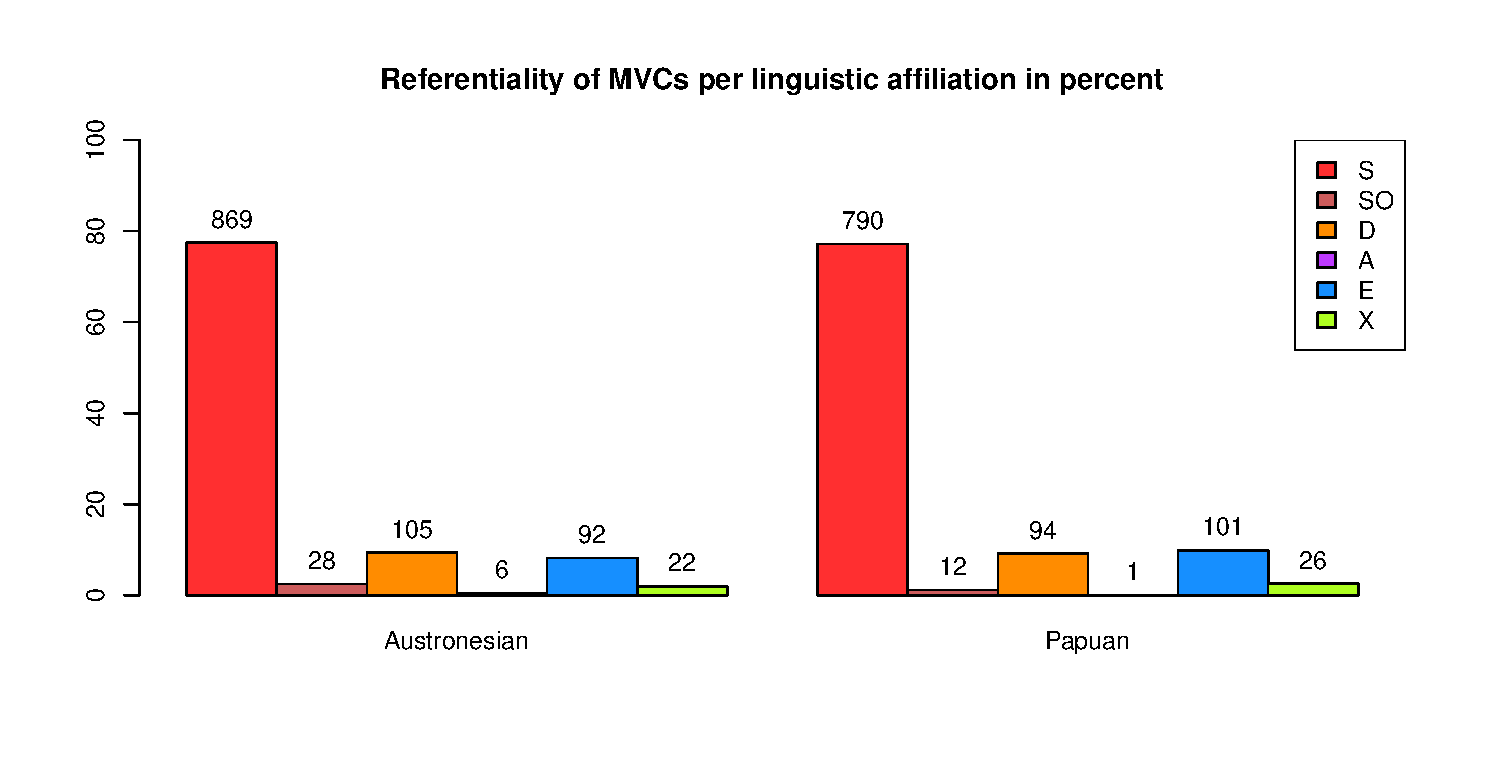
\includegraphics[width=\columnwidth]{figures/Referentiality_Family.eps}
\caption[Referentiality of MVCs per linguistic affiliation]{Referentiality of MVCs per linguistic affiliation. S = Co-functional (``same subject"), SO = Transitive co-functional (``same subject and object"), D = Switch-function (``Different subject"), A = Participant accumulation, E = Event-to-argument (``Ambient"), X = no interaction, no arguments shared. Numbers on top of the bars refer to the number of observations in the sample.}\label{fig:ref-family}
\end{figure}
\begin{figure}
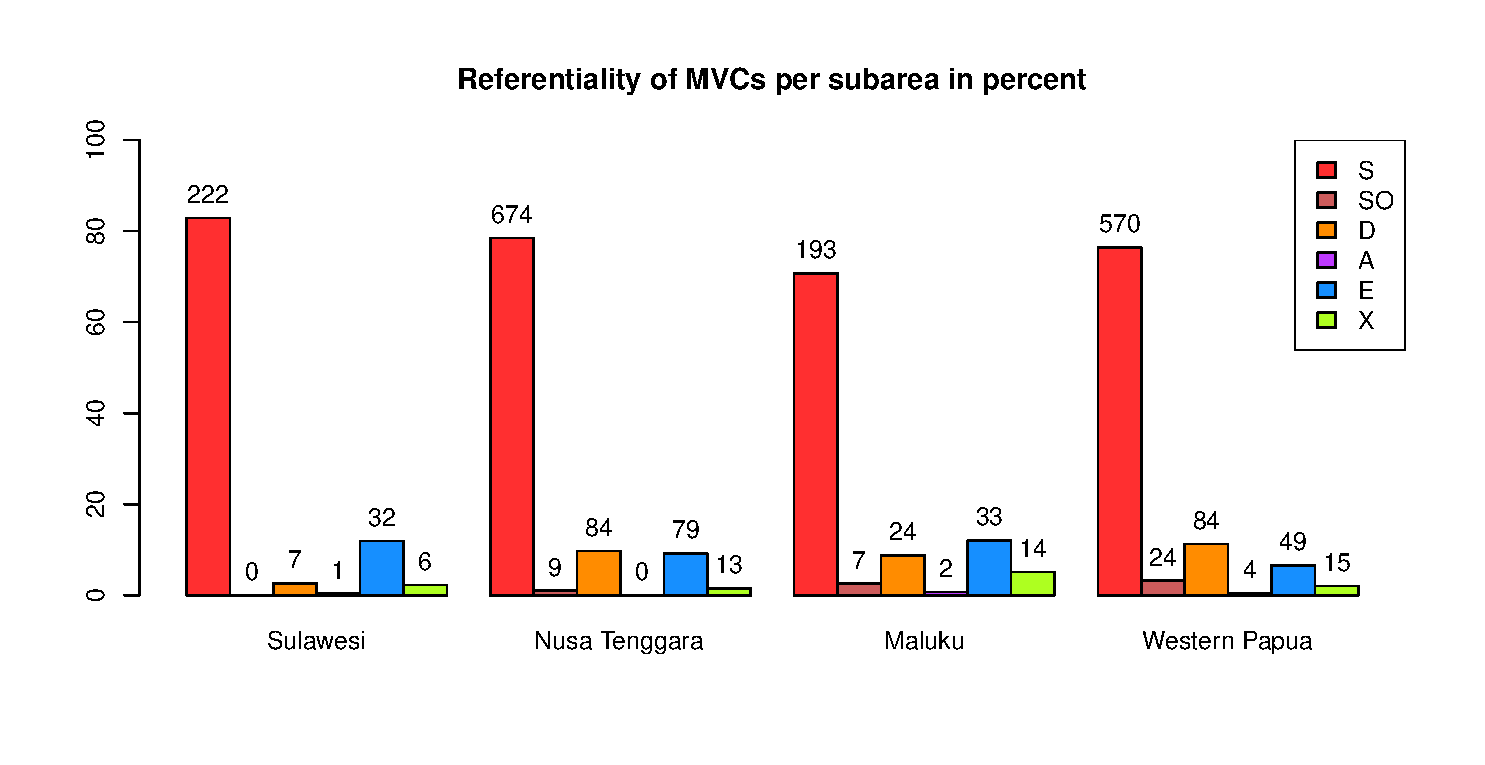
\includegraphics[width=\columnwidth]{figures/Referentiality_Group.eps}
\caption[Referentiality of MVCs per subarea]{Referentiality of MVCs per subarea. S = Co-functional (``same subject"), SO = Transitive co-functional (``same subject and object"), D = Switch-function (``Different subject"), A = Participant accumulation, E = Event-to-argument (``Ambient"), X = no interaction, no arguments shared. Numbers on top of the bars refer to the number of observations in the sample.}\label{fig:ref-group}
\end{figure}

The areal distribution patterns are quite consistent with the overall trends. \figref{fig:ref-group} again illustrates an overall similar distribution of referentiality values across subareas. Trends are hardly visible. The relation between ``D" and ``E" is subject to a certain degree of variation. While there are more ``E" than ``D" constructions in the Sulawesi and Maluku languages, Nusa Tenggara and, in particular, the Western Papua languages show the opposite pattern. Here, the ``D" pattern is more frequently encountered. Maluku also has more ``X" cases in relation to the other referentiality values than the other three groups, but this could be due to the small number of languages in this subsample (more languages might level out the overall number).

\begin{table}
\begin{tabular}{lrrrrrr}
  \lsptoprule
Language & \multicolumn{1}{c}{S} & \multicolumn{1}{c}{SO} & \multicolumn{1}{c}{D} & \multicolumn{1}{c}{A} & \multicolumn{1}{c}{E} & \multicolumn{1}{c}{X} \tabularnewline 
  \midrule
  \ili{Muna} &  39 &   0 &   2 &   0 &   6 &   3 \tabularnewline 
  \ili{Pendau} &  44 &   0 &   2 &   0 &   5 &   0 \tabularnewline 
  \ili{Tajio} &  28 &   0 &   1 &   0 &   3 &   0 \tabularnewline 
  \ili{Tolaki} &  61 &   0 &   1 &   0 &   3 &   0 \tabularnewline 
  \ili{Tukang Besi} &  50 &   0 &   1 &   1 &  15 &   3 \tabularnewline 
  \midrule
  \ili{Abui} & 100 &   0 &   1 &   0 &   5 &   3 \tabularnewline 
  \ili{Alorese} &  36 &   0 &  11 &   0 &   0 &   0 \tabularnewline 
  \ili{Bunaq} &  49 &   0 &  12 &   0 &  26 &   0 \tabularnewline 
  \ili{Kaera} &  23 &   0 &   1 &   0 &   0 &   0 \tabularnewline 
  \ili{Kambera} &  35 &   4 &   4 &   0 &   1 &   0 \tabularnewline 
  \ili{Klon} &  94 &   0 &   3 &   0 &   2 &   1 \tabularnewline 
  \ili{Makalero} &  56 &   0 &  8 &   0 &  12 &   0 \tabularnewline 
  \ili{Teiwa} &  75 &   0 &   5 &   0 &   1 &   4 \tabularnewline 
  Tetun &  61 &   0 &  12 &   0 &   0 &   0 \tabularnewline 
  \ili{Waima'a} & 115 &   5 &  23 &   0 &  29 &   4 \tabularnewline 
  Western Pantar &  30 &   0 &   4 &   0 &   3 &   1 \tabularnewline 
  \midrule
  \ili{Buru} & 51 & 0 & 1 & 0 & 16 & 0 \tabularnewline
  \ili{Selaru} &  15 &   2 &   2 &   2 &   0 &   4 \tabularnewline 
  \ili{Taba} &  29 &   3 &  9 &   0 &   3 &   0 \tabularnewline 
  \ili{Tidore} & 71 & 0 & 10 & 0 & 8 & 3 \tabularnewline
  \ili{Tobelo} &  27 &   2 &   2 &   0 &   6 &  7 \tabularnewline 
  \midrule
  \ili{Abun} &  28 &   0 &   3 &   0 &   1 &   1 \tabularnewline 
  \ili{Biak} &  48 &   6 &  7 &   2 &   3 &   1 \tabularnewline 
  \ili{Dusner} &  36 &   1 &  9 &   0 &   0 &   3 \tabularnewline 
  \ili{Hatam} &  46 &   0 &  3 &   0 &   0 &   0 \tabularnewline 
  \ili{Inanwatan} &  23 &   0 &   3 &   0 &   0 &   2 \tabularnewline 
  \ili{Maybrat} &  54 &   0 &  14 &   1 &  9 &   0 \tabularnewline 
  \ili{Mor} &  66 &   1 &   0 &   1 &   0 &  3 \tabularnewline 
  \ili{Moskona} &  39 &   0 &  16 &   0 &  24 &   0 \tabularnewline 
  \ili{Mpur} &  44 &   4 &   6 &   0 &   4 &   4 \tabularnewline 
  \ili{Sougb} &  32 &   5 &   3 &   0 &   0 &   0 \tabularnewline 
  \ili{Wooi} & 155 &   6 &  20 &   0 &   8 &   1 \tabularnewline 
   \lspbottomrule
\end{tabular}
\caption[Argument structure interaction per language]{Argument structure interaction per language. S = Co-functional (``same subject"), SO = Transitive co-functional (``same subject and object"), D = Switch-function (``Different subject"), A = Participant accumulation, E = Adverbial raising (``Event-to-argument"/ ``ambient"), X = no interaction, no arguments shared.}
\label{table:Referentiality_per_lang}
\end{table}

A look at the argument interaction patterns per language (\tabref{table:Referentiality_per_lang}) confirms the hypothesis that all languages make good use of the same subject pattern, making it the default argument sharing pattern in the EI area. A further interesting point is that virtually all languages (except for \ili{Mor}) seem to make use of the switch function (``D") interaction pattern as well, albeit often in very low numbers. Of the other patterns, ``E" is present in all subgroups and found almost all over Sulawesi, Nusa Tenggara and Maluku. Only the Western Papua languages show less usage of this type (the bulk of examples here is from only one language, \ili{Moskona}). The three other patterns are restricted to a subset of areas or even languages. ``SO" is absent from Sulawesi, and quite rare in Nusa Tenggara. Participant accumulation ``A" is virtually absent from Sulawesi and Maluku, and totally absent from Nusa Tenggara. Finally, ``X" is present in all subgroups, but only in a fraction of languages.

All in all, we may say that none of the referentiality patterns is exclusively confined to certain subareas or even to certain languages, suggesting that all patterns somehow participate in the overall dissemination of linguistic features through language contact. The fact that the ``D" pattern is in use in almost all languages would make it a particularily good candidate for an areal feature, further confirming the existence of a Sprachbund area including Sulawesi and Western Papua. This would, however, only hold true if switch function patterns could be demonstrated to be unequally distributed among serialisation languages in general. Such an assumption is difficult to validate as figures for ``D" have seldom been given. \textcite{Aikhenvald2006} and \textcite{Durie1997}, for instance, make no mention as to how many languages in fact use ``D" type SVCs in their data set. Writing on the languages of Eastern Indonesia, \citet[26]{vanstaden2008serial} state that \begin{quote}[c]o-dependent serialisation is not a very regular pattern in the East Nusantara languages. In the Austronesian languages it is only found in \ili{Taba} and in \ili{Ambon Malay}. It is more widely attested in the Papuan languages (\ili{Moi}, \ili{Mpur}, \ili{Abun}, \ili{Maybrat}) but it is never a frequent pattern.\end{quote}
We have just seen in \tabref{table:Referentiality_per_lang} that this assumption appears to be too pessimistic for Eastern Indonesia, and that a larger amount of data might result in the detection of more ``D" constructions. Note in particular that switch-function has now been attested in three further Austronesian languages, \ili{Buru}, \ili{Kambera} and \ili{Tetun Fehan}, that were also part of van Staden and Reesink's sample, but for which no examples could then be found.

The following sections provide examples from the EI languages and discuss some peculiarities related to the different patterns. The sections are sorted into argument sharing and no-argument sharing patterns.

\subsection{Argument sharing}

MVCs with argument sharing amount to 1905 cases (out of 2146) in the EI sample. This means that argument sharing in general can be regarded as a core trait of MVCs, and is highly predictable. All three argument sharing types have in common some relation of shared identity between the arguments of different verbs. Co-functional MVCs, that is, the ``S" and ``SO" patterns, maintain a single syntactic function, whereas switch-function MVCs and participant accumulation MVCs do not.

\subsubsection{Co-functional MVCs}

Co-functional MVCs occur in all EI languages. As this is the default type, I will not have much to say about it. The following examples are from the four subareas, and are chosen to show different degrees of verbal subject encoding: both verbs may be closely strung together and share one set of affixes, as in example (\ref{tukangbesi003}) from \ili{Tukang Besi}; both verbs may remain completely uninflected (\ili{Klon} example); both verbs may be inflected for a shared subject referent, as in the \ili{Tobelo} example in (\ref{tobelo001}); or only the first verb may be inflected for subject whilst the second remains bare (\ili{Hatam}). Whatever the coding option, the common ground in all these constructions is that each verb refers to the same subject referent. So, for instance, in example (\ref{tukangbesi003}) the subject referent denoted by \textit{no-} is understood as being licensed by both \textit{wila} and \textit{ako}.

\ea \label{tukangbesi003}
\langinfo{Tukang Besi}{Austronesian, WMP}{\citealt[201]{donohue1999}}\\
\gll no-wila-ako-'e (na ina-no) kua daoa \\
3\textsc{rls}-go-do.for-3\textsc{obj} \textsc{nom} mother-3\textsc{poss} \textsc{all} market \\
\glft `They went for their mother to the market.'\\ 
\z

\ea 
\langinfo{Klon}{Papuan, TAP}{\citealt[137]{baird2008grammar}}\\
\gll kuur angkol a-awar qad alah mi ik \\
dog self \textsc{rdp}-return come house be.at \textsc{compl} \\
\glft `The dog itself came back and was at home.'\\ 
\z

\ea \label{tobelo001}
\langinfo{Tobelo}{Papuan, NH}{\citealt[43]{holton2003tobelo}}\\
\gll o-Morotai-iha gaanga yo-koki-boa yo-karajanga \\
\textsc{nm}-M.-\textsc{land} there 3\textsc{pl}-\textsc{dstr}-come 3\textsc{pl}-work \\
\glft `We all came to Morotai to work.'\\
\z

\ea 
\langinfo{Hatam}{Papuan, \ili{Hatam}-Mansim}{\citealt[108]{reesink1999grammar}}\\
\gll yoni y-ug bong ei ig-bei big \\
they 3\textsc{pl}-go sleep \textsc{loc} house-under not \\
\glft `They don't go (to) sleep in the house (at home).'\\ 
\z

The most common sharing pattern is subject sharing, as we have seen. In case there are objects, these are often not shared (two examples for object sharing are given below; further discussion is found in \sectref{sec:handling-to-action} on handling constructions that involve both ``S" and ``SO" patterns). Object sharing is also much rarer than subject sharing as many verbs in V$_1$ position are intransitive (as is the case with the motion verbs in the examples above). This may, for instance, explain why the Sulawesi languages have no ``SO": there are hardly any combinations of transitive verbs found. When object sharing does take place in the other subareas, it always seems to involve subject sharing as well. Both verbs in such cases are of course transitive. V$_1$ more or less invariantly involves a verb of object manipulation (basically verbs of taking, and patientive manipulation verbs such as hitting, kicking, stabbing or hammering). Here are two examples of object sharing:

\ea \label{taba001}
\langinfo{Taba}{Austronesian, SHWNG}{\citealt[311]{bowden2001taba}}\\
\glll ntotas nik kos nabulang \\
n=totas nik kos n=ha-bulang \\
3\textsc{sg}=wash 1\textsc{sg}.\textsc{poss} T-shirt 3\textsc{sg}=\textsc{caus}-be.white \\
\glft `She washed my T-shirt white.'\\ 
\z

\ea \label{mpur001}
\langinfo{Mpur}{Papuan, isolate}{\citealt[98]{ode2002sketch}}\\
\gll n-soro mar ka n-da(k)-frak nton aka ut \\
3\textsc{sg}.\textsc{f}-take.off cloth that 3\textsc{sg}.\textsc{f}-take-throw child then died \\
\glft `She took off that cloth and threw the child away and it died.'\\ 
\z

Example (\ref{taba001}) from \ili{Taba} is a resultative construction in which a causative verb is derived from a resultant state verb, sharing the object with the first verb, \textit{nik kos} `my T-shirt' (a more literal translation would probably be `she washed my T-shirt$_i$ causing it$_i$ to become white'). The second example in (\ref{mpur001}) is from \ili{Mpur}, and shows a close combination of a \textsc{take} verb and a \textsc{throw} verb. Both verbs are transitive and license both a co-referential subject and object argument (`and took (and) threw the child away' would probably be more precise).

\subsubsection{Switch-function MVCs}

Switch-function MVCs are found in all EI languages but one (I am assuming that the missing data from \ili{Mor} are most probably a chance effect). The canonical switch-function type is similar to the shared subject and object constructions (``SO") from the last section in that an event of object manipulation is viewed from two different perspectives. In the SO type, both event designators assume an agentive perspective, just as in example (\ref{mpur001}) from \ili{Mpur} (actor does action A to object$_i$, actor does action B to object$_i$). The only difference in the switch-function type is that it is only the first event designator that is agent-oriented. The second verb then shifts to an undergoer perspective with the \textsc{patient} entering into subject function. Such MVCs most often express a \textsc{cause-result} or a causative relation. \citet{crowley2002serial} refers to this types as switch-subject serial verbs, and gives the following oft-cited example from \ili{Paamese}:

\ea 
\langinfo{Paamese}{Austronesian, Oceanic}{\citealt[55]{crowley2002serial}}\\
\glll inau nuas vuas he:mat \\
inau ni-uasi vuasi hee-mate \\
1\textsc{sg} 1\textsc{sg}:\textsc{dist}.\textsc{fut}-hit pig 3\textsc{sg}:\textsc{dist}.\textsc{fut}-die \\
\glft `I will hit the pig to death.'\\ 
\z

The EI languages use the switch-function pattern a lot for constructions involving a causing action and a resulting action or state. In \ili{Biak}, for instance, all ``D" cases are annotated as being related to some sort of causation. The following one is rather typical: the process of a glass breaking due to some involuntary action is split up into two event kernels: the agent incidentally strikes the glass (the object), and the glass (now being understood as subject of the second, intransitive verb \textit{kpéf}) shatters.

\ea 
\langinfo{Biak}{Austronesian, SHWNG}{\citealt[194]{vanheuvel2006}}\\
\glll yúf mnis gelas ine va vo, yamer kpéf i \\
y-úf mnis gelas i-ne va vo ya-mer kpéf i \\
1\textsc{sg}-take fit glass 3\textsc{sg}.\textsc{spec}-this not \textsc{sim} 1\textsc{sg}-strike.hard shatter 3\textsc{sg} \\
\glft `I did not pick up the glass rightly so that I struck and made it shatter.'\\ 
\z

Similar construals appear in many other EI languages. The agent of V$_1$ may in some cases be replaced by the instrument as such, carrying out the action, as in example (\ref{bunaq001}) from \ili{Bunaq} where the machete is promoted to subject function. Here the resultant event is not expressed by a state change verb but by a stative verb, rendering it a resultative construction rather than a construal with two active verbs.

\ea \label{bunaq001}
\langinfo{Bunaq}{Papuan, TAP}{\citealt[447]{schapper2009bunaq}}\\
\gll Sore rebel, gu-bul bere pak tol haqal. \\
machete descend 3\textsc{an}-head \textsc{cntrexp}.\textsc{inan} strike broken finished \\
\glft `The machete descended (and) struck his head splitting it completely.’\\ 
\z

Example (\ref{maybrat001}) from \ili{Maybrat} below illustrates another quite freqent pattern, this time with a \textsc{theme} object becoming the subject of V$_2$ in what I call \textsc{direction complex} constructions (see discussion in \sectref{sec:direction}). Literally, it would mean `Should I pour water go(es) into the thermos flask'.

\ea \label{maybrat001}
\langinfo{Maybrat}{Papuan, isolate}{\citealt[215]{dol2007grammar}}\\
\gll t-tu aya m-amo cerek a \\
1\textsc{sg}-pour water 3\textsc{u}-go thermos.flask \textsc{int} \\
\glft `Should I pour water into the thermos flask?'\\ 
\z

The switch-function concept also extends to other construction types that seem less widespread and much more specific. Example (\ref{abui003o}) from \ili{Abui} illustrates a case where a quantifier verb \textit{tafuda} is interpreted to have a subject that is co-referential with the direct object of the main verb \textit{fur} (something like `he swallowed it$_i$ (it$_i$ is) all'). Note that (\ref{abui003o}) is one of very few cases in which the function switch seems to occur the other way round: it is not the object of V$_1$ that is reanalysed as subject of V$_2$, but V$_2$ has a direct object that is reanalysed as subject of V$_1$. This order is in the \ili{Abui} case an effect of general rules of constituent order placing the main verb(s) last in the clause.\footnote{Unfortunately, I have hardly found any further data that would allow to expand on this issue. What seems to be going on is that there is a clash of two constraints on constituent order at work in (some) AOV languages. On the one hand, AOV languages prefer to place the main verb at the end of the construction (just as clause-chaining languages would place their final verb at the end of the chain). On the other hand, there is a general preference in MVCs to place the verbal constituents according to the sequence in which the event stages occur (principle of iconicity; see for instance \citealt{vanstaden2008serial}). As we will see in \sectref{sec:causation}, these constraints appear to interact in complex ways, and the outcome is not always predictable. In cause-result MVCs from AOV languages, for instance, temporal iconicity is sometimes preserved, and sometimes overwritten.} Cases of reversed switch-function have therefore been subsumed under the label ``D". Another reason was that the number of instances was at any rate not sufficient to argue for a referential interaction type of its own.

\ea \label{abui003o}
\langinfo{Abui}{Papuan, TAP}{\citealt[372]{kratochvil2007grammar}}\\
\gll tafuda ha-fur-i he-nil-e \\
be.all 3\textsc{pat}-swallow.\textsc{compl}-\textsc{prfv} 3\textsc{loc}-make.like.this-\textsc{ipfv} \\
\glft `He swallowed everything this way.’\\ 
\z

The \ili{Abui} example illustrates MVCs in which the function switch is only implicit, and no morphology helps interpret the argument relations. In other languages, subject marking does, in principle, allow for reference tracking, but function switches between third person referents may frequently occur along the way within concatenations of verbs. This is often only indicated by the semantic context. Take the \ili{Muna} example in (\ref{muna0016}) which is, with four verbs in sequence, exceptionally long for a Sulawesi MVC. Between the first verb and the second is a function switch: it is the old man that is with a stick, not the female actor from V$_1$. V$_3$ and V$_4$ then continue with the old man being the subject. Note that the indirect object suffix of the first verb refers to \textit{kamokula}, the old (man).

\ea \label{muna0016}
\langinfo{Muna}{Austronesian, WMP}{\citealt[241]{vandenberg1989}}\\
\gll no-po-ghawa-ghoo kamokula ne-katuko no-mai-ghoo no-hulo \\
3\textsc{sg}.\textsc{rls}-\textsc{recp}-meet-\textsc{io} old 3\textsc{sg}.\textsc{rls}-stick 3\textsc{sg}.\textsc{rls}-come-\textsc{io} 3\textsc{sg}.\textsc{rls}-hunt \\
\glft `She met an old man with a stick who had been hunting.'\\ 
\z

\subsubsection{Participant accumulation}

Participant accumulation, as we have seen, is rather not a typical case of argument sharing because the referent of V$_2$ is not identical with either the subject or the object of V$_1$. Rather, it is the sum of both the subject and the object referent. This entails that V$_1$ is either transitive or intransitive with a second oblique argument. In the EI languages, two ways of construing participant accumulation can be distinguished. The \ili{Paamese} type from example (\ref{paamese003}) involves a \textsc{take} verb, followed by some joint action (`I take you, we go'). The EI examples differ from this pattern in that V$_1$ (or a nested MVC in the first slot of the matrix construction) denotes a motion event (like `you come (to me), we do' or `I take you here, we do'). This motion component seems to be absent in the \ili{Paamese} construction. An alternative pattern is the use of a comitative function verb in V$_1$, yielding something like `I with you, we do'. The following examples from \ili{Tukang Besi} and \ili{Selaru} illustrate both options. Note that, strictly speaking, it is not clear in examples like (\ref{tukang003}) that the motion verb assigns a human goal argument in the first place. Alternatively, \textit{mai} might only vaguely imply a spatial origo, which, by implicature, is interpreted as being the location of the first person singular participant. In any case, participant accumulation is a rare phenomenon in EI, and clearly different from default \ili{Paamese} participant accumulation.

\ea \label{tukang003}
\langinfo{Tukang Besi}{Austronesian, WMP}{\citealt[516]{donohue1999}}\\
\gll Mai to-wila-ako to-tunga-ntunga, La bela Kandokendoke. \\
come 1\textsc{pl}.\textsc{rls}-go-\textsc{appl} 1\textsc{pl}.\textsc{rls}-\textsc{red}-fish La dear Monkey \\
\glft `Let's go and do some fishing, Dear Monkey.'\\ 
\z

\ea \label{selaru001o}
\langinfo{Selaru}{Austronesian, CMP}{\citealt[120]{coward2005}}\\
\gll Y-aso sir ma r-al-a kotw ti enen desike y-or amam desike ra ma ktei. \\
3\textsc{sg}-request them \textsc{conj} 3\textsc{pl}-give-Ø food \textsc{conj} woman that 3s-with man that they.eat until done \\
\glft `He requested they give the food so that woman and that man [can] eat until done.'\\ 
\z

\subsection{No argument sharing}

MVCs without argument sharing come in two types. The first type is annotated as ``E", marking cases where the whole first VP is reanalysed as an impersonal subject referent of the second verb. The second type appears to feature two or more VPs that have no connection to each other whatsoever. This type has been labelled ``X". Both types contribute a total of 241 cases to the sample.

\subsubsection{Event-to-argument reanalysis}\label{sec:event-to-argument}

Event-to-argument reanalysis typically consists of two event kernels: an action event, and a modifying or evaluative state. The action event becomes the sole argument of the evaluative state. Event-to-argument reanalysis is an obvious feature only in those languages that use subject indexing morphology on the verb. Languages without verbal morphology do not offer direct clues for an event-to-argument relation in MVCs but certain construction types can be interpreted that way (though not uncontroversially, or so it seems). Let us begin with some examples from languages that do mark this type. \ili{Maybrat}, for instance, has a smallish class of prepositional verbs. Two of these verboids, \textit{ae} `be at' and \textit{kah} `be with', occur in MVCs where their subject does not agree with the subject of the action verb. Rather, it shows the prefix for third person unmarked gender. Compare the following examples.

\ea \label{maybrat002}
\langinfo{Maybrat}{Papuan, isolate}{\citealt[80]{dol2007grammar}}\\
\ea
\gll ait y-amo m-ae amah \\
he 3\textsc{m}-go 3\textsc{u}-at house \\
\glft `He goes home.' \\ 
\ex
\gll ait y-amo y-ae amah \\ 
he 3\textsc{m}-go 3\textsc{m}-at house \\
\glft `He goes and he is at home.'\\ 
\z
\z

\newpage

\ea \label{maybrat003}
\langinfo{Maybrat}{Papuan, isolate}{\citealt[80]{dol2007grammar}}\\
\ea
\gll t-ai m-kah ara \\
1\textsc{sg}-hit 3\textsc{u}-with stick \\
\glft `I hit with a stick.' \\ 
\ex
\gll *t-ai t-kah ara \\ 
1\textsc{sg}-hit 1\textsc{sg}-with stick \\
\z
\z

The first pair in (\ref{maybrat002}) shows two ways of using the verboid \textit{ae} with a motion verb in V$_1$. It may either agree in person marking with the motion verb, yielding a motion event with successive event stages (the going, and the resultant being at the place of destination), or it may show a disagreement in person marking. In this case, as there is no other participant available that \textit{m-} could refer to, I would suggest that it represents an instance of event-to-argument reanalysis. Semantically, one could expect something like `the going of him is (directed) at the house'. The free translation given by Dol suggests that both verbs together are interpreted as denoting one single motion event (as opposed to the staged example with person marking agreement). A similar case is found with \textit{kah} in (\ref{maybrat003}) except that the event-to-argument construal is the only one permitted. Here as well, my interpretation is that it is the hitting that \textit{m-} refers to (`my hitting is with a stick').

Other contexts with event-to-argument construals pertain to adverbial \textsc{modification}. In \ili{Tukang Besi} and \ili{Muna}, adverbials may behave like full verbs in that they receive subject indexing morphology. Yet in many cases, no real participant is selected but the subject indexer seems to refer to the whole event which is modified. Consider the example pair from \ili{Muna} below.

\ea \label{muna003}
\langinfo{Muna}{Austronesian, WMP}{\citealt[236f.]{vandenberg1989}}\\
\ea
\gll no-nea a-leni \\
3\textsc{sg}.\textsc{rls}-usual 1\textsc{sg}.\textsc{rls}-swim \\
\glft `I usually swim.' \\ 
\ex
\gll ao-nea a-leni \\ 
1\textsc{sg}.\textsc{rls}-usual 1\textsc{sg}.\textsc{rls}-swim \\
\glft `I usually swim.' \\ 
\z
\z

The two ways of construing a temporal modification in (\ref{muna003}) offer an interesting contrast in argument relation. In the first construction, ``the juxtaposed clause is semantically the subject of the first clause", according to \citet[236]{vandenberg1989}. With some such adverbial verbs, however, a second construal is possible where the subject indexer of the modifying verb agrees with the subject of the main verb. This phenomenon is called subject harmonisation by van den Berg. Some adverbial verbs always require subject harmonisation, others never do, and a third group allows optional subject harmonisation, as for instance with \textit{nea} `(be) usual'.

All the instances above quite clearly encode event-to-argument reanalysis. In languages without rigorous subject marking on the verb, however, such construals are often only indirectly inferable. In the following examples, one of the verbs seems to refer to the whole VP rather than to a concrete participant, but this is a matter of interpretation and not marked by grammatical means.

\ea \label{abui003}
\langinfo{Abui}{Papuan, TAP}{\citealt[363]{kratochvil2007grammar}}\\
\gll di=ng wahai mara \\
3\textsc{act}=see look go.up.\textsc{cont} \\
\glft `He looks up.’\\ 
\z

\ea 
\langinfo{Taba}{Austronesian, SHWNG}{\citealt[315]{bowden2001taba}}\\
\glll Lkiu kwat \\
l=kiu kwat \\
3\textsc{pl}=be.frightened be.strong(\textsc{emph}) \\
\glft `They were really frightened.' \\ 
\z

\ea \label{waimaqa007}
\langinfo{Waima'a}{Austronesian, CMP}{dom2\_kaben 219f.}\\
\gll nau hite ma'a lo, den te ma'a lo \\
know \textsc{ptl} finish \textsc{asp} hear \textsc{ptl} finish \textsc{asp} \\
\glft `(You) already know, have already heard (...)'\\ 
\z

Example (\ref{abui003}) illustrates a construal of visual perception with a path specification denoted by a directed motion verb. As a simplex predicate, \textit{mara} `go up' would license an actor, yet the MVC in (\ref{abui003}) already has an actor (which is the experiencer, introduced by the grammaticalised element \textit{=ng}). Since the context makes it clear that the experiencer is not moving upward, the best interpretation would be that the whole event of him looking is directed upwards. The next example from \ili{Taba} is a similar case. \textit{Kwat} can be an independent verb in simplex predicates. Here, it seems that the event of them being frightened is taken to be the argument of \textit{kwat} (`their being frightened is strong'). The last example in (\ref{waimaqa007}) is a completive construction from \ili{Waima'a}, involving the verb \textit{ma'a} that is sometimes glossed as `finish' and sometimes as `all'. As knowing and hearing are non-agentive events and no agent seems available in both MVCs, \textit{ma'a} could again be interpreted as taking the whole event as its single argument (the knowing is all/complete/finished)\footnote{It seems tempting to analyse such \textsc{finish} verbs the ``\ili{English} way" as syntactically transitive verb. However, \textsc{finish} verbs in EI languages typically do not offer any clue as to their transitivity.}.

In \ili{Buru} we find an intruiging example of what seems to be an event-to-ar\-gu\-ment reanalysis together with normal subject sharing. \ili{Buru} offers an interesting contrast in object marking with completive MVCs. The object enclitic \textit{-h} may either attach to the matrix verb (as in example (\ref{Buru4}) below), or to the completive verb (cf. example (\ref{Buru5})). The former case seems to highlight the consumption of the item, and \textit{sepo} could be taken as showing an unmarked same subject pattern (`he ate-it (he) finished'). This case is best described as a completive construction. A more apt translation of example (\ref{Buru4}) would thus be `He ate it all'. The latter case, on the other hand, appears to reanalyse the eating process denoted by V$_1$ as its direct object (`he ate (he) finished-it' where `it' would refer back to the eating).\footnote{Alternatively, the second constructions could be analysed as a plain affix-sharing nuclear-layer construction, with \textit{-h} still referring to the object licensed by the main verb. This would, however, not directly explain the specific focus in meaning on the action.} If that were so, we would be dealing with two argument-sharing devices being active within one MVC: same subject would allow sharing the subject referent, while the object of V$_2$ would be available through event-to-argument reanalysis. Note that such an interpretation would at any rate differ from canonical cases of ``E" in that the main event is not reanalysed as the subject of an unaccusative V$_2$, but rather as the object of a transitive verb in V$_2$. 

\ea 
\langinfo{Buru}{Austronesian, CMP}{\citealt[160]{grimes1991buru}}\\
\ea \label{Buru4}
\gll da kaa-h sepo \\
3\textsc{sg} eat-\textsc{obj}.\textsc{sg} finish \\
\glft `He finished eating it. (consumption of item)' \\ 
\ex \label{Buru5}
\gll da kaa sepo-h \\ 
3\textsc{sg} eat finish-\textsc{obj}.\textsc{sg} \\
\glft `He finished eating it. (completion of action)'\\ 
\z
\z

As this brief discussion has shown, assigning the label ``E" to MVCs is a matter of interpretation in languages that do not offer direct morphosyntactic reference tracking on the verb. Therefore it should be borne in mind that the numbers for ``E" MVCs presented in this study might change under closer investigation of the underlying referential systems.

\subsubsection{Cases without argument interaction}

MVCs without any argument interaction cover a range of constructions, and can be found in most of the EI languages. Many cases involve what seems to be juxtaposed clauses without prosodic boundary cues. Prosodic units that are uttered in close succession without clear rhythmical boundary cues are known as latching in prosody research (cf. for instance \citealt{himmelmann2018}). However, the MVCs without argument interaction that I have found in the literature are more than just prosodic collocations that reflect rapid prosodic production. In most of the cases, both (or all) events encoded by the verbs are related to each other in certain recurring ways. This relation may be temporal in that both events occur simultaneously, or in explicit sequence.  Consider for instance the simultaneous construal of the verbs \textit{hupu} and \textit{tiha} from \ili{Tobelo} below.

\ea 
\langinfo{Tobelo}{Papuan, NH}{\citealt[61]{holton2003tobelo}}\\
\gll to-hupu-óko ahi-kongo i-tiha \\
1-go.out-\textsc{sea} 1\textsc{poss}-tears 3-fall \\
\glft `I came out with tears falling.'\\ 
\z

Other cases rather denote conditional relations, as in example (\ref{muna004}) from \ili{Muna}. Cases like this may turn out to be simple biclausal conditionals where the grammatical marker can be left out (as with \textit{ane}). Van den Berg notes that ``it is possible to add a conjunction (for example \textit{ane} `if'), which results in a conjoined construction" \citep[235]{vandenberg1989}.

\ea \label{muna004}
\langinfo{Muna}{Austronesian, WMP}{\citealt[235]{vandenberg1989}}\\
\gll nao-kesa sepaliha dua suara-no (ane) nae-lagu \\
3\textsc{sg}.\textsc{irr}-beautiful very also voice-his (if) 3\textsc{sg}.\textsc{irr}-sing \\
\glft `His voice will also be very beautiful when he sings.'\\ 
\z

\section{Constituent structure}

The next sections now turn to morphosyntactic features on the level of constituent structure. Differences in grammatical marking between the verbs of a MVC have led many to postulate differences in constructional make-up. For instance, van Staden and Reesink classify SVCs with two inflected verbs into one category, and SVCs with only one inflected verbs into another. \sectref{sec:headedness} presents an overview of inflection patterns in the EI sample, and aims at discussing the theoretical implications that these patterns may have. One way of analysis would treat inflected verbs as conceptual heads of a syntactic projection, leading in the case of van Staden \& Reesink's ``dependent type" to a potentially hypotactic construction with one verbal constituent being of higher rank than the other. An alternative approach would not grant verbal inflection the status of a head-marking device in the sense that the underlying construction would necessarily be interpreted as hypotactic. While I will argue for some structural difference between inflected and uninflected verbs, my point is that the majority of languages from the area does not explicitly use verbal morphology to systematically trace hierarchical differences in MVCs. At the same time, certain MVCs indeed carry an inflection pattern that seems induced by the construction rather than by some parameter from other linguistic planes (such as phonology).

The second parameter discussed here under the label \textit{constituent structure} is contiguity of verbal constituents. As mentioned before, contiguity (or adjacency) of verbs is another factor often recognised as being vital to SVC formation, and construction types are often said to be sensitive to strict contiguity (think again of Pawley's compact serialisation type, for instance). \sectref{sec:contiguity} will discuss contiguity in EI MVCs.

\subsection{Headedness}\label{sec:headedness}

Verbal inflection highlights the verb as being of central importance to the construction in question, or, in Bloomfield's terms, being the \textit{center} of the construction \citep{bloomfield1933language}. This central constituent is usually referred to as \textit{head}. The idea of heads in linguistics has been in use at least since Leonard Bloomfield and the American structuralist times, and, as Zwicky in his seminal paper from 1985 showed, has come with a range of different interpretations and theoretical tenets \citep{zwicky1985heads1}. 

This section proceeds as follows: I will first give a brief summary of Zwicky's account of heads, basically because he was the first to make explicit a set of competing notions that can be taken as candidates for the concept. The headedness discussion at that time was basically revolving around the \textsc{SAE} language type, with \ili{English} being the example of choice. The formula was ``one clause, one (verbal) head", and few problems arose with European languages as they adhere quite well to that principle by employing verbal morphology for finiteness distinctions in a regular way. MVCs seem to be quite different. Nevertheless it is, I think, worthwhile to take the idea of heads and apply it to these structures. In order to do so, I will in \sectref{sec:unreliable} briefly review what I call unreliable inflection in EI languages. The third part of the section in \sectref{sec:wooicase} then turns to subordinate relative clauses in \ili{Wooi}. \ili{Wooi} relative clauses are connected to the matrix clause via two marking strategies involving differential inflection patterns. I will argue that this distinction is not a finiteness distinction of the sort required for judging head marking patterns but quite a different technique driven by constraints in argument tracking. The fourth and final part of this section returns to EI MVCs and their inflection patterns, and gives examples from different languages of the sample.

\subsubsection{Zwicky: Competing concepts}\label{sec:Zwicky}

Discussing the ambiguity of the term \textit{head}, Zwicky singled out three notions that all share the basic idea that within a given set of two components, one of them is more central and characteristic of the whole constituent. These notions are: the semantic argument (later called base in \citealt{zwicky199313}), the subcategorisand (semantic functor), and the morphosyntactic locus (later called head, as this is assumed to be the most appropriate candidate notion with regard to syntactic constituency; \citealt[3]{zwicky1985heads1}). The semantic argument relies on semantic tests: the semantic head of two elements is the one element that is of the same kind as the categorial projection of both elements.

\begin{quote}
[I]n a combination X + Y, X is the `semantic head' if, speaking very crudely, X + Y describes a kind of the thing described by X. On this basis, N is the semantic head in Det + N (\textit{those penguins} describes a kind of penguin), and VP is the semantic head in Aux + VP (\textit{will leave} describes a kind of leaving). \citep[4]{zwicky1985heads1}
\end{quote}

The subcategorisand, the second candidate for the head of a constituent, is a constituent that is restricted in its ability to occur in specific constructional slots. The most prominent instance is verbs that are subcategorised with regard to the constellation of argument positions. Zwicky gives the following examples:

\begin{quote}
The verb \textit{give} is subcategorized to occur with either NP NP or NP \textit{to} + NP as its sisters (\textit{give Kim money, give money to Kim}); \textit{donate} is subcategorized to occur only in the second of these two constructions (*\textit{donate Kim money, donate money to Kim}). \citep[5]{zwicky1985heads1}
\end{quote}

The third notion of head is the morphosyntactic locus, that is, the constituent that bears the marks of morphosynactic relation to other constituents. If, for instance, a verb (or its projection, a VP) bears marks of mood or subject agreement then it is the morphosyntactic locus of the clause. Yet, this is only one of two possible understandings of \textit{morphosynactic locus}. There is another interpretation available in which the morphosyntactic locus is on all those constituents that would \emph{potentially} bear the respective inflectional marks if the language in question has developed the appropriate morphology. Thus, not only inflecting languages would have heads but also isolating languages where the potential locus is inferable from general theory.

\begin{quote}
This is a general notion of morphosyntactic locus which is to be considered as an explication of headship in syntactic theory. The actual inflectional locus will serve as a guide to the morphosyntactic locus in specific cases, at least in languages with sufficiently rich inflectional morphology. Speaking very loosely, the morphosyntactic locus is the `potential inflectional locus', the constituent on which inflectional features will be marked if the language has the appropriate morphology. \citep[6]{zwicky1985heads1}
\end{quote}

The surface-structural interpretion of heads as morphosyntactic loci of grammatical information clearly offers the most practical starting point for typological comparison, at least in languages with overt morphology. Within the serialisation debate, claims have been made as to where the locus of inflection should go in serial verb constructions. One of the most widely read (and cited) papers on this is Durie's \textit{Grammatical structures in verb serialization} with a critical evaluation of such predictions from GB approaches (\citealt{Durie1997}; mostly focusing on Baker's indirect $\theta$-marking account). What is interesting to us at this point is that Baker indeed assumed inflected verbs in SVCs to be heads:

\begin{quote}[I]t is known that only the head of a phrase can in general carry inflectional features that originate with an element outside that phrase. Interestingly, in some serializing languages the same tense/aspect and subject agreement morphology appears on every verb in the SVC. [...]  This is exactly what the theory expects. Traditionally, tense/aspect features are copied from the lnfl node onto the head of the associated verb phrase. The fact that these features show up on both verbs in the SVC thus supports the hypothesis that both verbs are heads. \citep[523f.]{baker1989object}
 \end{quote}
 
Baker's hypothesis would require one to interpret inflection as a marker of headedness in SVCs. There are different problems associated with this. First, as we have seen in Chapter \ref{ch:area}, the languages from EI encode quite different concepts on their verbs. Would TAM-morphology on verbs in Sulawesi languages then be comparable to person indexing verb morphology in languages from Western Papua? Some TAP languages even show traces of both verbal categories, TAM and person indexing. At the same time, many of these languages have restrictions on verb inflection. This leads to a second challenge: are languages with unstable verb morphology also to be analysed as marking heads? And third, how can we deal with differences in verbal inflection across different types of constructions? Is it the construction that sets the scene, for instance, by prohibiting inflection of V$_2$, or could it be that V$_2$ has become a non-verbal item, say, a directional particle or a case-marker.

The first challenge is hard to overcome. While TAM-morphology may be seen as some kind of ``canonical inflection type" (cf. \citealt{foley2010events}), the inflectional systems found in SAE languages often also include person indexing, typically involving portmanteau morphemes bundling together different conceptual categories. In a typological study such as the present one, at least two strategies are available: first, one could only compare languages with ``identical" conceptual categories encoded on the verbs. This would leave us with TAM-languages such as \ili{Tajio} and \ili{Pendau} on the one hand, and person indexing languages on the other, like most of the remaining EI languages in the sample. Obvious problems would emerge, however, with languages that do both (\ili{Inanwatan} would be a good example of a language combining tense marking with person indexing on its verbs). The second strategy would lump together languages with different verbal categories, on the assumption that as long as there is \emph{some} category encoded on the verbs we are dealing with a ``head".\footnote{Specific problems would arise in case different categories were marked on different verbs. There is, however, only one such case in the EI sample. In \ili{Abui}, aspectual suffixes always go with the final verb, while O crossreference is applied to those verbs that are lexically specified for marking undergoer arguments. This can lead in some cases to two verbal categories, marked on different verbs. For the reasons discussed in the following section neither verbal category has been interpreted as assigning head properties in \ili{Abui}. See also \sectref{sec:asymmetrical} below.} As this strategy would help avoid the above mentioned problem of deciding what to do with mixed inflectional systems, I decided to side with the lumpers rather than with the splitters, although there are obvious shortcomings with this decision. 
 
\subsubsection{Unreliable verb morphology} \label{sec:unreliable}

Let us turn to the second challenge by having another look at irregular verb-morphological systems in EI. In both the Sulawesi and Nusa Tenggara groups, a considerable portion of languages does have inflection on their verbs, but only within a subset of cases. From the introduction to the EI languages in Chapter \ref{ch:area}, we can discern three main types of unreliable inflection in EI languages: lexically determined, situationally determined or phonologically determined. To these types, we may add a fourth one, which is totally optional inflection, as found in \ili{Tidore}. This section presents a short review of these types. \tabref{table:unreliable} sums up their basic properties.

\begin{table}
\begin{tabularx}{\textwidth}{l p{4.7cm} Q}
  \lsptoprule
Type & Properties & Languages \tabularnewline 
  \midrule
Lexical & Only a subset of verbs takes inflection &  \tabularnewline \tablevspace
a) obligatory & Obligatory inflection of verbs in subset & \ili{Tajio}, \ili{Pendau}, \ili{Teiwa}, \ili{Makalero} \tabularnewline
\tablevspace
b) optional & Optional inflection of verbs in subset & \textit{not attested, but see below} \tabularnewline
\tablevspace
c) mixed & subclasses of verbs with obligatory and optional inflection & Western Pantar, \ili{Kaera}, \ili{Klon}, \ili{Bunaq} \tabularnewline
\midrule
Situational & Properties of the NP determine whether or not person indexer appears on the verb & \tabularnewline
\tablevspace
a) definiteness & indefinite NPs prevent inflection & \ili{Kambera} \tabularnewline
\tablevspace
b) specificity & non-specific NPs prevent inflection & \ili{Abui} \tabularnewline
\tablevspace
c) animacy & inanimate NPs prevent inflection & Western Pantar, \ili{Teiwa}, \ili{Bunaq} \tabularnewline
\midrule
Phonological & Phonological factors delimit inflection & \ili{Tetun Fehan}, \ili{Alorese} \tabularnewline
\midrule
Free & Inflection completely optional & \ili{Tidore} \tabularnewline
   \lspbottomrule
\end{tabularx}
\caption[Types of unreliable inflection in EI languages]{Four types of unreliable inflection in the EI sample. Some languages are assigned two categories as they exhibit properties of both types. See \sectref{introlang} for information on the languages, and their verbal systems.}
\label{table:unreliable}
\end{table}

The first type, the lexical type, is most widespread and covers both the \textsc{sul} and the \textsc{nus} subgroups, albeit within quite different configurations. While the Sulawesi languages \ili{Tajio} and \ili{Pendau} have a very small class of directional verbs resisting inflection, the opposite is true for some of the Nusa Tenggara languages where the subset of verbs that do take inflection seems quite small (\ili{Makalero}) or cannot be estimated from the publications (for instance, \ili{Teiwa}). Whatever the exact rules of the inflectional system might be, the bottomline is that counting verbal inflection in those languages leads to differences in inflectional behaviour within certain kinds of MVCs. In \ili{Tajio}, for instance, \textsc{motion-to-action} constructions with a motion verb in V$_1$ and an action verb in V$_2$  fall into two categories: head-final if the motion verb belongs to those verbs that do not inflect, or double-headed (both verbs inflect), in case \textit{jaok} `come' is in V$_1$ (being the only motion verb that does take inflection). Examples (\ref{tajio001}) and (\ref{tajio002}) below provide an illustration.

\ea \label{tajio001}
\langinfo{Tajio}{Austronesian, CMP}{\citealt[294]{mayani2013grammar}}\\
\glll tanga ndoung minyei mosisip \\
tanga mondoung minyei mo-sisip \\
middle night go.here \textsc{dyn}.\textsc{rls}-sneak \\
\glft `In the middle of the night (I) will come here to sneak around.’\\ 
\z

\ea \label{tajio002}
\langinfo{Tajio}{Austronesian, CMP}{\citealt[294]{mayani2013grammar}}\\
\glll siia najaok nongintai tetagunya \\
siia nV-jaok noN-intai te=tagu=nya \\
\textsc{3}\textsc{sg} \textsc{st}.\textsc{rls}-come \textsc{av}.\textsc{rls}-visit \textsc{nm}=friend=\textsc{3}\textsc{sg}.\textsc{poss} \\
\glft `She came to visit her friend.’\\ 
\z

\largerpage[1]
The languages from the \textsc{nus} subgroup, on the other hand, do not show lack of inflection within a semantically restricted class such as motion verbs, but partition their verbal lexicon into classes that do inflect and others that do not. Let us take Western Pantar \citep{holton2010person, holton2014western} as a brief case study. Person marking in Western Pantar is based on either free pronominals or a set of bound forms. Bound person marking forms are most commonly associated with O or S arguments, but may in rare cases also mark A participants. Whether or not a given verb accepts such bound forms is lexically determined, and the verbs fall into seven different classes. One large class, consisting of both intransitive and transitive verbs, does not accept pronominal affixes at all. Another large class contains transitive verbs where the O argument is mandatorily expressed via bound forms. A small number of verbs even takes both an undergoer and an actor prefix. Example (\ref{westernpantar001}) illustrates such a case.

\ea \label{westernpantar001}
\langinfo{Western Pantar}{Papuan, TAP}{\citealt[77]{holton2014western}}\\
\gll Ke'e pi-ga-ussar. \\
fish 1\textsc{in}-3\textsc{sg}-catch \\
\glft `We are catching fish.'\\ 
\z

Exceptional A marking by bound forms is further complicated by the fact that the A and O indexers may occur in the opposite order in some examples. In addition, \citet{holton2010person} gives another five classes of verbs that optionally take bound forms. The bulk of Western Pantar motion verbs seems to go into these classes, among many other verbs. Motion verbs in Holton's class III, for instance, do not normally receive S indexers but may do so occasionally with first and second person referents \citep[109]{holton2010person}. Two examples from the EI sample illustrate this. The first example has \textit{lama} `walk'\footnote{Note that \textit{lama} is one of those items that receive differential glossing across various examples, shifting between `go' and `walk' (I changed the gloss to `go/walk' in examples (\ref{lama_1}) and (\ref{lama_2})). As Western Pantar appears to have other motion verboids meaning `go' (for instance \textit{wa}) that come to stand in path-specifying positions in \textsc{motion complex} constructions (see \sectref{sec:motioncomplex}), I have tentatively treated \textit{lama} as a manner of motion verb, rather than a pure path-denoting directional motion verb proper, although in some examples it does seem to convey path semantics as well.} uninflected, while the second one has it inflected for person. Note that both cases contain first person referents so that in principle one could also expect the opposite inflectional behaviour.

\ea \label{lama_1}
\langinfo{Western Pantar}{Papuan, TAP}{\citealt[90]{holton2014western}}\\
\gll ping dalla siga=b lama dia maum pi badde using kalung ta \\
1\textsc{sg}.\textsc{act} tomorrow there=\textsc{rel} go/walk go \textsc{level.spec.nvis} 1\textsc{pl}.\textsc{poss} fence raise here.and.there \textsc{ipfv} \\
\glft `Tomorrow we will go there and put up our fences here and there.'\\ 
\z

\ea \label{lama_2}
\langinfo{Western Pantar}{Papuan, TAP}{\citealt[88]{holton2014western}}\\
\gll pi-laku pi-lama ta \\
1\textsc{in}-two 1\textsc{in}-go/walk \textsc{ipfv} \\
\glft `Let's (just) the two of us go.'\\ 
\z

%\largerpage[-1]
The results of unreliable morphology, whether of the situational or the phonological type, are quite alike in that the inflection patterns obtained crosscut otherwise definable MVC types. This is why, in such languages, not much is gained by merely looking at the inflection patterns. The extent to which unreliable inflection obscures the sample is, however, not the same across all languages. In the Sulawesi languages, inflection on motion verbs is predictable as their behaviour is lexically conditioned. What is more, it is only a small fraction of verbs overall that do not participate in the inflection system. The picture is thus more complicated in the Nusa Tenggara languages. Here, only a small fraction of verbs (according to the inflectional remnants still active in the respective language) may display verb morphology. It is for this reason that I decided to exclude the problematic languages of this subgroup (but not of Sulawesi) from the annotation of inflection patterns in MVCs. A further complicated case is \ili{Tidore} with its free choice with respect to the use of inflection on verbs. Having annotated \ili{Tidore} for inflection patterns at an early stage, I later decided to keep those data included since it was not clear to me whether the appearance of verbal inflection would indeed be totally random, or whether certain inflection patterns would be favoured over others. So, when turning to a quantitative assessment of inflection patterns in \sectref{sec:headednessEI}, it must be kept in mind that the major part of the Nusa Tenggara languages have, on these grounds, been excluded from consideration.

A further complication arises with isolating languages. If a language does not have coding options on the verb in the first place, it is obvious that no insights whatsoever are gained into MVC formation by looking at its inflectional variation (as there is, of course, none). Coding \ili{Alorese}, \ili{Waima'a}, \ili{Buru} and \ili{Abun} MVCs as cases of no-head inflection would thus distort the overall picture since in these languages the question of verbal inflection characterising MVCs simply does not arise. Therefore I decided to keep these languages out of the calculation presented below.

\subsubsection{Constructional differences in head marking - the Wooi case}\label{sec:wooicase}

In this section, I would like to turn briefly to the third challenge mentioned in \sectref{sec:Zwicky} above. My main point here is that differences in inflectional behaviour do not always cue differences in headedness status, and that (lack of) inflection may be exploited quite differently in EI languages. Consider example (\ref{WBW_Agus1a}) and (\ref{WBW_Agus1b}) with relative clause constructions in \ili{Wooi}.

\ea
\langinfo{Wooi}{Austronesian, SHWNG}{elicit.}\\
\ea \label{WBW_Agus1a}
\gll vaving ve rora Agus vo hanong pey no Susan \\
woman \textsc{rel} hit Agus \textsc{foc} name \textsc{ptl} \textsc{ptl} S. \\
\glft `The woman that beat Agus is named Susan.' \\ 
\newpage
\ex \label{WBW_Agus1b}
\glll vaving ve Agus riorai pay vo hanong pey no Susan \\
vaving ve Agus $<$i$>$rora=i pa-i vo hanong pey no Susan \\
woman \textsc{rel} A. $<$3\textsc{sg}$>$hit=\textsc{obj}.\textsc{sg} \textsc{h}.\textsc{prx}-\textsc{sg} \textsc{foc} name \textsc{ptl} \textsc{ptl} S. \\
\glft `The woman that Agus beat is named Susan.' \\ 
\z
\z

If a field linguist were only to elicit examples such as (\ref{WBW_Agus1a}) in order to find out about relative clauses in \ili{Wooi}, he or she would get the impression that the main verb in relative clauses remains uninflected, possibly reflecting subordination. This is, however, not what is expressed by the uninflected verb here. The picture becomes clear only when the relativised argument from the main clause is not the subject of the relative clause, as in the less politically correct example in (\ref{WBW_Agus1b}). Here, we find the main verb inflected just like any ordinary main verb would be in \ili{Wooi}. This difference in verb inflection remains constant across all corpus data, and is obviously driven by constraints on argument-tracking: while relativised arguments can be easily retrieved from subject function in the relative clause, tracking appears to be less straightforward with relativised arguments in postverbal object or oblique function. Therefore it seems that any shift to a non-subject function would require overt subject marking on the verb.

Does verb inflection in \ili{Wooi} then always reflect issues in argument tracking? Apparently not. Take as another example motion complex MVCs in \ili{Wooi}: a motion verb in V$_1$ is complemented by a directed path verb in V$_2$. This path-lending verb always remains uninflected. Here is an example from the dataset:

\ea 
\langinfo{Wooi}{Austronesian, SHWNG}{initiation\_ritual\_first\_sex}\\
\glll hembo ra o: \\
he-vo ra o: \\
3\textsc{pl}-row go \textsc{fill} \\
\glft `(Then) they row away eh -'\\ 
\z

By comparing the two construction types from \ili{Wooi} I want to emphasise that verb inflection patterns may in one and the same language be exploited for quite different things. Therefore, an uncritical view on inflectional loci automatically assuming differences in constituent hierarchies would fall short of recognising precisely why these patterns emerge with certain constructions. Accordingly, in the relative clause example we would not want to claim that one type of relative clause is overtly subordinate to the matrix clause, while the other is not. The motion MVC, on the other hand, could be argued to feature different hierarchical levels (for instance, because V$_2$ is always and invariable uninflected, while other same-subject MVCs maintain subject indexing on both verbs; see also \sectref{sec:criteria_mvcs} for discussion), suggesting that the whole construction might have one clausal head (V$_1$), and another VP that is associated with it, though ranked on a lower level. But, as will become clear, verbal inflection in MVCs does not always produce such homogeneous patterns. My point in this section is that while annotating and analysing inflection on verbs in MVCs does lead to the detection of certain patterns (as we shall see below), inflectional differences in EI languages can serve different functions. The regular flagging of construction-internal hierarchies is most likely not among them, at least not in the majority of languages.

\subsubsection{Headedness variation in EI}\label{sec:headednessEI}

Headedness variation across the EI sample was annotated according to the following decision tree, leading to five different values B, 1, 2, S and N:

\begin{enumerate}
\item Is any of the verbs inflected?
\begin{enumerate}
\item None of the verbs bears inflection -- \textbf{N = None}
\item At least one verb bears inflection -- \textbf{2}
\end{enumerate}
\item Are both/all verbs inflected the same way?
\begin{enumerate}
\item Both/all verbs bear the same inflection marks -- \textbf{B = Both}
\item Verbs are inflected differently, or only one verb takes inflection -- \textbf{3}
\end{enumerate}
\item Is one set of affixes spread across more than one verb?
\begin{enumerate}
\item Two or more verbs share one set of affixes -- \textbf{S = Shared}
\item No affix sharing involved -- \textbf{4}
\end{enumerate}
\item Which verb takes inflection marks?
\begin{enumerate}
\item Only first verb is inflected -- \textbf{1 = First verb inflected}
\item Only second/final verb is inflected -- \textbf{2 = Second/final verb inflected}
\end{enumerate}
\end{enumerate}

\tabref{table:Headedness_overview} gives an overview of the distribution of these values across the EI sample. Although \citet{vanstaden2008serial} only gave numbers per semantic notion across the investigated languages (as illustrated above in \tabref{table:VanStadenReesink2008}), it seems that the trend for languages in East Nusantara is to double mark MVCs, that is, in van Staden \& Reesink's terms, use independent serialisation. This tendency is also found in the EI sample. In general, both Papuan and Austronesian languages favour symmetrical headedness patterns over non-symmetrical ones, with 412 instances of either both verbs or none of the verbs being inflected (``B" plus ``N") in the Austronesian subset, and 368 cases for the Papuan subset. The headedness type most often used in both groups is ``B", which covers van Staden \& Reesink's independent serialisation plus part of what they call co-dependent serialisation (381 instances for Austronesian languages, and 303 for Papuan languages). The second most frequent category after ``B" is ``1" in Austronesian languages, in which the first verb takes inflection but not the second, scoring higher than the no-marking pattern ``N". For the Papuan languages, both these categories are equally frequent in use. The affix-sharing type ``S" comprises van Staden and Reesink's complex serialisation as well as MVCs on word level, as for instance in \ili{Inanwatan} (which had been excluded from van Staden and Reesink's data set for phonological reasons). The ``S" pattern is more frequent than the ``N" pattern in Austronesian, but not in Papuan where ``N" clearly outranks ``S".

\begin{table}[t]
\begin{tabular}{lrrrrr}
  \lsptoprule
& \multicolumn{1}{c}{B} & \multicolumn{1}{c}{1} & \multicolumn{1}{c}{2} & \multicolumn{1}{c}{S} & \multicolumn{1}{c}{N} \tabularnewline 
  \midrule
  Austronesian & 381 & 230 &  36 &  80 & 31 \tabularnewline
  Papuan & 303 & 66 &  19 &  19 & 65 \tabularnewline
   \midrule
  Sulawesi & 117 &  69 &  29 &  27 &  26 \tabularnewline
  Nusa Tenggara & 6 & 2 &  0 &  36 & 0 \tabularnewline
  Maluku & 89 &  43 &   7 &   0 &   66 \tabularnewline 
  Western Papua & 472 & 182 &  19 &  36 &  4 \tabularnewline 
\midrule
Total & 684 & 296 & 55 & 99 & 96 \tabularnewline
\lspbottomrule
\end{tabular}
\caption[Headedness variation in the EI sample]{Overview of headedness variation in the EI languages. B = Both verbs marked, 1 = First verb marked, 2 = Second/final verb marked, S = Shared affix set, N = None of the verbs marked. Note that both subcalculations, i.e., into language family affiliation as well as into areal subgroups, each amount to the total number of observations given in the last row. Recall that all but one language from \textsc{nus} are excluded from these numbers, as well as one language from \textsc{mal} and one language from \textsc{pap}.}
\label{table:Headedness_overview}
\end{table}

\largerpage[1]
Both groups, Austronesian and Papuan languages, are consistent in trending towards using ``B" above all other patterns. As \figref{fig:head-family} below illustrates, however, Austronesian languages tend to use the ``1" pattern more frequently, both in absolute numbers, and in relation to their use of ``B". Thus, in contrast to what we found with referentiality in \sectref{sec:argumentstructure}, genetic affiliation does seem to influence the likelihood of specific inflectional patterns in EI MVCs. 

The numbers for the four subareas, Sulawesi, Nusa Tenggara, Maluku and Papua, have to be read with great care. Due to the exclusion of all but one language from the \textsc{nus} group, the numbers here are identical to the distribution of inflection patterns in \ili{Kambera}, the only language included in Nusa Tenggara. Another group with much noise in the results is the Maluku group. One of five languages (\ili{Buru}) was excluded, and another one (\ili{Tidore}) was included, but the numbers associated with it are difficult to interpret because inflection, as discussed before, seems completely optional in \ili{Tidore}. The inflectional systems in Sulawesi and Western Papua were found to be stable (with the mentioned uninflected motion verbs in \ili{Pendau} and \ili{Tajio}). In both groups, uninflected verbs in MVCs can be interpreted as springing from properties of the respective construction, for instance, postverbs in \ili{Biak} and \ili{Wooi} (recall \sectref{sec:identifyingverbs} on \ili{Wooi} M-verbs, \sectref{sec:cause-result} shows \ili{Biak} postverbs involving causation), or preposed bare verb stems in \ili{Inanwatan} (examples can be found in \sectref{sec:motioncomplex}). \figref{fig:head-group} plots the percent distribution of headedness patterns across the four subareas.

\begin{figure}[t]
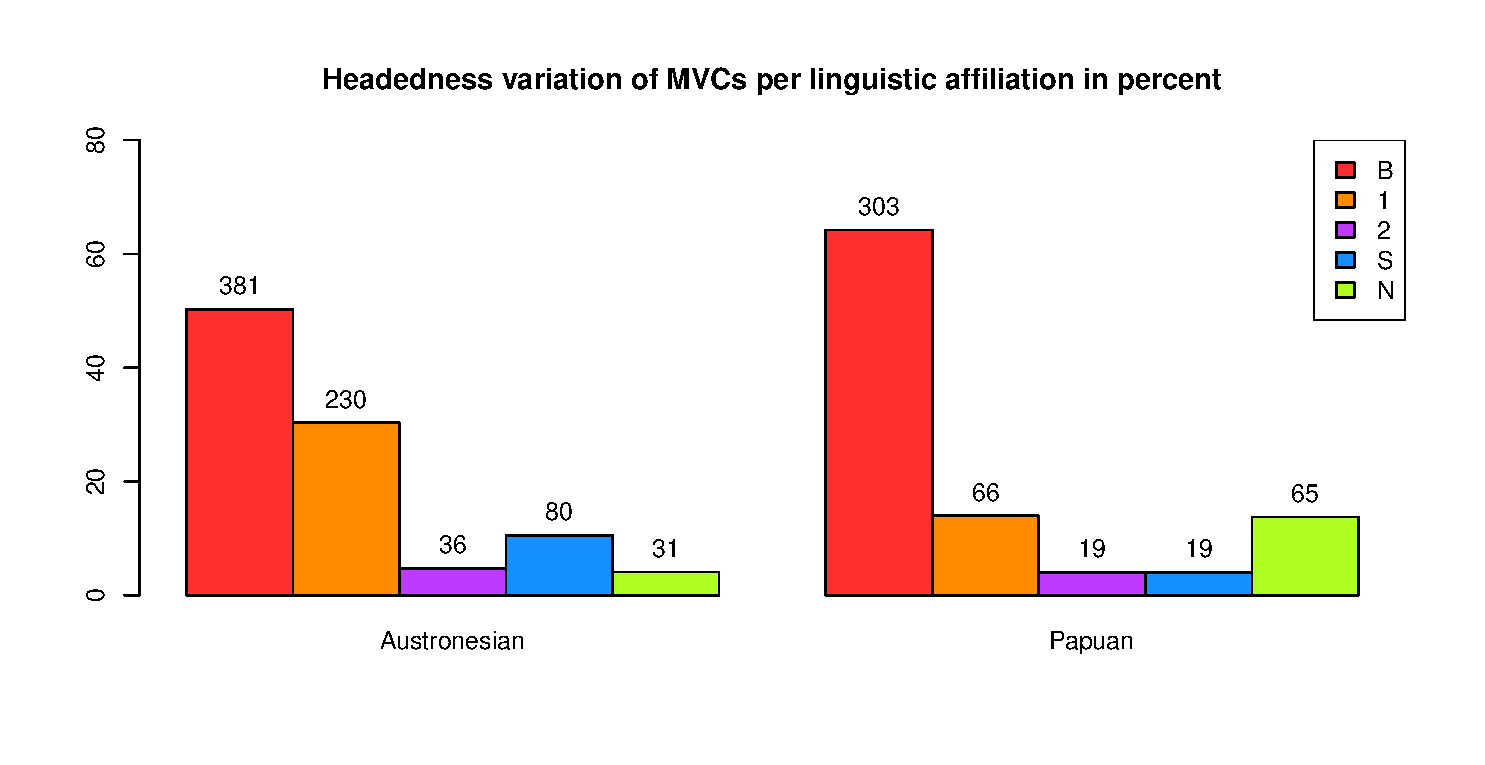
\includegraphics[width=\columnwidth]{figures/Headedness_Family.eps}
\caption[Headedness of MVCs per linguistic affiliation]{Headedness of MVCs per linguistic affiliation. B = Both verbs marked, 1 = First verb marked, 2 = Second/final verb marked, S = Shared affix set, N = None of the verbs marked. Numbers on top of the bars refer to the number of observations in the sample.}\label{fig:head-family}
\end{figure}
\begin{figure}[t]
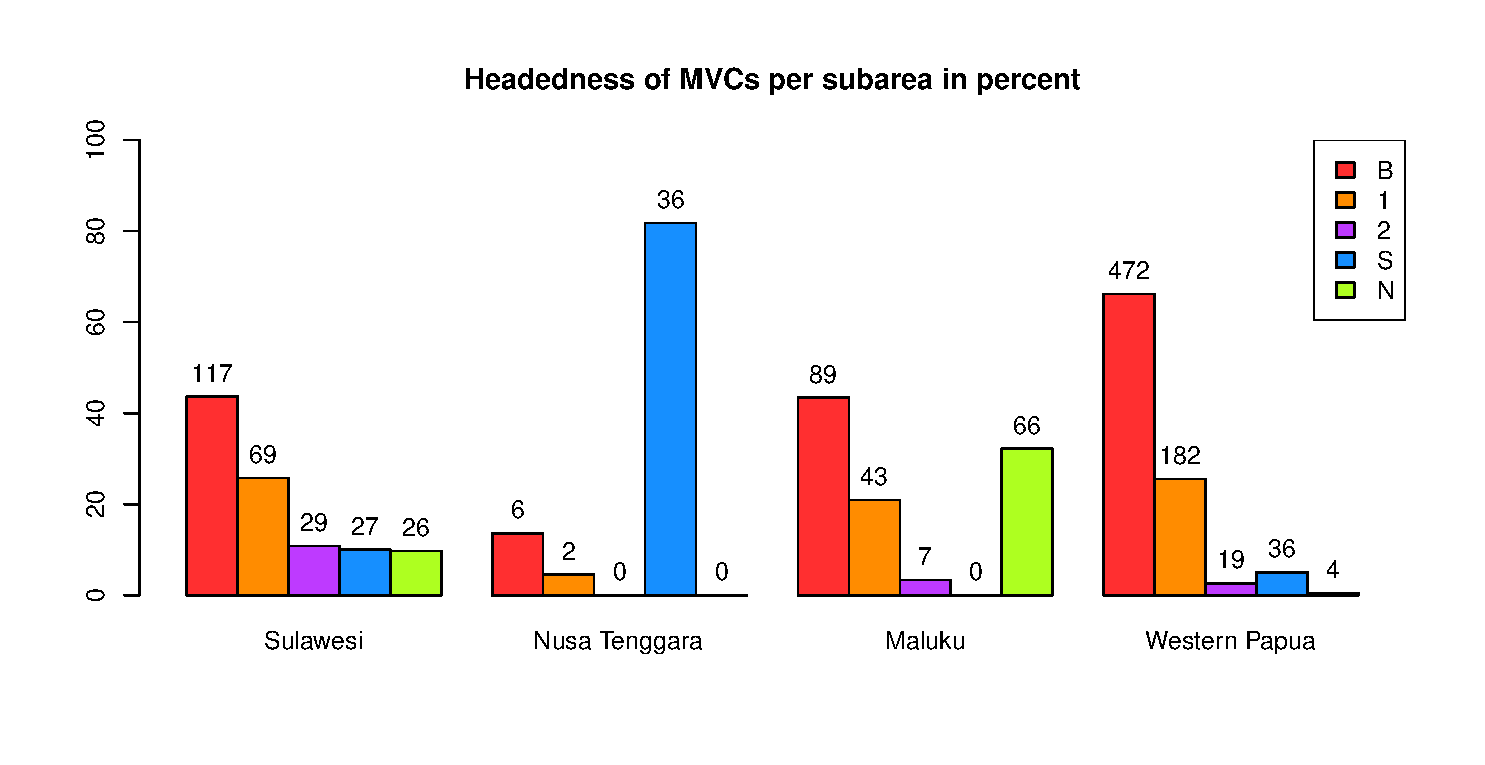
\includegraphics[width=\columnwidth]{figures/Headedness_Group.eps}
\caption[Headedness of MVCs per subarea]{Headedness of MVCs per subarea. B = Both verbs marked, 1 = First verb marked, 2 = Second/final verb marked, S = Shared affix set, N = None of the verbs marked. Numbers on top of the bars refer to the number of observations in the sample.}\label{fig:head-group}
\end{figure}

Rather surprisingly, a look at the choice of inflection patterns per language (\tabref{table:Headedness_per_lang}) clearly shows that only one language (\ili{Moskona}, \textsc{pap}) sticks to a single headedness pattern for all MVCs. All other languages use more than one option (though \ili{Tobelo} is another candidate for using a single pattern with only one outlier). The corpus language \ili{Wooi} illustrates the full range of variation, running the whole gamut of inflectional patterns from ``B" to ``N". As with most other languages in the sample, ``B" and ``1" constitute the dominant headedness patterns in \ili{Wooi}. The ``S" pattern is restricted to the cases of \ili{Wooi} modifier verbs, as already introduced in \sectref{sec:identifyingverbs}). The numbers for ``2" and ``N" only reflect irregular inflectional behaviour of loan verbs from the dominant national language, \ili{Indonesian}, as well as the item \textit{kay} `finish', a verboid lexeme that has undergone grammaticalisation towards a completive marker and thereby lost part of its inflectional ability. Example (\ref{wooi_andawa}) below is a combination of both an \ili{Indonesian} loan verb and \textit{kay}. Such instances were counted as ``N" since no inflection could be found (nor added, for that matter).\footnote{To be precise, the verbaliser \textit{ve-} does occasionally take a prefix to mark plural subjects, but has lost the ability to inflect for singular subject referents.}

\ea \label{wooi_andawa}
\langinfo{Wooi}{Austronesian, xSHWNG}{ikan\_ANDAWA\_ANTANAY}\\
\glll mara i vo vetau kay \\
mara i vo ve-tau kay \\
\textsc{top} \textsc{3}\textsc{sg} \textsc{top} \textsc{vblz}-know complete \\
\glft `As for him, he knows all (the story).' \\ 
\z

\newpage
What is notable from \tabref{table:Headedness_per_lang} below is that there are two kinds of distributional patterns. First, there is an overall trend towards ``B" followed by ``1" (yet not in all languages). Second, there are micro trends that only take place in single languages or small clusters of neighbouring languages. For instance, all instances of ``S" marking in the Sulawesi group are due to only \ili{Tolaki} and \ili{Tukang Besi}, both located in the far south-east of the island. The languages from central/northern Sulawesi, \ili{Pendau} and \ili{Tajio}, do not seem to make use of that pattern. 

\begin{table}
\begin{tabular}{lrrrrr}
  \lsptoprule
 & \multicolumn{1}{c}{B} & \multicolumn{1}{c}{1} & \multicolumn{1}{c}{2} & \multicolumn{1}{c}{S} & \multicolumn{1}{c}{N} \tabularnewline 
  \midrule
  \ili{Muna} &  46 &   0 &   4 &   0 &   0 \tabularnewline 
  \ili{Pendau} &  15 &  22 &  11 &   0 &   3 \tabularnewline 
  \ili{Tajio} &  18 &   4 &  10 &   0 &   0 \tabularnewline 
  \ili{Tolaki} &   0 &  37 &   0 &   5 &  23 \tabularnewline 
  \ili{Tukang Besi} &  38 &   6 &   4 &  22 &   0 \tabularnewline \midrule
  {\color{gray}Abui} & {\color{gray}\textit{NA}} & {\color{gray}\textit{NA}} & {\color{gray}\textit{NA}} &   {\color{gray}\textit{NA}} & {\color{gray}\textit{NA}} \tabularnewline 
  {\color{gray}Alorese} & {\color{gray}\textit{NA}} & {\color{gray}\textit{NA}} & {\color{gray}\textit{NA}} &   {\color{gray}\textit{NA}} & {\color{gray}\textit{NA}} \tabularnewline 
  {\color{gray}Bunaq} & {\color{gray}\textit{NA}} & {\color{gray}\textit{NA}} & {\color{gray}\textit{NA}} &   {\color{gray}\textit{NA}} & {\color{gray}\textit{NA}} \tabularnewline 
  {\color{gray}Kaera} & {\color{gray}\textit{NA}} & {\color{gray}\textit{NA}} & {\color{gray}\textit{NA}} &   {\color{gray}\textit{NA}} & {\color{gray}\textit{NA}} \tabularnewline
  \ili{Kambera} &  6 &   2 &   0 &  36 &   0 \tabularnewline
  {\color{gray}Klon} & {\color{gray}\textit{NA}} & {\color{gray}\textit{NA}} & {\color{gray}\textit{NA}} &   {\color{gray}\textit{NA}} & {\color{gray}\textit{NA}} \tabularnewline 
  {\color{gray}Makalero} & {\color{gray}\textit{NA}} & {\color{gray}\textit{NA}} & {\color{gray}\textit{NA}} &  {\color{gray}\textit{NA}} & {\color{gray}\textit{NA}} \tabularnewline 
  {\color{gray}Teiwa} & {\color{gray}\textit{NA}} & {\color{gray}\textit{NA}} & {\color{gray}\textit{NA}} &   {\color{gray}\textit{NA}} & {\color{gray}\textit{NA}} \tabularnewline 
  {\color{gray}Tetun} & {\color{gray}\textit{NA}} & {\color{gray}\textit{NA}} & {\color{gray}\textit{NA}} &   {\color{gray}\textit{NA}} & {\color{gray}\textit{NA}} \tabularnewline 
  {\color{gray}Waimaqa} & {\color{gray}\textit{NA}} & {\color{gray}\textit{NA}} & {\color{gray}\textit{NA}} &   {\color{gray}\textit{NA}} & {\color{gray}\textit{NA}} \tabularnewline 
  {\color{gray}Western Pantar} & {\color{gray}\textit{NA}} & {\color{gray}\textit{NA}} & {\color{gray}\textit{NA}} &  {\color{gray}\textit{NA}} & {\color{gray}\textit{NA}} \tabularnewline \midrule 
  {\color{gray}Buru} & {\color{gray}\textit{NA}} & {\color{gray}\textit{NA}} & {\color{gray}\textit{NA}} & {\color{gray}\textit{NA}} & {\color{gray}\textit{NA}} \tabularnewline
  \ili{Selaru} &  16 &   7 &   2 &   0 &   0 \tabularnewline 
  \ili{Taba} &  24 &  18 &   1 &   0 &   1 \tabularnewline 
  \ili{Tidore} & 6 & 18 & 3 & 0 & 65 \tabularnewline
  \ili{Tobelo} &  64 &   0 &   1 &   0 &   0 \tabularnewline \midrule 
  {\color{gray}Abun} & {\color{gray}\textit{NA}} & {\color{gray}\textit{NA}} & {\color{gray}\textit{NA}} &   {\color{gray}\textit{NA}} & {\color{gray}\textit{NA}} \tabularnewline
  \ili{Biak} &  59 &  34 &   0 &   1 &   0 \tabularnewline
  \ili{Dusner} &  36 &  22 &   0 &   0 &   0 \tabularnewline
  \ili{Hatam} &  47 &  29 &   0 &   0 &   0 \tabularnewline
  \ili{Inanwatan} &  18 &   4 &  14 &   6 &   0 \tabularnewline
  \ili{Maybrat} &  95 &   6 &   1 &   0 &   0 \tabularnewline 
  \ili{Mor} &  78 &  10 &   0 &   0 &   0 \tabularnewline
  \ili{Moskona} &  84 &   0 &   0 &   0 &   0 \tabularnewline
  \ili{Mpur} &  74 &   7 &   1 &   1 &   0 \tabularnewline
  \ili{Sougb} &  28 &   6 &   0 &   9 &   0 \tabularnewline 
  \ili{Wooi} & 115 &  70 &   3 &  16 &   3 \tabularnewline
   \lspbottomrule
\end{tabular}
\caption[Headedness variation per language]{Headedness variation per language. B = Both verbs marked, 1 = First verb marked, 2 = Second/final verb marked, S = Shared affix set, N = None of the verbs marked. Languages in grey, only displaying \textsc{NA} values, have been excluded from the calculation for reasons discussed in \sectref{sec:unreliable}}
\label{table:Headedness_per_lang}
\end{table}

In the following sections, I will provide some more examples for the different inflection patterns, and try to explain the most conspicuous numbers from \tabref{table:Headedness_per_lang}. To this end, I will subsume under the label ``symmetrical-head constructions" both the ``B" and the ``N" types. ``Asymmetrical-head constructions" refer to the patterns ``1" and ``2". Finally, ``distributed-head constructions" comprise the ``S" pattern.

\subsubsection{Symmetrical-head constructions}\label{sec:symmetrical-head}

Symmetrical-head constructions mark both/all verbs in exactly the same way, that is, either they are fully inflected, or no inflection whatsoever occurs on the verbs. The latter type is of course prevalent in isolating languages of the \textsc{nus} subarea as well as in \ili{Buru}, but these have been excluded for the reasons already discussed. If one just regards the languages that in principle have the grammatical means to construe asymmetrical headedness patterns, ``N" inflectional behaviour is virtually absent from all subareas, with two major exceptions. In the \textsc{mal} group, ``N" is the unmarked choice (in both senses of the term) to express MVCs in \ili{Tidore}. In Sulawesi, \ili{Tolaki} differs strongly from the other languages in the extent to which uninflected MVCs are in use. To illustrate this, let us have a closer look at \ili{Tolaki} ``N" inflection.

\citet{mead2008verb} refer to MVCs that only have the first verb inflected as dependent serialisation, and they offer plenty of examples from \ili{Tolaki}. In many of their examples, however, the first verb in sequence is not a semantically full-fledged verb that would add to the event frame of the construction, but rather a verboid with a grammatical rather than a semantic function. Therefore, when analysing such strings as a matrix construction featuring a grammaticalised verb on the one hand and a nested construction on the other, the nested construction would end up being annotated as ``N" since inflection is only attached to the matrix level verb. Here are two examples, each with a nested motion construction.

\ea \label{tolaki001}
\langinfo{Tolaki}{Austronesian, WMP}{\citealt[116]{mead2008verb}}\\
\gll lako-no-to lumaa lako um-ale-'iro banggona-no \\
go-3\textsc{sg}.\textsc{gen}-\textsc{perf} fly go $<$\textsc{m}$>$-take-3\textsc{pl}.\textsc{abs} companion-3\textsc{sg}.\textsc{gen} \\
\glft `Then he flew off and fetched his companions.' \\ 
\z

\ea \label{tolaki002}
\langinfo{Tolaki}{Austronesian, WMP}{\citealt[116]{mead2008verb}}\\
\gll a-no amba Anawaingguluri ina'u me-titiro i pu'u nohu \\
and-3\textsc{sg}.\textsc{nom} then Anawaingguluri descend $<$\textsc{m}$>$:\textsc{intr}-look-.down at base mortar \\
\glft `At that point Anawaingguluri went down and peered down at the base of the mortar.'\\ 
\z

In both (\ref{tolaki001}) and (\ref{tolaki002}) only the first verboid takes subject inflection\footnote{Note that the indexer may act as an enclitic and is then attracted to clause-initial ``single syllable relators" \citep[114]{mead2008verb}, as in (\ref{tolaki002}) where \textit{-no} is attracted to the left and the verboid \textit{amba} remains bare.}, \textit{lako} `go' (translated as `then') and \textit{amba} `then', both conveying some sequentialising function within the discourse context (next, X happened, where X is filled by a nested MVC). According to my understanding, cases like (\ref{tolaki001}) are hierarchically structured with one or more nested constructions inside (\textsc{stacked MVCs}, see also \sectref{sec:stackedmvcs}). Here, \textit{lumaa}, the second \textit{lako} and \textit{ale} together form a subordinate motion-to-action MVC which in turn has an embedded motion complex in slot 1, consisting of \textit{lumaa} and \textit{lako} (`fly go' meaning `flying off/away from situational centre'). \figref{figure:tolakiMVC} illustrates what I take to be the internal make-up of example (\ref{tolaki001}).

\begin{figure}[h]
\jtree[xunit=8em,yunit=1em]
\! = {\textit{lako lumaa lako ale}}{sequentialising}
: {\textit{lako}} {\textit{lumaa lako ale}}{motion-to-action}
: ({\textit{lumaa lako}}{motion complex}) {\textit{ale}}.
\endjtree
\caption[Internal structure of example (\ref{tolaki001}) from \ili{Tolaki}]{Internal structure of example (\ref{tolaki001}) from \ili{Tolaki}. Terms underneath the verbs name the respective construction.}
\label{figure:tolakiMVC}
\end{figure}

Each MVC receives its own encoding in the EI sample, and as only the topmost verb, \textit{lako}, is inflected for person, I annotated the two nested MVCs as ``N". It is this procedure that accounts for the surprising number of 23 uninflected \ili{Tolaki} MVCs. Example (\ref{tolaki002}) has a similar internal structure with \textit{ina'u} `descend' and \textit{me-titiro} `look-down' forming another motion-to-action MVC.

Turning to the second type of symmetrical-head constructions, we see that in all three subareas \textsc{sul}, \textsc{mal} and \textsc{pap}, the ``B" pattern clearly dominates, with the mentioned exceptions. The following examples illustrate different inflectional categories from the subareas. In Sulawesi, mood and voice are marked on the verbs in the north, while person indexers appear on the verbs from the south-eastern languages. In \ili{Muna} the mood system is integrated into the subject indexer morphology in the sense that there are two sets of indexers, one indicating realis, and another one indicating irrealis. In both Sulawesi examples below, there has to be agreement between the grammatical categories marked on the verbs: the mood values in \ili{Pendau}, and the mood values as well as the person indexers in \ili{Muna}. Recall that in \ili{Pendau} there is a subset of motion verbs that fail to inflect, causing many motion MVCs to be either ``1" or ``2".

\ea 
\langinfo{Pendau}{Austronesian, WMP}{\citealt[355]{Quick2007}}\\
\glll a'u menyau mobanta ridagat \\
a'u \textsc{m}-pe-nyau \textsc{m}-po$_1$-banta ri=dagat \\
1\textsc{sg}.\textsc{abs} \textsc{irr}-\textsc{sf}-go.down \textsc{irr}-\textsc{sf}-fish \textsc{loc}=ocean \\
\glft `I will go down to fish in the ocean.'\\ 
\z

\ea 
\langinfo{Muna}{Austronesian, WMP}{\citealt[236]{vandenberg1989}}\\
\gll naewine da-si-kala-ha dae-kabua we tehi \\
tomorrow 1\textsc{pl}.\textsc{irr}-\textsc{si}-go-\textsc{ha} 1\textsc{pl}.\textsc{irr}-fish \textsc{loc} sea \\
\glft `Tomorrow we will go fishing together in the sea.' \\ 
\z

\ili{Selaru}, \ili{Taba} and \ili{Tobelo} from Maluku are very similar in that they all mark subjects (in \ili{Tobelo} also objects) on the verbs, and the majority of their MVCs are symmetrically inflected, with all verbs attracting inflection. Example (\ref{sel1}) from \ili{Selaru} illustrates this pattern. The matrix construction is a delimitative coordination explicitly marked by use of \textit{ma}.\footnote{\textit{Ma} clearly belongs to the complex of \textsc{come} verbs that are almost ubiquitous in the EI area. Other languages like \ili{Wooi} still employ cognates of this lexeme as verbs or directionals, and the verbal character is still more or less visible. Since Coward glosses \textit{ma} as a conjunction, and explicitly refers to it as a conjunctive marker, I have refrained from treating it as a verb in \ili{Selaru}.} Delimitative constructions consist of both a main event and a delimiting event (x takes place \textit{until} y happens), and are mostly construed as plain biclausal constructions in EI. In this example, the first clause consists of a two-verb cause-result MVC, and both verbs, \textit{sil} `beat' and \textit{hunw} `murder', receive full person indexing inflection.

\ea \label{sel1}
\langinfo{Selaru}{Austronesian, CMP}{\citealt[125]{coward2005}}\\
\gll mw-sil-a mw-hunw-a i ma y-maty \\
2\textsc{sg}-beat-Ø 2\textsc{sg}-murder-Ø him \textsc{conj} 3\textsc{sg}-die \\
\glft `... you beat and murdered him until he died.'\\ 
\z

Symmetrical head marking is also the most common choice in the languages from Western Papua, with the exception of isolating \ili{Abun}. The most consistent language in this group is \ili{Moskona} with all 84 instances of MVCs in the sample being construed as ``B". \ili{Moskona} is a typical West Papuan language with subject agreement prefixes on the verb and moderate verb morphology. Person marking on the verb is consistently carried out whereby third person singular subjects are zero-marked. The following two examples show position-action MVCs that have been grammaticalised to a certain extent to mark aspectual information (continuous or progressive aspect; \citealt[296]{gravelle2010grammar}). The singular example looks just like an unmarked ``N" MVC. Yet, within the \ili{Moskona} subject marking paradigm, it is clear that the very same construction would receive person marking with any other person/number constellation, and so has been annotated ``B" as well.

\ea 
\langinfo{Moskona}{Papuan, EBH}{\citealt[296]{gravelle2010grammar}}\\
\gll Petrus ah omk(a) jig jog. \\
Petrus lie sleep.deep \textsc{loc} already \\
\glft `Petrus was already sleeping deeply.’ \\ 
\z

\ea 
\langinfo{Moskona}{Papuan, EBH}{\citealt[296]{gravelle2010grammar}}\\
\gll Eri i-ot i-eregejg(a) ofa. \\
they.\textsc{pl} 3\textsc{pl}-stand 3\textsc{pl}-surround s/he \\
\glft `They were (standing) around him.’\\ 
\z

\subsubsection{Asymmetrical-head constructions} \label{sec:asymmetrical}

Asymmetrical-head constructions assign verbal inflection to one of the verbs only, leaving the other(s) without prefixes or suffixes. The inflected verb may either stand in V$_1$ position (the ``1" type) or in construction-final position (``2"). If the head of a MVC is expected to go where the main verb goes in simplex clauses then one might expect that in asymmetrical-head constructions Papuan-style AOV languages would have the last verb of a MVC marked as head (see also \citealt{Durie1997} on this point). This is, however, not a consistent trend in the dataset. There are a total of nine (Papuan) languages in the sample with AOV word order of which only one language, \ili{Inanwatan} from the Papua group, shows a preponderance of ``2" MVCs. All other languages are either not equipped with reliable verbal morphology (Nusa Tenggara) or do not show any inclination towards asymmetrical-head constructions at all (\ili{Tobelo} from the Maluku group). As only \ili{Inanwatan} behaves fully ``Papuan" in this respect, we cannot, at this point, confirm such a hypothesis. Before I take a closer look at the \ili{Inanwatan} MVC system, however, I would like to make mention of one other language in the sample that seems to behave in a ``Papuan" way in terms of head-final marking.

In \ili{Abui} (\textsc{nus} group), as mentioned before, there are two inflectional categories realised on the verbs. First, there is the by-now-familiar unreliable person indexing morpholgy, basically indicating undergoer arguments but at times also S. And second, there is an aspectual category with verbal suffixes denoting perfective, imperfective and durative temporal frames. It is these suffixes that seem to indicate that the last verb in a MVC could indeed be interpreted as a Papuan final verb, or at any rate as the head of the construction. When there is an aspectual suffix, it always seems to go with the last verb \citep[350]{kratochvil2007grammar}. However, as these aspectuals are not obligatory, and do not appear with every MVC, I did not count those instances as inflection. It might very well be the case that aspectual behaviour is a better indicator of headedness in \ili{Abui} MVCs than unreliable person indexing.  

\largerpage[1]
\ili{Inanwatan} appears to be the only language in the sample that consistently makes use of the ``2" pattern in certain MVCs. The structure is bare verb - subject indexer - second verb - tense suffix. De Vries refers to those constructions as complex phrasal verbs \citep[57]{devries2004}. The second verb slot involves most often a (directed) motion verb, but other combinations are found as well. Examples (\ref{inan1}) to (\ref{inan3}) illustrate the pattern. Recall from \sectref{sec:westpapua2} that verb inflection in \ili{Inanwatan} is marked both by prefix sets for subject and objects (indicating person and number), as well as by suffixes denoting tense and gender in third person singular forms of the subject argument. Therefore \textit{noé} `go.out' in example (\ref{inan1}), for instance, clearly stands out as a preposed bare verb stem.

\ea \label{inan1}
\langinfo{Inanwatan}{Papuan, SBH}{\citealt[48f.]{devries2004}}\\
\gll mé-se-i mé-se-i mé-se-i ewáiwa, nóe-we-i-di \\
3\textsc{sbj}-walk-\textsc{pst}.\textsc{m} 3\textsc{sbj}-walk-\textsc{pst}.\textsc{m} 3\textsc{sbj}-walk-\textsc{pst}.\textsc{m} and go.out-3\textsc{sbj}-descend-\textsc{pst}.\textsc{m} \\
\glft `He went on and on and on and he arrived.' \\ 
\z

\ea \label{inan2}
\langinfo{Inanwatan}{Papuan, SBH}{\citealt[47]{devries2004}}\\
\gll gáago-wo dópis ewái ísi-we-ge-rita-re obapasa ewái \\
side-at chamber this.\textsc{f} fill-3\textsc{sbj}-do-\textsc{hab}-\textsc{pst} gunpowder this.\textsc{f} \\
\glft `At the side they used to fill the chamber with gunpowder.'\\ 
\z

\ea \label{inan3}
\langinfo{Inanwatan}{Papuan, SBH}{\citealt[44]{devries2004}}\\
\gll tíra-tira-we-i-rita-re ewáiwa íde-wó-u-rita-re \\
take-take-3\textsc{sbj}-pierce-\textsc{hab}-\textsc{pst} and \textsc{intr}-3\textsc{sbj}-fell-\textsc{hab}-\textsc{pst} \\
\glft `They pierced it repeatedly and then it would fall.'\\ 
\z

The examples show the three main functions of the \ili{Inanwatan} ``2" pattern. In (\ref{inan1}) a motion verb is combined with another motion verb to form a complex motion event. The first slot may feature different motion verbs, such as \textit{mo} `come', \textit{mogo} `carry' or \textit{qai} `follow', while the second slot hosts directed motion verbs specifying the path of the motion event. The next example in (\ref{inan2}) is a loanverb carrier construction in which the loanword comes first as a bare verb stem (\textit{isi} is a loan from \ili{Indonesian} \textit{(meng)isi}, `fill (into)') followed by an inflected \textsc{do} verb. This is functionally equivalent to a widespread verbaliser construction in West Papuan languages involving a form \textit{ve/be} (for instance, in \ili{Wooi} and \ili{Biak}). The third example in (\ref{inan3}) shows another use of the pattern. Here a \textsc{take} verb in V$_1$ is combined with some other action verb in V$_2$. \textit{Tira} may have already lost part of its lexical semantics in this construction, and could possibly express some kind of direct or total effectedness of the patient of \textit{i} `pierce'. In \ili{Tetun Fehan}, for instance, the \textsc{take} -- action construction grammaticalises into a marker of successful action. In (\ref{inan3}), however, we can still recognise a typical cause-result structure `take something (and) pierce it (immediately)'. Note that the reduplication pattern suggests that both verbs indeed form a tight semantic unit: although it is the first verb \textit{tira} that is reduplicated, it seems clear from the given translation that it is an action of repeated piercing, not of repeated taking followed by a single piercing action.

\subsubsection{Distributed-head constructions}

Distributed-head constructions share a set of affixes, and both verbs seem to receive the same constituent status. Alternatively, one could analyse both verbs as forming one phrasal head instead of a lexical head. This head marking pattern is quite closely related to van Staden and Reesink's concept of complex serialisation in that both verbs form what is perceived to be an inseparable unit. Unlike Van Staden and Reesink, however, I also included cases in which both verbs appear within one phonological word (that is, having just one main accent). Distributed-head constructions are quite rare in the sample. They seem to be absent from the Moluccan languages, and appear only in a very small subset of languages in the other three subareas. In the \textsc{sul} group, the ``S" pattern is confined to south-eastern \ili{Tolaki} and \ili{Tukang Besi} (but not \ili{Muna}). The pattern then reappears prominently in \ili{Kambera}, and is used consistently in \ili{Inanwatan}, \ili{Sougb}, and \ili{Wooi}.

Detecting distributed-head constructions is less straightforward than detecting other inflectional patterns. This is because the pattern stands out clearly only if a given language employs both prefixes and suffixes. This is the case in \ili{Tukang Besi}, \ili{Kambera}, and \ili{Wooi}, but not in \ili{Tolaki} and \ili{Sougb}. My analysis of these languages should therefore be treated with some caution. Turning to the unambiguous cases first, the following examples provide illustrations of "S"-inflected MVCs in \ili{Tukang Besi} and \ili{Kambera}. \ili{Tukang Besi} ``S" MVCs are headed by a subject indexer in the prefix slot and may have an object pronominal form at the end of the complex. Object agreement in \ili{Tukang Besi} changes the argument alignment in that a full object NP must be marked with the nominative case instead of using the non-nominative core-article \textit{te}. The use of object indexers ``implies perfectivity, greater individuation of the object, and more total affectedness of the object" \citep[135]{donohue1999}. It is thus not directly connected to a certain type of MVC encoding but is instead sensitive to expressing grammatical or discourse notions.

\ea \label{tukang001}
\langinfo{Tukang Besi}{Austronesian, WMP}{\citealt[182]{donohue1999}}\\
\ea
\gll no-helo'a te roukau ako te ana-no \\
3\textsc{rls}-cook \textsc{core} vegetables do.for \textsc{core} child-3\textsc{poss} \\
\glft `She cooked the vegetables for her children.' \\ 
\ex \label{tukang001b}
\gll no-helo'a-ako te ana-no te roukau \\ 
3\textsc{rls}-cook-do.for \textsc{core} child-3\textsc{poss} \textsc{core} vegetables \\
\glft `She cooked the vegetables for her children.' \\ 
\z
\z

\ea \label{tukang002}
\langinfo{Tukang Besi}{Austronesian, WMP}{\citealt[183]{donohue1999}}\\
\gll no-tutu-molobu-'e na kabali te La Mbagi \\
3\textsc{rls}-pound-straight-3\textsc{obj} \textsc{nom} machete \textsc{core} La Mbagi \\
\glft `La Mbagi beat the machete blade straight.' \\ 
\z

The first example pair (\ref{tukang001}) shows a non-contiguous construal with the two verbs, \textit{helo'a} and \textit{ako}, being placed in separate VPs, and a contiguous construal with both verbs appearing within what seems to be one phonological unit. As no clear semantic difference is given, it seems that both constructions convey more or less the same meaning (this seems rather exceptional among EI MVCs). The undergoer arguments in both constructions are marked with the \textsc{core} marker \textit{te}. \footnote{Note that each of the verbs assigns a \textsc{core} case role to a referent. As these referents, the O and the G argument, are not co-referential one might wonder if this does not instead suggest a biclausal construal. Example (\ref{tukang001b}) therefore seems to combine contradictory signals: while the full phonological integration of both verbs appears to mirror a tight syntactic unit, the case assignment to the arguments suggests two independent argument sets, and thus a biclausal construal rather than a monoclausal one.} The last example in (\ref{tukang002}) illustrates another way of construing a clear ``S" inflectional pattern in \ili{Tukang Besi}. This type is found with unaccusative verbs in V$_2$ position, and involves a switch-function interpretation (the O argument of V$_1$ becomes the S argument of V$_2$). Note that the use of the object suffix results in a switch in case-marking: the A argument is now marked with the \textsc{core} marker \textit{te} and the O argument receives nominative marking.

\largerpage[1]
The \ili{Kambera} ``S" pattern is quite similar to the \ili{Tukang Besi} pattern. The (two) verbs are placed in clause-initial position framed by one or more person indexer(s) in prefix and/or suffix position, and aspectual suffixes. The following examples illustrate typical cases. In (\ref{kambera001}) two motion verbs are combined to form a motion complex. In this construction, the first verb seems to have lost its andative path semantics and V$_2$ \textit{mai} contributes a path specification instead. This kind of motion combination is also found in other languages of the area (for instance, in \ili{Wooi}). The ``S" inflectional pattern is clearly marked off with the nominative marker in front and the imperfective clitic \textit{-pa}. Prefix indexers can, however, also be absent, as in the following example (\ref{kambera002}). Here, the first verb of the MVC, \textit{taka} `arrive', does not literally evoke a spatial dislocation of the subject but rather performs a sequentialising function. As the nominative marker is not repeated, there is no prefix indicating the ``S" pattern. Yet my interpretation here is that as long as a prefix is licit, cases like this one should also be included in the ``S" group. In other words, if there is a slot for a given affix, and there are contexts in which the use of the affix is prevented, the whole construction nonetheless conforms to the ``S" pattern.

\ea \label{kambera001}
\langinfo{Kambera}{Austronesian, CMP}{\citealt[339]{klamer1998grammar}}\\
\gll na-laku mái-pa pa-hili karai-ka \\
3\textsc{sg}.\textsc{nom}-go come-\textsc{ipfv} \textsc{ctr}-again ask-1\textsc{sg}.\textsc{acc} \\
\glft `He came yet again to ask me again.'\\ 
\z

\ea \label{kambera002}
\langinfo{Kambera}{Austronesian, CMP}{\citealt[357]{klamer1998grammar}}\\
\gll ba reu-reu padua-na-ka dá, tàka njàrung-na-nya-ka dumu \\
\textsc{conj} \textsc{rdp}-talk in\_the\_middle-3\textsc{sg}.\textsc{gen}-\textsc{perf} inside arrive punch-3\textsc{sg}.\textsc{gen}-3\textsc{sg}.\textsc{dat}-\textsc{perf} \textsc{emph}.2\textsc{sg} \\
\glft `(And) he (=J) was inside in the middle of talking, then he (=older brother) punched him (=J) ...'\\ 
\z

\subsection{Contiguity}\label{sec:contiguity}

Contiguity refers to the distribution of verbal constituents within a given MVC, and is applied here as a measure of distance between the verbs. Contiguous verbs in a MVC are directly adjacent to each other, only allowing for verbal morphology to intervene within their sequence. If both verbs form part of one phonological word, as for instance in \ili{Inanwatan}, the MVC is coded as ``W". The most common case, however, is the ``C" pattern (contiguous yet being part of different phonological words). As \tabref{table:Contiguity_overview} shows, adjacent verbs that are phonologically independent form the most common contiguity pattern found in the EI languages, with a total of 1584 cases. Both macro affiliations, Austronesian and Papuan, overall favour the ``C" pattern over all other contiguity configurations (see also \figref{fig:adj-family} below). The other option for contiguous MVCs, the within-word pattern ``W", is only found in a few languages, mostly in the Papua group. With most languages, the ``W" pattern seems to only show up accidentally or in specific low-frequency constructions. So, for instance in \ili{Wooi}, there is only erratic or obsolete use of within-word MVCs (for examples and discussion, see next section).

\begin{table}
\begin{tabular}{lrrrrrr}
  \lsptoprule
 & \multicolumn{1}{c}{W} & \multicolumn{1}{c}{C} & \multicolumn{1}{c}{1} & \multicolumn{1}{c}{2} & \multicolumn{1}{c}{3} & \multicolumn{1}{c}{4} \tabularnewline 
  \midrule
   Austronesian &   11 & 873 & 205 &  25 &  7 & 1 \tabularnewline 
   Papuan &  34 & 711 & 248 &  29 & 2 & 0 \tabularnewline 
   \midrule
   Sulawesi &   0 & 218 &  45 &   4 &   0 &   1 \tabularnewline
   Nusa Tenggara &   0 & 670 & 156 &  26 &   7 &   0 \tabularnewline
   Maluku &   8 &  203 &  56 &  6 &   0 &   0 \tabularnewline 
   Western Papua &  37 & 493 & 196 &  18 &   2 &   0 \tabularnewline 
   \midrule
   Total & 45 & 1584 & 453 & 54 & 9 & 1 \tabularnewline
\lspbottomrule
\end{tabular}
\caption[Contiguity variation in the EI sample]{Overview of contiguity variation in the EI languages. W = Within word, C = Contiguous verbs 1 = One non-verbal constituent intervening, 2 = Two non-verbal constituents intervening, 3 = Three non-verbal constituents intervening, 4 = Four non-verbal constituents intervening. Note that both subcalculations, i.e., into language family affiliation as well as into areal subgroups, amount to the total number of observations given in the last row.}
\label{table:Contiguity_overview}
\end{table}

\largerpage[1]
When morphemic material intervenes between the verbal constituents, the first question is how to quantify the intervening elements. One could in principle either count morphemes, words, or constituents. I decided to adopt the last option as this would avoid biased counts of single constituents consisting of many morphemes or words. As displayed by the numbers, the EI languages frequently allowed one non-verbal constituent to appear between the verbs. Cases with more than one constituent were only rarely found, the most extreme being MVCs which seem to have their verbs separated by four constituents. Intervening constituents were in general more common in the Maluku and Papua group than in the other two groups: The ``1" pattern comprised about 30\% of the cases in  \textsc{mal} and \textsc{pap}, as opposed to just slightly below 20\% in \textsc{sul} and \textsc{nus}. \figref{fig:adj-group} shows the plots for degree of contiguity by subarea. No major deviation from the general pattern is to be seen, which again suggests that neither genetic affiliation nor subarea have any bearing on preferences in verb contiguity.

\begin{figure}
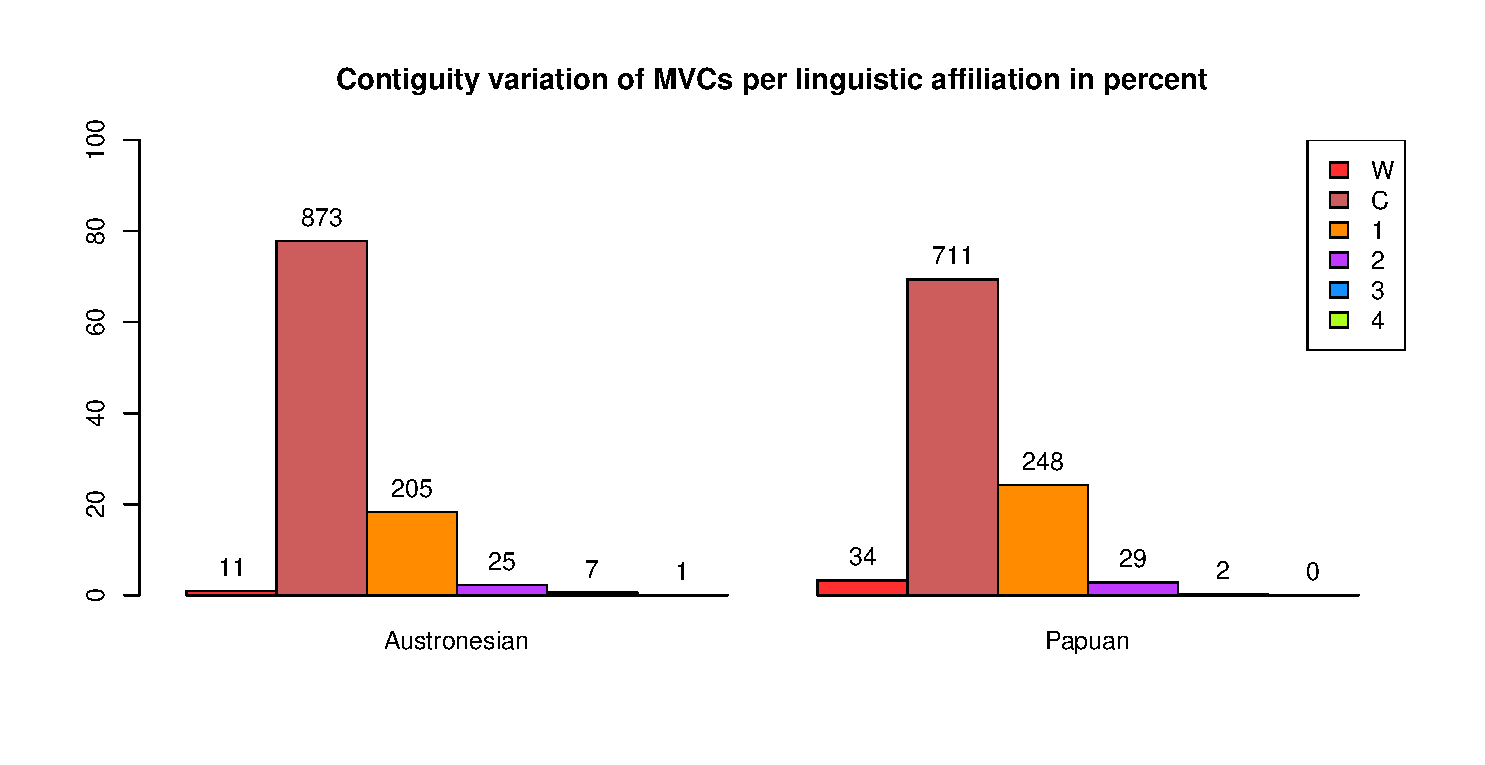
\includegraphics[width=\columnwidth]{figures/Contiguity_Family.eps}
\caption[Contiguity of MVCs by linguistic affiliation]{Contiguity of MVCs by linguistic affiliation in percent. W = Within word, C = Contiguous verbs 1 = One non-verbal constituent intervening, 2 = Two non-verbal constituents intervening, 3 = Three non-verbal constituents intervening, 4 = Four non-verbal constituents intervening. Numbers on top of the bars refer to the number of observations in the sample.}\label{fig:adj-family}
\end{figure}
\begin{figure}
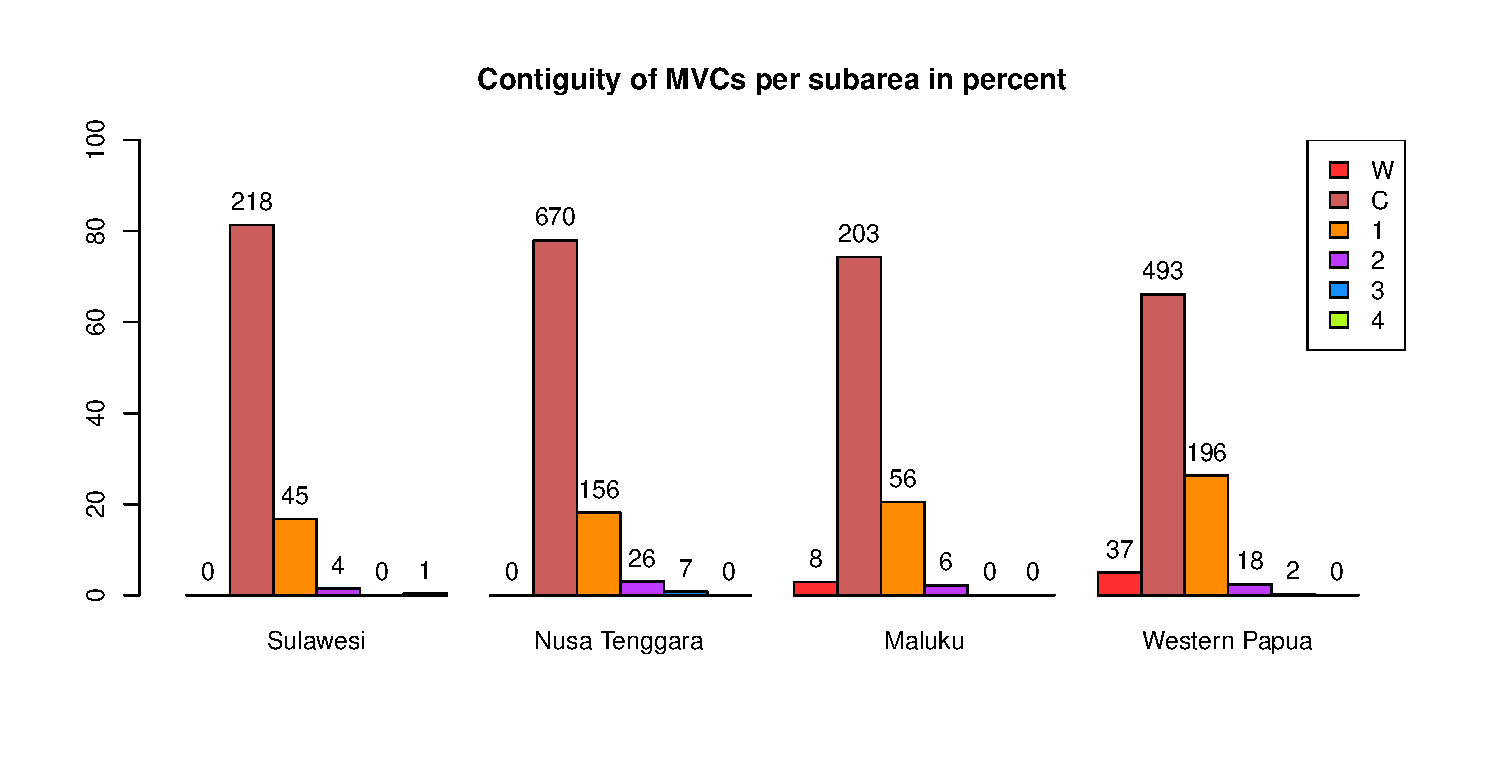
\includegraphics[width=\columnwidth]{figures/Contiguity_Group.eps}
\caption[Contiguity of MVCs by subarea]{Contiguity of MVCs by subarea in percent. W = Within word, C = Contiguous verbs 1 = One non-verbal constituent intervening, 2 = Two non-verbal constituents intervening, 3 = Three non-verbal constituents intervening, 4 = Four non-verbal constituents intervening. Numbers on top of the bars refer to the number of observations in the sample.}\label{fig:adj-group}
\end{figure}

\begin{table}
\begin{tabular}{lrrrrrr}
  \lsptoprule
 & \multicolumn{1}{c}{W} & \multicolumn{1}{c}{C} & \multicolumn{1}{c}{1} & \multicolumn{1}{c}{2} & \multicolumn{1}{c}{3} & \multicolumn{1}{c}{4} \tabularnewline 
  \midrule
  \ili{Muna} &   0 &  34 &  13 &   2 &   0 &   1 \tabularnewline 
  \ili{Pendau} &   0 &  45 &   6 &   0 &   0 &   0 \tabularnewline 
  \ili{Tajio} &   0 &  24 &   8 &   0 &   0 &   0 \tabularnewline 
  \ili{Tolaki} &   0 &  54 &  9 &   2 &   0 &   0 \tabularnewline 
  \ili{Tukang Besi} &   0 &  61 &   9 &   0 &   0 &   0 \tabularnewline \midrule
  \ili{Abui} &   0 &  93 &  15 &   1 &   0 &   0 \tabularnewline 
  \ili{Alorese} &   0 &  33 &  13 &   1 &   0 &   0 \tabularnewline 
  \ili{Bunaq} &   0 &  70 &  17 &   0 &   0 &   0 \tabularnewline 
  \ili{Kaera} &   0 &  13 &  9 &   2 &   0 &   0 \tabularnewline 
  \ili{Kambera} &   0 &  41 &   3 &   0 &   0 &   0 \tabularnewline 
  \ili{Klon} &   0 &  76 &  21 &   3 &   0 &   0 \tabularnewline 
  \ili{Makalero} &   0 &  67 &  8 &   1 &   0 &   0 \tabularnewline 
  \ili{Teiwa} &   0 &  63 &  19 &   2 &  1 &   0 \tabularnewline 
  Tetun &   0 &  57 &  16 &   0 &   0 &   0 \tabularnewline 
  Waimaqa &   0 & 126 &  29 &  15 &   6 &   0 \tabularnewline 
  Western Pantar &   0 &  31 &   6 &   1 &   0 &   0 \tabularnewline \midrule
  \ili{Buru} & 8 & 51 & 9 & 0 & 0 & 0 \tabularnewline
  \ili{Selaru} &   0 &  17 &  7 &  1 &   0 &   0 \tabularnewline 
  \ili{Taba} &   0 &  34 &  10 &   0 &   0 &   0 \tabularnewline 
  \ili{Tidore} & 0 & 66 & 22 & 4 & 0 & 0 \tabularnewline
  \ili{Tobelo} &   0 &  35 &  8 &   1 &   0 &   0 \tabularnewline 
\midrule
  \ili{Abun} &   0 &  19 &  14 &   0 &   0 &   0 \tabularnewline 
  \ili{Biak} &   0 &  51 &  15 &   1 &   0 &   0 \tabularnewline 
  \ili{Dusner} &   0 &  28 &  21 &   0 &   0 &   0 \tabularnewline 
  \ili{Hatam} &   0 &  25 &  22 &   2 &   0 &   0 \tabularnewline 
  \ili{Inanwatan} &  20 &  5 &   1 &   2 &   0 &   0 \tabularnewline
  \ili{Maybrat} &   0 &  55 &  23 &   0 &   0 &   0 \tabularnewline 
  \ili{Mor} &   0 &  62 &  6 &   2 &   1 &   0 \tabularnewline 
  \ili{Moskona} &   0 &  41 &  35 &   3 &   0 &   0 \tabularnewline 
  \ili{Mpur} &   1 &  39 &  19 &   3 &   0 &   0 \tabularnewline 
  \ili{Sougb} &  13 &   13 &  9 &   4 &   1 &   0 \tabularnewline 
  \ili{Wooi} &   3 & 155 &  31 &   1 &   0 &   0\tabularnewline 
   \lspbottomrule
\end{tabular}
\caption[Contiguity variation by language]{Contiguity variation by language. W = Within word, C = Contiguous verbs 1 = One non-verbal constituent intervening, 2 = Two non-verbal constituents intervening, 3 = Three non-verbal constituents intervening, 4 = Four non-verbal constituents intervening.}
\label{table:Contiguity_per_lang}
\end{table}

When we turn to contiguity variation by language (cf. \tabref{table:Contiguity_per_lang}) we see that the distribution is again quite even across the EI languages. What seems surprising is that there is not a single language that seems to use just one of the patterns for all its MVCs: All languages have MVCs with contiguous verbs, and others with non-contiguous verbs. Certain constructions may be predisposed towards specific contiguity patterns (e.g., motion constructions might tend towards ``C" because V$_1$ typically hosts an intransitive verb so that no direct object may go between it and the following verb). Alternatively, certain constructions/ languages may not impose specific restrictions, so that speakers are free to insert non-verbal constituents into any MVC (for instance, adverbials; as long as limits of information-load are not transgressed). 

\largerpage[1]
A closer inspection of the data seems to suggest that both cases in fact contribute to the general pattern. In some languages, certain constructions indeed remain stable, in that a constructional template seems to receive a fixed order of constituents. This is particularily clear in instances of MVCs within a single phonological unit. For instance, in \ili{Inanwatan}, motion complex constructions involving one motion event that is dissected into two or more verbal event descriptors consistently appear in ``W" construals, as illustrated in (\ref{inanwatan004}) below. The first verb, \textit{mogó} `carry', remains uninflected and attaches to the second verb or verbal complex (like \textit{de-wo} in the example), which is inflected for person and syntactic function (prefix), as well as for tense, number and gender (suffix).

\ea \label{inanwatan004}
\langinfo{Inanwatan}{Papuan, SBH}{\citealt[44]{devries2004}}\\
\gll mái-wo wó-uwu-i ewáiwa, ao nésar áwuga-era-era-ro tétewo mogó-we-de-wo-i \\
here-to 3\textsc{sbj}-sit-\textsc{pst}.\textsc{sg}.\textsc{m} and his smithy iron-piece-piece-\textsc{pl} all carry-3\textsc{sbj}-go.across-come-\textsc{pst}.\textsc{sg}.\textsc{m} \\
\glft `Here he settled, and he brought across pieces of iron for his smithy.'\\ 
\z

Verb contiguity is thus in many cases directly influenced by properties more general to the given language: as would be expected in verb-final languages like \ili{Inanwatan}, the object of the transport verb \textit{mogo} precedes the verbal complex. Similar constructions in verb-second languages confirm this: the object of the transport verb in V$_1$ appears postverbally and thus before V$_2$, typically leading to a ``1" pattern if the theme argument of the transport process is expressed. (\ref{pendau016}) is an example from \ili{Pendau}:

\ea  \label{pendau016}
\langinfo{Pendau}{Austronesian, WMP}{\citealt[345]{Quick2007}}\\
\glll io nongkomung tuainyo uo manyau rigii nudagat \\
io N-pong-'omung tuai=nyo 'uo ma-nyau ri=gii nu=dagat \\
3\textsc{sg}.\textsc{abs} \textsc{rls}-\textsc{sf}-carry y.sibling=3\textsc{sg}.\textsc{gen} yonder \textsc{ug}:\textsc{irr}-go.down \textsc{loc}=edge \textsc{cn}:\textsc{gen}=ocean \\
\glft `She carried her baby sister down to the edge of the ocean.'\\
\z

Certain constructions may on the other hand allow for variation with regard to interverbal constituents. Motion-to-action constructions in \ili{Waima'a}, for instance, are commonly construed with the ``C" pattern (as in (\ref{waimaqa003}) below). However, up to three constituents may occur between the verbs, as in example (\ref{waimaqa004}), where an adverbial (\textit{nan}), a goal NP (\textit{basara}) and a proform (\textit{wuo-ruo}) are placed before V$_2$ which saturates the action slot of the motion-to-action template.\footnote{Note that in \ili{Waima'a} MVCs may occur without an overt subject associated with V$_1$. In such cases, the overt subject may appear before V$_2$. This is very likely related to information-structural issues. The phenomenon bears a resemblance to tail-head linkage systems in that old information from the previous IP is often repeated as the first part of the ongoing IP. Overt subject assignment probably indicates new information in such construals. I did not filter out such MVCs, but a thorough analysis might prove that these instances are in fact better treated as some kind of information-structural device repeating known information in a condensed form. This issue is indeed vital for MVC analysis, and my hypothesis is that \textsc{stage-relating construction}s of at least some types are brought to life by such a device. I will explore this question briefly as an outlook to further research in Chapter \ref{ch:discussion}.}

\ea \label{waimaqa003}
\langinfo{Waima'a}{Austronesian, CMP}{dom2\_kaben 61}\\
\gll ne mai sani loli se ehe \\
3\textsc{sg} come sing expression one say \\
\glft `Someone comes speaking in `loli' language saying...'\\ 
\z

\ea \label{waimaqa004}
\langinfo{Waima'a}{Austronesian, CMP}{dom2\_kaben 22--3}\\
\glll kas nan basara wuo-ruo hita ini \\ 
laka\_isi nani basara wuo-ruo hita ini \\
go\_\textsc{prep?} perhaps market \textsc{clf}-two find \textsc{recp} \\
\glft `Going to the market the two would meet.'\\ 
\z

In the following sections, I will provide some more examples of contiguous and non-contiguous constructions. 

\subsubsection{Contiguous constructions}

Contiguous constructions \textit{sensu lato} comprise both within-word contiguity and verbal adjacency (the ``C" pattern). As the latter is the unmarked choice for MVCs in Eastern Indonesia, I will here turn to some more examples of the ``W" type. Within-word contiguity only appears in a small subset of languages of Western Papua and the Moluccas. While \ili{Inanwatan} shows a variety of different constructions, all construed as ``W", the \ili{Sougb} cases are mostly confined to motion MVCs. Only three verbs are found in V$_1$ position: \textit{ed(a)/d} `go', \textit{en} `come', and \textit{ougb} `run'. V$_2$ may host a variety of action and motion verbs, deriving motion-to-action MVCs or motion complex MVCs. Example (\ref{sougb001}) is a typical case of the motion-to-action scenario. (\ref{sougb002}) gives a motion complex with a manner of motion verb in front and a path-specifying directed motion verb in second position (note that the whole MVC is a subordinated relative clause derived by the use of a nominaliser).

\ea \label{sougb001}
\langinfo{Sougb}{Papuan, EBH}{\citealt[214]{reesink2002grammar}}\\
\gll Ban b-in naugb b-id-eya se ab-ires habi. \\
you 2\textsc{sg}-come for 2\textsc{sg}-go-see with 2\textsc{sg}-eye then \\
\glft `You come to go see (him) with your own eyes first.'\\ 
\z

\ea \label{sougb002}
\langinfo{Sougb}{Papuan, EBH}{\citealt[200]{reesink2002grammar}}\\
\gll Godeh hom g-ougb-da dau m-ena. \\
child one \textsc{nm}-run-go from 3\textsc{sg}-father \\
\glft `A son who ran away from his father.'\\ 
\z

Another use of the within-word pattern in \ili{Sougb} MVCs is required by the loanword verbaliser \textit{(e)be} that is glossed as `do'. In order to integrate loanverbs and use them as verbs, \textit{(e)be} has to be attached carrying a subject indexing prefix, as shown by example (\ref{sougb003}) (\textit{menghadap} is a loanverb from \ili{Indonesian}, fully integrated - even with the actor voice prefix \textit{meN-} - into \ili{Sougb}).

\ea \label{sougb003}
\langinfo{Sougb}{Papuan, EBH}{\citealt[217]{reesink2002grammar}}\\
\gll Tau la-(e)be-menghadap-im. \\
or 2\textsc{du}-do-oppose-\textsc{recp} \\
\glft `Or the two of them were opposite to each other.'\\
\z

Further traces of within-word MVCs can be found in lexicalised verb compounds in \ili{Sougb} (some items are listed in \citealt[216]{reesink2002grammar}). Complex word formation with more than one verbal morpheme is also occasionally found in other languages of the area, most notably in \ili{Abui} for which \citet{kratochvil2007grammar} discusses quite complex formation patterns. As many of these compound verbs seem to have lost a great deal of their internal semantics, I generally refrained from recording them as MVCs proper, though more in-depth analyses of fixed complex verbs might still find that the semantic patterns from the EI sample are in fact of the same (or at least of a similar) kind.

In \ili{Wooi}, three cases of within-word MVCs have been recorded, two of them involving the generic verb \textit{ong} in the sense of \textit{ong} x = follow x = doing also x. \textit{Ong} always comes first and forms what I call a sequitive construction. In most instances, both verbs behave like fully independent verbs, yet in the following two cases a sandhi effect appears between the verbs. This suggests that they are more fully integrated here. In (\ref{wooi003}) the fricative /v/ is changed to the homorganic voiced stop [b] which in turn causes the morpheme-final nasal /n/ (in its word-final allophone [ng]) to assimilate to [m]. Example (\ref{wooi004}) illustrates another sandhi between two morphemes: here, a combination of two morphemes causes the segment /s/ to appear in its word-internal form [s] (instead of the allophone [h] which appears in word-initial position\footnote{The spelling [hn] in \ili{Wooi} reflects a nasalisation of the glottal fricative, appearing before high vowels /u/ and /i/.}). The change of [h] to [s] in \textit{cosua} strongly suggests that both morphemes form a tight phonological unit, and therefore are best treated as a ``W" MVC.

\ea \label{wooi003}
\langinfo{Wooi}{Austronesian, SHWNG}{midwife\_traditional\_medicine 21--2}\\
\glll tangko na yampa konta varo combemengerti \\
ta-ko na yampa konta varomi ti-ong-ve-mengerti \\
1\textsc{pl}.\textsc{in}-take \textsc{abl} \textsc{med} again in.order.to 3\textsc{sg}-follow-\textsc{vblz}-understand \\
\glft `We have to take (knowledge) from it as well, so that she also understands.'\\ 
\z

\ea \label{wooi004}
\langinfo{Wooi}{Austronesian, SHWNG}{zaman\_Belanda 118}\\
\glll bertindak kio cosua \\
bertindak kio ti-ong-hnua \\
operate until 3\textsc{sg}-follow-enter \\
\glft `He (the Dutch) ruled until he (the Japanese) also came in.'\\ 
\z

What the \ili{Wooi} cases demonstrate is that there may be both languages that adopt a ``W" pattern by way of grammaticalisation of a specific construction, and other languages in which the exact formation of some MVC may be subject to a certain amount of free inter-speaker variation. Both \ili{Wooi} speakers that produced the utterances in (\ref{wooi003}) and (\ref{wooi004}) were old speakers, 84 and 78 years old respectively. The variation evident in the examples above may therefore in fact reflect inter-generational differences in MVC formation and use, rather than a constructional property.

\subsubsection{Non-contiguous constructions}

The verbs of non-contiguous MVCs are separated by one or more constituents. One constituent is the most frequent pattern, but up to four constituents have been recorded before the second verb of the construction. Extreme cases tend to belong to MVC categories that are typically not analysed as SVCs, for instance because the (subject) referents are not shared by the verbs (\textsc{free juxtaposition}). The only case of ``4" in the sample is a good example.

\ea \label{Muna047}
\langinfo{Muna}{Austronesian, WMP}{\citealt[343]{vandenberg1989}}\\
\gll ka-rimba-no no-horo katogha ka-rimba-no dua dahu no-lumpa \\
\textsc{nm}-fast-\textsc{poss} 3\textsc{sg}.\textsc{rls}-fly crow \textsc{nm}-fast-\textsc{poss} also dog 3\textsc{sg}.\textsc{rls}-run \\
\glft `The faster the crow flew, the faster the dog ran.' (lit. `its fastness, the crow flew, its fastness also the dog ran')\\ 
\z

In example (\ref{Muna047}) from \ili{Muna}, the verbs are separated from one another by four constituents: the postponed subject \textit{katogha}, a \textit{ka}-nominalisation of the verb \textit{rimba}, an adverb \textit{dua}, and the second subject \textit{dahu}. This is an example that is taken from one of the appended texts. While van den Berg did make use of punctuation throughout the text, marking (potential) points of prosodic segmentation, the case in (\ref{Muna047}) could probably also be uttered in two IPs. Furthermore, only the second part of the utterance is modified by the adverb. This seems to point at a biclausal construal rather than a MVC. At the same time, the interpretation is clearly that of a construction with fixed semantics (the more X, the more Y). Cases like this one are hard to interpret and should at this analytical stage at best be understood as peripheral examples of MVCs.

More typical cases of discontinuous MVCs are illustrated by the following examples. We see that a range of different elements can fill the position between the verb constituents. Some, as the goal argument \textit{turu uling} in example (\ref{alorese_bed}) from \ili{Alorese}, are directly licensed by the preceding verb. Other elements are adjuncts (as \textit{hanyen} and \textit{bu} in example (\ref{hatam_walk}) from \ili{Hatam}), or pertain to partial modification of one of the constructional stages (as with the aspectual marker \textit{lo} that aligns with the right edge of the motion \textsc{stage} in example (\ref{waimaqa_come})).

\ea \label{alorese_bed}
\langinfo{Alorese}{Austronesian, CMP}{\citealt[130]{klamer2011alorese}}\\
\gll mareng lele neka, fe gere turu uling hiki turu \\
night long already they go.up sleep place see sleep \\
\glft `In the middle of the night, they get into bed to sleep.'\\ 
\z

\ea \label{hatam_walk}
\langinfo{Hatam}{Papuan, \ili{Hatam}-Mansim}{\citealt[97]{reesink1999grammar}}\\
\gll nok lene ni-mbut hanyen bu ni-kwei ei igbei \\
like then 1\textsc{ex}-walk anew again 1\textsc{ex}-come \textsc{loc} house \\
\glft `So then we walked around again, came home ...'\\ 
\z

\ea \label{waimaqa_come}
\langinfo{Waima'a}{Austronesian, CMP}{pear\_Santina 203}\\
\gll mai lo bati la \\
come \textsc{asp} divide \textsc{loc} \\
\glft `(One of them came running), he came to divide (it) up.'\\ 
\z

\section{Summary}

Summarising the findings from this chapter, I have introduced and discussed three formal parameters that are retrievable from published data sources: (i) argument sharing, (ii) headedness, and (iii) contiguity. A quantitative assessment revealed that the EI languages in fact differ very little across the preferred features. For neither of the three parameters could a strong influence of genealogical affiliation be found. In headedness variation, however, there is a tendency for the Papuan languages to make less use of the head-first pattern than the Austronesian languages. An investigation of the geographical distribution across the four subareas did also not yield clear differences among the groups.

What can be gathered from the sample is that prototypical MVCs in the EI area have shared subject arguments (``S"), that both verbs bear the same amount of inflection (``B"), and that they occur right next to each other (``C") without intervening constituents such as direct object arguments or adjuncts. This is in line with van Staden and Reesink's finding that ``independent serialisation is by far the most commonly found type" \citep[48]{vanstaden2008serial}. This holds all the more if we include the isolating languages \ili{Alorese}, \ili{Waima'a}, and \ili{Buru} into the picture. These languages do not possess any other strategy than to construe MVCs without verbal morphology (and thus appear to be symmetrical in terms of headedness as well). Another finding can also be supported: that co-dependent serialisation (involving argument switch of the ``D" type) is very common (especially for change of state, as we shall see in section \sectref{sec:causation}). In \sectref{sec:argumentstructure}, the numbers not only showed a moderate degree of ``D" type argument sharing patterns, but also that virtually every EI language in the sample makes use of them. Switch-subject constructions can therefore be regarded a general trait across all of Wallacea (as the use of MVCs in general).

What the data have shown is that variation in the morphosyntactic make-up of MVCs is a poor predictor of areal tendencies or genealogical descendance of the languages. It seems, therefore, that van Staden \& Reesink's conclusion that ``serialisation on the whole is more characteristic of the Papuan languages than of the Austronesian languages" \citep[50]{vanstaden2008serial} is not borne out by evidence from the present sample. From a formal perspective, it appears that variation in formal encoding of MVCs is characteristic of all languages. In the next chapter, I will shift my focus to semantic properties of MVCs, arguing for a distinction into three basic techniques of MVC formation: feature \textsc{merging}, \textsc{modification}, and \textsc{staging}.

\chapter{Semantic properties} \label{ch:sem}
\section{Introduction}
In the last chapter I have addressed the question how \textsc{multi-verb construction}s from Eastern Indonesia are formally structured. In this chapter I will shift the perspective to the meanings associated with MVCs and their components, and explore the semantics of verb combinations in the languages of Eastern Indonesia. A semantic approach to MVCs needs to address a number of questions: what role do semantic conceptions play in the formation of MVCs? Is MVC formation driven by some sort of semantic input in the first place? And if so, where is the semantic information located and retrieved from? And in what ways may semantic conceptions interact with each other on levels higher than the lexeme? 

Most semantico-pragmatic research on serial verbs so far has been heading towards two directions: templatic approaches have tried to explain acceptable vs. unacceptable serial structures as basically being licensed by cultural-specific views on what is and what is not a `unitary event type' \citep{bruce1988, pawley1991saying, pawley2011event, Durie1997}. Decompositional approaches, on the other hand, have recently begun to explore ways in which sublexical features might influence the composition of multi-verbal structures \citep{baker2010complex, foley2010events}. Although the two approaches are quite different, they do share the insight that the semantic dimension of multi-verbal structures may provide an explanation why verbs and classes of verbs of such a magnitude in so many different languages behave surprisingly alike.

My main point from the last chapter was that although there is an array of morphosyntactic properties that seem essential to the construal of MVCs in Eastern Indonesia, these grammatical features in and of themselves help very little in explaining the wealth and the distribution of MVC types across the area. Rather, I assume that there are further conditions active in the formation of MVCs. One such condition appears to be informed by semantic structures that emerge from the verbs combining in MVCs. In this chapter, I will introduce two semantic concepts that help to make explicit what I think is going on at various structural levels within MVCs. Insights from these approaches, I want to argue, help shed light on how semantic interaction on different levels, between verbs, within predicates, clauses and beyond, may shape recurring types of MVCs throughout the area. §\ref{sec:conceptualwork} starts out with the theoretical assumptions and models needed to examine this semantic interaction. Specifically, we will have a look at the Davidsonian event argument, and review some of the approaches to semantic decomposition of verbs. The subsequent parts of the chapter then run through the different structural MVC levels and attempt to apply the conceptual work previously discussed. §\ref{sec:predicate-level} starts with semantic interaction on the predicate level. §\ref{sec:clause-level} then turns to the clause level, and §\ref{sec:discourse-level} finally is devoted to levels beyond the clause. §\ref{sec:sum-sem} wraps up the basic findings and leads over to the next chapter.

\section{Verbs and events}
\label{sec:verbsevents}

Most communicative acts contain at least a reference and a predication. Most references are entities, and the part of speech typically associated with entities is the noun. The verb, on the other hand, is canonically associated with the predication part. Verb combinations in MVCs thus form the semantic event nucleus. My initial hypothesis with regard to the EI data was that verb combinations do not just occur in a random fashion, but are motivated by differences in their semantic conceptualisation. Although there is a sizeable range of attested verb combinations in the EI corpus, there are patterns that recur over and over again using the `same' verb classes in the `same' order (I will come back to the notion of verb class below). The most frequent patterns include motion verbs in initial and final position. This is why in this chapter I will mostly introduce my points by referring to motion semantics. However, as will become clear later, there are further kinds of semantic relationships between verbs that can be traced across the EI languages. 

In order to approach the different levels of semantic analysis mentioned in the introductory section, let us start with motion verbs in different collocations. Consider the following examples from Waima'a each making use of the motion path verb \textit{mai} `come'. 

\ea \label{WMH_Julio_goat099}
\langinfo{Waima'a}{Austronesian, CMP}{Julio\_goat 99}\\
\glll noi an wuo-telu \textbf{mai} lo \textbf{rasu} wai \\
nonoi an wuo-telu mai lo rasu wai \\
young.women \textsc{dim} \textsc{clf}-three come \textsc{asp} draw water\\
\glft `Three young beautiful girls came (and) fetched water.'\\ 
\z

\ea \label{WMH_Julio_goat049}
\langinfo{Waima'a}{Austronesian, CMP}{Julio\_goat 49}\\
\glll \textbf{ani} ike \textbf{mai} wuruo ramhutu khaa \\
ani ike mai wuo-ruo ramhutu khaa \\
bring fish come \textsc{clf}-two together eat\\
\glft `They brought fish (and) ate together.'\\
\z

\ea \label{WMH_Julio_goat057}
\langinfo{Waima'a}{Austronesian, CMP}{Julio\_goat 57}\\
\glll wa'in laka buni karbau ruo kudo ke de \textbf{mai} \textbf{huba} \\
wa'i-n laka buni karbau ruo kudo ke de mai huba \\
older.brother-\textsc{n} go look buffalo and horse \textsc{dem} \textsc{neg} come fast\\
\glft `His brother went (and) looked after the cattle, (and) he didn't came (back) fast/early.'\\
\z

In each of the examples, the motion verb contributes different portions of the event concept. In (\ref{WMH_Julio_goat099}) the motion verb is the first verb followed by \textit{rasu} `draw (water)'. Both verbs in this construction depict different spatiotemporal stages of what may prima facie be called one overall event. Here the motion verb denotes a precursor phase that leads up to the actual main event of drawing water from the well. Not the act of going there seems most relevant to the storyline but the act of doing something at that particular place. In (\ref{WMH_Julio_goat049}) the motion verb is the second verb in the construction preceded by \textit{ani} `bring'. In this position, however, it does not refer to a distinct temporal \textsc{stage} but to a direction associated with the bringing event of the first verb. We would not want to say that the bringing occurred before the coming but that both verbs each denote one facet of the single action of transporting the fish to some place. The third example (\ref{WMH_Julio_goat057}) again has a different event structure and shows a motion verb that is targeted by the modifier verb \textit{huba} `(be) fast'. Here it is the motion component that takes centre stage within the event frame. Thus, while it is the notion of the brother being late that seems to contribute the relevant piece of information to the story (the younger brother then goes fishing all by himself and in the end loses the hook), the actual event frame is provided by the motion event.

Note that at this point I will not make reference to the formal properties associated with these different event construals as I focus on the semantic properties. However, the techniques of semantic interaction that I will discuss in this chapter are reflected by converging formal properties that help support this classification. Let me briefly hint at how the behaviour of grammatical properties might support a semantic event classification. In example (\ref{WMH_Julio_goat099}) an aspectual operator, \textit{lo}, is placed after the first verb in the series, which is \textit{mai} (see also \citealt{lichtenberk1991semantic} on cognate etyma of *mai in Oceanic languages with a remarkably similar polysemous behaviour, and on the concept of heterosemy\footnote{Many thanks to one of the anonymous reviewers for pointing that out to me.}). As \textit{lo} is a post-predicate aspectual, we may also place it after the second verb, \textit{rasu}, yet with a different scope interpretation. This becomes clear when we have a look at the meaning of \textit{lo}. Although it is simply glossed as \textsc{asp} in the Waima'a corpus, we frequently find a similar element \textit{ulo}, which means `first'. It is quite likely that \textit{lo} is a short form of \textit{ulo}, designating a somewhat grammaticalised meaning of `event x happened (first, in a sequence of events)'. Thus, when we place \textit{lo} after the first verb, the reading will be slightly different from having \textit{lo} at the end of the whole \textsc{motion-to-action} MVC (possibly the difference is something like `after having arrived (\textit{lo}), the three girls fetched water', versus `after the three girls came and fetched water (\textit{lo})').

The same applies to the next example in (\ref{WMH_Julio_goat049}). We can assume that placing \textit{lo} after \textit{ani ike} is equally fine (as would be with \textit{lo} being placed after \textit{khaa} at the very end of the MVC). Now, placing \textit{lo} after the first verb would not have the same effect in both examples. In (\ref{WMH_Julio_goat099}), the scope is over \textit{mai} alone. In (\ref{WMH_Julio_goat049}), on the other hand, the scope would be over \textit{ani ike} as well as over following \textit{mai}. If the general rule is that \textit{lo} is placed at the very end of the predicate constituent, it would comprise all of \textit{ani ike mai} as these together constitute the predicate here. Why is that, and why wouldn't we rather place \textit{lo} after \textit{mai} as well?

The answer to this lies in the status of \textit{mai}. \textit{Mai} can either be employed as a full motion verb, as in (\ref{WMH_Julio_goat099}). Or it can be used as a directional satellite in V$_2$ position, as in example (\ref{WMH_Julio_goat049}). This is reminiscent of what \citet{lichtenberk1991semantic} called heterosemy: Reflexes or functions of a common source element that show different morphosyntactic behaviour. In the latter function it has already lost part of its verbal properties, and aligns at the far right end of the predicate\footnote{In contrast to Lichtenberk's heterosemy analysis, I here regard Waima'a \textit{mai} still basically as a verbal element, though certainly not as a full verb with all original properties still in place.}. This pattern is visible in the following example:
 
\ea
\langinfo{Waima'a}{Austronesian, CMP}{Julio\_goat 66}\\
\glll l'ar babali wa'in lheo hile lo mai \\
l'ara \textsc{rdp}~bali wa'i-n lheo hile lo mai \\
day half older.brother-\textsc{n} arrive again \textsc{asp} come\\
\glft `In the afternoon his brother came back.'\\
\z

Observe that \textit{lo} aligns here \emph{before} \textit{mai}, i.e. just opposite to example (\ref{WMH_Julio_goat099}), where the aspectual is free to attach either to the first verbal constituent or to the second. The example below shows another collocation with a motion phase (here the motion part consists of two verbs, \textit{lheo} and \textit{mai}) followed by an action stage. The aspectual operator here goes at the very end of the expression. My main point here is that there are some constructions to which certain classes of elements, such as \textit{lo}, can attach at different points, while other constructions prohibit such a behaviour, and can only be targeted in total. That is, \textit{lo} would in such cases need to align at a predefined position, rather than being free to go with either verb. From such grammatical behaviour one may induce that there is in fact no predicate boundary between \textit{ike} and \textit{mai} in example (\ref{WMH_Julio_goat049}) which \textit{lo} could align with. The syntax of elements such as \textit{lo} is therefore a good indicator for conceptual structure that otherwise remains hidden.

\ea \label{WMH_Julio_goat067} 
\langinfo{Waima'a}{Austronesian, CMP}{Julio\_goat 67}\\
\gll lheo mai neko lo \\
 arrive come ask \textsc{asp} \\
\glft `After having arrived, he asked.'\\
\z

It goes without saying that the Waima'a-type behaviour of aspectuals cannot be observed in all EI languages and that other languages may have rather different diagnostics. Not all language descriptions explicitly provide such diagnostics, so that providing tests from the single languages is beyond the scope of this book. In total, however, there are different cues that do point to the conclusion that the semantic combination types that I will argue for in this chapter are indeed plausible also on a formal level. This will be pursued further in Chapter \ref{ch:constructions}.

Now, one way of handling this kind of data would be to notice that the difference in position of motion verbs like \textit{mai} seems to give rise to different interpretations with regard to the unfolding of the event line. While a motion verb in V$_1$ would in this view entail a succession of event stages (a motion stage followed by an action stage), a motion verb in V$_2$ would specify a path rather than submitting a distinct event stage. While this observation would certainly make valuable predictions for action verb combinations (and as far as the EI corpus goes, this pattern is indeed stable over all languages), it still does not explain why (\ref{WMH_Julio_goat049}) does not consist of distinct event stages while (\ref{WMH_Julio_goat099}) does. Also, another obvious objection would be that the pattern is not consistent any more as soon as stative verbs such as the modifier verb \textit{huba} in (\ref{WMH_Julio_goat057}) enter the stage. Although the motion verb is placed in V$_1$, no succession of event stages seems to follow from it. This suggests that stative verbs may not in all constructions be capable of projecting a spatiotemporally distinct event stage, but rather behave like ordinary adverbial modifiers. This point is supported by research into the eventualities of states (see e.g. \citealt{maienborn2005limits}) and I will turn back to it later.

So, does every MVC in the Waima'a examples above denote exactly one event? Or does each verb? From the discussion in §\ref{sec:cognitive} we have gathered that the use of the term event is still essentially a pretheoretic one where intuitions from native speakers (as well as from linguists) are used as an argument that multi-verbal structures actually spring from a single cognitive unit of event conception (see e.g. \citealt{haspelmath2016serial} for critical remarks on the usability of a pretheoretic event notion). I have quoted a well-known statement from\citet{Aikhenvald2006} in that section in which she claims that SVCs may either encode `one event', or several `subevents'. As the terms `event' and `subevent' in these contexts still lack a definition (being neither defined in absolute nor in relative terms), it is not clear whether, for instance, \textit{drawing water} in (\ref{WMH_Julio_goat099}) would be identifiable as a subevent of \textit{going and drawing water}, or whether both the going and the drawing would constitute what Aikhenvald characterizes as subevents connected to each other by sequence. One observation from the serialisation literature is that authors not always discriminate between real-world events and linguistic event construals, although it is first and foremost the latter concept that needs to concern us with regard to the formation of grammatical constructions. As this distinction seems to offer a good start on the event conundrum, I will proceed in the next section with a brief detour into the shaping of linguistic event expressions in Wooi.

\subsection{From real world events to linguistic events}\label{sec:real-world-linguistic-events}

Language is often viewed as an ongoing process of speakers categorising tokens of objects from the real world into mental types. The crucial part of categorising states of affairs, i.e., sets of objects that behave according to regular patterns, is to decompose them into units with clear-cut beginnings and ends. And clear-cut would mean not just clear-cut to anybody, but salient enough for a considerable number of speakers to shape such patterns into grammatical (constructions, verb classes) or lexical (verbs, statives, directionals etc) expressions. This kind of event knowledge \citep{Elman2009} is precisely what is investigated in approaches from cognitive science (such as \citealt{newtson1976perceptual, zacks2007event, zacks2010we}) as introduced briefly in §\ref{sec:cognitive}). What might sound trivial at first becomes quite complex when we look at some typical states of affairs. Take for instance Chafe's famous pear movie: a man picks pears from a tree, when a boy comes along, takes away one of the baskets laden with pears and rides off on his bicycle. Soon after, he crashes into a stone on the road, boy, pears and all lie scattered on the ground, and it all looks like a pretty bad accident until in the end three other boys come by and kindly help him recollect the pears and ride on. This is in a nutshell what seems to go on. Yet if we look at different narrations of the movie it becomes clear that there are plenty of possible ways to recount the story line and segment them into linguistic units. There is a remarkable variation in how we perceive, process and store complex state of affairs. Remembering the event of the boy taking the basket of pears and riding off, we probably would want to phrase it into a single sentence, something like \textit{he took the basket/the pears and went off}. Wooi narrators tend to produce a similar structure as the following examples from different narrators show:

\ea\label{}
\langinfo{Wooi}{Austronesian, SHWNG}{WBW\_pear\_Mart}\\
\ea
\glll te ariang katung vat ria ma menana nyena \\
te ariang katung vati $<$i$>$ra ma $<$i$>$manana nye=na \\
then child little \textsc{det}:\textsc{sg} $<$\textsc{3}\textsc{sg}$>$go come $<$\textsc{3}\textsc{sg}$>$steal \textsc{3}\textsc{sg}:\textsc{poss}=\sc{loc}:\textsc{ana}\\
\glft `Then the small child came (and) stole his one'\\
\ex
\glll kio ria\\
$<$i$>$ko $<$i$>$ra \\
$<$\textsc{3}\textsc{sg}$>$take $<$\textsc{3}\textsc{sg}$>$go\\
\glft `he took (it and) went (off).'\\ 
\z
\z

\ea \label{}
\langinfo{Wooi}{Austronesian, SHWNG}{WBW\_pear\_Oni}\\
\ea
\glll tepay ra \\
ti-apay ra \\
$<$\textsc{3}\textsc{sg}$>$run go \\
\glft `He went away' \\
\ex
\glll kio tepay ra\\
$<$i$>$ko ti-apay ra \\
$<$\textsc{3}\textsc{sg}$>$take \textsc{3}\textsc{sg}-run go\\
\glft `he took (it and) went off.'\\ 
\z
\z

\ea \label{}
\langinfo{Wooi}{Austronesian, SHWNG}{WBW\_pear\_Sofi}\\
\ea
\glll riuvaharna \\
$<$i$>$ruvaha-i=na \\
$<$\textsc{3}\textsc{sg}$>$lift.up-\textsc{3}\textsc{sg}.\textsc{obj}=\textsc{loc}.\textsc{ana}\\
\glft `he lifted it up from there'\\
\ex
\gll nawang vati\\
basket \textsc{det}:\textsc{sg} \\
\glft `the basket'\\
\ex
\glll kiori\\
$<$i$>$ko-i \\
$<$\textsc{3}\textsc{sg}$>$take-\textsc{3}\textsc{sg}.\textsc{obj}\\
\glft `he took it'\\
\ex
\glll kiori tepay\\
$<$i$>$ko-i ti-apay \\
$<$\textsc{3}\textsc{sg}$>$take-\textsc{3}\textsc{sg}.\textsc{obj} \textsc{3}\textsc{sg}-run\\
\glft `he took it (and) went (off).' \\
\z
\z

What these examples seem to suggest is that the actions of taking \textit{kio} and leaving the scene \textit{tepay ra} are the most prominent stages in that situation. Yet if we analyse the sequence with more scrutiny and pay attention to the movement trajectories, the scene actually consists of plenty of different actions which might be framed into English verbs like this: take(boy, basket), lift(boy, basket), carry(boy, basket), put(boy, basket, ground), take(boy, bicycle), lift(boy, bicycle), climb(boy, bicycle), take(boy, basket), lift(boy, basket), put(boy, basket, bicycle), run(boy, bicycle), and optionally steal(boy, basket/pears). Since the boy is rather too small to handle his oversized bicycle he needs to put much effort into placing the basket onto it, resulting in a cascade of actions with single movement paths. Though these might seem to be `minor' actions not directly relevant to the function of the scene within the wider narrative context of the story, most of these trajectories are salient enough to be remembered, singled out as events of their own, and phrased linguistically, as the following example from yet another recording clearly shows:

\ea \label{Wooi_Abra1}
\langinfo{Wooi}{Austronesian, SHWNG}{WBW\_pear\_Abra}\\
\ea
\glll herava nye nawang koris rea \\
$<$i$>$harava nye nawang korisi rea \\
$<$\textsc{3}\textsc{sg}$>$lift.up \textsc{3}\textsc{sg}:\textsc{poss} basket one again\\
\glft `He lifted up his (the man's) one basket again'\\
\ex
\glll menana nye nawang korisi\\
$<$i$>$manana nye nawang korisi \\
$<$\textsc{3}\textsc{sg}$>$steal \textsc{3}\textsc{sg}.\textsc{poss} basket one\\
\glft `he stole his one basket'\\
\ex
\glll herava speda vati\\
$<$i$>$harava speda vati \\
$<$\textsc{3}\textsc{sg}$>$lift.up bicycle \textsc{det}:\textsc{sg}\\
\glft `he lifted up the bicycle'\\
\ex
\glll cona tu na pong vati\\
ti-ona tura na pong vati \\
\textsc{3}\textsc{sg}-put stand \textsc{loc} front \textsc{det}:\textsc{sg}\\
\glft `he put (the basket) on front (of the bicycle)'\\
\ex
\glll kio pio\\
$<$i$>$ko $<$i$>$po \\
$<$\textsc{3}\textsc{sg}$>$take $<$\textsc{3}\textsc{sg}$>$pull\\
\glft `he took (and) pulled (it)'\\
\ex
\glll kio tepay varuhui ra\\
$<$i$>$ko ti-apay varuhu-i ra \\
$<$3sg$>$take $<$3sg$>$run leave-\textsc{3}\textsc{sg}.\textsc{obj} go\\
\glft `he took (it) and went off, leaving him (the man) behind.'\\ 
\z
\z

Movement schemas like lifting up the bicycle or putting the basket on front of it seem therefore as good candidates for the label `single event' as the taking and leaving. Yet what is remarkable with the Wooi examples is that although different speakers may segment the event line differently by using different verbs and differing degrees of descriptive granularity, they accord well with each other in the way they frame their nuclear events into prosodic units. Note that none of the speakers construes the boy's leaving the scene with any of the other actions: we don't get any \textit{herava tepay} (lifting (it) up and riding off), \textit{cona tura tepay} (placing (it on the bike) and riding off) or \textit{pio tepay} (pulling (it) and riding off). If the segmentation and collocation of perceived and linguistically processed events would be freely productive, we would expect to find any combination other than \textit{kio tepay} as well. Yet the data only attest to the taking and going-scenario. This is strong evidence that there is some condition in place, urging Wooi speakers to combine the going with the taking and not with any of the other actions. And the pattern becomes even more striking when we take into account the whole EI data set: \textsc{take} + \textsc{action} collocations appear quite frequently across the different EI languages. That is, examples with \textsc{take} + \textsc{action}, like the ones from Wooi, are commonplace throughout most of Eastern Indonesia. One of the questions that arises from this is whether \textsc{take} in these languages readily collocates with action verbs because this collocation is more prominent than other collocations. That is, does the collocation constitute an event construal of its own? And if so, what is the difference between verbally encoded event descriptions and constructional ones? This issue  bears a relation to research into collocations, and to the question of what is \emph{idiomatic} in a given language (e.g. \citealt{fillmore1988regularity, kay1999grammatical}). A crucial insight from this research, pertaining to idioms just as to multi-verb collocations, is that not everything that is grammatical is also put into linguistic practice, as our short detour to Wooi event depictions in pear story narrations has shown. This said, the next section will take us back to the question of how linguistic events, that is, the event construals that actually populate the multi-verb world, may be structured into \emph{types}.

\subsection{Event typology}\label{sec:event-typology}

From the examples so far we have seen that categorizing and linguistically expressing a sequence of real world dynamics entails both lexicalisation and collocisation of certain event conceptions, on different levels and with different conditions in place. 

If we look at examples like (\ref{Wooi_Abra1}) above we might get the impression that lexicalisation is no more dominant than collocisation in moulding situations into linguistic expressions: while the first three intonation units consist of one verb each, the second three each display a MVC. In fact, linguistic reasoning may well have been misled by ``Standard Average European" languages like English, taking for granted that the prototypical association be one verb, one clause (or intonation unit, for that matter), one event. Research into non-European languages \citep{Pawley1987, pawley2011event, baker2010complex, foley2010events, bohnemeyer2007principles}, however, has put this assumption to the test and raised doubt whether such an equation is indeed the default relation between linguistic expressions and event conceptions.

Based on this view, we may say that a verb is the smallest event expressing unit by which I mean that in a simplex predication it is one and only one verb that provides the whole event description. Let us call this property the \textsc{lexeme-level event} (LLE). Any verb that is part of a MVC would ideally be capable of expressing this LLE in any isolated utterance. If we take the motion verb \textit{mai} from Waima'a again, we expect (and find) examples like the following.

\ea \label{WMH_Julio_goat309}
\langinfo{Waima'a}{Austronesian, CMP}{Julio\_goat 309--10}\\
\gll gama kai-haa mai \\
shark \textsc{clf}-four come \\
\glft 'Sharks, four of them came.' \\ 
\z

There is a referent, the sharks, and there is a predication in which the referent functions as an argument. Here, the locus of the event expression and its depending arguments seems to be the lexical information submitted by the verb. This might seem trivial to note but I think it is important to make this point right at the beginning. In much of the discussion on verb serialisation, the notion of event is employed on a rather different level and serial structures are often attributed the status of describing a `single event' (e.g. \citealt{comrie1995serial, Aikhenvald2006}; a view that has recently been disputed by \citealt{baker2010complex}). Under this view, a construction such as a SVC is the locus of an event scheme, and the verbs just contribute pieces (or subevents) to the whole event expressions. In contrast to the LLE, which is necessarily a lexicon-driven event, these higher order events only form on the syntax level. Reconsider example (\ref{WMH_Julio_goat049}) from the preceding section: there are two motion verbs interacting with each other. \textit{Ani} `bring' introduces the theme argument (the fish being brought) whereas \textit{mai} in second position contributes specific path semantics (the bringing is oriented towards origo and not away from it). Viewed in isolation, each verb denotes a single LLE. However, if we combine these two verbs in the given order (and consider further constructional conditions such as using a coreferential subject referent or applying the same operator values and so on) the yield is something different: an event construal on a higher level. Constructions like (\ref{WMH_Julio_goat049}) arguably consist of a single event in the sense that the spatiotemporal frame of the bringing is not only identical to the spatiotemporal frame of the coming but that both LLEs share the property of contributing to a single motion process. I term this event entity the \textsc{predicate-level event} (PLE) as a set of lexical items that together project one compositional event formula within what seems to be one predicate. Note that this shared spatiotemporal frame brings us back to Bohnemeyer and colleagues' notion of the `macro-event property' that I have introduced in §\ref{sec:cognitive}. If the MEP could be demonstrated to make the same predictions about an event expression as is assumed here for PLEs in MVCs, this could be taken to support the assumption of an event typology in MVC formation. And conversely, if evidence can be mustered for an existence of a PLE event layer in MVCs, this could be interpreted as constituting another instance of a grammatical compartment in which the MEP is at work.

In simplex predicates, then, the LLE would be equivalent to the PLE. With more than one verb, however, we need to be clear about what type of interaction happens between the verbs as well as what kind of event projection results from this interaction. Consider a similar type of MVC that also involves a path specification by V$_2$: in direction complex constructions, a transitive verb introduces a theme participant that is relocated by the agent. V$_2$ specifies the relocation path but the alignment of the syntactic roles shifts: the theme object of V$_1$ becomes subject of V$_2$.

\ea \label{}
\langinfo{Maybrat}{Papuan, isolate}{\citealt[77]{dol2007grammar}}\\
\gll t-tu aya m-mamo cerek \\
1\textsc{sg}-pour water 3\textsc{u}-go thermos.flask \\
\glft `I pour water into the thermos flask.'\\
\z

This construction provides us with two formally marked subjects. Counting subjects is a straightforward way of assessing predicatehood: having two subjects suggests that we deal with two predicates here, each one assigning one subject function to one of the arguments. Still, from an intuitive perspective on the eventhood of pouring, we understand that both verbs contribute facets of one and the same event here. There is no indication that the pouring takes place first, and then afterwards the water moves into the thermos flask. So, while we want to be able to address one event schema, it is clearly distributed over two overlapping predicates. That is, componential constructions like \textit{bring come} or \textit{pour go} may either consist of a single predicate (as in (\ref{WMH_Julio_goat049})) or may be encoded by two overlapping predicates (as in the latter example). However, since in both cases a motion component is added, and both LLEs appear to fuse together, the event construal seems to be comparable. Therefore, in switch function cases of componential constructions, I tentatively assume that two PLEs may form a combined PLE. A PLE then refers to a distinct event that is individuable and bound in space and time.

The next higher level of event construals is the clausal level. Reconsider example (\ref{WMH_Julio_goat099}) of the three girls coming and (then) drawing water. In clear opposition to the componential motion construction on PLE level, this one consists of two successive stages that are temporally and spatially differentiated (for instance by assigning the aspectual operator \textit{lo} to either the first or the second stage). Each of these stages, the motion stage as well as the action stage, constitutes a PLE of its own. This can be seen quite clearly in example (\ref{WMH_Julio_goat049}) that is not only composed of a componential motion event but on a higher level consists of a motion stage (\textit{ani ike mai}) followed by an action stage (\textit{wuruo ramhutu khaa}). On the matrix level, it thus mirrors example (\ref{WMH_Julio_goat099}) with the only exception that the motion stage again consists of a MVC\footnote{Note that the subject, \textit{wuruo}, is placed here before the second verb constituent. Waima'a MVCs are sensitive to information structural coding properties in that the subject NP might either occur in front of V$_1$ or before a subsequent verb, heading a subconstruction (just as in (\ref{WMH_Julio_goat049}). Alternatively, it may be dropped altogether. I treat constructions with postponed subject NPs just as `normal' MVCs with subject NPs although a more in-depth analysis of the Waima'a information structure system might reveal systematic differences between the NP-positions.}.

Cases like these with two distinct stages still seem to take place on the clausal level. This is cued by constructional features, such as participant co-reference, shared operator values and so on. In order to distinguish such staged events from PLEs, I will refer to them as CLEs, \textsc{clause-level event}s. One of the key features of these CLEs is that the stages appear to be interpreted as necessarily occurring in direct succession, that is, without intervening time lags. This is still not the kind of event construal that we typically get with coordinated clauses where the connection between both event portions is much less restricted, and conditions like participant sharing are no longer in place. 

Note that event construals on the discourse level are typically dismissed as cases of (asyndetic) clause linkage in the serialisation literature. In my event hierarchy I tentatively call such construals a \textsc{discourse situation}, that is, any event level higher than the CLE level. Event construals on this level most probably take place on a biclausal level rather than within a single clause. Example (\ref{WMH_Julio_goat057}) (repeated as (\ref{WMH_Julio_goat057_2}) below) provides a good illustration. The matrix MVC obviously consists of two clauses: the first one has a positive polarity while the second one is negated. Both clauses each host another MVC on a lower event level. The first clause has a staged motion-to-action MVC, the second one a modifying MVC.

Summing up, I propose that there are at least three different levels within the clause on which events of different conceptual complexity may emerge. Lexemes are the starting points of event projections, they form the atoms of more complexe event schemas that arise on higher levels. On the level of the predicate there are basically two types of event combinatorics: there is either event fusion between two LLEs, or there is event \textsc{modification} in the sense that the first LLE is augmented with further situational information by a second (stative) LLE. I will come back to this modification relation in §\ref{sec:davidsonian} on Davidsonian event arguments. On top of predicate-level events are two further options. Two PLEs may either form another PLE on a higher level (this is the case when an event fusion with two LLEs involves two overlapping predicates), or two PLEs may form a clause-level event (CLE). Let's illustrate these different levels by having another look at exampe (\ref{WMH_Julio_goat057}), here repeated as (\ref{WMH_Julio_goat057_3}). Figure \ref{figure:eventschema} visualises the full event schema as a tree diagram. The tree starts by adjoining the two clauses as parts of one discourse situation. The first clause consists of a motion-to-action MVC with two spatiotemporal stages, a motion stage and an action stage. Both stages could in principle host another MVC on a lower level (as for instance the complex motion stage in example (\ref{WMH_Julio_goat049}) illustrates), yet in this case they both consist of a single verb that contributes the lexeme-based event features. The second clause is basically a modification relation between a matrix verb \textit{mai} and a modifier verb \textit{huba}. As \textit{huba} does not alter the event information projected upwards by \textit{mai} this relation is marked off as modification (by the dotted line).

\ea \label{WMH_Julio_goat057_3}
\langinfo{Waima'a}{Austronesian, CMP}{Julio\_goat 057}\\
\glll wa'in laka buni karbau ruo kudo ke de \textbf{mai} \textbf{huba} \\
wa'i-n laka buni karbau ruo kudo ke de mai huba \\
older.brother-\textsc{n} go look buffalo and horse \textsc{dem} \textsc{neg} come fast\\
\glft 'His brother went (and) looked after the cattle, (and) he didn't came (back) fast/early.'\\ 
\z

\begin{figure}
\jtree[xunit=7em,yunit=2em]
\! = {discourse situation}
<left>[linestyle=dashed]{CLE -- motion-to-action}!a ^<right>[linestyle=dashed]{CLE}
<vert>{PLE -- modifying}
<left>[scaleby = 0.5 1]{LLE}!d ^<right>[linestyle=dotted]{LLE}
<vert>{\textit{huba}}.
\!a = <left>{PLE -- motion}!b ^<right>[scaleby = 0.5 1]{PLE -- action}
<vert>{LLE}
<vert>{\textit{buni}}.
\!b = <vert>{LLE}
<vert>{\textit{laka}}.
\!d = <vert>{\textit{mai}}.
\endjtree
\caption[Event schema illustration of example (\ref{WMH_Julio_goat057_2})]{Illustration of the composite event schema of example (\ref{WMH_Julio_goat057_2}). LLE -- lexeme-level event, PLE -- predicate-level event, CLE -- clause-level event. Dashed lines refer to event combinations that take place in discourse rather than on the syntactic level. The dotted line symbolizes a modification relation.}
\label{figure:eventschema}
\end{figure}

\section{Basic conceptual work} \label{sec:conceptualwork}

Now, we have seen from the discussion in the last section that event schemas build up successively from smaller building blocks, starting with lexically encoded information (at least that is my basic hypothesis). The interaction between these pieces of lexical information clearly takes several different forms. LLEs might enter into a fusion relation (think again of two motion verbs each one denoting one facet of an overall spatiotemporally coherent motion event), or one of the LLEs contributes further information to a matrix event schema (the modification case). Moving up another event level, we have seen that PLEs may also interact with each other. Yet, on this level no fusion of predicate constants takes place but the event schema gains complexity by falling into two or more distinct spatiotemporal stages. Each of these stages may host a lower-level MVC.

So, what I want to propose here is basically three types of event formation: (i) fusion of LLE components (this derives PLEs); (ii) modification of LLEs (this also derives PLEs); and (iii) combination of PLEs into staged event schemas with two or more distinct phases (this derives CLEs on the clause level). I regard these three formation processes as instances of canonical serialisation inasmuch as these structures resemble those that are most often treated as serial verbs in the literature. Event schemas that combine on the discourse level (that is, bi- or even multiclausal structures) are also part of the family of MVCs yet they do not seem to possess (some of) the core properties often assigned to serialisation. 

In order to model and explain these three event formation processes, I will in the following sections introduce two approaches to semantics that could offer new pathways to MVC analysis. The first approach is based on the idea of the Davidsonian event argument (§\ref{sec:davidsonian}) that started out from the influential paper \textit{The Logical Form of Action Sentences} by Donald Davidson \citep{davidson1967logical}, and has since been taken up by many other authors (e.g. \citealt{higginbotham1985semantics, higginbotham2000events, kratzer1995individual, chierchia19953, maienborn2005limits, maienborn2011event}). The second approach is lexical decomposition on the level of the LLE, deriving sublexical predicate constants ( §\ref{sec:decomposition}). Lexical decomposition dates back to generative semantics and authors like \citet{lakoff1970linguistics} and \citet{mccawley1971prelexical}, was later elaborated by authors like \citet{Dowty1979} and \citet{Jackendoff1990}, and has since then found many adherents from other linguistic fields (\citealt{rappaport1998building, levin2005argument, van1997syntax}, among many others; see \citealt{engelberg2011frameworks} and \citealt{wunderlich2012lexical} for an overview).

The two approaches introduced in the next sections will not be elaborated in more detail as this would require a full-fledged semanticist (which I am not), but rather presented with the hope to serve as an incentive for further research into the semantics of MVCs which I think might offer new pathways and fresh perspectives on some of the most puzzling issues.

\subsection{Davidsonian event arguments} \label{sec:davidsonian}

The Davidsonian notion of event argument has caused a great upsurge in semantic research and has helped a lot in providing a better understanding of event semantics \citep{maienborn2005limits}. The central assumption in Davidson's original account was that events constitute entities much like referents do, concrete spatiotemporal objects. This assumption became influential in the subsequent decades because it deviates from the concept of events being universal entities (or properties in Montague's sense) connected to intervals of time \citep{pianesi2000events}. Granting events a particular existence in space and time enabled philosophers and semanticists to treat them as objects. These event objects, as Davidson showed, leave traces in natural language, for instance by the use of anaphoric pronouns in English. Take the well-known example from \citet{davidson1967logical} in (\ref{davidson1}).

\ea \label{davidson1}
Jones buttered the toast in the bathroom with the knife at midnight.
\z

Any such statement could be specified by further modification of the circumstances by another utterance, as the following example in (\ref{davidson2}) illustrates \citep[804]{maienborn2011event}. 

\ea \label{davidson2}
It happened silently and in complete darkness.
\z

Davidson's argument that events constitute entities focuses on the use of the anaphoric pronoun. Note that the reference of \textit{it} is on the whole event of Jones buttering the toast. Given that the pronoun is singular, one might wonder what the antecedent of \textit{it} is. The same applies to statements such as `Please tell me more about it', where \textit{it} also seems to refer to a particular singular entity \citep[108]{davidson1967logical}. Davidson argues for an elegant solution. If events (in the narrow sense, excluding states) have an inherent event argument, then modifiers or anaphors may target it directly, leading to the felicitous use of the pronoun \textit{it}. In this sense, there was one and just one event of Jones buttering the toast in the bathroom with the knife at midnight, and this individuable event is referred to by \textit{it}. One could formalize the example sentence from (\ref{davidson1}) as given in (\ref{davidson3}) \citep[805]{maienborn2011event}.

\ea \label{davidson3}
$\exists e$ [\textsc{butter} (jones, the toast, $e$) \& \textsc{in} ($e$, the bathroom) \& \textsc{instr} ($e$, the knife) \& \textsc{at} ($e$, midnight)
\z

Note that in each of the first-order predicates in (\ref{davidson3}), the event argument \emph{e} is necessarily referring to the same concrete spatiotemporal event taking place. That is, \emph{e} is co-referential in all first-order predicates in (\ref{davidson3}). This can be demonstrated by entailment patterns. We can infer from (\ref{davidson3}) that any of the following sentences is also true by way of logical simplification \citep[805]{maienborn2011event}.

\ea
\ea Jones buttered the toast in the bathroom at midnight.
\ex Jones buttered the toast in the bathroom.
\ex Jones buttered the toast at midnight.
\ex Jones buttered the toast with a knife.
\ex Jones buttered the toast.
\z
\z

There are several important conclusions that can be drawn from Davidson's proposal. If events have a particular existence in space as well as in time, that is, occupying a stretch of time at some particular place, it follows that (i) events are perceptible, (ii) events can be located in space and time, and (iii) events can vary in the way they are realized \citep[280]{maienborn2005limits}. These features can be assessed more or less directly via linguistic diagnostics:

\ea \label{diagnostics}
\ea Event expressions can serve as infinitival complements of perception verbs
\ex Event expressions combine with locative and temporal modifiers
\ex Event expressions combine with manner adverbials, comitatives etc.
\z
\z

These diagnostics can be applied to most classes of ordinary verbs (so that we would expect our LLEs to possess such a Davidsonian event argument), yet stative verbs often refuse to be used as infinitival complement or to be modified by different sorts of modifiers, adverbials and so on. More specifically, there seem to be two groups of states: one group is fine with the linguistic diagnostics from (\ref{diagnostics}), that is, states of this sort may be perceived, they can be construed as happening at a particular place at a certain time, and they can be associated with modifiers and oblique arguments of various sorts. The other group is not. The distinction between these two groups was first explored in \citet{carlson1977reference} who referred to the first group as \emph{stage-level predicates} and to the second group as \emph{individual-level predicates}. Predicates of the first group refer to eventualities that are not permanent but happen in space and time. Sitting on a chair is in this regard a property that is transient, while having brown hair is (at least if referred to the natural colour of the hair) a property that is not connected to any particular spatiotemporal restriction \citep{kratzer1995individual}. If individual-level predicates are tested with Maienborn's diagnostics, they fail to be grammatical. Consider as an example the perception verb construction in (\ref{slpilp}):

\ea \label{slpilp}
\ea[]{Johann saw the king naked. (SLP) \label{slpilpa}}
\ex[*]{Johann saw the king tall. (ILP) \label{slpilpb}}
\z
\z

As for the king to be naked is a property that is expected to change in time, one may at a certain point of time either see him in that particular state or not. Both seems expectable (although not equally likely) which is why the statement in (\ref{slpilpa}) appears to be well-formed. Being tall, on the other hand, is not a property that is expected to change over time (at least not within perceptible chunks of time) which is why (\ref{slpilpb}) sounds weird. \citet{kratzer1995individual} linked the two Carlsonian predicate classes to Davidson's event argument, and claimed that only \emph{stage-level predicates} but not \emph{individual-level predicates} have such a Davidsonian event argument. The predicates from (\ref{slpilp}) would in this view receive a formal representation like this (cf. \citealt[814f.]{maienborn2011event}):

\ea
\ea \textit{naked:} $\lambda$x $\lambda$e[\textsc{naked}(e,x)]
\ex \textit{tall:} $\lambda$x[\textsc{tall}(x)]
\z
\z

Yet despite the ongoing debate, it is still not clear whether (a) all verbal predicates possess such a Davidsonian event argument, and (b) what kind of linguistic interaction follows from its existence. While Davidson himself originally considered only action verbs to have a hidden event argument, the Neo-Davidsonian school \citep{higginbotham1985semantics, higginbotham2000events, chierchia19953} later extended his idea to all kinds of predicates, verbal ones as well as predicates from other lexical categories. This debate seems to be of crucial importance also for MVC analysis. I have argued earlier for different levels of event formation within MVCs, involving a nuclear lexical level (LLE), a predicate-based level (PLE), and a clausal level (CLE). On both composite levels, PLEs as well as CLEs show particular interactions of verbs that may convey hidden event arguments. In what ways do these event arguments interact, and do all these verbs contribute event arguments of their own? These are questions that are fundamental to understanding the rules of verb combination in MVCs. The most critical concept is the \emph{stage}, that is, a particular slice of time in which an event is said to unfold. Being tall, as we have seen, would hardly constitute a stage in the sense that it would have clear-cut temporal event boundaries. Going somewhere in order to perform some particular action (at the place of destination), on the other hand, does have clear-cut boundaries. Therefore, I want to suggest that the concept of (event) stages is relevant to MVC formation, and that the event argument may provide the appropriate tool for assessing the temporal conceptual structure of MVCs. In the following section, I will explore the potential of as well as open questions to the use of event arguments in MVC analysis.

\subsubsection{Event arguments in MVC analysis}

Even if we remain agnostic about whether or not stative verbs license event arguments, the bulk of EI MVCs in the dataset consists of action verb combinations, that is, we would need to expect every action verb in a MVC to contribute an event argument of its own. Let's get back to our three Waima'a examples from the beginning which I repeat here for convenience:

\ea\label{WMH_Julio_goat099_2}
\langinfo{Waima'a}{Austronesian, CMP}{Julio\_goat 99}\\
\glll noi an wuo-telu \textbf{mai} lo \textbf{rasu} wai \\
nonoi an wuo-telu mai lo rasu wai \\
young.women \textsc{dim} \textsc{clf}-three come \textsc{asp} draw water\\
\glft `Three young beautiful girls came (and) fetched water.' \\ 
\z

\ea \label{WMH_Julio_goat049_2}
\langinfo{Waima'a}{Austronesian, CMP}{Julio\_goat 49}\\
\glll \textbf{ani} ike \textbf{mai} wuruo ramhutu khaa \\
ani ike mai wuo-ruo ramhutu khaa \\
bring fish come \textsc{clf}-two together eat\\
\glft `They brought fish (and) ate together.' \\
\z

\ea \label{WMH_Julio_goat057_2}
\langinfo{Waima'a}{Austronesian, CMP}{Julio\_goat 57}\\
\glll wa'in laka buni karbau ruo kudo ke de \textbf{mai} \textbf{huba} \\
wa'i-n laka buni karbau ruo kudo ke de mai huba \\
older.brother-\textsc{n} go look buffalo and horse \textsc{dem} \textsc{neg} come fast\\
\glft `His brother went (and) looked after the cattle, (and) he didn't came (back) fast/early.' \\
\z

The first example in (\ref{WMH_Julio_goat099_2}) is a staged MVC where the coming and the drawing water occur in separate slices of time. If each verb has an event argument it would follow that these arguments are not co-referential but denote distinct stages. In (\ref{WMH_Julio_goat049_2}), on the other hand, both verbs contribute motion semantics to one overall motion event that cannot be partitioned into smaller slices: the bringing and the coming occur at the same time and are facets of one and the same motion event. Here, the event arguments licensed by the verbs need to be co-referential. The third example with the stative modifier verb \textit{huba} is more dubious as it is not clear whether or not two event arguments are involved. My hypothesis runs as follows: Being fast is driven by some form of energy and so would at first sight appear to be bound in time, yet what the standard tests suggest is that fast is not an event in its own right, with fixed spatiotemporal properties. Neither does it seem to be licit to perceive being fast (\textit{?Jones saw the king (being) fast}), nor does adding locatives or other types of modifiers (\textit{?Jones was fast on the bicycle})\footnote{A comparison with German reveals a further interesting property of statives modified by locative adverbials. Compare the following constructions:

\ea \label{}
\ea
\gll ??Jones war auf dem Fahrrad schnell\\
J. was on the bicycle fast \\
\glft `Jones was fast on the bicycle.'\\
\ex
\gll Jones war schnell auf dem Fahrrad\\
J. was fast on the bicycle \\
\glft `Jones quickly got on the bicycle.'\\
\z
\z

The difference in placement of the locative adverbial yields two interpretations. When the locative precedes \textit{schnell}, the interpretation is indeed locative. When \textit{schnell} comes first and the locative follows behind, however, it is naturally interpreted as the endpoint of an unspecified process of being fast. This seems to suggest that \textit{fast} as such may not have spatiotemporal dimensions but lends itself easily to being bound by locative PPs.}. However, the eventuality of states is a complex topic, and researchers have come to contradicting conclusions in this regard. So for instance, while \citet[355f.]{higginbotham2000events} and others have opted for assigning an ``E-position" to an adverb like \textit{quickly}, such as seen in (\ref{carolb}), \citet{maienborn2005limits} is sceptical about extending Davidsonian event arguments to such cases, and rather advocates a division of stative predicates into Davidsonian states (D-states) and Kimian (K-states) (with reference to the work of Jaegwon Kim; see also \citealt{engelberg2005kimian}), thus rather arguing for a notation along the lines of (\ref{carola}) (example cited from \citealt[312]{maienborn2005limits}).

\ea Carol was driving quickly.
\ea \label{carola} $\exists$e [\textsc{drive} (e) $\land$ \textsc{agent} (e, carol) $\land$ \textsc{quick} (e)]
\ex \label{carolb} $\exists$ee' [\textsc{drive} (e) $\land$ \textsc{agent} (e, carol) $\land$ \textsc{quick} (e') $\land$ \textsc{theme} (e',e)]
\z
\z

Discussing the eventuality of copula constructions, \citet[304]{maienborn2005limits} assumes that Kimian states, as opposed to D-states, 

\begin{quote}do indeed introduce an underlying argument, but one that is ontologically ``poorer" than Davidsonian eventuality arguments. The entity referred to by statives cannot be perceived, located in space, or vary in its realization, but it can be located in time and may serve as an antecedent for anaphoric reference.\end{quote}

This is in essence also what might be going on in modifying MVCs. The modifier may contribute an event argument of its own, yet this argument seems incomplete. As Maienborn sugests for Kimian states, modifier event arguments in MVCs may not be assigned a full-flegded situational frame, but rather require the addition of spatiotemporal properties from the event argument of a matrix verb. Therefore, I treat modifier verbs like \textit{huba} tentatively as underspecified states that target the event argument of the matrix verb in MVCs, and thereby receive a particular limit in space and time (the state of being fast in (\ref{WMH_Julio_goat057_2}) takes just as long as the coming, at least in the literal interpetation of the construction). Note, however, that this is only meant to be a working definition, in order to formulate the intuition that stative LLEs behave differently from active LLEs under MVC formation. Careful research into the properties of stative verbs in the EI languages would clearly be needed to confirm or further refine this assumption.

Figure \ref{fig:events} gives a visual illustration of the interaction types that hold between the LLEs: type a) is the staged type. The event argument e$_1$ licensed by the first verb does not match event argument e$_2$ of the second verb. Rather, both of them occupy different stretches of time leading to a biphasal interpretation of (\ref{WMH_Julio_goat099_2}). The b) case shows two event arguments e$_1$ and e$_2$ that take place at the same time and constitute a joint motion event. Therefore we may say that e$_1$ and e$_2$ are co-referential. Case c) is similar to case b) but lacks the close semantic link between its verbs. Rather than two motion verbs that fuse their event structure at the PLE level, there is a temporally unspecified modifier verb that adapts itself to the event argument of the matrix verb \textit{mai}.

\begin{figure}
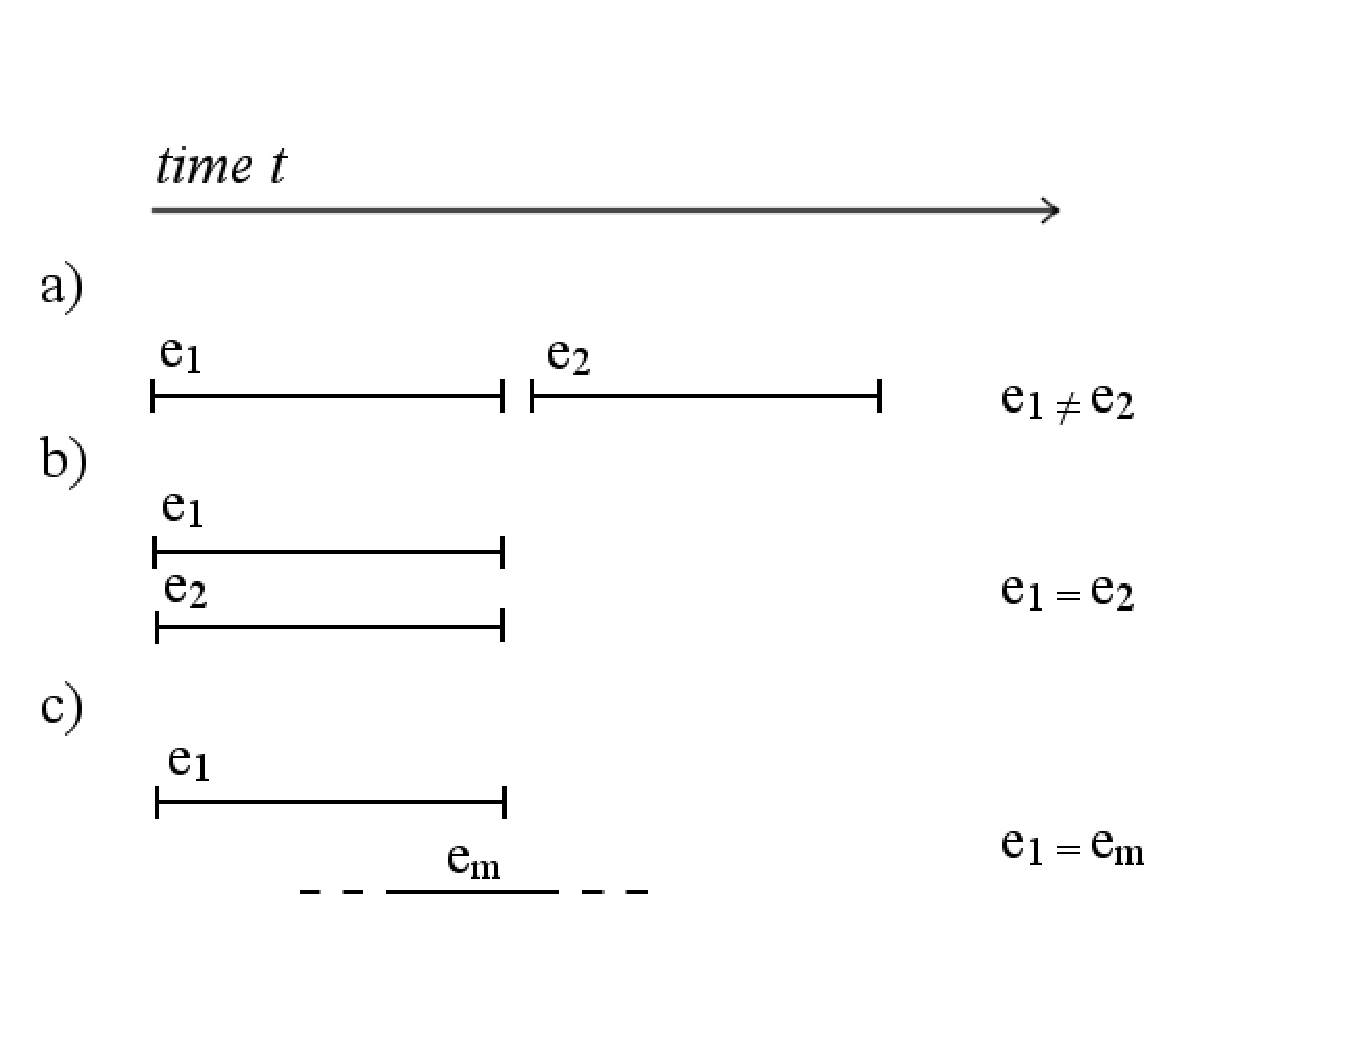
\includegraphics[width=1.0\textwidth]{figures/eventschemav2.eps} 
\caption{Interaction types between event arguments in MVCs}\label{fig:events}
\end{figure}

At this point, using event arguments does not reveal any explanation as to why the LLEs in type a) do not merge but constitute a staged CLE, while the LLEs in b) do so. But assuming event arguments to be active in the formation of MVCs does provide us with a means to be able to model different temporal configurations.

The next section will have a closer look at lexical decomposition which is particularly helpful when it comes to  merger scenarios as for example \textsc{merging} of motion events in (\ref{WMH_Julio_goat049_2}). Before I close this section, however, I would like to address a further quirk to the event argument analysis. As it turns out, MVCs do not only provide event arguments on the LLE level, they also seem to produce more complex event arguments on higher levels (and thereby arguably confirm the existence of PLEs and CLEs). This becomes clear when MVCs are inserted into Maienborn's event diagnostics listed in (\ref{diagnostics}) above. The first test claims that, as events are perceptible in space and time, linguistic construals of events are permitted to occur as (infinitical) complements in perception verb constructions. If we have a look at the EI area it turns out that this idea is also applicable to MVCs. In Wooi for instance, motion-to-action constructions may occur as complements of perception verbs just like simplex predicates do. Consider the following elicited example (note that the English translation uses an infinitive construction for readability (``accusative and infinitive" in Latin Grammar) - the original structure in Wooi does not support a raising hierarchy):

\ea \label{hendeho}
\langinfo{Wooi}{Autronesian, SHWNG}{elicit.}
\ea
\glll hende ho kiori ra con ho i \\
he-re ho $<$i$>$ko=i ra ti-ong ho i \\
3\textsc{pl}-eye \textsc{dir} $<$3\textsc{sg}$>$carry=\textsc{obj}.\textsc{sg} go 3\textsc{sg}-give \textsc{dir} 3\textsc{sg}\\
\glft `They saw him carry it there and give it to her.' (lit. they saw him carry go give it to her')\\
\ex
\glll *hende ho i kiori ra con ho i\\
he-re ho i $<$i$>$ko=i ra ti-ong ho i \\
3\textsc{pl}-eye \textsc{dir} 3\textsc{sg} $<$3\textsc{sg}$>$carry=\textsc{obj}.\textsc{sg} go 3\textsc{sg}-give \textsc{dir} 3\textsc{sg}\\
\z
\z

The matrix construction in (\ref{hendeho}) is a nominal predicate consisting of the word for eye and a directional. This is the standard way of encoding visual perception in Wooi. All material that comes after the directional belongs to a (complex) motion-to-action MVC that is subordinated as stimulus argument of \textit{hende ho}. The starred sentence confirms that it is indeed the stimulus argument slot that hosts the MVC: the pronoun \textit{i} can act as a substitute for the action to be perceived, but it cannot co-occur with the full argument spelled out by the MVC. The first sentence, on the other hand, is absolutely fine, as would be \textit{hende ho i} 'They saw it'.

Maienborn's second test for hidden event arguments claims that event expressions combine with locative and temporal modifiers. This test accords less well with MVCs from Eastern Indonesia. First and foremost, neither locative nor temporal modifiers typically occur with MVCs which is most probably due to their specific pragmatic function. MVCs tend to be used to sum up paragraph information by repeating the previously introduced verbs in a compressed formula. At the point of the MVC wrap-up, temporal or locative information are usually already known from previous utterances and tend to get dropped during the summarising part. This is why the dataset does not contain many examples of MVCs modified with locative or temporal adverbials. If indeed such modifiers co-occur with MVCs the scope is typically confined to one of the stages. Consider the following rather complex MVC from Wooi.

\ea \label{} 
\langinfo{Wooi}{Austronesian, SHWNG}{frogstory\_Kosmus}\\
\glll hunda huna husa haherai na wirey \\
hu-ra hu-na hu-ha hahera=i na wirey \\
3\textsc{du}-go 3\textsc{du}-be.at 3\textsc{du}-call search=\textsc{obj}.\textsc{sg} \textsc{loc} forest\\
\glft `Both of them went out into the forest and searched (for the frog).' \\
\z

The whole construction is a motion-to-action MVC on the matrix level, that is, it consists of a precursor motion stage followed by an action stage. Although the forest is by way of inference the goal of the going, the scope of the locative PP \textit{na wirey} at the end is in all likelihood only on the action phase \textit{huna husa haherai} (given the setting in the frogstory, and the specific context of the narration). This illustrates that locative modifiers should provide a good way of testing whether a given MVC is staged (that is, whether it contains two temporal phases) or not. With staged MVCs, the natural scope of the modifier is only on one of the stages, typically the one that is closest to the modifier. Some staged MVCs, however, seem to be ambiguous between two scope interpretations. For instance, resultative MVCs such as the one in example (\ref{keriaviata}) would probably be interpreted as being jointly modified by the locative adverbial, with both stages being inside its scope. But this would need to be tested (for instance with entailment tests), so that I can only suggest such an assumption at this point. Note, however, that such MVCs convey the strong reading of immediate sequence, suggesting that a reading along the lines `die at (unspecified) place x, and remain at place y' would probably be dispreferred, or even impossible.

\ea \label{keriaviata} 
\langinfo{Wooi}{Austronesian, SHWNG}{poison\_for\_animals}\\
\glll keria via na vavaw \\
$<$i$>$karia $<$i$>$va na vavaw \\
$<$3\textsc{sg}$>$die $<$3\textsc{sg}$>$lie \textsc{loc} there\\
\glft `(The animal) will die and remain there.' (lit. `it will die lie there')\\ 
\z

Maienborn's last test, event expressions combining with manner adverbials, comitatives etc, is also possible with MVCs. Construals of motion, for instance, can be targeted by adverbials like \textit{slow} or \textit{fast} (which are usually also regarded as verbs in most of the EI languages). Have a look at the next example from Wooi. Stative verb \textit{mararu} is placed right before a \textsc{motion complex} consisting of the two verbs \textit{vavu} `return.home' and \textit{taveri} `return' (the latter of which does not receive subject indexing in this constructional slot). As both motion verbs contribute facets to the overall motion event, \textit{mararu} targets the whole construction. If modifiers such as \textit{mararu} are argued to operate over a hidden event argument, then it would seem that in (\ref{Wooi41}) the event arguments of both verbs act together. This comes very close to what I called PLE above.

\ea \label{Wooi41} 
\langinfo{Wooi}{Austronesian, SHWNG}{HIVIAY\_exp 077}\\
\glll tamararu tambavu taveri \\
ta-mararu ta-vavu taveri \\
1\textsc{pl}.\textsc{in}-fast 1\textsc{pl}.\textsc{in}-return.home return\\
\glft `We go home fast.' \\ 
\z

What these tests suggest is that MVCs may not only provide LLEs with a hidden event argument but that these event arguments can be bundled and interpreted as one composite event argument, at least with some construction types in some of the languages. Our event argument model that I sketched out in Figure \ref{fig:eventsmod} may therefore be extended in the following way in order to capture the range of variation in MVC event construals.

\begin{figure}
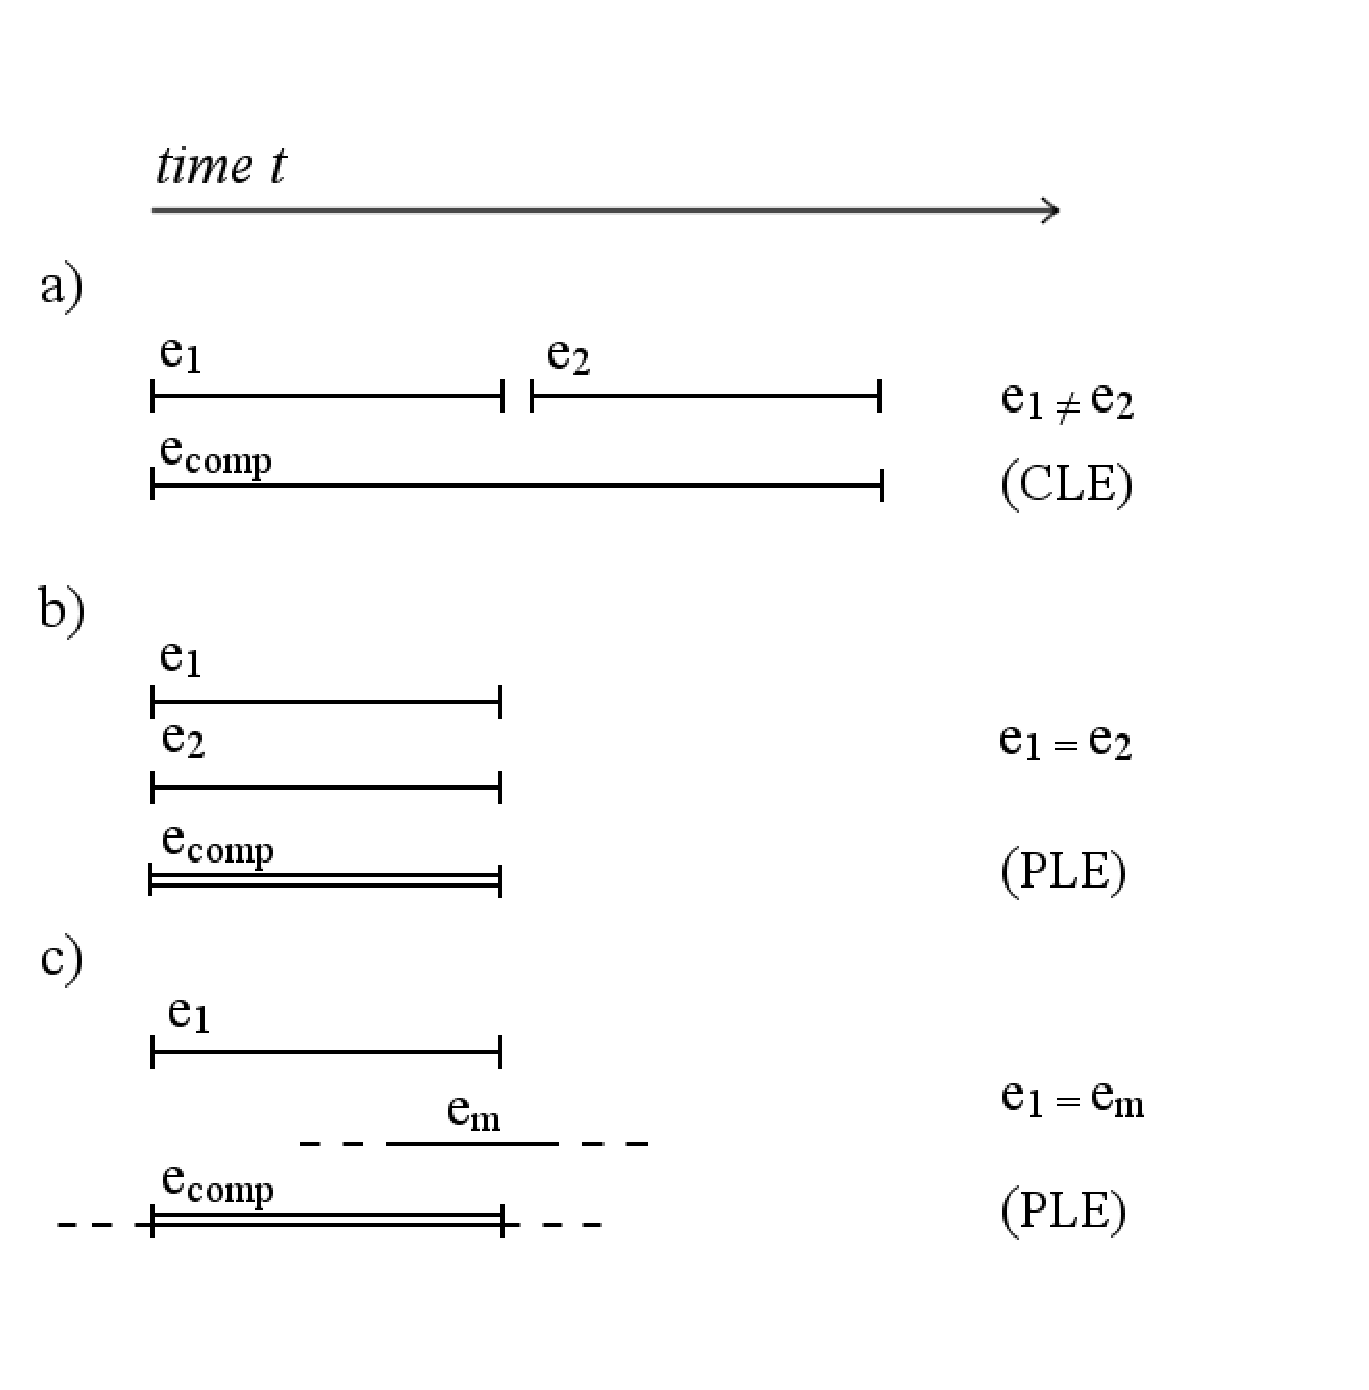
\includegraphics[width=1.0\textwidth]{figures/eventschemamod.eps} 
\caption{Interaction types between event arguments in MVCs, resulting in composite event arguments.}\label{fig:eventsmod}
\end{figure}


The a) type again is the staged MVC. The event arguments of both verbs are joined together on the clausal level (yielding a CLE), a result that appears also to follow from the fact that the overwhelming majority of such constructions show shared operator scope with grammatical formatives, targeting a composite event schema rather than the underlying LLEs of the verbs. Type b) represents merger MVCs that only consist of one temporal stage. Here, both event arguments can be thought of as being projected on each other (or, to be more precise, $e_2$ fuses with matrix event $e_1$). The resulting composite event (argument) is rooted in the predicate level rather than being aligned with the clausal level (mostly because such construals are allowed to enter stages of higher-level MVCs). The same goes for the modifying type c) where the matrix verb exerts spatiotemporal limits on the modifier thus making its event schema $e_m$ fit into the spatiotemporal frame of $e_1$.

\subsection{Lexical decomposition} \label{sec:decomposition}

It has become clear from the last section that hidden event arguments may motivate different spatiotemporal templates in MVCs, yet they cannot fully explain why staged MVCs do not have their LLEs combined while non-staged MVCs might do so. To this end, this section reviews another semantic approach that might help out in this matter.

Ever since Vendler it has been clear that verbs fall into different event classes. Walking an unspecified distance is different from reaching a summit, or from building a house. This difference in lexical aspect can be demonstrated by applying different grammatical tests, such as using the progressive aspect in English, or adding a temporal frame adverbial such as \textit{for x time} or \textit{in x time}. The different verb classes show different reactions to these tests thereby justifying the well-known distinction into \textit{states}, \textit{processes} (or \textit{activities}) and \textit{events} (or \textit{transitions}) (see for instance \citealt{pustejovsky1991syntax} for a concise discussion). The latter category denotes eventualities that have a culmination point beyond which a resultant phase occurs with adversative semantics (for instance, the culmination point of \textit{building a house} is the point in time when the house is built). The classical distinction in \citet{vendler1957verbs} is between \textit{achievements} that occur punctually and are typically non-agentive, and \textit{accomplishments} with a durative phase leading up to the culmination point. As opposed to \textit{achievements}, \textit{accomplishments} are volitional actions driven by a willful instigator (building a house would hardly be imaginable without a clear agent).

Another insight from verb class analysis is that one and the same verb may be associated with different verb classes. This is the case with verbs that allow for different argument patterns. If we say that \textit{the door is closed}, we refer to a state of indefinite temporal extension, while \textit{the door closed} would involve a state change between the door being not closed and the door being closed. A construction like \textit{Jones closed the door} would involve a transitive configuration, specifying an actor that causes the state change from $\neg$closed to closed. Another way of `pushing' a verb into another verb class is by adding non-verbal constituents (NPs, PPs, adverbials and so on) to it that alter the event interpretation. An event of \textit{eating apples}, for instance, could go on for quite some time, while \textit{eating an apple} is clearly bound by the size of the apple (and the appetite of the eater). From an event perspective, however, \textit{eating an apple} seems to be quite the same event as, say, \textit{painting a picture}, or \textit{digging up a parsnip}. The central idea with lexical decomposition is to assign a common sublexical structure to all such instances of the `same' event class in order to explain their identical aspectual behaviour.

According to most contemporary theories of lexical decomposition, the structural part of verb meanings basically consists of a stock of primitive predicates (minimal conceptual events with particular predicate-argument configurations) which license primitive objects (basically things, places etc) to fill their argument positions. Such decomposed meaning primitives are thought to constitute what is called the Lexical-Conceptual Structure (short \textsc{LCS}) of a verbal lexeme. The minimal predicates themselves are allowed to enter argument positions licensed by other primitive predicates according to specific rules of combination (referred to, for instance, as Template Augmentation by \citealt[111]{rappaport1998building}). The claim is that by combining these primitive predicates to more complex predicate-argument structures, a potentially universal set of event types can be established that defines the limits of what event conceptualisations verbs are capable to denote \citep{rappaport1998building, baker2010complex}. A decompositional view on the semantic structure of verbs lends itself particularly well to theories of multi-verb interactions. If semantic structure is confined to and made of a smallish set of minimal predicates then in principle verbs that lexicalize part of the same semantic structure can be expected to merge that structure under certain conditions. This is the line of reasoning that \citet{baker2010complex} adhere to in their application of predicate decomposition to Australian coverb constructions and SVCs from a range of other languages. They argue that there is a fundamental distinction between merger constructions fusing part of their event structure, and coindexing constructions where fusion in a quite different sense pertains to the identity of arguments across different verbs. While this approach is certainly a powerful tool to identify the semantic driving force at work in MVCs, much of its explanative power hinges on the type and amount of primitives that are postulated by decomposition theories.

As \citet{levin2005argument} point out, three basic approaches to semantic decomposition may be distinguished: (i) localist approaches, (ii) aspectual approaches, and (iii) causal approaches. All three of them have focused on specific semantic features (roughly, the semantics of space, time, and reason, or force, respectively) and while all of them have successfully dealt with subsets of verbal predicates, no approach is without shortcomings when it comes to other parts of the verbal lexicon. In what follows I will focus on the localist and aspectual approaches to lexical decomposition, while more or less ignoring the causal approaches (basically because the former two appear to be more suitable to MVC analysis). While both spatial and temporal decomposition are valuable tools with regard to certain verb classes, they are not capable of modelling \textit{all} classes equally well. For instance, localist approaches are great with motion and position verbs but quite bad at motivating the internal structure of, say, verbs of change of possession such as \textsc{take} or \textsc{give}. Therefore, most current takes on verbal decomposition rather make use of a hybrid set of semantic primitives, drawing from ideas from different approaches. In what follows I will give a short account of some of the basic tenets of localist and aspectual approaches, and point out some of their drawbacks when they are applied in a pure fashion. In §\ref{sec:sem-templates}, I will then sketch an approach to model verb classes which is basically informed by what \citet{van1997syntax} present as a semantic decomposition of verb classes within the RRG framwork. I will need to add some further primitives into the Van Valin and LaPolla system in order to account for the MVC data und the specific behaviour of EI merger constructions.

\subsubsection{Spatial decomposition}

The localist approach claims that the most fundamental cognitive concepts involve the semantic field of motion and location, and that most conceptual semantic structures can be modeled by use of primitives such as \textsc{go}, \textsc{be}, and \textsc{stay}. The localist approach dates back to work by \citet{gruber1965studies}, followed and formally elaborated by \citet{Jackendoff1990}, and has recently been used by \citet{baker2010complex} to motivate their distinction between verbs that undergo predicate merging and other multiverb constructions that involve mere coindexing of shared arguments. The localist approach is particularly good at accounting for all those domains in verb semantics in which a theme is located somewhere or is in motion along a path, including many instances of metaphorical constructions of motion and location in other semantic fiels. Consider the following examples, taken from \citet[25]{Jackendoff1990}:

\ea \label{Jackendoff01} Spatial location and motion
\ea  The bird went from the ground to the tree.
\ex The bird is in the tree.
\ex Harry kept the bird in the cage.
\z
\z

\ea \label{Jackendoff02} Possession
\ea The inheritance went to Philip.
\ex The money is Philip's.
\ex Susan kept the money.
\z
\z

\ea \label{Jackendoff03} Ascription of properties
\ea The light went/changed from green to red. \\
Harry went from elated to depressed.
\ex The light is red. \\
Harry is depressed.
\ex Sam kept the crowd happy.
\z
\z

While the examples in (\ref{Jackendoff01}) illustrate basic construals of motion and location, other semantic fields as well show similar ways of construal. Take for instance the semantic field of possession illustrated in (\ref{Jackendoff02}): possessed referents can be 'moved' from one participant to another, adessive construals of possessor and possessee are a typologically frequent way of expressing alienable possession, and so on. The same metaphorical connection to construals of motion and location holds for many other semantic fields and is proposed to inherently underly such predicate classes as change of state predicates, states, and predicates of prolonged engagement (cp. (\ref{Jackendoff03})), demonstrating the pervasive role scenarios of motion and location play in human cognition. According to the Thematic Relations Hypothesis (\citealt{gruber1965studies}, adapted in \citealt{Jackendoff1990}), both the basic construals of motion and locations as well as the derived ones are claimed to be realizations of the same underlying conceptual functions, illustrated in (\ref{themrel}) \citep[26]{Jackendoff1990}.

\ea \label{themrel}
Basic conceptual functions of motion and location
\z

\avmsortfont{\itshape}
{\scriptsize
\begin{avm}
\sort{Event}{\[
GO 
\( \[ \hspace{20pt} \], \sort{Path}{\[ 
FROM \(\[ \hspace{20pt} \]\) \\
TO \(\[ \hspace{20pt} \]\) \]} 
\) 
\]}
\end{avm}
}

\smallskip
{\scriptsize
\begin{avm}
\sort{State}{\[
BE 
\( \[ \hspace{20pt} \], \sort{Place}{\[ \hspace{20pt} \]} 
\) 
\]}
\end{avm}
}

\smallskip
{\scriptsize
\begin{avm}
\sort{Event}{\[
STAY 
\( \[ \hspace{20pt} \], \sort{Place}{\[ \hspace{20pt} \]} 
\) 
\]}
\end{avm}
}

\bigskip
The conceptual function \textsc{go} has two arguments, a theme argument denoting the entity under motion, and a path argument which in turn may host a set of monovalent path predicates, such as \textsc{from}, \textsc{to}, or \textsc{via}. The two location functions \textsc{be} and \textsc{stay} also denote a theme argument combined with a place. As many verbs appear in constructions that involve motion and/or location subevents, these conceptual functions are frequently used in modeling more complex event structures. To illustrate, take for instance the event semantics of \textsc{putting} some object at some place, apparently including a motion component (the theme that is relocated) and a goal component (the place at which the theme is put to rest). Quite intuitively, the event template of a \textsc{put} predicate would invite the use of the conceptual functions \textsc{go} (or \textsc{move}) and \textsc{be} in order to capture these semantic components. Baker and Harvey propose the following conceptual structure for the merger construction (\ref{Marra03}) in the Australian language Marra, consisting of the coverb \textit{birli} `go in' and the lightverb \textit{ganji} `take' \citep[24f.]{baker2010complex}. The merging results in a combined stucture \textit{birli ganji} which means 'put in':

\ea \label{Marra01}
\textit{birli} `go in': {\small[$_{Event}$ MOVE ([$_{Thing}$ x ], [$_{Path}$ IN ])]}
\z
\ea \label{Marra02}
\textit{ganji} `take': {\small[$_{Event}$ CAUSE ([$_{Thing}$ y ], [$_{Event}$ MOVE ([$_{Thing}$ x ], [$_{Path}$ ])])]}
\z

\ea \label{Marra03}
\textit{birli + ganji} `put in': \\
{\small[$_{Event}$ CAUSE ([$_{Thing}$ y ], [$_{Event}$ MOVE ([$_{Thing}$ x ], [$_{Path}$ IN ])])]}
\z

By combining the event templates of \textit{birli} in (\ref{Marra01}) and \textit{ganji} in (\ref{Marra02}) to the joint conceptual structure of \textit{birli ganji} in (\ref{Marra03}), the functions \textsc{cause} and \textsc{move} enable the theme argument x to be transferred by the causing referent y along a path \textsc{in} to a place inside a container, where \textsc{in} is shorthand for a more complex path-goal combination like [\textsc{to} [\textsc{in} $<$place$>$]] (see \citealt[45]{Jackendoff1990}). The lightverb \textit{ganji} provides the structural skeleton of a three participant event construal (causer, theme, and path), while the coverb \textit{birli} contributes specific content on the motion path traversed by the theme. 

Evidently, the use of \textsc{go} (or \textsc{move}, for that matter\footnote{In the following discussion and throughout the book, I regard \textsc{go} and \textsc{move} essentially as synonymous notations for a predicate function that involves physical motion or movement and licenses a path argument (see also \citealt[27]{baker2010complex} for a similar stance)}) seems felicitous iff a verb has among its options of argument expression construals in which it combines with path modifiers, such as \textsc{put} allows in English (as in \textit{Jones put the toast on the table}). However, the claim of the Localist Approach extends beyond verb semantics of physical orientation and seeks to account for many other verb classes where physical motion figures less prominently or may even be absent. This is in particular the case with certain classes of activity verbs and change-of-state verbs where a \textsc{move} component would make wrong predictions with regard to predicate merging. I will illustrate the problem of \textsc{move} generalization with the case of change-of-state verbs. For example, in their discussion of merger constructions in Wagiman (Australian) Baker and Harvey provide the following LCS for \textit{du} `cut':

\ea \label{Wagiman01}
\textit{du} `cut': \\
{\small[$_{Event}$ CAUSE ([$_{Thing}$ ], [$_{Event}$ MOVE ([$_{Thing}$ ], 
[$_{Path}$ TO ([$_{Place}$ IN [$_{Thing}$ ]])])])]}
\z

The transitive argument configuration is modeled by a \textsc{cause} predicate licensing an actor argument, and an embedded \textsc{move} predicate that is further subcategorized for an object and a path function referring to the goal argument of the cutting. The reason for assuming such a LCS is probably that from a spatiotemporal point of conception, the postulation of a path trajectory for an instrument (such as a knife or other object with a sharp blade) dissecting a patient argument makes perfect sense. There is, however, room for doubts whether this trajectorial part is really lexicalized in \textsc{cut} verbs in this way. In particular, two objections may be raised. First, though not commented on directly by Baker and Harvey, the first argument of the \textsc{move} function can only be logically understood as the instrument of cutting. As argument slots licensed by predicate functions ought to map on morphosyntactic arguments, we would need to expect that the instrument as such is realized as a subcategorized argument rather than an instrument adjunct. That is, at least one of the event templates \textsc{cut} occurs with should display an instrument phrase in object function combined with a path argument. One way to put the semantic structure to a test is to look at the licit patterns of argument realisation of \textsc{cut} verbs. Starting with the work of \citet{Fillmore1970}, verb classes in English and other languages have often been analysed and argued for by virtue of comparing so called diathesis alternations, specific alternations in the morphosyntactic expression of arguments, which verbs of the same verb class participate in \citep{Levin1993}. Verbs of \textsc{hitting}, \textsc{breaking}, and \textsc{cutting} have received major attention because unlike their basic transitive make-up suggests these verb classes differ in specific ways by permitting specific subsets of these alternations. Consider the following examples (taken from \citealt[148f. and 156]{Levin1993}):

\ea Basic transitive argument realization \label{alt01}
\ea Carol hit the fence
\ex Carol cut the bread
\z
\z

\ea Instrument Subject Alternation \label{alt02}
\ea Carol hit the fence with a stick
\ex Carol hit the fence
\ex Carol cut the bread with a knife
\ex Carol cut the bread
\z
\z

\ea Middle Alternation \label{alt03}
\ea[*]{The fence hits easily}
\ex[]{Paula hit the fence}
\ex[]{Whole wheat bread cuts easily}
\ex[]{Carol cut the whole wheat bread}
\z
\z

\ea With/Against Alternation \label{alt04}
\ea[]{Carol hit the stick against/on the fence}
\ex[]{Carol hit the fence with the stick}
\ex[*]{Carol cut the knife against/on the bread}
\ex[]{Carol cut the bread with the knife}
\z
\z

The basic transitive construction in (\ref{alt01}) is fine with both the \textsc{hit} and the \textsc{cut} class, and so is the Instrument Subject Alternation in (\ref{alt02}) where an instrument adjunct is added. The alternations given in (\ref{alt03}) and (\ref{alt04}), however, are only applicable to one of the two classes: while \textsc{cutting} allows the Middle Alternation in which the patient argument is promoted to subject function, the \textsc{hitting} class does not. The reverse is true for the With/Against Alternation where the instrument argument is promoted to direct object function and the patient argument is realized as oblique. It is particularly this alternation that is interesting in the light of the predicate decomposition of Wagiman \textit{du} `cut' above: as the alternation shows, \textsc{hit} verbs do lexicalise an instrument-path template in which the instrument is moved along a path on a patient argument. Therefore, \textsc{hit} verbs may well receive the same predicate decomposition as for instance relocation verbs such as `put' in (\ref{Marra03}) above. \textsc{cut} verbs, on the other hand, do not seem to offer such an instrument-path template and are therefore probably better analysed as change-of-state verbs involving an activity or accomplishment decomposition by making use of a [CAUSE [BECOME [BE]]] combination.

The second objection that may be raised against a localist decomposition of \textsc{cut} verbs directly pertains to  predictions of predicate merging that would follow from a \textsc{move} component. In my Eastern Indonesian sample, several transitive verb classes are attested that are open to verbal path modification provided by a motion verb in V$_2$ position. According to the glosses used in the data, \textsc{hit} verbs, \textsc{take} verbs, object relocation verbs such as \textsc{put} or \textsc{pour}, verbs of force exertion (\textsc{pulling} and \textsc{pushing}), and other transitive verbs like verbs of directed sensual perception may be modified in such a way (possibly with different languages allowing different verb classes to undergo verbal path modification). \textsc{cut} verbs, however, are not among them which suggests that they function differently from verbs that directly lexicalise path components as basic part of their meaning.

Therefore, I conclude that a cogent analysis using predicate decomposition to motivate the formation of certain kinds of multi-verb constructions would need to base the semantic templates on the morphosyntactic behaviour of the constructions attested in the sample. Localist predicate decomposition develops a particularly strong explanative force with those construals in which the patterns of argument realisation closely mirror the proposed underlying predicate semantics. The use of \textsc{move} predicates, however, should be limited to those verbs that either lexicalise a translational motion event or else a movement path pertaining to object relocation (thematic relation), object affection (patientive relation), or directed sensation.
It would seem logical that for those instances in which motion is indeed a valid function to occur in semantic structure, the inference should hold that at the final event boundary, the moving object should have reached its designated place. We may formalise this inference by using Jackendoff's inference rule given in (\ref{Jackendoff04}) and limit its scope to instances of motion proper \citep[27]{Jackendoff1990}:

\ea \label{Jackendoff04} Inference rule \\
At the termination of [$_{\textit{Event}}$ GO ([X], [$_{\textit{Path}}$ TO ([Y])])], \\
it is the case that [$_{\textit{State}}$ BE ([X], [$_{\textit{Place}}$ AT ([Y])])].
\z

Thus, strictly speaking if Jones cuts a bread into slices it is not the case that either Jones or the bread partake in a motion event (and the knife as a moving instrument should be ruled out from filling the argument position [X] on the basis of the evidence from diathesis alternations sketched above). This is not to say that motion is totally absent from the event conceptualisation of cutting. Most if not all dynamic events may involve motion conceptualisations of some sort. Yet, I think that it is only with certain verb classes that motion as a templatic feature takes centerstage in event lexicalisation.

\subsubsection{Aspectual decomposition}

Another approach to predicate decomposition is rooted in theories of aspectual verb classes. The aspectual approach starts out from the by now classical observations into lexical aspect initiated by Vendler's work on verb classes in English: the differentiation of states, acitivites, achievements, and accomplishments basically revolves around the notions of stativity, punctuality, and telicity with statives being different from the other three classes by virtue of being stative (or non-dynamic), activities by having no inherent endpoint (being atelic), and achievements by being telic but punctual (without temporal duration) as opposed to accomplishments (see e.g. \citealt{levin2005argument, croft2012verbs}). A typical feature space of the Vendler classes is given in Table \ref{table:Vendler} (taken from \citealt[93]{van1997syntax}).

\begin{table}
\begin{tabular}{lccc}
\lsptoprule
\multicolumn{1}{l}{class}&\multicolumn{1}{c}{static}&\multicolumn{1}{c}{telic}&\multicolumn{1}{c}{punctual}\tabularnewline
\midrule
State&+&\textminus&\textminus\tabularnewline
Activity&\textminus&\textminus&\textminus\tabularnewline
Accomplishment&\textminus&+&\textminus\tabularnewline
Achievement&\textminus&+&+\tabularnewline
\lspbottomrule
\end{tabular}
\caption[Feature combination of Vendler verb classes]{Feature combination of Vendler verb classes (from \citealt[93]{van1997syntax})}
\label{table:Vendler}
\end{table}

The most important evidence for the feature combinations shown in Table \ref{table:Vendler} comes from insertion tests, starting with Vendler's seminal study \citep{vendler1957verbs}. Each feature is tested by constructing a carrier frame or by applying a grammatical category to the verb: the stative/dynamic distinction can be shown by applying the English progressive which is acceptable for dynamic verbs but not for statives. For example, while \textit{I am running} is a well-formed answer to the carrier question \textit{What are you doing?}, \textit{*I am knowing it} is definitely not \citep[35]{croft2012verbs}. The punctual/durative distinction can be tested by applying temporal question pairs such as \textit{At what moment...?} vs \textit{For how long...?}. Achievement verbs like \textit{spot} only license a punctual time frame (cp. \textit{At what moment did you spot the plane?} and \textit{*For how long did you spot the plane?}, op.cit.) in contrast to the other verb classes which are prototypically construed with a durative time frame (but see \citealt{croft2012verbs} for alternative construals). Finally, the atelic/telic or unbounded/bounded distinction becomes apparent when temporal adverbials are added: with durative temporal adverbials such as \textit{for ... [time]} in English, no natural endpoint is implied and the event may end without having reached a state change. Thus, construals of activity verbs as in \textit{He pushed the cart for half an hour} are fine, while construals with accomplishment verbs as in \textit{?She drew the circle for half an hour} seem odd (yet here again, alternative construals are available for some verbs). Construals involving the container adverbial \textit{in ... [time]} just show the reverse pattern. While they readily modify bounded/telic verbs (cp. \textit{She drew the circle in twenty seconds}), construals of activity verbs are generally rejected (with the exception of activity verbs that allow for an accomplishment construal, such as \textit{*Erin ate in two minutes} vs \textit{Erin ate the apple in two minutes}, see \citealt[99]{van1997syntax} and \citealt[38]{croft2012verbs}). In more recent work on lexical aspect, more fine-grained class distinctions have been proposed yet the original four Vendler classes still constitute the backbone of most aspectual approaches to verb semantics. \citet{croft2012verbs} provides a comprehensive overview of the different subclasses and additions proposed in the literature.

Aspectual approaches to verb decomposition take the idea of aspectual verb classes as a vantage point for deconstructing verbal semantics. The conceptual primitives that are used to model the aspectual classes include \textsc{be} for stative verbs, \textsc{do/act} for activity verbs, and \textsc{become} (and \textsc{ingr}(essive) in Van Valin and LaPolla's RRG framework) for bound verbs (achievements and accomplishments). Unlike in the localist approach, the notions of motion and position are not granted the status of independent semantic functions in aspectual frameworks but are subsumed as subsets under different aspectual classes. This has some advantages and at the same time poses certain difficulties. For instance, \citet[106]{van1997syntax} point out that motion path verbs like \textsc{come} and \textsc{go}, contained motion verbs like \textsc{enter}, and motion ground verbs such as \textsc{arrive} may conceptualise either punctual or durative events in different languages. This variation in temporal extension is probably better captured within an aspectual verb class model where the class distinctions directly reflect the temporal properties of the event conceptualisations. To illustrate the point, manner of motion verbs can be construed both as atelic activity verbs and as telic accomplishments depending on the arguments realized in the clause. One solution to this variation is to make use of semantic functions that directly pertain to the aspectual type of event. Consider the following examples from \citet{van1997syntax}:

\ea \label{VanValin:run}
\ea Paul ran. \label{VanValin:runa}
\exi{a'} \textbf{do'}(Paul, [\textbf{run'}(Paul)])
\ex Paul ran to the store. \label{VanValin:runb}
\exi{b'} \textbf{do'}(Paul, [\textbf{run'}(Paul)]) \& \textsc{become} \textbf{be-at'}(store, Paul)
\z
\z

In example (\ref{VanValin:runa}) the event of running is construed as an unbound activity since no argument is realized that would impose a temporal boundary on the event. The atelic activity reading is directly reflected by use of the empty activity predicate \textbf{do'}. In example (\ref{VanValin:runb}), on the other hand, the running event is temporally delimited to the distance from the starting point up to the place of the store. The telic reading of this predicate is accounted for by adding a second accomplishment predicate to the activity, connected through the predicate connective '\&'. The advantage here is obvious: running in its activity reading directly classes with other activity predicates like \textsc{eat}, \textsc{sweep}, \textsc{talk} and so on. By contrast, localist approaches cannot deal with activity verbs in such a straightforward way. To give just two examples, consider the semantic templates for \textsc{walk} (\ref{Baker:walk}) and \textsc{eat} (\ref{Baker:eat}) as proposed by \citet{baker2010complex}\footnote{For sake of convenience, I adopt a simplified notation of Jackendoff's, and Baker and Harvey's framework from now on. Specifically, I only make use of the square brackets [ ] in cases where they increase the overall readability of the formula, i.e., when an argument itself contains a predicate with a set of subcategorized arguments. Also, I don't give subscribed labels such as \textit{event}, \textit{thing}, or \textit{place} as they are mostly inferable from the structural position.}:

\ea \label{Baker}
\ea \textsc{move} (x, \textsc{path}) \label{Baker:walk}
\ex \textsc{cause} (x, [\textsc{move} (y, \textsc{path})]) \label{Baker:eat}
\z
\z

Baker \& Harvey propose a generic \textsc{move} predicate to account for activity predicates, roughly following Jackendoff's  localist analysis (though conflating \textsc{move}(x) and \textsc{go}(x,\textsc{path}) into a single primitive \textsc{move}). Intransitive activity predicates generally follow the schema depicted in (\ref{Baker:walk}). The subscribed semantic content of the verb complements the generic function \textsc{move}, realized with a subject referent x and optionally a path component. Transitive activity verbs, such as \textsc{eat}, however, are rendered in a different manner in order to capture the difference in argument frame (actor plus patient argument). Here, the actor argument is licensed by the predicate \textsc{cause} which as a second argument takes the activity configuration \textsc{move}(y,\textsc{path}). The latter, however, can hardly be thought of as constituting an independent activity predicate as it might be expected from a comparison with, say, break verbs that allow for the causative alternation, cp. \textit{The thief broke the window} vs. \textit{The window broke}. There is no such alternation for \textsc{eat} in English that would provide evidence for an analysis along the lines of (\ref{Baker:eat}). While the Unspecified Object Alternation is fine (\textit{Cynthia ate the peach} vs. \textit{Cynthia ate}; \citealt[213]{Levin1993}) no such alternation is possible between a transitive argument realization (\textit{Cynthia ate bread}) and an intransitive one with the patient being promoted to subject position (\textit{*The bread eats})\footnote{The middle alternation, on the other hand, seems licit in certain contexts, for example \textit{This bread eats like a meal} (google search). Using a \textsc{cause} function to model transitive activity/accomplishment predicates is also problematic for another reason as analytical causatives like \textit{Peter made Cynthia eat the bread} would derive a predicate structure with two instances of causing, Peter causing Cynthia to eat, and Cynthia causing the bread to move. That extensive use of \textsc{cause} in lexical decomposition would give rise to problems of that kind has also been noted by \citet{Jackendoff1990}.}. In aspectual approaches like \citet{rappaport1998building} or \citet{van1997syntax} the challenge posed by transitivity contrasts is deferred to the semantic content. Compare the examples in (\ref{VanValin:drink}) from \citet[111]{van1997syntax}:

\ea \label{VanValin:drink}
\ea Carl drank beer. \label{VanValin:drinka}
\exi{a'} \textbf{do'}(Carl, [\textbf{drink'}(Carl, beer)])
\ex Carl drank a beer. \label{VanValin:drinkb}
\exi{b'} \textbf{do'}(Carl, [\textbf{drink'}(Carl, beer)]) \& \textsc{become} \textbf{consumed'}(beer)
\z
\z

Instead of introducing an internal \textsc{cause} function (as opposed to external \textsc{cause} functions as in \textit{Floyd made Carl drink the beer}) to the semantic template, the transitive argument configuration of the drinking event in (\ref{VanValin:drinka}) and (\ref{VanValin:drinkb}) is reflected by the way the activity class is built: the empty activity predicate \textbf{do'} takes as arguments both an actor and an action. This action slot is filled with the original semantic content of the predicate in question (here \textbf{drink'}(x,y)), displaying either an intransitive or a transitive subcategorization frame. Modeling transitive activity predicates this way retains a unique activity template and confirms the identical behaviour of activity verbs that is evidenced by the Vendler tests (\textit{What are you doing? I am running/I am drinking beer}). 

A further advantage of Van Valin and LaPolla's system is that by addition of a change-of-state predicate the distinction in aspectual construal between activity and accomplishment readings in (\ref{VanValin:drink}) comes out most clearly. At the same time, however, this practice of suffixing additional semantic functions has some untoward effects on the arrangement as well as the interpretation of the logical structure of predicates. First, any addition to the structure might conflict with the assumption that any material in the event structure should match with syntactic constituents. For example, in terms of well-formedness conditions on the syntactic realization of event structures, \citet[112]{rappaport1998building} propose the Subevent Identification Condition:
 
\ea \textbf{Subevent Identification Condition:} Each subevent in the event structure must be identified by a lexical head (e.g., a V, an A, or a P) in the syntax 
\z

If we apply this condition to example (\ref{VanValin:drinkb}) above, it is not immediately clear which part of the syntactic structure would identify the change-of-state subevent \textsc{become} \textbf{consumed'} (beer). The only structural difference between (\ref{VanValin:drinka}) and (\ref{VanValin:drinkb}) is the use of the indefinite article but even if we assume a DP with the determiner acting as its head (the general rule would then be something like: any countable (number of) object(s) would turn an activity predicate into an accomplishment predicate) the question would remain how \emph{activity} readings with a specified object referent could be dealt with (for instance, with progressives: \textit{Carl was drawing a circle}/\textit{Carl was drawing a circle for ten seconds when suddenly Cynthia distracted him}). 

A second unwanted effect appears with motion predicates that take a path argument. If we have another look at example (\ref{VanValin:runb}) above (repeated below as (\ref{VanValin:runbrep})), we recognise that the path semantics again are supplied by addition of a change-of-state event \textsc{become}. 

\ea \label{VanValin:runbrep}
\ea Paul ran to the store. 
\ex \textbf{do'}(Paul, [\textbf{run'}(Paul)]) \& \textsc{become} \textbf{be-at'}(store, Paul)
\z
\z

This is fine as long as the path is understood as being fully traversed to its end. However, it becomes problematic when the path only encodes a \emph{direction} of the motion (for instance, when the theme moves \textit{towards} some destination without necessarily reaching it). This is the situation that \citet[569]{dowty1991thematic} has discussed under the label \textsc{holistic theme} where it is not part of \textit{Paul} that changes during the runtime of the event but part of the path \textit{to the store} that is traversed. If the semantic content itself, i.e., the motion predicate, wouldn't license a path argument in and of itself where do we get it from if the path is not fully traversed (that is, no state change \textsc{become} \textbf{be-at'} is actually reached)?  Compare the following examples from English and German:

\ea
\ea Paul ran to the store.\label{runstorea}
\ex Paul was running to the store when he realised that he had forgotten his wallet.\label{runstoreb}
\z
\z

\ea \label{runstoreag}
\ea
\gll Paul rannte zum Laden\\
Paul run:\textsc{3}\textsc{sg}.\textsc{pst} to.\textsc{def} shop \\
\glft 'Paul ran to the store.'\\
\ex \label{runstorebg}
\gll Paul rannte zum Laden, aber er kam dort nicht an.\\
Paul run:\textsc{3}\textsc{sg}.\textsc{pst} to.\textsc{def} shop but he arrive:\textsc{3}\textsc{sg}.\textsc{pst} there not \textsc{ptl} \\
\glft 'Paul ran to the store but he never reached there.'\\
\z
\z

In (\ref{runstorea}) and (\ref{runstoreag}), the path argument creates an accomplishment reading by default and it is assumed that Paul finally got there. In (\ref{runstoreb}) and (\ref{runstorebg}), however, the reading of the path argument is atelic and the full path is not necessarily traversed by the actor/theme. In the English example, it is the choice of the progressive aspect that neutralizes or backgrounds the telicity typically brought about by path arguments. Therefore, we may add a temporal clause stating that in the process of traversing the path to the store something else happened and that this may have led Paul to abort his action. In German, the accomplishment reading may even be disabled within the same tense without employing any overt aspect operator. The crucial point is here that by encoding the path argument of certain predicates as an additional change-of-state function complications arise that could be avoided if the path argument would be licensed directly in the semantic structure of the predicate, as is done in localist approaches to predicate decomposition.

In the light of the EI data that I will present below, the best solution would be to assume that path specifications to motion or movement events are directly encoded within the semantic structure of the verb. At the same time it would be detrimental to assume \textsc{move}, \textsc{stay} or \textsc{be} components for all predicate classes as this would basically allow the merging of motion components between almost all predicates and thus would strongly reduce the predictive power of any component-matching model. However, the EI data clearly suggest that merging of semantic structure only occurs between certain verb classes.

Wrapping up the discussion so far, we have seen that localist and aspectual approaches to lexical decomposition both have qualities that make them the best choice with certain verb classes. Localist approaches perform particularly well with verbs permitting path expressions and locative arguments. Aspectual approaches, on the other hand, gain from their ability to directly account for differences in the temporal coding of events and perform better with the original Vendler classes such as activities, or change-of-state predicates. Given that each approach has its own strength, most current frameworks actually combine functions of both strands, forming mixed approaches to lexical decomposition. The next section presents an outline of such a hybrid approach. It is mostly based on Van Valin and LaPolla's system yet includes also some further variables and subclasses that will allow modelling of MVC behaviour in the EI area, as I will show in the subsequent sections.

\subsubsection{Semantic templates in MVC analysis} \label{sec:sem-templates}

In the preceding section, discussion of the path semantics in examples like (\ref{runstoreb}) or (\ref{runstorebg}) revealed that it seems preferential for certain verb classes to include an inherent option for a path expression into their LS. I proposed that there are verb classes in which a general ability of licensing path projections is entrenched somewhere in their lexical representation. In the present section, I will suggest a way in which the insights from localist approaches, i.e. assuming path arguments to be part of a LS) can be combined with a decomposition model that is based on aspectual verb classes. To this end, I will basically use the notational system of \citet{van1997syntax} and add to it additional `empty' predicate functions in order to model the possible fusion scenarios between different classes of EI verbs. I will show that these structural predicates accord with some of the subclasses associated in \citet{van1997syntax} with specific sets of thematic relations. Table \ref{table:semtemp} gives a list of the different semantic templates assumed by Van Valin and LaPolla, complemented with additional predicate functions that I assume in order to account for the MVC merging scenarios.

\begin{table}
\begin{tabular}{ll}
\lsptoprule
\multicolumn{1}{l}{Verb class}&\multicolumn{1}{l}{Semantic template}\tabularnewline
\midrule
State&\textbf{pred'} (x) or (x,y)\tabularnewline\tabularnewline
Activity&\textbf{do'} (x, \textbf{pred'} (x) or (x,y))\tabularnewline
Motion activity&\textbf{do'} (x, \textbf{move'} (x, \textsc{path}, \textbf{pred'} (x) or (x,y)))\tabularnewline
Speech activity&\textbf{do'} (x, \textbf{say'} (x, \textsc{scont}, \textbf{pred'} (x)))\tabularnewline\tabularnewline
Achievement&\textsc{ingr} \textbf{pred'} (x) or (x,y) or\tabularnewline
&\textsc{ingr} \textbf{do'} (x, \textbf{pred'} (x) or (x,y))\tabularnewline\tabularnewline
Accomplishment&\textsc{become} \textbf{pred'} (x) or (x,y)\tabularnewline
&\textsc{become} \textbf{do'} (x, \textbf{pred'} (x) or (x,y))\tabularnewline\tabularnewline
Causative&$\alpha$ \textsc{cause} $\beta$ where $\alpha$, $\beta$ are LSs of any type\tabularnewline
\lspbottomrule
\end{tabular}
\caption[Semantic templates of verb classes, based on \citet{van1997syntax}]{Semantic templates of verb classes, based on Van Valin and LaPolla's lexical respresentations for Aktionsart classes \citep[108]{van1997syntax}.}
\label{table:semtemp}
\end{table}

Van Valin and LaPolla's lexical representations consist of two basic components: constants and variables. Constants are given in boldface and are marked by a prime. Variables are printed in normal typeface. Each constant symbolizes a predicate and is associated with a set of arguments. States and activities are understood as the most basic verb classes. States are represented by a single \textbf{pred'} function, activities are composed of an empty activity predicate \textbf{do'} that takes two arguments: the x argument denotes the effector of the activity (where effector stands for any role within the set of actor-like roles that are licensed by activity verbs), and another argument slot that is filled by the actual predicate constant \textbf{pred'}. The empty activity predicate \textbf{do'} basically acts as the marker of membership in the aspectual class of activites and submits additional information on the thematic role of the first argument x (see \citealt[103f.]{van1997syntax} for reasons to assume an empty \textbf{do'}). Note that the two \textbf{pred'} constants in states and activities are not meant to designate the \emph{same} set of predicates. Rather, the members of the activity \textbf{pred'} typically exclusively occur with \textbf{do'} \citep[103]{van1997syntax}. States and activities are thus mutually exclusive inasmuch as that neither can be derived from the other\footnote{There are, however, exceptions to this in Van Valin and LaPolla's analysis, for instance in their treatment of perception verbs. While seeing is treated as a two-place state, looking is proposed to possess a derived structure containing the same \textbf{pred'}. Consider example (\ref{look}) from \citet[121]{van1997syntax} where the perception state is inserted into an activity LS.

\ea \label{look}
\ea Tanisha looked at the comet with a telescope.
\ex \textbf{do'} (Tanisha, [\textbf{see'} (Tanisha, comet) $\wedge$ \textbf{use'} (Tanisha, telescope)])
\z\z

}

This is why states and activities are analysed as basic verb classes whereas achievements, accomplisments and causative predicates are secondary classes: they either take states or activities as their base. The derivation process of achievements and accomplishments is represented in Van Valin and LaPolla's system by addition of a semantic modifier. Both modifiers take as input a state or activity predicate and derive a telic predicate structure: \textsc{ingr}(essive) marks a punctual change as is commonly associated with Vendlerian achievements, and \textsc{become} denotes a phasic change in which a state change is gradually achieved over time. Examples for each verb class are given below (taken from \citealt[105]{van1997syntax}):

\ea
\ea \textit{States} \\
\begin{tabular}{ll}
The window is shattered.&\textbf{shattered'} (window)\tabularnewline
Fred is at the house.&\textbf{be-at'} (house,Fred)\tabularnewline
John saw the picture.&\textbf{see'} (John,picture)\tabularnewline
\end{tabular}
\ex \textit{Activities} \\
\begin{tabular}{ll}
The children cried.&\textbf{do'} (children, [\textbf{cry'} (children)])\tabularnewline
The wheel squeaks.&\textbf{do'} (wheel, [\textbf{squeak'} (wheel)])\tabularnewline
John ate fish.&\textbf{do'} (John, [\textbf{eat'} (John,fish)])\tabularnewline
\end{tabular}
\ex \textit{Achievements} \\
\begin{tabular}{ll}
The window shattered.&\textsc{ingr} \textbf{shattered'} (window)\tabularnewline
The balloon popped.&\textsc{ingr} \textbf{popped'} (balloon)\tabularnewline
John glimpsed the picture.&\textsc{ingr} \textbf{see'} (John,picture)\tabularnewline
\end{tabular}
\ex \textit{Accomplishments} \\
\begin{tabular}{ll}
The snow melted.&\textsc{become} \textbf{melted'} (snow)\tabularnewline
The sky reddened.&\textsc{become} \textbf{red'} (sky)\tabularnewline
Mary learned French.&\textsc{become} \textbf{know'} (Mary,French)\tabularnewline
\end{tabular}
\z
\z


The examples above illustrate the idea that states (and activities) are the base components in derived LSs: the two-place stative predicate \textbf{see'}, for instance, can be turned into a punctual state-change predicate by adding the modifier \textsc{ingr}. In contrast to the empty activity predicate \textbf{do'}, the semantic modifiers \textsc{ingr} and \textsc{become} do not have an argument frame and do not introduce thematic roles so that the thematic role of, say, the sky in the accomplishment example \textit{The sky reddened} is the same as in the underlying stative base form. Empty \textbf{do'}, however, does impose a thematic role on its predicate constant: we know that the children are not only licensed as argument by the predicate \textbf{cry'} but that \textbf{do'} entails that the children in fact effect the whole event (which is arguably not the case for the sky or the balloon, and not necessarily so for John or Mary in the examples above). Yet we can say that the wheel effects the squeaking, and John effects the event of eating fish. In order to decompose verbs into the basic Vendler classes, it is sufficient in the system of Van Valin and LaPolla to assume three devices (empty \textbf{do'} and the two semantic modifiers) that would turn predicate constants into the four classes. It becomes clear from the few examples, however, that these broad classes fall into a range of subclasses with regard to the thematic relations that are expressed by the first (and second) argument. Within the class of activity verbs, the first argument not only denotes a rather unspecific thematic relation \textsc{effector} but may be subclassified on a more fine-grained scale: with motion verbs, for instance, the \textsc{effector} is the moving entity, i.e., the first argument in the LS may be termed \textsc{mover} according to the role of its argument expression in the event \citep[114f.]{van1997syntax}. Another example of a subclass of the role of \textsc{effector} is the first argument in verbs of speaking. Here, the \textsc{effector} of the event includes the thematic relation \textsc{speaker}. 

I mention these two verb classes here since it is precisely these classes, I want to argue, that allow merging of their LS in some of the EI languages. In motion verb combinations, the crucial component is the path which I assume has the status of a semantic argument, and hence should be part of the LS. In combinations of speech verbs, it is the discourse complement, the content of the utterance, that is encoded in V$_2$. Therefore, I regard the speech content (\textsc{scont}) as a given part of the LS of speech verbs, on the same grounds as I regard the path to be an entrenched component of motion verbs. For each of these classes, I want to propose another predicate function, in the spirit of empty \textbf{do'}, but applying on a subordinate level. In order to capture the subclass characteristics of motion verbs, I assume a predicate \textbf{move'} that takes as arguments a \textsc{mover}, a path argument, and the \textbf{pred'} function of the motion verb. This is intended to cover both motion verbs proper, as for instance walk in \textit{Jones walked from Bristol to Oxford in just two days}, as well as transitive movement verbs such as throw in \textit{Jones threw a pebble into the brook}. In both groups of verbs, the path component may be expressed in most EI languages by addition of a motion verb in V$_2$. The idea is that if motion verbs license a path argument as part of their LS, a path modifier might fuse its LS with the LS of the matrix verb in V$_1$. Assuming that this process is in essence little different from adding a spatial PP to a motion verb in non-serialising languages, the motion verb pattern proposed in Table \ref{table:semtemp} might also serve to explain path modification in a wider crosslinguistic context. The examples in (\ref{ex_english}) and (\ref{ex_english2}) suggest so by applying these structures to English utterances. The parts that go in the \textsc{path} and \textsc{scont} arguments are marked in bold. Again, this notation is of course a gross oversimplification of what is going on at the conceptual level. The gist is, I want to show, that the same basic mechanisms can be perceived both in ordinary European-style satellite-framed structures and in MVCs.

\ea Motion \label{ex_english}
\ea The children ran \textbf{to school}. \\
\textbf{do'} (children, \textbf{move'} (children, \textsc{to school}, \textbf{run'} (children)))
\ex Jones looked \textbf{up from his magazine}. \\
\textbf{do'} (John, \textbf{move'} (John, \textsc{up from his magazine}, \textbf{see'} (John)))
\ex The postman took the envelope \textbf{up to the door}. \\
\textbf{do'} (postman, \textbf{move'} (postman, \textsc{up to the door}, \textbf{take'} (postman, envelope)))
\z
\z

\ea Speech \label{ex_english2}
\ea I said \textbf{so}. \\
\textbf{do'} (I, \textbf{say'} (I, \textsc{so}, \textbf{say'} (I))
\ex Jones asked \textbf{for more toast}. \\
\textbf{do'} (Jones, \textbf{say'} (Jones, \textsc{for more toast},  \textbf{ask'} (Jones)
\ex The postman told the dog \textbf{to stop barking}. \\
\textbf{do'} (postman, \textbf{say'} (postman, \textsc{stop barking}, \textbf{tell'} (postman, dog))
\z
\z


In motion verbs, \textbf{move'} is inserted as the second argument of \textbf{do'} so that the specification of the thematic relation of the first argument runs from left to right. There is, however, a difference between intransitive motion verbs proper and transitive movement verbs. In the former class, the assignment of semantic roles to the x argument would run like this: \textsc{effector} $>$ \textsc{mover} $>$ \textsc{microrole} (as defined by the particular state of affairs). That is, Jones is the effector of the walking, as he is the mover, and the walker. With movement verbs, this cascade is different. Here, Jones would be the effector of the throwing, but not the mover (since the pebble moves along the path, not Jones). With transitive verbs, the path is therefore connected to the y argument, and not to the effector. This effect could be accounted for by changing the LS into an underlying intransitive motion verb with the pebble moving by manipulation of a causing agent. In Van Valin and LaPolla's notational system, it might then look like [\textbf{do'}(x, Ø) \textsc{cause} (\textbf{do'} (y, [\textbf{move' (y, \textsc{path})}]))]. The x argument is then preserved as the effector of the movement event, yet the moving entity is denoted properly as y in the activity predicate. For sake of simplicity, I will not use these more elaborate templates in the remainder of this work but do assume that in such cases more complex substructures are in place linking the arguments to their proper motive behaviour.

The path argument is tied to the \textbf{move'} predicate as paths are not licensed by all activity verbs. Motion verbs, on the other hand, do need a path component inasmuch as they denote physical motion (note that \emph{need} does not mean obligatory in a morphosyntactic sense but obligatory in a conceptual sense)\footnote{In fact, this has been a longstanding topic in the discussion about framing in motion construals. \citet{talmy1985lexicalization, talmy2000toward} proposed that languages differ with respect to the way they frame motion events. Verb-framed languages encode the path directly by the verb, while in satellite-framed languages the path is expressed by a satellite constituent (for instance, by a PP). See for instance \citet{bohnemeyer2007principles}, also \citet{Ameka2013} on the place of serialising languages within Talmy's typology.}. Therefore, I regard the ability to take a path modification as one defining feature of the class of motion verbs. Note that this is a broad definition of motion that readily includes transitive verbs of object relocation such as \textsc{put} or \textsc{throw} as much as verbs in which motion is usually lexicalised as a more peripheral component. The latter would include instances where path modifiers combine with manner verbs. \citet{rappaport1998building} discuss examples of this kind: path-denoting expressions of certain manner verbs, e.g., \textit{Terry swept the crumbs into the corner}, or process verbs such as \textsc{dance} (for instance, \textit{Jones danced from the kitchen to the bathroom while whistling a merry tune}). What these instances all have in common is a reading of translational motion, either with regard to the first argument (Jones dancing from the kitchen to the bathroom) or to the second (the crumbs being swept into the corner). I will leave open the question whether all these verbs should receive a motion decomposition because such cases are rare anyway in the EI sample. An obvious alternative to positing a path component for each of these verbs would be to regard cases like dancing along a path as transformations of ordinary activity verbs by analogy to motion verbs proper.

For the subclass of speech verbs I propose a similar notation by positing a predicate function \textbf{say'} which takes as its arguments the thematic relation \textsc{speaker}, the content of the utterance (\textsc{scont}), and the \textbf{pred'} function of the specific predicate. The argument basically runs the same as with motion verb combinations: as almost all speech verb combinations in the EI dataset present \textsc{scont} with a \textsc{say} verb in V$_2$ I conclude that this is an argument that needs to appear in the LS of a given speech verb. MVC formation from speech verbs is thus a mechanism to connect speech act type verbs like \textsc{call}, \textsc{ask}, or \textsc{tell} with a specific value of the \textsc{scont} argument. Merging of \textsc{scont} in speech verbs in this sense mirrors merging of the \textsc{path} argument in motion verbs: in each case the second verb contributes (specifies) the value of a certain semantic substructure in the LS of the first verb.

Again, the complex argument frames associated with speech verbs suggests a more complex underlying LS, just as with the transitivity issue in motion verbs as we have seen above. After assessing the variation in the second argument of speech verbs, \citet{van1997syntax} suggest to include three possible arguments into the LS: speech verbs may either encode as second argument (i) the speech content, (ii) the recipient to which the utterance is addressed, and (iii) the language serving as the means of communication. Put together, the LS of speech verbs looks rather complex: 

\ea \label{speech}
\textbf{do'} (x, [\textbf{express($\alpha$).to($\beta$).in.language($\gamma$)'} (x,y)])
\z

The Greek letters inside the LS refer to ``internal variables", setting up the ``range of possibilities" for the expression of the second argument \citep[117]{van1997syntax}. That is, the variation between expressions such as \textit{Sandy spoke but a few words}, \textit{Sandy spoke to Kim}, and \textit{Sandy spoke Telugu} is intended to be captured by these three variables. Most important for our purpose is the first type, the speech content. In many EI languages, the standard way of adding a sentential speech complement to a speech verb is to employ a MVC: the complement is permitted into the construction by adding a \textsc{say} verb in V$_2$ position. In much the same way as motion verbs are combined, speech verbs merge their LS in order for the speech content argument to be expressed. As a shorthand to the more complex LS in (\ref{speech}), I propose an empty predicate \textbf{say'} that has among its arguments one slot for the speech content (\textsc{scont}). Speech verbs that share empty \textbf{say'} may fuse their LS into a MVC on PLE level.

\section{Levels of event formation}\label{sec:levels-event}

In the preceding sections, I outlined how the concepts of Davidsonian event arguments and predicate decomposition may be used to describe verbal interaction in MVCs of various kinds in the EI area. The remainder of this chapter serves to put these semantic assumptions into praxis by looking at MVC data from the corpus. The structure of the sections mirrors the level of verbal interaction, starting with interaction on the predicate level. Both fusion, or merging, of LLEs and modification of one LLE by another take place on the predicate level, and the result is unstaged MVCs. Staged MVCs, on the other hand, only appear on the clausal level where the combination of LLEs does not lead to any merging of logical structure but to a simple addition of event stages. The last process of verbal interaction that is introduced in this chapter is juxtaposition of predicates. I assume that this takes place on the sentence level and involves the combination of whole clauses. Juxtaposition, then, would be outside the realm of verb serialisation, and this is backed by the standard tests such as operator scope, sharing of arguments and so on.

\subsection{Predicate-level semantics} \label{sec:predicate-level}

On the predicate level, verbs always seem to enter into some kind of feature matching process. Verbs showing identical sublexical structures are interpreted as merging their features, while stative verbs that do not project a spatiotemporal event stage of their own may act as modifiers to matrix verbs, increasing the valency by adding oblique arguments or contribute information on various other levels.

\subsubsection{Merging}
\label{sec:merging}

Fusion of verbal LS basically takes place in two semantic classes: motion verbs fuse their LS in several MVC types across EI, as do speech verbs albeit in smaller number and with little constructional variation. I will begin with motion MVCs and present the main interactional types with examples from the corpus.

The most basic motion MVC involves two motion verbs proper in which the first verb appears to serve as the matrix verb while the second verb specifies the path semantics. Examples of this type are pervasive across the whole corpus. Take for instance example (\ref{WP_27}) from Western Pantar. Figure \ref{figure:eventschema_WP} presents the example, combining the event schema with a decomposition of the verbs' LS as well as a hidden event argument.

\ea \label{WP_27}
\langinfo{Western Pantar}{Papuan, TAP}{Holton 2014: 85}\\
\gll mis gatta biring wa \\
stay already run go.\textsc{trans} \\
\glft `(They) stayed and then afterward they ran away.' \\ 
\z

\begin{figure}


\jtree[xunit=9.5em,yunit=2em]
\! = {PLE -- motion complex}{\begin{scriptsize}\textbf{do'} (3\textsc{pl}, \textbf{move'} (3\textsc{pl}, \textsc{path=\rnode{A3}{go}}, \textbf{\rnode{D4}{run'}} (e$_{\rnode{C3}{1}=\rnode{B3}{2}}$, 3\textsc{pl})))\end{scriptsize}}
<left>{LLE}!a ^<right>{LLE}
<vert>[scaleby=1.5]{\textit{wa}}{\begin{scriptsize} \textbf{do'} (3\textsc{pl}, \textbf{move'} (3\textsc{pl}, \textsc{path=\rnode{A2}{go}}, \textbf{go'} (\rnode{B2}{e$_2$}, 3\textsc{pl})))\end{scriptsize}}.
\!a = <vert>{\textit{biring}}
{\begin{scriptsize} \textbf{do'} (3\textsc{pl}, \textbf{move'} (3\textsc{pl}, \textsc{path}, \textbf{\rnode{D1}{run'}} (\rnode{B1}{e$_1$}, 3\textsc{pl})))\end{scriptsize}}.
\psset{linestyle=dotted,angleA=45,angleB=-90,arrows=->}
\nccurve{A2}{A3}
\nccurve{B2}{B3}
\psset{linestyle=dotted,angleA=100,angleB=-100,arrows=->}
\nccurve{B1}{C3}
\nccurve{D1}{D4}
\endjtree

\caption[Event schema illustration of example (\ref{WP_27})]{Illustration of the composite event schema of example (\ref{WP_27}). LLE -- lexeme-level event, PLE -- predicate-level event.}
\label{figure:eventschema_WP}
\end{figure}

Both the manner of motion verb \textit{biring} 'run' and the directed motion verb \textit{wa} 'go' are decomposed into a motion verb LS. As V$_2$ has the same internal composition, merging of its LS with the LS of the matrix verb in V$_1$ is licit, and indeed the only interpretation available (a staged interpretation consisting of a running event and a going event is prevented by the availability of the verbs to undergo merging ). The directed motion verb contributes the exact path semantics, while the matrix verb provides the underlying motion semantics. This is why the resultant LS contains as \textbf{pred'} the predicate value of V$_1$. On the hidden argument level, the reading is that both event arguments are identical, giving rise to a composite event argument e$_{1=2}$ as part of the derived LS. This composite event argument is assessible for instance by applying the perception complement test: the whole motion MVC may fill the complement slot designating a unitary event that can be perceived.

Other types of motion verb combinations involve in V$_1$ a transitive movement verb encoding thematical rather than agentive motion. Transport MVCs consist of a verb of object relocation in V$_1$ followed again by a directed motion verb in V$_2$. The second verb plays the same role as in the first motion MVC type, i.e., adding path semantics to the construction. Our introductory example from Waima'a, here repeated as (\ref{WMH_Julio_goat049_4}), provides a good illustration of this merging type.

\ea \label{WMH_Julio_goat049_4}
\langinfo{Waima'a}{Austronesian, CMP}{Julio\_goat 049}\\
\glll \textbf{ani} ike \textbf{mai} wuruo ramhutu khaa \\
ani ike mai wuo-ruo ramhutu khaa \\
bring fish come \textsc{clf}-two together eat\\
\glft `They brought fish (and) ate together.' \\ 
\z

\begin{figure}
\jtree[xunit=9.5em,yunit=2em]
\! = {PLE -- transport complex}{\begin{scriptsize}\textbf{do'} (3\textsc{pl}, \textbf{move'} (3\textsc{pl}, \textsc{path=\rnode{A3}{come}}, \textbf{\rnode{D4}{bring'}} (e$_{\rnode{C3}{1}=\rnode{B3}{2}}$, 3\textsc{pl}, fish)))\end{scriptsize}}
<left>{LLE}!a ^<right>{LLE}
<vert>[scaleby=1.5]{\textit{mai}}{\begin{scriptsize} \textbf{do'} (3\textsc{pl}, \textbf{move'} (3\textsc{pl}, \textsc{path=\rnode{A2}{come}}, \textbf{come'} (\rnode{B2}{e$_2$}, 3\textsc{pl})))\end{scriptsize}}.
\!a = <vert>{\textit{ani}}
{\begin{scriptsize} \textbf{do'} (3\textsc{pl}, \textbf{move'} (3\textsc{pl}, \textsc{path}, \textbf{\rnode{D1}{bring'}} (\rnode{B1}{e$_1$}, 3\textsc{pl}, fish)))\end{scriptsize}}.
\psset{linestyle=dotted,angleA=45,angleB=-90,arrows=->}
\nccurve{A2}{A3}
\nccurve{B2}{B3}
\psset{linestyle=dotted,angleA=100,angleB=-100,arrows=->}
\nccurve{B1}{C3}
\nccurve{D1}{D4}
\endjtree

\caption[Event schema illustration of example (\ref{WMH_Julio_goat049_4})]{Illustration of the composite event schema of example (\ref{WMH_Julio_goat049_4}). LLE -- lexeme-level event, PLE -- predicate-level event.}
\label{figure:eventschema_WP}
\end{figure}

Note that in merger MVCs, the transitive movement verb needs to occur in V$_1$, otherwise no merging takes place. Thus we hardly find constructions with the pattern \textsc{come} \textsc{bring}, or \textsc{come} \textsc{take}. Whenever the transitive verb does come second, the reading is a staged one, with a motion stage leading up to a second stage of taking something. Consider the following two examples.

\ea \label{Hatam_8}
\langinfo{Hatam}{Papuan, Hatam-Mansim}{\citealt[99]{reesink1999grammar}}\\
\gll lene bi-kwop di-kwei buwak di-sut-bat-nya i-bou poi bu \\
then \textsc{ins}-count 1\textsc{sg}-come take 1\textsc{sg}-friend-\textsc{coll}-\textsc{pl} 3\textsc{pl}-head few again \\
\glft `The every(day) I came and got my friends...' \\ 
\z

\ea \label{WBW_196} 
\langinfo{Wooi}{Austronesian, SHWNG}{betelnut\_story}\\
\glll matowta mangko buong vane \\
ma-owta ma-ko buong vane \\
1\textsc{pl}.\textsc{ex}-climb 1\textsc{pl}.\textsc{ex}-take fruit \textsc{det}:\textsc{dist}:\textsc{pl}\\
\glft `We climb and take its fruits.' \\ 
\z

In (\ref{Hatam_8}) from Hatam, the subject first comes to a particular place in order to gather his friends. No merging scenario seems available, although motion constructions in Hatam do have a tight construal on the formal level (it is only the first verb that takes inflection). The Wooi MVC in (\ref{WBW_196}) also has two ``motion" verbs (in the lexical-conceptual sense), yet here as well no merger reading is possible\footnote{\textit{Cow(ta)} in Wooi is typically used as a manner of motion verb translating as `climb'. It might, however, function as a path-providing verb in MVCs, as the following example shows:

\ea 
\langinfo{Wooi}{Austronesian, SHWNG}{ular\_MANDOMAS 122}\\
\glll ma ria cowta to \\
mara $<$i$>$ra ti-owta to \\
\textsc{seq} $<$3\textsc{sg}$>$go 3\textsc{sg}-climb \textsc{asp}\\
\glft `(The head of the snake) would come up.'\\ 
\z

Therefore, in principle it could have been expected that in cases like (\ref{WBW_196}) \textit{owta} is able to provide a path as well.}. Another example from the data sample is ambiguous between a merger reading and a staged one:
 
\ea
\langinfo{Kambera}{Austronesian, CMP}{\citealt[323]{klamer1998grammar}}\\
\gll na pulung, jia-ya na pa-laku ngándi-na \\
\textsc{art} word \textsc{exist}-3\textsc{sg}.\textsc{acc} \textsc{art} \textsc{rel}.\textsc{obj}-go take-3\textsc{sg}.\textsc{gen} \\
\glft `The gospel is what he brought.' (lit. `... went and took (along)') \\
\z

The free translation seems to suggest that both verbs constitute a single event of transporting the gospel to the discourse origo. Yet Klamer's literal translation yields two alternative readings. The translation could either be interpreted as a simultaneous action (going and taking along the gospel), or the going denotes a precursor event to taking (and bringing) the gospel to the place of destination, as in English \textit{he went and brought Jones' wallet}.

Summarising the findings from the EI data so far, we have seen that (i) V$_2$ motion verbs behave like modifiers in the sense that it is the semantics of V$_1$ that shapes the MVC event reading, while V$_2$ only contributes path semantics. What is more, in such constructions we often observe that, diachronically, the path-denoting verb tends to lose its inflectional potential (for instance in Wooi) or is demoted to a slot for grammatical formatives (as in Waima'a). Thus, V$_2$ is less stable than V$_1$. The second observation is that transitive movement verbs always occur in V$_1$, rather than in V$_2$ (in merger scenarios). With these patterns in mind, we may set up two hypotheses with regard to merger MVCs in the EI region.

\begin{itemize}
\item \textbf{\#1} merging takes place from V$_2$ to V$_1$
\item \textbf{\#2} no merging takes place if V$_2$ introduces further arguments that are not as well availabe from the LS of V$_1$
\end{itemize}

Merging may thus be inhibited by a wrong order of verbal constituents (intransitive before transitive). Merging also quite naturally does not occur with process verbs that do not possess a motion reading, that is, in terms of predicate decomposition, do not have \textbf{move'} within their LS. This can be demonstrated by looking at MVCs that contain object relocation verbs such as verbs of hitting. Compare the next two examples, both having a verb of hitting in V$_1$ position (which, I assume, are equipped with a \textbf{move'} primitive).

\ea \label{Maybrat_97} 
\langinfo{Maybrat}{Papuan, isolate}{\citealt[214]{dol2007grammar}}\\
\gll t-ai bola m-àmo \\
1\textsc{sg}-hit ball 3\textsc{u}-go \\
\glft `I throw the ball away.' (lit. 'I throw the ball and it goes') \\ 
\z

\ea \label{Taba_17}
\langinfo{Taba}{Austronesian, SHWNG}{\citealt[311]{bowden2001taba}}\\
\glll ni mamasi nwet i nggaleitik susu \\
ni mama=si n=wet i n=galeit-ik susu \\
3\textsc{sg}.\textsc{poss} mother=\textsc{pl} 3\textsc{sg}=hit 3\textsc{sg} 3\textsc{sg}=burp-\textsc{appl} milk\\
\glft `His mother hit him and he burped milk/ his mother burped milk from him.'\\ 
\z

Example (\ref{Maybrat_97}) from Maybrat shows a direction complex. The agent, 1\textsc{sg}, causes a relocation of the theme, the ball, by way of hitting it. Although the construction is more complex than most other direction complexes in EI in that it consists of two overlapping predicates, it still seems to form what could be considered one overall predicate on a higher level. This is cued by two properties: first, the agent-theme of V$_2$, the ball, undergoes a change in its semantic role, as it acts as undergoer on the constructional matrix level. And second, both the hitting and the going (of the ball) are understood as being facets of one and the same motion event. That is, we may assume that the hidden event arguments licensed by the verbs cover identical portions of space and time. 

This is in striking contrast to example (\ref{Taba_17}) from Taba. Here, the hit verb denotes a movement action as well, yet the second verb does not specify a motion path. In fact, as \textit{galeit-ik} is not even a motion verb and does not have a \textbf{move'} predicate within its LS, it refuses to merge its LS with V$_1$. This plainly results in a staged MVC on CLE level: as I understand the example, the hitting takes place first, and only then does the burping happen. But even if this reading were not available, the absence of a \textbf{move'} is sufficient to prevent a merging scenario. This interaction type is prone to be analysed as involving a \textsc{cause-result} relationship between the two events. At any rate, the hidden event arguments designate different temporal stages. Figures \ref{figure:eventschema_Maybrat97} and \ref{figure:eventschema_Taba17} illustrate the different interaction types. While the motion verbs in Figure \ref{figure:eventschema_Maybrat97} undergo merging, the burp verb in Figure \ref{figure:eventschema_Taba17} is not compatible to such a process, producing a staged reading instead.

\begin{figure}
\jtree[xunit=9.5em,yunit=2em]
\! = {PLE -- direction complex}{\begin{scriptsize}\textbf{do'} (1\textsc{sg}, \textbf{move'} (1\textsc{sg}, \textsc{path=\rnode{A3}{go}}, \textbf{\rnode{D4}{hit'}} (e$_{\rnode{C3}{1}=\rnode{B3}{2}}$, 1\textsc{sg}, ball)))\end{scriptsize}}
<left>{PLE}!a ^<right>{PLE}
<vert>{LLE}
<vert>[scaleby=1.5]{\textit{àmo}}{\begin{scriptsize} \textbf{do'} (ball, \textbf{move'} (ball, \textsc{path=\rnode{A2}{go}}, \textbf{go'} (\rnode{B2}{e$_2$}, ball)))\end{scriptsize}}.
\!a = <vert>{LLE}
<vert>{\textit{ai}}
{\begin{scriptsize} \textbf{do'} (1\textsc{sg}, \textbf{move'} (1\textsc{sg}, \textsc{path}, \textbf{\rnode{D1}{hit'}} (\rnode{B1}{e$_1$}, 1\textsc{sg}, ball)))\end{scriptsize}}.
\psset{linestyle=dotted,angleA=45,angleB=-90,arrows=->}
\nccurve{A2}{A3}
\nccurve{B2}{B3}
\psset{linestyle=dotted,angleA=100,angleB=-100,arrows=->}
\nccurve{B1}{C3}
\nccurve{D1}{D4}
\endjtree

\caption[Event schema illustration of example (\ref{Maybrat_97})]{Illustration of the composite event schema of example (\ref{Maybrat_97}). LLE -- lexeme-level event, PLE -- predicate-level event.}
\label{figure:eventschema_Maybrat97}
\end{figure}


\begin{figure}
\jtree[xunit=9.5em,yunit=2em]
\! = {CLE -- cause-effect (staged)}{\begin{scriptsize} \textbf{do'} (mother, \textbf{move'} (mother, \textsc{path}, \textbf{\rnode{D1}{hit'}} (\rnode{B1}{e$_1$}, mother, 3\textsc{sg})))\end{scriptsize} \&}
{\begin{scriptsize} \textbf{do'} (3\textsc{sg}, \textbf{burp-\textsc{appl}'} (\rnode{B2}{e$_2$}, 3\textsc{sg}, milk)))\end{scriptsize}}
<left>{PLE}!a ^<right>{PLE}
<vert>{LLE}
<vert>[scaleby=1.5]{\textit{galeit-ik}}{\begin{scriptsize} \textbf{do'} (3\textsc{sg}, \textbf{burp-\textsc{appl}'} (\rnode{B2}{e$_2$}, 3\textsc{sg}, milk)))\end{scriptsize}}.
\!a = <vert>{LLE}
<vert>{\textit{wet}}
{\begin{scriptsize} \textbf{do'} (mother, \textbf{move'} (mother, \textsc{path}, \textbf{\rnode{D1}{hit'}} (\rnode{B1}{e$_1$}, mother, 3\textsc{sg})))\end{scriptsize}}.
\endjtree

\caption[Event schema illustration of example (\ref{Taba_17})]{Illustration of the composite event schema of example (\ref{Taba_17}). LLE -- lexeme-level event, PLE -- predicate-level event, CLE -- clause-level event.}
\label{figure:eventschema_Taba17}
\end{figure}

\subsubsection{Modification}
\label{sec:modification}

A second way of event composition on the predicate level is modification. Modification accounts for a large number of different MVCs across EI. The result of modification in MVC formation is similar to the merger scenarios discussed in the last section. Two LLEs are combined and form a more complex event schema on the PLE level. Crucially, the event argument of the matrix verb is copied to the event argument of the modifier verb which I assume is empty (or unbound) at the lexicon level. The result is that the event argument of the matrix verb percolates upwards and constitutes the composite event argument associated with the PLE level.

Modification is, however, different from merging in two important ways: first, the LLEs do not possess identical sublexical structures. The matrix verb normally is an eventive verb, mostly from the process class. The modifier verb, on the other hand, is a state verb in many cases (yet not in all, as the following examples of benefactive verbs show), rendering a merging scenario as proposed in the previous sections implausible. I am assuming that non-stative modifier verbs 'behave' stative under the modification scenario, which basically pertains to a fusion of their event argument with the main verb's event argument (Tukang Besi \textit{ako} 'do.for' in figure \ref{figure:eventschema_Maybrat97} below is a good example of a non-stative verb that appears to behave like a modifier). Second, while the order of constituents in merger MVCs is strict in the sense that merging runs from V$_2$ to V$_1$, this is not so in modification. There is both constituent order variation between languages as well as within languages. To illustrate this, take the two examples of benefactive MVCs below.

\ea \label{Tukang_3}
\langinfo{Tukang Besi}{Austronesian, WMP}{\citealt[182]{donohue1999}}\\
\gll no-helo'a te roukau ako te ana-no \\
3\textsc{rls}-cook \textsc{core} vegetables do.for \textsc{core} child-3\textsc{poss} \\
\glft 'She cooked the vegetables for her children.' \\ 
\z

\ea \label{Makalero_2}
\langinfo{Makalero}{Papuan, TAP}{\citealt[105]{huber2011}}\\
\gll Mata ka’u=ua ani k-asu teuh-ini na’u mei kini ere ki-isa se hare’ \\
child small=\textsc{rel} 1\textsc{sg} 3\textsc{ug}-for buy-\textsc{nmlz} just take give.to.3 \textsc{dem} 3\textsc{poss}-condition very clean \\
\glft 'The child for whom I bought a present was very happy.' \\ 
\z

Both examples use a benefactive verb that roughly translates as `do for'. However, in the example from Tukang Besi the benefactive verb comes second, while in (\ref{Makalero_2}) from Makalero, it precedes the matrix verb. This kind of variation can be observed in many other modifying MVC types as well. It may either reflect more general constituent order constraints in a given language, or less constraints on the placement of modifier constituents. Constituent order constraints are for instance found in Makalero which has strict AOV order. The matrix verb is expected to come last, and in fact, it does so in modifying constructions as well as in some  MVCs that look like merger MVCs. Other languages do not impose specific placement constraints upon modifier constituents. Benefactive MVCs in Maybrat may have the modifier either before or after the matrix verb, as in the pair of examples below.

\ea \label{Maybrat_87}
\langinfo{Maybrat}{Papuan, isolate}{\citealt[207]{dol2007grammar}}\\
\ea
\gll ø-tim am m-kah ait \\
ø-send letter 3\textsc{u}-to/for 3\textsc{m} \\
\glft `I'm sending a letter to/for him.'\\
\ex \label{Maybrat_88}
\gll ait ro m-kah ø-tim am y-hu Sorong\\
3\textsc{m} \textsc{rel} 3\textsc{u}-to ø-send letter 3\textsc{m}-stay S. \\
\glft `He to/for whom I'm sending a letter lives in Sorong.' \\ 
\z
\z

Example (\ref{Maybrat_87}) gives a benefactive MVC with a defective modifier verb in V$_2$\footnote{Note that \textit{mkah} is analysed as a defective paradigm verb in \citet[80]{dol2007grammar}.}. Example (\ref{Maybrat_88}) shows what happens if the object of \textit{mkah} is relativised. The order of the verbs is flipped, and now the modifier verb precedes the matrix verb \textit{tim}. Positional flexibility is not present in all modifying MVCs, yet it can be considered a feature that becomes more likely in the course of grammaticalisation.

Constraints in constituent order could thus be seen as a general test: merger constructions proper should retain their original sequence of matrix verb - minor verb. When the minor verb loses its fix position it begins to acquire modifier properties and (gradually) becomes part of the family of modifier MVCs. Turning back to the issue of PLE formation, Figure \ref{figure:eventschema_Maybrat97} illustrates for example (\ref{Tukang_3}) what I assume to happen when a stative (or stative-like) verb modifies a matrix verb.

\begin{figure}
\jtree[xunit=9.5em,yunit=2em]
\! = {PLE -- benefactive modifying}{\begin{scriptsize} $[$ \textbf{do'} (3\textsc{rls}, \textbf{\rnode{D4}{cook'}} (\rnode{B3}{e}, 3\textsc{rls}, vegetables))) \& \rnode{E3}{do.for}(\rnode{B2}{e}, her children)$]$\end{scriptsize}}
<left>{LLE}!a ^<right>[linestyle=dotted]{LLE}
<vert>[scaleby=1.5]{\textit{ako}}{\begin{scriptsize} \rnode{E2}{do.for} (e', her children)\end{scriptsize}}.
\!a = <vert>{\textit{helo'a}}
{\begin{scriptsize} \textbf{do'} (3\textsc{rls}, \textbf{\rnode{D1}{cook'}} (\rnode{B1}{e}, 3\textsc{rls}, vegetables)))\end{scriptsize}}.
\psset{linestyle=dotted,angleA=45,angleB=-100,arrows=->}
\nccurve{B1}{B2}
\psset{linestyle=dotted,angleA=45,angleB=-90,arrows=->}
\nccurve{B1}{B3}
\psset{linestyle=dotted,angleA=120,angleB=-120,arrows=->}
\nccurve{D1}{D4}
\nccurve{E2}{E3}
\endjtree

\caption[Event schema illustration of example (\ref{Tukang_3})]{Illustration of the composite event schema of example (\ref{Tukang_3}). LLE -- lexeme-level event, PLE -- predicate-level event. The dotted line indicates a modifying relationship between the LLE of \textit{ako} and the PLE.}
\label{figure:eventschema_Maybrat97}
\end{figure}

The composite LS accomodates both the sublexical structure of the process verb \textit{helo'a} and the benefactive modifier \textit{ako}. However, no merging of substructures takes place, and the behaviour of the event arguments is different from merger constructions: here it is the event argument of the matrix verb that is copied into both instantiations within the composite LS. As the placement of the modifier is language-dependent (sometimes even free to language-internal variation), the tree may be rotated like a mobile in order to fit a reversed constituent order, as for instance in example (\ref{Makalero_2}) from Makalero. Therefore we may add a third hypothesis to our list:

\begin{itemize}
\item \textbf{\#3} modification is undirected, the modifier verb being either in V$_1$ or V$_2$
\end{itemize}

\subsection{Clause-level semantics} \label{sec:clause-level}

We have seen from the discussion in the last sections that verbal interaction on the predicate level always gives rise to a combined PLE. The resultant complex event schema does not offer readings where there two event stages taking place successively. This changes on the next higher level which I assume is the clausal level. MVCs that form on this level are always staged, either temporally or co-temporally (simultaneous stages). The last type is restricted to one construction type and will be discussed at the end of the next section. I will first start with the obvious cases of temporally staged MVCs.

\subsubsection{Staging}\label{sec:staging}

We have seen in §\ref{sec:merging} on merger MVCs above that a constituent order intransitive motion verb -- transitive movement verb prevents the verbs from merging their LS's although their sublexical structures would in principle fit together. The result is instead a staged MVC where the event arguments of both verbs are interpreted as being activated one after another. It appears that the LLE of eventive verbs is "resilient" in the sense that verbal interaction may not alter its structure unless there is another verb with identical internal structure (in which case merging takes place), or a verb with a ``weak" LS enters the stage. As I argued in §\ref{sec:modification} on modification in MVCs, it is state verbs that appear to convey such weak LS's. We may thus phrase the following prediction:

\begin{itemize}
\item \textbf{\#4} Two eventive verbs produce a staged event schema unless their structure is identical
\end{itemize}

This rule not only pertains to verbal interaction that takes place on the clausal level (staging proper) but extends as well to verbal interaction on levels beyond the clause. Those constructions are summarised under the label juxtaposition and will be briefly discussed in §\ref{sec:juxtaposition}. I assume that instances of staging proper differ from juxtaposition by requiring argument sharing of some kind, as well as a shared operator scope. Both interaction types, however, share one important feature: both staging and juxtaposition MVCs conform to the principle of temporal iconicity. This means that whatever event stage happens first is produced first in the MVC. This rule is so strong that it may even overwrite language-specific constraints on constituent order. This becomes most obvious in AOV languages that still show iconic ordering of staging constructions. To give an example, motion-to-action MVCs invariably appear in the same order: a motion stage followed by an action stage. Consider example (\ref{Inan_29}) from Inanwatan which shows strict AOV order.

\ea \label{Inan_29}
\langinfo{Inanwatan}{Papuan, SBH}{\citealt[85]{devries2004}}\\
\gll suda mai mé-iqo-rita-re mo-wé-tira-rita-i \\
so this.\textsc{f} 3\textsc{sbj}-put.down-\textsc{dur}-\textsc{pst}.\textsc{pl} come-3\textsc{sbj}-take-\textsc{dur}-\textsc{pst}.\textsc{sg}.\textsc{m} \\
\glft `So they put her down and he came and took her...' \\ 
\z

The example from Inanwatan consists of three verb lexemes that are delivered in two phonological words: a put verb, and a compound verb that combines a motion verb with a take verb. The different inflection patterns signal that there are two predicates, and, in fact, also two MVCs at work. On the topmost level, the put verb aligns with come-take and forms what I take to be an instance of \textsc{free juxtaposition}. Although the object of both predicates (\textit{mai} `this.\textsc{f}') is shared, this is not a necessary prerequisite for juxtaposition but rather part of an array of discourse structuring means. At a second MVC layer, come and take interact with each other. As Inanwatan is strictly head-final, one could expect that it is the take verb that is the matrix verb here, taking \textit{mo-} 'come' as a modifier verb. This would yield a transport meaning and imply merging of the motion components of both verbs. This is, however, not what happens. Rather, the result is a staged event interpretation of the motion-to-action type. We can infer from such cases that iconicity of order is a stronger constraint than the head-final rule in Inanwatan, preventing the verbs from merging. Figure \ref{figure:eventschema_Inan29} shows the composite event schema of example (\ref{Inan_29}). As I argued in section, I would propose with instances such as (\ref{Inan_29}) that it is the order of LLEs that prevents both motion verbs from merging their LS. Rather, the come verb sets up a first event stage to which the take verb then is interpreted to add a second one.

\begin{sidewaysfigure}
\jtree[xunit=7.5em,yunit=2em]
\! = {discourse situation -- sequential (juxtaposed)}
<wideleft>[linestyle=dashed]{CLE}!a ^<right>[linestyle=dashed]{CLE -- motion-to-action (staged)}{\begin{scriptsize} [ \textbf{do'} (3\textsc{sg}, \textbf{move'} (3\textsc{sg}, \textsc{path}, \textbf{\rnode{D1}{come'}} (\rnode{B1}{e$_2$}, 3\textsc{sg})))\end{scriptsize} \&}
{\begin{scriptsize} \textsc{become} \textbf{do'} (3\textsc{sg}, \textbf{move'} (3\textsc{sg}, \textsc{path}, \textbf{take'} (\rnode{B2}{e$_3$}, 3\textsc{sg}, this.\textsc{f}))) ]\end{scriptsize}}
<left>{PLE}!b ^<right>{PLE}
<vert>{LLE}
<vert>[scaleby=1.5]{\textit{tira}}{\begin{scriptsize} \textsc{become} \textbf{do'} (3\textsc{sg}, \textbf{move'} (3\textsc{sg}, \textsc{path}, \textbf{take'} (\rnode{B2}{e$_3$}, 3\textsc{sg}, this.\textsc{f})))\end{scriptsize}}.
\!a = <vert>{PLE}
<vert>{LLE}
<vert>{\textit{iqo}}
{\begin{scriptsize} \textsc{become} \textbf{do'} (3\textsc{pl}, \textbf{move'} (3\textsc{pl}, \textsc{path}, \textbf{\rnode{D1}{put.down'}} (\rnode{B1}{e$_1$}, 3\textsc{pl}, this.\textsc{f})))\end{scriptsize}}.
\!b = <vert>{LLE}
<vert>{\textit{mo}}
{\begin{scriptsize} \textbf{do'} (3\textsc{sg}, \textbf{move'} (3\textsc{sg}, \textsc{path}, \textbf{\rnode{D1}{come'}} (\rnode{B1}{e$_1$}, 3\textsc{sg})))\end{scriptsize}}.
\endjtree

\caption[Event schema illustration of example (\ref{Inan_29})]{Illustration of the composite event schema of example (\ref{Inan_29}). LLE -- lexeme-level event, PLE -- predicate-level event, CLE -- clause-level event.}
\label{figure:eventschema_Inan29}
\end{sidewaysfigure}

Apart from motion verbs, two other verb classes figure prominently in EI staging MVCs: verbs of handling occur both in construction-initial as well as in construction-final position, defining a set of different staging types. A third verb class that frequently recurs in staging MVCs is positional verbs. They also appear in different structural positions. The most prominent staging type with positional verbs involves a co-temporal reading instead of temporal staging. This is most probably due to the fact that the positional verb in V$_1$ is a stative verb. One could argue that as stative events are \textit{prima facie} unbound in time, its event argument may be interpreted as coinciding temporally with the event argument of the following verb. Let us illustrate this. Take again the Wooi example right from the beginning of the introductory chapter (here repeated as (\ref{mehoy_2})).

\ea \label{mehoy_2}
\langinfo{Wooi}{Austronesian, SHWNG}{MOB\_1\_EW 082}\\
\glll teveri ma o: mehoy riapa tiang vaw \\
$<$i$>$taveri ma o: $<$i$>$mahoy $<$i$>$rapa tiang vaw \\
$<$3\textsc{sg}$>$return come \textsc{int} $<$3\textsc{sg}$>$sit $<$3\textsc{sg}$>$roast fish \textsc{det}:\textsc{pl}\\
\glft `He came back (and) roasted the fish.' \\ 
\z

There is a man returning to a certain place and (after having arrived there) sitting and roasting fish on a fire. The whole event line consists of four (or three, if one disregards directional \textit{ma}) LLEs that are joined together by way of different techniques of verbal interaction. The first two LLEs fuse their LS and produce a merging event. The third and the fourth LLE, on the other hand, denote two overlapping event stages, a sitting and a roasting stage. Returning to my proposal from above, if the sitting constitutes a stative event without clear temporal boundaries, the roasting could be interpreted as either happening at the same time, or as taking place only after the sitting is over (the staged reading). The last option is, I think, ruled out by what \citet{grice1989studies} has defined as the Cooperative Principle in discourse. Both the Gricean maxim of quantity (be as informative as required) and of relation (be relevant) seem to discourage such a reading. What communicative sense would it make in a narrative context where the next step in the storyline is apparently the roasting of a fish to introduce some precursor stage in which the subject referent sits somewhere without doing anything relevant? More relevant than this would be to furnish the scene of roasting the fish with some further modificational information (such as that the man was at that time sitting). Seen this way, the construction is much better interpreted as having a co-temporal reading than a sequential. Note that this argument does not mean that positional verbs might not form events of their own. In fact they do so freely. Yet in a context where the communicative emphasis is on the event denoted by V$_2$, the positional verb is quite naturally interpreted as co-occurring with that main event. This pragmatic preference is, I suppose, further facilitated (or even enabled) by the fact the it is a stative verb and not an eventive verb with a more resilient LLE. 

Figure \ref{figure:eventschema_mehoy_2} illustrates the verbal interaction techniques in example (\ref{mehoy_2}). As already discussed at the beginning of this work, the prosodic phrasing of (\ref{mehoy_2}) does not indicate any intonational break between the two MVCs. Therefore, we may say that both MVCs fill one constructional slot of a matrix motion-to-action construction: the returning hither covers the motion stage, while the sitting and roasting makes up the action stage. Such examples of hierarchical MVCs with different structural layers are the exception rather than the rule in the EI dataset, yet they do occur at times when the discourse context seems to permit such wrapping up of previously introduced pieces of information.

\begin{sidewaysfigure}
\jtree[xunit=12em,yunit=2em]
\defbranch<shortleft>(1)(2.2)
\defbranch<shortright>(1)(-2.2)
\! = {CLE -- motion-to-action (staged)}
{\begin{scriptsize} [[ \textbf{do'} (3\textsc{sg}, \textbf{move'} (3\textsc{sg}, \textsc{path=come}, \textbf{return'} (e$_{1=2}$, 3\textsc{sg}))) ] \& \end{scriptsize}}
{\begin{scriptsize} [ \textbf{\rnode{D1}{sit'}} (\rnode{B1}{e$_3$}, 3\textsc{sg}) \& \textsc{become} \textbf{do'} (3\textsc{sg}, \textbf{roast'} (\rnode{B2}{e$_3$}, 3\textsc{sg}, the fish)) ]]\end{scriptsize}}
<left>{CLE}!a ^<right>{CLE -- position-action (co-temporal)}{\begin{scriptsize} [ \textbf{\rnode{D1}{sit'}} (\rnode{B2}{e$_3$}, 3\textsc{sg}) \& \textsc{become} \textbf{do'} (3\textsc{sg}, \textbf{roast'} (\rnode{B3}{e$_3$}, 3\textsc{sg}, the fish)) ]\end{scriptsize}}
<shortleft>{PLE}!b ^<shortright>{PLE}
<vert>{LLE}
<vert>{\textit{rapa}}{\begin{scriptsize} \textsc{become} \textbf{do'} (3\textsc{sg}, \textbf{roast'} (\rnode{B1}{e$_3$}, 3\textsc{sg}, the fish))\end{scriptsize}}.
\!a = <vert>{PLE -- motion complex}{\begin{scriptsize} \textbf{do'} (3\textsc{sg}, \textbf{move'} (3\textsc{sg}, \textsc{path=\rnode{E2}{come}}, \textbf{\rnode{E4}{return'}} (e$_{\rnode{A2}{1}=\rnode{A4}{2}}$, 3\textsc{sg}))) \end{scriptsize}}
<shortleft>{LLE}!c ^<shortright>{LLE}
<vert>[scaleby=1.5]{\textit{ma}}
{\begin{scriptsize} \textbf{do'} (3\textsc{sg}, \textbf{move'} (3\textsc{sg}, \textsc{path}, \textbf{\rnode{E1}{come'}} (\rnode{A3}{e$_2$}, 3\textsc{sg})))\end{scriptsize}}.
\!b = <vert>{LLE}
<vert>[scaleby=1.5]{\textit{mahoy}}
{\begin{scriptsize} \textbf{\rnode{D1}{sit'}} (e, 3\textsc{sg})\end{scriptsize}}.
\!c = <vert>{taveri}
{\begin{scriptsize} \textbf{do'} (3\textsc{sg}, \textbf{move'} (3\textsc{sg}, \textsc{path}, \textbf{\rnode{E3}{return'}} (\rnode{A1}{e$_1$}, 3\textsc{sg}))) \end{scriptsize}}.
\psset{linestyle=dotted,angleA=45,angleB=-100,arrows=->}
\nccurve{B1}{B2}
\psset{linestyle=dotted,angleA=45,angleB=-60,arrows=->}
\nccurve{B1}{B3}
\psset{linestyle=dotted,angleA=120,angleB=-120,arrows=->}
\nccurve{A1}{A2}
\nccurve{E3}{E4}
\psset{linestyle=dotted,angleA=60,angleB=-60,arrows=->}
\nccurve{A3}{A4}
\nccurve{E1}{E2}
\endjtree

\caption[Event schema illustration of example (\ref{mehoy_2})]{Illustration of the composite event schema of example (\ref{mehoy_2}). LLE -- lexeme-level event, PLE -- predicate-level event, CLE -- clause-level event.}
\label{figure:eventschema_mehoy_2}
\end{sidewaysfigure}

Before we proceed to the last interaction type, a further group of staged MVCs needs to be introduced briefly. MVCs of this group all pertain to event lines in which causation plays a major role. In cause-result constructions, two eventive verbs interact with each other, producing a staged event of the sort illustrated in example (\ref{Taba_17}) and Figure \ref{figure:eventschema_Taba17} above (see also the discussion in §\ref{sec:cause-result}). This type is fairly uncontroversial and occurs both with same subject marking (stab kill type) as well as with switch subject encoding (stab die type). Two related MVC types are causative MVCs and resultatives. Both construction types display an eventive verb in V$_1$ and a stative verb in V$_2$. Causatives have a bleached causative verb in V$_1$ (make, do or give verbs basically), while resultatives enable full-fledged eventive verbs to occupy the first slot. The causative type is quite rare in the dataset, and in some languages only contains eventive verbs in V$_2$ instead of stative ones. The resultative type is slightly more frequent. Compare the following examples.

\ea \label{Kaera20}
\langinfo{Kaera}{Papuan, TAP}{\citealt[139]{klamer2014kaera}}\\
\gll gang nuang gu er bagari \\
3\textsc{sg} cloth that make yellow \\
\glft `He made that cloth yellow.' \\ 
\z

\ea \label{Tukang38}
\langinfo{Tukang Besi}{Austronesian, WMP}{\citealt[199]{donohue1999}}\\
\gll no-kamalo-meha te bangka \\
3\textsc{rls}-paint-red \textsc{core} ship \\
\glft `They painted the ship red.' \\ 
\z

\ea \label{Wooi31}
\langinfo{Wooi}{Austronesian, SHWNG}{MANTERA\_magic\_charms 006}\\
\glll tatong harata mara \\
ta-ong hara-a mara \\
1\textsc{pl}.\textsc{in}-make wrong-\textsc{obj}.\textsc{pl} \textsc{top}\\
\glft `(Something that we learn), if we make it wrong...' \\ 
\z

Examples (\ref{Kaera20}) and (\ref{Tukang38}) look quite similar: both have a stative verb in V$_2$ that is understood as contributing a second (resultant) stage. The only semantic difference is that the Kaera example allows a bleached causative verb into V$_1$, that is, the action which brings about the resultant stage is not specified. In example (\ref{Tukang38}) from Tukang Besi, on the other hand, there is a process verb in V$_1$. These structures can be interpreted as straightforward instances of staging, and might be modelled in Van Valin and LaPolla's terms like illustrated in the following LSs. What is crucial here is that the \textsc{cause} function links the causing event to the resultant state. The LLEs of the verbs thus contribute independent event arguments that do not overlap in time or are even understood as identical.

\ea
\ea \label{Kaera20_LS} $\exists$e$_1$ $\exists$e$_2$ [ \textbf{do'} (e$_1$, 3\textsc{sg}, Ø)] \textsc{cause} [ \textsc{become} \textbf{yellow'} (e$_2$, cloth)]
\ex \label{Tukang38_LS} $\exists$e$_1$ $\exists$e$_2$ [ \textbf{do'} (3\textsc{rls}, \textbf{paint'} (e$_1$, 3\textsc{rls}, ship))] \textsc{cause} [ \textsc{become} \textbf{red'} (e$_2$, ship)]
\z
\z

Example (\ref{Wooi31}) from Wooi is different. In the sense it is understood (and translated) the stative verb here does not add a resultant state (stage) to the event schema but rather acts like a modifier to V$_1$. Not the result is wrong but rather the making as such is carried out in the wrong manner. A more apt translation would therefore be `if we use/perform it the wrong way', and \textit{ong} in fact belongs to a small group of generic verbs in Wooi that may acquire several quite different readings according to the context. What is critical here is that the outcome of the verbal interaction is not a staged event line but a modifying relation. 

The reason for this variation in verbal interaction seems to reside in the semantics of the stative verbs. Some stative meanings like for instance fast or slow lend themselves quite naturally to referring to processes. These statives are most commonly found with motion verbs in the EI dataset. Other statives like red or yellow are virtually inapplicable to processes so that a natural interpretation would retain their event argument and assume a staged event schema. A third group of statives, illustrated here by wrong, could go either way (provided there is a proper host verb). It is mostly with these statives where contextual information come to bear. Some languages do distinguish between adverbial and resultant readings in formal ways, for instance by using reduplication for adverbial modifiers.

What can be stipulated about stative verbs in staged MVCs is that they seem to always invoke a reading of causation (forming the resultant state of some previous action). This leaves us with another hypothesis:

\begin{itemize}
\item \textbf{\#5} Combinations of eventive verbs and stative verbs may either yield a staged MVC (invoking a reading of causation), or the stative verb modifies the eventive verb.
\end{itemize}

\subsubsection{Clause-level modification}\label{sec:clauselevelmodification}

At this point we need to turn back to the modification scenario described in §\ref{sec:modification}. I have argued that modification is a semantic technique of MVC formation that takes place on the level of the PLE. The default case is an active verb that is targeted by a stative modifier. However, a closer inspection of the hidden hierarchies that I assume are part of \textsc{stacked MVCs} reveals cases where a modifier verb appears to not only target a single matrix verb, but rather a MVC consisting of two or even more verbs. If we accommodate this finding then modification may not only take place on the PLE level, but occasionally also on levels beyond the predicate. In fact, I found several constructions in the EI dataset that differ only in their placement of the modifier verb. Compare the following two examples. Each example has a clause-level staging construction of the motion-to-action type. In each case, a modifier verb is part of the construction. Yet the placement of the modifier is different, thereby giving rise to different scope interpretations. In the Biak example, a motion-to-action MVC is preceded by an aspectual modifier verb in V$_1$. As the whole sequence functions as the sentential speech argument of \textit{dór} from the first clause, it seems likely that \textit{ive} is understood as modifying the whole motion-to-action construction. In example (\ref{Klon_61}) from Klon, we see a motion-to-action construction with a modifier verb, \textit{bisa} (a loanverb from Indonesian), in-between the motion slot and the action slot. From a comparison with other Klon examples, such pseudo-modals should in principle also be able to occur right at the end of a clause. Therefore it seems that \textit{bisa} in this case targets the motion verb \textit{agai} rather than the whole constrution.
 
\ea
\langinfo{Biak}{Austronesian, SHWNG}{\citealt[391]{vanheuvel2006}}\\
\glll Amber skovedya dór i fa ive rya isrow kukr i \\
amber sko-ve=d-ya d-ór i fa i-ve r$<$y$>$a i-srow kukr i \\
amber 3\textsc{pa}-\textsc{pos}=3\textsc{sg}-\textsc{spec} 3\textsc{sg}-call 3\textsc{sg} \textsc{cons} 3\textsc{sg}-be.about $<$3\textsc{sg}$>$go 3\textsc{sg}-meet with 3\textsc{sg}\\
\glft `Their boss asked him to come and meet with him.' (lit. `asked him so that he
would go meet him') \\ 
\z

\ea \label{Klon_61} 
\langinfo{Klon}{Papuan, TAP}{\citealt[139]{baird2008grammar}}\\
\gll ho ini ne-tkin qad, na agai bisa ini gin=tolong \\
\textsc{sim} 3\textsc{nsg} 1\textsc{sg}.\textsc{ug}-run come 1\textsc{sg}.\textsc{act} go able 3\textsc{nsg} 3\textsc{ug}=help \\
\glft `Then they run to me, I can go and help them.' \\ 
\z

Whatever interpretation is chosen for these examples, it is clear that the scope of the modifier verb cannot in all examples be determined with certainty. A more confident analysis would need to be based on thorough testing of the scope behaviour of such modifier verbs, which was not possible in most cases. What we can gather from the EI dataset, however, is that modification on the predicate level occurs far more often than ambiguous cases such as the ones discussed in this section.

\subsection{Discourse-level semantics} \label{sec:discourse-level}

Verbs that neither undergo merging, modification, nor staging proper may still interact in various ways within coherent prosodic phrases. Yet the conditions that must be fulfilled in order for the verbs to build up a well-formed utterance are less restrictive than those found with the aforementioned techniques. For instance, no shared operator values are needed, nor is argument sharing a necessary constraint. Back in section §\ref{sec:verbsevents}, we have already seen in (\ref{WMH_Julio_goat057}) an example of free juxtaposition where two MVCs with different polarity values occurred within one prosodic phrase. 

One way of looking at those verb sequences is to treat them as a specific way of prosodic packaging on the utterance level, without any morphosyntactic properties that would suggest an underspecified construction. The conditions that are minimally required in order to adjoin verbs on the discourse level are then discourse-structuring constraints such as the balancing of information load, reference tracking and others. In the EI dataset, I labelled these cases free juxtaposition and interpret them as being biclausal rather than monoclausal. Among the different types of free juxtaposition there are many semantic relations between the verbs that occur for instance in European languages as instances of co- or subordination. Some (if not most) of the EI languages also allow insertion of junctors at various points in these cases, without causing apparent changes to the semantic interpretation. In the next section, I will briefly introduce some of the juxtaposition types found in the corpus.

\subsubsection{Juxtaposition}
\label{sec:juxtaposition}

There are two main types of free juxtaposition that may be distinguished. The first type typically involves a shared subject referent, while the second type often does not. The most frequent interpretation of type I juxtaposition is sequential, that is, V$_1$ and V$_2$ each contribute an event argument and the result is a staged construction similar but not identical to staging proper. In the following two examples from Mpur, we see verb combinations that would almost permit a merging scenario and a staging scenario, respectively, yet in each case one condition is missing. Instead, the verbs form a case of free juxtaposition resulting in an interpretation of the LLEs as making up a sequence of event stages.

\ea \label{Mpur43} 
\langinfo{Mpur}{Papuan, isolate}{\citealt[96]{ode2002sketch}}\\
\gll do-tek ka ne(k)-mek arwar mek do-y-aw \\
3\textsc{du}-down that down-there stairs there 3\textsc{du}-\textsc{y}-run \\
\glft `They went down the stairs and ran...' \\ 
\z

\xe
\ea \label{Mpur50}
\langinfo{Mpur}{Papuan, isolate}{\citealt[97]{ode2002sketch}}\\
\gll do-y-aw do-y-aw do-y-aw do-y-aw do-y-aw a-bwan fer: \\
3\textsc{du}-\textsc{y}-run 3\textsc{du}-\textsc{y}-run 3\textsc{du}-\textsc{y}-run 3\textsc{du}-\textsc{y}-run 3\textsc{du}-\textsc{y}-run 3\textsc{sg}.\textsc{m}-call again \\
\glft `They ran and ran and again he called.' \\ 
\z

In (\ref{Mpur43}) two motion verbs interact with each other. The subject referent is shared across the verbs, yet the order matrix verb -- path verb is reversed so that no merging may take place (cp. \#1 no merging from left to right). In (\ref{Mpur50}) we encounter motion verbs followed by an action verb. This would fit into the motion-to-action pattern of staging proper, yet this time the subject referent is not shared (a prerequisite for staging proper). Another feature that is untypical for staging proper is that it is only the second verbal constituent that is modified by the time adverbial. Still the result is taken to denote a complex event line that consists of different stages juxtaposed to each other. This conceptual proximity suggests that both staging proper and free juxtaposition are in fact closely related. I will come back to this point in the closing chapter.

Other instances of free juxtaposition are less closely construed. Cases with no clear sequential or simultaneous readings were labelled `associated'. In example (\ref{Klon53}) from Klon, two manner of motion verbs are juxtaposed: \textit{tkin} `run' and \textit{wren} `swim'. A merging scenario is not available because both verbs are manner of motion verbs without specified path semantics (and running and swimming are apparently hardly compatible in semantic terms anyway). Yet as the verbs are uttered together they are interpreted as being associated to each other. Note that the undergoer prefix on the verbs here indicates the goal argument, not an unaccusative S$_O$ marking. 

\ea \label{Klon53}
\langinfo{Klon}{Papuan}{\citealt[138]{baird2008grammar}}\\
\gll wede ul akal her kbak mi ul mi, dat de tu$~$tu mi yo ge-tkin ge-wren, bo ini ge \\
just child child descend spear be.at child be.at grandchild \textsc{rel} \textsc{red}$~$where be.at that 3\textsc{ug}-run 3\textsc{ug}-swim \textsc{seq} 3\textsc{nsg} 3\textsc{ug}-say \\
\glft `Descendants everywhere were told.' (lit. descendants everywhere were run to and swum to so they told them) \\ 
\z

\section{Summary} \label{sec:sum-sem}

In this chapter, we have seen how a semantic approach to multi-verb formation could deal with the plethora of verb combinations found in the EI region. I have suggested two semantic models, hidden event arguments from Davidsonian semantics and verbal decomposition along the lines of Van Valin and LaPolla, that can offer interesting insights into verbal interaction within MVCs. Event schemata, as I have argued, could be assessed on more than one level. The different techniques of multi-verb formation are associated with these different levels, leading to a layered structure of event formation. On the basis of the EI dataset, I have defined three major techniques: merging is a process that takes place on the PLE level and ties together LLEs, and so does modification. Staging proper, on the other hand, only kicks in on the clausal level. Finally, we find an array of further combinatorical possibilities on the discourse level. These techniques are essentially a way of expressing semantic linking that is in many ways similar to co- or subordinated verb formations in other languages with more explicit morphosyntax.

Despite of a remarkable variation in verb combinations across EI, the languages seem to follow some general rules which I intended to capture with five hypotheses (here repeated for convenience):

\begin{itemize}
\item \textbf{\#1} merging takes place from V$_2$ to V$_1$
\item \textbf{\#2} no merging takes place if V$_2$ introduces further arguments that are not as well availabe from the LS of V$_1$
\item \textbf{\#3} modification is undirected, the modifier verb being either in V$_1$ or V$_2$
\item \textbf{\#4} Two eventive verbs produce a staged event schema unless their structure is identical
\item \textbf{\#5} Combinations of eventive verbs and stative verbs may either yield a staged MVC (invoking a reading of causation), or the stative verb modifies the eventive verb
\end{itemize}

Putting our findings together, we can rephrase the hypotheses into a decision tree that would make predictions based on the suggested semantic properties.

\begin{enumerate}
\item Does MVC formation take place within the clause?
\begin{enumerate}
\item MVC formation results in a biclausal structure -- \textbf{free juxtaposition}
\item MVC formation is on the monoclausal level -- \textbf{2}
\end{enumerate}
\item Are both/all verbs eventive verbs?
\begin{enumerate}
\item Both/all verbs are eventive -- \textbf{3}
\item At least one of the verbs is stative -- \textbf{4}
\end{enumerate}
\item Do the verbs share a common sublexical structure?
\begin{enumerate}
\item Sublexical structure is identical -- \textbf{Merging}
\item Sublexical structure of the verbs is not identical -- \textbf{4}
\end{enumerate}
\item Are there distinct event arguments?
\begin{enumerate}
\item Event arguments refer to spationtemporally distinct stages (including position-action) -- \textbf{Staging proper}
\item Event arguments coincide -- \textbf{Modification}
\end{enumerate}
\end{enumerate}


Note that the decision tree is kept quite simple, and running through the questions would involve thorough testing of further parameters. For instance, in order to answer the first question one would basically need to probe whether a given utterance consists of one or more clauses. If the clausehood of a construction is not clear then there would be further answers available to some of the questions. If we have, say, two motion verbs but given in the order path-denoting verb -- manner of motion verb, then merging would not happen (as merging only runs from V$_2$ to V$_1$, as I assume). This option is, however, not included into the decision tree under question 3 because the result would automatically be a case of free juxtaposition (this is the Mpur case from example (\ref{Mpur43}) in §\ref{sec:juxtaposition}).

In the following chapter, I will turn to a discussion of the MVC types that can be found in EI, and combine the semantic hypotheses from this chapter with the morphosyntactic patterns from Chapter \ref{ch:gram}.
 
\chapter{Construction types} \label{ch:constructions}
\section{Introduction}

The last two chapters have presented a way to arrange the EI sample according to formal (Chapter \ref{ch:gram}) and semantic properties (Chapter \ref{ch:sem}). In the present chapter, I would like to combine the findings from both chapters into a typology of \textsc{multi-verb construction} types attested throughout the EI languages. From the discussion in Chapter \ref{ch:gram} we have seen that dealing with the formal make-up of the constructions alone does not give rise to any meaningful analysis that can explain the semantic diversity in formally homogeneous constructions. This is clearly visible in the results from van Staden and Reesink's survey in at least three ways. First, the constructional schemas, such as independent serialisation, cover almost all of the semantic types across the different languages (cf. \citealt[34]{vanstaden2008serial}). Motion, direction, instrument, comitative, manner, and aspect can all be encoded as independent serialisation constructions. That is, both (or all) verbs are inflected for the language-specific \textsc{infl}-categories. Second, almost all semantic types are attested in more than one constructional pattern. For instance, direction is found to be encoded by all four construction types in different languages. Third, and most confusingly, there are some languages which do not show strict rules as to the construction type used \citep[24f.]{vanstaden2008serial}. One case is Taba, where a coreferential actor on the second verb can, but need not, be cross-referenced, effecting the optional use of either an independent  or a dependent serialisation pattern. In example (\ref{Tabap300}), the first sentence could equally be construed without verbal inflection on the second verb, while the second sentence would also be acceptable with inflected \textit{mul}. \citet[300]{bowden2001taba} points out that the choice of the two constructions may be linked to different speech registers (slow and more careful in the first case, and casual and faster in the second) but there is no apparent difference in semantics or prosody.

\ea \label{Tabap300}
\langinfo{Taba}{Austronesian, SHWNG}{\citealt[300]{bowden2001taba}}\\
\ea
\glll nhan nait tesu \\
n=han n=ait te-su \\
\textsc{3}\textsc{sg}=go \textsc{3}\textsc{sg}=ascend \textsc{neg}-\textsc{pot} \\
\glft `(S)he hasn't yet gone up.' \\ 
\ex
\glll ncopang mul hu \\ 
n=sopang mul hu \\
\textsc{3}\textsc{sg}=descend return \textsc{cont} \\
\glft `(S)he's still coming back down.'\\ 
\z
\z

In summary, identical form (i.e., using the same formal feature values for a set of constructions) does not entail identical semantics, and vice versa. Rather, what we see is a set of complex relations between a small number of formal construction types based on parameters like argument interaction, headedness, and contiguity on the one hand, and a rather large number of semantic types that may be encoded by MVCs on the other. But does that mean that we simply cannot trace regular patterns or tendencies across this wealth of combinations? I will argue that the answer is no. The patterns are there, but are unclear, unless we distinguish between different kinds of semantic interaction between the verbs. To give an example, the boundary between \textsc{motion-to-action} (``motion" in van Staden and Reesink's terms) and \textsc{motion complex} (called ``direction" in van Staden and Reesink) cannot be clearly drawn by looking at the formal patterns of headedness alone. Both semantic types can occur in independent as well as in dependent serialisation. However, if we apply semantic criteria other than these, there are apparent boundaries, I claim, that divide a two-stage motion-to-action construal from a componential motion complex. 

In the previous chapter, I argued for three basic techniques of MVC formation, that is, \textsc{merging}, \textsc{modification}, and \textsc{staging proper}. A set of further MVCs do not seem to materialise on the clausal but rather on the discourse level. I have termed discourse-based MVC formation \textsc{(free) juxtaposition}. In what follows, I will shift the viewpoint from the formal and semantic types in the sense of van Staden and Reesink to these four techniques of semantic interaction between the verbs. In my view, it is the semantics of verbal interaction that gives rise to differences in coding properties, rather than the other way round. 

The techniques of MVC formation, I will argue, give rise to four multi-verb construction types: merging is the underlying mechanism in \textsc{component-relating construction}s (CREL), modification gives rise to \textsc{modifying construction}s (MOD), staging proper leads to \textsc{stage-relating construction}s (SREL), and finally, juxtaposition yields \textsc{free juxtaposition construction}s (FJUX). As we run through the different instances of these types, it will become clear that there are both prototypical cases to be found in the EI sample, as well as peripheral, sometimes even quite dubious, examples. My claim is not that these types are invariable across the EI languages or that they necessarily come with rigid boundaries. Rather, the idea is that the fundamental techniques of MVC formation may each lead to a family of MVC cases that is on the output level restricted by constraints in verbal interaction and by how linguistic communities conventionalise the different potential templates arising from them. 

This chapter proceeds as follows. I will first introduce these construction types with regard to their general properties. Postulating constructional types requires some kind of justification. Ideally, this includes criteria that help to distinguish between them. §\ref{sec:criteria_mvcs} will outline some potential tendencies that seem to be associated with some, but not all types. In §\ref{sec:dist_types} I will consider their geographical distribution. The chapter then goes on to provide a typology of multi-verb constructions found in the EI sample. For each construction, the formal properties and distribution across the area will be provided, supplemented with examples from different languages and subareas. 

\subsection{MVC types} \label{sec:mvc-types}

I will start by introducing the construction types that are associated with the four techniques from the previous chapter. This review will then lead to a comparison of these types. Component-relating constructions subsume those constructions that undergo merging of (parts of) their LCS. In Chapter \ref{ch:sem}, I  discussed ways in which verbs may be decomposed into smaller chunks of meaning (the sublexical predicates), and how those might interact in a MVC. In component-relating constructions (CREL), all verbs belong to the same lexical field, and thus share part of their LCS. So, for instance, two motion verbs make up what I call a motion complex. The order of the verbs is fixed, and so is the specific bit of information that is contributed by each verb in the merging process. I assume that CREL constructions provide a means of construing a tight event description in the sense that a separation of the first component from the second component is not possible on temporal grounds. For example, in a construction like (\ref{Waima'a119}) below, we would not want to say that there is an initial \textsc{stage} of the moving theme falling, after which there is another stage of the same referent now (by acting deliberately) descending. 

\ea \label{Waima'a119}
\langinfo{Waima'a}{Austronesian, CMP}{pear\_Santina 119}\\
\glll inke ne ne lo'i rou leku \\
inike ne ne lo'i rou leku \\
which \textsc{foc} \textsc{3}\textsc{sg} fall descend \textsc{med} \\
\glft `And then he has fallen down there.' \\ 
\z

Quite to the contrary, one of the defining features of CREL constructions is that each referent is only allocated one semantic role. In examples like (\ref{Waima'a119}), the semantic role of the second verb gets overwritten by that of the first verb under the merging process. In this sense, it is not by deliberately descending that the referent moves downwards, but by plain falling. The second verb then only contributes the path specification to the construction, as semantic role information is not preserved through the merging process.
 
If we now turn to stage-relating constructions (SREL), we observe no such semantic role-spreading from V$_1$ to V$_2$. Rather, both verbs submit distinct event stages that in a temporal sense are related by pragmatic interpretation (such as a reading of immediateness of sequence) rather than by merging of their LCS. Take the motion-to-action construction as an example. Although the construction by itself is prone to denote intention-action relationships (we seldom go somewhere without intending to do something there), sometimes the second verb does license an argument with a semantic role that seems different from the previous one. Most obvious examples include a stage of sleeping as for instance in the Hatam example below.

\ea \label{Hatam6465}
\langinfo{Hatam}{Papuan, Hatam-Mansim}{\citealt[108f.]{reesink1999grammar}}\\
\ea
\gll yoni y-ug bong ei ig-bei big, \\
they \textsc{3}\textsc{sg}-go sleep \textsc{loc} house-under not \\
\glft `They don't go (to) sleep in the house (at home),' \\ 
\ex
\gll noro y-ug bong ei bigbehei \\ 
but \textsc{3}\textsc{sg}-go sleep \textsc{loc} forest \\
\glft `but they go to sleep in the forest.' \\ 
\z
\z

The scene seems clear: there is a group of referents that moves deliberately to a certain place with the intention to lie down there and have a rest. While we know by inferring from the construction that their sleeping there was intended, and not just, say, a chance result of sudden fatigue, we still wouldn't want to claim that the semantic role of the second stage is identical to that of the first. Intuitively, sleeping is an event that involves an undergoer referent rather than an actor. What we can see from examples like these, I conclude, is that there is no semantic merging between the LCS of V$_1$ and V$_2$. The semantics of sleeping does not submit any specification to the motion stage denoted by V$_1$.

In modifying constructions (MOD), on the other hand, we do find a semantic relationship between the verbs, but it is not of the component-relating kind. In CREL constructions, we get verbs that denote fairly independent semantic concepts: they are active, actor-oriented and most of them readily occur in simplex predicate structures, as they do in CRELs. The defining verbs in MOD constructions, on the other hand, tend to be stative rather than active, event- rather than actor-oriented, and many of them are not frequently encountered in isolation (thus straddling the independent verb parameter often assumed to be part of SVCs). The group of MOD constructions appears to be quite heterogeneous, at least at first blush. There is, however, a striking similarity in the semantic relationship between the verbs: the semantics are typically hierarchical in the sense that one verb lacks certain parts of a full-fledged \textsc{lexeme-level event}, and contributes an incomplete LCS. Such verbs thus strongly resemble a modifier that morphosyntactically behaves like a verb. The semantics submitted by the modifier verb is not obligatory for the main verb in order to project a predication. They are optional, and only enrich the temporal or participant frame of the construction. As discussed in the last chapter, a useful way to characterise the distinction between main verbs and modifier verbs in MOD constructions is by making use of the so called Davidsonian notion of events (see e.g. \citealt{maienborn2011event}). In §\ref{sec:modification} I suggested that modifier verbs do have an event argument, yet it is spatiotemporally empty, and does not percolate upwards into the constructional scheme. It is rather the fully fledged main verb that contributes the exact spatiotemporal properties by submitting its event argument. The following example from Maybrat can be considered a typical example of a MOD construction. 

\ea 
\langinfo{Maybrat}{Papuan, isolate}{\citealt[207]{dol2007grammar}}\\
\gll t-fat ara m-kah pam \\
1\textsc{sg}-fell tree 3\textsc{u}-with axe \\
\glft `I fell a tree with an axe.'\\ 
\z

The last construction type to be discussed here is free juxtaposition (FJUX). FJUX is assumed to take place on the discourse level rather than on the level of the clause. The most clear-cut distinction is between FJUX on the one hand, and CREL and MOD on the other as there is no direct interaction in FJUX between the LCS of the verbs involved. Rather, what is characteristic of FJUX is that there is a more general relation of pragmatic association between the verbs in that either both predications are regarded as co-occurring on temporal grounds, or that the first predication temporally precedes the second one. Consider example (\ref{Mpurp99}) from Mpur:

\ea \label{Mpurp99}
\langinfo{Mpur}{Papuan, isolate}{\citealt[99]{ode2002sketch}}\\
\gll a-subwe be a-mesem ka n-wanem-i pan \\
\textsc{3}\textsc{sg}.\textsc{m}-follow but \textsc{3}\textsc{sg}.\textsc{m}-smell that \textsc{3}\textsc{sg}.\textsc{f}-stink-\textsc{cl} already \\
\glft `He followed her, but as he smelled, she already stank.' \\ 
\z

In example (\ref{Mpurp99}) we observe a combination of a clause coordination structure and an embedded FJUX construction within the second constituent of the coordination. Both verbs in the FJUX construction, \textit{mesem} `smell' and \textit{wanem} `stink', are delivered without formal signs of co- or subordination.\footnote{The glosssing of \textit{ka} in (\ref{Mpurp99}) may seem ambiguous. `That' could also be interpreted as denoting a complementiser, as one of the proofreaders pointed out. However, I have not found any evidence in \citet{ode2002sketch} that this meaning might be available. According to Odé, \textit{ka} is a spatial deictic \citep[64]{ode2002sketch}.} However, what is typically observed in FJUX constructions (and exemplified here in (\ref{Mpurp99})) is that i) the verbs do not necessarily share an argument (\textit{mesem} here seems to be intransitive and does not directly license the second referent which, however, is easily retrievable from the discourse space), ii) operators do not necessarily target both verbs (\textit{pan} appears to reinforce a reading of cotemporality here in that it marks the second predication as already being true at the time of his smelling), and (iii) most instances of FJUX appear to be biclausal rather than monoclausal. From an event perspective, the biclausal appearance of many FJUX suggests that both verbs appear to denote distinct CLEs that, by pragmatic inference, may be interpreted to occur within the same stretch of time. That is, I suppose that although it may appear as if the event arguments of both verbs were matched, this only takes place on the level of pragmatic interpretation.

\subsection{Criteria for distinction of MVC types}\label{sec:criteria_mvcs}

In this section, I will have a closer look at how these constructional families might be set off against each other in ways that seem applicable across different linguistic profiles. To this end, I will suggest a set of criteria. Most of these criteria may not apply categorically in each case, but they do at least indicate tendencies at which points the types may be expected to deviate from one another. When applied together, I suppose that the values cluster around the proposed types. \tabref{table:criteriaconstruction} provides an overview of the proposed criteria.

\begin{table}
\begin{tabular}{lrrrr}
\lsptoprule
Criteria&CREL&SREL&MOD&FJUX\tabularnewline
\midrule
\tabularnewline
\textit{Argument structure}& & & & \tabularnewline
Obligatory argument interaction&yes&yes&yes&no\tabularnewline
Event-to-argument reanalysis&(yes)&no&yes&no\tabularnewline\tabularnewline
\textit{Operator behaviour}& & & & \tabularnewline
Identical TAM/person index values&yes&yes&yes&no\tabularnewline
Partial temporal modification&no&yes&no&yes\tabularnewline
Partial negation&no&no?&yes&yes\tabularnewline\tabularnewline
\textit{Constituency}& & & & \tabularnewline
Obligatory constituent order&yes&yes&no&yes\tabularnewline
Asymmetrical headedness&yes&yes&yes&no\tabularnewline
MVC embedding (stacking)&no&yes&yes&yes\tabularnewline
Conjunction insertion&no&no&no&yes\tabularnewline\tabularnewline
\textit{Semantic properties}& & & & \tabularnewline
Sequential reading&no&yes&no&yes\tabularnewline
Temporal immediacy&no&yes&no&no\tabularnewline
Grammaticalisation of features in V$_1$&no&yes&yes&no\tabularnewline
Grammaticalisation of features in V$_2$&yes&no&yes&no\tabularnewline
\lspbottomrule
\end{tabular}
\caption[Criteria to distinguish MVC types]{Criteria to distinguish MVC types attested in the EI data set. CREL - component-relating constructions, SREL - stage-relating constructions, MOD - modifying constructions, FJUX - free juxtaposition constructions. Brackets indicate that contradicting values only occur with a small number of examples or in few languages.}
\label{table:criteriaconstruction}
\end{table}

Some of the criteria from \tabref{table:criteriaconstruction} have already been discussed, or at least mentioned, in the previous chapters (such as argument interaction, operator values, or headedness), and I will only make brief reference to them. Some other criteria, on the other hand, seem to have been evaluated rarely or not at all in the literature, and seem promising for future work on MVCs. Note that, as these criteria cluster around the MVC types, they are not independent in the sense that they could be expected to show just any value, but rather interdependent because they are linked to the underlying techniques of MVC formation. Take the parameter of partial temporal modification. Partial temporal modification in two-stage constructions like SRELs must be licit as every stage is supposed to be projected from a spatiotemporally definable event argument. In the same way, the two-stage property also causes SRELs to permit MVC embedding into one of their constructional slots. In fact, most of the criteria that I will briefly present in the remainder of this section seem to be interdependent, thus pointing to more general properties of the MVC types.

There are two criteria from \textsc{argument structure} that appear to cluster with MVC types in the EI sample. Obligatory argument interaction subsumes both the argument sharing options discussed in §\ref{sec:argumentstructure} (same subject, switch-function, and participant accumulation) as well as event-to-argument reanalysis. All three monoclausal constructions types (CREL, SREL, and MOD) require their arguments to interact with one another. They may be shared, or the first LLE may be reanalysed as the subject of the second one. In contrast, the various biclausal MVCs placed in the category FJUX in this book do not require such an interaction, as we have seen, for instance, in example (\ref{Mpur50}) at the end of Chapter \ref{ch:sem}. If we have a closer look at the distribution of argument interaction types across the three aforementioned types, we can conclude that at least staging proper is not compatible with event-to-argument reanalysis, basically because staging involves a sequence of PLEs across which at least one of the referents needs to be kept constant. This assumption is indeed borne out by the data, as we will see in §\ref{sec:stage-relating} on stage-relating constructions.

\textsc{Operator behaviour} can provide another three criteria that help distinguish between MVC types. Intuitively, FJUX constructions are free to denote any operator value in each of their parts. This is to be expected if these parts really constitute full-fledged clauses, each with its own inflectional head. The monoclausal construction types, on the other hand, should not be able to denote different operator values. This seems to be so at least with regard to the verbal categories used throughout the EI area, that is, TAM categories and person indexing morphology. A related yet different type of operator is temporal modification via adverbials. From a semantic perspective, temporal adverbials need to target a spatiotemporally definable event. In other words, we need to expect the target of such a modifier to provide an event argument in the Davidsonian sense. As only SREL and FJUX constructions provide more than \emph{one} independent event argument, it is only in these construction types that we find partial temporal modification. Recall example (\ref{WMH_Julio_goat099}) from Waima'a at the beginning of Chapter \ref{ch:sem} (repeated here for convenience as (\ref{WMH_Julio_goat099_new})), where the aspectual particle \textit{lo} seemed to align only with the motion phase but not with the subsequent action phase of the SREL construction. Partial temporal modification is not acceptable with construction types that only consist of one spatiotemporal event stage, as in CREL and MOD constructions. Note that this constraint is in line with Bohnemeyer \& colleagues' macro-event property (MEP) concept (see \citealt{bohnemeyer2007principles, bohnemeyer2011}).

\ea \label{WMH_Julio_goat099_new}
\langinfo{Waima'a}{Austronesian, CMP}{Julio\_goat 99}\\
\glll noi an wuo-telu \textbf{mai} lo \textbf{rasu} wai \\
nonoi an wuo-telu mai lo rasu wai \\
young.women \textsc{dim} \textsc{clf}-three come \textsc{asp} draw water\\
\glft `Three young beautiful girls came (and) fetched water.'\\ 
\z

Another difference between the four types is found with partial negation. It might be hypothesized that partial negation is only applicable to those event construals that are made up of different spatiotemporal stages, which then are either said to be true or not true. The CREL and the FJUX family of constructions appear to conform to this hypothesis. While FJUX constructions may freely take a negator with limited scope over one of its constituents, CREL constructions never occur with partial negator scope in the EI sample. This hypothesis, however, turns out to make incorrect predictions with regard to the other two types. As MOD constructions are one-stage constructions, one would not assume that partial negation is licit here. However, we do occasionally find cases with operators placed in positions that seem to suggest a partial scope. In Bunaq, for instance, \citet[451]{schapper2009bunaq} argues for partial negation in a case of ambient serialisation where a \textsc{know} verb is followed by a negator, and an intensifier verb in V$_2$.

\ea 
\langinfo{Bunaq}{Papuan, TAP}{\citealt[451]{schapper2009bunaq}}\\
\gll eto hilaq bai tara niq masak o! \\
2\textsc{sg} \textsc{surprise} thing know \textsc{neg} big \textsc{emph} \\
\glft `Gosh, you don’t know a thing greatly!' (i.e. `Gosh, you know nothing!')\\ 
\z

Reverse cases are also found, in which it is the modifier verb that appears to be the only element negated. Negation in MOD constructions may even occur as a lexicalised part of the modifier verb's meaning (for instance, in negative pseudo-modals that translate as `cannot'). The difference between one-stage negation and two-stage negation is that only in the latter case does the negator target a full event argument. The case with SREL constructions is especially unclear: on the one hand, different stages should enable the negation of one stage without also negating the other. We have already seen in the Alamblak example (\ref{alamblak1}) from §\ref{sec:gramprop} that at least in some languages basically every verbal constituent can receive partial negation in multi-stage constructions. However, other authors seem to assume that partial negation may turn SRELs into biclausal structures (see for instance \citealt[184]{donohue1999} on Tukang Besi). 

\textsc{Constituency} provides some further critera that are worth exploring. I have already mentioned that a strong constraint on MVC formation is the iconicity of order (see also \citealt{vanstaden2008serial}). What happens first in the event line is placed first in the linguistic construal. This holds true for all cases of staging, that is, for stage-relating constructions (staging proper) and free juxtaposition (if sequential eventualities are involved). Single-stage constructions, that is component-relating constructions or modifying constructions, do not show this iconicity of order, as there is no temporal substructure associated with their parts. What they do show, however, is a split into constructions with obligatory constituent order, and others with free order. 

I assume from the EI sample that CRELs in all languages from all subareas are construed with a common template, allocating the final slot to path or ground-denoting verbs in motion CRELs, and to \textsc{say} verbs in speech act CRELs. This template most probably arises from general characteristics in the diachronic formation of this MVC type. MOD constructions, on the other hand, do not develop fixed templates across the EI area. For instance, aspectual MODs with \textsc{finish} verbs may come in either order: \textsc{finish} -- matrix verb, or matrix verb -- \textsc{finish}. I assume that, as the MOD family mainly comprises constructions that are on their way to being grammaticalised, this variation in constructional templates reflects different grammaticalisation pathways up to the point where modifying constituents may be moved around freely, even within single languages. This is, for instance, observable with case-marking MVCs developing towards verbal predicates with ordinary case-marked NPs. Thus, the criterion of free constituent order has two possible interpretations. First, the order of modifier and modified may vary between languages (given that we can identify a single construction). Second, the order of modifier and modified may be subject to variation on the actual utterance level within a single language. Both are facets of the broader observation stated in chapter \ref{ch:sem} that modification in MVCs is an undirected process (as opposed to component-relating constructions where merging is from V$_{fin}$ to V$_1$).

Three further criteria apply to a subset of MVC families at the constituency level. Asymmetrical headedness is found in all those constructions in which the verbs do not receive the same inflectional marking, comprising patterns with the first or the final verb bearing inflection (``1" and ``2", respectively), as well as cases with shared affix sets (``S"). If FJUX constructions are indeed formed on the discourse level and consist of syntactically independent constituents, one might expect that they would not allow asymmetrical headedness. The EI sample supports this assumption, and I will show in §\ref{sec:fjux} that there are only a handful of FJUX constructions that deviate from symmetrical head-marking. MVC embedding has already been introduced in §\ref{sec:stackedmvcs}, and we have seen further examples throughout the previous chapter in which one MVC hosts another MVC within one of its constructional slots. MVC embedding is not uncommon in the multi-stage types SREL and FJUX. Some MOD types also allow embedded MVCs. Yet \textsc{stacked MVCs} do not seem to occur with CREL constructions at the matrix level. CRELs may be embedded into, say, the motion slot of motion-to-action SRELs, but no MVC may fill the slot of a component-relating construction. Finally, conjunctions may optionally be inserted into (some) FJUX MVCs, but there are no instances of optional junctors in any of the other constructional families.

A final group of criteria is \textsc{semantic}. A sequential reading of the verbal constituents is found in the two-stage families SREL and FJUX, but not in CREL and MOD constructions. Sequential action, however, does not automatically entail a reading of temporal immediacy. In my understanding, we only find such interpretations in SRELs. So, for instance, in \textsc{cause-result} or resultative constructions, it has frequently been noted that the resultant action or state is interpreted as happening or holding true immediately after the causing action has come to its end. We have already seen in §\ref{sec:gramprop} that this reading of immediacy is no longer a necessary prerequisite when we change the Paamese cause-result construction from example (\ref{paamese1}) by adding an overt subject expression to the second predicate (cf. example (\ref{paamese2})). In either case, hitting the pig results in its death, yet only the SVC marks the death as following immediately from the causing action. 

The last two criteria are diachronic criteria that are difficult to pin down by comparing languages without historical records. However, a synchronic comparison of the constructions from the different constructional families across EI shows two opposing tendencies in component-relating and in stage-relating constructions. In both constructional families, there are slots that host verbs from specific classes; for instance, directed motion verbs or \textsc{say} verbs in V$_2$ of component-relating constructions; another example is motion verbs or verbs of handling in V$_1$ of stage-relating constructions. These verbs seem to be prone to becoming grammaticalised, developing grammatical functions and losing (part of) their lexical semantics. Such grammaticalisation clines can be observed in different EI languages to varying degrees. This is not to claim that every verb in such a position will become grammaticalised after a certain amount of time. Rather, given the chance that some grammaticalisation will occur over time, it seems a fair guess that the defining verbs in these constructional slots will be more likely to grammaticalise than verbs from the other slots.

As I cautioned earlier, these criteria are not meant to be ``hard" criteria in the sense that they are expected to apply to each case. If anything, the EI sample shows that there are exceptions in every single constructional category, i.e. cases that are particularily difficult to interpret, and so produce fuzzy boundaries between different MVCs. I take this fuzziness to be at least partially related to a prototype structure of the MVC families. As a construction is in use, progressive language users will quite naturally push it beyond its conventionalised frontiers, giving rise to unusual verb combinations, new ways of operator placement, and so on. Given this variation, the set of criteria is probably only helpful when the criteria are applied together (at best supplemented with further criteria yet to be identified). Only then do they indicate (some of) the dividing lines between the four constructional types CREL, SREL, MOD, and FJUX. 

I will now in the following section turn to the distribution of these MVC types across language families, subareas, and single languages.

\subsection{Distribution of MVC types}\label{sec:dist_types}

All four MVC types are found all throughout Eastern Indonesia. \tabref{table:MVCtypes_overview} gives the overall numbers for the sample. From a total of 2146 instances (=individual attestations of a MVC) found, the family of modifiying constructions scores highest with an overall 802 cases. This is consistently so, with regard to linguistic affiliation as with regard to areal subgroups. The only exception to the latter is Western Papua where both CREL and SREL constructions are more prevalent in the sample. FJUX constructions are overall a more peripheral phenomenon in the sample, accounting for only 202 cases.

\begin{table}
\begin{tabular}{lrrrr}
  \lsptoprule
 & CREL & SREL & MOD & FJUX \tabularnewline 
  \midrule
  Austronesian & 291 & 332 & 409 & 90 \tabularnewline
  Papuan & 246 & 273 &  393 &  112  \tabularnewline
   \midrule
  Sulawesi & 39 & 75 & 133 & 21 \tabularnewline
  Nusa Tenggara & 225 & 196 & 355 & 83 \tabularnewline
  Maluku & 55 & 72 & 118 & 28 \tabularnewline 
  Papua & 218 & 262 & 196 & 70 \tabularnewline 
\midrule
Total & 537 & 605 & 802 & 202 \tabularnewline
\lspbottomrule
\end{tabular}
\caption[Distribution of MVC types]{Distribution of MVC types across EI. CREL = component-relating constructions, SREL = stage-relating constructions, MOD = modifying constructions, FJUX = free juxtaposition constructions.}
\label{table:MVCtypes_overview}
\end{table}

What is remarkable about these numbers is that the proportion of instances from each construction type remains rather constant. As \figref{fig:type-family} illustrates, both Papuan and Austronesian languages contribute about 36 to 38\% instances of MOD constructions to the sample, followed by some 26 to 29\% SRELs, 24 to 25\% CRELs, and about 8 to 11\% FJUX constructions. Given that the compilation of the sample involved different data sources, and avoided obvious biases by the authors by also sampling data from unrelated parts of the publications, this outcome seems notable. This distribution might suggests that linguistic affiliation is not a primary factor influencing the use or disuse of MVC types in EI, at least not from an overall perspective.

\begin{figure}
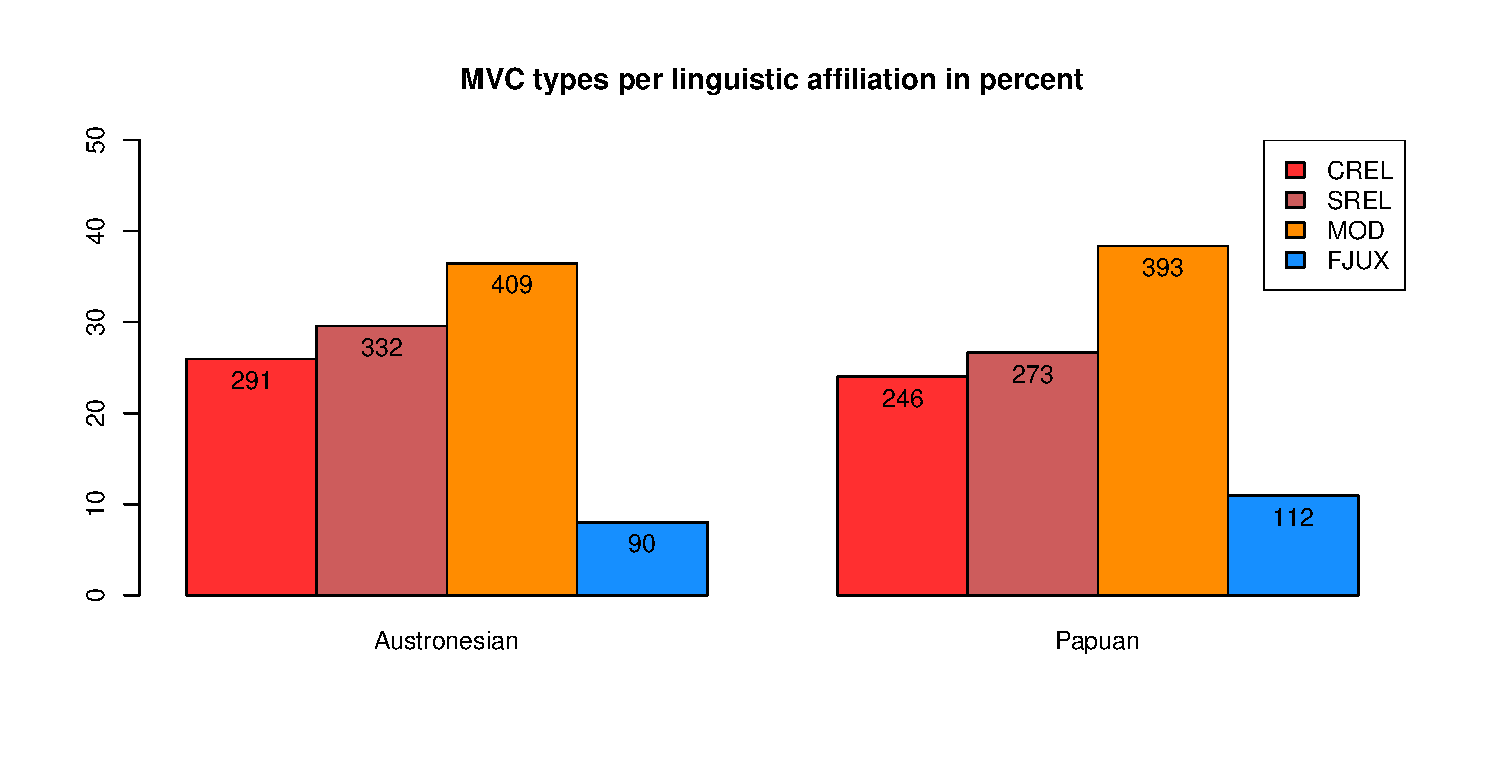
\includegraphics[width=\columnwidth]{figures/Type_Family.eps}
\caption[MVC types per linguistic affiliation in percent]{MVC types per linguistic affiliation in percent. CREL = component-relating constructions, SREL = stage-relating constructions, MOD = modifying constructions, FJUX = free juxtaposition constructions. Numbers on top of the bars refer to the number of observations.}\label{fig:type-family}
\end{figure}
\begin{figure}
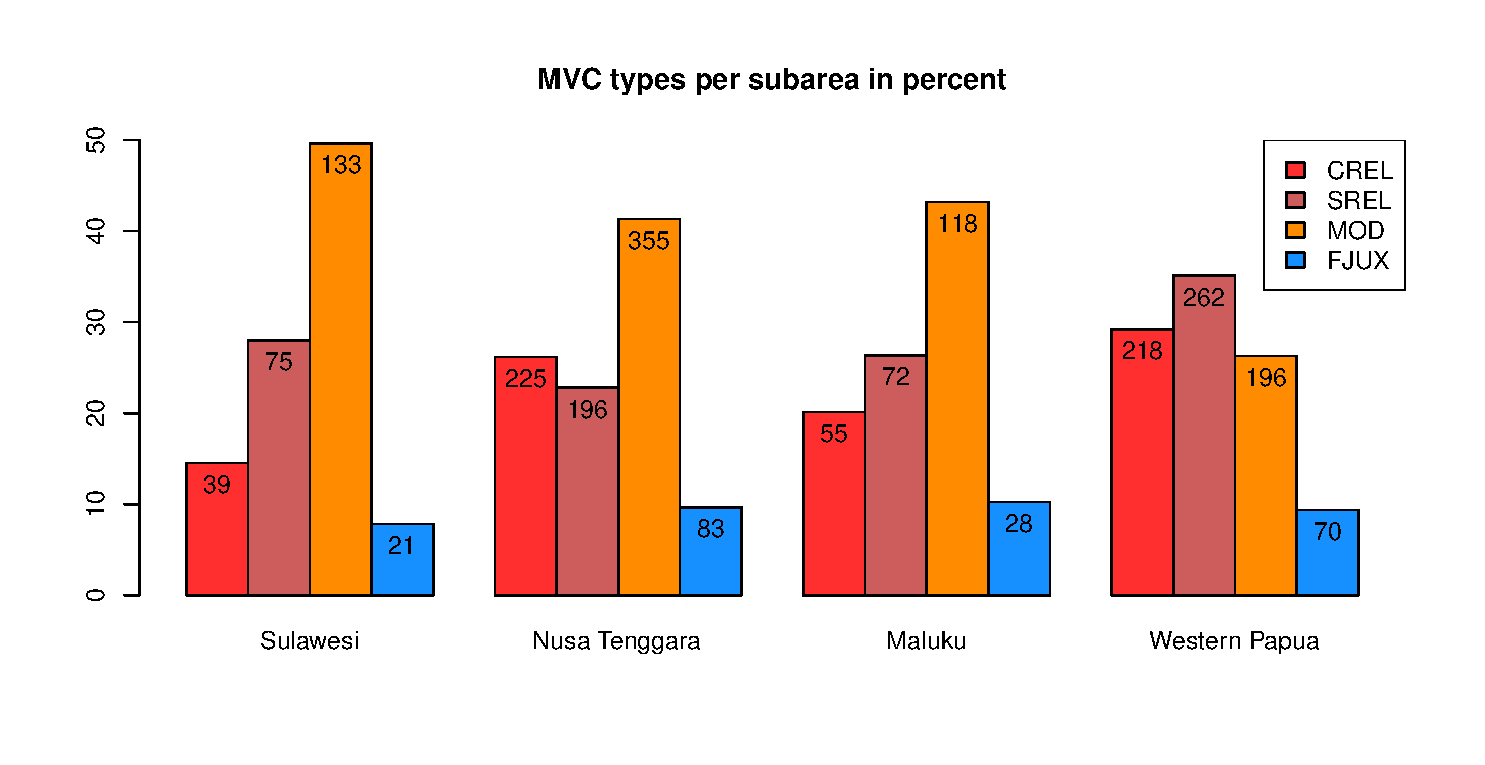
\includegraphics[width=\columnwidth]{figures/Type_Group.eps}
\caption[MVC types per subarea in percent]{MVC types per subarea in percent. CREL = component-relating constructions, SREL = stage-relating constructions, MOD = modifying constructions, FJUX = free juxtaposition constructions. Numbers on top of the bars refer to the number of observations.}\label{fig:type-group6}
\end{figure}

The general trend from \figref{fig:type-family} is mirrored in \figref{fig:type-group6} on MVC types per subarea, though the ratio is subject to some variation between the subareas. If we just focus on the three western subareas (\textsc{sul}, \textsc{nus}, and \textsc{mal}), a prevalence of modifying constructions is observable, with a peak of almost 50\% in the Sulawesi group. This seems suprising, given that the most prototypical modifying MVCs need to result from a considerable time span of grammaticalisation (think for instance of case-marking MVCs such as `give'/`for', `take'/`with' and so on). Thus it would appear that Sulawesi as a subarea is not peripheral in terms of feature innovation. However, as \tabref{table:MVCperlang} reveals, the geographically peripheral status of Sulawesi seems to be confirmed by the per language data, as there is a sharp split between the northern group (Pendau and Tajio) and the south-eastern group (Tolaki, Muna, and Tukang Besi). It is only in the latter group that modifying constructions score highest. Both Pendau and Tajio have MOD constructions to a much lesser extent, with motion constructions from the CREL and SREL families prevailing instead. The south-eastern languages, on the other hand, only exhibit weak signs of CREL use.

The Western Papua group deviates furthest from the overall MVC type ratio. Modifying constructions are less preferred than both CRELs and SRELs. Stage-relating constructions are particularly well-attested, with about 35\% of all instances. What remains stable across all four subgroups is the low percentage of recorded FJUX constructions.

\begin{table}
\begin{footnotesize}
\begin{tabular}{lrrrr}
  \lsptoprule
 & CREL & SREL & MOD & FJUX \\ 
  \midrule
  Muna &   6 &   2 &  32  &   10  \\ 
  Pendau &  26 &  19 &   5  &   1  \\ 
  Tajio &   4 &  18 &   6  &   4  \\ 
  Tolaki &   3 &  20 &  40  &   2  \\ 
  Tukang Besi &   0 &  16 &  50   &   4 \\ \midrule 
  Abui &  10 &  20 &  73  &   6  \\ 
  Alorese &  23 &  17 &   4  &   3  \\ 
  Bunaq &  23 &   6 &  55  &   3  \\ 
  Kaera &  9 &   10 &  4  &   1  \\ 
  Kambera &  15 &   2 &  24  &   3  \\ 
  Klon &  28 &  25 &  40  &   7  \\ 
  Makalero &  17 &   9 &  48  &   2  \\ 
  Teiwa &   18 &  29 &  17  &   21  \\ 
  Tetun &  25 &  19 &  26  &   3  \\ 
  Waima'a &  47 &  44 &  52  &  33  \\ 
  Western Pantar &  10 &  15 &  12  &   1  \\ \midrule
  Buru & 10 & 21 & 33 & 4 \\
  Selaru &   3 &   2 &   17  &   2  \\ 
  Taba &   2 &  18 &  22  &   2  \\ 
  Tidore & 33 & 23 & 23 & 13 \\
  Tobelo &   7 &   8 &  23  &   6  \\ \midrule
  Abun &  13 &  15 &   1  &   4  \\ 
  Biak &  18 &  31 &  16  &   2  \\ 
  Dusner &  18 &  17 &   9  &  5 \\ 
  Hatam &  18 &  23 &   6  &   2  \\ 
  Inanwatan &  11 &   6 &   4  &   7  \\ 
  Maybrat &  18 &  21 &  30  &   9  \\ 
  Mor &  35 &  23 &   7  &   6  \\ 
  Moskona &   5 &  30 &  38  &   6  \\ 
  Mpur &  15 &  14 &  16  &  17  \\ 
  Sougb &   11 &  19 &   3  &   7 \\ 
  Wooi &  56 &  63 &  66  &   5  \\ 
   \midrule
   Total & 537 & 605 & 802 & 202 \\
   \lspbottomrule
\end{tabular}
\end{footnotesize}
\caption[Distribution of attested MVC types per language]{Distribution of attested MVC types per language.}
\label{table:MVCperlang}
\end{table}

\tabref{table:MVCperlang} gives the numbers of MVC types per language. All languages seem to make use of all four constructional families, with the exception of Tukang Besi, for which no component-relating constructions could be found. Although all languages have reported instances of all construction types, different profiles are visible. Some languages, such as Abun or Alorese, show only very few cases of MODs. Other languages have few cases of CRELs (and, to a lesser extent, SRELs) but show a proliferation of MODs, like the group of south-eastern Sulawesi languages already mentioned. Still other languages, such as the two corpus languages Waima'a and Wooi, seem to make good use of all construction families (although FJUX scores very low in Wooi). 

Summing up, it is evident that all four techniques of MVC formation are in use all across EI. The factors that may explain the variation in the ratio of MVC types seen above will only become clear if we take a closer look at how the different constructions are distributed across the language sample. Therefore, I will turn to the four MVC families in the remainder of this chapter, providing examples of the different constructions that I assume to be associated with them, and exploring the patterns of use that can be unearthed from the data sample.

\section{Component-relating constructions}\label{sec:crel}

The notion \textit{component} here relates to verb strings in which each verb contributes part of the overall semantic structure of the MVC. This is meant to exclude other types of MVCs where the verbs do not enter into a merging relation, i.e. their LCS do not undergo a feature matching process. The term \textit{component} should therefore not be confused with other uses in the literature. For instance, \citet{dixon2006serial} seems to use the term \textit{component verb} to refer to any verb that takes part in a serialisation construction. Another conflicting use of the term is the distinction into component vs. narrative SVCs by \citet{vanstaden2008serial}. It is based upon the notion of \textit{macro event} introduced by \citet{talmy2000toward} and formally elaborated into a testable category by \citet{bohnemeyer2007principles, bohnemeyer2011}. A construction is said to be ``component-relating" when it ``compose[s] so-called `macro-events’
out of smaller units that we refer to as `subevents’", and it is called ``narrative" when it ``compose[s] larger event complexes out of macro events" \citep[28]{vanstaden2008serial}. Thus the definition of componentiality is essentially derived from an event-based account. 

Componential in my sense of the term only pertains to the features that are present in a set of related constructions throughout the EI languages, specifically these: (i) both (all) verbs belong to the same lexical field (which presupposes in my approach at least a partially identical make-up of LCS's), (ii) having a LCS that is (partially) identical, the verbs merge part of their features, (iii) if features are overwritten in the merging process, it is features of V$_{1}$ that are preserved and features of V$_{\textsc{fin}}$ that are overwritten. From the criteria previously discussed it has become clear that both CREL and MOD constructions appear to possess the macro-event property (MEP) as defined by \citet{bohnemeyer2007principles}. This is indicated by the fact that these construction types do not allow for partial temporal modification. Hence, while I motivate this constraint by assuming differences in the assignment of hidden event arguments, my understanding of \textit{component-relating} is quite similar to van Staden and Reesink's \textit{component SVCs}. Specifically, I share their insight that among serialisation constructions there are cases that are conceptually packed rather closely while other constructions have parts that behave more like independent subunits.

In the last chapter, I presented an approach to motivate merging of verbal features in a MVC by proposing a set of sublexical structures that might be shared. In order to enable structural merging between verbs of the same lexical field, I introduced empty class predicates \textbf{move'} for motion verbs and \textbf{say'} for speech act verbs. In principle, this approach could be extended to any combination of verbs from identical classes, but as far as I can see it is only motion and speech verbs that behave this way in the EI sample (with a handful of potential further combinations, see §\ref{sec:other}). 

In what follows, I will quickly preview the different CREL constructions found in the EI area, followed by a look at their distribution across the sample. The subsequent section will then introduce the respective constructions in more detail, and present examples from the sample. Motion CRELs appear in different construals. The most basic construal is motion complex MVCs, where a motion verb in V$_1$ (most typically a manner of motion verb) is complemented by a path or ground-denoting verb in V$_2$. This is the standard pattern of feature merging that I  proposed in §\ref{sec:merging} to be the underlying semantic process in CREL formation. Several related construals of complex motion seem to have been derived from this pattern. In \textsc{transport complex} MVCs, V$_1$ is a transitive verb of transport. In \textsc{direction complex} MVCs, V$_1$ is also transitive, but does not denote translational motion anymore. Rather, what is denoted is a movement verb to which V$_2$ adds path semantics. \textsc{Sequitive complex} MVCs have a \textsc{follow} verb in V$_1$. What all these constructions have in common is that some kind of \emph{movement} is involved, be it translational motion proper or movement of manipulated objects along some path.

Two more groups of CRELs are found in the EI region that are not related to movement. A \textsc{speech act complex} connects a speech act verb in V$_1$ to a \textsc{say} verb in V$_2$ introducing a propositional argument (what is said). The last group comprises some odd outliers that seem to involve feature merging yet are so infrequent throughout the sample that no distribution can be traced.

\begin{sidewaystable}
\begin{tabular}{lrrrr|rr}
  \lsptoprule
& \multicolumn{4}{c}{movement} & & \\
 & {motion} & {direction} & {transport} & {sequitive} & {speech act} & {other}\\  
  \midrule
  Austronesian & 166 & 46 & 47 & 9 & 20 & 3 \tabularnewline
  Papuan & 135 & 34 &  36 &  12 & 24 & 5 \tabularnewline
   \midrule
  Sulawesi & 25 & 8 & 6 & 0 & 0 & 0 \tabularnewline
  Nusa Tenggara & 144 & 35 & 22 & 7 & 10 & 7 \tabularnewline
  Maluku & 26 & 11 & 4 & 3 & 11 & 0 \tabularnewline 
  Papua & 106 & 26 & 51 & 11 & 23 & 1 \tabularnewline 
\midrule
Total & 301 & 83 & 80 & 21 & 44 & 8 \tabularnewline
\lspbottomrule
\end{tabular}
\caption[Distribution of CREL types]{Distribution of CREL types across EI. Note that both subcalculations, i.e. into language family affiliation as well as into areal subgroups, each amount to the total number of observations given in the last row.}
\label{table:CREL_overview}
\end{sidewaystable}

The impression from the previous section was that CREL constructions occur in almost all languages, and are evenly distributed over subareas and language families. If we look more closely at the different CREL constructions, this picture changes somewhat. \tabref{table:CREL_overview} above shows the distribution of CREL constructions across language families and subareas. The first thing to note is that CREL constructions involving movement figure most prominently: 485 out of 537 CREL observations involve movement of some kind. Among this group, motion complex constructions are most often attested, making it the default CREL construction in the EI sample. Figures \ref{fig:crel-family} and \ref{fig:crel-group} below illustrate the ratio between CREL constructions with regard to language affiliation and subgroup, respectively. Once more, we can discern that linguistic affiliation does not seem to bear on the use of the different constructions. It is only at the subarea level that we can observe considerable differences. The most obvious pattern is a lack of sequitive and speech act constructions in the Sulawesi subgroup. This tallies well with the assumption already mentioned that Sulawesi, forming the western periphery of an assumed Wallacea Sprachbund, does not have the full range of MVC constructions in use. The other three subareas each show all CREL constructions, although there are more observations of the minor constructions in Maluku and Western Papua languages than in the Nusa Tenggara languages.

\begin{figure}
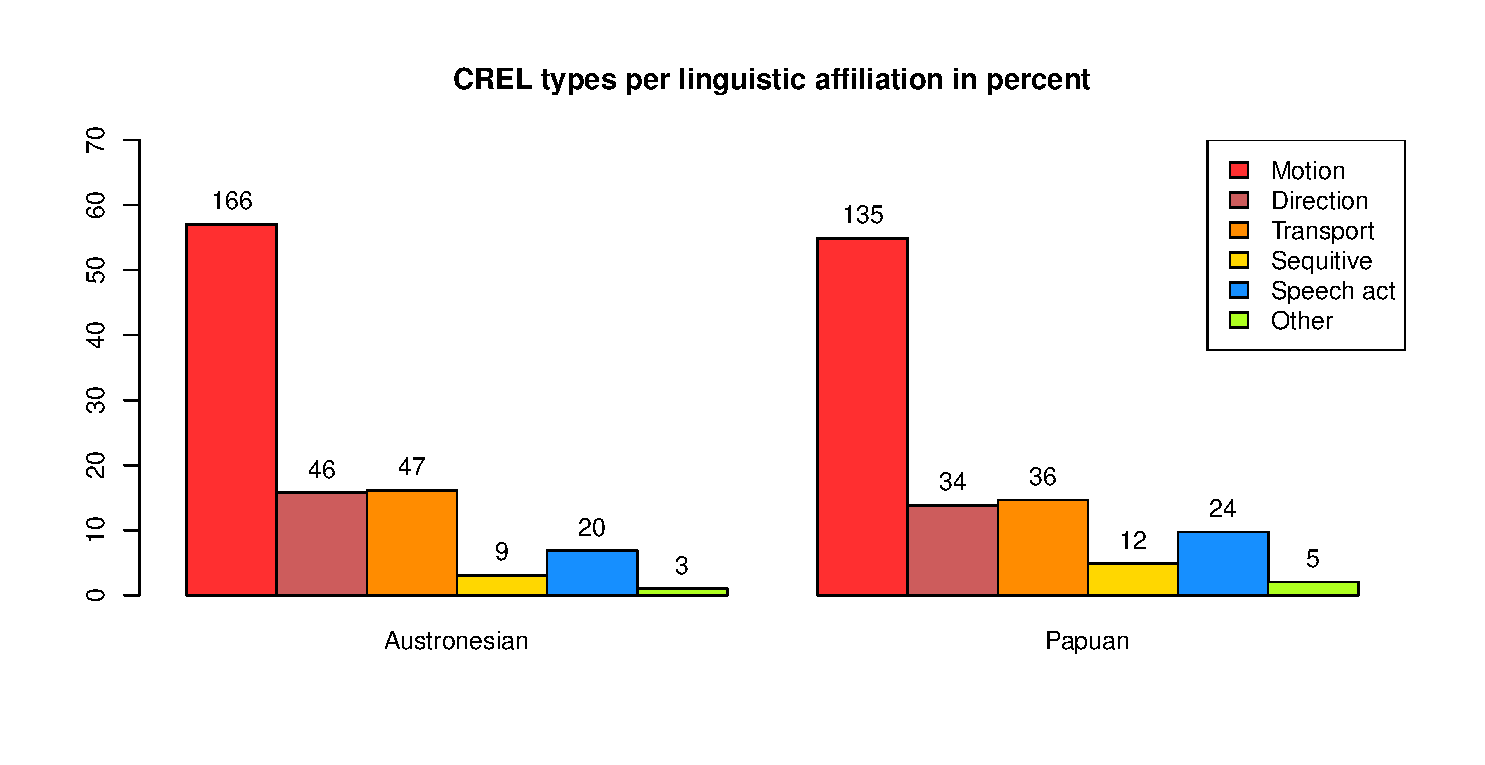
\includegraphics[width=\columnwidth]{figures/CREL_Family.eps}
\caption[CREL types per linguistic affiliation in percent]{CREL types per linguistic affiliation in percent. Numbers on top of the bars refer to the number of observations in the sample.}\label{fig:crel-family}
\end{figure}
\begin{figure}
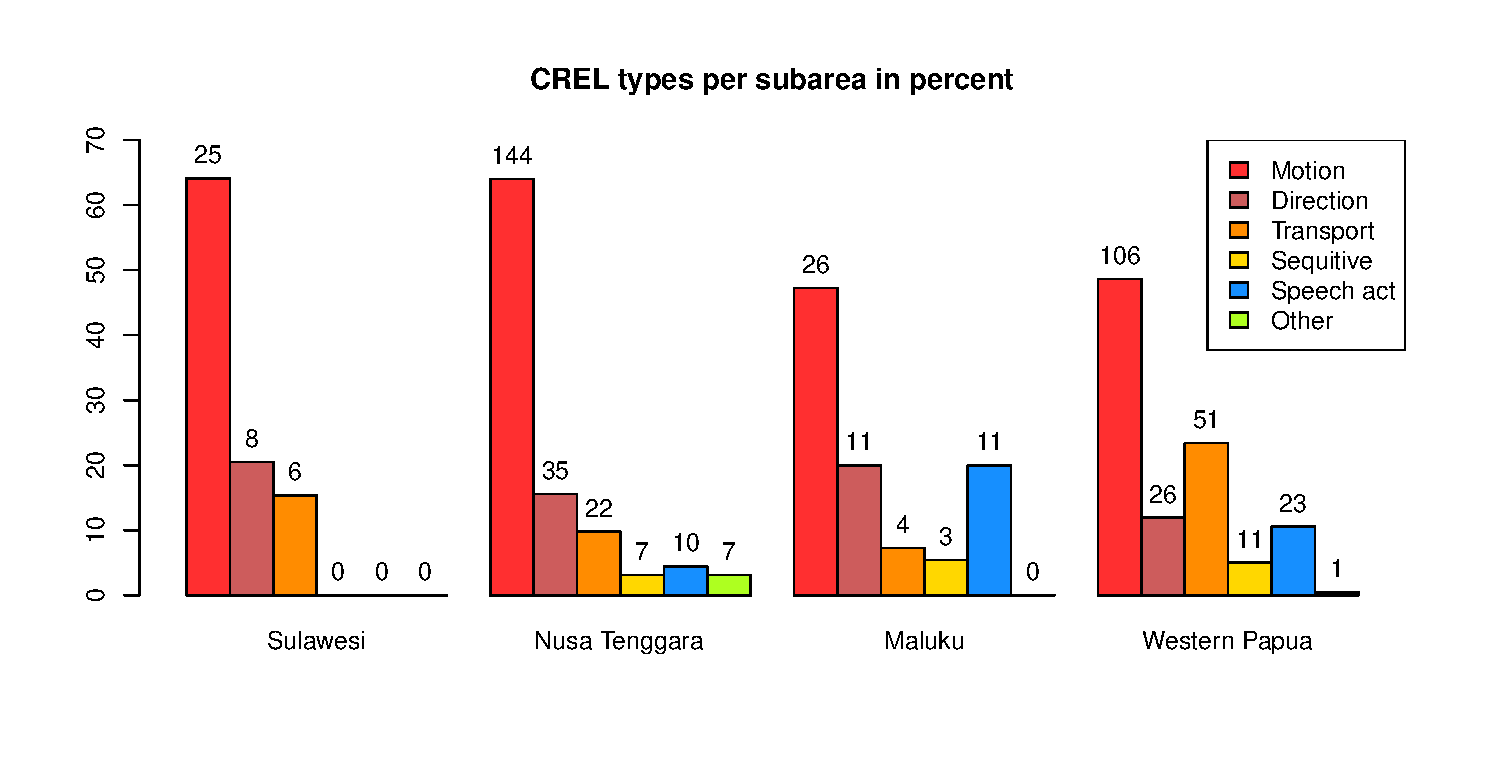
\includegraphics[width=\columnwidth]{figures/CREL_Group.eps}
\caption[CREL types per subarea in percent]{CREL types per subarea in percent. Numbers on top of the bars refer to the number of observations in the data sample.}\label{fig:crel-group}
\end{figure}

%\tabref{table:crel_language} below shows the distribution of attested CREL construction types per language. 

The different constructions are quite evenly distributed within the four subgroups. This shows that they are in fact widespread throughout the subareas, and do not just cluster in some exceptional language. If a language makes use of feature merging resulting in CRELs, there are always motion complex constructions among it. Direction, transport, and sequitive CRELs all involve transitive verbs in V$_1$ position, and the figures for these constructions are much lower than for motion complexes. What's more, the occurrence of the minor movement constructions appears to entail the use of the basic motion complex construction. That is, there are no languages for which only minor movement constructions are attested. This supports the assumption that the motion complex construction is the most basic one, possibly the construction from which the minor ones are derived. Another entailment suggested by the EI data is that if a language shows sequitive CRELs then it also tends to have attested direction and transport CRELs (with the exception of Inanwatan and Sougb). Direction and transport, on the other hand, seem not directly related to one another, as either construction may occur without the other.

%\begin{table}
%\begin{scriptsize}
%\begin{tabular}{lrrrrrr}
%\lsptoprule
%& \multicolumn{4}{c|}{movement} & & \\
% & {motion} & {direction} & {transport} & {sequitive} & {speech act} & {other}\\ 
 % \midrule
  %Muna &   5 &   0 &   1 &   0 &   0 &   0  \\ 
  %Pendau &  15 &   7 &   4 &   0 &   0 &   0 \\ 
  %Tajio &   3 &   0 &   1 &   0 &   0 &   0 \\ 
  %Tolaki &   2 &   1 &   0 &   0 &   0 &   0 \\ 
  %Tukang Besi & 0 & 0 & 0 & 0 & 0 & 0 \\ \midrule
  %Abui &   4 &   3 &   1 &   2 &   0 &   0 \\ 
  %Alorese &  19 &   1 &   1 &   1 &   1 &   0 \\ %
 % Bunaq &  18 &   5 &   0 &   0 &   0 &   0 \\ 
 % Kaera &   7 &   0 &   2 &   0 &   0 &   0 \\ 
 % Kambera &   3 &   4 &   4 &   1 &   1 &   2 \\ %
  %Klon &  21 &   0 &   0 &   0 &   4 &   3 \\ 
  %Makalero &  11 &   1 &   4 &   0 &   1 & 0  \\ %
  %Teiwa &   14 &   0 &   4 &   0 &   0 &   0 \\ 
  %Tetun &  16 &   4 &   4 &   0 &   0 &   1 \\ 
  %Waima'a &  23 &  17 &   2 &   3 &   2 &   0 \\ %
  %Western Pantar &   8 &   0 &   0 &   0 &   1 &   1 \\ \midrule
  %Buru & 8 & 1 & 0 & 0 & 1 & 0 \\
  %Selaru &   1 &   0 &   0 &   0 &   2 &   0 \\ 
  %Taba &   2 &   0 &   0 &   0 &   0 &   0 \\ 
  %Tidore & 13 & 9 & 4 & 3 & 4 & 0 \\
  %Tobelo &   2 &   1 &   0 &   0 &   4 &   0 \\ \midrule
 % Abun &   4 &   3 &   6 &   0 &   0 &   0 \\ 
 % Biak &   9 &   3 &   5 &   1 &   0 &   0 \\ 
 % Dusner &  11 &   0 &   4 &   1 &   2 &   0 \\ 
 % Hatam &   5 &   4 &   9 &   0 &   0 &   0 \\ 
 % Inanwatan &   4 &   0 &   4 &   2 &   0 &   1 \\ 
 % Maybrat &   8 &   4 &   0 &   0 &   6 &   0 \\ %
 % Mor &  15 &   2 &   8 &   2 &   8 &   0 \\ 
 % Moskona &   4 &   0 &   1 &   0 &   0 &   0 \\ %
 % Mpur &   4 &   4 &   0 &   5 &   2 &   0 \\ 
 % Sougb &   8 &   0 &   1 &   0 &   2 &   0 \\ 
 % Wooi &  34 &   6 &  13 &   0 &   3 &   0 \\ 
 %  \midrule
 %  Total & 301 & 80 & 83 & 21 & 44 & 8 \\
 %  \midrule
%\end{tabular}
%\end{scriptsize}
%\caption{Distribution of attested CREL construction types per language}
%\label{table:crel_language}
%\end{table}

Now, having arrived at a MVC analysis driven by semantic interaction techniques as introduced in Chapter \ref{ch:sem}, we can bring the morphosyntactic parameters from Chapter \ref{ch:gram} back into play. \tabref{table:crel_formal} illustrates that the CREL constructions display a much more homogeneous picture with regard to morphosyntactic properties than has been found for the whole sample in Chapter \ref{ch:gram}. In terms of referentiality, the same-subject configuration is strongly prevalent in all CREL constructions, except for direction complexes. This does not come as a surprise, given that in direction complexes, there is typically an argument-switch involved (see discussion below in §\ref{sec:direction}). This variation in referentiality encoding correlates with a tendency of direction complexes (as well as the other movement constructions) towards inflecting only the starting verb of the series. Uninflected V$_2$ in direction complexes thus leads to some degree of coding ambiguity with regard to argument interaction. This helps explain the wide range of referentiality values annotated.

The headedness patterns from \tabref{table:crel_formal} point out another notable tendency. In all movement constructions it is V$_1$ that is allocated the main inflectional load. The ``1" (first verb inflected) pattern is predominant across the board, and outnumbers the ``B" (both verbs inflected) pattern. Associating information on verbal categories, such as TAM or subject indexing, to only one head creates an asymmetry that can be interpreted as lending prominence to V$_1$. This is basically in line with the criterion introduced in §\ref{sec:criteria_mvcs} above, namely that in CREL it is V$_1$ that preserves its verbal properties rather than the subsequent verbs.\footnote{Note that these figures are slightly biased towards the ``1" pattern as I interpreted directional verboids in post-verbal position as verbs, for instance in languages that I am familiar with (Wooi, Waima'a) or where the lexeme in question can either diachronically or synchronically be traced back to a verb root (think of Wooi \textit{ma} from the very first example in Chapter \ref{ch:introduction}). Alternative analyses might reanalyse some such strings into verb - (directional) particle constructions, and arrive at lower numbers of ``1" patterns.} This prominence shift is, however, not visible in speech complex constructions, as these appear to favour the ``B" pattern.

\begin{table}
\centering
\begin{tabular}{rrrrrr}
  \lsptoprule
Referentiality & S & SO & D & A & E \\ 
  \midrule
motion complex & 300 &   0 &   0 &   0 &   1 \\ 
  direction complex &  20 &   5 &  33 &   0 &  22 \\ 
  transport complex &  80 &   0 &   2 &   1 &   0 \\ 
  sequitive complex &  19 &   0 &   2 &   0 &   0 \\ 
  speech act complex &  44 &   0 &   0 &   0 &   0 \\ 
  other &   8 &   0 &   0 &   0 &   0 \\ 
   \midrule
 \\
  \midrule
Headedness & B & 1 & 2 & S & N \\ 
  \midrule
motion complex &  39 &  83 &   2 &  10 &  14 \\ 
  direction complex &  12 &  22 &   0 &   5 &   6 \\ 
  transport complex &  15 &  32 &   4 &   4 &   4 \\ 
  sequitive complex &   3 &   6 &   2 &   2 &   2 \\ 
  speech act complex &  24 &   4 &   1 &   1 &   4 \\ 
  other &   0 &   0 &   1 &   2 &   0 \\ 
   \midrule
 \\
  \midrule
Contiguity & W & C & 1 & 2 & 3 \\ 
  \midrule
motion complex &   8 & 241 &  46 &   5 &   1 \\ 
  direction complex &   0 &  54 &  24 &   2 &   0 \\ 
  transport complex &   4 &  47 &  31 &   0 &   1 \\ 
  sequitive complex &   2 &  17 &   2 &   0 &   0 \\ 
  speech act complex &   0 &  34 &  10 &   0 &   0 \\ 
  other &   1 &   7 &   0 &   0 &   0 \\ 
   \lspbottomrule
\end{tabular}
\caption[Morphosyntactic properties of CREL constructions]{Morphosyntactic properties of CREL constructions in EI. Table components from top to bottom refer to referentiality (see §\ref{sec:argumentstructure}), headedness (see \ref{sec:headedness}), and contiguity (see \ref{sec:contiguity}), respectively. Referentiality values: S = Co-functional (``same subject"), SO = Transitive co-functional (``same subject and object"), D = Switch-function (``Different subject"), A = Participant accumulation, E = Event-to-argument (``Ambient"), X = no interaction, no arguments shared. Headedness values: B = Both verbs marked, 1 = First verb marked, 2 = Second/final verb marked, S = Shared affix set, N = None of the verbs marked. Contiguity values: W = Within word, C = Contiguous verbs 1 = One non-verbal constituent intervening, 2 = Two non-verbal constituents intervening, 3 = Three non-verbal constituents intervening, 4 = Four non-verbal constituents intervening.}
\label{table:crel_formal}
\end{table}

In the following sections, I will briefly present the CREL constructions one by one. The purpose of these sections is to provide examples from all subareas where the construction is attested.

\subsection{Motion complex} \label{sec:motioncomplex}

Motion complex constructions form the largest subgroup of the CREL class with 301 attested data points out of 537 instances of CRELs and 2146 instances of MVCs in total. The basic distributional properties are the same as for CRELs in general, since every language in the sample that has CREL constructions also has motion complexes. \tabref{table:basiccrelmotion} gives the respective numbers as well as the general template. A motion complex is made up of two or more verbs, with each verb belonging to the lexical field of motion verbs.

\begin{table}
\begin{tabular}{ll}
\lsptoprule
Feature&Value\tabularnewline
\midrule
Template&V1 \textsc{motion} -- V2 \textsc{motion}\tabularnewline
No. of attested instances& 301/2146 \tabularnewline
No. of attested languages& 31/32 (not attested: Tukang Besi) \tabularnewline
Distribution across areas& \textsc{sul} (4/5), \textsc{nus} (11/11), \textsc{mal} (5/5), \textsc{pap} (11/11) \tabularnewline
Distribution across families& \textsc{pap} (16), \textsc{aus} (15) \tabularnewline
\lspbottomrule
\end{tabular}
\caption[Template and basic distribution of CREL motion complexes]{Template and basic distribution of CREL motion complexes in the EI sample. First verb mostly intransitive with few exceptions, second verb intransitive or transitive}
\label{table:basiccrelmotion}
\end{table}

The following examples (\ref{Pendau24}) -- (\ref{Hatam001}) are from all four subareas, and show the typical appearance of motion complexes in EI. The first verb tends to be intransitive (with only a handful of exceptions, for instance \textsc{leave}, \textsc{cross}, or \textsc{reach} verbs taking a ground argument) and often refers to the way the motion is carried out, or gives part of the path information needed to project the whole motion vector. The verb in V$_{\textsc{fin}}$ is most often a path verb. In the Pendau example (\ref{Pendau24}) the moving referent undergoes a non-volitional motion event on a vertical projection plane. Example (\ref{Alorese001}) from Alorese shows a manner of motion verb followed again by a path verb, this time opening up a deictic vector directed towards the speaker origo. This example is somewhat unusual in that the moving referent is inanimate (most cases have animate actors performing some motion at will). Example (\ref{Taba002}) from Taba has another common combination of motion verbs with a reverse path verb in V$_{2}$ position and a vertical path verb in V$_{1}$. Note that the sample also contains motion complexes with exactly the opposite order, where a \textsc{return} verb is followed by a vertical or horizontal path verb. These cases are, however, restricted to combinations of motion verbs that both convey path semantics. Non-path-denoting motion verbs never appear in V$_1$, supporting the assumption that manner is placed before path in a motion complex. Example (\ref{Hatam001}) from Hatam has a potentially transitive ground-denoting verb in V$_{1}$ which, however, need not be produced with a ground NP. In cases like (\ref{Hatam001}), I interpret the function of contained path verbs (\textsc{enter}, \textsc{exit}) as emphasising additional information on the path, rather than introducing a ground referent which is not overtly specified.

\ea \label{Pendau24}
\langinfo{Pendau}{Austronesian, WMP}{\citealt[344]{Quick2007}}\\
\glll odo moo nanabumo manyau rilalong nuapi \\
odo moo no-nabu=mo ma-nyau ri=lalong nu=api \\
monkey this \textsc{st}.\textsc{rls}-fall=\textsc{compl} \textsc{irr}-go.down \textsc{loc}=inside \textsc{cn}=fire \\
\glft `This monkey fell down into the fire.' \\ 
\z

\ea \label{Alorese001}
\langinfo{Alorese}{Austronesian, CMP}{\citealt[63]{klamer2011alorese}}\\
\gll terus, kaju fatang nepi mene \\
then wood sea float come \\
\glft `Then a piece of wood came floating (towards us).'\\ 
\z

\ea \label{Taba002}
\langinfo{Taba}{Austronesian, SHWNG}{\citealt[295]{bowden2001taba}}\\
\glll ncopang nmul hu \\
n=sopang n=mul hu \\
\textsc{3}\textsc{sg}=descend \textsc{3}\textsc{sg}=return \textsc{cont} \\
\glft `(S)he's still coming back down.'\\ 
\z

\ea \label{Hatam001}
\langinfo{Hatam}{Papuan, Hatam-Mansim}{\citealt[100]{reesink1999grammar}}\\
\gll a-coi kwei \\
\textsc{2}\textsc{sg}-enter come \\
\glft `Come in.' (= invitation to visitor)\\ 
\z

The four examples are also typical motion complexes in terms of their morphosyntactic behaviour, as we have already seen from \tabref{table:crel_formal}. CREL motion complexes can basically appear in all inflection patterns. This is reflected by the examples: in (\ref{Pendau24}) and (\ref{Taba002}), both verbs take inflectional marking, example (\ref{Hatam001}) shows inflection only on the first verb, and in Alorese (\ref{Alorese001}) both verbs remain bare.\footnote{The Sulawesi case is a bit more complex inasmuch as a small group of motion verbs in V$_{\textsc{fin}}$ shows defective inflectional behaviour. In Pendau, only \textit{nyau} can occur with a prefix, either taking the form \textit{ma-nyau} or \textit{menyau} (from \textit{M-pe-nyau} \textsc{irr}-\textsc{sf/dyn}-go.down; see ex. (55) in \citealt[342]{Quick2007} and discussion on p.344 incl. footnote 8). As Quick's examples and discussion show, there is no realis form that would match \textsc{irr} \textit{ma-nyau}. A similar form occurs in neighbouring Tajio with \textit{minyau}, which could be analysed as a lexicalised former irrealis form. However, contemporary Tajio also lacks a realis counterpart (see \citealt[136]{mayani2013grammar}).} The choice of inflection pattern is probably influenced by two factors: (i) the overall grammatical system of the language, and (ii) dominance of the first verb. The second factor seems to be widespread in the EI area, and draws supportive evidence from two facts. First, as noted earlier, in feature merging it is features of V1 that are preserved (\textsc{fall} in V$_{1}$ passes on features of non-volitionality while \textsc{fall} in V$_{\textsc{fin}}$ does not). Second, the diachronic development in motion verb construals seems to suggest a gradual decline of verbal properties in V$_{\textsc{fin}}$, leading to the eventual loss of inflection and the ultimate formation of a class of directional operators. This process is well-known from many languages (see for instance \citealt[31]{Aikhenvald2006}).

Inanwatan is the only language in the sample that really seems to have developed a motion construction in which the second verb bears the morphosyntactic locus. Consider the following two examples.

\ea \label{Inanwatan16}
\langinfo{Inanwatan}{Papuan, SBH}{\citealt[49]{devries2004}}\\
\gll mé-se-i ewáiwa nóe-we-i-di \\
\textsc{3}\textsc{sbj}-walk-\textsc{pst}.\textsc{m} and go.out-\textsc{3}\textsc{sbj}-descend-\textsc{pst}.\textsc{m} \\
\glft `(And) he went on and on and he arrived.'\\ 
\z

\ea \label{Inanwatan20}
\langinfo{Inanwatan}{Papuan, SBH}{\citealt[55f.]{devries2004}}\\
\gll mé-de-wo-i ewáiwa \\
\textsc{3}\textsc{sbj}-go.across-come-\textsc{pst}.\textsc{sg}.\textsc{m} and \\
\glft `He came across and [...]'\\ 
\z

Example (\ref{Inanwatan16}) depicts the construction that I coded as ``2": the first motion verb, \textit{noé} `go out', is preposed to the finite verb complex, \textit{we-i-di} `he descended', as a bare stem. Another pattern, where both verbs share the inflection set of prefix and suffix, is illustrated in (\ref{Inanwatan20}). Here, both motion verbs can be conceived as inflected (\textit{shared inflection }in my terms). The fact that Inanwatan affords two different construals of motion complexes could indicate that the deictic path-denoting verb \textit{wo} `come' has already begun to lose part of its verbal properties in this context, moving along a grammaticalisation path that ultimately leads to the formation of a class of non-verbal directional elements. Inanwatan \textit{wo} would thus generally fit into the pattern of deverbalisation of \textsc{go} and \textsc{come} verbs in many EI languages.

Two languages in the \textsc{pap} subarea, Inanwatan and Sougb, allow motion complex construals within one phonological word. The Inanwatan examples (\ref{Inanwatan16}) and (\ref{Inanwatan20}) have already illustrated this type, and the figures for Inanwatan indicate that the construction pattern seems to be the only choice for motion complex construals in that language. Sougb is a bit different as it belongs to the group of languages with more than one attested contiguity value. The reason for this is that Sougb \textit{da} (from \textit{eda} `go') and \textit{in} (from \textit{en} `come'), the only two motion verbs attested in V$_{\textsc{fin}}$, behave like clitics: they attach to V$_{1}$, unless a direct object NP or a goal NP intervenes, in which case they attach to the NP. Note, however, that the source PP in (\ref{Sougb002a}) does not attract the clitic verb. The Sougb case is illustrated by the following examples:

\ea \label{Sougb002a}
\langinfo{Sougb}{Papuan, EBH}{\citealt[200]{reesink2002grammar}}\\
\gll godeh hom g-ougb-da dau m-ena \\
child one \textsc{nom}-run-go from \textsc{3}\textsc{sg}-father \\
\glft `A son who ran away from his father.' \\ 
\z

\ea
\langinfo{Sougb}{Papuan, EBH}{\citealt[226]{reesink2002grammar}}\\
\gll yen y-aiga duhu-da \\ 
you \textsc{2}\textsc{pl}-cross water-go \\
\glft `Cross the river.'\\ 
\z

\ea
\langinfo{Sougb}{Papuan, EBH}{\citealt[226]{reesink2002grammar}}\\
\gll en esogw-esa se duhu aud en-da \\ 
he jump-stand at water to him-go \\
\glft `He jumped into the water towards him.'\\ 
\z
\xe

Referentiality in motion complexes remains ``S" throughout all cases, as shown in \tabref{table:crel_formal} above. In principle, it is not clear why there are no languages that use the predicate-argument reanalysis scenario instead (in which the modifier verb takes the whole main verb predication as its argument). This pattern occurs in Southeast Sulawesi languages with construals of temporal verboids. If a temporal verboid, as shown in example (\ref{Muna018}) from Muna, can take as its subject the second VP, one might wonder why this is not also an option in motion complex MVCs, especially if the second verb is a path verb that has already lost part of its verbal properties. A construal like `it is usual (that) I swim' could then be paralleled by construals such as `it is hither I go/my going is hither'. Yet no such option is attested in the sample, except for one construction in Mpur, illustrated in (\ref{Mpur061}) .

\ea \label{Muna018}
\langinfo{Muna}{Austronesian, WMP}{\citealt[236f.]{vandenberg1989}}\\
\gll no-rea a-leni \\
\textsc{3}\textsc{sg}.\textsc{rls}-usual \textsc{1}\textsc{sg}.\textsc{rls}-swim \\
\glft `I usually swim.'\\ 
\z

\ea \label{Mpur061}
\langinfo{Mpur}{Papuan, isolate}{\citealt[101]{ode2002sketch}}\\
\gll bisa n-dokwa na n-aw a-ye' \\
can \textsc{1}\textsc{sg}-bring for \textsc{3}\textsc{sg}.\textsc{f}-run \textsc{3}\textsc{sg}.\textsc{m}-out \\
\glft `Bring (something) to get her out.'\\ 
\z

The motion complex \textit{n-aw a-ye'} here is construed as a purpose complement, marked as such by \textit{na}. Mpur has an overt gender distinction between masculine and feminine in third person singular. In (\ref{Mpur061}) we observe a mismatch in gender marking between the first verb and the second, indicating that the masculine subject of the outward movement denoted by \textit{ye'} cannot be the female runner from V$_{1}$. The only other interpretation that seems to be available here is that \textsc{3sg.m} can be used as a default marker for sentential arguments in Mpur, taking the first VP \textit{n-aw} as a subject here. Predicate-argument reanalysis is a feature that is further attested in the Bird's Head area, for instance in argument-marking constructions from Maybrat, in sequentialiser constructions from Moi (not part of the sample), or manner serialisation in Moskona, where the zero-marked manner verb is interpreted to take the entire predicate of the main verb as its subject \citep[299f.]{gravelle2010grammar}. 

Summarising so far, we have seen that, despite the large amount of data points from almost all EI languages, motion complexes are moulded into a fairly consistent form. From a formal perspective we can state that the verbs tend to stand adjacent to each other and display co-referential participant marking (``same subject"). If there is verbal inflection then it is the first verb that tends to receive it, except for the \textsc{nus} subarea where constructions (and languages) without clear inflection patterns predominate. From a semantic viewpoint, the stable factor is that the verbs all belong to the lexical field of motion verbs and merge part of their LCS. The majority of the constructions have the following order: V$_{1}$ refers to the act of moving (predominantly lexicalised manner of motion) while V$_{\textsc{fin}}$ contributes information on the way the motion event unfolds through space and time. Yet, we have already seen other examples (e.g. the Inanwatan examples in (\ref{Inanwatan16})) where V$_{1}$ presents path information and/or introduces (covert) ground referents (`go.out', `go.across'), which the motion event is set in relation to. This suggests that there is a good deal of variation as to which motion verb class appears in which constructional slot, in particular when language-specific constituent order constraints (as AOV in Inanwatan) clashes with the order dominant verb - modifier verb in motion complexes. The most crucial ordering principle, however, that I take to be at the heart of motion complex constructions, \textsc{manner} before \textsc{path}, is well-attested and not subject to any change in order. This constraint offers an interesting perspective on the framing discussion in complex motion expressions (as already briefly mentioned in §\ref{sec:sem-templates}). Talmy's two-way typology \citep{talmy1985lexicalization, talmy2000toward} has recently been expanded into a three-way typology, accomodating serialising languages as an independent framing type (called equipollently-framed by \citealt{slobin2004many}). While the nature of motion framing in SVCs is still under discussion, it is quite remarkable that both satellite-framed and serialising languages show a strong preference to place \textsc{manner} before \textsc{path} (see \citealt{Ameka2013} for a recent overview).

\subsection{Direction complex} \label{sec:direction}
Direction complexes bear a resemblance to motion complexes, as well as to transport complexes (see \ref{sec:transport}). With both construction types they share the (predominant) use of motion path verbs in V$_{\textsc{fin}}$ defining a trajectory of the motion event. Another feature they share with transport complexes is that the first verb in a direction complex is in most cases transitive (only directed perception verbs such as \textsc{look} deviate from this pattern). They differ, however, from both motion complexes and transport complexes in that the motion event is no longer understood as translational motion, but as a derived motion concept, capturing body part movement as well as stimulus perception vectors. \tabref{table:basiccreldir} has the basic features of direction complexes in the EI area.

\begin{table}
\begin{tabular}{ll}
\lsptoprule
Feature&Value\tabularnewline
\midrule
Template&V1 \textsc{action/perception$_{\textsc{tr}}$} - V2 \textsc{motion$_\textsc{intr}$}\tabularnewline
No. of attested instances& 80/2146 \tabularnewline
No. of attested languages& 19/32 \tabularnewline
Distribution across areas& \textsc{sul} (2/5), \textsc{nus} (7/11), \textsc{mal} (3/5), \textsc{pap} (7/11) \tabularnewline
Distribution across families& \textsc{pap} (9), \textsc{aus} (10) \tabularnewline
\lspbottomrule
\end{tabular}
\caption[Template and basic distribution of CREL direction complexes]{Template and basic distribution of CREL direction complexes in the EI data sample. First verb denotes object manipulation/relocation or perception, second verb contributes motion path semantics.}
\label{table:basiccreldir}
\end{table}


The following examples present typical cases of direction complexes from the \textsc{sul}, \textsc{nus}, and \textsc{pap} subareas (the only example from \textsc{mal} will be discussed further below). All three of them make use of a vertical or deictic path verb in V$_{\textsc{fin}}$, yet the event does not encode translational motion of the actor. In (\ref{Pendau027}) the path verb \textit{manyau} denotes a downward trajectory of some instrument. Pendau is the only \textsc{sul} language with several cases of attested direction complexes, both in combination with verbs of object manipulation (`cast', `slash') and with perception verbs (`stare', `look'). Example (\ref{Abui061}) from Abui illustrates a directed perception event, where the vertical path verb \textit{mara} adds the vector that spans between the experiencer (introduced here by grammaticalised \textit{ng} `see') and his visual focus. Again it is the constructional setting that pre-empts the motion verb from being interpreted as an act of literal motion. The last example is from the \textsc{pap} subarea and shows yet another way of combining an action verb with a motion path verb. \textit{tu} is a verb of object relocation rather than object manipulation, but serves well in a direction complex. Other examples from Maybrat involve the verb \textit{ai} `hit'.

\ea \label{Pendau027}
\langinfo{Pendau}{Austronesian, WMP}{\citealt[346]{Quick2007}}\\
\glll nitoto'a'onyo manyau riba'i nirapinyo \\
ni-toto'-a'=nyo ma-nyau ri=ba'i ni=rapi=nyo \\
\textsc{iv}.\textsc{rls}-slash-\textsc{tr}=\textsc{3}\textsc{sg}.\textsc{gen} \textsc{ug}.\textsc{irr}-go.down \textsc{loc}=head \textsc{pn}.\textsc{gen}=spouse=\textsc{3}\textsc{sg}.\textsc{gen} \\
\glft `He slashed it down into his wife's head.' \\ 
\z

\ea \label{Abui061}
\langinfo{Abui}{Papuan, TAP}{\citealt[363]{kratochvil2007grammar}}\\
\gll di=ng wahai mara \\
\textsc{3}\textsc{act}=see look go.up.\textsc{cont} \\
\glft ‘He looks up.’\\ 
\z
\xe

\ea \label{Maybrat102}
\langinfo{Maybrat}{Papuan, isolate}{\citealt[215]{dol2007grammar}}\\
\gll t-tu aya m-amo cerek a \\
\textsc{1}\textsc{sg}-pour water \textsc{3}\textsc{u}-go thermos.flask \textsc{q} \\
\glft `Should I pour water into the thermos flask?'\\ 
\z

The last example from Maybrat is reminiscent of ambient serialisation inasmuch as the referential alignment shows a mismatch between the subject of V$_{1}$ and V$_{\textsc{fin}}$. Dol explicitly discusses this construction as a shared argument construction and interprets the object of V$_{1}$ as subject of V$_{\textsc{fin}}$ \citep[217]{dol2007grammar}. That is, it is the water that `goes' into the thermos flask, not the pouring of the water as would be the case with ambient marking. 

One distributional property of direction complex constructions that is particularily striking is that all instances of direction complexes encoded as double-head inflection (``B" pattern) only feature verbs of object manipulation or relocation. There is not a single instance of double marking with perception constructions. This raises the following question: what is the (understood) subject of the motion path verb in V$_{\textsc{fin}}$? Is it the experiencer, the stimulus (with transitive perception verbs), the whole predication of perceiving something, or maybe none at all, as the motion verbs might have already lost part of their verbhood in that particular construction? An analysis of the EI sample shows that all languages that have both types (action and perception) attested either do not use verbal inflection at all (Alorese, Waima'a), or inflect the initial verb only (Biak, Wooi), or have irregular inflection patterns not generally suitable for characterising constructions (Pendau, Abui). Therefore we cannot at this point make any prediction regarding the identity of the second subject argument in direction complexes. Another feature that becomes evident is that all languages that allow for perceptional direction complexes are Austronesian languages (except for the one example from Abui illustrated in (\ref{Abui061}) above). If this tendency were confirmed with more data, one could state that direction complexes of the perception type are more common in Austronesian than in Papuan languages.

A final example that I want to present here is the only direction complex one from Tobelo. 

\ea \label{Tobelo033}
\langinfo{Tobelo}{Papuan, NH}{\citealt[63]{holton2003tobelo}}\\
\gll t-a-ika t-i-tauru no-maoko la no-ma-tagi \\
\textsc{1}-\textsc{vf}-\textsc{all} \textsc{1}-\textsc{3}\textsc{m}-pull \textsc{2}-stand \textsc{conj} \textsc{2}-\textsc{refl}-walk \\
\glft `I pulled him up so that he could walk.' \\ 
\z

This example is unusual in at least two ways (ignoring the resultant phase denoted by the third verb \textit{no-maoko}): first, the order of the verbs is reversed (motion path verb \textit{ika} -- action verb \textit{tauru}), a pattern that we do not find in the other languages. And second, the motion path verb seems to be grammatical in nature rather than a full lexical item (capable of predicating a simplex predicate). Such instances at best constitute peripheral cases of direction complexes, if at all.

\subsection{Transport complex} \label{sec:transport}

The next subtype of CREL constructions consists of a verb of transport, such as \textsc{bring}, \textsc{hold}, \textsc{carry}, or \textsc{bear}, which is complemented by a motion path verb in V$_2$. The combination of verbs is interpreted as denoting an act of translational motion, where the actor is in possession of an object and relocates it by way of changing his/her position in the landscape of discourse. \tabref{table:basiccreltransport} lists the basic properties of transport complexes in the EI languages. 

\begin{table}
\begin{tabular}{ll}
\lsptoprule
Feature&Value\tabularnewline
\midrule
Template&V1 \textsc{transport$_{\textsc{tr}}$} * V2 \textsc{motion}\tabularnewline
No. of attested instances& 83/2146 \tabularnewline
No. of attested languages& 21/32 \tabularnewline
Distribution across areas& \textsc{sul} (3/5), \textsc{nus} (8/11), \textsc{mal} (1/5), \textsc{pap} (9/11) \tabularnewline
Distribution across families& \textsc{pap} (11), \textsc{aus} (10) \tabularnewline
\lspbottomrule
\end{tabular}
\caption[Template and basic distribution of CREL transport complexes]{Template and basic distribution of CREL transport complexes in the EI sample. The first verb encodes possession and motion, the second verb contributes further motion components (predominantly path). The asterisk indicates that the order transport - motion is reversed in a small number of constructions}
\label{table:basiccreltransport}
\end{table}

Here are some examples from different subareas. The first example in (\ref{Tajio023}) is from Sulawesi, showing a \textsc{bring} verb in V$_{1}$ followed by a deictic path verb. Example (\ref{Makalero089}) uses another strategy to encode a transport event: here it is the handling verb \textit{mei} `take' that denotes the translocation of the item in question (which is a group of people here, it seems). More typical for transport constructions would be inanimate referents such as the tobacco in (\ref{Tajio023}). And (\ref{Hatam066}) from Hatam shows yet another option by using a \textsc{hold} verb again combined with a deictic motion verb in V$_{\textsc{fin}}$.

\ea \label{Tajio023}
\langinfo{Tajio}{Austronesian, WMP}{\citealt[294]{mayani2013grammar}}\\
\gll vava minyei ba i ulu tabako=mu \\
bring go.here please \textsc{loc} first tobacco=\textsc{2}\textsc{sg}.\textsc{poss} \\
\glft ‘Give me first your tobacco, please.'\\ 
\z

\ea \label{Makalero089}
\langinfo{Makalero}{Papuan, TAP}{\citealt[206]{huber2011}}\\
\gll ...ain=isi hai mei ma’u \\
\textsc{quot}=\textsc{lnk}\textsc{2} \textsc{nsit} take come \\
\glft `[direct speech] So she brought
them.'\\ 
\z

\ea \label{Hatam066}
\langinfo{Hatam}{Papuan, Hatam-Mansim}{\citealt[109]{reesink1999grammar}}\\
\gll yoni i-krau munggwom kwei big \\
they \textsc{3}\textsc{pl}-hold child come not \\
\glft `They don't bring the child(ren).' (lit. `They don't hold the child(ren) hither') \\ 
\z

Let us consider the evidence that a transport verb plus a motion verb do form a CREL construction type (and do not form instances of staging proper, or even simply emerge via free juxtaposition). Two aspects are vital here. First, we need to show that these verbs really act as a construction (at least in some languages).\footnote{This is of course a non-trivial enterprise. One starting point would be to try and muster evidence that the string has a meaning to it that cannot be derived from its components alone (i.e., showing that it is non-compositional). With regard to \textsc{take} -- \textsc{motion} combinations, this could for instance involve the testing of partial negation. Two-stage construals should allow for the negation of the motion stage, or the stage of obtaining some object. Something like `not taking it he went off' would indicate a two-stage construal.} And second, it must be clear that cases like (\ref{Makalero089}) are not interpreted as staged events (`take and come') but that the whole event description consists of one indivisible temporal frame (`take hither'). The EI data indicate that these assumptions turn out to be true. Hatam specifically is a clear case with regard to the first question. Consider the examples below. In each case we get three verbs in a string: \textit{ttei kwei bam} `carry come roast'. In the first instance in (\ref{Hatamtrans1}) \textit{ttei} is used as a single verb in a simplex predicate. Both a falling intonation pattern on \textit{ttei} as well as a considerable pause following it indicate that the first verb is to be interpreted separately from the other two. In (\ref{Hatamtrans2}), on the other hand, \textit{ttei} seems to form a tight construction with both \textit{kwei} and \textit{bam}, while in (\ref{Hatamtrans3}) it is only \textit{ttei} and \textit{kwei} that appear to be construed together. The difference is with the inflection pattern: in (\ref{Hatamtrans2}) only \textit{ttei} receives inflection, in (\ref{Hatamtrans3}) it is \textit{ttei} and \textit{bam} that are inflected. Conjunctive \textit{ba} is of course a further signal in (\ref{Hatamtrans3}) that there must be a constructional boundary between \textit{kwei} and \textit{bam}.

\a \label{Hatamtrans1}
\langinfo{Hatam}{Papuan, Hatam-Mansim}{\citealt[100]{reesink1999grammar}}\\
\gll lene $\emptyset$-pilei hanyen bu lene $\emptyset$-nduk nyeni ba ni-ttei. Ba ni-kwei bam \\
then \textsc{3}\textsc{sg}-shoot return again then \textsc{3}\textsc{sg}-gather us and \textsc{1}\textsc{ex}-carry and \textsc{1}\textsc{ex}-come roast \\
\glft `Then he shot (pig) again and called us together and we carried (it). And we came and roasted (it).' \\
\z

\ea \label{Hatamtrans2}
\langinfo{Hatam}{Papuan, Hatam-Mansim}{\citealt[101]{reesink1999grammar}}\\
\gll lene $\emptyset$-nduk nyeni ni-ttei kwei bam \\ 
then \textsc{3}\textsc{sg}-gather us \textsc{1}\textsc{ex}-carry come roast \\
\glft `Then he gathered us we carried, came, roasted.' \\ 
\z

\ea \label{Hatamtrans3}
\langinfo{Hatam}{Papuan, Hatam-Mansim}{\citealt[101]{reesink1999grammar}}\\
\gll lene $\emptyset$-nduk nyeni ni-ttei kwei ba ni-bam \\ 
then \textsc{3}\textsc{sg}-gather us \textsc{1}\textsc{ex}-carry come and \textsc{1}\textsc{ex}-roast \\
\glft `Then he gathered us, we carried, came and we roasted.'\\ 
\z

The inflection patterns suggest that we have to deal with two different constructions in the Hatam examples above. First, a motion-to-action construction with an inflected motion verb in V$_{1}$, and an uninflected action verb in V$_{\textsc{fin}}$ (illustrated by the second clause \textit{ni-kwei bam} in (\ref{Hatamtrans1})). And second, a transport complex in (\ref{Hatamtrans3}) with an inflected transport verb in V$_{1}$ and an uninflected motion path verb in V$_{\textsc{fin}}$. I have argued at the outset of this chapter that one difference between CREL and SREL constructions is that the former may be embedded into the latter but not vice versa. This is, I propose, the case in example (\ref{Hatamtrans2}), where insertion of a transport complex into the motion slot of a motion-to-action SREL leads to a sequence of three verbs of which only the first one is inflected. Inflectional marking is thus not allocated to the first \emph{verb} but to the first \emph{constituent} filling the motion slot (which is \textit{ttei kwei}). It is this behaviour that supports the assumption that transport verb plus motion verb can indeed be characterised (at least in some languages) as forming a construction.

Proving the second aspect (that \textsc{take} \textsc{come} is construed/conceived as `take hither' rather than `take and come') is more complicated, and I can ony hint at two points here. The first one is a tendency, the second one a curiosity. Starting with the tendency, the subsample of transport complexes shows that there is a small trend towards inflecting only the first verb but not the second. This is basically the Hatam type, where lack of inflection on the motion path verb can be interpreted as a ranking (hierarchy) of constituents within the construction. Such signs of morphosyntactic integration could thus be used as evidence for cognitive integration (although this point is difficult to validate, of course). The inflection counts become even clearer if we sort out certain cases. For instance, Reesink cogently notes that in Hatam more general motion verbs in V$_{\textsc{fin}}$ do not obey the initial-inflection pattern, but receive their own inflectional marking as if normally juxtaposed. Consider the following examples.

\ea \label{Hatam018}
\langinfo{Hatam}{Papuan, Hatam-Mansim}{\citealt[100]{reesink1999grammar}}\\
\gll a-ttei mikwau dini a-mbut tut ba a-yai bak a-sut-bat-nya \\
\textsc{2}\textsc{sg}-carry meat this \textsc{2}\textsc{sg}-walk along and \textsc{2}\textsc{sg}-take to \textsc{2}\textsc{sg}-friend-\textsc{coll}-\textsc{pl} \\
\glft `Take this meat (and) go with (it) and give it to your friends.'\\ 
\z

In (\ref{Hatam018}) it is a manner of motion verb and not a path-denoting motion verb that follows \textit{ttei}, and consequently fails to fill the second slot of a (potential) transport complex (\textit{mbut} must inflect here, see \citealt[100]{reesink1999grammar}). This becomes predictable if we assume the second slot to permit only those verbs that under feature merging specify the spatial vector of the motion event. Transport complexes would thus parallel the bulk of motion complexes in that both construction types feature path specification in V$_{\textsc{fin}}$. 

In a similar vein, we could exclude deviating examples such as the following from Wooi.

\ea \label{Wooi137}
\langinfo{Wooi}{Austronesian, SHWNG}{soul\_child\_woods}\\
\glll hengko hnia henda to wirey \\
he-ko hnia he-ra to wirey \\
\textsc{3}\textsc{pl}-take them \textsc{3}\textsc{pl}-go \textsc{dir} forest \\
\glft `They take them (and) go to the forest.'\\ 
\z

A transport complex construction is very well attested in Wooi. Its pattern is similar to the Hatam case where the first verb takes inflection and the second verb does not. The motion verb in V$_{\textsc{fin}}$ belongs to a smallish group of three path verbs, \textit{ra} `go', \textit{ma} `come/hither' and \textit{taveri} `return'. Example (\ref{Wooi137}), however, is exceptional as the motion verb here also takes inflection, and thus seems to be an instance of staging rather than a construal of transport. This becomes clear when we take the subsequent utterance into account:

\ea \label{Wooi137add}
\langinfo{Wooi}{Austronesian, SHWNG}{soul\_child\_woods}\\
\glll hengko hnia $<$hen-$>$ retenenag henda to wirey ma \\
he-ko hnia he- retenang he-ra to wirey ma\\
\textsc{3}\textsc{pl}-take them $<$go-$>$ first \textsc{3}\textsc{pl}-go \textsc{dir} forest come \\
\glft `They take them -, first they go to the forest (with them).'\\
\z

In (\ref{Wooi137add}) the speaker is about to deliver the same collocation as in (\ref{Wooi137}) (\textit{hengko hnia henda}) but then aborts it and starts anew with a motion complex instead (\textit{henda ... ma}). If the handling verb and the motion verb indeed formed an underlying construction, standard assumptions on serialisation would expect the speaker to be forced to repeat the whole construction (*\textit{retenang hengko hnia henda ...}). This is, however, not the case. We might rather assume two juxtaposed verbs here of which the speaker is free to repeat only the second one. Note that this argument is identical to the opening argument in \citet{senft2008intro} where he observed that in cases of self repair Kilivila speakers repeat the whole verb string of a SVC and not just the part intended to be fixed. I am making this point here in order to show that not every collocation of transport verb and motion verb necessarily qualifies as a transport complex, even if the language in question does use this construction.

The second clue that might support the assumption of a semantically coherent event without temporal stages comes from a transport complex found in Moi, a West Papuan language not included in the EI sample. Moi also uses a \textsc{take} verb in V$_{1}$, as illustrated in (\ref{Moi001}).

\ea \label{Moi001}
\langinfo{Moi}{Papuan, WBH}{\citealt[51]{menick1996verb}}\\
\gll yi-sik kuwok p-ama \\
\textsc{3}\textsc{hum}-take stringbag \textsc{3}\textsc{nhum}-come \\
\glft `They took the stringbag here.'\\ 
\z

The curious thing about the Moi transport complex is the referential alignment pattern. Moi makes a distinction between human and non-human referents in the third person. This difference can be seen in (\ref{Moi001}) where the \textsc{take} verb inflects for 3\textsc{hum}, while the motion verb takes non-human marking. The subject of \textit{ama} `come' thus cannot be co-referential with the subject of \textit{sik}, and the group of human referents cannot be construed as the ones coming. The interpretation of \textit{p-ama} would therefore either have to assume subject agreement with the object of V$_{1}$, \textit{kuwok} the stringbag, or involve predicate-argument reanalysis where the motion verb takes the whole first VP \textit{yi-sik kuwok} as subject argument. Under either interpretation, it hardly seems plausible that each verb denotes a distinct temporal stage (\textsc{take} and then \textsc{come}) as the second verb would then have a non-human yet independently moving subject referent.

Semantic LCS merging between \textsc{carry} verbs and motion path verbs is straightforward inasmuch as both verbs have the motion predicate \textbf{move'} enabling LCS combination. This is most obvious in cases like (\ref{Tajio023}) from Tajio above where the glossing of the transport verb implies durative motion. The semantic relation between the verbs is less clear, however, if the transport verb belongs to the class of handling verbs, in particular \textsc{take} and \textsc{hold} verbs. In some grammars, the glossing of handling verbs alternates between `take' and `carry' (Abun), `hold' and `get' (Abui), or `take' and `use' (Hatam), highlighting the conceptual proximity between the punctual and non-punctual readings (recall the discussion in §\ref{sec:verbglossing}). Carrying an object presupposes its being taken up, and taking an object may well lead us to assume that what comes next could be its being carried somewhere. Such glossing alternations in fact show, I think, that two different semantic templates are available for these verbs. First, the lexeme might cover a punctual reading of object obtainment (manually coming into possession of x). This template does not necessarily involve translational motion and is used in collocations of object manipulation as in English \textit{take the toast and butter it}. In a similar vein, it is used in SREL MVCs of the type handling-to-action, to be discussed in §\ref{sec:handling-to-action} below. Second, there is a durative motion reading (manually coming into possession and translocation of x), where the temporal frame is more complex (and in the case of \textsc{hold} verbs the change-of-possession part may actually only be inferred by conventional implicature). This second template that in my proposal has a \textbf{move'} predicate is used in CREL transport complexes (just as in \textit{take the toast to the bathroom}). 

Direct evidence for this assumption comes from the fact that we rarely ever find handling-to-action constructions an uninflected action verb.\todo{rephrase}
In contrast, many transport complexes show deranking of the motion verb in V$_{\textsc{fin}}$ suggesting a gradual erosion of verbal properties. To this observation we can add another: a set of grammaticalised constructions in different languages shows that handling verbs (\textsc{take} and \textsc{hold)} may evolve into grammatical formatives. This seems to suggest the following general pattern: in transport complexes the motion verb in V$_{\textsc{fin}}$ tends to develop into a directional element whereas the handling verb remains stable. In handling-to-action constructions, the handling verb (initially residing in V$_{1}$, conditioned by strict temporal iconicity of event stages) is prone to undergo grammaticalisation clines of various kinds while the action/main verb in V$_{\textsc{fin}}$ remains stable. The EI sample bears witness to the following developments: in Maybrat, the \textsc{take} verb \textit{-o} has acquired a modality-like meaning in the construction \textit{-o} + \textsc{verb} meaning `really/truly \textsc{verb}ing' \citep[195]{dol2007grammar}. In Makalero, the \textsc{take} verb \textit{mei} has developed into a light verb, which provides an additional argument position in transitive or ditransitive clauses in cases where the main verb slots are already blocked by complements \citep[203]{huber2011}. And in Abui, \textsc{hold} verbs can express comitative arguments, participants attributed with a specific property, as well as narrow focus \citep[382--7]{kratochvil2007grammar}.

Some languages do not show signs of a lexicalised \textsc{carry} verb, so it might be the case that speakers in these languages prefer to construe the durative meaning by combining a \textsc{take} verb plus motion path verb. This is reminiscent of languages like Kalam, where MVCs are vastly productive in providing meaning combinations that are lexicalised in other languages \citep{pawley2011event}. 

\subsection{Sequitive complex} \label{sec:sequitive}

The last group of movement CRELs is less homogeneous than the others. The common feature in sequitive complexes is the use of a verb of following or pursuit, either in V$_{1}$ or V$_{\textsc{fin}}$. I decided to treat sequitive complexes separately early on because initial \textsc{follow} may evolve into an aspectual marker in some languages such as in Wooi, denoting the repetition of some previous action performed by other participants (essentially `also' semantics: \textit{follow} \textsc{verb} $>$ \textit{also} \textsc{verb}). Grammaticalisation of \textsc{follow} in V$_{1}$ somewhat weakens the claim that CRELs show a clear tendency for the \emph{final} verb to grammaticalise. Perhaps this indicates that sequitive constructions with \textsc{follow} in V$_{1}$ in fact are rather different from the other CREL types. For the time being, I leave all instances involving a \textsc{follow} verb together with another motion verb in this section, as there are only few data available. This means that both orders, \textsc{follow} -- motion verb, and motion verb -- \textsc{follow}, are at present collapsed into one category.

The second arrangement, i.e. with a \textsc{follow} verb in V$_{\textsc{fin}}$, behaves more like typical CRELs in that verbal inflection of \textsc{follow} is mostly lost. Here, \textsc{follow} looks rather like an ordinary path verb, and often lacks explicit infomation on the object or person followed. As can be seen from \tabref{table:basiccrelseq}, sequitive complexes only form a tiny fraction of attested MVCs making it hard to predict a uniform construction type (or two, for that matter) at this point.

\begin{table}
\begin{tabular}{ll}
\lsptoprule
Feature&Value\tabularnewline
\midrule
Template&V1 \textsc{follow$_{\textsc{tr}}$} * V2 \textsc{motion}\tabularnewline
No. of attested instances& 21/2146 \tabularnewline
No. of attested languages& 10/32 \tabularnewline
Distribution across areas& \textsc{nus} (4/11), \textsc{mal} (1/5), \textsc{pap} (5/11) \tabularnewline
Distribution across families& \textsc{pap} (4), \textsc{aus} (6) \tabularnewline
\lspbottomrule
\end{tabular}
\caption[Template and basic distribution of CREL sequitive complexes]{Template and basic distribution of CREL sequitive complexes in the EI sample. One verb is a \textsc{follow} verb (or related concept), the other is a motion verb, most often a manner verb. The asterisk indicates that both orders are found.}
\label{table:basiccrelseq}
\end{table}

Sequitive complexes are only attested with more than one language in the \textsc{nus} and \textsc{pap} subareas. The following examples start with the first subtype, namely \textsc{follow} - motion verb. This pattern is attested in Abui, Alorese, Mor, and Inanwatan. The first example from Abui illustrates a patient argument introduced by the verb \textit{luol} `gain' which, at least in this context, seems to have acquired a similar reading as a \textsc{follow} verb. A natural context for this utterance would be a situation where someone comes running up a hill, and then one of the bystanders is prompted to run up next \citep[362]{kratochvil2007grammar}. The next example is from Inanwatan. This is another instance of Inanwatan CREL constructions where the first verb is juxtaposed with a bare stem to the inflected second verb. Example (\ref{WBWHeri001}) shows an additional example from Wooi that I found when searching specifically for \textsc{follow} verbs in the Wooi corpus. It is therefore not part of the sample statistics. In the Wooi example, the object of following is a group of people indicated by the object marker \textit{-a}.

\ea \label{Abui059}
\langinfo{Abui}{Papuan, TAP}{\citealt[363]{kratochvil2007grammar}}\\
\gll ha-luol marang! \\
\textsc{3}\textsc{pat}-gain come.up \\
\glft `Follow it up!’, lit.: `Come up, gaining on it/him/them.’ \\ 
\z

\ea \label{Inanwatan026}
\langinfo{Inanwatan}{Papuan, SBH}{\citealt[59]{devries2004}}\\
\gll iyó míroqai-webe tigó áruqo qai-nigé-rowo-be \\
yes true-be it-be.\textsc{3}\textsc{sg}.\textsc{f} blood.\textsc{f} follow-\textsc{1}\textsc{pl}.\textsc{ex}.\textsc{sbj}-come.down-\textsc{prs} \\
\glft `Yes, that is true, we followed the bloodtrail.'\\ 
\z

\ea \label{WBWHeri001}
\langinfo{Wooi}{Austronesian, SHWNG}{space\_game4\_Heri 001}\\
\glll katu buonta taveri wipey e \\
katu bu-ong-a taveri wipey e \\
little.while \textsc{2}\textsc{sg}-follow-\textsc{obj}.\textsc{pl} return above \textsc{q} \\
\glft `Will you go back (with them) later?' \\ 
\z

Inanwatan shows another function of sequitive constructions. The theme argument of \textit{qai} in (\ref{Inanwatan026}) designates a route-like ground referent along which the motion event is projected. This function is also attested in Mor. In Wooi, \textit{ong} also combines with non-motion verbs and has in such environments developed adverbial semantics (also doing x). The bulk of Wooi examples are therefore interpreted as modifying constructions rather than as component-relating ones, as there is apparently no common subset of motion features that might be shared.

The second pattern motion verb - \textsc{follow} is found in Kambera, Waima'a, Biak, Dusner, Mor, and Mpur. Almost all cases have a motion verb in V$_{1}$ that denotes fast dynamic motion (\textsc{run}, \textsc{chase}, \textsc{rush} verbs). This is illustrated by the examples below. In languages like Mpur and Waima'a, the use of \textsc{run} + \textsc{follow} in fact looks like a frequent collocation and is possibly already on its way to becoming lexicalised.

\ea \label{Kambera003}
\langinfo{Kambera}{Austronesian, CMP}{\citealt[277]{klamer1998grammar}}\\
\gll na-palài nyara-ha da ahu la mbomang \\
\textsc{3}\textsc{sg}.\textsc{nom}-run chase-\textsc{3}\textsc{pl}.\textsc{acc} \textsc{art} dog \textsc{loc} space.under.house \\
\glft `He ran after the dogs under the house.' \\ 
\z

\ea \label{Biak005}
\langinfo{Biak}{Austronesian, SHWNG}{\citealt[183]{vanheuvel2006}}\\
\glll wamar ido, pon mura voi insape na yákyaw usr aw \\
wa-mar ido pon mu-ra voi insape na y-ák-yaw usr aw \\
\textsc{2}\textsc{sg}-die \textsc{top} \textsc{2}\textsc{sg}.first \textsc{path}-to.o.there but then then \textsc{1}\textsc{sg}-also-pursue follow \textsc{2}\textsc{sg} \\
\glft `When you die, you just go first to over there but later I will follow after you.'\\ 
\z

\ea 
\langinfo{Mpur}{Papuan, isolate}{\citealt[99]{ode2002sketch}}\\
\ea \label{Mpur057a}
\gll a-sit subwe-m \\
\textsc{3}\textsc{sg}.\textsc{m}-run after-\textsc{3}\textsc{sg}.\textsc{f} \\
\glft `He ran after her,' \\ 
\ex \label{Mpur057b}
\gll a-subwe-m n-aw n-aw n-aw n-aw n-aw n-aw n-aw n-aw n-aw n-aw \\
\textsc{3}\textsc{sg}.\textsc{m}-after-\textsc{3}\textsc{sg}.\textsc{f} \textsc{3}\textsc{sg}.\textsc{f}-run \textsc{3}\textsc{sg}.\textsc{f}-run \textsc{3}\textsc{sg}.\textsc{f}-run \textsc{3}\textsc{sg}.\textsc{f}-run \textsc{3}\textsc{sg}.\textsc{f}-run \textsc{3}\textsc{sg}.\textsc{f}-run \textsc{3}\textsc{sg}.\textsc{f}-run \textsc{3}\textsc{sg}.\textsc{f}-run \textsc{3}\textsc{sg}.\textsc{f}-run \textsc{3}\textsc{sg}.\textsc{f}-run\\
\glft `he followed her, she ran ran ran away.'\\ 
\z
\z

If we have a look at the morphosyntactic construal of motion - \textsc{follow} constructions we can detect signs of a de-ranked \textsc{follow} verb in V$_{\textsc{fin}}$. Iin Kambera, both verbs share a single set of agreement markers (\ref{Kambera003}). The same seems true for the Mpur case in (\ref{Mpur057a}) where \textit{subwe} takes object marking but no subject marking. A similar pattern has developed in Biak, where \textit{usr} no longer takes subject marking and fits into a group of postverbs \citep[183, and pp. 187--91]{vanheuvel2006}. Mpur is an interesting case as the subsequent utterance in (\ref{Mpur057b}) immediately shows the reverse pattern of (\ref{Mpur057a}) with the \textsc{follow} verb in front and the motion verb behind (repeated several times). As there is no indication of any prosodic disruption between the verbs (a feature that Odé carefully includes in her transcript) one would be tempted to assume a free order of constituents here if there had not been clear differences in construal: flipping \textit{subwe} into V$_{1}$ apparently changes its status, and requires full verbal inflection on both constituents. I do not present more details here as there is so little data, and I am not myself convinced that sequitive strings are indeed a recognisable CREL construction with sound cross-linguistic validity.

\subsection{Speech act complex} \label{sec:speechactcomplex}

The previous CREL types all made use of motion or movement verbs of different kinds. The following types  illustrate that other lexical fields are also used as resources for the formation of CRELs. I will start with speech complexes here as this is the only sizeable group that does not make use of the semantics of movement. A \textsc{speech act complex} consists of two speech act verbs, and thus draws from an entirely different source of verbs compared to the motion CRELs above. Yet both groups of CRELs share a common core: (1) as with motion CRELs, speech act complexes divide up the total amount of information on two (or more) independent lexemes; (2) speech complexes make use of verbs from the same lexical field, as motion CRELs do; (3) as with motion CRELs, it is the verb in V$_{\textsc{fin}}$ that in many cases appears to lose some of its verbal properties and becomes deranked in comparison to the main verb in V$_{1}$. \tabref{table:basiccrelspeech} starts with the basic numbers of the construction.

\begin{table}
\begin{tabular}{ll}
\lsptoprule
Feature&Value\tabularnewline
\midrule
Template&V1 \textsc{speech act verb} -- V2 \textsc{\textsc{say}}\tabularnewline
No. of attested instances& 44/2146 \tabularnewline
No. of attested languages& 16/32 \tabularnewline
Distribution across areas& \textsc{nus} (6/11), \textsc{mal} (4/5), \textsc{pap} (6/11) \tabularnewline
Distribution across families& \textsc{pap} (8), \textsc{aus} (8) \tabularnewline
\lspbottomrule
\end{tabular}
\caption[Template and basic distribution of CREL speech act complexes]{Template and basic distribution of CREL speech act complexes in the EI sample. The first verb belongs to the lexical field of speech act verbs, the second verb is a \textsc{say} verb.}
\label{table:basiccrelspeech}
\end{table}

Though the amount of data is limited, speech act complexes are attested in the sample for 16 languages from all subareas except for Sulawesi where the construction appears to be absent. In almost all instances V$_{\textsc{fin}}$ is filled with a \textsc{say} verb, which is why I first start here with the combination speech verb - \textsc{say}, and add a short remark on other patterns only at the very end of this section. 

The first example in (\ref{Waimaqa013}) is from Waima'a and has a complex VP in the first slot (\textit{sani loli} `sing loli') followed by the \textsc{say} verb in V$_{\textsc{fin}}$. The whole speech complex makes up the second part of a motion-to-action construction which can be seen from initial \textit{mai}. The context of the utterance is from a description of the traditional Waima'a process of marriage negotiations where \textit{loli} is a specific ritualised form of communication. Examples (\ref{Tobelo054}) and (\ref{Maybrat68}) both look very similar. In each case the \textsc{say} verb contributes the information that the first verb serves to communicate a certain message (one could imagine that \textit{sani} without \textit{ehe} in Waima'a would be ambiguous between actually conveying a message or just expressing a singing activity). Thus the \textsc{say} verb directly connects the speech complex to what is actually being uttered and increases the constructional valency by one (sentential) argument. 

\ea \label{Waimaqa013}
\langinfo{Waima'a}{Austronesian, CMP}{dom2\_kaben 61}\\
\gll ne mai sani loli se ehe \\
\textsc{3}\textsc{sg} come sing loli one say \\
\glft `Someone comes speaking in `loli' language saying...'\\ 
\z

\ea \label{Tobelo054}
\langinfo{Tobelo}{Papuan, NH}{\citealt[71]{holton2003tobelo}}\\
\gll wo-haluhu w-ato ngohi t-oik-ua o-berera-úku \\
\textsc{3}\textsc{m}-reply \textsc{3}\textsc{m}-say \textsc{1} \textsc{1}-go-\textsc{neg} \textsc{nmlz}-town-downward \\
\glft `He replied, ``I'm not going to Tobelo."'\\ 
\z

\ea \label{Maybrat68}
\langinfo{Maybrat}{Papuan, isolate}{\citealt[202]{dol2007grammar}}\\
\gll y-kias y-awe y-amo rapuoh \\
\textsc{3}\textsc{m}-tell \textsc{3}\textsc{m}-say \textsc{3}\textsc{m}-go forest \\
\glft `He tells, saying that he went to the forest.'\\ 
\z

The three examples above illustrate the semantic range that may be covered by the speech verbs in V$_{1}$. Some verbs denote the manner in which a message is conveyed (for instance by singing; \textsc{speak} verbs are most frequently attested), whereas others lexicalise information on the type of speech act (`telling' for instance indicates a longish monologue without much interruption) or its function within a conversation (`replying' presupposes a previous utterance from another speaker; other verbs attested here include \textsc{ask} or \textsc{request}).

In some languages, the range of possible candidates for V$_{1}$ is considerably broader, and speech act complexes may even extend to events where no speech act in the strict sense occurs. Instead, the utterance complement is understood as being part of an inner communicative act in cognitive activites such as thinking or dreaming. In these cases, cognition verbs may be found in V$_{1}$ position. Example (\ref{WBW051}) illustrates the use of a mental activity verb in V$_{1}$ (note that both speech verbs, \textit{pikir} and \textit{oyo}, occur inside the action slot of a position-action construction). Example (\ref{Maybrat077}) from Maybrat shows another combination of a cognition verb in V$_{1}$ and a \textsc{say} verb at the end.\footnote{Note that bisyllabic verbs with a consonant onset in the second syllable like \textit{winaut} do not take inflection in Maybrat (see \citealt[52]{dol2007grammar}).} The translation given by Dol already indicates the close relation between speech act complexes on the one hand, and sentential complementisers on the other. In fact, the development from a serialised structure to a complementising structure (involving at some point the transition from a monoclausal to a biclausal construction) constitutes a grammaticalisation path that is well-trodden (see for instance \citealt{lord1993historical} on research into African languages).

\ea \label{WBW051}
\langinfo{Wooi}{Austronesian, SHWNG}{WBW051}\\
\glll may vepikir tato yo a \\
ø-may ve-pikir tato y-oyo a \\
\textsc{1}\textsc{sg}-sit \textsc{vblz}-think also \textsc{1}\textsc{sg}-say \textsc{fill} \\
\glft `I sat thinking to myself.'\\ 
\z

\ea \label{Maybrat077}
\langinfo{Maybrat}{Papuan, isolate}{\citealt[203]{dol2007grammar}}\\
\gll ait ø-winaut y-awe ait orie y-kat fiam \\
\textsc{3}\textsc{m} ø-hope \textsc{3}\textsc{m}-say \textsc{3}\textsc{m} later \textsc{3}\textsc{m}-catch catfish \\
\glft `He hopes that later he will catch a catfish.'\\ 
\z

The previous examples also illustrate the prototypical morphosyntactic construal of speech complexes in EI languages: both verbs are inflected (examples (\ref{Tobelo054}) - (\ref{Maybrat077})), inter-referential linking is invariantly same subject (all examples above) and both verbs are placed adjacent to each other (examples (\ref{Tobelo054}), (\ref{Maybrat68}) and (\ref{Maybrat077})). A majority of cases indeed attest to this pattern, as we can gather from \tabref{table:crel_formal}. Inflectional patterns vary according to subarea: the \textsc{nus} languages mostly lack inflection on the verbs (or show unreliable verb or participant-induced marking), while \textsc{mal} and \textsc{pap} show clear dominance of double inflection on both verbs. Contiguity values for speech complexes alternate between contiguous and one intervening constituent, with a clear tendency towards contiguous construal. Constituents found to intervene between the two verbs include theme arguments (Waima'a, Sougb), recipient arguments (Alorese, Dusner, Mpur), an adverb (Wooi), and a verboid with adverbial meaning (Makalero).

Supportive evidence for a speech complex construction with tight connection between the verbs comes from Maybrat where \citet[202]{dol2007grammar} applied different tests to speech verb combinations. She states that (i) both verbs need to have co-referential person prefixes, (ii) the construction obligatorily occurs under the same intonation contour, (iii) the coordinator \textit{mati} may not intervene, and (iv) none of the verbs can be interrogated independently. Dol's tests show that the sequence of speech act verb and \textsc{say} verb is (at least in Maybrat) both prosodically and syntactically tightly construed (``inseparable" in Dol's terminology; \citealt[202]{dol2007grammar}).

A second putative combination of speech verbs comes without a \textsc{say} verb in V$_{\textsc{fin}}$, but is so rarely attested that I will only give examples without further discussion. All three attested cases make use of a verb of vocal intensity (\textsc{scream}, \textsc{whisper}) combined with a \textsc{talk} verb or a \textsc{call} verb. All languages belong to the \textsc{nus} subgroup, two of them (Klon, Western Pantar) being Papuan and one (Kambera) Austronesian. The following cases have been found:

\ea \label{Klon077}
\langinfo{Klon}{Papuan, TAP}{\citealt[142]{baird2008grammar}}\\
\gll bo Anus ga ge eipek yo go-kar go-olo \\
\textsc{seq} Anus \textsc{3}\textsc{act} \textsc{3}\textsc{poss} frog that \textsc{3}\textsc{ug}-scream \textsc{3}\textsc{ug}-call \\
\glft `Then Anus called his frog.' \\ 
\z

\ea \label{WesternPantar030}
\langinfo{Western Pantar}{Papuan, TAP}{\citealt[89]{holton2014western}}\\
\gll ging i-laku kap~kap birang \\
\textsc{3}\textsc{pl}.\textsc{act} \textsc{4}\textsc{pl}-two \textsc{rdp}~whisper talk \\
\glft `They two of them are whispering.'\\ 
\z

\ea \label{Kambera004}
\langinfo{Kambera}{Austronesian, CMP}{\citealt[276]{klamer1998grammar}}\\
\gll hi na-kareuk kangùruk-nya la kahilu-na \\
\textsc{conj} \textsc{3}\textsc{sg}.\textsc{nom}-talk whisper-\textsc{3}\textsc{sg}.\textsc{dat} \textsc{loc} ear-\textsc{3}\textsc{sg}.\textsc{gen} \\
\glft `And he whispered to her in her ear.'\\ 
\z

\subsection{Other} \label{sec:other}
The last group of CREL constructions to be discussed here involves a heterogeneous set of verb combinations from lexical fields of various origins. There seem to be two groups: first, three instances of typical CRELs with high-frequency verbs of object manipulation, and second, collocations of two quasi-synonymous verbs. All instances are from the \textsc{nus} languages, except for one outlier from Inanwatan. \tabref{table:basiccrelother} sums up the basic facts.

\begin{table}
\begin{tabular}{ll}
\lsptoprule
Feature&Value\tabularnewline
\midrule
Template&V1 \textsc{action verb}$_{i}$ -- V2 \textsc{action verb}$_{i}$\tabularnewline
No. of attested instances& 8/2146 \tabularnewline
No. of attested languages& 5/32 \tabularnewline
Distribution across areas& \textsc{nus} (4/11), \textsc{pap} (1/11) \tabularnewline
Distribution across families& \textsc{pap} (3), \textsc{aus} (2) \tabularnewline
\lspbottomrule
\end{tabular}
\caption[Template and basic distribution of other CREL complexes]{Template and basic distribution of other CREL complexes in the EI sample. Both verbs belong to the same lexical field, in some cases even forming a (almost) synonymous dyad.}
\label{table:basiccrelother}
\end{table}

CRELs of the first kind are confined to three cases, one combination of two verbs of taking/handling (Klon, see example below), one combination of two put verbs (Inanwatan), and one combination of two verbs of visual perception (Western Pantar). As there are very few data points available, it seems rather unlikely that these combinations actually constitute full-fledged constructions with conventionalised mental templates.

\ea 
\langinfo{Klon}{Papuan, TAP}{\citealt[137]{baird2008grammar}}\\
\gll bo béq gi-ihi ghel méd ma ping g-ad ta-meq \\
\textsc{seq} pig \textsc{3}\textsc{poss}-faeces lift take come plate \textsc{3}\textsc{poss}-mouth be.above-place \\
\glft `...and took pig's faeces and put it on top of a plate's mouth.' (lit. lift take come place pig faeces above the plate)'\\ 
\z

Turning briefly to the synonymous CRELs, the sample attests to verb combinations of \textsc{call}, \textsc{cook}, \textsc{shake}, and \textsc{slaughter} verbs which all resemble component-relating constructions inasmuch as both verbs are taken from the same lexical field. As opposed to typical CRELs, however, the verbs are not only similar to each other but seem to have (almost) identical meanings, much like synonymous items used in a language game or in languages of poetry or ritual. Such synonymic verb pairings have in fact led researchers to draw a connection to Austronesian ritual languages, and to parallelism in language (see \citealt{fox1971semantic} on parallel structures in Rotinese, \citealt{fox2005ritual} for an Austronesian perspective, and \citealt{fox2006speak} for dyadic speech forms in Eastern Indonesia). Each lexical field is only attested once (slaughtering twice) which renders a discussion at this point rather speculative. Here is an example from Tetun with two closely related verbs of food preparation.

\ea Synonymic associative  \\
\langinfo{Tetun}{Austronesian}{\citealt[253]{vanklinken1999grammar}}\\
\gll bá \textbf{te'in} \textbf{nono} wé manas \\
go cook heat.liquid water hot \\
\glft `(Then I) went and boiled water [...]'\\ 
\z

\section{Modifying constructions}\label{sec:modifying}

The family of modifying MVCs constitutes the next major group to be introduced here. As explained in §\ref{sec:modification}, modification is similar to merging, in that the result is assumed to form a \textsc{predicate-level event} schema.\footnote{There are some exceptions to this, especially in construals in which a modifier verb appears to modify the CLE produced by a stage-relating construction (such as \textsc{slow} \textsc{run} \textsc{go} sequences). See §\ref{sec:clauselevelmodification} on this point.} Event formation on the predicate level entails, I assume, some sort of matching of the verbs' event arguments. While event arguments seem to merge in CREL constructions, modifying constructions prototypically come with a stative or otherwise non-dynamic modifier verb. Therefore such a modifying LLE cannot normally project a fully fledged spatiotemporal event in its own right, but rather appears to have an empty or unbound event argument. This empty event argument is then, under the modification process, filled with the event argument specifications from the matrix verb.

Stative modifier verbs are, however, not the only type of modifier verb. A closer look at the EI sample reveals that the modifier verb in MOD constructions may in fact be recruited from a set of different verb classes, among others modal verbs or different sorts of (partially grammaticalised) action verbs. Many of these verboids move along specific grammaticalisation paths, and are attested in few languages, making a crosslinguistic comparison of single constructions difficult. This is in stark contrast to feature merging or staging proper, where few generalised templates of MVC formation are at work. The formation of MOD constructions, on the other hand, relies heavily on the respective source lexemes, as well as on the way they are put to use by the linguistic community. For this reason, I will in this section collapse the different constructions into six functional groups, in order to facilitate discussion. I will distinguish four event-oriented functional groups, and one participant-oriented group. Another group comprises miscellaneous infrequent constructions that are hard to assign to any of the aforementioned groups. \tabref{table:MOD_overview} shows the six groups, and their numerical distribution across linguistic affiliation and areal subgroups.

\begin{sidewaystable}
\begin{tabular}{lrrrr|rr}
  \lsptoprule
& \multicolumn{4}{c}{event-oriented} & & \\
 & {adverbial} & {modal} & {case} & {tense-aspect} & {participant-oriented} & {other}\\  
  \midrule
  Austronesian & 80 & 73 & 70 & 146 & 28 & 12 \tabularnewline
  Papuan & 50 & 46 & 100 & 109 & 48 & 40 \tabularnewline
   \midrule
  Sulawesi & 23 & 19 & 13 & 60 & 16 & 2 \tabularnewline
  Nusa Tenggara & 46 & 39 & 121 & 105 & 14 & 30 \tabularnewline
  Maluku & 20 & 28 & 9 & 41 & 14 & 6 \tabularnewline 
  Western Papua & 41 & 33 & 27 & 49 & 32 & 14 \tabularnewline 
\midrule
Total & 130 & 119 & 170 & 255 & 76 & 52 \tabularnewline
\lspbottomrule
\end{tabular}
\caption[Distribution of MOD types across EI]{Distribution of MOD types across EI. Note that both subcalculations, i.e. into language family affiliation as well as into areal subgroups,  amount to the total number of observations given in the last row.}
\label{table:MOD_overview}
\end{sidewaystable}

From a total of 802 observations we can see that roughly a third of the MOD constructions belong to the functional group of tense-aspect denoting constructions (n=255). Another 170 instances fall into what I have summarised as case-marking constructions. The other functional groups are represented in smaller numbers. \figref{fig:mod-family} illustrates the percent distribution pattern of MOD constructional groups across language families. Although both Austronesian and Papuan languages employ MVCs from all functional groups, the percent ratio indicates some differences. Both in total numbers and in percent, tense-aspect MODs are more strongly represented among the Austronesian languages than among the Papuan. The latter, on the other hand, contribute more observations and a higher proportion of case-marking MVCs. This effect is mainly due to the Papuan languages from the Nusa Tenggara group. It is in the \textsc{nus} languages that we find 121 out of 170 case-marking constructions, constituting more than 30\% of all MOD instances in that subgroup. Two other subgroups show a preference for a specific MOD group: in the Maluku languages, the use of modal constructions peaks with about 23\% overall MOD instances. Case-marking constructions, on the other hand, hardly exceed 7\% of all cases in the Maluku languages. Neither modal nor case-marking constructions show such prominent patterns in Sulawesi and Western Papua. Sulawesi languages, however, score highest with respect to tense-aspect constructions, which form about 45\% of all MODs. In Western Papuan languages the use of MOD MVCs appears to be more balanced.

\begin{figure}
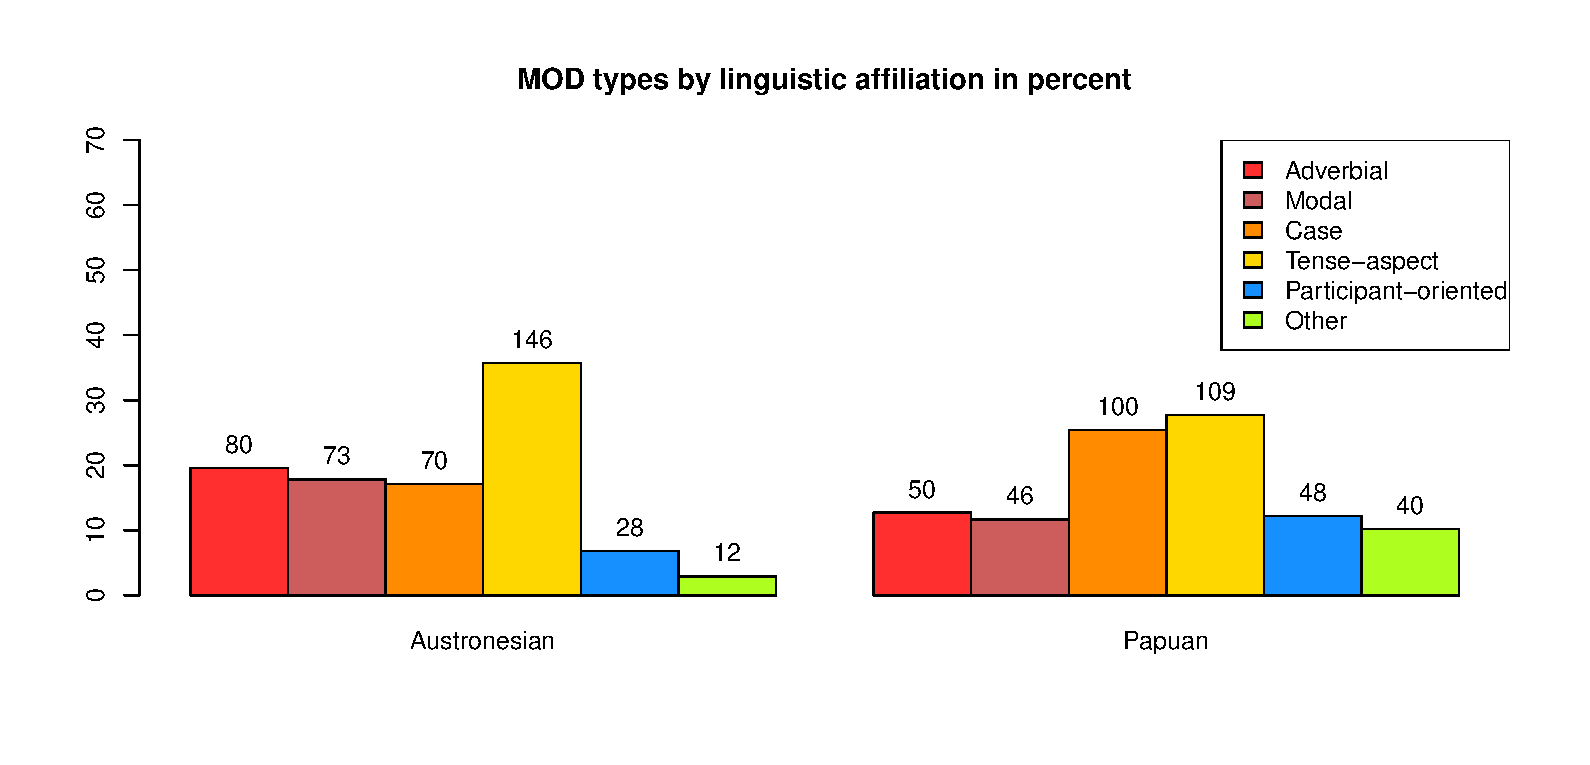
\includegraphics[width=\columnwidth]{figures/MOD_Family.eps}
\caption[MOD types by linguistic affiliation]{MOD types by linguistic affiliation. Numbers on top of the bars refer to the number of observations in the sample.}\label{fig:mod-family}
\end{figure}
\begin{figure}
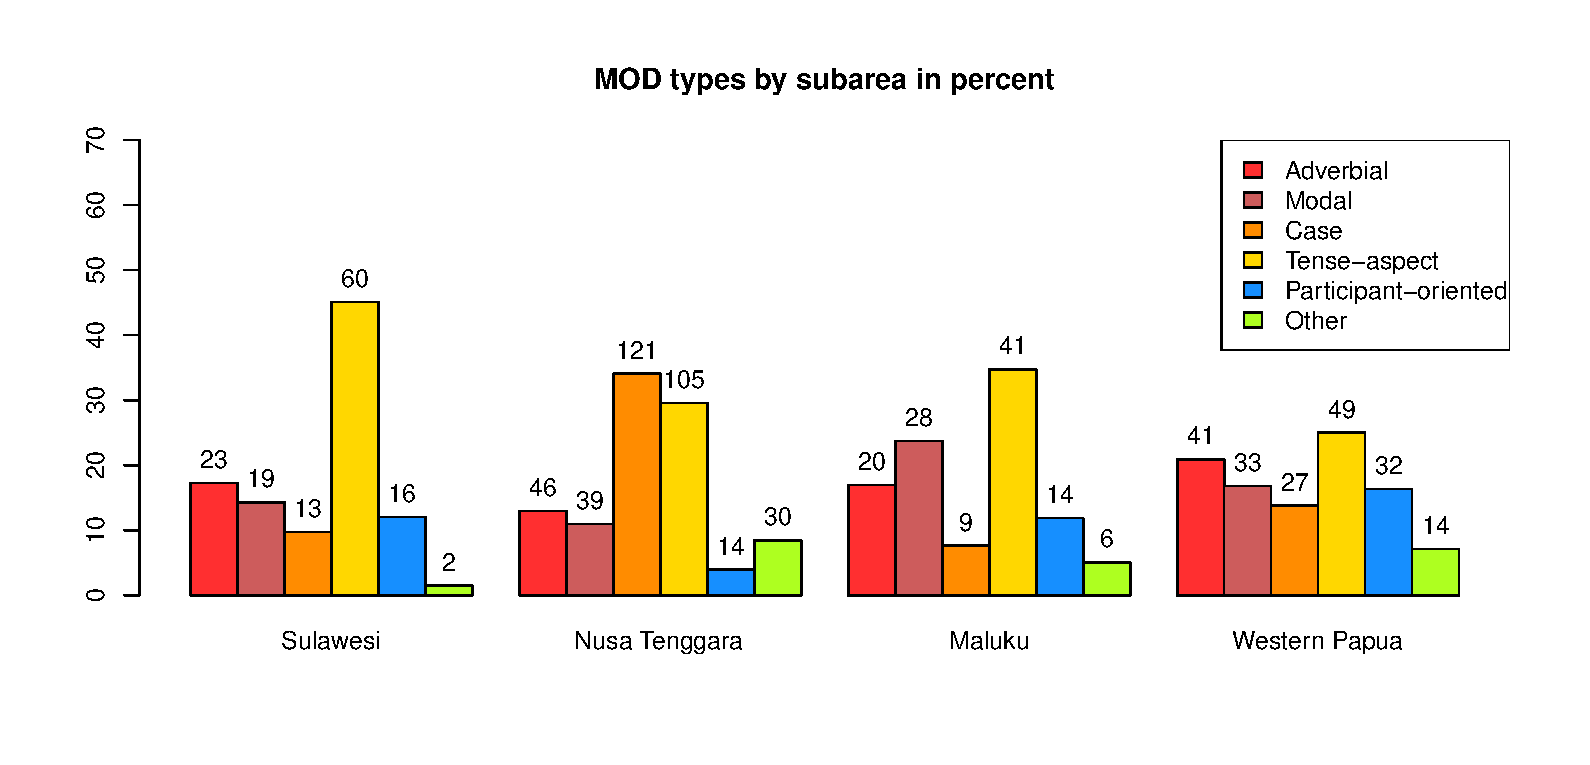
\includegraphics[width=\columnwidth]{figures/MOD_Group.eps}
\caption[MOD types by subarea]{MOD types by subarea. Numbers on top of the bars refer to the number of observations in the sample.}\label{fig:mod-group}
\end{figure}


%\tabref{table:MOD_language} below is a computation of MOD construction numbers by language. As might be expected, a more fine-grained resolution of MOD distribution across the sample reveals further patterns. In the Sulawesi languages we again find the by now familiar division into northern Sulawesi languages (Pendau, Tajio), envisaging very little use of MOD MVCs, and into the south-eastern languages for which MOD use is clearly a pervasive phenomenon. Some other languages also deviate from the general picture by only using one of the functional groups, and in very small numbers. For Alorese (\textsc{nus} subarea) and Abun (\textsc{pap}) only adverbial constructions could be found. Dusner only contributes observations of case-marking constructions to the sample. And finally, Sougb only has modal MOD constructions, or so the numbers suggest.

%\begin{table}
%\begin{footnotesize}
%\begin{tabular}{lrrrrrr}
%  \lsptoprule
%  & \multicolumn{4}{c|}{event-oriented} & & \\
% & {adverbial} & {modal} & {case} & {tense-aspect|} & {participant-oriented} & {other}\\ 
%  \midrule
%  Muna &   6 &   3 &   2 &  12 &   8 &   1 \\ 
%  Pendau &   0 &   1 &   0 &   3 &   1 &   0 \\ 
%  Tajio &   5 &   0 &   0 &   1 &   0 &   0 \\ 
%  Tolaki &   4 &   1 &   0 &  33 &   2 &   0 \\ 
%  TukangBesi &   8 &  14 &  11 &  11 &   5 &   1 %\\ \midrule
%  Abui &   3 &  14 &  30 &  15 &   3 &   8 \\ 
%  Alorese &   4 &   0 &   0 &   0 &   0 &   0 \\ %
%  Bunaq &  15 &   1 &   0 &  28 &   3 &   8 \\ 
%  Kaera &   0 &   0 &   2 &   0 &   0 &   2 \\ 
%  Kambera &   1 &   2 &  18 &   3 &   0 &   0 \\ %
%  Klon &   6 &   8 &  16 &   9 &   0 &   1 \\ 
%  Makalero &   5 &   5 &  28 &   4 &   1 &   5 %\\ 
%  Teiwa &   5 &   0 &   3 &   9 &   0 &   0 \\ 
%  Tetun &   0 &   0 &  13 &  10 &   3 &   0 \\ 
%  Waimaqa &   5 &   9 &   8 &  24 &   0 &   6 \\ %
%  WesternPantar &   2 &   0 &   3 &   3 &   4 & %  0 \\ \midrule
%  Buru &  12 &  11 &   0 &   9 &   1 &   0 \\ 
%  Selaru &   2 &   7 &   5 &   0 &   2 &   1 \\ 
%  Taba &   2 &   4 &   2 &  11 &   1 &   2 \\ 
%  Tidore &   4 &   4 &   2 &   8 &   2 &   3 \\ 
%  Tobelo &   0 &   2 &   0 &  13 &   8 &   0 \\ %\midrule
%  Abun &   1 &   0 &   0 &   0 &   0 &   0 \\ 
%  Biak &   5 &   7 &   0 &   2 &   2 &   0 \\ 
%  Dusner &   0 &   0 &   9 &   0 &   0 &   0 \\ 
%  Hatam &   0 &   0 &   0 &   1 &   5 &   0 \\ 
%  Inanwatan &   0 &   0 &   0 &   1 &   0 &   3 %\\ 
%  Maybrat &   0 &   3 &  15 &   3 &   8 &   1 \\ %
%  Mor &   1 &   1 &   0 &   3 &   2 &   0 \\ 
%  Moskona &   8 &   1 &   0 &  13 &   7 &   9 \\ %
%  Mpur &   1 &   5 &   1 &   2 &   7 &   0 \\ 
%  Sougb &   0 &   3 &   0 &   0 &   0 &   0 \\ 
%  Wooi &  25 &  13 &   2 &  24 &   1 &   1 \\ 
%   \midrule
%   \end{tabular}
%   \end{footnotesize}
%   \caption{Distribution of attested %MOD constructions across languages}
%\label{table:MOD_language}
%\end{table}

Turning to the morphosyntactic properties of MOD constructions, we find a much more diverse picture than with the component-relating constructions in the previous section. This is hardly surprising as the latter form a small set of uniform constructions that seem to exhibit little variation across EI. Modifying constructions, on the other hand, are a heterogeneous pool of constructions with similar functions that are strongly influenced by the respective source lexemes of the modifier verb, as well as the specific grammaticalisation cline. This leads to the picture illustrated by \tabref{table:mod_formal} below. The numbers show that the majority of MOD MVCs still conform to the default \textsc{MVC} that was discussed at the end of Chapter \ref{ch:gram}: a construction with arguments tied together in ``same subject" fashion, with inflection found on two verbs placed adjacent to each other. MOD constructions are also preferentially construed with the same subject pattern (the second most frequent argument configuration being event-to-argument reanalysis ``E"), a double-head marking is prevalent, and the verbs mostly appear in contiguous sequence. What is noticable, though, is that MOD constructions do not exhibit the same amount of variation with respect to contiguity (the two most extreme values, ``3" and ``4" constituents intervening, are missing).

\begin{table}
\centering
\begin{tabular}{rrrrrrr}
  \lsptoprule
Referentiality & S & SO & D & A & E & X \\ 
  \midrule
  adverbial &  74 &   2 &   6 &   0 &  48 &   0 \\ 
  modal &  95 &   0 &   0 &   1 &  16 &   7 \\ 
  case & 126 &   0 &  21 &   3 &  17 &   3 \\ 
  tense-aspect & 179 &   2 &   9 &   0 &  61 &   4 \\ 
  participant-oriented &  58 &   0 &  11 &   1 &   6 &   0 \\ 
  other &  27 &   0 &   4 &   0 &  20 &   1 \\ 
   \midrule
 \\
  \midrule
Headedness & B & 1 & 2 & S & N \\ 
  \midrule
  adverbial &  35 &  18 &   0 &  13 &   6 \\ 
  modal &  57 &   2 &   8 &   3 &   1 \\ 
  case &  25 &  21 &   1 &  19 &   1 \\ 
  tense-aspect &  71 &  48 &   4 &   8 &  13 \\ 
  participant-oriented &  52 &   1 &   1 &   4 &   3 \\ 
  other &  11 &   6 &   3 &   1 &   1 \\ 
   \midrule
 \\
  \midrule
Contiguity & W & C & 1 & 2 \\ 
  \midrule
  adverbial &   1 & 118 &  11 &   0 \\ 
  modal &   0 &  99 &  18 &   2 \\ 
  case &   0 & 127 &  43 &   0 \\ 
  tense-aspect &   4 & 220 &  27 &   4 \\ 
  participant-oriented &   0 &  58 &  16 &   2 \\ 
  other &   3 &  42 &   7 &   0 \\ 
   \lspbottomrule
\end{tabular}
\caption[Morphosyntactic properties of MOD constructions]{Morphosyntactic properties of MOD constructions in EI. Table components from top to bottom refer to referentiality (see §\ref{sec:argumentstructure}), headedness (see §\ref{sec:headedness}), and contiguity (see §\ref{sec:contiguity}), respectively. Referentiality values: S = Co-functional (``same subject"), SO = Transitive co-functional (``same subject and object"), D = Switch-function (``Different subject"), A = Participant accumulation, E = Event-to-argument (``Ambient"), X = no interaction, no arguments shared. Headedness values: B = Both verbs marked, 1 = First verb marked, 2 = Second/final verb marked, S = Shared affix set, N = None of the verbs marked. Contiguity values: W = Within word, C = Contiguous verbs 1 = One non-verbal constituent intervening, 2 = Two non-verbal constituents intervening, 3 = Three non-verbal constituents intervening, 4 = Four non-verbal constituents intervening.}
\label{table:mod_formal}
\end{table}

The following sections turn to the different functional groups introduced above, and provide examples from different constructions and subareas.

\subsection{Adverbial}\label{sec:adverbial}

Adverbial MOD constructions cover two groups of modifier verbs that fulfill `adverbial functions'. Adverbial constructions proper contribute adverb-semantics that in non-serialising languages such as English are expressed by adjectives or adverbs. In this group of MOD constructions, the modifying verb is recruited from a class of stative verbs. The second group, manner MODs, are made of what seem to be full-fledged verbs that are used in the modifier slot of the construction. As a heuristic, I assumed that such instances of MOD constructions could be translated with the help of the phrase ``do X in Y manner", where X is the matrix verb, and Y refers to the semantics of the modifying verb. \tabref{table:adverbial} presents the basic numbers. 

\begin{table}
\begin{tabular}{ll}
\lsptoprule
Feature&Value\tabularnewline
\midrule
Template&V1 \textsc{matrix verb} * V2 \textsc{modifier verb}\tabularnewline
No. of attested instances& 130/2146 \tabularnewline
No. of attested languages& 23/32 \tabularnewline
Distribution across areas& \textsc{sul} (4/5), \textsc{nus} (9/11), \textsc{mal} (4/5) \textsc{pap} (6/11) \tabularnewline
Distribution across families& \textsc{pap} (10), \textsc{aus} (13) \tabularnewline
\lspbottomrule
\end{tabular}
\caption[Template and basic distribution of adverbial MOD MVCs]{Template and basic distribution of adverbial MOD MVCs in the EI sample. The asterisk indicates that matrix verb and modifier verb may occur in both positions.}
\label{table:adverbial}
\end{table}

The percentages from \figref{fig:mod-group} above seem to indicate that adverbial modification is most widespread in the Western Papua languages. However, most instances come from just one language, the corpus language Wooi, and in fact only 6 of 11 \textsc{pap} languages display multi-verbal adverbial constructions. Wooi has two adverbial MVC constructions. First, there is a small class of stative verbs that are able to take inflection, and appear close to the matrix verb they modify. This pattern is illustrated in example (\ref{wooi_37}) with the modifier of speed, \textit{mararu}. The example consists of two MVCs, a motion complex formed by \textit{vavu} and \textit{taveri}, and a modifying construction where \textit{mararu} is added. Note that both the component-relating process as well as the modification by \textit{mararu} do not add further spatiotemporal stages to the event scheme. The third verb, \textit{taveri}, remains uninflected due to its deranked status within the motion complex, but would in other contexts inflect as well. As \textit{mararu} seems to modify the whole motion complex, I assume that the modifying construction forms only after the motion verbs merge their components. However, the exact scope of the modifier verb remains ambiguous in many examples. (Alternatively one might assume here that \textit{mararu} targets the matrix verb \textit{vavu}, and the whole modified motion construal is then specified by \textit{taveri}).

\ea \label{wooi_37}
\langinfo{Wooi}{Austronesian, SHWNG}{HIVIAY\_exp}\\
\glll tamararu tambavu taveri \\
ta-mararu ta-vavu taveri \\
1\textsc{pl}.\textsc{in}-fast 1\textsc{pl}.\textsc{in}-return.home return \\
\glft `(And) we (can) go home fast.'\\ 
\z

A second adverbial MVC pattern involves postverbs that do not normally appear without a matrix verb. These are always construed with a shared set of verbal affixes (which is not always visible if there is no resumptive object suffix attached to the postverb, such as \textit{-a} below). Example (\ref{wooi_30}) is a typical case.

\ea \label{wooi_30}
\langinfo{Wooi}{Austronesian, SHWNG}{MANTERA\_magic\_charms}\\
\glll tatong harata mara \\
ta-ong hara=a mara \\
1\textsc{pl}.\textsc{in}-use wrong=\textsc{obj}.\textsc{nsg} \textsc{top} \\
\glft `If we use it wrongly...'\\ 
\z

A number of EI languages derives such modifiers by way of reduplication, and they are mostly considered adverbs, not verbs proper. This is why examples like the following one from Kaera have been excluded from the sample. Note, however, that in some languages ``adverbial" modifiers are treated as verbs (by the respective authors) despite their reduplicated form, as in example (\ref{Bunaq17}) from Bunaq. The distribution of adverbial MVCs would thus be more widespread in EI if all instances of reduplicated modifiers were counted as verbs.\footnote{Excluding all instances of reduplication in verbs would not be helpful either, as this would also pertain to dynamic verbs, where reduplication in EI frequently produces Aktionsart differences, such as iterative or intensive readings.}

\ea 
\langinfo{Kaera}{Papuan, TAP}{\citealt[138]{klamer2014kaera}}\\
\gll ging kali~kali ekeng \\
3\textsc{pl} \textsc{rdp}~slow climb.up \\
\glft `They climb up slowly.'\\ 
\z

\ea \label{Bunaq17}
\langinfo{Bunaq}{Papuan, TAP}{\citealt[451]{schapper2009bunaq}}\\
\gll leleq enoq~enoq \\
flow slow~\textsc{rdp} \\
\glft `(The water) runs really slowly.'\\ 
\z

Manner constructions are formed by combining LLEs from two active verbs, most of them process verbs. The verbs that are in modifying function can also appear in simplex predicates elsewhere. Two major semantic fields may be distinguished. First, motion LLEs are modified by verbs denoting manner of motion, or otherwise compatible concepts that can be carried out during the motion process. Example (\ref{Bunaq_87}) from Bunaq illustrates such a case where the second verb provides information on the intention of the motion process (``in flight"). 

\ea \label{Bunaq_87}
\langinfo{Bunaq}{Papuan, TAP}{\citealt[472]{schapper2009bunaq}}\\
\gll Tebe tama sai, borus ciwal liol \\
return enter exit move.through flee continue \\
\glft `In turn (she) went in (then) out, continuing going through in flight.’\\ 
\z

Second, verbs of searching are quite often found in modifying function. The Biak case in (\ref{Biak_18}) shows such a construal, again together with a motion LLE, forming a motion PLE with manner specification. Verbs of searching are, however, also found accompanying non-motion verbs (for instance, \textsc{call} someone in a searching manner).

\ea \label{Biak_18}
\langinfo{Biak}{Austronesian, SHWNG}{\citealt[189]{vanheuvel2006}}\\
\glll Rofan anine ifrar syéwaro romámkun anine \\
rofan an-i-ne i-frar s$<$y$>$éwar=o romá-mkun an-i-ne \\
dog \textsc{giv}-3\textsc{sg}.\textsc{spec}-this 3\textsc{sg}-run $<$3\textsc{sg}$>$seek=O child-little \textsc{giv}-3\textsc{sg}.\textsc{spec}-this \\
\glft `This dog ran seeking for this child.'\\ 
\z

\subsection{Modal}\label{sec:modal}

Modal MOD constructions convey a range of functions that are expressed in non-serialising languages by modal verbs, interrogative pronouns, permissives, and evidential and hypothetical elements, among others. The functional common ground of all these is that the default factual mode of the utterance is modified, either in terms of agent-related properties (desiderative, abilitative, deontic), with respect to event status (evidential, hypothetical, conative), or discourse-related (interrogative, hortative). The two latter functions are only rarely attested in the EI sample for very few languages; the bulk of modal MOD constructions refer to agent-related modification, that is desiderative, abilitative, and, to a lesser degree, deontic semantics. \tabref{table:modal} summarizes the main facts about the distribution of MOD constructions across EI, showing that the majority of EI languages utilise MOD MVCs at least for some of the functions.

\begin{table}
\begin{tabular}{ll}
\lsptoprule
Feature&Value\tabularnewline
\midrule
Template&V1 \textsc{matrix verb} * V2 \textsc{modifier verb}\tabularnewline
No. of attested instances& 119/2146 \tabularnewline
No. of attested languages& 22/32 \tabularnewline
Distribution across areas& \textsc{sul} (4/5), \textsc{nus} (6/11), \textsc{mal} (5/5) \textsc{pap} (7/11) \tabularnewline
Distribution across families& \textsc{pap} (11), \textsc{aus} (11) \tabularnewline
\lspbottomrule
\end{tabular}
\caption[Template and basic distribution of modal MOD MVCs]{Template and basic distribution of modal MOD MVCs in the EI sample. The asterisk indicates that matrix verb and modifier verb may occur in both positions.}
\label{table:modal}
\end{table}

Two main groups may be distinguished: (i) constructions with pseudo-modals that resemble modal verb constructions (but do not show the usual distinctions in finiteness), and (ii) adverb- or pronoun-like elements that morphosyntactically behave like verbs (or are treated as such by the respective data sources). The following examples illustrate typical constructions from the first group. The pair of examples in (\ref{Taba_29}) and (\ref{Taba_30}) from Taba exemplify what I take to be a core property of MOD constructions, at least in prototypical cases: that the modifying constituent has gained the status of an independent constituent under the grammaticalisation process, and may occur in different positions within the clause (if the respective language does not require absolutely rigid constituent order in the clause). In the Taba example, neither the principle of iconic ordering nor any other rigid constructional template constrains the use of \textit{ahan}. Although this freedom of ordering does not exist in many other instances of MOD constructions, it could be predicted that MOD constructions in different languages grammaticalising similar lexemes display differential ordering of matrix verb and modifier verb (depending on the source lexeme, and its original position). This variation sets MOD constructions apart from component-relating and stage-relating constructions, which are always guided by general ordering principles.

\ea \label{Taba_29}
\langinfo{Taba}{Austronesian, SHWNG}{\citealt[316]{bowden2001taba}}\\
\glll npe nahan \\
n=pe n=ahan \\
3\textsc{sg}=do 3\textsc{sg}=be.able \\
\glft `He can do it.'\\ 
\z

\ea \label{Taba_30}
\langinfo{Taba}{Austronesian, SHWNG}{\citealt[316]{bowden2001taba}}\\
\glll wwe nahan ncagal \\
wwe n=ahan n=sagal \\
leg 3\textsc{sg}=be.able 3\textsc{sg}=step \\
\glft `My leg would be able to walk.'\\ 
\z

The most frequent cases of pseudo-modals are desiderative constructions that express desire, want, or intention of the actor to perfom the action contributed by the matrix verb. Here are two examples from different subareas. The first example in (\ref{Bunaq_2}) shows the only case in the sample where the desiderative verb comes second and not first (despite the fact that Bunaq is an AVO language). Recall from §\ref{sec:criteria_mvcs} that modifying constructions do not show constant behaviour in terms of operator placement. While TAM and person indexing operator values are typically shared across all verbal constituents in MOD constructions, this is not true for negation, where at least in some MOD constructions, negation of just one constituent seems possible. The Bunaq example in (\ref{Bunaq_2}) reflects this behaviour as the prospective marker \textit{gie} here only targets the motion constituent. This is in contrast to component-relating and stage-relating constructions in Bunaq where operators such as \textit{gie} need to have scope over the entire construction (cf. \citealt[443f.]{schapper2009bunaq}).

\ea \label{Bunaq_2}
\langinfo{Bunaq}{Austronesian, TAP}{\citealt[444]{schapper2009bunaq}}\\
\gll baqi o mal gie heten \\
\textsc{nprx}.\textsc{an} \textsc{foc}.\textsc{add} go \textsc{prosp} want \\
\glft `She also wants to walk.’\\ 
\z

Example (\ref{Wooi111}) from Wooi illustrates the order desiderative verb -- matrix verb. At least in Wooi, this order reflects  original source properties of the modifier verb. The origin of \textit{o} `want' is still transparent in Wooi: it is derived from \textit{oyo} `say' which is also frequently attested in a short form \textit{o} (\textit{o} `want', however, is always short, and never appears as \textit{oyo}). Thus desiderative constructions with \textit{o} originated from speech complement constructions where the sentential complement followed the \textsc{say} verb (and eventually got reanalysed as matrix verb constituent of a desiderative construction).

\ea \label{Wooi111}
\langinfo{Wooi}{Austronesian, SHWNG}{HIVIAY\_exp}\\
\glll co vio to Nunoing vane \\
ti-o $<$i$>$vo to Miosnum vane \\
3\textsc{sg}-want $<$3\textsc{sg}$>$row \textsc{dir} Miosnum \textsc{det}.\textsc{nprx} \\
\glft `(For example, if) he wants to go to Miosnum...'\\ 
\z

Speech act complementation can have a shift in subject arguments (for instance, in \textit{I say you do} type constructions). Given that speech act complementation is the source of at least some of the desiderative MVCs coded here as MODs, this raises the question whether desideratives of this sort can have the same shift in arguments. In English, \textit{want} constructions are overtly biclausal, and involve raising of the dependent clause subject to the object of the matrix clause in case the ``wisher" is not co-referential with the referent that is supposed to perform the action. Think of something like \textit{I want Jones to butter his toast at midnight} where, in structural terms, Jones belongs to the subordinate clause but is raised to object status. Such constructions are also possible in some EI languages with the only difference that there is no cue as to a biclausal construal. Consider an example from Selaru.

\ea \label{Selaru_4}
\langinfo{Selaru}{Austronesian, CMP}{\citealt[112]{coward2005}}\\
\gll Majelis-ke r-buma ta-wahuk nur-Vre rahean.rahean \\
elders-\textsc{art} 3\textsc{pl}-want 1\textsc{pl}.\textsc{in}-gather coconut-\textsc{pl} ten.by.ten \\
\glft `The church elders want us to gather coconuts in tens.‘\\ 
\z

In Selaru both same-subject desiderative constructions, as well as ones without argument sharing, as in (\ref{Selaru_4}), are equally licit. Argument interaction in such examples has been coded ``X" as the exact argument relation between the constituents is not made transparent by morphosyntactic marking (note that such examples explain the conspicuous number of 7 ``X" cases for modal MOD constructions in \tabref{table:mod_formal} above). This is, however, not the case in all languages. Wooi is different in this regard. We might expect to find a conceptual overlap between speech act complements (`I say he takes'), and desiderative readings (`I want him to take'), but this is not supported by the Wooi data corpus. Whenever there is a shift in subject indexing between \textsc{say}/\textsc{want} and matrix verb, the translation given indicates that the construction is still understood in its literal sense as a speech complement.\footnote{Note that the interrelatedness between cognitive verbs like \textsc{wish} and speech verbs like \textsc{say} reflects the deeper cultural doctrine of the ``opacity of other minds" that is well-developed in many languages from New Guinea and parts of Oceania. Opacity of the other mind describes what can be perceived as a cultural reluctance of stating directly what other people think or believe, as this is deemed impossible to know from an outside perspective. Instead of saying, for instance, \textit{Jones wants to eat toast at midnight}, one would rather resort to a behaviorist interpretation \citep{robbins2008not} like \textit{Jones says he eats toast at midnight}, thus circumventing a direct statement about Jones' inner feelings. See \citet{robbins2008introduction, robbins2008not, rumsey2013intersubjectivity} on the opacity of other minds.}

Turning to the second group of modal MOD constructions, we find adverb- or pronoun-like elements that take inflection and behave like a fully fledged verb. These MODs are rare in the sample and basically confined to south-eastern Sulawesi and some odd examples from Papuan languages of the TAP area (Abui, Makalero). The following examples from Tukang Besi show an interrogative pronoun with verb-like behaviour in (\ref{Tukang_17}), and an inflected evidential element in (\ref{Tukang_18}). Comparable constructions are otherwise hardly found in the sample.

\ea \label{Tukang_17}
\langinfo{Tukang Besi}{Austronesian, WMP}{\citealt[191]{donohue1999}}\\
\gll o-ha'a tabeda to-wila loeloe? \\
3\textsc{rls}-why necessary 1\textsc{pl}.\textsc{rls}-go slowly \\
\glft `Why will we have to go slowly?'\\ 
\z

\ea \label{Tukang_18}
\langinfo{Tukang Besi}{Austronesian, WMP}{\citealt[189]{donohue1999}}\\
\gll o-tantu no-rato sabentara \\
3\textsc{rls}-certain 3\textsc{rls}-arrive in.a.moment \\
\glft `They'll be here in a moment for certain.' (i.e., `It is certain they will arrive in a moment.')\\ 
\z

\subsection{Case-marking} \label{sec:case-marking}

Case-marking is here understood in a non-strict sense: case-marking MOD constructions comprise all those cases in which a (transitive) modifier verb introduces a further argument to the argument frame of the construction. This argument typically belongs to a set of oblique (adjunct) arguments, but some constructions seem to introduce core arguments as well. Attested arguments are direct object (patient, theme), experiencer, recipient, benefactive, comitative, instrumental, locative, source, and goal. Such MVCs have been identified in many serialising languages and can be considered one major group of prototypical SVCs according to many analyses (for instance \citealt{givon1991serial, Aikhenvald2006, haspelmath2016serial}; see also \citealt{lord1993historical} on the diachronic development of case-marking constructions in African languages). \tabref{table:case} illustrates the basic facts on the distribution of case-marking MVCs across the EI area.

\begin{table}
\begin{tabular}{ll}
\lsptoprule
Feature&Value\tabularnewline
\midrule
Template&V1 \textsc{matrix verb} * V2 \textsc{modifier verb}\tabularnewline
No. of attested instances& 170/2146 \tabularnewline
No. of attested languages& 18/32 \tabularnewline
Distribution across areas& \textsc{sul} (2/5), \textsc{nus} (9/11), \textsc{mal} (3/5), \textsc{pap} (4/11) \tabularnewline
Distribution across families& \textsc{pap} (9), \textsc{aus} (9) \tabularnewline
\lspbottomrule
\end{tabular}
\caption[Template and basic distribution of case-marking MOD MVCs]{Template and basic distribution of case-marking MOD MVCs in the EI sample. The asterisk indicates that matrix verb and modifier verb may occur in both positions.}
\label{table:case}
\end{table}

As I have already noted above, case-marking MVCs can be considered a special feature of the Nusa Tenggara subarea, as 121 from 170 instances are from \textsc{nus} languages. Nine of 11 Nusa Tenggara languages have such constructions, with Abui and Makalero being particularily productive in this regard.

Introduction of direct object arguments is only found in Makalero. The \textsc{take} verb \textit{mei} has developed into a light verb introducing arguments in case the object slot of the main verb is already taken, for instance by a member of the large complement class \citep[203f.]{huber2011}. Verbal argument frames in Makalero may not exceed two arguments. Therefore, when the object slot is in use, the addition of another argument slot is brought about by employing \textit{mei}. Examples (\ref{Makalero_56}), (\ref{Makalero_61}), and (\ref{Makalero_18}) illustrate three instances where the light verb \textit{mei} is used. Each one adds a different kind of argument to the argument frame of the construction, making \textit{mei} a valency increaser with a broad range of functional contexts. In example (\ref{Makalero_56}), \textit{mei} introduces the object-theme \textit{Timor} because the ``complement-verb complex" (see \citealt[131f.]{huber2011}) consisting of matrix verb \textit{kini/ini} `do' and its complement \textit{lafu'} already constitute a saturated transitive argument frame. Note that Makalero has two kinds of linkers, \textit{=ini} and \textit{=isi}, both of which Huber analyses as clause linkers \citep[457f.]{huber2011}. Given, however, that at least \textit{=ini/ni} often appears in positions that obviously connect verbs of tightly bound constructions, I am assuming here that \textit{=ini/ni} rather provides a means to overtly extablish an integral construction rather than marking off two different clauses. Its use appears to be optional rather than required by the light verb, as examples (\ref{Makalero_61}) and (\ref{Makalero_18}) are grammatical without a linker.

\ea \label{Makalero_56}
\langinfo{Makalero}{Papuan, TAP}{\citealt[169]{huber2011}}\\
\gll negara taure’=ini tone’ ma’u=ni Timor ere mei=ni lafu’-ini \\
nation which=\textsc{ctr} perhaps come=\textsc{lnk} T. 1\textsc{dem} take=\textsc{lnk} live-do:\textsc{bd} \\
\glft `...whichever nation comes and rescues Timor...’\\ 
\z

The next example in (\ref{Makalero_61}) shows the introduction of another theme-object. According to Huber's analysis, the object argument added by \textit{mei} is read as an instrument \citep[204]{huber2011}. This is indeed the case, but only at the level of the construction. It is the context, rather than \textit{mei} itself, that invokes the instrument reading of the referent.

\ea \label{Makalero_61}
\langinfo{Makalero}{Papuan, TAP}{\citealt[204]{huber2011}}\\
\gll Nana-uai aire’ sa’a-mei tina-ini? \\
elder.sibling-\textsc{hon} now what:\textsc{bd}-take cook-do:\textsc{bd} \\
\glft ‘With what are you cooking?’\\ 
\z

Another use of \textit{mei} is in complex argument frames pertaining to construals of perception. In example (\ref{Makalero_18}) \textit{fi lolo-ini ere}, `our language', is the stimulus of the perception event. It is first introduced by transitive \textit{mei}, and then, as I understand it, reintroduced as subject argument of an intransitive \textit{puna} `look'. So, literally, I would expect something along the lines of `our language, we take (it), it looks very bad'.

\ea \label{Makalero_18}
\langinfo{Makalero}{Papuan, TAP}{\citealt[189]{huber2011}}\\
\gll po fi lolo-ini ere fi=haka e’=ini mei puna hanu pa’u$~$pa’uk \\
\textsc{adv} 1\textsc{pl}.\textsc{in} say-\textsc{nm} 1\textsc{dem} 1\textsc{pl}.\textsc{in}=\textsc{ctrpres} \textsc{dem}=\textsc{lnk} take look very \textsc{rdp}$~$bad \\
\glft ‘But our language, we see it as very bad...’\\ 
\z

Up to this point, no examples have been contributed by the other EI languages. They only enter the picture when we turn to the introduction of adjunct arguments. Here we may distinguish two groups: (i) circumstantial arguments involving benefactives, comitatives, and instruments; (ii) and local arguments, namely source, locative, and goal arguments. Benefactive MVCs occur in four languages, Tukang Besi from the Sulawesi group, Makalero and Abui from Nusa Tenggara, and the language isolate Maybrat from Western Papua. I have already illustrated benefactive MVCs from these languages in §\ref{sec:modification} on the semantics of modification.

Comitative and instrument constructions are more common throughout EI, but it is still only a minority of languages that have attested examples. Both groups of constructions may use a modifier verb that is glossed as `with' (among other verbs that are specific to either constructional group, such as \textsc{accompany} verbs in comitative constructions). Maybrat even employs two different \textsc{with} verbs, one for each construction. Comitatives are attested for Tukang Besi, Abui, Western Pantar, Tetun Fehan, Waima'a, Teiwa, Selaru, and Maybrat. The following pair of examples from Tetun again shows that at least some of the modifying MVCs allow the modifier consituent to be placed either before or after the matrix verb. At first glance the pattern seems identical, as \textit{hó} `accompany' follows the directed motion verb \textit{bá} in each case. In example (\ref{Tetun_54}), however, the modifier verb is ordered after the matrix verb, while example (\ref{Tetun_57}) shows what I take to be a case of stacked MVCs: the modifying construction is nested into the action slot of a matrix motion-to-action MVC. Thus, the order \textit{bá} \textit{hó} looks just the same in both examples, but the directed motion verb in example (\ref{Tetun_57}) is in fact not part of the modifying construction. That is, in example (\ref{Tetun_57}) the modifier verb is preposed to its matrix verb \textit{k-adiuk}. This analysis is supported by van Klinken's own analysis (cf. \citealt[272]{vanklinken1999grammar}): the comitative relation only holds true at the time of the playing, but not at the precursor motion phase.

\ea \label{Tetun_54}
\langinfo{Tetun Fehan}{Austronesian, CMP}{\citealt[272]{vanklinken1999grammar}}\\
\gll ha'u bá k-ó lós Am Bo'uk dei \\
1\textsc{sg} go 1\textsc{sg}-accompany just father Bo'uk only \\
\glft `I will go with only Am Bo'uk. (i.e. no-one else will go)'\\ 
\z

\ea \label{Tetun_57}
\langinfo{Tetun Fehan}{Austronesian, CMP}{\citealt[272]{vanklinken1999grammar}}\\
\gll ha k-bá k-ó feto sia k-adiuk \\
1\textsc{sg} 1\textsc{sg}-go 1\textsc{sg}-accompany woman \textsc{pl} 1\textsc{sg}-play \\
\glft `[Every evening,] I go and play with (i.e. court) the girls.'\\ 
\z

Note that \textit{hó} still appears to maintain a more concrete lexical meaning than, say, a verb that is only glossed as `with'. The next example is from Selaru, and shows such a case with a stripped-down comitative verb. Note again that comitative verbs may come either before or after the matrix verb, at least from a crosslinguistic perspective. This is in sharp contrast to what we find with both component-relating and stage-relating constructions.

\ea 
\langinfo{Selaru}{Austronesian, CMP}{\citealt[120]{coward2005}}\\
\gll Y-aso sir ma r-al-a kotw ti enen desike y-or amam desike ra ma ktei \\
3\textsc{sg}-request them \textsc{conj} 3\textsc{pl}-give-Ø food \textsc{conj} woman that(\textsc{art}) 3\textsc{sg}-with man that(\textsc{art}) they.eat until done \\
\glft `He requested they give the food so that woman and that man [can] eat until done...'\\ 
\z

Instrumental MVCs are attested for Kambera, Klon, Tetun Fehan, Taba, Tidore, and Maybrat. In Kambera, instrumental MVCs are construed with a \textsc{use} verb, \textit{wàngu}. Here are three examples. In (\ref{Kambera_22a}), \textit{wàngu} is placed after the matrix verb, and this is the default position. In case the \textit{wàngu} VP is topicalised, it can precede the matrix verb, however, by changing its syntactic status through the use of a linker \textit{ba}, as example (\ref{Kambera_22b}) shows. Another possible manipulation of (\ref{Kambera_22a}) is focusing of the instrument argument licensed by \textit{wàngu}. Preposing \textit{huru}, the spoon, in example (\ref{Kambera_22c}) leaves the orginal order with a postposed \textit{wàngu} intact. One could argue that the Kambera case with \textit{wàngu} is just the same as the Makalero light verb \textit{mei} in that both modifier verbs license a direct object argument. The reason for placing \textit{mei} in the direct object group above, and \textit{wàngu} in the instrumental argument group, is that the former must have (at least originally) taken a theme object, while a \textsc{use} verb could arguably pass instrument semantics on to its object argument.\footnote{Kambera \textit{wàngu} is in fact one of those generic verbs that are hard to pin down semantically. It may in simplex predicate contexts have the meaning `use', `do', `say' (and, derived from say, `want'; \citealt[284ff.]{klamer1998grammar}). Therefore, placing the \textit{wàngu} construction in the group of instrumental MVCs heavily relies on the gloss `use'.}

\ea 
\langinfo{Kambera}{Austronesian, CMP}{\citealt[287]{klamer1998grammar}}\\
\ea \label{Kambera_22a}
\gll ku-taku uhu wàngu huru \\
1\textsc{sg}.\textsc{nom}-scoop rice use spoon \\
\glft `I scoop rice with a spoon.' \\ 
\ex \label{Kambera_22b}
\gll wàngu huru ba ku-taku uhu \\
use spoon \textsc{conj} 1\textsc{sg}.\textsc{nom}-scoop rice \\
\glft `With a spoon I scoop rice.' \\ 
\ex \label{Kambera_22c}
\gll huru ku-taku uhu wàngu \\ 
spoon 1\textsc{sg}.\textsc{nom}-scoop rice use \\
\glft `I scoop rice with a SPOON.'\\ 
\z
\z

The group of local case-marking constructions (source, locative, goal) is better attested than the other case-marking constructions. They are mainly formed by the use of a locative verb (mostly glossed as `be', `be.in', `be.at'). What is interesting is that the position of the locative verb often indicates its function by obeying the iconicity of order. That is, a preposed locative verb marks source arguments, and a postposed locative verb may mark a goal (see also \citealt{schapper2011iconicity} on source and goal encoding in Kamang and Bunaq). In Papuan head-final languages, however, the goal argument (with the locative verb) is usually placed before the matrix verb, indicating the somewhat grammaticalised nature of the modifier VP.

The first pair of examples in (\ref{Maybrat_60}) is from Maybrat, and illustrates a MVC introducing a source argument. Here, again, the order of both verbs seems interchangeable. Example (\ref{Abui_24}) is a source-marking construction from Abui. Locative verbs such as \textit{mi} are widespread across the TAP languages, and can express a range of different concepts, most of which are related to spatial semantics. When Abui \textit{mi} is construed with a motion verb, it marks the source or starting point of the motion process. Similar constructions can also be noticed in neighbouring languages, but sometimes a source NP is in fact lacking where it might be expected. Example (\ref{Klon_48}) illustrates such a case from Klon. It might be interpreted as covert source-marking: \textit{mi} adds a spatial starting point to the process of getting up, although no explicit mention is made of its exact location in the discourse space.

\ea \label{Maybrat_60}
\langinfo{Maybrat}{Papuan, isolate}{\citealt[206]{dol2007grammar}}\\
\ea
\gll t-ama t-pat Sorong \\
1\textsc{sg}-come 1\textsc{sg}-from S. \\
\glft `I come from Sorong.' \\ 
\ex
\gll ait y-pat rapuoh y-ama \\ 
3\textsc{m} 3\textsc{m}-from forest 3\textsc{m}-come \\
\glft `He comes from the forest.'\\ 
\z
\z

\ea \label{Abui_24}
\langinfo{Abui}{Papuan, TAP}{\citealt[356]{kratochvil2007grammar}}\\
\gll fala mi-a yaa! \\
house be.in-\textsc{dur} go \\
\glft `Go from the house!', lit. `Be in the house, go!’\\
\z

\ea \label{Klon_48}
\langinfo{Klon}{Papuan, TAP}{\citealt[137]{baird2008grammar}}\\
\gll nang bo adob lega mi ihih \\
\textsc{neg} \textsc{seq} true 3\textsc{sg}.\textsc{top} be.at get.up \\
\glft `So he indeed got up.'\\ 
\z

In Klon, modifier VPs with \textit{mi} can also occur postverbally, where they typically mark the endpoint or goal of a motion event. In example (\ref{Klon_99a}) below, we see that \textit{mi} may introduce local case NPs. Note that the NP \textit{alah} `house' is governed by \textit{mi}, and not by \textit{qad} `come'. The next example from Klon in (\ref{Klon_99b}) illustrates that the case interpretation of the NP licensed by \textit{mi} depends on the semantics of the matrix verb. The first instance is quite naturally interpreted as the endpoint of ego returning to the place called Hwak. The second \textit{mi}, however, combines with a stative verb and specifies the location of the sleeping.

\ea \label{Klon_99a}
\langinfo{Klon}{Papuan, TAP}{\citealt[137]{baird2008grammar}}\\
\gll kuur angkol a~awar qad alah mi ik \\
dog self \textsc{rdp}~return come house be.at \textsc{compl} \\
\glft `The dog itself came back and was at home.'\\ 
\z

\ea \label{Klon_99b}
\langinfo{Klon}{Papuan, TAP}{\citealt[148]{baird2008grammar}}\\
\gll na lam gen u-elel, eben buur u-elel, Hwak mi awar, Hwak weer mi taa' \\
1\textsc{sg}.\textsc{act} walk until \textsc{vi}-search village flat \textsc{vi}-search Hwak be.at return Hwak river be.at sleep \\
\glft `I walked until I found, found a flat village and returned to Hwak, slept at Hwak river.'\\ 
\z

\subsection{Tense-Aspect}

The largest group of MOD MVCs is formed by constructions that convey tense-aspect semantics (again understood here in a non-strict sense including Aktionsart concepts and all sorts of other temporal formatives), subsuming a wide range of different concepts. As in the modal group above, there are two sets of items that participate in such MOD constructions. First, there is a large group of aspectual verbs that have been grammaticalised to different extents. And second, there is a much smaller group of adverb-like elements that behave like verbs and denote temporal concepts. The latter group is again more or less confined to the languages of south-eastern Sulawesi (Tolaki, Muna, and Tukang Besi). \tabref{table:tense-aspect} below presents the basic numbers of tense-aspect MOD MVCs.

\begin{table}
\begin{tabular}{ll}
\lsptoprule
Feature&Value\tabularnewline
\midrule
Template&V1 \textsc{matrix verb} * V2 \textsc{modifier verb}\tabularnewline
No. of attested instances& 255/2146 \tabularnewline
No. of attested languages& 26/32 \tabularnewline
Distribution across areas& \textsc{sul} (5/5), \textsc{nus} (9/11), \textsc{mal} (4/5) \textsc{pap} (8/11) \tabularnewline
Distribution across families& \textsc{pap} (13), \textsc{aus} (13) \tabularnewline
\lspbottomrule
\end{tabular}
\caption[Template and basic distribution of tense-aspect MOD MVCs]{Template and basic distribution of tense-aspect MOD MVCs in the EI sample. The asterisk indicates that matrix verb and modifier verb may occur in both positions.}
\label{table:tense-aspect}
\end{table}

The group of aspectual verbs is dominated by \textsc{begin}, \textsc{finish}, and \textsc{complete} verbs. I coded constructions that focus on modifying the telicity of event construals (that is, denoting their beginning or ending) as aspectual proper, and distinguished another group of constructions (basically also involving verbs of finishing) that show signs of grammaticalisation towards completive semantics (that is, denoting actions affecting the totality of participants; see also \citealt{huber2014} on data from Bunaq, Kamang, and Makalero). Iconicity seems to be a factor in the formation of such MVCs, as \textsc{begin} verbs normally precede the matrix verb, and \textsc{finish} verbs follow it. The following examples give an illustration of how such aspectual MOD constructions look like in EI. Example (\ref{Tolaki_38}) is from Tolaki, and makes use of the inflection pattern typical for that language: only the first verb takes inflection, which is in this case the modifier verb (this order is, as I mentioned above, an exception among the EI  languages, as \textsc{finish} verbs typically come last). The next example in (\ref{Western_14}) is from Western Pantar, and illustrates two intertwined MVCs. The dying is construed as the direct result of the slicing by means of a stage-relating MVC. To this bi-stage event schema, an aspectual MOD MVC is added, reinforcing the endpoint of the dying. \textit{Gaata} here might either be interpreted as modifying \textit{hinna} alone, that is, the second event stage, or it might be read as modifying the whole event schema, that is, both stages. As the latter interpretation would clash with the conceptual event hierarchies, as proposed in chapter \ref{ch:sem}, I assume that in such cases, only the event stage adjacent to the modifier verb is modified (yielding something like slice -- [die finish]) (but see also §\ref{sec:clauselevelmodification}).

\ea \label{Tolaki_38}
\langinfo{Tolaki}{Austronesian, WMP}{\citealt[123]{mead2008verb}}\\
\gll Ari-'aku-to mong-gaa\\
finish-1\textsc{sg}.\textsc{abs}-prfv $<$M$>$:\textsc{antip}-eat \\
\glft `I've already eaten.'\\ 
\z

\ea \label{Western_14}
\langinfo{Western Pantar}{Papuan, TAP}{\citealt[82]{holton2014western}}\\
\gll a-ule pai hinna kanna gaata \\
4\textsc{sg}-neck slice die finish already \\
\glft `They sliced his neck and killed him.'\\ 
\z

Example (\ref{Buru_35}) from Buru illustrates the case of aspectual MVCs with a \textsc{begin} verb. In Buru and elsewhere, \textsc{begin} verbs precede their matrix verb, but the position of the pronominal subject is less rigid, and may shift to a position between the two verbs (see \citealt[215]{grimes1991buru}). The following example from Moskona exemplifies the use of a non-prototypical modifier verb. I have at several points made mention of motion verbs attaining aspectual semantics. In Moskona, it is obvious that \textit{eyja} still retains part of its motion semantics, but it may also be read as highlighting the beginning of an event. This relation between a stage-relating interpretation (go-build), and a modifying one (begin-build) sheds light on the diachronic pathways that exist between the different techniques of MVC formation. As constructions acquire new readings they may also acquire a different interpretation of their underlying event construal (for instance, by shifting from a bi-stage event schema to a mono-stage one).

\ea \label{Buru_35}
\langinfo{Buru}{Austronesian, CMP}{\citealt[215]{grimes1991buru}}\\
\gll ringe peltanek iko boli fena-fena \\
3\textsc{sg} begin go perimeter \textsc{rdp}-village \\
\glft `He began to go around to each of the villages.'\\ 
\z

\ea \label{Moskona_48}
\langinfo{Moskona}{Papuan, EBH}{\citealt[297]{gravelle2010grammar}}\\
\gll edá, eri i-eyja i-or mod jig merga or-i-em tas \\
then they.\textsc{pl} 3\textsc{pl}-go 3\textsc{pl}-build house \textsc{loc} wood \textsc{num}:7-?-\textsc{contr} again \\
\glft `Then, they began again to build a house in another tree.’ \\
or `they went again [and] built a house in another tree.’\\ 
\z

Completives differ from \textsc{finish} semantics in that the endpoint of the event is not reached by some actor willfully ending it, but because a totality of referents is affected (see e.g. \citealt{bybee1994evolution} for a diachronic assessment of completives). Not all EI authors distinguish between completives and \textsc{finish} semantics. The difference, however, stands out clearly when the glossing or translation of \textsc{finish} verbs involves some meaning of `all', as for instance in Waima'a \textit{maa}, or in the  \textit{kay} construction from Wooi. Waima'a \textit{maa} is most often translated as `finish', but in some contexts the the translation and the glossing provided by the language consultant are markedly different, such as in example (\ref{wmh_x}) below. Here, \textit{maa} is glossed as `empty', indicating that the process of picking has ended because all the fruits had been picked. The completive semantics of \textit{maa} are also visible in examples such as (\ref{wmh_y}) where a wedding party prepares different kinds of items for the ceremony, and brings these items to the wedding place. \textit{Maa} in this context clearly does not refer to the endpoint of the bringing, but specifies the object of the bringing to include all items mentioned in the previous utterances. Completive MVCs such as these have been recorded in the EI sample for a couple of languages in the Nusa Tenggara, Maluku, and Western Papua groups, but not for any of the Sulawesi languages.

\ea \label{wmh_x}
\langinfo{Waima'a}{Austronesian, CMP}{pear\_Santina 025}\\
\gll ne la kai oo ta ne uhu ma'a ulo \\
3\textsc{sg} \textsc{loc} wood above \textsc{dist} 3\textsc{sg} pick empty already \\
\glft `After the one at the top of the tree is done with picking (fruit).'\\ 
\z

\ea \label{wmh_y}
\langinfo{Waima'a}{Austronesian, CMP}{dom2\_kaben 138}\\
\gll sire ani ma'a  ruo \\
3\textsc{pl} bring all with \\
\glft `They bring it all.'\\ 
\z

What is found in the south-eastern Sulawesi area and its vicinity instead is tense-aspect MVCs of the second group introduced above, namely MVCs that are formed by stative non-prototypical verbs. Instances of these group cluster in their constructional make-up with modal MODs, as already discussed in §\ref{sec:modal} above. Here are three examples, each illustrating habitual modification by using a MOD MVC. Although the languages use different head-marking strategies (first verb inflected in Tolaki versus all verbs inflected in same subject-manner in Muna and Tukang Besi), the overall constructional make-up is rather similar: the modifier verb comes first and is immediately followed by the matrix verb(s). Both Muna and Tukang Besi show what \citet{vandenberg1989} refers to as ``subject harmonisation", that is, the modifier verb takes the same subject indexer as the matrix verb(s). As the example from Muna in (\ref{Muna_30}) further illustrates, more than one modifier verb may combine with a single matrix verb.

\ea \label{Tolaki_39}
\langinfo{Tolaki}{Austronesian, WMP}{\citealt[123]{mead2008verb}}\\
\gll a-no ndee modea-'iro mbe-maroa i aahua-no\\
and-3\textsc{sg}.\textsc{nom} habitually $<$M$>$:hear-3\textsc{pl}.\textsc{abs} \textsc{coll}-be.noisy at well-3\textsc{sg}.\textsc{gen}\\
\glft `...and he usually heard them all being noisy at his well.'\\
\z

\ea \label{Tukang_62}
\langinfo{Tukang Besi}{Austronesian, WMP}{\citealt[510]{donohue1999}}\\
\gll te Wanse, o-monea na-po-daga na-para-aso, no-karajaa, a mo'ane, wowine \\
\textsc{core} Wanci 3\textsc{rls}-usual 3\textsc{irr}-\textsc{recp}-trade 3\textsc{rls}-\textsc{iter}-sell 3\textsc{rls}-work \textsc{nom} man woman \\
\glft `On Wanci, normally both men and women trade, and sell things, and work.' \\ 
\z

\ea \label{Muna_30}
\langinfo{Muna}{Austronesian, WMP}{\citealt[238]{vandenberg1989}}\\
\gll ao-nea ae-rimba a-kala \\
1\textsc{sg}.\textsc{rls}-usual 1\textsc{sg}.\textsc{rls}-fast 1\textsc{sg}.\textsc{rls}-go \\
\glft `Usually I walk fast.'\\ 
\z

\subsection{Participant-oriented}

The last four sections have dealt with modifying MVCs that target the event schema of a matrix verb, and add specific semantic content to it. I now turn to another group of MOD MVCs that do not directly modify the event, but one of the participants associated with it. Participant-oriented MVCs are less frequent in the EI sample, with 76 cases attested. \tabref{table:participant} shows that only few instances are found across the Nusa Tenggara languages.

\begin{table}
\begin{tabular}{ll}
\lsptoprule
Feature&Value\tabularnewline
\midrule
Template&V1 \textsc{matrix verb} * V2 \textsc{modifier verb}\tabularnewline
No. of attested instances& 76/2146 \tabularnewline
No. of attested languages& 21/32 \tabularnewline
Distribution across areas& \textsc{sul} (4/5), \textsc{nus} (5/11), \textsc{mal} (5/5), \textsc{pap} (7/11) \tabularnewline
Distribution across families& \textsc{pap} (10), \textsc{aus} (11) \tabularnewline
\lspbottomrule
\end{tabular}
\caption[Template and basic distribution of case-marking MOD MVCs]{Template and basic distribution of case-marking MOD MVCs in the EI sample. The asterisk indicates that matrix verb and modifier verb may occur in both positions.}
\label{table:participant}
\end{table}

Two functions are prototypically expressed by participant-oriented MVCs. The first group of constructions specifies the number or the referential state of a referent. To this end, verboids with glosses such as `many', `all', `self', or `\textsc{number}' are combined with a matrix verb. This functional group is attested from south-eastern Sulawesi (but not in northern Sulawesi), across the Nusa Tenggara languages (Western Pantar, Abui, Bunaq), in the Maluku area (Tidore, Tobelo), and into Western Papua (Biak, Wooi, Mor, Moskona, Maybrat). Consider the following examples. In (\ref{Tukang_37}) from Tukang Besi, we can see a shared affix set enclosing both the matrix verb in V$_1$ and the numeral verb in V$_2$. The behaviour of the object suffix is exceptional in that, first, it has to be there; and second, it has to agree in person and number with the subject prefix. A third restriction pertains to object expression if the matrix verb is transitive. As the example pair illustrates, only unspecified (deleted) objects are permitted. Overt nominals, occurring either as a noun phrase or a verbal affix, render the construction ungrammatical.

\ea \label{Tukang_37}
\langinfo{Tukang Besi}{Austronesian, WMP}{\citealt[197]{donohue1999}}\\
\ea
\gll to-manga-nono'o-ngkita \\
1\textsc{pl}.\textsc{rls}-eat-be.six-1\textsc{pl}.\textsc{obj} \\
\glft `Six of us ate.' \\ 
\ex
\gll *to-manga-non'o-ngkita te mandara \\ 
1\textsc{pl}.\textsc{rls}-eat-be.six-1\textsc{pl}.\textsc{obj} \textsc{core} sweet.potato \\
\z
\z

Tobelo numeral verbs convey the same function as the numeral verboids in Tukang Besi, but appear in preverbal position. Example (\ref{Tobelo_39}) below illustrates that \textit{ruange} `three' behaves just like a full-fledged active verb with a subject indexer (statives would receive the double indexing introduced in §\ref{sec:maluku}). The whole utterance consists of four verbs chained together, making up a total of three multi-verbal relations: the matrix construction is headed \textit{kagaro} `decide', which takes as a sentential complement the two following verbs. These verbs together form what I analyse as a stage-relating MVC of the motion-to-action type. Finally, the modifier verb \textit{ruange} is preposed to the complement-taking matrix verb \textit{kagaro}. As in the preceding examples, \textit{ruange} does not alter the event schema as such, but modifies the subject participant. Another construction that pertains to participant number involves a verboid glossed as `alone'. In example (\ref{Tobelo_29}) from Tobelo, \textit{tengo} is used in an existential construction with \textit{naga} `exist'. As a comparison with the appended text sources in \citet{holton2003tobelo} shows, \textit{tengo} may also function as a simplex predicate. In example (\ref{Tobelo_29}) it occupies a modifier slot, specifying that the woman introduced was acting all on her own. 

\ea \label{Tobelo_39}
\langinfo{Tobelo}{Papuan, NH}{\citealt[71]{holton2003tobelo}}\\
\gll jadi  ngomi mi-ruange mi-ma-hi-kagaro mi-oiki mi-lye o-lyoku-iha \\
thus 1\textsc{ex} 1\textsc{ex}-three 1\textsc{ex}-\textsc{refl}-\textsc{caus}-decide 1\textsc{ex}-go 1\textsc{ex}-get \textsc{nm}-mountain-\textsc{land} \\
\glft `So we three decided to go to the mountains to get some.'\\ 
\z

\ea \label{Tobelo_29}
\langinfo{Tobelo}{Papuan, NH}{\citealt[66]{holton2003tobelo}}\\
\gll naga a-nyawa mo-ma-tengo mo-oiki ami-dumule-ika \\
exist \textsc{nm}-person 3\textsc{f}-\textsc{refl}-alone 3\textsc{f}-go 3\textsc{f}.\textsc{poss}-garden-\textsc{all} \\
\glft `There was a woman who went to her garden.'\\ 
\z

This example is also a good illustration of another group of participant-oriented MVCs: the last two verbs in the utterance constitute what Holton calls a paratactic relative clause. It is the person introduced by the existential construction that acts as the subject of the motion event. Paratactic relativisation is comparatively rare in the EI sample, and mostly occurs in Sulawesi languages (Tolaki, Muna, and Pendau). As they appear to modify participants rather than align events (answering the question \textit{what did participant X?} instead of \textit{what happened?}), I tentatively placed them with the participant-oriented MOD MVCs, although a more in-depth analysis might probably find that they have a biclausal syntax, and should be included in the family of free juxtaposition MVCs. Still, what seems to set these constructions apart from FJUX constructions is that they appear to be more closely integrated than typical FJUX constructions, and that they obviously need to share the pivot argument to be relativised. The fact that paratactic relativisation constructions predicate over one of the participants governed by the matrix verb is reminiscent of depictive secondary predicates.

Depictive modification is the second frequent MOD function in EI that can be associated with participants rather than with events. Depictives, or depictive secondary predicates in full, have been defined as predicating elements that operate over one of the participants selected by a matrix verb. The matrix verb at the same time constitutes the ``primary" predicate of the clause (see e.g. \citealt{schultze2004depictive} for definition and a crosslinguistic overview). The focus on participants rather than on predicates sets depictives apart from adverbial modification. Consider the two sentences \textit{Jones ate his toast fast} and \textit{Jones ate his toast hot}: in both sentences, we find a modifier in clause-final position modifying part of what is said. However, while \textit{fast} modifies the eating, that is, targets the event argument, \textit{hot} in the second sentence modifies the toast, that is, targets one of the participants associated with the event. A key property of such depictive predicates is that their time frame is bound by the time frame of the primary predicate. This would mean that in our example, the toast is hot only at the time of Jones eating it (as opposed to the temporal properties of attributive modifiers, as in \textit{Jones ate hot toast}).

As we have seen in §\ref{sec:adverbial}, there is adverbial modification in EI languages that is expressed by MVCs. The same appears to hold true for depictives, although cases of depictive MVCs are less frequent, and their detection strongly depends on how much scrutiny the respective researcher puts into making this distinction in his or her data annotation. Here are some examples from different EI subareas. Example (\ref{Tidore_62}) from Tidore consists of two MVCs, a motion-to-action construction \textit{tagi pana}, and a modifying construction \textit{tulu soha}. As van Staden's translation illustrates, \textit{soha} `hungry' is here interpreted as modifying the subject participant rather than indicating the manner in which the resting takes place (`resting hungrily'). Note that the first MVC is here again interpreted as some kind of paratactic relativisation. The example pair in (\ref{Hatam_43}) shows a comparable construal from Hatam. Reesink suggests that \textit{nggum} `hungry' could be interpreted as an adverbial modifier of V$_1$, as such sequences do not accept the insertion of a conjunction \textit{ba} `and'. In Bunaq, the position of the modifier verb indicates whether it has scope over a participant (preposed), or over the event argument (postposed). This is illustrated in the example pair (\ref{Bunaq_12}). As being naked is conceptually hard to interpret as the manner in which the motion event takes place, the second utterance is semantically odd.

\ea \label{Tidore_62}
\langinfo{Tidore}{Papuan, NH}{\citealt[279]{vanstaden2000tidore}}\\
\gll ngofa nde tagi pana namo tulu soha \\
child 3\textsc{nhum}.here go shoot bird rest hungry \\
\glft `The child who had gone shooting birds rested (and) he was hungry.'\\ 
\z

\ea \label{Hatam_43}
\langinfo{Hatam}{Papuan}{\citealt[107]{reesink1999grammar}}\\
\ea
\gll ni-hara ni-nggum... \\
1\textsc{ex}-ask 1\textsc{ex}-hungry \\
\glft `We ask (because) we are hungry...' \\ 
\ex
\gll *ni-hara ba ni-nggum \\ 
1\textsc{ex}-ask and 1\textsc{ex}-hungry \\
\z
\z

\ea \label{Bunaq_12}
\langinfo{Bunaq}{Papuan, TAP}{\citealt[449]{schapper2009bunaq}}\\
\ea
\gll baqi omal he \\
\textsc{nprx}.\textsc{an} naked run \\
\glft `She ran naked.' \\ 
\ex
\gll baqi he omal \\ 
\textsc{nprx}.\textsc{an} run naked \\
\glft `She ran nakedly.' \\ 
\z
\z

\subsection{Other}

The previous sections presented examples of MOD constructions that can be sorted into functional categories. While adverbial, modal, case-marking, and tense-aspect MVCs operate over event construals provided by the respective matrix verb(s), participant-oriented MODs complement the event schema of the construction with further (predicative) information on one of the participants. Having discussed these, there is a further group of cases, for which it is more difficult to assign a functional label. The attested cases are not evenly distributed over the EI languages, but accumulate in some languages, such as Abui (8 cases), Bunaq (8 cases), Makalero (5 cases), or Moskona (9 cases). This is in part predictable because it is these languages that show the most pervasive use of MVCs throughout the EI area (in particular, the Nusa Tenggara languages). Another reason is that the grammatical notion of degree in comparisons is expressed in these languages through MVCs. Moskona is a good example, as its system of degree semantics is organised by verbal modifiers. Intensifiers, such as \textit{etew} in the Moskona example (\ref{Moskona_75}) below, are often analysed as verbs in EI languages. If one follows those analyses, the respective constructions would then form a modifying MVC. Comparative or superlative constructions involving the use of a verb like \textsc{exceed} are attested from other language families (see e.g. \citealt{Aikhenvald2006}), but they appear to be scarce in the EI area. Example (\ref{Moskona_78}) illustrates such a case from Moskona.

\ea \label{Moskona_75}
\langinfo{Moskona}{Papuan, EBH}{\citealt[303]{gravelle2010grammar}}\\
\gll eri i-em-en maeken(a) etew éra \\
they.\textsc{pl} 3\textsc{pl}-do garden be.much \textsc{neg} \\
\glft `They don’t work in the garden a lot.’ \\ 
\z

\ea \label{Moskona_78}
\langinfo{Moskona}{Papuan, EBH}{\citealt[304]{gravelle2010grammar}}\\
\gll ej-efer no-ma-i, ofon efega oyf-omof ekris \\
female-child \textsc{det}-far-\textsc{giv} 3\textsc{pl}.\textsc{poss} body good-\textsc{rdp} exceed \\
\glft `The young woman, her body (figure) is best.'\\ 
\z

Apart from degree functions, there are no constructions in this group that have a wider distribution across EI. Take as an example the ``narrow focus" construction that has only been described for Abui \citep[385f.]{kratochvil2007grammar}, but is not attested in any other EI language. The following pair of examples demonstrates the difference between a narrow focus MVC, and a construction made up of two juxtaposed VPs. The modifier verb is \textit{do} `hold, get', and must stand in preverbal position in order to impose the narrow focus reading on the matrix constituent.

\ea \label{Abui_99}
\langinfo{Abui}{Papuan, TAP}{\citealt[389]{kratochvil2007grammar}}\\
\ea
\gll e-do taa, ne-do na-ruida \\
2\textsc{sg}.\textsc{loc}-hold lie 1\textsc{sg}.\textsc{loc}-hold 1\textsc{sg}.\textsc{pat}-get.up \\
\glft `As for you, sleep, as for me, I get up.’ \\ 
\ex
\gll a taa, na=ng na-ruida \\ 
2\textsc{sg} lie 1\textsc{sg}=see 1\textsc{sg}.\textsc{pat}-get.up \\
\glft `You sleep, I get up.’\\ 
\z
\z

\section{Stage-relating constructions}\label{sec:stage-relating}

In the previous sections, we dealt with MVCs that form on the predicate level (PLE), entailing only one underlying event stage (that is, the event arguments of all participating verbs must spatio-temporally coincide). Both component-relating constructions and modifying constructions arguably confirm to Bohnemeyer and colleagues' macro-event property, as temporal modification is only possible at the level of the construction, but not at a lower level. Stage-relating constructions are different because neither do the LLEs merge their conceptual structure, nor does one LLE modify the other. Rather, the LLEs are combined to form a two-stage event schema. This renders stage-relating MVCs intermediate between one-stage construction types like the aforementioned ones on the one hand, and free event-combining construals on the other (that I refer to as free juxtaposition). With the latter, stage-relating constructions share a complex spatio-temporal structure as each verb contributes its own event argument. Stage-relating constructions differ from free juxtaposition in that their construal is typically more condensed, and that there are fixed constructional templates that reappear throughout most of the EI languages.

These constructional templates give rise to certain rather small verb classes. Only members of these classes are permitted to occupy the defining slot of stage-relating constructions. This defining slot normally comes first. From the body of the EI data, we may identify three broad functional groups. First, there is a group of SREL constructions denoting orientation in the discourse landscape. Motion-to-action SRELs are by now familiar as they have been illustrated by many examples. Their primary function is to denote a change in location of some acting participant, paired with a clear intention of performing some action at the place of destination. \textsc{Position-action} is similar to motion-to-action in that the action carried out by the actor is accompanied by details on the spatiotemporal setting. The only difference is that in construals of position-action MVCs, both event arguments are interpreted to overlap in space and time. The third construction pertaining to spatial orientation is \textsc{action-to-position}. With this construction, the position slot comes last, and specifies the spatial properties of an object that has been manipulated by some previous action. 

Second, there are at least two constructions that focus on manual action. Both constructions have a defining class of handling verbs. In \textsc{handling-to-action}, a verb of handling is minimally followed by an action verb, and sometimes the template also comprises a motion verb in intermediate position. \textsc{Handling-to-placement} may constitute a subgroup of handling-to-action, but are treated here as a different template, because the construction seems to fulfill the specific function of facilitating ditransitive construals of object relocation.

Third, there are three constructions pertaining to causation. Cause-result combines a transitive verb of object manipulation with a transitive or, more often, intransitive verb denoting its result. In cases where the second verb is a stative verb that denotes a resultant state, I placed the respective cases under the label resultative construction. Still another related construction is the causative construction with a generic causative verb in first position. Such construals, I propose, still project a two-stage event schema as both verbs still contribute a full-fledged event argument. Yet the difference is that the semantics of the first event stage is not made explicit anymore. \tabref{table:SREL_overview} illustrates the basic counts from the sample.

\begin{table}
\begin{tabular}{lrrr}
  \lsptoprule
&\multicolumn{3}{c}{orientation}\\
 & {motion-to-action} & {position-action} & {action-to-position}\\  
  \midrule
  Austronesian & 204 & 22 & 18\tabularnewline
  Papuan & 128 & 20 &  6\tabularnewline
   \midrule
  Sulawesi & 67 & 1 & 1\tabularnewline
  Nusa Tenggara & 78 & 14 & 16\tabularnewline
  Maluku & 46 & 1 & 1\tabularnewline 
  Western Papua & 141 & 26 & 6 \tabularnewline 
\midrule
Total & 332 & 42 & 24\tabularnewline
\midrule
\\
  \midrule
& \multicolumn{2}{c}{handling} &\\
& {handling-to-action} & {handling-to-placement}\\ 
  \midrule
  Austronesian & 17 & 8 \tabularnewline
  Papuan &  49 & 22 \tabularnewline
   \midrule
  Sulawesi & 0 & 0 \tabularnewline
  Nusa Tenggara & 24 & 25 \tabularnewline
  Maluku & 11 & 0 \tabularnewline 
  Western Papua & 31 & 5  \tabularnewline 
\midrule
Total  & 66 & 30 \tabularnewline
\midrule
\\
  \midrule
&  \multicolumn{3}{c}{causation} \\
 & {cause-result} & {resultative} & {causative} \\  
  \midrule
  Austronesian & 31 & 19 & 13 \tabularnewline
  Papuan & 12 & 14 & 22 \tabularnewline
   \midrule
  Sulawesi & 1 & 5 & 0 \tabularnewline
  Nusa Tenggara & 14 & 6 & 19 \tabularnewline
  Maluku & 8 & 3 & 2 \tabularnewline 
  Western Papua & 20 & 19 & 14 \tabularnewline 
\midrule
Total & 43 & 33 & 35 \tabularnewline
\lspbottomrule
\end{tabular}
\caption[Distribution of SREL types across EI]{Distribution of CREL types across EI. Note that both subcalculations, i.e. into language family affiliation as well as into areal subgroups, each amount to the total number of observations given in the last row.}
\label{table:SREL_overview}
\end{table}

Turning to the distribution of SREL MVCs across the EI area, we can see from \tabref{table:SREL_overview} that motion-to-action is indeed the prototypical SREL construction with a total of 332 recorded instances. All other SRELs clearly lag behind: handling-to-action constructions are the secondmost widespread SREL MVCs (N=66), followed by cause-result (N=43) and position-action (N=42). The others seem to constitute minor construals. Although motion-to-action is frequently found among all language groups, Figures \ref{fig:srel-family} and \ref{fig:srel-group} indicate small distributional differences. Both in the Papuan languages, as well as in the \textsc{nus} subarea, motion-to-action is attested less often in comparison to the other SREL constructions (in both cases hardly reaching 50\%). This could suggest that SREL diversity is higher in these groups. The secondmost frequent construction, handling-to-action, is more prevalent in Papuan languages (17.95\%) than in Austronesian languages (5.12\%). Its occurrence is geographically associated with the three subareas Nusa Tenggara, Maluku and Western Papua. Sulawesi languages do not show attested cases. Cause-result construals, on the other hand, seem to be more predominant in Austronesian languages (9.34\%) than in Papuan languages (4.4\%).

\begin{figure}[ht]
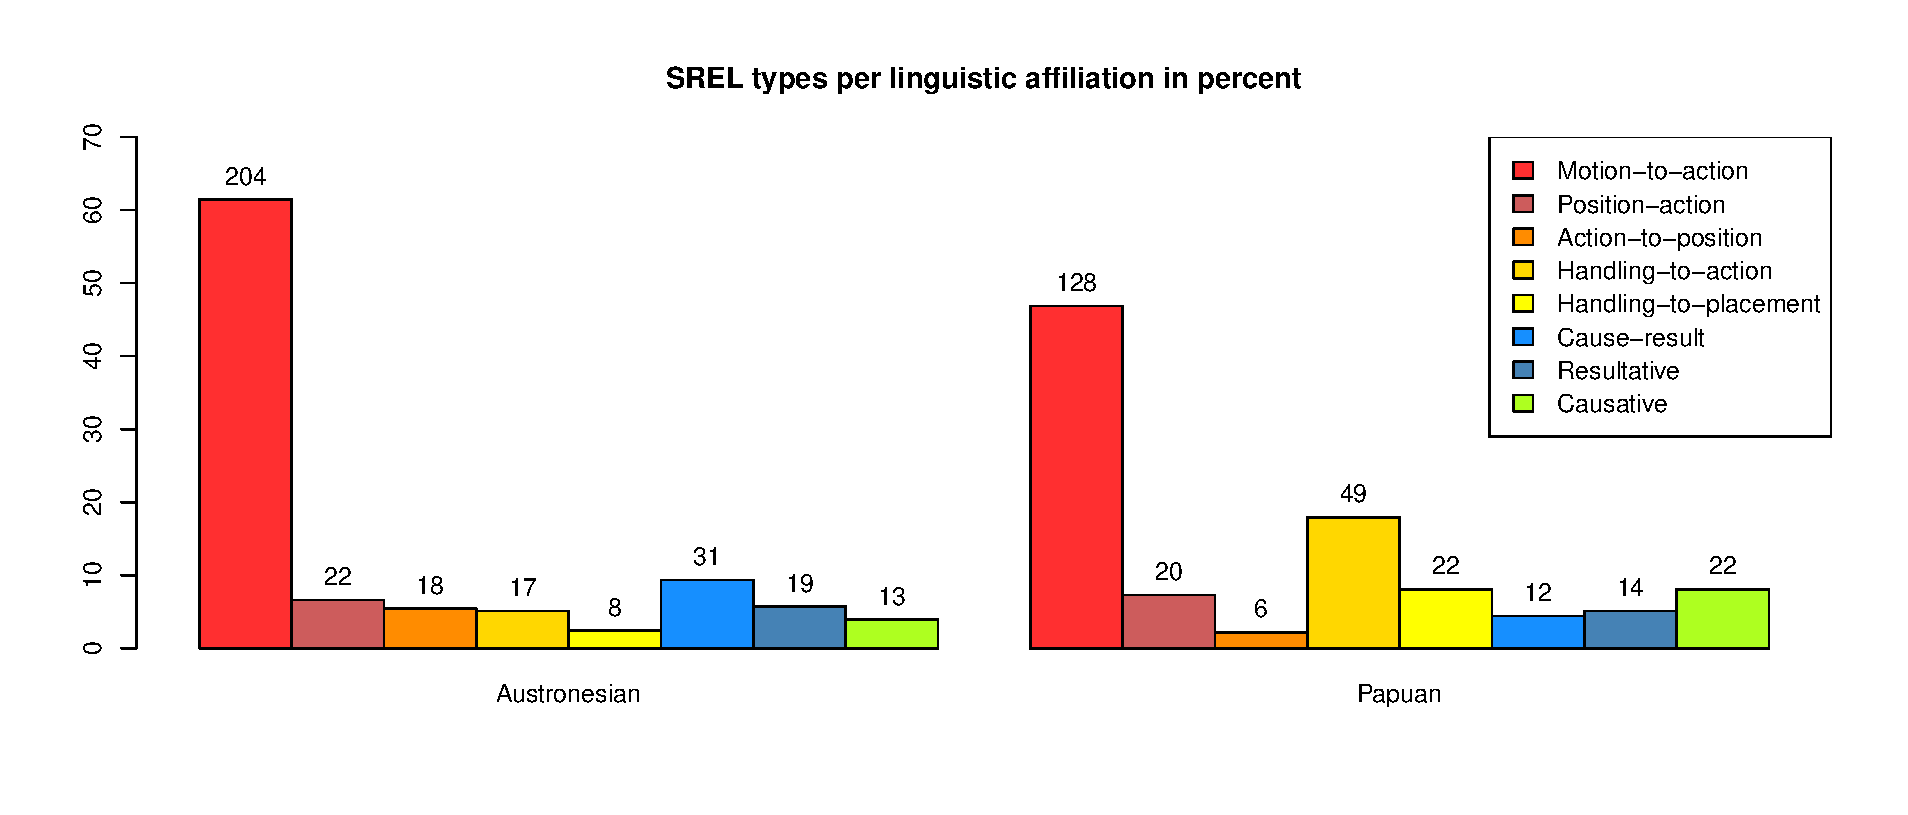
\includegraphics[width=\columnwidth]{figures/SREL_Family.eps}
\caption[SREL types per linguistic affiliation in percent]{SREL types per linguistic affiliation in percent. Numbers on top of the bars refer to the number of observations in the sample.}\label{fig:srel-family}
\end{figure}
\begin{figure}[ht]
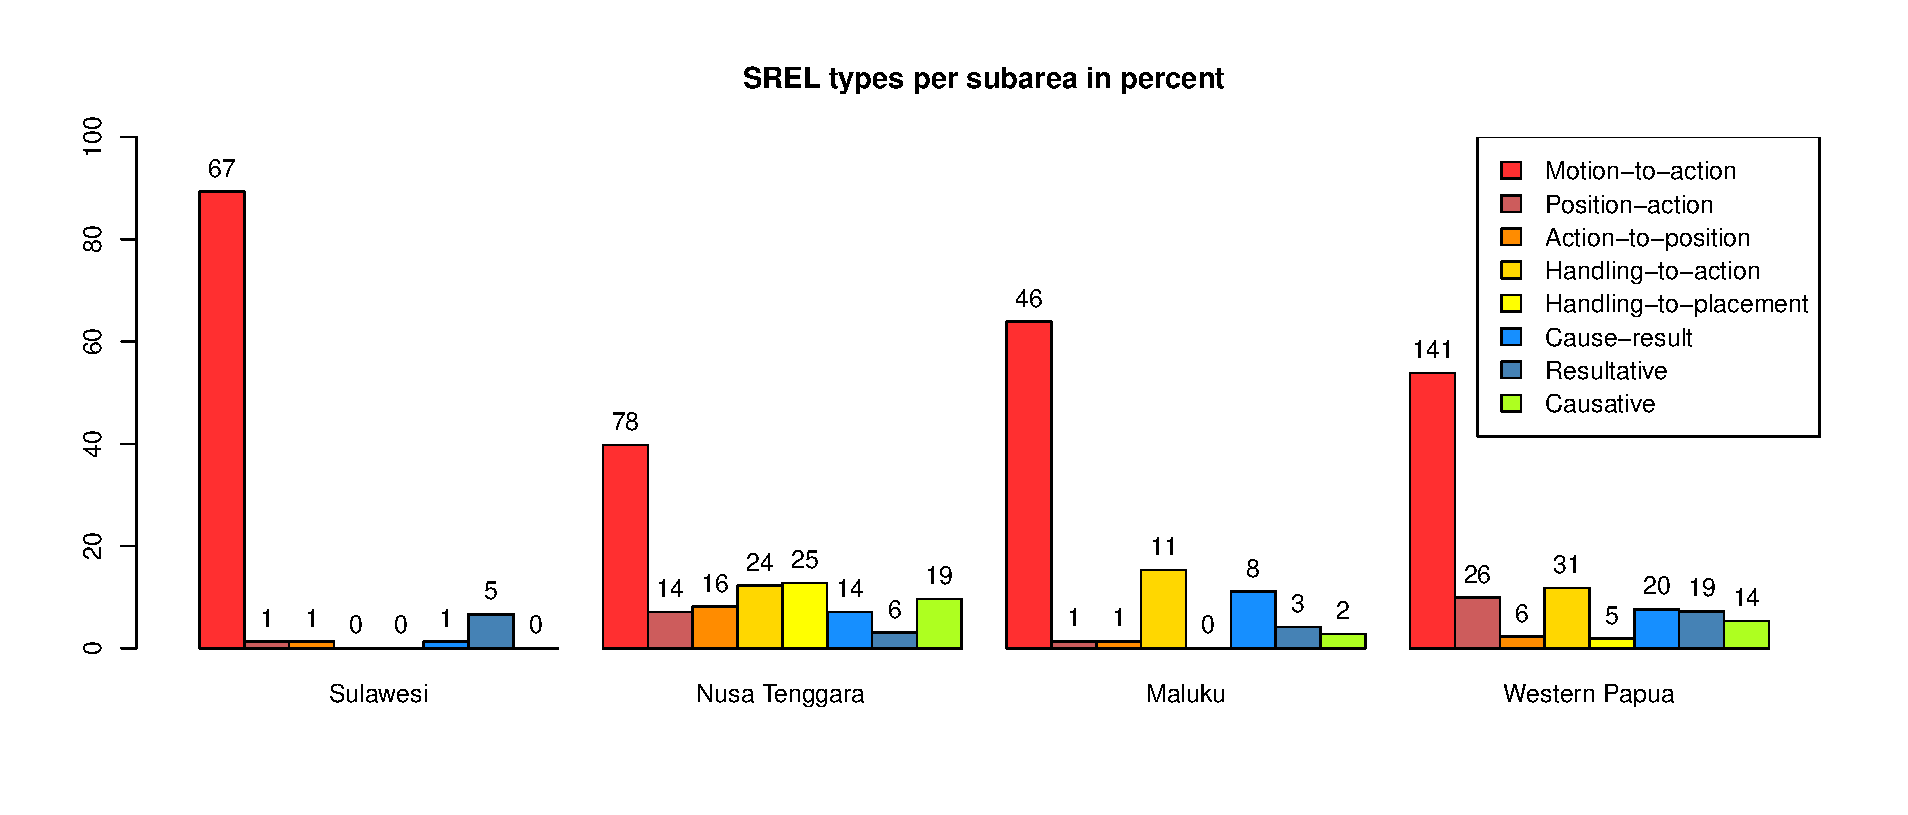
\includegraphics[width=\columnwidth]{figures/SREL_Group.eps}
\caption[SREL types per subarea in percent]{SREL types per subarea in percent. Numbers on top of the bars refer to the number of observations in the sample.}\label{fig:srel-group}
\end{figure}

The areal distribution of SREL constructions seems even more remarkable. The Sulawesi subarea is practically devoid of SRELs, and only exhibits a high use of motion-to-action across all five languages, except Muna (with only two attested examples%; cf. also \tabref{table:srel-language} below
). The only other SREL construction that is in use is resultatives, but they are confined to two of the three south-eastern languages, Tolaki and Tukang Besi. The other three subareas all bear witness to a much higher diversity of SREL constructions. As with the comparison of language family affiliation above, small differences are discernable from \figref{fig:srel-group}. While Nusa Tenggara languages seem to make good use of all other SREL constructions, the Maluku languages appear to lack the two position-marking constructions, as well as handling-to-placement, which seems to be a defining feature of most Nusa Tenggara languages (in the Western Papua group, only Papuan languages show attested examples of this construction). Another minor SREL construction that peaks in the Nusa Tenggara group is action-to-position. In Western Papua, we only have two languages with attested cases, of which all but one are from Wooi. Note that for this construction, both corpus languages, Waima'a and Wooi, contribute the bulk of instances. Another more general feature of the EI data %, as shown by \tabref{table:srel-language}, 
is that most SREL constructions, especially the major ones, clearly show an even distribution among a majority of EI languages. The position-marking constructions, on the other hand, are more unevenly distributed across the sample, and thus warrant a more cautious treatment.

%\begin{table}
%\begin{scriptsize}
%\begin{tabular}{l r r r r r r r r}
%  \lsptoprule
%& \multicolumn{3}{c|}{orientation} & %\multicolumn{2}{c|}{handling} & %\multicolumn{3}{c}{causation} \\
% & {motion-to-action} & {position-action} & %{action-to-position} & {handling-to-action} & {handling-to-placement} & {cause-result} & {resultative} & {causative} \\ 
%  \midrule
%  Muna &   2 &   0 &   0 &   0 &   0 &   0 &   0 &   0 \\ 
%  Pendau &  19 &   0 &   0 &   0 &   0 &   0 &   0 &   0 \\ 
%  Tajio &  18 &   0 &   0 &   0 &   0 &   0 &   0 &   0 \\ 
%  Tolaki &  18 &   1 &   0 &   0 &   0 &   0 &   1 &   0 \\ 
%  Tukang Besi &  10 &   0 &   1 &   0 &   0 &   1 &   4 &   0 \\ \midrule
%  Abui &   9 &   1 &   0 & 4 & 2 & 0 & 0 &   4 \\ 
%  Alorese &  10 &   0 &   0 &   0 &   0 &   0 &   0 &   7 \\ 
%  Bunaq &   1 &   0 &   1 &   0 &   0 &   0 &   2 &   2 \\ 
%  Kaera &   1 &   0 &   0 &   2 &   5 &   0 &   0 &   2 \\ 
%  Kambera &   1 &   1 &   0 &   0 &   0 &   0 &   0 &   0 \\ 
%  Klon &  10 &   0 &   3 &   5 &   6 &   0 &   1 &   0 \\ 
%  Makalero &   3 &   0 &   0 &   2 &   2 &   2 &   0 &   0 \\ 
%  Teiwa &   9 &   9 &   0 &   6 &   1 &   2 &   0 &   2 \\ 
%  Tetun &   6 &   0 &   0 &   3 &   0 &   6 &   3 &   1 \\ 
%  Waima'a &  19 &   1 &   12 &   2 &   8 &   2 &   0 &  0 \\ 
%  Western Pantar &   9 &   2 &   0 &   0 &   1 &   2 &   0 &   1 \\ \midrule
%  Buru & 16  &  0 & 0 & 0  & 0  &  3 & 0  &  2 \\
%  Selaru &   1 &   0 &   0 &   0 &   0 &   1 &   0 &  0 \\ 
%  Taba &   8 &   0 &   0 &   4 &   0 &   3 &   3 &  0 \\ 
%  Tidore & 14 & 1 & 0 & 7  & 0  &  1 &  0 & 0 \\
%  Tobelo &   7 &   0 &   1 &   0 &   0 &   0 &   0 & 0 \\ \midrule
%  Abun &  14 &   0 &   0 &   0 &   0 &   0 &   0 &   1 \\ 
%  Biak &  11 &   5 &   0 &  0 &   0 &   11 &   3 &   1 \\ 
%  Dusner &  10 &   4 &   0 &   1 &   0 &   1 &   0 &   1 \\ 
%  Hatam &  14 &   0 &   0 &   7 &   2 &   0 &   0 &   0 \\ 
%  Inanwatan &   1 &   0 &   1 &   2 &   0 &   0 &   0 &   2 \\ 
%  Maybrat &   6 &   5 &   0 &   1 &   2 &   1 &   3 &   3 \\ 
%  Mor &  22 &   0 &   0 &   0 &   0 &   1 &   0 &   0 \\ 
%  Moskona &   8 &   2 &   0 &   7 &   1 &   2 &   5 &   5 \\ 
%  Mpur &  10 &   0 &   0 &   1 &   0 &   0 &   3 &   0 \\ 
%  Sougb &  12 &   0 &   0 &   5 &   0 &   2 &   0 &   0 \\ 
%  Wooi &  33 &  10 &   5 &   7 &   0 &   2 &   5 &   1 \\ 
%   \midrule
%      Total & 332 & 42 & 24 & 66 & 30 & 43 & 33 & 35 \\
%   \midrule
%\end{tabular}
%\end{scriptsize}
%\caption{Distribution of attested SREL construction types across the EI languages}
%\label{table:srel-language}
%\end{table}

The morphosyntactic patterns found with SREL constructions also return a rather homogeneous picture when compared to the MOD constructions from the last sections. Starting with referentiality values, we find that the values ``A", ``E", and ``X" hardly appear at all in SREL constructions. The dominant pattern for orientation and handling constructions is ``S", while for SRELs denoting causation, the "D" pattern is predominant. Action-to-position MVCs seem to cluster in this regard with causation rather than with orientation, and, as we shall see later, they arguably involve semantics of causation. Head marking in SREL MVCs is also subject to variation across the different constructions. While the ubiquitous motion-to-action constructions may appear in any headedness pattern (both heads marked being the most frequent one, though), the other constructions seem to be more constrained. In most cases, the ``B" pattern is prevalent, followed by ``1" and ``S". However, neither handling construction is attested with a shared affix set (``S"). The less common patterns ``2" and ``N" only occur sporadically with most SRELs. In terms of contiguity, the verbs in SREL constructions are preferentially construed in tight sequence, with two exceptions. In both handling-to-action and handling-to-placement constructions, the value ``1" occurs more frequently than the ``C" value. This reflects the transitive nature of the first verb in such constructions, as the object of the \textsc{handling} verb is typically expressed by a full NP before the following V$_2$, at least in AVO languages.

\begin{table}
\centering
\begin{tabular}{rrrrrr}
  \lsptoprule
Referentiality & S & SO & D & A & X \\ 
  \midrule
  motion-to-action & 326 &   3 &   2 &   1 &   0 \\ 
  position-action &  42 &   0 &   0 &   0 &   0 \\ 
  action-to-position &  11 &   0 &  11 &   0 &   2 \\ 
  handling-to-action &  55 &   9 &   2 &   0 &   0 \\ 
  handling-to-placement &  24 &   5 &   1 &   0 &   0 \\ 
  cause-result &  18 &   6 &  18 &   0 &   1 \\ 
  resultative &   5 &   1 &  26 &   0 &   1 \\ 
  causative &   9 &   0 &  26 &   0 &   0 \\ 
   \midrule
 \\
  \midrule
Headedness & B & 1 & 2 & S & N \\ 
  \midrule
  motion-to-action & 144 &  26 &  24 &   9 &  22 \\ 
  position-action &  23 &   3 &   0 &   1 &   2 \\ 
  action-to-position &   6 &   0 &   0 &   2 &   0 \\ 
  handling-to-action &  32 &   3 &   1 &   0 &   6 \\ 
  handling-to-placement &   5 &   0 &   0 &   0 &   0 \\ 
  cause-result &  14 &  11 &   0 &   1 &   0 \\ 
  resultative &  10 &   7 &   0 &  10 &   0 \\ 
  causative &  10 &   0 &   0 &   3 &   0 \\ 
   \midrule
 \\
  \midrule
Contiguity & W & C & 1 & 2 & 3 \\ 
  \midrule
  motion-to-action &  12 & 261 &  55 &   3 &   1 \\ 
  position-action &   0 &  32 &   9 &   1 &   0 \\ 
  action-to-position &   1 &  17 &   5 &   1 &   0 \\ 
  handling-to-action &   2 &  23 &  35 &   4 &   2 \\ 
  handling-to-placement &   0 &   7 &  18 &   5 &   0 \\ 
  cause-result &   2 &  33 &   7 &   1 &   0 \\ 
  resultative &   0 &  19 &  13 &   1 &   0 \\ 
  causative &   3 &  20 &  12 &   0 &   0 \\ 
   \lspbottomrule
\end{tabular}
\caption[Morphosyntactic properties of SREL constructions]{Morphosyntactic properties of SREL constructions in EI. Table components from top to bottom refer to referentiality (see §\ref{sec:argumentstructure}), headedness (see §\ref{sec:headedness}), and contiguity (see §\ref{sec:contiguity}), respectively. Referentiality values: S = Co-functional (``same subject"), SO = Transitive co-functional (``same subject and object"), D = Switch-function (``Different subject"), A = Participant accumulation, E = Event-to-argument (``Ambient"), X = no interaction, no arguments shared. Headedness values: B = Both verbs marked, 1 = First verb marked, 2 = Second/final verb marked, S = Shared affix set, N = None of the verbs marked. Contiguity values: W = Within word, C = Contiguous verbs 1 = One non-verbal constituent intervening, 2 = Two non-verbal constituents intervening, 3 = Three non-verbal constituents intervening, 4 = Four non-verbal constituents intervening.}
\label{table:SREL_formal}
\end{table}

The subsequent sections turn to the SREL constructions and provide examples.

\subsection{Orientation} \label{sec:orientation}
\subsubsection{Motion-to-action} \label{sec:motion-to-action}

Motion-to-action constitutes the only MVC type found in all EI languages investigated, and can therefore be regarded as the prototypical MVC in Eastern Indonesia. This is a surprising result given that this construction appears not to have received major attention in the serialisation literature. Instances of motion-to-action have two slots, a \textsc{motion} slot followed by an \textsc{action} slot, each of which may be filled recursively with another MVC. \tabref{table:motion-to-action} illustrates the distributional properties of motion-to-action in the EI area.

\begin{table}
\begin{tabular}{ll}
\lsptoprule
Feature&Value\tabularnewline
\midrule
Template&V1 \textsc{motion verb} -- V2 \textsc{action verb}\tabularnewline
No. of attested instances& 332/2146 \tabularnewline
No. of attested languages& 32/32 \tabularnewline
Distribution across areas& \textsc{sul} (5/5), \textsc{nus} (11/11), \textsc{mal} (5/5) \textsc{pap} (11/11) \tabularnewline
Distribution across families& \textsc{pap} (16), \textsc{aus} (16) \tabularnewline
\lspbottomrule
\end{tabular}
\caption[Template and basic distribution of motion-to-action MVCs]{Template and basic distribution of motion-to-action MVCs in the EI sample.}
\label{table:motion-to-action}
\end{table}

The following examples illustrate motion-to-action cases from the different subareas. As can be seen, the motion stage always comes first, and leads up to a second stage in which some action is carried out by the actor. The motion slot in V$_1$ is typically filled by a directed path verb, such as \textsc{come} or \textsc{go} (as in example (\ref{Tajio_18}) from Tajio), but may also host a range of other motion verbs, for instance vertical path verbs (as in example (\ref{Buru_12}) from Buru), punctual contained-path verbs like \textsc{enter} in (\ref{Western_9}) from Western Pantar, or semantically more specific verbs as \textit{mbur} in the Dusner example in (\ref{Dusner_45}) (\textit{mbur} is variously glossed as `leave' or `go home'). The verbs participating in motion-to-action constructions may either all bear inflection (as in the Tajio example), or none of the verb takes inflection (the Western Pantar and Buru cases). In some languages like Hatam, only the motion verb in V$_1$ is inflected. Even rarer is the inflectional pattern found in Inanwatan where the second verb is the locus of inflection, and the motion verb is preposed to it (see also below). Shared affix sets are quite uncommon with motion-to-action, and even languages that allow for this coding type in other MVCs refrain from using it with motion-to-action (for example, Tukang Besi).

\ea \label{Tajio_18}
\langinfo{Tajio}{Austronesian, WMP}{\citealt[294]{mayani2013grammar}}\\
\glll sia’u jo majaok mongulam \\
sia’u jio mV-jaok moN-ulam \\
1\textsc{sg} \textsc{neg} \textsc{st}.\textsc{nrls}-come \textsc{av}.\textsc{nrls}-cure \\
\glft `I will not come to cure (you).’\\ 
\z

\ea \label{Western_9}
\langinfo{Western Pantar}{Papuan, TAP}{\citealt[81]{holton2014western}}\\
\gll wakke bogga gai aname ging aukung banang \\
child young.man 3\textsc{sg}.\textsc{poss} person 3\textsc{pl}.\textsc{act} enter ask \\
\glft `The young man's people go in and ask.'\\ 
\z

\ea \label{Buru_12}
\langinfo{Buru}{Austronesian, CMP}{\citealt[209]{grimes1991buru}}\\
\gll sira te keha baga saka huma lale-n moo \\
3\textsc{pl} \textsc{abil} ascend sleep up house inside-\textsc{gen} \textsc{neg} \\
\glft `They can't go up and sleep inside the [pile] house.'\\ 
\z

\ea \label{Dusner_45}
\langinfo{Dusner}{Austronesian, SHWNG}{\citealt[52]{dalrymple2012}}\\
\glll ndombur na rau ro ran rine ye ndoton e ro \\
ndo-mbur ra rau ro ran ri-ne ye ndo-ton e ro \\
1\textsc{in}.\textsc{pl}-leave move seaward at sago \textsc{evid}-\textsc{dem}.\textsc{prx} \textsc{fill} 1\textsc{in}.\textsc{pl}-sit \textsc{fill} at \\
\glft `We went on seaward to the sago trees where we stayed.'\\ 
\z

It becomes clear from these examples that the action slot does not only permit dynamic verbs. Rather, what seems crucial is that the moving referent is the willful instigator of the action to take place at the place of destination. That is, the stage of sleeping in the Buru example from (\ref{Buru_12}) is planned or intended by the group of referents to take place after they reach the pile house. And in example (\ref{Dusner_45}) from Dusner, the staying is part of the event schema in much the same way, and is interpreted to motivate the change of place denoted by the forerunner motion stage.

Let us now turn to more complex examples. As I said, motion-to-action MVCs appear to allow the construal of stacked MVCs in either of their slots. Example (\ref{Tetun002}) from Tetun Fehan shows a motion complex MVC in initial position followed by a single verb, \textit{hasoru}, in the action slot. Example (\ref{KYO003}) from Klon illustrates the opposite case: Here, the action slot of a motion-to-action construction hosts another MVC (note that Klon has APV word order and places locative verbs in construction-initial position so that the action slot is here filled by a construction [\textsc{locative} \textsc{action}]). Both options of stacked MVCs are attested in a range of EI languages, though not in all. What is licit within a given slot thus seems to be first and foremost a result of language-specific rules.

\ea \label{Tetun002}
\langinfo{Tetun Fehan}{Austronesian, CMP}{\citealt[172]{vanklinken1999grammar}}\\
\gll ha'u k-sai mai k-asoru nia \\
\textsc{1}\textsc{sg} \textsc{1}\textsc{sg}-exit come \textsc{1}\textsc{sg}-meet \textsc{3}\textsc{sg} \\
\glft `I came out and met him.'\\ 
\z

\ea \label{KYO003}
\langinfo{Klon}{Papuan, TAP}{\citealt[148]{baird2008grammar}}\\
\gll hle onon uqlilik, bo leer ga ma, bo waa qad Koilal Marka g-hoi \textbf{qad} amai alol \textbf{mi} \textbf{ted} \\
Kui \textsc{pl} vengeful \textsc{seq} ruler \textsc{3}.\textsc{act} come \textsc{seq} go come Koilal Marka \textsc{3}.\textsc{ug}-order come below harbour be.at sail \\
\glft `The Kui were vengeful so the ruler came, then came and went and ordered Koilal Marka to come sail below in the harbour.'\\ 
\z

Some Papuan languages have only very few or even just one attested example for motion-to-action. This is the case in Bunaq and Inanwatan. The number of attested case remained low even after a search of the appended texts of the respective data sources. We would therefore need to assume that, although motion-to-action construals are probably available in all EI languages one way or another, such construals differ considerably in the extent to which they are used in natural speech. While speakers of some languages put motion-to-action MVCs to good use in all kinds of speech contexts (for instance in Wooi), speakers of other languages like Bunaq or Inanwatan tend not to compress motion and action sequences into the shape of a clause (or better, an IP). The following examples show the only attested cases of motion-to-action for Bunaq and Inanwatan, all of which are but dubious members of motion-to-action. Example (\ref{Bunaq_60}) is the only example that I annotated as a potential case of motion-to-action in Bunaq. It is ambiguous between a translational motion interpretation (keep on going to (the garden) and clear undergrowth) and a grammaticalised aspectual reading (keep on clearing undergrowth), but as the example occurs in \citet[463]{schapper2009bunaq} right after another example with \textit{mal ciluq} that obviously denotes translational motion, I tentatively interpret it as motion-to-action. If this indeed belongs to the group of motion-to-action MVCs, it is one of only a handful of examples in which the order of motion and action is inverted. If SREL MVCs are defined as always retaining the iconicity of the event sequence, then this example would need to be dropped. In the text sample appended to Schapper's grammar I only came across one more utterance that bears a resemblance to motion-to-action. The placement of a comma, however, prevented me from adding (\ref{Bunaq_n1}) to the EI sample. Another feature that would hint at a less tight construal is the use of two different aspectual operators, each targeting one of the verbs. This is unusual even for two-stage MVCs that at times allow the temporal modification of only one event stage (think again of the introductory example (\ref{WMH_Julio_goat099}) from Chapter \ref{ch:sem} where the placement of the aspectual \textit{lo} was right after the motion verb, and not after the whole motion-to-action construction). Example (\ref{Inan_20}), finally, is the only case of motion-to-action that I found in \citet{devries2004}. At the matrix level, two constituents are juxtaposed: \textit{mé-iqo-rita-re} and \textit{mo-wé-tira-rita-i}. The second constituent again forms a MVC, and shows the by-now familiar construal of Inanwatan ``complex phrasal verbs" (cf. \citealt[57]{devries2004}) with a bare verb (in this case the motion verb) preposed to an inflected V$_2$ that takes an object indexing prefix and a set of suffixes denoting TAM and subject number and gender. Note that although Inanwatan is strictly AOV, the order of the verbs still follows the temporal order of event stages.

\ea \label{Bunaq_60}
\langinfo{Bunaq}{Papuan, TAP}{\citealt[463]{schapper2009bunaq}}\\
\gll u t-ul mal ciluq \\
undergrowth 3\textsc{inan}-pull go rest \\
\glft ‘(They) keep going to clear undergrowth.’\\
\z

\ea \label{Bunaq_n1}
\langinfo{Bunaq}{Papuan, TAP}{\citealt[512]{schapper2009bunaq}}\\
\gll rebel si, g-ota gie \\
descend \textsc{rls} 3\textsc{an}-stab \textsc{prosp} \\
\glft ‘(They) would go down to stab (them).’\\ 
\z

\ea \label{Inan_20}
\langinfo{Inanwatan}{Papuan, SBH}{\citealt[85]{devries2004}}\\
\gll sudah mai mé-iqo-rita-re mo-wé-tira-rita-i, tígo mao-go mé-ra-rita-i \\
so this.\textsc{f} 3\textsc{sg}-put.down-\textsc{dur}-\textsc{pst}.\textsc{pl} come-3\textsc{sg}-take-\textsc{dur}-\textsc{pst}.\textsc{pl} so wife-\textsc{circ} 3\textsc{sg}-take-\textsc{dur}-\textsc{pst}.\textsc{sg}.\textsc{m} \\
\glft `So they put her down and he came and took her to become his wife.'\\ 
\z

\subsubsection{Position-action}\label{sec:position-action}

Position-action MVCs combine a posture verb in V$_1$ with an action verb in V$_2$. It is the only construction in the SREL constructional family that does not produce a reading of two successive spatio-temporal stages, but invokes an interpretation of two events going on at the same time. The acting participant assumes a certain position (and, at least in case of \textsc{sit} and \textsc{stand} verbs, invests energy to maintain this position), while performing some action at the same time. I regard such construals as two-stage nonetheless with the only difference that the event stages overlap in space and time. The question whether or not two situations that overlap in space and time constitute one and the same event has been raised in formal semantics, but a one-event conclusion has been dismissed as too narrow a definition of eventhood (see e.g. \citealt{maienborn2005limits} for discussion). Therefore we may assume that two event arguments, licensed by two LLEs, may refuse merging although they are interpreted as happening at the same time and place. As \tabref{table:position-action} illustrates, position-action MVCs are only sparsely distributed over the EI region (with attested examples in 12 languages). Both Sulawesi and Maluku hardly show any usage at all (one attested example each), and in the two other subareas, it is only some languages that make regular use of it.

\begin{table}
\begin{tabular}{ll}
\lsptoprule
Feature&Value\tabularnewline
\midrule
Template&V1 \textsc{posture verb} -- V2 \textsc{action verb}\tabularnewline
No. of attested instances& 42/2146 \tabularnewline
No. of attested languages& 12/32 \tabularnewline
Distribution across areas& \textsc{sul} (1/5), \textsc{nus} (5/11), \textsc{mal} (1/5) \textsc{pap} (5/11) \tabularnewline
Distribution across families& \textsc{pap} (6), \textsc{aus} (6) \tabularnewline
\lspbottomrule
\end{tabular}
\caption[Template and basic distribution of position-action MVCs]{Template and basic distribution of position-action MVCs in the EI sample.}
\label{table:position-action}
\end{table}

Here are some typical examples from languages with more than one attested example: Teiwa in the Nusa Tenggara group, Maybrat and Wooi in the Western Papua group. According to \tabref{table:SREL_formal} from §\ref{sec:stage-relating}, prototypical position-action constructions have shared subject arguments (``S"), both verbs are inflected (``B"), and the verbs are placed adjacent to each other (``C"). In case V$_2$ has a transitive verb with a full object NP, this would lead in AOV languages to an NP placement between the position verb and the action verb, as in example (\ref{Teiwa_24}) from Teiwa. There are three posture verbs that may be found in the position slot: \textsc{sit} verbs, as in example (\ref{Teiwa_24}) from Teiwa, and \textsc{stand} verbs, as in (\ref{Maybrat_75}) and (\ref{WBW016}), occur most frequently, but occasional examples with \textsc{lie} verbs are attested for Biak, Moskona, and Wooi (all belonging to the Western Papua subarea). While the Teiwa example illustrates a basic positon-action construction consisting of just two verbs, the examples from Maybrat and Wooi both show complex construals in which the action slot hosts another MVC. In example (\ref{Maybrat_75}) we encounter a three-verb string, denoting three event stages: a position stage, a handling stage, and, finally, a placement stage. As handling-to-placement MVCs recur in a number of languages, I propose that they constitute a stage-relating MVC type of their own (see §\ref{sec:handling-to-placement} below). In this case, it seems as if the action slot of a position-action construction is filled with a handling-to-placement MVC. This is the only way the string can be resolved without violating the handling-to-placement template that requires a handling verb in V$_1$. The Wooi case in (\ref{WBW016}) illustrates another stacked MVC with a position-action construction at the matrix level. Here, it is a direction complex MVC, consisting of three verbs \textit{hayo} `watch', \textit{tuva} `go.after' and \textit{ra} `go', that enters the action slot. I have not come across MVCs filling the position slot of position-action constructions, though.\footnote{The only potential combination that would not be semantically odd is, I think, a locative case-marking MVC embedded into the position slot of position-action, thus yielding something like \textit{Jones \textbf{sit} \textbf{be} in bathroom \textbf{butter} toast}. Such a combination, however, is not attested in the sample. Another potential combination, action-to-position plus position-action, seems to be at odds with the constructional meanings, as the former mostly denotes an object that is brought into a certain position by some action. Action-position-action would then involve a participant in object function that is placed somewhere, and only then performs (now in subject function) some action - a setting that would be quite uncommon by all accounts.}

\ea \label{Teiwa_24}
\langinfo{Teiwa}{Papuan, TAP}{\citealt[309]{klamer2010grammar}}\\
\gll a yix-in si, ga-gasqai ga'an atab un mis-an qar tapan pati \\
3\textsc{sg} descend-\textsc{rls} \textsc{sim} 3\textsc{sg}-sister 3\textsc{sg} truly \textsc{cont} sit-\textsc{rls} rice pound \textsc{prog} \\
\glft `While he went down, his sister [was] actually still sitting pounding rice.'\\ 
\z

\ea \label{Maybrat_75}
\langinfo{Maybrat}{Papuan, isolate}{\citealt[215]{dol2007grammar}}\\
\gll y-ros y-o y-ati ara a \\
3\textsc{m}-stand 3\textsc{m}-take 3\textsc{m}-put.in.ground tree \textsc{int} \\
\glft 1. `Does he stand and take and put the sticks into the ground?' \\ 2. `He stands and takes (the sticks), but should he put them into the ground (or should he do something else with them)?'\\
\z

\ea \label{WBW016}
\langinfo{Wooi}{Austronesian, SHWNG}{WBW\_pear\_Agus}\\
\glll henda kutua mara trus ce heyo tuva hnia ra mara \\
he-ra kutu-a mara trus $<$i$>$tera $<$i$>$hayo tuva hnia ra mara \\
\textsc{3}\textsc{pl}-go cut-\textsc{obj}.\textsc{nsg} \textsc{seq} then $<$\textsc{3}\textsc{sg}$>$stand $<$\textsc{3}\textsc{sg}$>$watch go.after \textsc{3}\textsc{pl} go \textsc{seq} \\
\glft `He stood and watched them passing as they went past him.'\\ 
\z

Example (\ref{Maybrat_75}) above also illustrates another property of position-action in Maybrat. If an interrogative marker is added to the construction, it may either target the whole matrix MVC, or just the last event stage that is adjacent to the clause-final marker. This behaviour thus mirrors the criterion of partial temporal modification that I suggested in §\ref{sec:criteria_mvcs} to be a defining characteristic of SRELs.

One example with a reversed order action -- position was found in Teiwa as well. I suppose that \textit{ga-boxan tas} in (\ref{Teiwa002}) can be considered a lexicalised combination rather than a regular example of position -- action.

\ea \label{Teiwa002}
\langinfo{Teiwa}{Papuan, TAP}{\citealt[314]{klamer2010grammar}}\\
\gll rai na-soi ga-kamadal ga-boxan tas \\
king \textsc{1}\textsc{sg}-order \textsc{3}\textsc{sg}-belt \textsc{3}\textsc{sg}-guard stand \\
\glft `The king ordered me to guard his belt.'\\ 
\z

\subsubsection{Action-to-Position}\label{sec:action-to-position}

Action-to-position instances consist of an action stage followed by a positional stage. The second stage may either be a posture verb, specifiying the spatial alignment of some object, or a stative positional verb, stressing a non-dynamic resultant phase after the action stage has come to an end. Action-to-position is confined to only 24 cases from seven languages, from all subareas. Its distribution is hard to trace as there are so little data, but it seems that, by looking at the data points per language, the number of occurrences can be increased by searching through larger language corpora, as the number of cases from Waima'a and Wooi illustrates. The frequency of action-to-position in EI natural speech data seems at any rate to be rather low. \tabref{table:action-to-position} presents the basic numbers.

\begin{table}
\begin{tabular}{ll}
\lsptoprule
Feature&Value\tabularnewline
\midrule
Template&V1 \textsc{action verb} -- V2 \textsc{posture/positional verb}\tabularnewline
No. of attested instances& 24/2146 \tabularnewline
No. of attested languages& 7/32 \tabularnewline
Distribution across areas& \textsc{sul} (1/5), \textsc{nus} (3/11), \textsc{mal} (1/5) \textsc{pap} (2/11) \tabularnewline
Distribution across families& \textsc{pap} (4), \textsc{aus} (3) \tabularnewline
\lspbottomrule
\end{tabular}
\caption[Template and basic distribution of action-to-position MVCs]{Template and basic distribution of action-to-position MVCs in the EI sample.}
\label{table:action-to-position}
\end{table}


Action-to-position MVCs fall into two subtypes, as stated above: (i) action-to-posture, and (ii) action-to-positional state. For lack of data, I tentatively included both subtypes under one constructional schema, but they may in fact constitute related but different constructions. The former variant is attested in most of the languages that have action-to-position. Consider the following examples. In example (\ref{Waimaqa_65}) from Waima'a and example (\ref{Tobelo_20}) from Tobelo a participant is pulled into upright position. The construction involves a verb of pulling complemented by a \textsc{stand} verb in V$_2$. Example (\ref{Wooi_86}) from Wooi illustrates another posture verb in V$_2$. Here, the object referent is brought into a horizontal lying position (\textsc{lie} verbs are in fact only attested in Wooi). Note that the referential expression of such construals needs to have a shift in syntactic function: the direct object of V$_1$ is to become the subject of V$_2$, as exemplified by the Wooi case in (\ref{Wooi_86}). What is interesting with the first two examples is that although such a reference shift arguably takes place on the logical-conceptual level, the formal encoding of the referential expressions does not exactly follow this shift. Rather, in the Waima'a case, we observe a referential shift from the boy's arm (the object of V$_1$) to the boy now being understood as the referent that is moved to a standing position (since it is not just the boy's arm that is supposed to stand as a result of the event). A similar shift takes place in the Tobelo example. Here, the referent being pulled up is expressed by a third person object prefix on the first verb, yet on the posture verb the same referent is referred to with a second person subject indexer. Such person shifts are not uncommon in the languages of the Melanesian region, and are used to highlight prominent parts of natural speech contexts, for instance in story narration (see \citealt{margetts2015person} for a recent account of person shifts in Saliba-Logea). Discourse structure in such contexts shapes the grammatical expression of referents. This is another interesting case of unreliable morphology where the formal encoding of referential expression does not lead to a disambiguation of internal MVC structure.

\ea \label{Waimaqa_65}
\langinfo{Wama'a}{Austronesian, CMP}{pear\_Bendita 030}\\
\gll sik ale'e askai ke lime nini nhii ulo \\
grab child male \textsc{dem} arm \textsc{poss} stand already \\
\glft `They grabbed the boy's hand (to help him) get
up.'\\ 
\z

\ea \label{Tobelo_20}
\langinfo{Tobelo}{Papuan, NH}{\citealt[63]{holton2003tobelo}}\\
\gll t-a-ika t-i-tauru no-maoko la no-ma-tagi \\
1-vf-\textsc{all} 1-3\textsc{m}-pull 2-stand \textsc{conj} 2-\textsc{refl}-walk \\
\glft `I pulled him up so that he could walk' (lit. I pull him you stand...)\\ 
\z

\ea \label{Wooi_86}
\langinfo{Wooi}{Austronesian, SHWNG}{midwife\_traditional\_medicine}\\
\glll heton via topi ning ma heteng kepan \\
he-ong $<$i$>$va topi ning ma he-eng kepang \\
3\textsc{pl}-put $<$3\textsc{sg}$>$lie like this \textsc{top} 3\textsc{pl}-sleep overlap \\
\glft `Preparing it (the leaves) like this they sleep on it.' (lit. putting it lie like this, they sleep on it) \\ 
\z

As \textit{va(ta)} `lie' may also convey durative semantics in Wooi, the Wooi case in (\ref{Wooi_86}) straddles the dividing line between both subtypes of action-to-position. This becomes obvious in examples such as the following where the pig assumes a lying position only as a result of its being dead. In my understanding, the main semantic contribution of \textit{vata} in such cases is that it translates into an aspectual notion of durative resultant state, something like `die and remain (lying) there for some time'.

\ea 
\langinfo{Wooi}{Austronesian, SHWNG}{MANTERA\_magic\_charms}\\
\glll asurang vat keria viata \\
asurang vati $<$i$>$karia $<$i$>$vata \\
pig \textsc{det}:\textsc{sg} $<$3\textsc{sg}$>$-die $<$3\textsc{sg}$>$-lie \\
\glft `(After slashing it with a machete) the pig dies.'\\ 
\z

Similar cases in which V$_2$ introduces some kind of stative resultant stage are found in Waima'a. Consider example (\ref{WMHP136}) below with a \textsc{stay} verb in final position, probably specifying that the placement of the basket on the bicycle has been successfull, and that it would remain there.

\ea \label{WMHP136}
\langinfo{Waima'a}{Austronesian, CMP}{pear\_Carlito 140}\\
\gll ne boten mai tese hite n'au biskalta oon \\
\textsc{3}\textsc{sg} basket come place \textsc{ptl} stay bicycle above \\
\glft `His basket, (they) came putting it onto (his) bicycle.' \\ 
\z

There is a very small number of further constructions that seem similar to action-to-position constructions, but have a rather specific stative verb in V$_2$ position. Example (\ref{MOSK001}) from Moskona is such a case. More data would be helpful in order to gain a clearer picture on such constructions.

\ea \label{MOSK001}
\langinfo{Moskona}{Papuan, EBH}{\citealt[295]{gravelle2010grammar}}\\
\gll ofa eyta meber efifr-ef \\
s/he take shelf level-near \\
\glft ‘He made the shelf [so] it is level.’\\ 
\z

\subsection{Handling}

In the last sections, we have seen stage-relating constructions that in some way or another contribute information on the spatial setting of events. Motion-to-action motivates a shift from one location to another by entailing that the moving actor is moving with some clear intention. Motion-to-action thus helps shift the discourse scene in story telling. SREL constructions involving positional verbs provide information on stative spatial orientation of some participant, either specifying the body posture of some acting participant, or the resting position of some manipulated object. 

Handling constructions are quite different and focus on the manual manipulation of objects, and what actions follow from them. Just as in orientation SRELs, there is normally a strong implication of intentional acting entailed in handling SRELs. I distinguish between two constructions: Handling-to-action and handling-to-placement. 

\subsubsection{Handling-to-action} \label{sec:handling-to-action}

Handling-to-action combines an event stage of manual object handling with a subsequent action stage. Prototypical instances are combinations of a \textsc{take} verb followed by some dynamic action verb in V$_2$. Handling-to-action is the secondmost frequent SREL construction found in the EI sample after motion-to-action. Its distribution seems limited to Nusa Tenggara, Western Papua, and parts of the Halmahera archipelago. In both Nusa Tenggara and Western Papuan languages, the construction occurs in most languages of the sample, though its distribution is skewed towards Papuan languages. \tabref{table:handling-to-action} presents the distributional numbers.

\begin{table}
\begin{tabular}{ll}
\lsptoprule
Feature&Value\tabularnewline
\midrule
Template&V1 \textsc{handling verb} -- V2 \textsc{action verb}\tabularnewline
No. of attested instances& 66/2146 \tabularnewline
No. of attested languages& 17/32 \tabularnewline
Distribution across areas& \textsc{sul} (0/5), \textsc{nus} (7/11), \textsc{mal} (2/5) \textsc{pap} (8/11) \tabularnewline
Distribution across families& \textsc{pap} (12), \textsc{aus} (5) \tabularnewline
\lspbottomrule
\end{tabular}
\caption[Template and basic distribution of handling-to-action MVCs]{Template and basic distribution of handling-to-action MVCs in the EI sample.}
\label{table:handling-to-action}
\end{table}

Handling-to-action MVCs conform to the dominant headedness pattern in that both verbs inflect for verbal categories (disregarding the cases of unreliable morphology in Nusa Tenggara), but they slightly deviate in the other two morphosyntactic categories, referentiality and contiguity. As opposed to most other MVCs, handling-to-action MVCs predominantly have one constituent placed between their verbs. This is typically the direct object NP of the handling verb. In terms of referential interaction, one might expect the number of ``SO" cases (that is, the verbs share subject \emph{and} object) to be quite high because taking something and manipulating it would require such a referential coding. Yet, \tabref{table:SREL_formal} from §\ref{sec:stage-relating} reveals that only a small fraction of cases indeed shows "SO" referential interaction. Most cases exhibit the much more common pattern ``S" where the subject but not the object is shared among the verbs. This is due to the fact that in most instances of handling-to-action, the handling verb introduces an object referent that is then understood as the instrument rather then the theme of the action denoted by the second verb. 

This brings up a further problem: how to distinguish between two-stage handling-to-action MVCs on the one hand, and one-stage instrumental case-marking MVCs on the other. A thorough testing would necessarily involve the criteria sketched in §\ref{sec:criteria_mvcs}. As this was not always possible, I assumed all instances in which \textsc{take} verbs (or related verbs of handling) in V$_1$ combine with verbs denoting manual action to be two-stage MVCs rather than modifying MVCs. This was backed by two assumptions: first, grammaticalised instrument-marking MVCs would probably also comprise cases of rather abstract instrument assignments with concrete manual action being semantically odd. However, all retrieved cases of handling-to-action still denote concrete manual action. And second, no change in constituent order was detected, also pointing to the conclusion that handling-to-action rather constitutes a two-stage event schema, and is constrained by the principle of temporal iconicity. Note that the cases of instrument MODs, as discussed in §\ref{sec:case-marking}, do show variable constituent order, and other properties that lend themselves to an analysis as somewhat grammaticalised instrument-marking constituent.

Let us now first have a look at this major group of instrument-introducing constructions. Consider the following examples. Example (\ref{Abui_103}) from Abui is a prototypical handling-to-action construction, with a \textsc{take} verb in V$_1$ and a subsequent action stage. The theme object of \textit{mi} is interpreted as the instrument that is used to perform the action of cutting wood (note that \textit{kawen} is moved here to a clause-initial focus position). In (\ref{Klon_87}) from Klon, a similar construal is used, but the verb translates as holding, not taking. I am assuming for the time being that such MVCs still form two-stage event construals (either by denoting a precursor stage to obtain the instrument, or in the sense of overlapping stages, as in the position-action construction discussed in §\ref{sec:position-action}). Example (\ref{Hatam_30} from Hatam is a similar case from the Western Papua subarea.

\ea \label{Abui_103}
\langinfo{Abui}{Papuan, TAP}{\citealt[386]{kratochvil2007grammar}}\\
\gll kawen ama mi bataa tukong \\
machete person take wood cut \\
\glft `With machete one cuts wood.'\\ 
\z

\ea \label{Klon_87}
\langinfo{Klon}{Papuan, TAP}{\citealt[146]{baird2008grammar}}\\
\gll gi-doqom ge eneem biasa ini puin iwi we~wei\\
3\textsc{poss}-grandfather 3\textsc{poss} tall.grass usual 3\textsc{nsg} hold house \textsc{rdp}~roof\\
\glft `They usually use his grandfather's tall grass to roof houses.'\\ 
\z

\ea \label{Hatam_30}
\langinfo{Hatam}{Papuan, Hatam-Mansim}{\citealt[101]{reesink1999grammar}}\\
\gll dani di-ba singau riu nab \\
I 1\textsc{sg}-take knife pierce pig \\
\glft `I pierced the pig with a knife.'\\ 
\z

Example (\ref{Hatam_30}) above is in fact not the only way to construe instrument-introducing MVCs in Hatam. In order to explicitly track the instrument argument, an instrument prefix may be used on the second verb. Here is another example from Hatam, showing the use of two homophonous, possibly related, prefixes. The instrument \textit{bi} denotes that the theme object of the preceding verb is interpreted as the instrument of the verb \textit{bi-} is attached to. The second \textit{bi-}, on the other hand, marks purposive relations between two predicates. Note that the placement of the subject indexers distinguishes both prefixes, as the former stands between the indexer and the verb root, while the latter precedes both indexer and verb root.

\ea 
\langinfo{Hatam}{Papuan, Hatam-Mansim}{\citealt[101]{reesink1999grammar}}\\
\gll yoni i-ba micim i-bi-dat dani bigom bi-di-mai \\
they 3\textsc{pl}-take spear 3\textsc{pl}-\textsc{ins}-pierce I almost \textsc{purp}-1\textsc{sg}-die \\
\glft `They almost killed me with their spear(s).'\\ 
\z

Turning to the second group of handling-to-action cases, we can see that there is hardly any difference in construal, at least if the language in question does not overtly mark instruments, as we have seen in the Hatam case above. Take example (\ref{Kaera_7}) from Kaera as an illustration.

\ea \label{Kaera_7}
\langinfo{Kaera}{Papuan, TAP}{\citealt[136]{klamer2014kaera}}\\
\gll gang g-iya-t gang ge-sil tuning met or-i sei \\
3\textsc{sg} 3\textsc{sg}-go.down-\textsc{ipfv} 3\textsc{sg} 3\textsc{sg}-rope placenta take hang-\textsc{prfv} \textsc{compl} \\
\glft `Giving birth, she took his umbilical cord [and] hung [it up].'\\ 
\z

Handling-to-action constructions may in some languages be further extended by an in-between motion slot, resulting in a sequence \textsc{handling - motion - action}. Consider the following example from Teiwa where the motion verb \textit{ma} intervenes between the handling verb and the action verb. In most instances of such inserted motion stages, it is not clear whether there really is an event of translational motion involved.

\ea 
\langinfo{Teiwa}{Papuan, TAP}{\citealt[317]{klamer2010grammar}}\\
\gll ped mat ma man taxar \\
machete take come grass cut \\
\glft `Cut the grass with a machete.'\\ 
\z

In these languages, one sometimes also finds bare \textsc{motion - action} sequences that nevertheless translate into handling-to-action events. In the following example from Western Pantar, the construction transports a grammaticalised meaning of obtaining and transfering an object to some recipient. This is not, of course, to mean that the banana is the moving participant that surrenders itself to the recipient (in fact, it still needs to be licensed by some transitive verb, which is an elided initial \textsc{take} verb). \citet{klamer2012development}, in a paper on give-constructions in the TAP languages, also arrive at the conclusion that such sequences constitute grammaticalised variants of the full templates (elided handling verbs also appear in handling-to-placement, see next section).

\ea 
\langinfo{Western Pantar}{Papuan, TAP}{\citealt[186]{klamer2012development}}\\
\gll nang maggi ma ga-nia \\
\textsc{1}\textsc{sg} banana come \textsc{3}\textsc{sg}-give \\
\glft ‘I give a banana to him.’\\ 
\z

\subsubsection{Handling-to-placement} \label{sec:handling-to-placement}
In the previous section we have seen examples of a SREL construction in which a handling slot combines with an action slot. Some languages, in particular the \textsc{TAP} languages, show a closely related construction consisting of a handling verb followed by a placement verb. As with handling-to-action, particularily in the Nusa Tenggara subarea, an optional motion stage may intervene between the handling stage and the placement stage, that is, producing an event line of an actor handling some object, going somewhere (with it), and placing it somewhere or giving it to somebody. Such construals are reminiscent of transport complexes on the one hand (\textsc{take} plus \textsc{go} as on-stage motion complex MVCs), and of motion-to-action SRELs (\textsc{go} plus \textsc{action}) on the other. However, in most of these cases, there is hardly translational motion encoded in the sense that there is really a change of location involved. It is this difference that, I want to argue, prevent handling-(motion)-placement from being analysed as combinations of the aforementioned MVC types.

Handling-to-placement is strongly associated with Papuan languages in the Nusa Tenggara subarea. The only Austronesian language contributing attested cases is Waima'a. \tabref{table:handling-to-placement} illustrates the basic numbers on its distribution.

\begin{table}
\begin{tabular}{ll}
\lsptoprule
Feature&Value\tabularnewline
\midrule
Template&V1 \textsc{handling verb} -- V2 \textsc{placement verb}\tabularnewline
No. of attested instances& 30/2146 \tabularnewline
No. of attested languages& 10/32 \tabularnewline
Distribution across areas& \textsc{sul} (0/5), \textsc{nus} (7/11), \textsc{mal} (0/5) \textsc{pap} (3/11) \tabularnewline
Distribution across families& \textsc{pap} (9), \textsc{aus} (1) \tabularnewline
\lspbottomrule
\end{tabular}
\caption[Template and basic distribution of handling-to-placement MVCs]{Template and basic distribution of handling-to-placement MVCs in the EI sample.}
\label{table:handling-to-placement}
\end{table}

Prototypical cases of handling-to-placement are used to encode three participant events involving the transfer of something to someone. As ditransitive verbs seem to be rare in the languages of Nusa Tenggara, a handling verb is combined with a \textsc{give} verb in order to encode the transfer of some object from one participant to the other. \citet{klamer2012development} report on give-constructions in TAP languages. There are three constructions available: biclausal construals with a junctor placed between the verbs, serial verb constructions withouth a junctor, and particle-verb combinations \citep{klamer2012development}. The serial verb construction consists of a \textsc{take} verb that introduces a theme argument (the object transferred), and a \textsc{give} verb that licenses the recipient argument. Both T and G are placed in preverbal position as the TAP languages are mostly AOV. Consider the following examples. The first example is from Kaera, and illustrates a construction involving a \textsc{take} verb, a \textsc{give} verb, and a locative element \textit{mi} in-between the verbs. This is probably related to other traces of \#mai `come' in neighbouring TAP languages, and could have originated as a full motion verb. \citet{klamer2012development} point out that such motion verbs appear in many such give-constructions throughout the TAP area, and sometimes they even head a construction with the initial \textsc{take} being elided (see below for examples). Example (\ref{Makalero_6}) is from Makalero and shows a similar construal. We have already discussed the light verb behaviour of \textit{mei} in Makalero that is frequently used to introduce a further argument in case the argument slots of the main verb are already taken. Here, \textit{mei} appears to act like a full-fledged \textsc{take} verb and combines with \textit{kini} to encode an object transfer. What is of particular interest in (\ref{Makalero_6}) is that the second stage, the giving, is repeated in order to denote two different giving events. The \textsc{take} verb obviously does not need to be repeated. This suggests that the handling-to-placement construction is not as tightly construed in Makalero as, say, motion complex MVCs with two motion verbs merging part of their LLEs. Both event stages thus still possess a certain inedependence. Note, however, that neither of the two Makalero linkers, \textit{=ni} nor \textit{=si}, is employed in this construction, although they frequently surface in other contexts. The third example in (\ref{Maybrat_77}) is from Maybrat and shows that handling-to-placement is also found in the Western Papuan group, albeit just in weak traces. As with position-action, handling-to-placement in Maybrat can have interrogative scope over the whole construction, or just on the final constituent. This supports the grouping of both constructions under the label stage-relating, at least for Maybrat. 

\ea 
\langinfo{Kaera}{Papuan, TAP}{\citealt[140]{klamer2014kaera}}\\
\gll xabi mampelei utug met mi kunang masik namung gu gi-ng \\
then mango three take \textsc{loc} children male \textsc{pl} that 3\textsc{pl}-give \\
\glft `Then takes three mangos to give to the children.'\\ 
\z

\ea \label{Makalero_6}
\langinfo{Makalero}{Papuan, TAP}{\citealt[116]{huber2011}}\\
\gll Ani he’ul=afta ho’o mei ni-nana=raa meih=ee kini ni-noko=raa meih=ee kini \\
1\textsc{sg} full=\textsc{cond} some take \textsc{refl}-elder.sibling.\textsc{pl} two.\textsc{hum}=\textsc{def} give.to.3 \textsc{refl}-younger.sibling=\textsc{pl} two.\textsc{hum}=\textsc{def} give.to.3 \\
\glft ‘If I was full, I gave some to my two elder siblings and to my two younger
siblings.’ \\ 
\z

\ea \label{Maybrat_77}
\langinfo{Maybrat}{Papuan, isolate}{\citealt[215]{dol2007grammar}}\\
\gll n-o tapak n-e ait a \\
2-take tobacco 2-give 3\textsc{m} \textsc{int} \\
\glft 1. `Will you take the tobacco and give it to him?' \\ 2. `You take the tobacco, but will you give it to him, or will you do something else with it?' \\ 
\z

A second group of cases does not feature a \textsc{give} verb in final position, but rather a verb of putting or placing the object somewhere. Although this group may alternatively be analysed as another instance of handling-to-action, I found them to be conceptually close to the instances of handling-to-placement introduced above, in that they also constitute a transfer event. A key difference is that the transfer is not directed at a human referent but at a place. Consider the following example from Waima'a, combining a \textsc{take} verb with a \textsc{put} verb in much the same way as the previous examples with a \textsc{give} verb in final position. Note that the placement of the aspectual \textit{lo}, which is normally predicate-final in Waima'a, hints at the two-stage nature of the construction.

\ea \label{WMHP058}
\langinfo{Waima'a}{Austronesian, CMP}{pear\_Santina 140}\\
\gll se wuruo kholi lo kai-wuo thau la bote lale \\
one \textsc{clf}-two pick.up \textsc{asp} fruit put \textsc{loc} basket inside \\
\glft `Two of them pick up the fruits (and) put (them) inside the basket.'\\ 
\z

As I said earlier, in some examples a motion slot intervenes and separates both event stages by denoting what looks like a displacement of a theme object. The Klon example below illustrates a typical template.

\ea 
\langinfo{Klon}{Papuan, TAP}{\citealt[144]{baird2008grammar}}\\
\gll pi méd ma bokor hok mi hos \\
\textsc{1}\textsc{nsg}.\textsc{in}.\textsc{act} take come bowl small.basket be.at place \\
\glft `(This fruit), we bring (it) and place (some) in a bowl or small basket.'\\ 
\z

In some cases the relation between the motion verb and the surrounding verbs remains ambiguous, suggesting an alternative analysis as MVC embedding. Example (\ref{WMHP117}) from Waima'a shows a surface string of a handling verb followed by a deictic motion verb and a placement verb. Here, the context (and the translation given) suggests an analysis as a direction complex  (lift come = lift towards the narrative origo taken by the narrator), nested in an action-to-placement sequence. Differentiating between a two-stage handling-to-placement construction on the one hand, and stacked MVCs consisting of a motion CREL nested in a motion-to-action SREL with a \textsc{put} verb in the action slot on the other, is sometimes extremly difficult on the basis of published data.

\ea \label{WMHP117}
\langinfo{Waima'a}{Austronesian, CMP}{pear\_Carlito 68}\\
\gll huo mai thau hite la ne biskalta ke \\
lift come put \textsc{ptl} \textsc{loc} \textsc{3}\textsc{sg} bicycle \textsc{dem} \\
\glft `(He) puts (that) onto his bike.'\\ 
\z

The handling slot in handling-to-placement MVCs may as well be omitted in some of the languages, resulting in a shortened construction consisting of just a motion slot and a placement slot. This seems to be the same pattern that we have already seen in handling-to-action. Consider as a final example the Teiwa case in (\ref{Teiwa_xy}). Here, it is not a \textsc{put} verb that denotes the final stage, but a locative verb. As \textit{me'} is diachronically related to \textsc{put} verbs in other TAP languages, and since the motion verb semantics cannot be properly interpreted here without assuming an elided \textsc{take} verb in initial position, I do not regard this as a case of a locative-marking modifying MVC, but as another instance of a two-stage handling-to-placement SREL.

\ea \label{Teiwa_xy}
\langinfo{Teiwa}{Papuan, TAP}{\citealt[305]{klamer2010grammar}}\\
\gll ma six me'-en gula' \\
come bamboo be.in-\textsc{rls} finish 3\textsc{sg} thing \textsc{top} hold \\
\glft `Then put it into a bamboo (container)...'\\ 
\z

\subsection{Causation} \label{sec:causation}

The third group of stage-relating constructions in EI languages is formed by a relation of causation between the first event stage and the second. Causal SVCs have been identified in a number of grammars from the EI area, though there appears not to be any formal feature that sets this group off from other constructions. With some justification, one could even argue that constructions such as motion-to-action or position-to-action, described in the previous sections, also convey some reading of causation. If some action is only carried out at a certain place because there has been some actor going there with the specific intention of doing so, then the actor in a non-technical sense \textit{caused} the event to take place. The same could be said of a transitive action that leads to a change in position of some manipulated object, as in action-to-position constructions. On the other hand, there are constructions that rely on causation more directly. That is, the causative  meaning in such cases arises from constructional semantics, while in cases like motion-to-action a causative interpretation rather springs from pragmatic implicature. Consider again the Tukang Besi example (\ref{Tukang38}) from §\ref{sec:staging} (repeated here as (\ref{Tukang38_2})) in which there are two event stages, a stage of painting the ship followed by a stative stage of the painted ship being red.

\ea \label{Tukang38_2}
\langinfo{Tukang Besi}{Austronesian, WMP}{\citealt[199]{donohue1999}}\\
\gll no-kamalo-meha te bangka \\
3\textsc{rls}-paint-red \textsc{core} ship \\
\glft `They painted the ship red.'\\ 
\z

Intuitively, we would probably want to say that the second stage of being red needs some initial action in order to come into being. That is to say, the LLE of \textit{meha} needs a causing event to be specified in the event schema of the construction. In §\ref{sec:staging} I proposed a lexical decomposition approach that connects two LLEs by way of a causal predicate \textsc{cause}, repeated below as (\ref{Tukang38_LS_2}). What is crucial with causal MVCs is that this causal predicate is produced by the staging technique, and not by upward percolation of \textsc{cause} from one of the LLEs, or from a grammatical formative. This event schema sets causal MVCs off from the motion-to-action case, but less so from action-to-position that would, in principle, also allow a similar decomposition. Thus, the action-to-position type that I introduced in §\ref{sec:orientation} may also qualify as some kind of causal MVC. I placed it in the position group because the second stage is mainly formed by posture verbs.

\ea \label{Tukang38_LS_2} 
$\exists$e$_1$ $\exists$e$_2$ [ \textbf{do'} (3\textsc{rls}, \textbf{paint'} (e$_1$, 3\textsc{rls}, ship))] \textsc{cause} [ \textsc{become} \textbf{red'} (e$_2$, ship)]
\z

In the following sections, I will distinguish between three types of causal MVCs: cause-result constructions combine two dynamic verbs to form a single two-stage event schema. Resultatives have a stative verb in V$_2$ position denoting the resultant stage of the initial action. Finally, causatives feature a generic causative verb in V$_1$, that is, the exact nature of the initial causing action is not specified anymore.

\subsubsection{Cause-result} \label{sec:cause-result}

As with the other SREL constructions, cause-result MVCs correlate two stages to form one overall CLE. The first slot bears the causing stage, and the second slot presents the resulting stage. \tabref{table:cause-result} shows that the occurrence of cause-result MVCs is slightly more frequent in Austronesian languages, both in terms of languages and data points. Biak and Tetun together contribute more than one third of the attested examples. Furthermore, cause-result is almost completely unattested in the Sulawesi subarea. 

\begin{table}
\begin{tabular}{ll}
\lsptoprule
Feature&Value\tabularnewline
\midrule
Template&V1 \textsc{causing verb} * V2 \textsc{resultant verb}\tabularnewline
No. of attested instances& 43/2146 \tabularnewline
No. of attested languages& 17/32 \tabularnewline
Distribution across areas& \textsc{sul} (1/5), \textsc{nus} (5/11), \textsc{mal} (4/5), \textsc{pap} (7/11) \tabularnewline
Distribution across families& \textsc{pap} (7), \textsc{aus} (10) \tabularnewline
\lspbottomrule
\end{tabular}
\caption[Template and basic distribution of cause-result MVCs]{Template and basic distribution of cause-result MVCs in the EI sample. The asterisk indicates that the position of the cause verb and the result verb is reversed in some Nusa Tenggara languages.}
\label{table:cause-result}
\end{table}

Cause-result MVCs differ from other stage-relating constructions in that they are seldom attested with embedded MVCs (but see example (\ref{Tidore_25}) from Tidore below). Three verb classes figure in the slot denoting the causing event stage: (i) transitive verbs of physical affection, (ii) transitive verbs of object relocation (mainly \textsc{throw} verbs), and (iii) intransitive motion verbs. The result slot may host a plethora of different verbs all pertaining to either transitive actor-patient relations or to unaccusatives, such as intransitive state verbs, change of state verbs, or uncontrolled motion verbs. 

Consider the following examples from different EI subareas, all having a transitive verb of physical affection in V$_1$. The examples from Tukang Besi in (\ref{TUKANG001a}) and from Makalero in (\ref{Makalero_47}) both show a \textsc{die} verb to denote the resultant stage of the affected referent. In the Makalero example, however, it is not part of the actual cause-result MVC comprising \textit{umu} `kill' and \textit{lasi} `cut'. This construction does not obey the iconicity of the event line as the killing ought to take place only at the end of the cutting stage. This reversed temporal order might arise from the default Makalero constituent order, which is AOV. The causing event, \textit{lasi}, that is arguably more prominent than the resultant event, could then be placed in matrix position at the very end of the clause). The next two examples illustrate that other results than dying are also frequently expressed by the second verb. In example (\ref{Tidore_25}) from Tidore we see that the hitting is construed with a contact verb in V$_2$ specifying the affected participant. \citet[126]{vanstaden2000tidore} notes that the construction in (\ref{Tidore_25}) can also be interpreted such that the downward punch hits another person's leg and not the hitter's own leg. Notice that the causing slot in example (\ref{Tidore_25}) is actually filled with a direction complex MVC as \textit{tora} is a directional verb according to van Staden' analysis (see \citealt[110]{vanstaden2000tidore}).  Finally, example (\ref{Biak002}) from Biak illustrates the combination of a physical contact verb in V$_1$ with a substance transformation verb in V$_2$.

\ea \label{TUKANG001a}
\langinfo{Tukang Besi}{Austronesian, WMP}{\citealt[199]{donohue1999}}\\
\gll no-tobo-mate-'e na sanggila \\
\textsc{3}.\textsc{rls}-stab-die-\textsc{3}.\textsc{obj} \textsc{nom} pirate \\
\glft `He stabbed the pirate dead.'\\ 
\z

\ea \label{Makalero_47}
\langinfo{Makalero}{Papuan, TAP}{\citealt[157]{huber2011}}\\
\gll Ni-sa ere hau k-umu-lasi hau k-umu-lasi=ni umu \\
\textsc{refl}-wife 1\textsc{dem} all 3:\textsc{ug}-kill-cut all 3:\textsc{ug}-kill-cut=\textsc{lnk}1 die \\
\glft `He cut his wife to death (until) she was dead.’\\ 
\z

\ea \label{Tidore_25}
\langinfo{Tidore}{Austronesian, NH}{\citealt[126]{vanstaden2000tidore}}\\
\gll una wo-tutu tora dahe ma-palapala ena=ge \\
3\textsc{sg}.\textsc{m} 3\textsc{sg}.\textsc{m}.\textsc{a}-hit downwards meet \textsc{inal}-thigh 3\textsc{nh}=there \\
\glft `He hit downwards and hit his own thigh.'\\
\z

\ea \label{Biak002}
\langinfo{Biak}{Austronesian, SHWNG}{\citealt[193]{vanheuvel2006}}\\
\glll yamer kir mankoko pnór ine \\
ya-mer kir man-koko pnór i-ne \\
\textsc{1}\textsc{sg}-strike.hard make.hole bird-chicken egg \textsc{3}\textsc{sg}.\textsc{spec}-this \\
\glft `I (deliberately) made a hole into this chicken egg. (i.e. caused a hole by striking)'\\ 
\z

The morphosyntactic properties prevalent in such instances of cause-result are same-subject referential expression, both heads being inflected, and contiguous placement of the participating verbs. As the examples above show, however, there is some variation in the data. In the Tukang Besi example, for instance, we find a switch-subject expression (the patient-object of the stabbing becomes the patient-subject of the dying stage). Example (\ref{Tidore_25}) shows an intervening directional verb between the actual causing verb and the resultant event stage so that the constituents are not contiguous anymore. And in the Biak case, it is only the causing verb in V$_1$ that receives inflection (a constructional property of cause-result MVCs in Biak that led van den Heuvel to an analysis of those uninflected result stage verbs as ``postverbs"; see \citealt[187]{vanheuvel2006}).

The following set of examples illustrates the use of verbs of object relocation in the causing slot. In example (\ref{Tetun_50}) from Tetun Fehan the process of tying cobs of maize together results in two further stages. First, the cobs are assembled, and second, they form what is called `one hand'. It appears as if the verbs \textit{hatali} and \textit{libur} form a closer cause-result schema, which is then complemented with another result stage, this time denoted by \textit{halo}. The relocation involves the cobs becoming assembled because of their being tied together. The next example is from Buru, and shows the use of a \textsc{throw} verb which appears to be the most typical candidate for an object relocation verb in V$_1$. As Grimes' translation shows, there are two readings possible. Either the throwing of stones factually results in the dog running free, or the freeing of the dog is understood as being intended by the throwing (though not necessarily taking place). The final example is from Biak again. In (\ref{Biak_43}), the actor is reaching for the plate, but, as he misses it, the plate falls down as a result\footnote{The tanslation provided by van den Heuvel seems to suggest that both \textit{ser} `reach' and \textit{pdef} `pass' each license a different object, and that the object of the latter refers to a person, which is not overtly expressed.}. Note that the spatial adverb \textit{ra} also functions as a full-fledged motion verb in Biak (as it does in related Wooi and Dusner), so that an alternative interpretation would recognise three verbs in the causing slot, \textit{ser}, \textit{pdef} and an uninflected motion verb \textit{ra}. Either way, the causing slot in (\ref{Biak_43}) is filled with at least two verbs, and thus constitutes another instance of a complex cause-result MVC.

\ea \label{Tetun_50}
\langinfo{Tetun Fehan}{Austronesian, CMP}{\citealt[270]{vanklinken1999grammar}}\\
\gll batar fulin sanulu hatali libur halo liman ida \\
maize head(.grain) ten tie assemble make arm one \\
\glft `(When) ten cobs of maize are tied together (we) make one `hand'.'\\ 
\z

\ea \label{Buru_21}
\langinfo{Buru}{Austronesian, CMP}{\citealt[210]{grimes1991buru}}\\
\gll da spele yaha-k asu fi dii \\
3\textsc{sg} throw evict-k dog \textsc{loc} \textsc{dist} \\
\glft `He threw (stones) and got the dog out of there.' [result] \\
`He threw (stones) to get the dog out of there.' [purpose]\\ 
\z

\ea \label{Biak_43}
\langinfo{Biak}{Austronesian, SHWNG}{\citealt[388]{vanheuvel2006}}\\
\glll iser pdef benya ra isápi \\
i-ser pdef ben=ya ra i-sápi \\
3\textsc{sg}-reach pass plate=3\textsc{sg}.\textsc{spec} to.o.there 3\textsc{sg}-fall \\
\glft `He reached the plate missing (her) so that it fell down.' \\
\z

Finally, in some cases intransitive motion verbs are used in the causing slot. Here are two examples from Mor and Teiwa. While example (\ref{Mor_35}) from Mor illustrates the default iconic order of cause -- result (the jumping fish causes the cape to break off\footnote{Notice that this case bears a resemblance to motion-to-action MVCs. As I understand the Mor example, it is by jumping that the fish cuts off the cape (and not by jumping up and doing the cutting with some unspecified instrument). Such cases are certainly borderline cases, and motion verbs are rarely seen in the causing slot of cause-result. One way of determining whether such cases actually induce a \textsc{cause} operator as part of their constructional meaning would be to try negate one of the stages. Interpretations like `not jumping, the fish cut off the cape', or `jumping, the fish did not cut off the cape' ought not to be possible with a cause-result construction.}), the Teiwa case is reminiscent of example (\ref{Makalero_47}) from Makalero (with Teiwa also being AOV). Contrary to what might be expected, it is the resulting stage that is expressed in V$_1$, while the causing stage is placed in clause-final position. In example (\ref{Teiwa_1}) someone is falls down, e.g. from a tree, and as a result the person dies. The reverse causal relation is seen in example (\ref{Teiwa_2}). A person dies (because of some unspecified reason) and as a consequence falls from some elevated place. 

The EI sample does in fact not provide not enough data to show explicitly that this is indeed a stable pattern across the predicate-final Papuan languages of the Nusa Tenggara subarea (two examples from Western Pantar, which also has AOV, attest to the iconic cause -- result order instead).

\ea \label{Mor_35}
\langinfo{Mor}{Austronesian, SHWNG}{\citealt[4]{kamholz2009}}\\
\gll aija ijan-o a'ura-ti vari ti-j-uha samu'a matin-dur-o ta'a'u \\
then fish-\textsc{def} other-\textsc{pl} (vari) 3\textsc{pl}-\textsc{agr}-jump cut cape-end-\textsc{def} completely.off \\
\glft `Then the other fish jumped and cut the cape's end completely off.'\\ 
\z

\ea
\langinfo{Teiwa}{Papuan, TAP}{\citealt[305]{klamer2010grammar}}\\
\ea \label{Teiwa_1}
\gll a ta min-an ba' \\
3\textsc{sg} \textsc{top} die-\textsc{rls} fall \\
\glft `He died falling (down).' \\ 
\ex \label{Teiwa_2}
\gll a ta ba'-an min-an \\ 
3\textsc{sg} \textsc{top} fall-\textsc{rls} die-\textsc{rls} \\
\glft `He fell (down) dying.'\\ 
\z
\z

\subsubsection{Resultative} \label{sec:resultative}

As with cause-result, resultatives combine verbal expressions into an event schema in which the second stage is caused by the outcome expressed in the initial stage. The difference to cause-result is that V$_2$ hosts a stative verb, and not a dynamic one. As statives do not necessarily have a defined temporal extent, the reading of resultative MVCs from the EI sample sometimes invokes a punctual state change rather than a full resultant state with clear temporal boundaries. For the time being I assume, however, that resultatives may at least implicitly encode a full second stage. Resultative constructions are otherwise known from
the debate on secondary predicates. While depictive constructions (that appear to have a counterpart in adverbial modifying MVCs in EI, as discussed in §\ref{sec:adverbial}) denote a state of affairs holding true at the same time as the one denoted by the main predicate, this is not so for resultatives, which is why this type has been argued to constitute a complex predicate rather than a secondary predicate in the narrow sense (see e.g. \citealt[66]{schultze2004depictive}). One of the chief characteristics of resultatives is that such a construction denotes in any case more than one eventuality, suggesting a placement of resultative MVCs in the family of stage-relating constructions. \tabref{table:resultative} summarises the basic distributional characteristics of resultative MVCs in EI. Given that resultatives are known from many languages around the world, and that the default analysis in the EI area would surely treat resultative construals as MVCs (as the participating predicators are mostly understood as verbs, and do not provide explicit hierarchising morphology), the number of languages with attested resultatives is quite low. This is most probably because resultatives (and constructions with stative verbs in general) do not rank among those constructions that are considered prototypical cases of serialisation.

\begin{table}
\begin{tabular}{ll}
\lsptoprule
Feature&Value\tabularnewline
\midrule
Template&V1 \textsc{causing verb} -- V2 \textsc{stative resultant verb}\tabularnewline
No. of attested instances& 33/2146 \tabularnewline
No. of attested languages& 11/32 \tabularnewline
Distribution across areas& \textsc{sul} (2/5), \textsc{nus} (3/11), \textsc{mal} (1/5), \textsc{pap} (5/11) \tabularnewline
Distribution across families& \textsc{pap} (5), \textsc{aus} (6) \tabularnewline
\lspbottomrule
\end{tabular}
\caption[Template and basic distribution of resultative MVCs]{Template and basic distribution of resultative MVCs in the EI sample. }
\label{table:resultative}
\end{table}

Resultative MVCs turn out to be morphosyntactically more homogeneous than many other MVC types. They are strongly associated with switch-subject referential expressions (``D" pattern, 26 cases), tend to have either both verbs inflected (``B" pattern, 10 cases), or the verbs share one affix set (``S" pattern, 10 cases), and the predicators predominantly stand adjacent to each other (``C", 19 cases). The following examples illustrate resultative MVCs from the different subareas. Both Tolaki and Tukang Besi exemplify resultative MVCs with a shared affix set, as in example (\ref{TUKANG001}) from Tukang Besi. Example (\ref{Bunaq_6}) from Bunaq shows the familiar construal of some eventuality that leads to the death of the patient. The resulting death is here construed with a monovalent stative verb in V$_2$. What is remarkable is that the pivotal patient argument can be fronted to a topic position. This indicates that the whole MVC still acts as a single unit on the syntactic level. 

\ea \label{TUKANG001}
\langinfo{Tukang Besi}{Austronesian, WMP}{\citealt[200]{donohue1999}}\\
\gll no-helo'a-mombaka te imanga na ina-su \\
\textsc{3}.\textsc{rls}-cook-delicious \textsc{core} food \textsc{nom} mother-\textsc{1}\textsc{sg}.\textsc{poss} \\
\glft `My mother cooked the food so that it was delicious.'\\ 
\z

\ea \label{Bunaq_6}
\langinfo{Bunaq}{Papuan, TAP}{\citealt[447]{schapper2009bunaq}}\\
\gll n-ol uen oto g-eze heser \\
1\textsc{ex}-child one car 3\textsc{an}-crush dead \\
\glft `One of my children was crushed dead by a car.’\\ 
\z

Another interesting property of resultative MVCs can be observed in example (\ref{Mpur80c}) from Mpur. As in the previous example, there is a stative verb in V$_2$ specifying the resultant stage. Evidence from repetition in natural speech data can be used to infer how tightly a multi-verb string is construed. If a repetition involves the whole sequence of verbs, the construal is dense, and the participating verbs can arguably not act as independently as in cases of partial repetition. The Mpur data in (\ref{Mpur80c}) show that the resultant stage verb here is free to be repeated without the causing verb\footnote{The status of the complex deictic formatives like \textit{n-da-ki} seems not yet fully understood (cp. \citealt[64ff.]{ode2002sketch}) and the glossing of \textit{n-} as \textsc{3sg.f} appears to be a tentative one. Similar occurrences of such deictics in other examples suggest that \textit{n-da-ki} does not head a NP \textit{bor tek n-da-ki} in (\ref{Mpur80c}) but that the NP rather consists of a bare noun \textit{bor}. Cf. the following example from the same text where reference of \textit{n-} can only be interpreted as relating to a situational or spatial referent:

\ea \label{Mpur_p105}
\langinfo{Mpur}{Papuan, isolate}{\citealt[105]{ode2002sketch}}\\
\gll wa n-jam nen n-da-ka, \\
well \textsc{1}\textsc{sg}-brother.in.law \textsc{2}\textsc{pl} \textsc{3}\textsc{sg}.\textsc{f}-\textsc{ana}-that \\
\glft `Well, you are my brothers-in-law.'\\ 
\z

A narrow translation of (\ref{Mpur80c}) would therefore probably be `In the fireplace they had burned a lance hot', and not `In the fireplace they had burned this hot lance'}. The aspectual verb \textit{maw} only has scope over the stative result verb \textit{tek}, not over the whole resultative MVC. I take this as supportive evidence for the assumption that resultative MVCs indeed constitute two-stage construals in EI, and are not construed as ``monolithic" blocks that would necessarily occur in full, within the scope of a given modifier.

\ea \label{Mpur80c}
\langinfo{Mpur}{Papuan, isolate}{\citealt[105]{ode2002sketch}}\\
\ea
\gll wabwir a-ta-ka de-tum bor tek n-da-ki \\
hearth \textsc{3}\textsc{sg}.\textsc{m}-\textsc{ana}-there \textsc{3}\textsc{pl}-burn lance hot \textsc{3}\textsc{sg}.\textsc{f}-\textsc{ana}-this \\
\glft `In the fireplace they had heated a lance' (0.0) \\ 
\ex
\gll jekeron tek n-da-ki\\ 
machete hot \textsc{3}\textsc{sg}.\textsc{f}-\textsc{ana}-this \\
\glft `and a machete' (1.3) \\ 
\ex
\gll tek maw \\ 
hot finished \\
\glft `till they were hot enough.'\\ 
\z
\z

\subsubsection{Causative}

Causative MVCs are similar to both cause-result and resultatives, but instead of a causing verb with specific semantics, causative MVCs have a generic causative verb in V$_1$. The resultant stage may be filled with either a dynamic (unaccusative) verb, or with a stative verb. It goes without saying that this construction is mostly used in languages that do not have the morphological means to denote causatives. So, for instance, while we find causative morphology in the Sulawesi languages, no causative MVCs are attested there. As \tabref{table:srel-language} from §\ref{sec:stage-relating} illustrates,\todo{tabelle ist rausgeflogen} the languages that have attested cases of cause-result or resultative MVCs do not necessarily also have attested causative MVCs (cf. for instance Tukang Besi or Taba). At the same time, there are several languages with attested cases of causative MVCs that do not appear to have cause-result or resultative MVCs at their disposal. This suggests that causatives should indeed be treated as a separate MVC. \tabref{table:causative} summarises the template and distribution of causative MVCs across EI.

\begin{table}
\begin{tabular}{ll}
\lsptoprule
Feature&Value\tabularnewline
\midrule
Template&V1 \textsc{generic causative verb} -- V2 \textsc{resultant verb}\tabularnewline
No. of attested instances& 35/2146 \tabularnewline
No. of attested languages& 15/32 \tabularnewline
Distribution across areas& \textsc{sul} (0/5), \textsc{nus} (7/11), \textsc{mal} (1/5), \textsc{pap} (7/11) \tabularnewline
Distribution across families& \textsc{pap} (9), \textsc{aus} (6) \tabularnewline
\lspbottomrule
\end{tabular}
\caption[Template and basic distribution of causative MVCs]{Template and basic distribution of causative MVCs in the EI sample.}
\label{table:causative}
\end{table}

Three generic verbs are predominantly in use in V$_1$ of causative MVCs. They are glossed as \textsc{make}, \textsc{give}, and \textsc{do} in the data sources. The following examples illustrate different construals with such verbs in the causing slot. The Alorese example in (\ref{Alorese_15}) combines a \textsc{make} verb in V$_1$ with a dynamic unaccusative verb in V$_2$. Buru has different causative constructions, among others, two MVC construals, illustrated in example (\ref{Buru_24}) and (\ref{Buru_25}). Both construals denote indirect causation, and combine a causative verb in V$_1$ with a stative verb in V$_2$. The formal difference between these construals is that in (\ref{Buru_24}) the pivotal patient argument \textit{ringe} is placed in-between the verbs, whereas in (\ref{Buru_25}) the verbs stand adjacent to each other, and \textit{ringe} is placed in construction-final position. Example (\ref{Dusner_49}) from Dusner is another example of indirect causation, in this case denoted by the generic verb \textit{ve}, here translated as `give'. 

\ea \label{Alorese_15}
\langinfo{Alorese}{Austronesian, CMP}{\citealt[66]{klamer2011alorese}}\\
\gll fe lelang kajo pukong hoba \\
3\textsc{pl} make wood tree fall.down \\
\glft `They made the tree fall down.'\\ 
\z

\ea
\langinfo{Buru}{Austronesian, CMP}{\citealt[211]{grimes1991buru}}\\
\ea \label{Buru_24}
\gll da puna ringe gosa \\
3\textsc{sg}[\textsc{act}] do 3\textsc{sg}[\textsc{ug}] good \\
\glft `He$_i$ (did something which) made him$_j$ well.' \\ 
\ex \label{Buru_25}
\gll da pun.gosa ringe \\ 
3\textsc{sg}[\textsc{act}] do.good 3\textsc{sg}[\textsc{ug}] \\
\glft `He$_i$ made him$_j$ well.'\\ 
\z
\z

\ea \label{Dusner_49}
\langinfo{Dusner}{Austronesian, SHWNG}{\citealt[52]{dalrymple2012}}\\
\glll ven ine riarka tove i ke imbur \\
ven i-ne riarka to-ve i ke i-mbur \\
pig 3\textsc{sg}-\textsc{dem}.\textsc{prx} so 1\textsc{ex}.\textsc{pl}-give 3\textsc{sg} \textsc{top} 3\textsc{sg}-leave \\
\glft `There is (already) a pig, so let it go.'\\
\z

\section{Free juxtaposition constructions} \label{sec:fjux}

The fourth and last type of MVCs subsumes all those cases in which neither merging nor modification takes place, and in which the verbs do not (yet) constitute a grammaticalised template that gives rise to a coherent construction. Free juxtaposition (FJUX) is a process that I assume takes place at the discourse level, and leads to much more ephemeral structures than the three previous constructional families. Although two-stage in nature (as every verb brings with it an independent event argument), free juxtaposition does not exhibit conventionalised event schemas as we find in stage-relating constructions. Instead of relying on more or less fixed constructional semantics such as, say, in motion-to-action, the verbs seem to be combined on the spot (but see §\ref{sec:discourse} in the final chapter), and no particular class of verbs is specifically prone to be used in certain positions. 

Yet, this does not mean that FJUX constructions cannot possess constructional semantics of their own. I assume that there are clear-cut rules available to the speakers of EI languages that enable or disallow certain combinations, or particular readings thereof. So, for example, almost all EI languages flag delimitative constructions (doing x \textit{until} y happens) with overt grammatical formatives. I have only come across two examples of unmarked delimitative construals, one from Muna and another one from Mpur. Consider the following examples as an illustration. 

\ea \label{Wooi_delim}
\langinfo{Wooi}{Austronesian, SHWNG}{art\_miniatur\_PERAHU\_exp 43}\\
\glll sebenarnya heton ra vewarna \\
sebenarnya he-ong ra ve-warna \\
actually 3\textsc{pl}-make until \textsc{vblz}-colour \\
\glft `They actually should have given (the miniature) some colours.' (lit. they make (it) until it is coloured)\\ 
\z

\ea \label{Mpur_19}
\langinfo{Mpur}{Papuan, isolate}{\citealt[89]{ode2002sketch}}\\
\gll do-jap min-ta-(a)re n-nap a-ut \\
3\textsc{du}-live like-\textsc{ana}-so 3\textsc{sg}.\textsc{f}-husband 3\textsc{sg}.\textsc{m}-dead \\
\glft `And so they lived until her husband died.'\\ 
\z

Wooi has a delimitative marker \textit{ra}, as illustrated in example (\ref{Wooi_delim}) (probably grammaticalised from the motion verb \textit{ra} `go') that is mandatory in delimitative constructions. MVCs may not convey delimitative semantics in Wooi. Example (\ref{Mpur_19}) from Mpur, on the other hand, looks just like a MVC. Why is this possible in Mpur, but not in Wooi and most other EI languages? It seems reasonable to assume that the EI languages must have rules (or, at least, usage-based preferences) governing what kind of meaning a FJUX MVC may or may not convey. Very broadly, we can distinguish between four FJUX types that occur throughout the EI area. Two of the types appear to stress the temporal relationship between the eventualities: Sequential MVCs denote two CLEs that happen in immediate sequence one after another. There is typically no causal interpretation involved, yet the actor remains constant in most cases. Simultaneous MVCs denote two events that overlap in time, typically also carried out by the same actor. 

Two further groups of FJUX constructions can be distinguished. Associated MVCs combine two CLEs that are somehow associated with each other, but without denoting explicitly any of the aforementioned types. Purpose MVCs, finally, behave in similar ways as purpose complements do - with the difference that the precursor verb is normally not analysed as being subcategorised for a purpose argument. As \tabref{table:FJUX_overview} illustrates, FJUX constructions are less frequently attested across the EI languages. This is probably not the case because they are rarer, but because, first, such multi-verb strings are prone to being dismissed as instances of serialisation (and thus are underrepresented in grammatical descriptions), and second, such strings are prone to being furnished with commas, or allotted different intonation phrases in the appended texts. This probably results in lower numbers of attested cases.

\begin{table}
\begin{tabular}{lrrrrr}
  \lsptoprule
 & {sequential} & {simultaneous} & {associated} & {purpose} & {other} \\  
  \midrule
  Austronesian & 32 & 13 & 26 & 8 & 11 \tabularnewline
  Papuan & 45 & 8 & 37 &  15 & 7 \tabularnewline
   \midrule
  Sulawesi & 8 & 3 & 8 & 1 & 1 \tabularnewline
  Nusa Tenggara & 26 & 10 & 22 & 16 & 9 \tabularnewline
  Maluku & 7 & 2 & 11 & 1 & 7 \tabularnewline 
  Western Papua & 36 & 6 & 22 & 5 & 1 \tabularnewline 
\lsptoprule
Total & 77 & 21 & 63 & 23 & 18 \tabularnewline
\lspbottomrule
\end{tabular}
\caption[Distribution of FJUX types across EI]{Distribution of FJUX types across EI. Note that both subcalculations, i.e. into language family affiliation as well as into areal subgroups, each amount to the total number of observations given in the last row.}
\label{table:FJUX_overview}
\end{table}

There are a total of 202 attested cases of FJUX constructions in the EI sample. Only two of the types introduced above are attested in considerable numbers. Cases of sequential FJUX are most frequently encountered (n=77), followed by associated FJUX (n=63). Simultaneous and purpose FJUX only comprise about 20 cases each. The distribution of these constructions over the sample appears to indicate subareal influence rather than influence by genetic affiliation. As \figref{fig:fjux-family} below illustrates, there are only minor distributional differences between Papuan and Austronesian languages. If we compare the number of cases for each subarea, however, we can see that it is predominantly languages from Nusa Tenggara and from Western Papua that contribute examples to the sample. Both in Sulawesi and Maluku languages, FJUX is only attested in small numbers. This is partly due to the smaller corpora for these subareas, but may also reflect a lower degree of overall productivity of MVC use. \figref{fig:fjux-group} below shows that purpose MVCs are mainly confined to the languages of Nusa Tenggara. Furthermore, the group of `other' FJUX MVCs is mostly found in Nusa Tenggara and Maluku. This is because the most numerous type included in ``other" is lexicalised MVCs, some of which are extensively used in ritualised text genres across Timor and neighbouring islands.

\begin{figure}
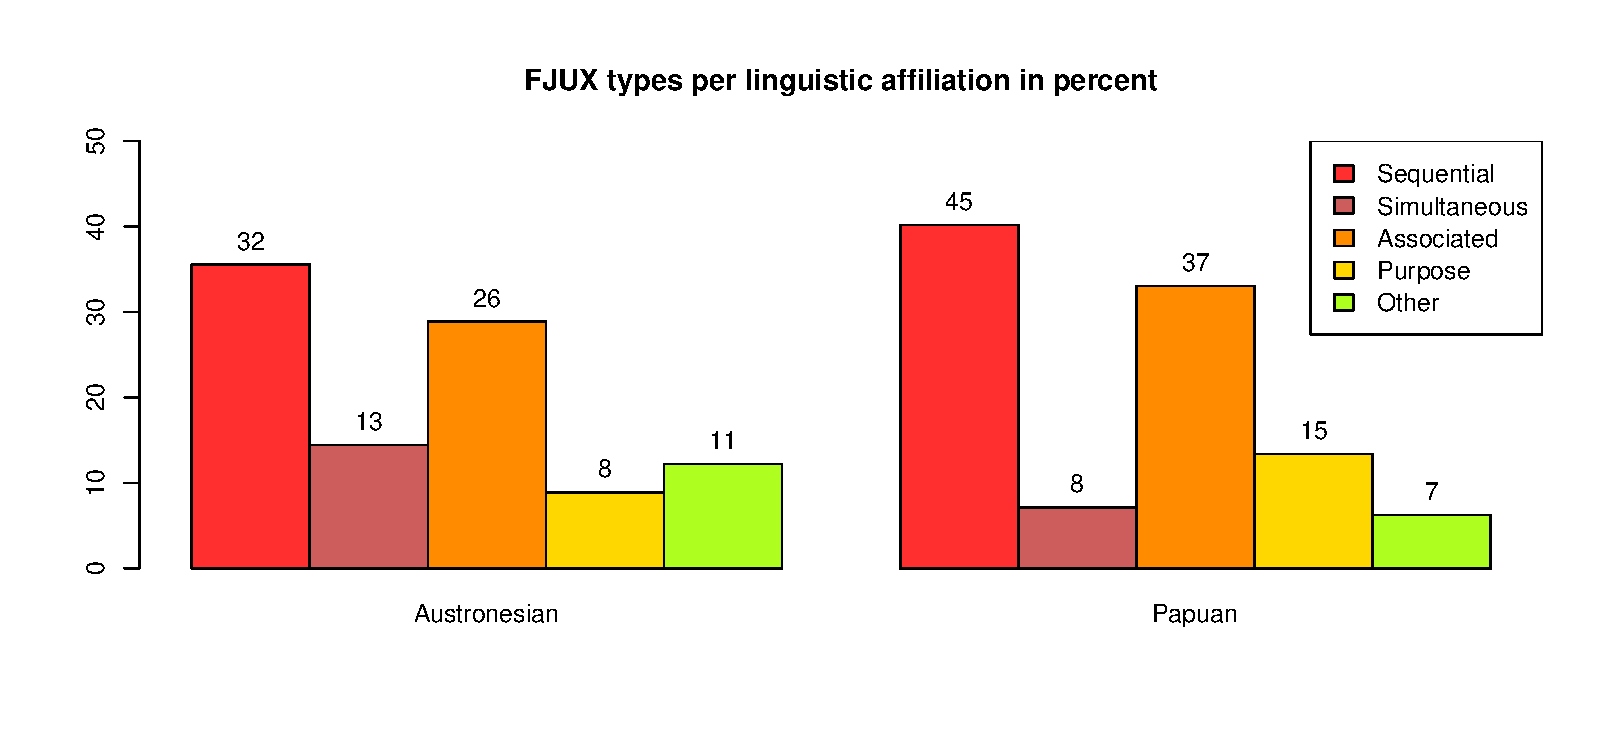
\includegraphics[width=\columnwidth]{figures/FJUX_family.eps}
\caption[FJUX types per linguistic affiliation in percent]{FJUX types per linguistic affiliation in percent. Numbers on top of the bars refer to the number of observations in the sample.}\label{fig:fjux-family}
\end{figure}
\begin{figure}
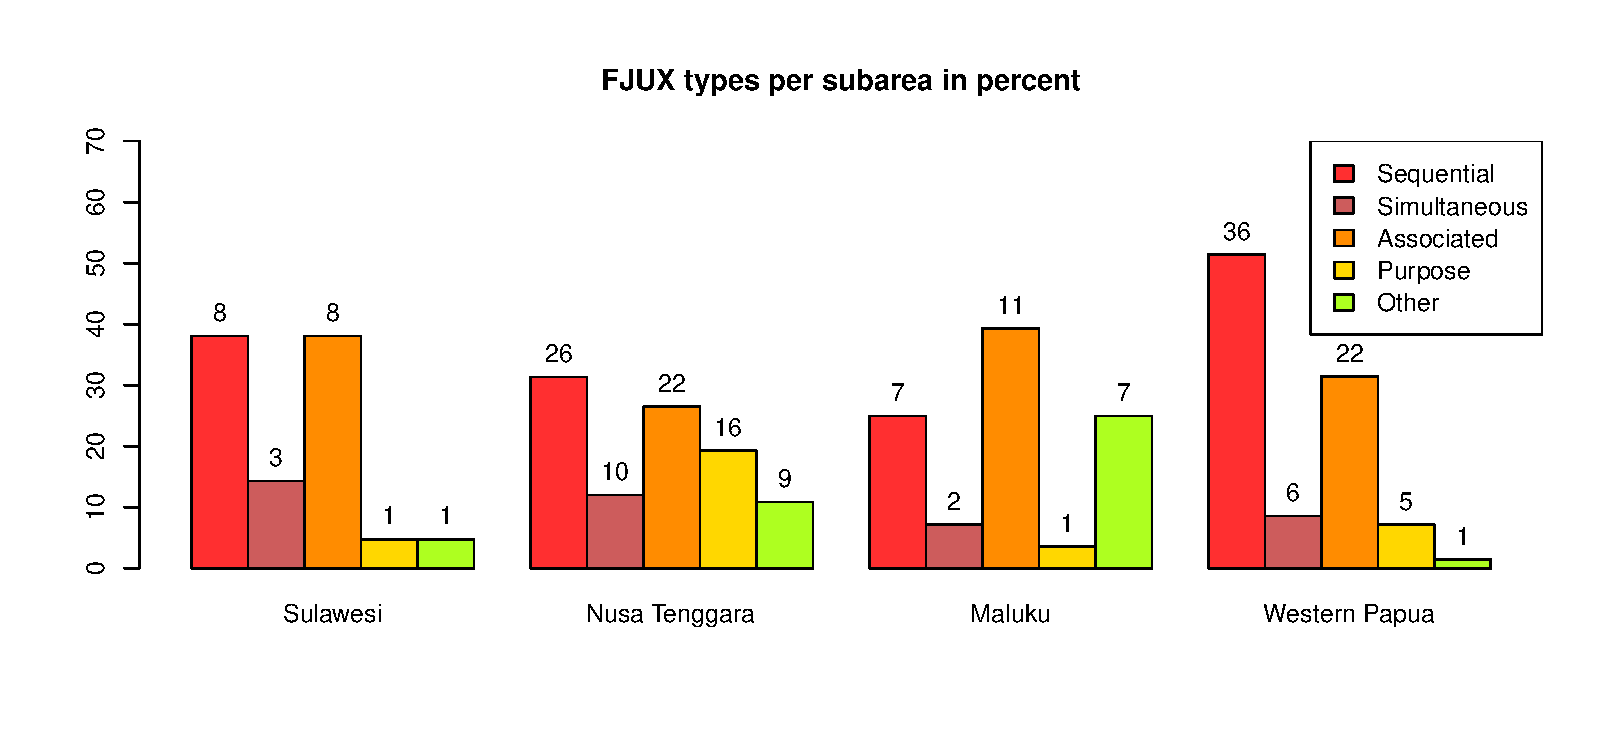
\includegraphics[width=\columnwidth]{figures/FJUX_group.eps}
\caption[FJUX types per subarea in percent]{FJUX types per subarea in percent. Numbers on top of the bars refer to the number of observations in the sample.}\label{fig:fjux-group}
\end{figure}

%The distribution of FJUX constructions per language is shown in \tabref{table:FJUX_language}. 
It is apparent that the numbers are unevenly distributed across the languages. Some languages that are otherwise subject to a high use of different MVC types, such as Abui or Makalero, only show weak traces of FJUX use. Other languages with only moderate use of MVC types, such as Mpur or Waima'a, show, for some categories, rather high numbers of occurrence. This appears to reflect different traits, both linguistic and methodological. If we compare the two corpus languages Waima'a and Wooi with over 170 data points each, we observe that the number of attested FJUX constructions is rather high in Waima'a, and quite low in Wooi. We can conclude that an increase in the number of data points appears to have an effect on FJUX retrieval only in Waima'a, but not in Wooi. This seems to indicate that not all EI languages make regular use of FJUX constructions. Another effect that shines through the distribution of FJUX cases is the focus of the researcher, and the extent of his or her grammatical description. So, for instance, while most Teiwa examples of sequential MVCs were found in Klamer's chapter on serial verb constructions \citep{klamer2010grammar}, the Mpur examples were (all but one) retrieved from an appended text in \citet{ode2002sketch}. Given that such additional data sources were not available for all languages, chances are high that some languages that appear to make only little use of FJUX constructions are in fact undersampled.

%\begin{table}
%\begin{footnotesize}
%\begin{tabular}{lrrrrr}
%  \midrule
% & {sequential} & {simultaneous} & {associated} & {purpose} & {other} \\ 
%  \midrule
%  Muna &   1 &   1 &   6 &   1 &   1 \\ 
%  Pendau &   0 &   1 &   0 &   0 &   0 \\ 
%  Tajio &   2 &   1 &   1 &   0 &   0 \\ 
%  Tolaki &   2 &   0 &   0 &   0 &   0 \\ 
%  TukangBesi &   3 &   0 &   1 &   0 &   0 \\ %\midrule
%  Abui &   1 &   0 &   1 &   2 &   2 \\ 
%  Alorese &   0 &   0 &   0 &   2 &   1 \\ 
%  Bunaq &   0 &   0 &   0 &   3 &   0 \\ 
%  Kaera &   0 &   0 &   0 &   1 &   0 \\ 
%  Kambera &   1 &   1 &   1 &   0 &   0 \\ 
%  Klon &   0 &   0 &   5 &   2 &   0 \\ 
%  Makalero &   1 &   0 &   1 &   0 &   0 \\ 
%  Teiwa &  13 &   2 &   2 &   3 &   1 \\ 
%  Tetun &   3 &   0 &   0 &   0 &   0 \\ 
%  Waima'a &   7 &   7 &  12 &   2 &   5 \\ 
%  Western Pantar &   0 &   0 &   0 &   1 &   0 %\\  \midrule
%  Buru &   0 &   0 &   1 &   0 &   3 \\ 
%  Selaru &   1 &   0 &   1 &   0 &   1 \\ 
%  Taba &   2 &   0 &   0 &   0 &   0 \\ 
%  Tidore &   2 &   0 &   8 &   0 &   3 \\ 
%  Tobelo &   2 &   2 &   1 &   1 &   0 \\ \midrule
%  Abun &   2 &   0 &   2 &   0 &   0 \\ 
%  Biak &   1 &   0 &   0 &   1 &   0 \\ 
%  Dusner &   0 &   0 &   3 &   2 &   0 \\ 
%  Hatam &   2 &   0 &   0 &   0 &   0 \\ 
%  Inanwatan &   3 &   0 &   4 &   0 &   0 \\ 
%  Maybrat &   4 &   2 &   3 &   0 &   0 \\ 
%  Mor &   4 &   2 &   0 &   0 &   0 \\ 
%  Moskona &   2 &   0 &   4 &   0 &   0 \\ 
%  Mpur &  13 &   2 &   1 &   0 &   1 \\ 
%  Sougb &   0 &   0 &   5 &   2 &   0 \\ 
%  Wooi &   5 &   0 &   0 &   0 &   0 \\ 
%   \midrule
%\end{tabular}
%\end{footnotesize}
%\caption[Distribution of FJUX types per language]{Distribution of FJUX types per language.}
%\label{table:FJUX_language}
%\end{table}

\tabref{table:FJUX_formal} below presents the morphosyntactic properties of FJUX constructions. If FJUX constructions are formed at the discourse level, and link independent CLEs together, one might expect a higher amount of variation in formal coding than found with the other constructional families. This appears to be the case, although the prototypical formal setup of MVCs in EI is still visible: most FJUX constructions show shared subjects (``S"), both verbs are inflected (``B"), and the verbals stand next to each other without intervening constituents (``C"). Some factorial values are unattested, again matching the prediction. For instance, both participant accumulation (``A") and event-to-argument reanalysis (``E") are hardly or not at all attested. As such referential expressions would point to a close semantic relationship between the CLEs, its absence is predictable. The same goes for headedness patterns denoting a more intricate interplay of the verbal constituents. Both partial head-marking (``1" and ``2") and shared marking (``S") are clearly dispreferred with FJUX constructions, as are within-word construals (``W"). The opposite is true for indicators of lower constructional cohesiveness. No referential interaction (``X") occurs frequently, and the contiguity values exceed the ``C" pattern in many cases, i.e., one or more constituents are found to intervene between the verbs.

\begin{table}
\centering
\begin{tabular}{rrrrrrr}
  \lsptoprule
Referentiality & S & SO & D & E & X \\ 
  \midrule
  sequential &  52 &   4 &   8 &   1 &  12 \\ 
  simultaneous &  18 &   0 &   0 &   0 &   3 \\ 
  associated &  42 &   3 &   6 &   1 &  11 \\ 
  purpose &  10 &   0 &  11 &   0 &   2 \\ 
  other &  17 &   0 &   0 &   0 &   1 \\ 
   \midrule
 \\
  \midrule
Headedness & B & 1 & 2 & S & N \\ 
  \midrule
  sequential &  44 &   1 &   2 &   0 &   3 \\ 
  simultaneous &  12 &   0 &   0 &   0 &   0 \\ 
  associated &  30 &   2 &   1 &   1 &   5 \\ 
  purpose &   7 &   0 &   0 &   0 &   0 \\ 
  other &   3 &   0 &   0 &   0 &   3 \\ 
   \midrule
 \\
  \midrule
Contiguity & W & C & 1 & 2 & 3 & 4 \\ 
  \midrule
  sequential &   0 &  35 &  31 &  10 &   1 &   0 \\ 
  simultaneous &   0 &  17 &   2 &   2 &   0 &   0 \\ 
  associated &   0 &  33 &  20 &   7 &   2 &   1 \\ 
  purpose &   0 &   8 &  11 &   3 &   1 &   0 \\ 
  other &   2 &  15 &   0 &   1 &   0 &   0 \\ 
   \lspbottomrule
\end{tabular}
\caption[Morphosyntactic properties of FJUX constructions]{Morphosyntactic properties of FJUX constructions in EI. Table components from top to bottom refer to referentiality (see §\ref{sec:argumentstructure}), headedness (see §\ref{sec:headedness}), and contiguity (see §\ref{sec:contiguity}), respectively. Referentiality values: S = Co-functional (``same subject"), SO = Transitive co-functional (``same subject and object"), D = Switch-function (``Different subject"), A = Participant accumulation, E = Event-to-argument (``Ambient"), X = no interaction, no arguments shared. Headedness values: B = Both verbs marked, 1 = First verb marked, 2 = Second/final verb marked, S = Shared affix set, N = None of the verbs marked. Contiguity values: W = Within word, C = Contiguous verbs 1 = One non-verbal constituent intervening, 2 = Two non-verbal constituents intervening, 3 = Three non-verbal constituents intervening, 4 = Four non-verbal constituents intervening.}
\label{table:FJUX_formal}
\end{table}

As in the previous parts of this chapter, the next sections explore the FJUX types in some more detail, and provide examples from the different subareas.

\subsection{Sequential}

Sequential MVCs mostly correlate dynamic eventualities, and almost no stative verbs are employed. The constructional meaning is such that both events occur in temporal sequence without, however, an explicit account of how the events are related. Despite the low number of cases, it can be seen from \tabref{table:sequential} that sequential MVCs can be found in most of the EI languages.

\begin{table}
\begin{tabular}{ll}
\lsptoprule
Feature&Value\tabularnewline
\midrule
Template& V1 \textsc{dynamic verb} -- V2 \textsc{dynamic verb}\tabularnewline
No. of attested instances& 77/2146 \tabularnewline
No. of attested languages& 23/32 \tabularnewline
Distribution across areas& \textsc{sul} (4/5), \textsc{nus} (6/11), \textsc{mal} (4/5), \textsc{pap} (9/11) \tabularnewline
Distribution across families& \textsc{pap} (11), \textsc{aus} (12) \tabularnewline
\lspbottomrule
\end{tabular}
\caption[Template and basic distribution of sequential MVCs]{Template and basic distribution of sequential MVCs in the EI sample.}
\label{table:sequential}
\end{table}

The following examples demonstrate that sequential MVCs can adapt to many different contexts and communicative situations. Example (\ref{Tukang_49}) from Tukang Besi depicts a classical combination of two dynamnic events. The second event begins just when the first event happens to end. There is no specific relation between the gossiping and the continuing, such as causal or consecutive relations. Notice also that there is no referential identity in the narrow sense. 

\ea \label{Tukang_49}
\langinfo{Tukang Besi}{Austronesian, WMP}{\citealt[503]{donohue1999}}\\
\gll po'oli ko-tula-tula ku-torusu-mo ku(a) koranga \\
finish 1\textsc{pa}.\textsc{rls}-\textsc{rdp}-tale 1\textsc{sg}-continue-\textsc{prfv} \textsc{all} garden \\
\glft `After we had gossiped, I continued on to the garden.'\\ 
\z

Another group of sequential MVCs denotes action sequences in which the actor remains constant. The next two examples in (\ref{Tetun_13}) and (\ref{Tidore_87}) from Tetun and Tidore, respectively, illustrate such use. In example (\ref{Tetun_13}), we can see a sequence of seven verbs. \citet{vanklinken1999grammar} tentatively placed clausal boundaries between \textit{manas} and \textit{hodi}, and between \textit{mai} and \textit{sia}, but from the lack of prosodic and syntactic boundary clues one could also argue for a free juxtaposition of several smaller MVCs that are aligned here because they all happen in what is perceived as one discourse sequence. It is remarkable that the verbal building blocks fall into MVC types that are immediately recognisable: \textit{bá te'in} form a motion-to-action construction, \textit{nono wé manas} constitute a resultative construction, and \textit{hodi mai} is a transport complex. Two linkings, however, do not fit into any of the constructions types discussed previously in this chapter. First, there is no construction that would comprise a combination of cooking and heating. As both verbs are at least in this context quasi synonymous they can be regarded as a lexicalised combination, created by stylistic conventions rather than by communicative needs (recall the synonymous verbs from §\ref{sec:other}). And second, bringing and drinking is special due to the change in referential expression. It is not the actor bringing the hot water that drinks it afterwards. Rather the construction looks like a purpose construction (I will come back to this type in section §\ref{sec:purpose}). 

\ea \label{Tetun_13}
\langinfo{Tetun Fehan}{Austronesian}{\citealt[253]{vanklinken1999grammar}}\\
\gll bá te'in nono wé manas hodi mai sia r-emu \\
go cook heat(.liquid) water hot bring come 3\textsc{pl} 3\textsc{pl}-drink \\
\glft `[Then] (I) went and boiled water and brought (it and) they drank [, and they ate.]'\\ 
\z

The verb string in example (\ref{Tidore_87}) denotes a procedure involving three actions (all having a different object). Each step leads to the next one until the body of the participant is smeared with fish blood. Such procedures are often associated with manual action, and there are several cases of FJUX attested for such procedurals in the sample.

\ea \label{Tidore_87}
\langinfo{Tidore}{Papuan, NH}{\citealt[368]{vanstaden2000tidore}}\\
\gll Ah, ona yau wako isa=ge, ona suka nyao ngge oro ena ma-au se-baca una i-rehe ena=ge \\
ah 3\textsc{pl} to.fish return landwards=there 3\textsc{pl} break fish 3\textsc{nhum}.there take 3\textsc{nhum} 3\textsc{nhum}.\textsc{pos}-blood \textsc{caus}-\textsc{nm}.rub 3\textsc{sg}.\textsc{m} 3\textsc{sg}.\textsc{m}.\textsc{pos}-body 3\textsc{nhum}=there \\
\glft ‘So when they returned from fishing they cut up a fish and took its blood and rubbed his body.’\\ 
\z

The last example is from Abun. As in example (\ref{Tetun_13}) from Tetun, it appears to juxtapose two MVCs, a motion-to-action construction and a transport complex, together. Unfortunately, Berry and Berry's grammar of Abun does not provide appended texts, and it cannot be ascertained at this point whether FJUX construals are a regular means of composing MVCs in Abun. What is remarkable with such conjoined MVCs is that they form templates just as the ones Pawley describes for Kalam.

\ea \label{Abun_4}
\langinfo{Abun}{Papuan, isolate}{\citealt[52]{berry1999}}\\
\gll ye-suk-mise ma nai gwat an mu ket \\
\textsc{pers}-\textsc{nm}-evil come capture carry 3\textsc{sg} go west \\
\glft `The police came and caught him and took him westward.'\\ 
\z

\subsection{Simultaneous} \label{sec:simultaneous}

Simultaneous \textsc{MVC}s are vey infrequent in the EI sample, with only 21 examples from ten languages. \tabref{table:simultaneous} provides the numbers. Most simultaneous instances denote a motion event, together with another action that is carried out by the moving participant. There are no stative verbs found in simultaneous MVCs.

\begin{table}
\begin{tabular}{ll}
\lsptoprule
Feature&Value\tabularnewline
\midrule
Template& V1 \textsc{dynamic verb} -- V2 \textsc{dynamic verb}\tabularnewline
No. of attested instances& 21/2146 \tabularnewline
No. of attested languages& 10/32 \tabularnewline
Distribution across areas& \textsc{sul} (3/5), \textsc{nus} (3/11), \textsc{mal} (1/5), \textsc{pap} (3/11) \tabularnewline
Distribution across families& \textsc{pap} (4), \textsc{aus} (6) \tabularnewline
\lspbottomrule
\end{tabular}
\caption[Template and basic distribution of simultaneous MVCs]{Template and basic distribution of simultaneous MVCs in the EI sample.}
\label{table:simultaneous}
\end{table}

Here are two examples of simultaneous MVCs. Example (\ref{Pendau_4}) from Pendau illustrates the combination of a manner of motion verb with a state change verb. As the flying proceeds, the shapes of the referents become smaller against the sky. Note that the aspectual clitic \textit{=mo} attaches to the last verb in the series, and the scope of the completive is over the whole simultaneous construction. Similar scope behaviour can also be observed in other EI languages. Take the example from Teiwa in (\ref{Teiwa_37}) in which a progressive marker is placed in construction-final position. Here, as well, it seems that the scope of \textit{pati} is over the whole construction. 

\ea \label{Pendau_4}
\langinfo{Pendau}{Austronesian, WMP}{\citealt[335]{Quick2007}}\\
\glll bai uo nolumeap nkaasimo, jimo no'umene' \\
bai 'uo N-po-[um]-leap no-kaasi=mo jimo no-'u-mene' \\
like yonder \textsc{rls}-\textsc{sf}-\textsc{tel}-fly \textsc{st}.\textsc{rls}-shrink=\textsc{compl} 3\textsc{pl}.\textsc{abs} \textsc{ug}.\textsc{rls}-\textsc{sf}-go.up \\
\glft `So as they flew up they shrunk (in apparent size), and they went up.'\\ 
\z

\ea \label{Teiwa_37}
\langinfo{Teiwa}{Papuan, TAP}{\citealt[312]{klamer2010grammar}}\\
\gll bai qavif non saxa' rau, kamau, a-tan pin-an soxai pati \\
pig goat \textsc{pl} chicken civet.cat cat \textsc{top} 3\textsc{sg}-stand hold-\textsc{rls} dance \textsc{prog} \\
\glft `[the] pigs, goats, chicken, civet cats, cats, who were holding hands while dancing.'\\ 
\z

Teiwa, as well as other EI languages, also has formal means to conjoin two eventualities. In Teiwa, there is a junctor \textit{si} that correlates two clauses the eventualities of which happen at the same time. While cases like example (\ref{Teiwa_37}) still appear to form a tight construal, and share their subject referents, simultaneous structures marked with \textit{si} appear to combine larger units. Consider the following example. There is a switch in reference between both events. The subject of V$_1$ becomes the goal of the climbing. Such simultaneous markers are also attested in other EI languages. If they constitute clause linking devices, then the simultaneous MVCs illustrated above still produce more compressed biclausal structures, or may even turn out to form a single clause, as the operator behaviour seems to suggest in some cases.

\ea 
\langinfo{Teiwa}{Papuan, TAP}{\citealt[257]{klamer2010grammar}}\\
\gll ti'-in, iqa'an ga'an u a un tii'-in si ilan mir \\
sleep-\textsc{rls} dark 3\textsc{sg} \textsc{dist} 3\textsc{sg} \textsc{cont} sleep-\textsc{rls} \textsc{sim} grow.up ascend \\
\glft `Sleeping...that night he was sleeping while [something] came up [to him].'\\ 
\z

\subsection{Associated}

In associated MVCs the temporal relation between the verbs seems less prominent than in the sequential or simultaneous construction. What is foregrounded instead is a general notion of both eventualities being associated with each other. This association is in most cases reminiscent of semantic relations otherwise found in clause subordination, such as conditional, adversative, or conclusive semantics. In some cases, but not in all, a junctor may be placed between the verbs without any apparent change in meaning. With only 20 attested cases, associated MVCs lack sufficient data for a more detailed analysis, and I doubt that, with more data at hand, this will turn out to be a coherent construction throughout EI. \tabref{table:associated} illustrates the basic numbers.

\begin{table}
\begin{tabular}{ll}
\lsptoprule
Feature&Value\tabularnewline
\midrule
Template& V1 \textsc{verb} -- V2 \textsc{verb}\tabularnewline
No. of attested instances& 63/2146 \tabularnewline
No. of attested languages& 20/32 \tabularnewline
Distribution across areas& \textsc{sul} (3/5), \textsc{nus} (6/11), \textsc{mal} (4/5), \textsc{pap} (7/11) \tabularnewline
Distribution across families& \textsc{pap} (11), \textsc{aus} (12) \tabularnewline
\lspbottomrule
\end{tabular}
\caption[Template and basic distribution of associated MVCs]{Template and basic distribution of associated MVCs in the EI sample.}
\label{table:associated}
\end{table}

Consider the following examples. In example (\ref{Muna_2}) from Muna we can see a MVC that looks just like a conditional clause. \citet{vandenberg1989} remarks that one may add the conditional marker \textit{ane} here without making any change to the meaning. While the singing appears to refer to an individuable spatiotemporal event, the voice being beautiful can be regarded as an individual-level predicate that holds true not only at the time of the singing, but constitutes a permanent property of the participant. Therefore, such construals seem to be different from simultaneous MVCs where two actions are correlated and performed by one single actor. The next example in (\ref{Teiwa_74}) is from Teiwa and illustrates adversative semantics. This example  demonstrates a case in which no referential interaction takes place (no argument sharing, ``X" pattern). Note also that the second clause is negated with \textit{maan}, while the first clause is not. This is a strong clue that we are dealing here with two independent clauses.

\ea \label{Muna_2}
\langinfo{Muna}{Austronesian, WMP}{\citealt[235]{vandenberg1989}}\\
\gll nao-kesa sepaliha dua suara-no (ane) nae-lagu \\
3\textsc{sg}.\textsc{irr}-beautiful very also voice-his (if) 3\textsc{sg}.\textsc{irr}-sing \\
\glft `His voice will also be very beautiful when he sings.'\\ 
\z

\ea \label{Teiwa_74}
\langinfo{Teiwa}{Papuan, TAP}{\citealt[355]{klamer2010grammar}}\\
\gll suk-an maan kri u pak-an pak-an suk-an maan \\
exit.come.down-\textsc{rls} \textsc{neg} Mr \textsc{dist} call-\textsc{rls} call-\textsc{rls} exit.come.down-\textsc{rls} \textsc{neg} \\
\glft `They didn't come out, that grandfather called and called [but] no-one came out...'\\ 
\z

The next example from Tobelo shows two conjoined statives. Just like \textit{kesa} `be beautiful' in example (\ref{Muna_2}) from Muna, \textit{bole} `be tired' and \textit{timono} `old' are, in my view, understood as individual-level predicates, denoting permanent properties of the participant. Although one may claim that both states hold true at event time, they hardly constitute simultaneous events in the sense discussed in §\ref{sec:simultaneous}. The last example in (\ref{Sougb_36}) from Sougb shows two action verbs, \textit{(o)uhw} `trade' and \textit{ebe-piara} `do-look.after', that occur in temporal sequence, but differ from typical sequential constructions in that the second verb projects an event that extends over years instead of denoting a concrete (manual) action within a limited time span. A second property that is not found in prototypical sequential MVCs is the function switch from first person object to first person subject. The first person participant here acts like a pivotal argument, leading to what seems to be an overlap of two clauses. Indeed, such construals bear a resemblance to those constructions in West African languages that \citet{ameka2005multiverb} described as overlapping constructions.

\ea 
\langinfo{Tobelo}{Papuan, NH}{\citealt[68]{holton2003tobelo}}\\
\gll i-hi-bole-oka i-hi-timono-oka ho to-oiki-oka-ua \\
3-1-tired-\textsc{prfv} 3-1-old-\textsc{prfv} thus 1-go-\textsc{prfv}-\textsc{neg} \\
\glft `I was old and tired, so I didn't want to go again.'\\ 
\z

\ea \label{Sougb_36}
\langinfo{Sougb}{Papuan, EBH}{\citealt[269]{reesink2002grammar}}\\
\gll dan d-ouma, gida hom, ka lan la-(o)uhw dou dan d-ebe-piara \\
I 1\textsc{sg}-buy female one then they.\textsc{du} 2\textsc{du}-trade to I 1\textsc{sg}-do-look.after \\
\glft `I would buy one girl and they'd trade her to me and I would look after her.'\\ 
\z

In the next section, I turn to purpose MVCs that also appear to be construed much like overlapping constructions in West African languages.

\subsection{Purpose} \label{sec:purpose}

Purpose MVCs combine two action predicates, of which the second one denotes the outcome or purpose of the first action. The actor of the first predicate is typically not maintained in the second predicate. The most frequent verb in V$_1$ is a verb of giving or putting. An actor transfers some object to another (group of) participant(s) in order for them to perform some other action. Given that the number of attested constructions is quite low in the sample, the number of languages with attested cases is rather high (n=13). We can see from \tabref{table:purpose} that the use of the purpose construction is predominantly found in Nusa Tenggara languages.

\begin{table}
\begin{tabular}{ll}
\lsptoprule
Feature&Value\tabularnewline
\midrule
Template& V1 \textsc{dynamic verb} -- V2 \textsc{dynamic verb}\tabularnewline
No. of attested instances& 23/2146 \tabularnewline
No. of attested languages& 13/32 \tabularnewline
Distribution across areas& \textsc{sul} (1/5), \textsc{nus} (8/11), \textsc{mal} (1/5), \textsc{pap} (3/11) \tabularnewline
Distribution across families& \textsc{pap} (8), \textsc{aus} (5) \tabularnewline
\lspbottomrule
\end{tabular}
\caption[Template and basic distribution of purpose MVCs]{Template and basic distribution of purpose MVCs in the EI sample.}
\label{table:purpose}
\end{table}

The following examples present typical cases from different subareas. In example (\ref{Bunaq_4}) from Bunaq, a \textsc{give} verb is combined with a verb of food consumption. This is indeed the most widespread combination (mostly with \textsc{eat} verbs). Schapper analysed this construction type as causative SVCs, ``expressing purposive causation in transfer events" \citep[446]{schapper2009bunaq}. Arguably, there is indeed some sense of causation involved between the transfer and the consequent action in that it is the transfer that \emph{enables} the second action to be carried out. Such construals of causation differ, however, from direct causation, as construed by cause-result, causative or resultative constructions in the EI area. While in those constructions we may say that the initial causing event directly triggers the resultant event (for instance, because some force is applied to a patient participant), in purpose MVCs the second action may or may not be carried out. It seems that the purposive reading leaves the actual performance of the second event unexpressed. So, for instance, in example (\ref{Bunaq_4}) we do in fact not really know whether the drinking event will take place or not. It is only that the transfer enables the third person participant to carry out the drinking. 

\ea \label{Bunaq_4}
\langinfo{Bunaq}{Papuan, TAP}{\citealt[446]{schapper2009bunaq}}\\
\gll neto baqi g-ege il a \\
1\textsc{sg} \textsc{nprx}.\textsc{an} 3\textsc{an}-give water drink \\
\glft ‘I gave him water to drink.’\\ 
\z

This non-realis interpretation of the second action becomes visible when negation is applied to the construction, as we can see in example (\ref{Bunaq_4b}) below. While it is fine for the negator to have scope over the whole construction, it may not be place before the second verb. This suggests that the drinking may not be negated because it has in fact not yet taken place. 

\ea \label{Bunaq_4b}
\langinfo{Bunaq}{Papuan, TAP}{\citealt[446]{schapper2009bunaq}}\\
\ea
\gll neto baqi g-ege il a niq \\
1\textsc{sg} \textsc{nprx}.\textsc{an} 3\textsc{an}-give water drink \textsc{neg} \\
\glft ‘I did not give him water to drink.’ \\ 
\ex
\gll *neto baqi g-ege niq il a \\ 
1\textsc{sg} \textsc{nprx}.\textsc{an} 3\textsc{an}-give \textsc{neg} water drink \\
\z
\z

Example (\ref{Alorese_17}) from Alorese suggests a similar MVC. The transfer of pictures is intended to let another participant look at them. Notice that the first person referent is expressed here twice by a free pronoun. Expressing one participant twice would be clearly dispreferred in most MVC types with a closer packing of LLEs, and this can be interpreted as another clue for rather loose bonds between the two predicates here. Example (\ref{Tobelo_16}) from Tobelo shows yet another combination of verbs. In this example, the actors stay the same across both predicates, but the translation still indicates a purposive interpretation. Finally, the Dusner example in (\ref{Dusner_4}) illustrates another purposive combination with an \textsc{eat} verb in final position. Here as well, the actor is the same in both predicates.

\ea \label{Alorese_17}
\langinfo{Alorese}{Austronesian, CMP}{\citealt[72]{klamer2011alorese}}\\
\gll mi neng go foto go seru \\
2\textsc{pl} give 1\textsc{sg} photograph 1\textsc{sg} see \\
\glft `You show me (some) pictures.' (Lit. You give me pictures I see) \\ 
\z

\ea \label{Tobelo_16}
\langinfo{Tobelo}{Papuan, NH}{\citealt[61]{holton2003tobelo}}\\
\gll yo-karajanga o-lapangan yo-diai \\
3\textsc{pl}-work \textsc{nm}-field 3\textsc{pl}-make \\
\glft `We [sic] worked to make an airfield.' \\ 
\z

\ea \label{Dusner_4}
\langinfo{Dusner}{Austronesian, SHWNG}{\citealt[19]{dalrymple2012}}\\
\glll yave o verano yan \\
ya-ve o Ø-ve-ran=o y-an \\
1\textsc{sg}-say \textsc{exclam} 1\textsc{sg}-\textsc{vblz}-sago=\textsc{fill} 1\textsc{sg}-eat \\
\glft `I said: Oh, I can make papeda (sago porridge) to eat.'\\ 
\z

\subsection{Other}

The final group of examples from free juxtaposition constructions comprise two smallish sets of MVCs. First, there are two cases of delimitative MVCs (do x \textit{until} y happens), one from Mpur and another one from Muna. I have already discussed this construction at the beginning of §\ref{sec:fjux}, and have nothing to add here. Second, there is a small set of verb collocations that appear to be, to a certain extent, lexicalised, and thus may occur together in fixed chunks. I will not have much to say about these groups as there is so little data available. Neither is it possible to examine in detail whether these collocations really do behave as fixed expressions, so that some of these cases might instead simply turn out to be ``the odd ones out".

As lexicalised verb strings may even exhibit word-like properties, their placement within free juxtaposition constructions is clearly only preliminary. Although lexicalised construals would arguably be construed rather tightly, I assume that they might have originated in more loose collocations. \tabref{table:other_fjux} illustrates the distribution of this heterogeneous group. Lexicalised MVCs of different kinds seem to be more in use in Nusa Tenggara and Maluku. 

\begin{table}
\begin{tabular}{ll}
\lsptoprule
Feature&Value\tabularnewline
\midrule
Template& V1 \textsc{dynamic verb} -- V2 \textsc{dynamic verb}\tabularnewline
No. of attested instances& 18/2146 \tabularnewline
No. of attested languages& 9/32 \tabularnewline
Distribution across areas& \textsc{sul} (1/5), \textsc{nus} (4/11), \textsc{mal} (3/5), \textsc{pap} (1/11) \tabularnewline
Distribution across families& \textsc{pap} (4), \textsc{aus} (5) \tabularnewline
\lspbottomrule
\end{tabular}
\caption[Template and basic distribution of other FJUX MVCs]{Template and basic distribution of other FJUX MVCs in the EI sample.}
\label{table:other_fjux}
\end{table}

We have already seen one type of lexicalised MVC in the component-relating family, namely synonymous MVCs (see §\ref{sec:other}). I argued there that synonymous CRELs bear a resemblance to other component-relating constructions as the verbs obviously share at least some part of their semantic structure. Some authors have extended the notion of synonymous SVCs to cases in which two verbs with related semantics (from the ``same semantic field") are combined. Example (\ref{Abui_34}) from Abui shows two such MVCs. The first pair of verbs with somewhat ``related semantics" is \textit{t} `lie' and \textit{wel} `pour', at least understood in a non-literal sense as pertaining to daily processes in the upbringing of a child. Another pair is claimed to consist of \textit{fok-d} `big-hold' and \textit{fin-r} `eldest-reach', both relating to growing up in a wider sense. Kratochvíl placed these constructions with the group of synonymous SVCs, and remarked that ``[t]hese parallel expressions seem to be lexicalized or at least highly conventionalized" (2007: 357). The difference to synonymous MVCs \textit{sensu stricto}, however, is that the verbs only share very unspecific meaning components, if any at all.

\ea \label{Abui_34}
\langinfo{Abui}{Papuan, TAP}{\citealt[357]{kratochvil2007grammar}}\\
\gll na a-t a-wel-i ba he-fokda he-fin-r-i \\
1\textsc{sg} 2\textsc{sg}.\textsc{pat}-lie 2\textsc{sg}.\textsc{pat}-pour-\textsc{prfv} \textsc{lnk} 3\textsc{loc}-grow.up 3\textsc{loc}-eldest-reach-\textsc{prfv} \\
\glft ‘I took care of you till you grew up.’ (lit: ‘I fed and washed you until you grew up and
became adult’)\\
\z

Another example of lexicalised MVCs is the following combination of a \textsc{see} verb and a \textsc{find} verb from Waima'a. The examples are from two pear story narrations, each narrated by a different speaker. Both speakers use exactly the same construction at the point where the boy is handed back his hat. Note that both verbs are placed next to each other, and all expressed arguments are found either before or after the verb complex.

\ea 
\langinfo{Waima'a}{Austronesian, CMP}{pear\_Bendita 039}\\
\gll ne: buni hita hile lo ne zapeu nini \\
\textsc{foc} see find again \textsc{asp} 3\textsc{sg} hat \textsc{poss} \\
\glft `...and found his hat.'\\ 
\z

\ea 
\langinfo{Waima'a}{Austronesian, CMP}{pear\_Santina 171}\\
\glll ne bun hita sapeo anse \\
ne buni hita sabeo ana-see \\
\glc 3\textsc{sg} see find hat \textsc{clf}-one \\
\glft `He finds a hat...' \\ 
\z

In the light of what I have discussed in this chapter and the previous one, free juxtaposition constructions are ephemeral constructions that can be perceived as \textit{ad hoc} formations on the discourse-level rather than as fixed constructions with rigid constructional blueprints, such as, say, motion complex MVCs with their invariant order ot motion verb classes. Rather, any combination of verbs seems licit as long as more general rules of semantic clause linking are adhered to. In this view, lexicalised, or at least condensed verb structures without a host class slot, such as we have seen in the Waima'a examples above, do not seem to fit into the FJUX category, and may instead constitute a category of their own.

\section{Summary}

This chapter explored the sample with regard to constructional types and their distribution across Eastern Indonesia. By combining the morphosyntactic findings from Chapter \ref{ch:gram} with the semantic theory of MVC formation on different conceptual levels developed in Chapter \ref{ch:sem}, I proposed four families of MVCs used throughout the region. Each constructional family is based upon one underlying technique of MVC formation. While both component-relating constructions and modifying constructions constitute single-stage MVCs with only one individuable event stage based on a single (combined) event argument, stage-relating constructions and free juxtaposition constructions correlate two event expressions by forming a two-stage event schema. The event argument of each verb is in these types preserved, and each may in principle become the target of a grammatical operator. However, as we have seen, stage-relating constructions appear to be the result of a certain extent of grammaticalisation, at least in some of the EI languages, preventing the staged constituents to act like fully independent constituents. 

In §\ref{sec:criteria_mvcs} I presented a set of criteria that, when applied together, reveals differences between the four constructional families. The criteria were taken from four fields: argument structure, operator behaviour, constituency, and semantics. Four criteria set off FJUX constructions from the other three types. Obligatory argument interaction, identical TAM/person index values, and asymmetrical headedness are not found in FJUX, but in all other constructional families. Conjunction insertion, on the other hand, is only found with FJUX constructions. Five additional criteria distinguish the single-stage construction types CREL and MOD from the two-stage SREL and FJUX types. Both event-to-argument reanalysis and grammaticalisation of features in V$_2$ are associated with the former, but not with the latter. Partial temporal modification and sequential reading, on the other hand, are only indicative of the two-stage types, and not of the single-stage ones CREL and MOD. Partial negation appears to be licit in MOD and FJUX, but not in CREL and SREL. Finally, some criteria are unique to certain types. Obligatory constituent order is found with all types except MOD. MVC embedding seems possible with all types but CREL. And the notion of temporal immediacy holding between the verbs' event schemas is a feature of SREL constructions, but is not present in or not necessarily inferable from the other three types.

The distribution of MVCs is surprisingly even across linguistic affiliation and geographical subareas. Linguistic affiliation is, in all likelihood, not a major factor in predicting the occurrence of MVC types. The four subareas, Sulawesi, Nusa Tenggara, Maluku, and Western Papua, showed moderate differences in the use of MVC types. Modifying constructions were found to be most frequent in the former three subareas, while in Western Papua the use of component-relating constructions and stage-relating constructions was slightly more frequent than MOD constructions. Biclausal free juxtaposition constructions were in all four subareas only attested in small numbers. 

In the final chapter, I will attempt to review the findings from this book and draw some preliminary conclusions that arise from the data. The focus will be on interpreting the patterns of MVC usage further, and hinting at some observations that could not be included into the discussion of the previous chapters.
 
\chapter{Discussion}\label{ch:discussion}
\section{Introduction}

In the preceding chapters, I laid out an analysis of Eastern \ili{Indonesian} \textsc{multi-verb construction}s based on different perspectives. In Chapter \ref{ch:gram}, I investigated the morphosyntactic properties of MVCs that are accessible from published data sources. I focused on three factors: referential interaction between the participating verbs (argument sharing), inflection patterns (addressed in terms of headedness features), and placement options (contiguity) of the verbs. In Chapter \ref{ch:sem}, I then turned to a semantic perspective on MVCs, and proposed two semantic frameworks that may help categorise MVCs into types. By applying a lexical decomposition model and Davidsonian event arguments, I argued for a set of four techniques of verbal interaction underlying the wealth of MVCs in Eastern Indonesia: \textsc{merging}, \textsc{modification}, \textsc{staging} proper, and \textsc{free juxtaposition}. These four techniques were argued to each constitute a major family of MVCs. In Chapter \ref{ch:constructions}, I combined the findings from Chapter \ref{ch:gram} with a theory of MVC formation on different conceptual levels from Chapter \ref{ch:sem} in order to arrive at a classification of MVCs. The four basic constructional families were further elaborated, and furnished with examples and data on their occurrence and distribution in the area. \textsc{Component-relating construction}s were defined as those constructions that merge part of their sublexical components. Modifying constructions comprise a matrix verb that is complemented by a modifier verb adding specific semantic content. Unlike the merging scenario, modifying constructions do not consist of verbs that share sublexical features. Staging proper was claimed to underly \textsc{stage-relating construction}s that are composed of two independent event stages, each licensed by an event argument. Finally, a fourth family of constructions was identified that also aligns more than one \textsc{event stage}, albeit without signs of producing a coherent unit on different levels (that is, lacking a monoclausal reading, a coherent prosodic phrasing, and so on).

In the present chapter, I will pick up some of the loose threads from the preceding discussion, and work out at least to some extent how these findings can be interpreted and framed into a more coherent picture. As has become obvious throughout this book, a literature survey of published data is quite limited in various ways. Published primary data deny the analyst the possibility of thoroughly testing many of the claims raised in the serialisation literature. The nature of the current study prevented me from filling this lacuna by simply adding more data to my analysis; as a result, the findings gained from the EI sample remain to be explored further. Therefore, the discussion in the following sections should be understood as a collection of suggestive pieces of evidence hopefully stimulating further scrutiny. I will specifically focus on properties and patterns that can be addressed through my data annotation.

In §\ref{sec:distribution} I will review the EI sample with regard to the question of what the data can tell us about the distribution and diversity of MVCs across the area. I will try to show that the number of different constructions is only one possible indicator for the amount of MVC use per language. In order to account for the frequency of MVC use, a standardised sample would be needed for all languages. As this is beyond the scope of this book, I will take the number of attested instances as a preliminary measure of MVC diversity in a given language.

The following section §\ref{sec:hierarchy} then turns to another factor that may reveal the extent to which a given language utilises MVCs. I have already discussed in Chapter \ref{ch:theory} that some MVCs can be dissected into what I call \textsc{stacked MVCs}: more than one MVC nested into another. Taking this hypothesis seriously would mean rethinking the issue of hierarchies in MVCs. In this section, I will explore briefly what it means to postulate hidden hierarchies, and how the issue could be approached theoretically. I will then explore the EI sample by computing how many MVCs per language are in fact complex, in the sense that they contain another MVC at a lower level.

In §\ref{sec:profile_use}, I will compare the results obtained from the previous two sections, and propose a broad typology of MVC use across EI. I will distinguish between four different usage profiles. Mapping these profiles on the EI languages will show that languages from all four subareas vary considerably in the extent to which MVCs pervade their grammatical system. Despite this variation, two major core areas of MVC use can be identified.

§\ref{sec:discourse} shifts the perspective back to an issue that I raised before in the discussion of prosodic properties of MVCs (chapter \ref{ch:theory}). It is far from clear, and actually quite improbable, that the syntactic boundaries of MVCs always match with prosodic boundaries. The criterion of coherent, or even ``monoclausal", intonation units for MVCs is thus hardly sustainable, and would probably not be borne out by a more comprehensive investigation into natural speech data. Although it is beyond the scope of this book to carry out such an analysis, §\ref{sec:discourse} will nonetheless gather evidence from some of the languages in order to point out some remarkable pieces of evidence. Findings from the two corpus languages \ili{Waima'a} and \ili{Wooi} will shed new light on the formation of at least some of the MVC types attested in Eastern Indonesia. Specifically, I will suggest that stage-relating MVCs might rather arise from strategies of discourse development than from concrete grammatical constructions \textit{sensu stricto}.

\section{Distribution and diversity of MVCs} \label{sec:distribution}

As the discussion in §\ref{sec:dist_types} and later sections in Chapter \ref{ch:constructions} has shown, neither the four constructional families CREL, MOD, SREL, and FJUX, nor their specific constructions occur in an even distribution across the EI area. Rather, what the data show is a complex picture of different languages attesting to different constructions in different numbers. What the findings suggest is that while genetic affiliation does not significantly influence the availability of MVCs in a given language, the different subareas do show different preferences in MVC use. The figures for constructions per subarea, given in Chapter \ref{ch:constructions}, are repeated here for convenience. Although the overall distribution of the constructions shows little variation across EI, some constructions are prevalent in some subareas and less so in others. It is the Sulawesi subarea that deviates the most. There are constructions from the component-relating and the stage-relating family that are hardly attested in Sulawesi, or not at all. What is particularily striking in the Sulawesi data is that stage-relating constructions are more or less confined to \textsc{motion-to-action} (the predominant MVC across all of EI), and, to a weaker degree, to resultatives. However, this evidence is not sufficient in order to claim that the Sulawesi languages show an overall lack of MVC use. As we shall see below, the Sulawesi languages compensate for the lack of CREL and SREL constructions with a wealth of modifying constructions, though their use within Sulawesi is by no means evenly distributed. If any subset of EI languages may be qualified as constituting a peripheral group, it is the northern Sulawesi languages \ili{Pendau} and \ili{Tajio} that fit this characterisation the most, as they lack many of the constructions that abound in other parts of Eastern Indonesia.

\begin{sidewaysfigure}
\begin{minipage}{1.0\textwidth}
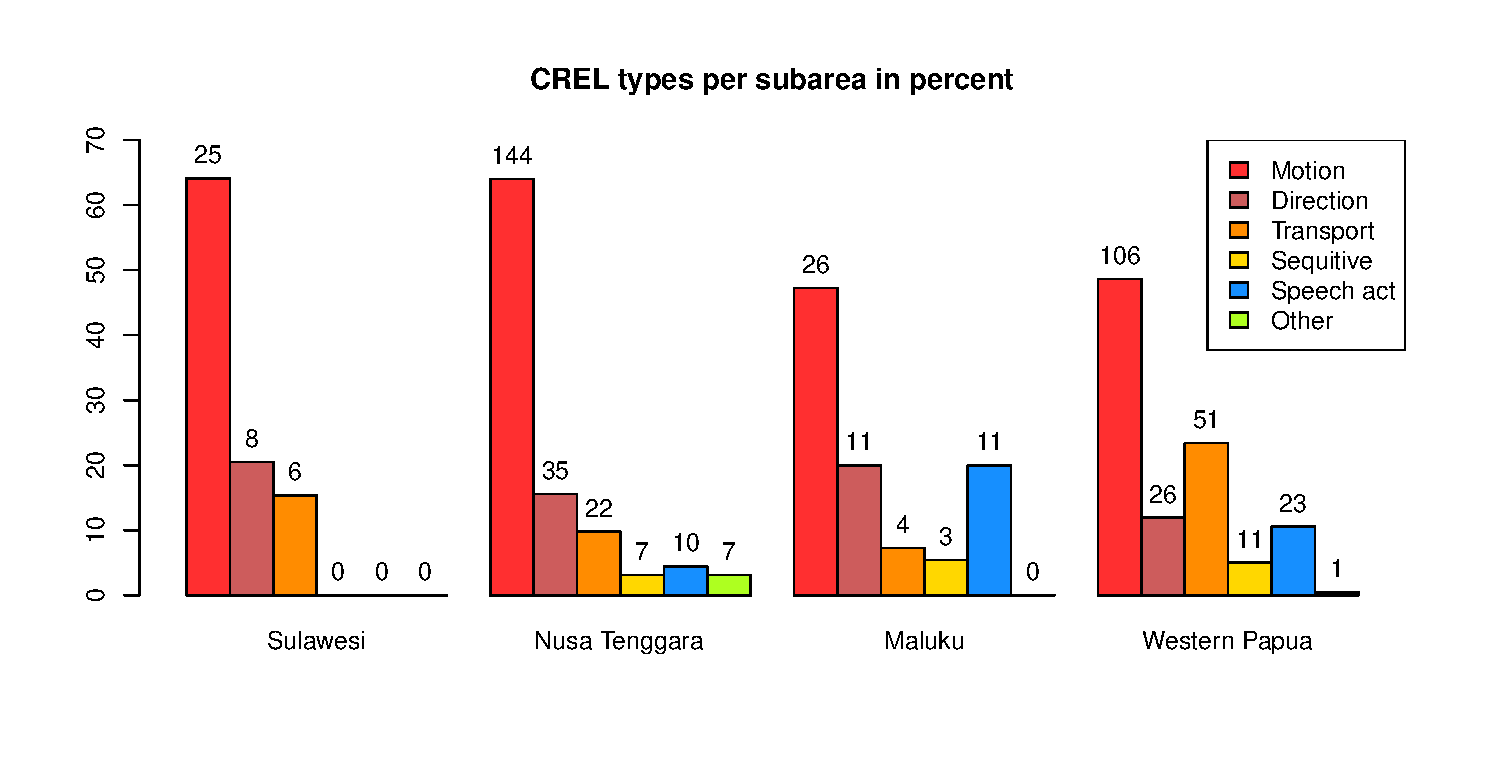
\includegraphics[width=.5\columnwidth]{figures/CREL_Group.eps}
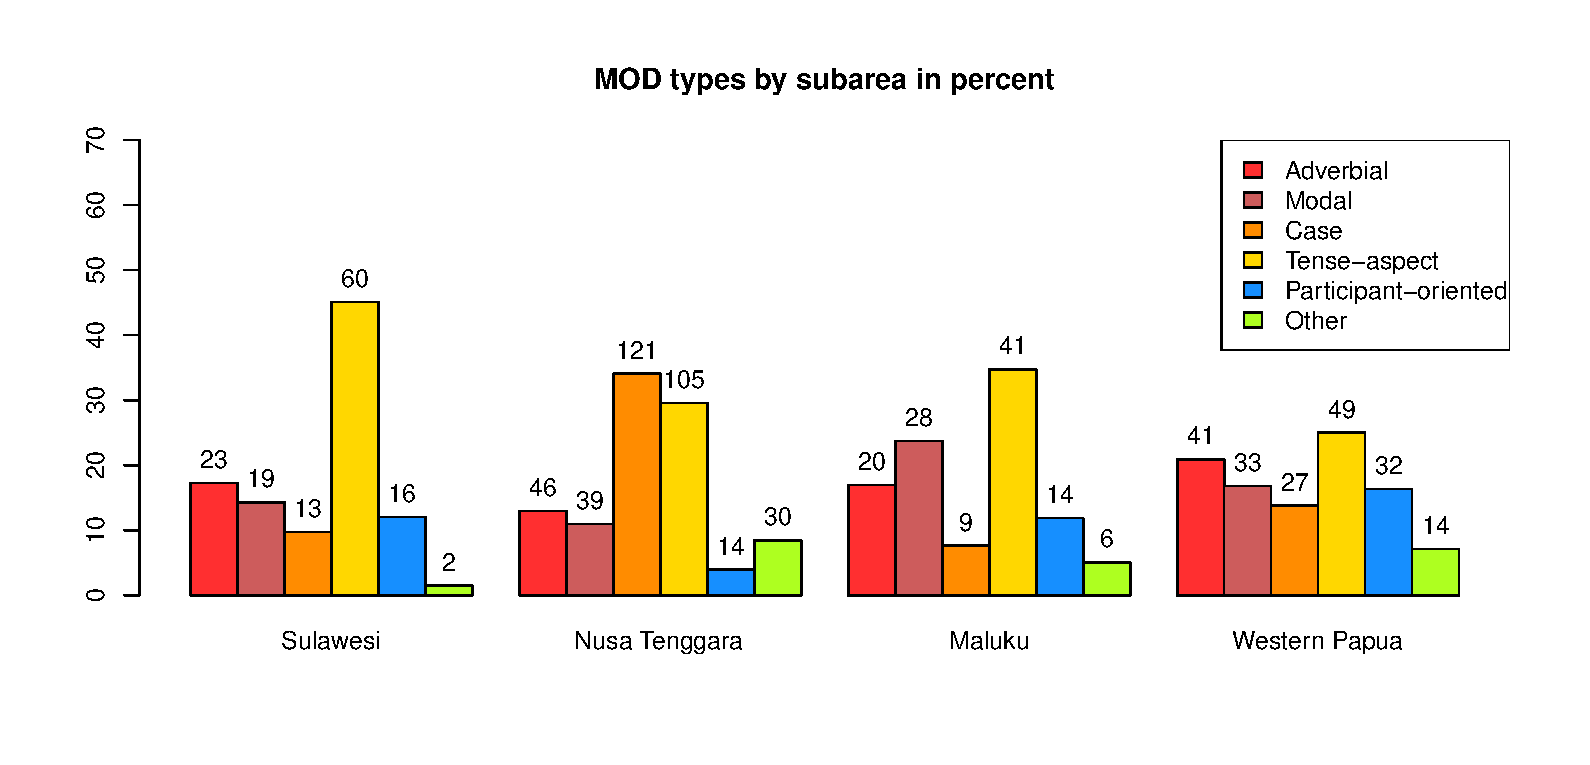
\includegraphics[width=.5\columnwidth]{figures/MOD_Group.eps}
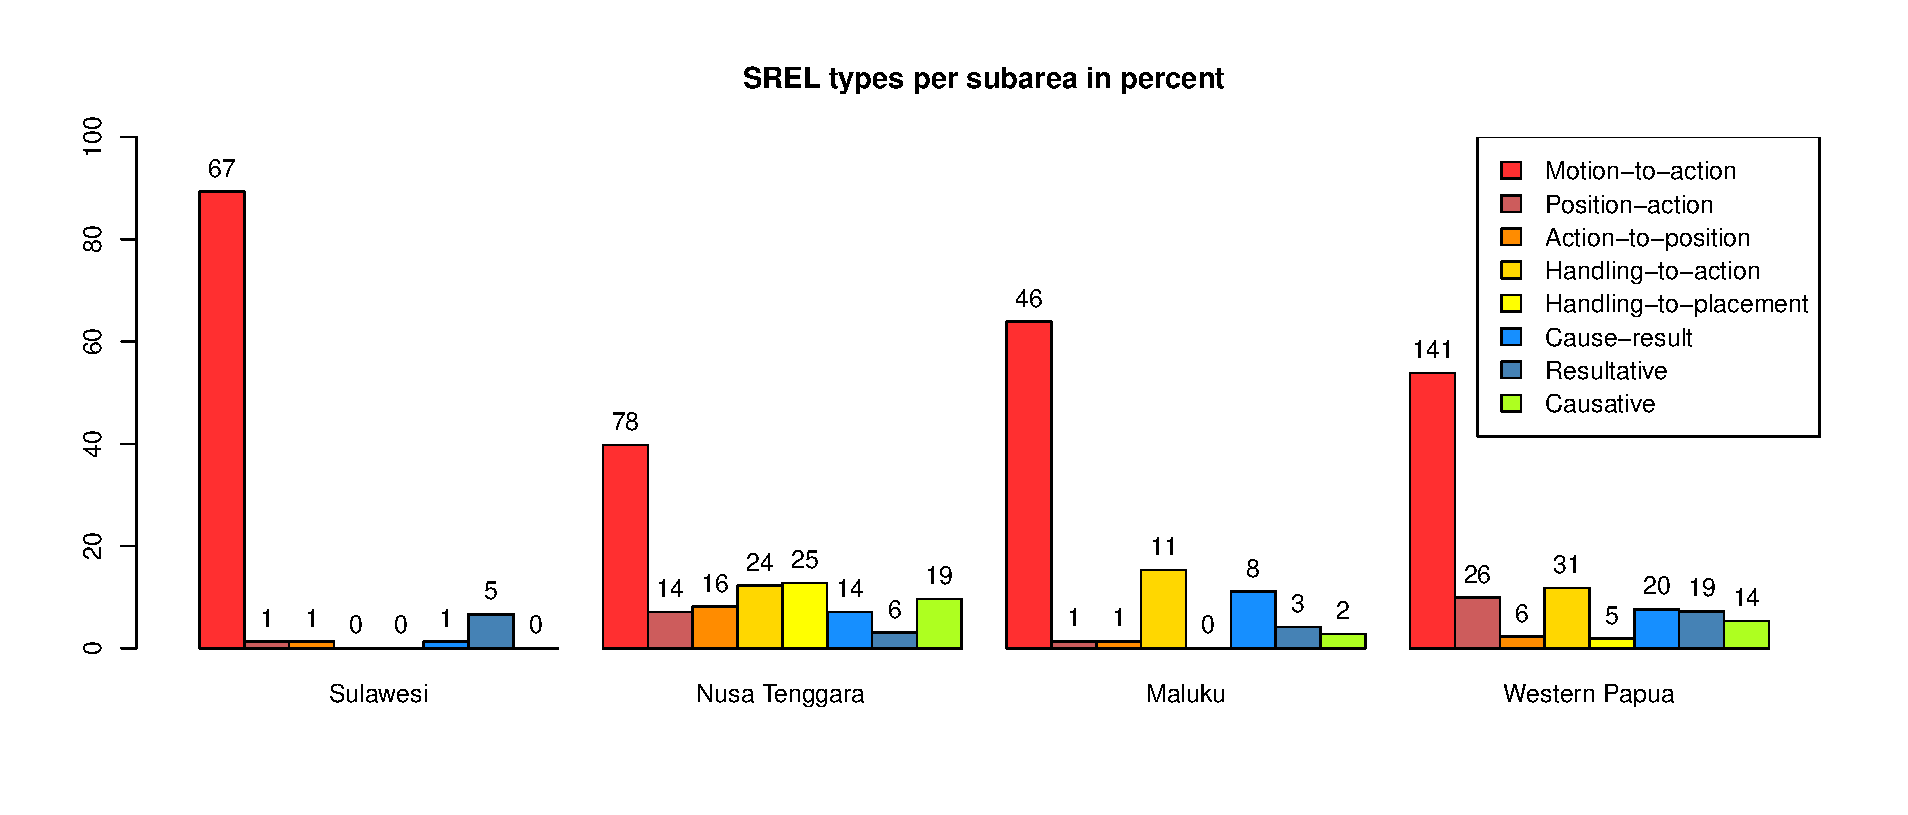
\includegraphics[width=.5\columnwidth]{figures/SREL_Group.eps}
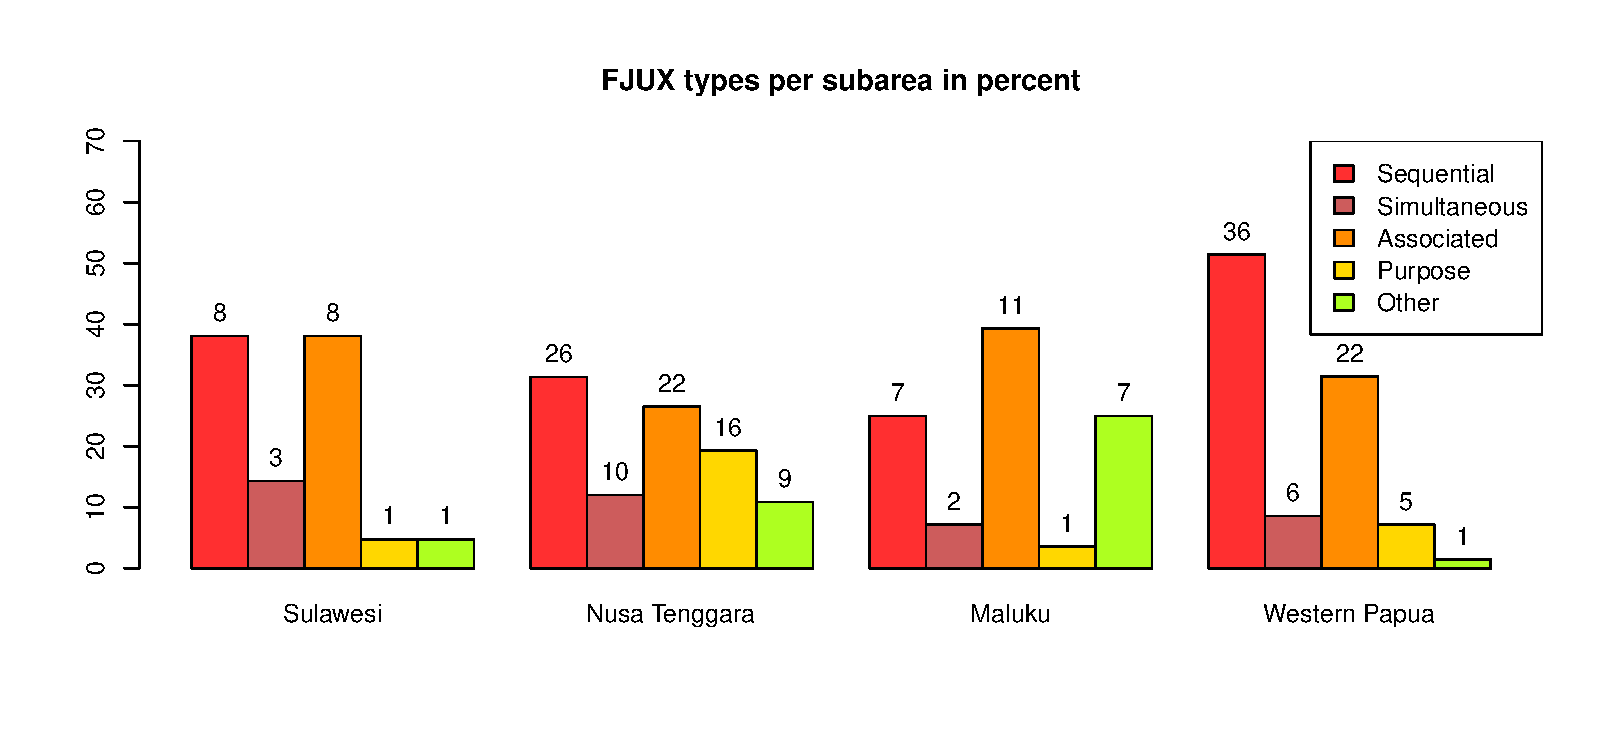
\includegraphics[width=.5\columnwidth]{figures/FJUX_group.eps}
\caption[MVCs per subarea in percent]{MVCs per subarea in percent. This is a composite of Figures \ref{fig:crel-group}, \ref{fig:mod-group}, \ref{fig:srel-group} and \ref{fig:fjux-group} from Chapter \ref{ch:constructions}. CREL = component-relating constructions, SREL = stage-relating constructions, MOD = modifying constructions, FJUX = free juxtaposition constructions. Numbers on top of the bars refer to the number of occurrences.}\label{fig:MVCs_subarea}
\end{minipage}
\end{sidewaysfigure}

In order to further explore the degree of MVC use across the EI languages let us have a look at another indicator. The data from the Figures in \ref{fig:MVCs_subarea} do not tell us how productively the formation of MVCs is integrated into the grammar of a given language. What I want to propose here is an examination of the number of different constructions attested per language. One could wonder whether languages which contribute many examples of MVCs show more attested constructions than languages with only peripherally developed means of MVC formation. Figure §\ref{fig:number_types} below is a calculation of all attested constructions per language as annotated in the EI sample (recall that MOD constructions have been collapsed into functional groups; here, I count all MOD constructions). Let us call this the ``D-score" of the EI languages, indicating the amount of constructional diversity found in each language. The numbers of the D-score are in part predictable from what has been said before. The peaks in the Papuan languages \ili{Abui}, \ili{Makalero}, and \ili{Maybrat} are not surprising as these languages have contributed many examples to the discussion in the previous chapters. Some other languages also contribute high numbers, such as the two corpus languages \ili{Waima'a} and \ili{Wooi}, or the Papuan language \ili{Tidore} from Maluku. Other peaks are more remarkable. The south-eastern Sulawesi languages all contribute more constructions than one might have expected from Figure §\ref{fig:MVCs_subarea} shown above. It is here that the wealth of MOD constructions in these languages becomes visible. With 25 attested constructions, \ili{Muna} shows the highest number among the Sulawesi languages, clearly contradicting the peripheral status of Sulawesi with regard to MVC use.

\begin{sidewaysfigure}
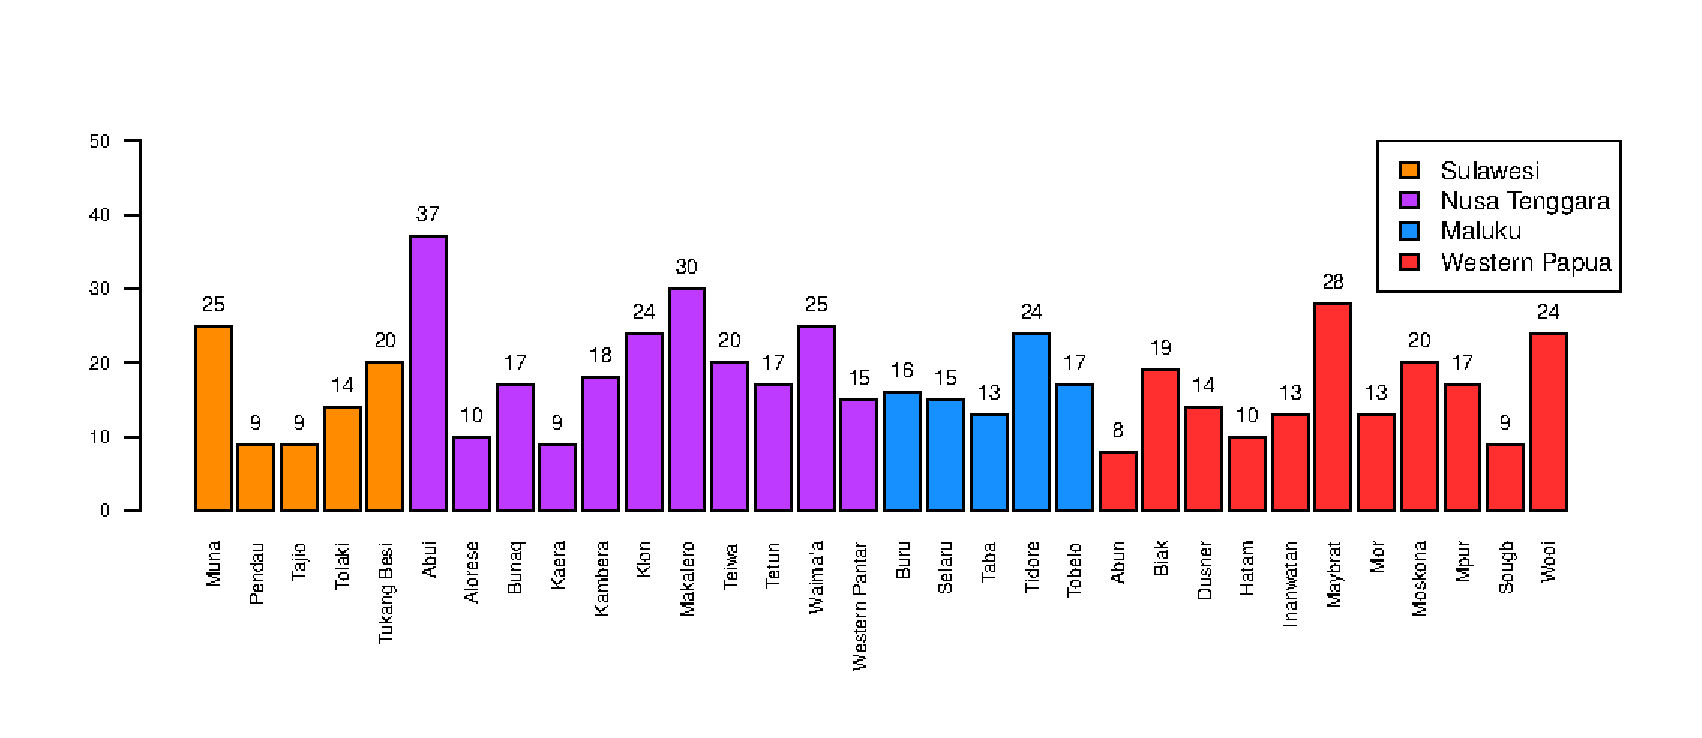
\includegraphics[width=\columnwidth]{figures/MVCs_languages_clean.eps}
\caption[Number of multi-verb constructions per language (``D-score")]{Number of multi-verb constructions per language (``D-score").}\label{fig:number_types}
\end{sidewaysfigure}

\largerpage[-1]
However, the calculation from \figref{fig:number_types} would only be representative if we assumed that the numbers were to show the complete inventory of constructions in use in the languages. This is, of course, not the case, since the source data material is limited. Therefore, we need to account for potential undetected constructions. For instance, both in \ili{Kaera} from the Nusa Tenggara subarea, and in \ili{Pendau} and \ili{Tajio} from Sulawesi, a total of nine different constructions is attested. One could draw the conclusion from these numbers that all three languages might have roughly the same degree of MVC use. However, a look at the amount of data points from each language reveals that \ili{Kaera} only contributed 24 data points, while \ili{Tajio} contributed 32 data points, and \ili{Pendau} contributed as many as 51. Therefore it appears more likely that, with 51 data points at hand as in \ili{Pendau}, the probability of detecting more constructions would be higher than with just 24 instances. Or put differently, the probability of undetected constructions is likely to grow smaller the more data points are added. This assumption holds true, of course, for all languages in the EI sample, which is why the total number of observation matters. The scatterplot in \figref{fig:constructions_tokens} below illustrates the ratio between the number of constructions and the number of data tokens in the EI languages. We can see that, as we move from left to right, the more data enter the game the more constructional types are found on average. Only when the amount of data becomes rather large does the number of detected constructions cease to grow. That is, while the trend is visible for virtually all languages for which published data were used, the two corpus languages, displayed on the far right, strongly suggest that, beyond a certain point, the bulk of constructions is detected and the likelihood of finding new constructions becomes small, no matter how much more data is added.

\begin{sidewaysfigure}
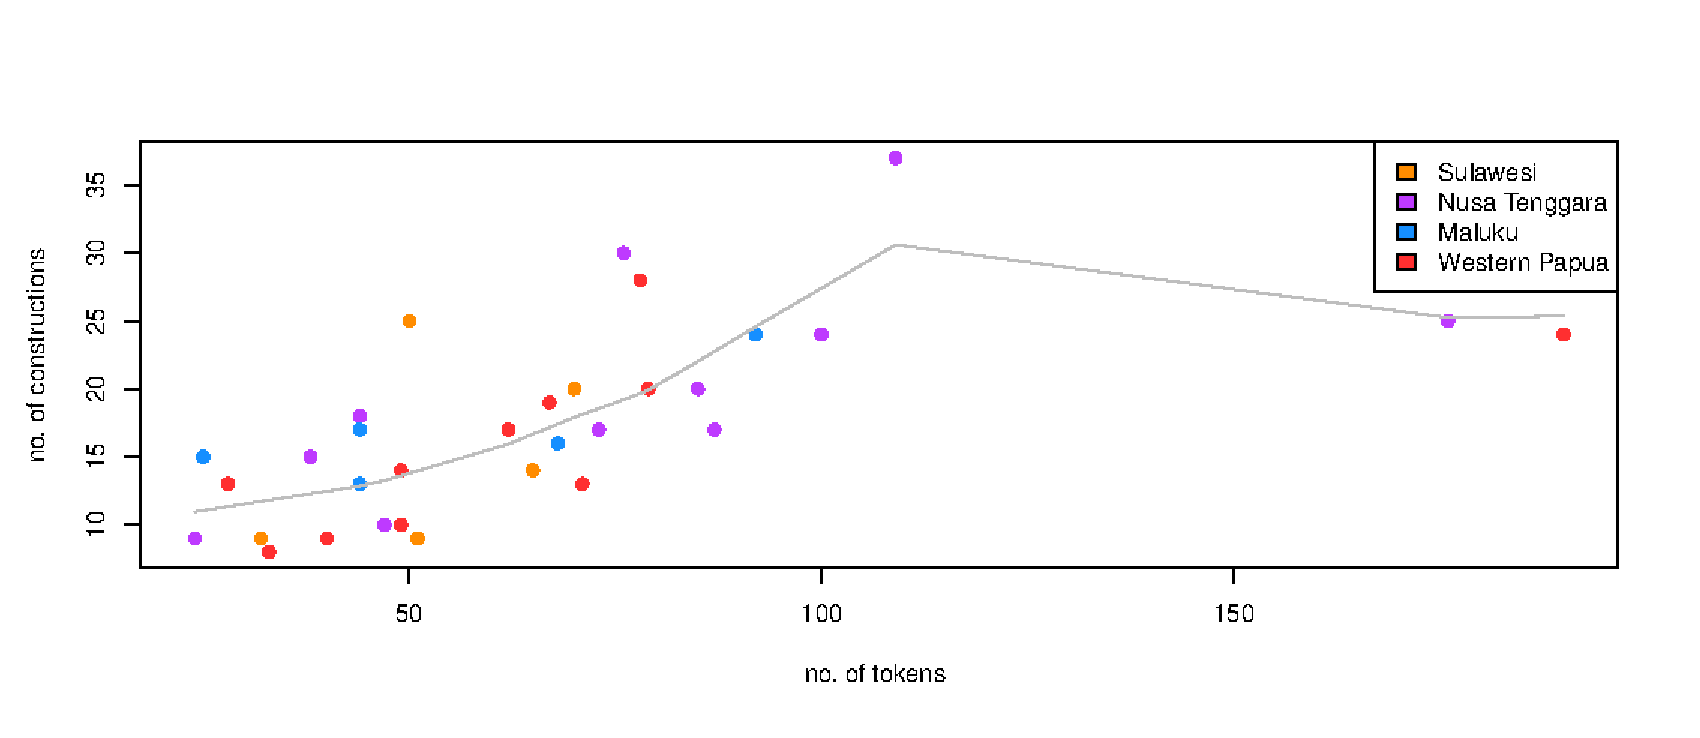
\includegraphics[width=\linewidth]{figures/constructions_tokens_clean.eps}
\caption[Correlation between number of constructions and number of tokens]{Correlation between number of constructions and number of tokens. Each dot represents one language from the EI sample. The dots to the far right belong to \ili{Waima'a} (violet) and \ili{Wooi} (red).}\label{fig:constructions_tokens}
\end{sidewaysfigure}

This observation leaves us with two potential factors that would need to be accounted for when we talk about MVC use. First, we have the number of attested constructions per language (n$_c$), i.e., a rough indicator of constructional diversity. And second, we have the number of observations or data tokens per language (n$_t$), i.e., a very rough measure of frequency of constructional use. \tabref{table:diversity_language} below returns the numbers of each factor. A simple way to relate these would be to divide the number of constructions by the number of tokens. The results are also displayed in \tabref{table:diversity_language}. This index provides the frequency of attested constructions per number of data tokens. For instance, \ili{Muna} has an index of 0.5, meaning that we end up with one detected construction for every two data tokens. This index, however, would only work well if the chance to detect new constructions would be the same across all languages. But this is clearly not the case. \ili{Selaru} is a good test case in this regard. \ili{Selaru} only contributed 25 data points to the sample. The reason for such a low number is that \ili{Selaru} predominantly uses a set of linkers, \textit{ti} and \textit{ma} (probably derived from motion verbs), to link verbs together. So, despite the fact that a whole grammar was searched for multi-verb constructions, very few were found. Thus, in this case we probably would not get significantly more constructions if we were to examine another source of \ili{Selaru} data. \tabref{table:diversity_language} in fact shows a higher value for \ili{Selaru} (0.6) than for, say, \ili{Abui} (0.34), although \ili{Abui} has the highest score of attested constructions (37). Note also that the corpus languages, \ili{Waima'a} and \ili{Wooi}, return extremely low numbers owing to the effect of a large corpus size outlined above. Such a frequency index clearly does not return reliable values. For the time being, I therefore stick to the number of constructions attested for each language, the D-score. In §\ref{sec:profile_use}, I will take up these numbers in order to present different profiles of MVC use throughout the EI area.

\begin{table}
\begin{footnotesize}
\begin{tabular}{l r r r}
  \lsptoprule
  \\
& n$_c$ & n$_t$ & $\frac{n_c}{n_t}$ \\ 
\\
  \hline
\ili{Muna}	& 25 &	50 &	0.5	 \\
\ili{Pendau}	& 9 &		51 &	0.18 \\
\ili{Tajio}	& 9 &		32 &	0.18 \\ 
\ili{Tolaki}	& 14 &	65 &	0.22 \\
\ili{Tukang Besi} &	20 &	70 &	0.29 \\ \hline
\ili{Abui}	& 37 &	109 &	0.34 \\
\ili{Alorese}	& 10 &	47 &	0.21 \\
\ili{Bunaq}	& 17 &	87 &	0.2	 \\
\ili{Kaera}	& 9 &		24 &	0.38 \\
\ili{Kambera}	& 18 &	44 &	0.41 \\
\ili{Klon}	& 24 &	100 &	0.24 \\
\ili{Makalero} &	30 &	76 &	0.39 \\
\ili{Teiwa}	& 20 &	85 &	0.24 \\
Tetun	& 17 &	73 &	0.23 \\
\ili{Waima'a}	& 25 &	176 &	0.14 \\
Western Pantar	& 15 &	38 &	0.39 \\ \hline
\ili{Buru}	& 16 &	68 &	0.24 \\
\ili{Selaru}	& 15 &	25 &	0.6	 \\
\ili{Taba}	& 13 &	44 &	0.3	 \\
\ili{Tidore}	& 24 &	92 &	0.26 \\
\ili{Tobelo}	& 17 &	44 &	0.39 \\ \hline
\ili{Abun}	& 8 &	33 &	0.24 \\
\ili{Biak}	& 19 &	67 &	0.28 \\
\ili{Dusner}	& 14 &	49 &	0.29 \\
\ili{Hatam}	& 10 &	49 &	0.2	 \\
\ili{Inanwatan}	& 13 &	28 &	0.46 \\
\ili{Maybrat}	& 28 &	78 &	0.36 \\
\ili{Mor}	& 13 &	71 &	0.18	 \\
\ili{Moskona}	& 20 &	79 &	0.25 \\
\ili{Mpur}	& 17 &	62 &	0.27 \\
\ili{Sougb}	& 9 &	40 &	0.23 \\
\ili{Wooi}	& 24 &	190 &	0.13 \\
\lspbottomrule
\end{tabular}
\end{footnotesize}
\caption[Diversity of multi-verb constructions per language]{Diversity of multi-verb constructions per language. n$_c$ = number of constructions, n$_t$ = number of tokens, $\frac{n_c}{n_t}$ = frequency index of constructions per number of tokens.}
\label{table:diversity_language}
\end{table}

\largerpage[-2]
In order to arrive at statistically relevant results one would need to normalise the number of tokens examined for each language. For instance, if for each language the same number of IPs defined on the basis of comparable boundary signals were explored in terms of n$_c$ and n$_t$, more accurate values could be obtained. This was for practical reasons beyond the scope of this book. What I want to propose here is that the D-score, i.e., the number of constructions found, can give at least a rough idea of the degree to which multi-verb constructions pervade the grammatical system of individual languages in Eastern Indonesia.\footnote{An anonymous reviewer pointed out that diversity of multi-verb constructions is not necessarily related to frequency of use. This is certainly true. What I intended to stress by comparing the number of constructions with the number of tokens is that the ratio between them is quite different across the individual languages, and that this may be meaningful. Recall that the sample does not only consist of data points deliberately provided in the source publications as examples of verb serialisation, but also of examples collected from sections and chapters totally unrelated to the discussion of verb serialisation. Languages with many data points but few attested constructions therefore appear to have a smaller repertoire of multi-verb constructions at their disposal, although this clearly needs further checking.}

\section{Hierarchy in MVCs} \label{sec:hierarchy}

Hierarchy in linguistic structure is typically accompanied by grammatical marking. Subordinate clauses, for instance, are flagged with non-finite or reduced verb morphology in many languages, or with grammatical formatives of some sort. The same applies to structures in which hierarchies could be expected, but where none are intended. Think of structures where conjunctive elements explicitly coordinate constituents that are on the same rank. Such devices are only sporadically encountered in Eastern Indonesia. Many EI languages lack an elaborate set of junctors, and \ili{Indonesian} loan junctors are sometimes used as a result of increased diglossia and exposure to regional Malay varieties. Native formatives that flag co- or subordination are rare in many EI languages. When there are morphological means to flag certain types of clause linkage, these overt constructions often replace MVCs. For instance, \ili{Kambera} has developed a proclitic \textit{pa=} denoting that the flagged constituent is controlled by a matrix clause (see \citealt[338ff.]{klamer1998grammar}). The proclitic is found, among others, in clause combinations that appear to function just like motion-to-action MVCs (but convey a purposive reading, or so it seems). Or, to mention another example, \ili{Abun} has a simultaneous-events construction flagged by the clitic \textit{=i}. The clitic is attached to clause-final position when two events happen at the same time \citep{berry1999}. Those cases have not been counted as simultaneous FJUX constructions, although functionally they bear some resemblance.

\largerpage[-1]
As MVCs are basically verb strings without grammatical marking, it comes as no suprise that very little has been written on hierarchies in MVCs, or in SVCs, for that matter. We have already seen in §\ref{sec:literature-mvcs} that \citet{enfield2008verbs} provides an insightful analysis of MVCs in \ili{Lao}, explicitly stating that many complex verb strings in \ili{Lao} may be dissected into mostly binary V$_1$-V$_2$ combinations. Reconsider example (\ref{lao1}) (here repeated as (\ref{lao_2})) from \ili{Lao} with six verbs in sequence.

\ea \label{lao_2}
\langinfo{Lao}{Tai-Kadai}{\citealt[83]{enfield2008verbs}}\\
\gll caw$^4$ lòòng$^2$ mèè$^4$ qaw$^3$ paj$^3$ hêt$^1$ kin$^3$ beng$^1$ \\
2\textsc{sg} try.out \textsc{ptl} take go make eat look \\
\glft `You go ahead and take (them) and try cooking (them)!'\\ 
\z

This utterance, as Enfield remarks, constitutes ``a single prosodically integrated unit", and \begin{quote}is no mere `string of verbs'. Such sequences in \ili{Lao} can be analysed in terms of nested (usually binary) relationships. In [the above] example [...], a left-headed complement-taking adverbial \textit{lòòng$^2$} `try out' combines with a right-marking adverbial \textit{beng$^1$} `look' in bracketing a complex verb phrase consisting of a `disposal' construction expressing focus on manipulation of the object (with the combination \textit{qaw$^3$-hêt$^1$} `take (and) do/make'), incorporating \textit{paj$^3$} `go' as an inner directional particle, in a purposive clause chain with \textit{kin$^3$} `eat'. The surface string of six contiguous verbs [...] is highly structured, yet there is little if any surface indication of such structure in the language. \citep[83]{enfield2008verbs}\end{quote}

The verb combinations from the \ili{Lao} example are strikingly similar to what we have seen in Chapter \ref{ch:constructions}, and the EI constructions may be stacked, or nested, in much the same way as in the \ili{Lao} string. Example (\ref{KYO001a}) from \ili{Klon} is certainly an extreme case of stacked MVCs in EI, but serves to illustrate how deep such recursive MVCs may extend. 

\ea \label{KYO001a}
\langinfo{Klon}{Papuan, TAP}{\citealt[140]{baird2008grammar}}\\
\gll pi brai brai lam agai nmei mi hos koh di, pi pa u-eel\\
\textsc{1}\textsc{nsg}.\textsc{in}.\textsc{act} slow slow walk go place be.at put finish first \textsc{1}\textsc{nsg}.\textsc{in}.\textsc{act} \textsc{1}\textsc{nsg}.\textsc{in}.\textsc{hor} \textsc{vi}-stop\\
\glft `We walked slowly, putting (them) in the place, then we rested, [...]'\\ 
\z

The MVC in (\ref{KYO001a}) comprises six verbs in sequence, up to \textit{koh} `finish' (disregarding the repetition of \textit{brai}). The verbs appear to fall into two groups: the first three verbs denote a motion event, slowly walking away from some discourse origo. Two motion verbs, \textit{lam} `walk' and \textit{agai} `go', are merged in order to form a \textsc{motion complex} MVC. The result of this merger is, on the next higher level, modified by \textit{brai} `slow'. I analysed such modifying relations as adverbial MOD MVCs in §\ref{sec:modification}. The verb triplet on the right hand side is internally structured in similar ways. Here it is two modifier verbs that attach at different levels. I assume that modification of \textit{hos} `put' by the locative verb \textit{mi} `be at' constitutes the inner MVC, and that the resulting case-marking MOD MVC is again modified by the aspectual verb \textit{koh}.\footnote{There are particular difficulties associated with interpreting the exact scope of modifier verbs, as has already become clear from the discussion in §\ref{sec:clauselevelmodification} on clause-level modification. In this case, an alternative analysis could treat the left-peripheral modifier \textit{brai} and the right-peripheral modifier \textit{koh} as having scope over the whole construction, resulting in a reading like `slowly, we walked away (and) put (them) in place (until) done'. I see no reason why this reading should not, in principle, be available as well, although a repetition of \textit{brai} seems more intimately connected to a process like walking rather than to an accomplishment like putting. Yet I assume that the preferred interpretation of such modifiers, especially in complex hard-to-parse structures like this one, is partial scope over neighbouring discernable event units.} At the topmost level we can recognise the by now familiar combination of a motion stage followed by an action stage, that is, the whole string is likely to be interpreted as a motion-to-action MVC. \figref{figure:eventschema_KYO001a} illustrates the internal structure of the whole sequence by applying the insights from Chapter \ref{ch:sem}. The event arguments, percolating upwards as the verbs combine to form event schemas on higher levels, spring from the dynamic verbs \textit{lam}, \textit{agai}, and \textit{hos}. The former two merge their event arguments, filling the event argument of the motion stage at the topmost level of the tree. The event argument from \textit{hos} percolates upwards and becomes the event argument of the action stage. The modifier verbs instead contribute empty event arguments that adapt to those of the matrix verbs.

\begin{sidewaysfigure}

\jtree[xunit=10em,yunit=2em]
\defbranch<shortleft>(1)(2.2)
\defbranch<shortright>(1)(-2.2)

\defstuff[a]{\multiline
{CLE -- motion-to-action (staged)}\cr
{\begin{scriptsize} [[ \textbf{do'} (we, \textbf{move'} (we, \textsc{path=\rnode{A3}{go}}, \textbf{walk'} (e$_{1=2}$, we))) \&  \textsc{slow} (e$_{1=2}$, we)] \& \end{scriptsize}}\cr
{\begin{scriptsize} [ \textsc{become} \textbf{do'} (we, \textbf{move'} (we, \textsc{path}, \textbf{put'} (e$_3$, we, (them)))) \&  \textsc{locative} (e$_3$, we) \& \textsc{finish} (e$_3$, we) ]]\end{scriptsize}}
\endmultiline}

\defstuff[b]{\multiline
{PLE -- adverbial modifying}\cr
{\begin{scriptsize}[ \textbf{do'} (we, \textbf{move'} (we, \textsc{path=go}, \textbf{walk'} (e$_{1=2}$, we))) \& \end{scriptsize}}\cr
{\begin{scriptsize} \textsc{\rnode{S4}{slow}} (\rnode{T4}{e$_{1=2}$}, we) ]\end{scriptsize}}
\endmultiline}

\defstuff[c]{\multiline
{PLE -- aspectual modifying}\cr
{\begin{scriptsize} [ \textsc{become} \textbf{do'} (we, \textbf{move'} (we, \textsc{path}, \textbf{put'} (e$_3$, we, (them)))) \& \end{scriptsize}}\cr
{\begin{scriptsize} \textsc{locative} (e$_3$, we) \& \textsc{\rnode{F4}{finish}} (\rnode{P7}{e$_3$}, we) ]\end{scriptsize}}
\endmultiline}

\defstuff[d]{\multiline
{PLE -- case modifying}\cr
{\begin{scriptsize} [ \textsc{become} \textbf{do'} (we, \textbf{move'} (we, \textsc{path}, \textbf{\rnode{P3}{put'}} (\rnode{P6}{e$_3$}, we, (them)))) \& \end{scriptsize}}\cr
{\begin{scriptsize} \textsc{\rnode{F2}{locative}} (\rnode{P5}{e$_3$}, we) ]\end{scriptsize}}
\endmultiline}

\defstuff[e]{\multiline
{PLE -- motion complex}\cr
{\begin{scriptsize}\textbf{do'} (we, \textbf{move'} (we, \textsc{path=\rnode{A3}{go}}, \textbf{\rnode{D4}{walk'}} (e$_{\rnode{C3}{1}=\rnode{B3}{2}}$, we)))\end{scriptsize}}
\endmultiline}

\! = {\stuff[a]}
<left>{\stuff[b]}!a ^<right>{\stuff[c]}
<left>[xunit=0.5em]{\stuff[d]}!b ^<right>[linestyle=dotted]{PLE}
<vert>{LLE}
<vert>{\textit{koh}}
{\begin{scriptsize} \textsc{\rnode{F3}{finish}} (e''', we)\end{scriptsize}}.

\!a = <left>[linestyle=dotted]{PLE}!c ^<right>[xunit=0.5em]{\stuff[e]}
<shortleft>{LLE}!d ^<shortright>{LLE}
<vert>[scaleby=1.6]{\textit{agai}}
{\begin{scriptsize} \textbf{do'} (we, \textbf{move'} (we, \textsc{path=\rnode{A2}{go}}, \textbf{go'} (\rnode{B2}{e$_2$}, we)))\end{scriptsize}}.

\!b = <shortleft>{LLE}!e ^<shortright>{LLE}
<vert>[scaleby=1.6]{\textit{hos}}
{\begin{scriptsize} \textsc{become} \textbf{do'} (we, \textbf{move'} (we, \textsc{path}, \textbf{\rnode{P2}{put'}} (\rnode{P4}{e$_3$}, we, (them))))\end{scriptsize}}.

\!c = <vert>{LLE}
<vert>{\textit{brai}}
{\begin{scriptsize} \textsc{\rnode{S3}{slow}} (e', we)\end{scriptsize}}.

\!d = <vert>{\textit{lam}}
{\begin{scriptsize} \textbf{do'} (we, \textbf{move'} (we, \textsc{path}, \textbf{\rnode{D1}{walk'}} (\rnode{B1}{e$_1$}, we)))\end{scriptsize}}.

\!e = <vert>{\textit{mi}}
{\begin{scriptsize} \textsc{\rnode{F1}{locative}} (e'', we)\end{scriptsize}}.

\psset{linestyle=dotted,angleA=45,angleB=-90,arrows=->}
\nccurve{A2}{A3} %von TRANS hoch zu TRANS-motion complex
\nccurve{B2}{B3} % von e2-go zu e2-motion complex
\nccurve{P2}{P3} % von put zu put-case mod
\nccurve{C3}{T4} %von motion complex = hoch zu e-slow
\nccurve{P4}{P5} % von e3-put zu e3-put-case mod
\nccurve{P4}{P6} % von e3-put zu e3-put-case mod
\nccurve{P6}{P7} % von e3-put zu e3-put-asp mod
\psset{linestyle=dotted,angleA=70,angleB=-45,arrows=->}
\nccurve{F3}{F4} %von finish hoch zu finish-aspec
\psset{linestyle=dotted,angleA=100,angleB=-100,arrows=->}
\nccurve{B1}{C3} %von e1-walk zu e1- motion complex
\nccurve{D1}{D4} %von walk hoch zu walk-motion complex
\nccurve{S3}{S4} %von slow zu adv-slow
\nccurve{F1}{F2} %von locative hoch zu case-locative
\endjtree

\caption[Event schema illustration of example (\ref{KYO001a})]{Illustration of the composite event schema of example (\ref{KYO001a}). LLE -- \textsc{lexeme-level event}, PLE -- \textsc{predicate-level event}, CLE -- \textsc{clause-level event}.}
\label{figure:eventschema_KYO001a}
\end{sidewaysfigure}

The challenge with such verbal interactions is to decide whether we are looking at structural dependencies as found, for instance, in many languages of Europe and Central Asia, or whether we are in fact dealing with paratactic formations, as \citep[151]{levinson2013recursion} remarks. Discussing recursion from a pragmatic perspective, Levinson points out that center-embedding, that is, a subordinate construction embedded on both sides into a matrix structure (ABBA), may be grammatically licit, but at a certain depth runs into severe parsing problems, so that center-embedding in oral language is practically capped at two levels deep (three in written language; \citealt[154]{levinson2013recursion}). While recursion by center-embedding is unambiguous and can be detected with ease, this is not the case for edge-recursion where dependencies are not structurally visible, as the embedded construction is only flanked on one side. It appears that recursion in EI MVCs is almost always edge-recursion, as cases of center-embedding are lacking. Take example (\ref{KYO001a}) again. Embedding takes place two levels deep. Starting from the motion-to-action matrix level, the motion stage branches off to the left, while the action stage branches off to the right. The resultant modifying MVCs then both exhibit edge-recursion directed towards the inner edge. Note, however, that we do not get a structure like ABA, say, (\textit{brai}(\textit{lam})\textit{agai}), so any lower-ranked MVC in example (\ref{KYO001a}) is a case of edge-recursion. The only cases of cross-serial dependencies in EI MVCs are found in motion complex MVCs from languages with AOV order which are modified by a locative verb marking the goal of the motion event. Example (\ref{Kaera_13}) from \ili{Kaera} is such a rare case. The two motion verbs flank the modifier verb in center position, but note that the modifying MVC is the matrix-level construction, as it modifies the whole motion complex, and not just one of the motion verbs. So, we are not in fact dealing with center-embedding here, but with discontinuous edge-recursion.

\ea \label{Kaera_13}
\langinfo{Kaera}{Papuan, TAP}{\citealt[138]{klamer2014kaera}}\\
\gll wer bir~bir ming, gang ekeng abang wang gi \\
sun \textsc{rdp}~run be 3\textsc{sg} climb.up village be go \\
\glft `At midday, she went up to the village.'\\ 
\z

Constraints on cross-serial dependencies in MVCs are in all likelihood due to obvious parsing problems. The longer a string of verbs gets, the more readings are possible. The lack of structural flagging is compensated by compiling such strings in paratactic patterns. Ease of parsing, however, does not preclude edge-recursion, and in compliance with the semantic approach outlined in chapter \ref{ch:sem}, we can identify a wealth of mostly binary verb--verb relationships within MVCs. Remarkably, internal structure of this sort is not observed in all constructional MVC families. Component-relating constructions have not been found with embedded MVC constructions, indicating their coherent one-staged semantic construal.

The fact that MVCs in EI can be stacked begs the question whether all EI languages allow stacking, and if so, to which extent? This question takes us back to the issue of MVC use and diversity in the EI region. As a hypothesis one may assume that languages with heavy use of MVCs show more MVC embedding than languages with only peripheral use of MVCs. As every construction in the EI sample has been annotated according to its hierarchical position, we can calculate the number of stacked MVCs by counting the number of matrix-level MVCs. \figref{fig:stacked} illustrates the number of stacked MVCs observed for each language.

\begin{sidewaysfigure}
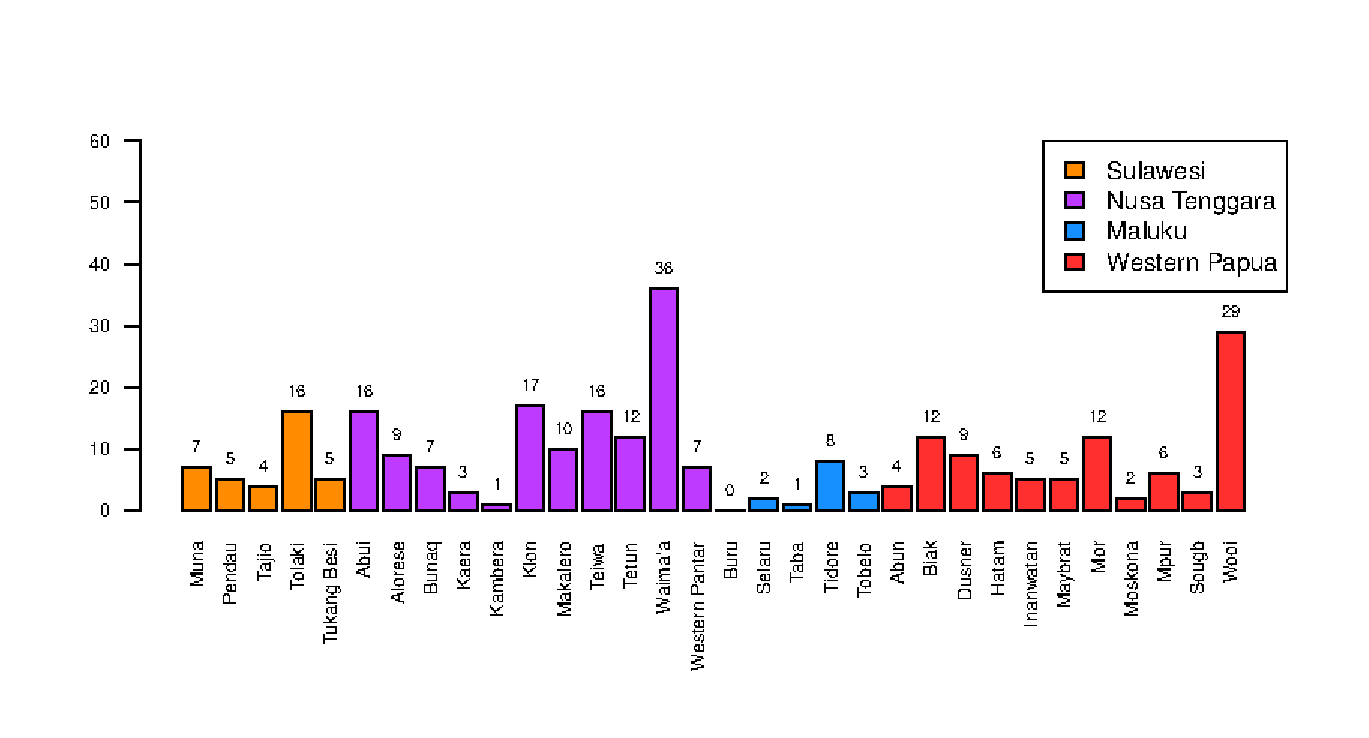
\includegraphics[width=\textwidth]{figures/number_stackedMVC_clean.eps}
\caption[Number of stacked MVCs per language]{Number of stacked MVCs per language.}\label{fig:stacked}
\end{sidewaysfigure}

Two observations arise from these numbers. First and counterintuitively, the amount of stacking does not necessarily correlate with the D-score from §\ref{sec:distribution}. While the Sulawesi group shows intermediate numbers of stacking, the numbers from the Maluku group are lower than expected. If we specifically compare the northern Sulawesi group \ili{Pendau} and \ili{Tajio} with the group of Austronesian Maluku languages, \ili{Buru}, \ili{Selaru} and \ili{Taba}, this distribution contradicts the trend from the D-score illustrated in \figref{fig:number_types}. And second, the two corpus languages, \ili{Waima'a} and \ili{Wooi}, fare especially well although they only show average D-score values. If the two languages with most data points score best, the distribution is obviously unbalanced. Therefore we need to take into account the total number of MVC observations per language (n$_t$). As in §\ref{sec:distribution}, I computed a frequency index by dividing the number of stacked MVCs by the total number of MVC observations. The results are illustrated in \figref{fig:complexity} below. As we are not dealing with a count of different types, as with the number of construction types in §\ref{sec:distribution}, but with the sum of observations of one particular value (=stacked), this index arguably is a slightly better predictor of MVC complexity than the frequency index from \tabref{table:diversity_language}. Therefore, I used this index instead of the mere number of stacked MVCs per language, as illustrated in \figref{fig:stacked}. I call it the C-score (complexity score), analogous to the D-score from the last section.

We can gather from the C-score values in \figref{fig:complexity} that the peaks of the two corpus languages are levelled out, but the same cannot be said for the values of the Sulawesi languages. Thus, in terms of internal MVC complexity, we can state that both the languages from Nusa Tenggara (with the exception of the western outlier \ili{Kambera}) and from Western Papua show the highest numbers of stacked MVCs in relation to the size of the data points considered. The Sulawesi languages, including the northern languages, also show rather high numbers of stacked MVCs. Finally and surprisingly, the Maluku languages lag behind in the use of complex MVCs (\ili{Selaru} has gained a little, but this, again, is probably a chance effect due to the low number of observations). 

\begin{sidewaysfigure}
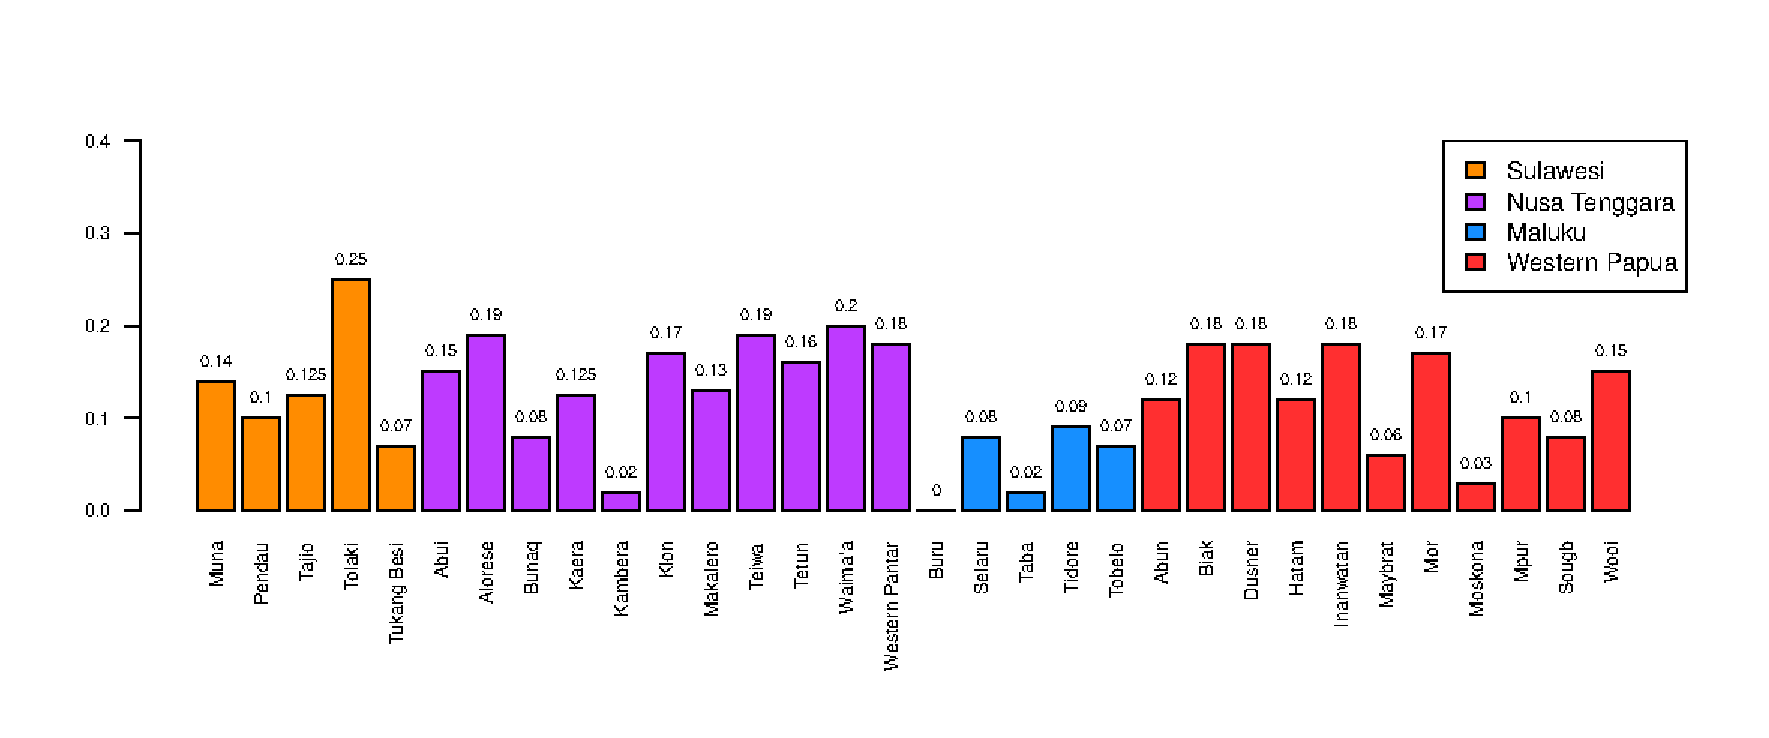
\includegraphics[width=\textwidth]{figures/index_MVCcomplexity_clean.eps}
\caption[Index of MVC complexity per language]{Index of MVC complexity per language (C-score). Explanation in the prose.}\label{fig:complexity}
\end{sidewaysfigure}

In the following section, I will combine the findings from this section and the previous one, and propose a tentative classification of the EI languages according to different profiles of MVC use.

\section{Linguistic profiles of MVC use} \label{sec:profile_use}

We have seen from the last two sections that the D-score (the number of constructions attested) and the C-score (derived from the frequency of complex MVCs relative to the number of observations available) both relate to MVC use in a given language. However, both values show opposing trends for some languages, and thus do not fit well in all cases. On the basis of the limited number of observations available from the EI sample there seems to be no simple \textit{ad hoc} solution that would resolve both factors into a single typology of languages, ranging from languages with little MVC use to languages with high usage. Let us therefore have another look at the C-score. The languages that scored highest in terms of constructional diversity (\ili{Abui}, \ili{Makalero}, \ili{Muna}, and \ili{Maybrat}) all have average C-values (at best; \ili{Maybrat} in fact has a very low C-score). Some  languages, on the other hand, that have low D-values fare surprisingly well. This is for example the case with \ili{Mor} from Western Papua, \ili{Alorese} and \ili{Kaera} from Nusa Tenggara, or \ili{Pendau} and \ili{Tajio} from Sulawesi. A closer inspection of these languages reveals that it is predominantly cases of motion-to-action MVCs with embedded motion CRELs in the motion slot (motion complex MVCs or transport MVCs) that cause higher numbers of stacked MVCs. Thus, most languages with high C-scores make good use of these constructions, and allow stacking in motion slots of motion-to-action. Given that both motion-to-action and motion complex MVCs are among the most frequent constructions found in the sample, the C-score is slightly skewed towards combinations of motion MVCs.

From what has been said, it seems reasonable to base a typology of MVC use on the D-score rather than on the C-score, and preference is therefore given to the D-score values. \tabref{table:profile_MVCuse} below outlines a typology of MVC use, and classifies the languages on the basis of their D-score values. I distinguish between four profiles in the EI region: languages with little use of MVCs (rank I), languages with moderate use (rank II), and languages with extensive use (rank III). To these we may add another language profile: languages that do not make use of MVCs altogether (rank 0). Rank 0 languages do not show up in the EI sample because all sample languages were checked for MVC use beforehand, and languages without signs of MVC use had been excluded. The threshold values to define the profiles are derived from the D-score and are largely chosen at arbitrary points. In order to be able to include the C-score results, I computed the C-score mean, which is 0.12, and compared it to the C-score values of the languages. Languages that strongly deviate from this mean are allowed to move up or down one rank. To this end, I computed the standard deviation from the C-score mean ($\pm 0.06$) and defined it as the threshold beyond which a given language would move up or down one rank ($0.12 \pm 0.06$). Any language with a C-score less than 0.06 would be ranked lower, and any language with a C-score greater than 0.18 would be ranked higher. So, for instance, as the C-score of \ili{Kambera} is only 0.02 the language is ranked down from the moderate use profile to the little use profile. Changes in ranking are displayed by the symbols $\uparrow$ and $\downarrow$, respectively. Note that in the case of \ili{Taba} I made one exception to this, not allowing a rank I language to move downwards to rank 0. This is because a language that does obviously use MVCs of quite different sorts can hardly be classified as having no MVC use at all. \tabref{table:profile_MVCuse} illustrates the different profiles, and sorts the EI languages according to the procedure just discussed.

\begin{table}
\begin{footnotesize}
\begin{tabular}{r l l p{5cm} }
\lsptoprule
Rank & Profile & D-score threshold & Languages \\
 \\ 
\hline
 Rank III & extensive MVC use & $D > 24 $ & \ili{Muna}, \ili{Abui}, \ili{Makalero}, \ili{Teiwa}$\uparrow$, \ili{Waima'a}, \ili{Maybrat} \\ 
\hline 
Rank II & moderate MVC use & $  15 \leq D \geq 24 $ & \ili{Tolaki}$\uparrow$, \ili{Tukang Besi}, \ili{Alorese}$\uparrow$, \ili{Bunaq}, \ili{Klon}, Tetun, Western Pantar, \ili{Selaru}, \ili{Tidore}, \ili{Tobelo}, \ili{Biak}, \ili{Mpur}, \ili{Wooi} \\
\hline
Rank I & little MVC use & $ 5 \leq D \geq 14 $  & \ili{Pendau}, \ili{Tajio}, \ili{Kaera}, \ili{Kambera}$\downarrow$, \ili{Buru}$\downarrow$, \ili{Taba}($\downarrow$), \ili{Abun}, \ili{Dusner}, \ili{Hatam}, \ili{Inanwatan}, \ili{Mor}, \ili{Moskona}$\downarrow$, \ili{Sougb} \\
\hline 
Rank 0 & (almost) no MVC use & $ D < 5 $ & \textit{none in EI sample} \\    
\lspbottomrule 
\end{tabular}
\end{footnotesize}
\caption[Linguistic profiles of MVC use]{Linguistic profiles of MVC use. Languages with a C-score below or above standard deviation ($D < 0.06$ or $D > 0.18$) are ranked lower or higher. Reranked languages are marked with $\downarrow$ and $\uparrow$, respectively. \ili{Taba} was chosen to be left in rank I and not moved down (indicated by the brackets).}
\label{table:profile_MVCuse} 
\end{table}

A comparison of the results from \tabref{table:profile_MVCuse} with the D-score values shows that all four languages that scored highest reappear in the `extensive use' profile: \ili{Muna}, \ili{Abui}, \ili{Makalero}, and \ili{Maybrat}. One further language from Nusa Tenggara, \ili{Teiwa}, has been promoted upwards due to high C-scores. Most other EI languages are classified as showing moderate MVC use (n=15), while another sizeable group are ranked as ``little MVC use" (n=13). As might be predicted, among these rank I languages, we predominantly find languages from the periphery of the EI region: the two northern Sulawesi languages \ili{Pendau} and \ili{Tajio} belong to this group, as well as the western outlier \ili{Kambera} from the Nusa Tenggara subarea, and also the Austronesian languages \ili{Dusner} and \ili{Mor} located in the southern part of Cenderawasih Bay (Western Papua group). 

\begin{sidewaysfigure}
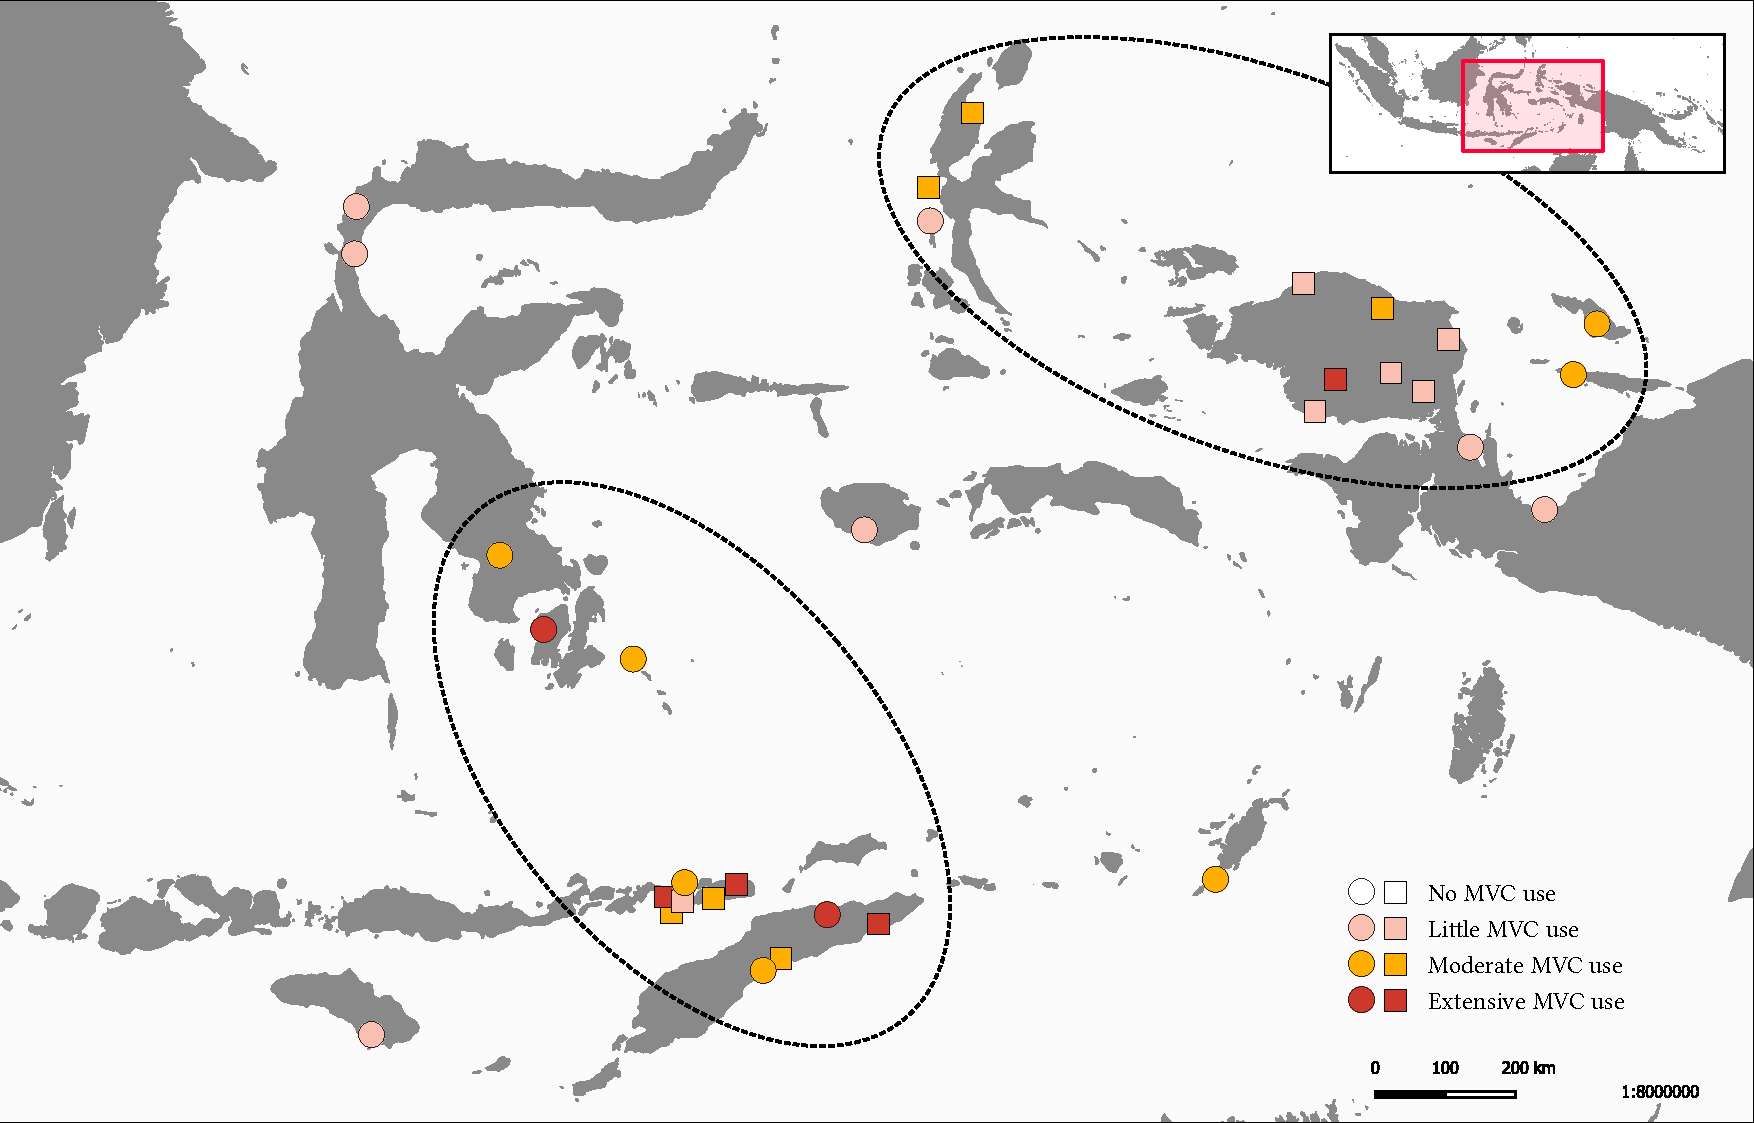
\includegraphics[width=\textwidth]{figures/languages_mvcuse.pdf}
\caption[Geographical distribution of linguistic profiles of MVC use across Eastern Indonesia]{Geographical distribution of linguistic profiles of MVC use across Eastern Indonesia. Languages are grouped into Austronesian (circles) and Papuan (squares). The colours designate the four linguistic profiles from \tabref{table:profile_MVCuse}. Two Sulawesi languages, \ili{Totoli} and \ili{Makassarese}, have been added as outgroup examples, and are good candidates for the rank 0 profile. Potential core areas of MVC use are highlighted by dotted outlines.}\label{fig:map_profiles}
\end{sidewaysfigure}

\figref{fig:map_profiles} is a visualisation of the geographical distribution of the different linguistic profiles across Eastern Indonesia. I also include two outgroup languages that I had given a cursory glance when compiling the sample (but dismissed due to a lack of attested MVCs). Both languages belong to the Western-Malayo-Polynesian branch of Austronesian, and are spoken in Sulawesi. \ili{Totoli}, located on the Minahasa Peninsula at Tolitoli Bay in northern Sulawesi, was documented by another DoBeS language documentation project \citep{leto2012totoli}, and is related to \ili{Pendau} and \ili{Tajio}. \ili{Makassarese} belongs to the South-Sulawesi branch of WMP and is spoken in Makassar and its vicinity on the tip of the South Peninsula \citep{jukes2005makassar, jukes2006makassarese}. For \ili{Totoli}, I explored two pear story narrations from the \ili{Totoli} corpus. For \ili{Makassarese} I searched the publications including one appended text, but in both cases only very weak traces of MVC use could been found (basically pseudo-modal verb constructions involving \textsc{want} and \textsc{can} verbs, as well as a handful of examples that might be interpreted as motion-to-action). Thus, for the time being I tentatively assume that both \ili{Totoli} and \ili{Makassarese} constitute examples of the ``no use" profile. If any dividing line is to be drawn between a Sprachbund area where the languages converge on using MVCs to at least some extent, and adjacent areas where MVCs play no or almost no role, it would in all likelihood run somewhere through Sulawesi.

From the distribution of rank II and rank III languages, we can identify two major ``hotspots" of MVC use in EI: a southern core area appears to include the Timor-Alor-Pantar complex of languages, spoken on Timor and neighbouring islands. It is not only the Papuan TAP languages that conform to a high MVC use, but also the Austronesian neighbours like \ili{Waima'a} and Tetun (and also, to a lesser degree, \ili{Alorese}). This core area probably radiates out into south-eastern Sulawesi and includes the seafaring language communities of \ili{Muna} and \ili{Tukang Besi} with their long-standing history as traders \citep{donohue1999}. A second, though less pronounced, core area of MVC use can be seen stretching from the Bird's Head to Northern Halmahera, roughly covering the West Papuan zone of influence \textit{sensu} \citet{reesink2005west}. Here as well, we can observe that the Austronesian languages spoken in the same area are almost all classified as showing at least moderate MVC use. \ili{Taba} is ranked lower, but still shows a sufficient amount of MVC use. The region between these MVC hotspots, the southern Moluccas, is clearly underrepresented in the sample, so that no real conclusion can be drawn. Yet judging from the two languages included in the sample it seems that the use of MVCs is indeed lower throughout this area. Recall that \ili{Selaru} only yielded very few data points, so that the classification into rank II might be biased by a dearth of total observations. In general, it is evident that MVC use is specifically high in areas with Papuan presence. This could be taken to support the assumption that MVC formation is a Papuan trait rather than Austronesian, and that Austronesian languages with regular exposure to Papuan language communities might be prone to showing higher degrees of MVC use than more peripheral Austronesian languages.

\section{MVC formation: A view from discourse analysis} \label{sec:discourse}

A last issue to which I want to turn briefly is the prosody of MVCs as seen from a discourse perspective. I have argued in \sectref{sec:prosodic} and elsewhere that a strict match between syntactic units and prosodic units is implausible. Assuming that prosody cues the existence of grammatical constructions can only be a rough heuristic in order to delimit a certain set of observations thought to constitute a phenomenon of its own. I followed this heuristic while collating the EI data material, and assumed for the sake of crosslinguistic comparability that MVCs in EI are necessarily coherent prosodic units, with an unbroken f$_0$ contour and clear boundary signals to it.

This assumption only becomes problematic at the point where we start to infer syntactic boundaries from prosodic ones. In this section, I want to present some data, mostly from the two corpus languages \ili{Waima'a} and \ili{Wooi}, that illustrate the fallacy of such an inference, at least for the constructional families that correlate two event stages (that is, SREL and FJUX constructions). Data from published sources seldom contain contextual information. Examples of SVCs presented in grammatical descriptions are often chunks of utterances, IPs at best, that are stripped of their discourse relations, and isolated from their preceding units. Information on how such structures form as part of discourse practices is largely missing. Looking into natural speech data from \ili{Wooi} and \ili{Waima'a} suggests that such ``bare" examples from grammars and research papers may obscure the functions that MVCs possess in discourse development, and, as a consequence, their coming into being. Two-staged MVCs often do not appear to be formed and produced on the spot, but rather build up incrementally. Consider the following stretch of utterances from a \ili{Wooi} explanatory describing the burning of, and planting of seedlings in, a forest garden.  

\ea \label{Wooi_gardening1}
\langinfo{Wooi}{Austronesian, SHWNG}{gardening\_exp1}\\
\ea 
\glll enuin da ve etiri ra kekavi \\
e-nuing ra ve e-iri ra $<$i$>$kakavi \\
\textsc{4}-burn until \textsc{purp} \textsc{4}-clear until $<$\textsc{3}\textsc{sg}$>$clean \\
\glft `It is burned for clearing (the spot) until it is empty' \\ 
\ex
\gll terus yo \\
then \textsc{fill} \\
\glft `then' \\ 
\ex
\glll a: tantanani \\
a: ta-tanang-i \\
\textsc{fill} \textsc{1}\textsc{pl}.\textsc{in}-plant-\textsc{obj}.\textsc{sg} \\
\glft `we plant it (with seedlings)' \\ 
\ex
\glll tatiri ra kekavi tantanani mara interi \\ 
ta-iri ra $<$i$>$kakavi ta-tanang-i mara interi \\
\textsc{1}\textsc{pl}.\textsc{in}-clear until $<$\textsc{3}\textsc{sg}$>$clean \textsc{1}\textsc{pl}.\textsc{in}-plant-\textsc{obj}.\textsc{sg} \textsc{top} then \\
\glft `we clear it until clean (and) plant it.'\\ 
\z
\z

The example consists of three utterances (and a regulatory filler), each separated by a final LH boundary tone and lengthening of the penultimate syllable. The first and the third intonation phrase each serve to establish one event. Both construals are in fact quite different. In the first IP an impersonal ``fourth person" subject is used. In the third IP, the speaker then shifts to a first person subject. The last IP finally combines the two events just established by wrapping it all up into what looks like a summary of the paragraph. While the verbs each come to stand at the very end of the first IPs, and articulation slows down at the lengthened segments, in the summarising IP they reappear in non-final position, with accelerated articulation speed and a reduction of word-final syllables. This directly reflects the difference in topicality. The event line is now well introduced and salient, so that the speaker can compress both event stages into one overall IP, and turn the whole sequence into a sentential topic marked by \textit{mara}. \figref{fig:gardening_pitch} illustrates the prosodic properties of example (\ref{Wooi_gardening1}).\todo{changed fig size to fit page}

\begin{figure}
%	\centering orig 1.8\textwidth
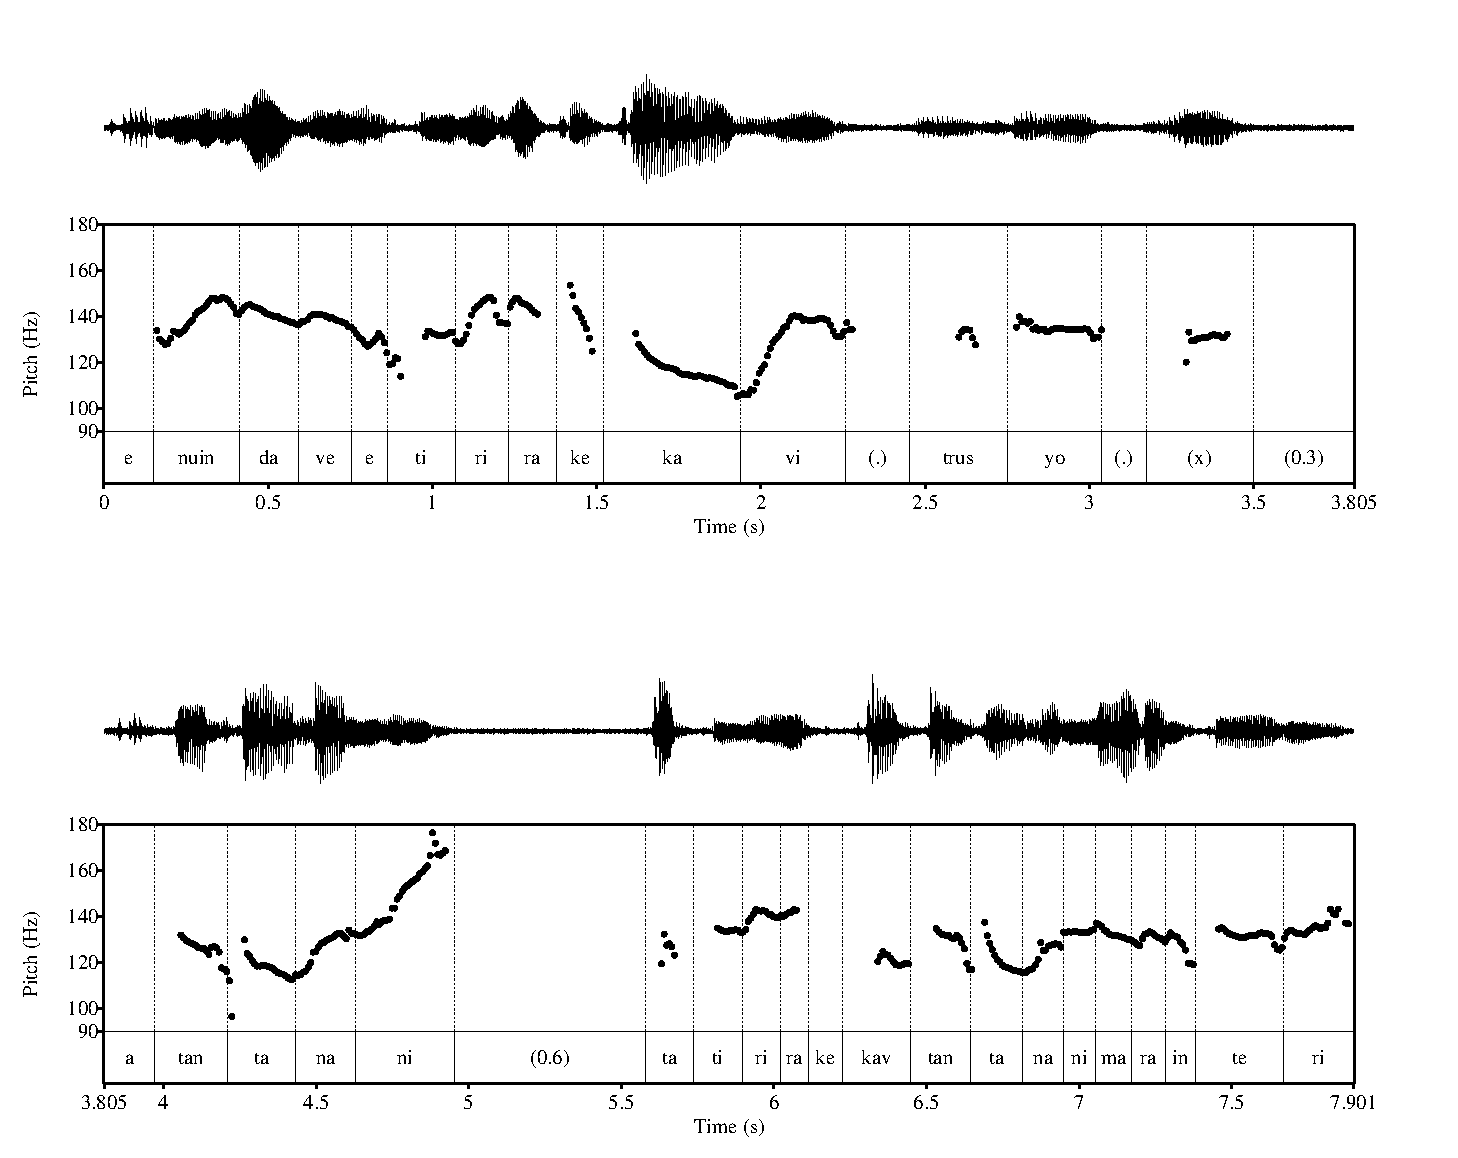
\includegraphics[width=1\textwidth]{figures/gardening1_burnplant.eps} 
\caption{F$_0$ contour of example (\ref{Wooi_gardening1})}\label{fig:gardening_pitch}
\end{figure}

Such incremental build-ups of compressed known information is in fact well known in Papuan linguistics. Papuan languages show strong preferences for a set of strategies that are crucial in discourse structuring and development \citep{devries2005towards, devries2006areal}. Three strategies are highly relevant in our context, and are found to actively shape the discourse structure in many EI languages (Papuan as well as Austronesian). 

Thematisation refers to the establishment of referents, locations and other discourse objects forming the inventory of participants for the text to follow \citep{heeschen1998eipo, devries2006areal}. Typical contexts of thematising are the beginning of texts, or at points where a break in the story-line occurs, and new discourse participants have to be introduced. Thematising often results in ``a paratactic series of thematic or setting constituents" \citep[814]{devries2006areal}. But thematisation is also evident from contexts  in which the story-line is progressing. In example (\ref{Wooi_gardening1}) from \ili{Wooi}, the event construals established in the preceding IPs are not only compressed into a summarising IP, but the whole string of verbal constituents is marked as a sentential topic, which serves as the backdrop for the following utterances. The topic marker \textit{mara} in \ili{Wooi} permits the wrapping of different verbal constituents into structures of unspecified length and complexity. It is thus not a topicaliser of clauses, but rather of sentences.

Distribution (of nominals) is a second major discourse strategy in Papuan languages also heavily shaping the way Papuan texts are organised \citep{devries2005towards, devries2006areal}. We have already seen examples of distributive strategies in EI languages. The \ili{Makalero} verb system is a good example to begin with. Recall from §\ref{sec:nus} that \ili{Makalero} prevents ditransitive argument configurations. A main verb provides one object slot which can be filled by a direct object argument, or by an adjunct complement \citep{huber2011}. Ditransitive argument frames are resolved by using multi-verb strings instead. As we have seen, \textit{mei} `take' has developed into a lightverb licensing further arguments into the event schema. Related strategies are found in other TAP languages, for instance in transfer constructions consisting of multi-verb strings \citep{klamer2012development}. Of course, \ili{Makalero} is a rather extreme case where a discourse-based tendency has been conventionalised into grammatical rules. But, as \citet[813]{devries2006areal} put it, \begin{quote}[i]f there must be nominals, Papuan speakers [...] try to have no more than one nominal modifying the verb in the clause, and no more than one modifying element in the nominal phrase.\end{quote} This strategy results in structures that are rich in verbs, but where nominals are few, and sparsely distributed across MVCs, verb chains, and related mechanisms. Although distributive strategies are strongly associated with Papuan languages, Austronesian languages from the EI region show similar patterns. In isolating languages of Timor, such as \ili{Waima'a} or \ili{Tetun Fehan}, nominals are often dropped when participants are known or inferable from the discourse context, resulting in strings of verbs with only occasional occurrence of nominal expressions. Distributing nominals across utterances can also influence the formation of MVCs, as the following example from \ili{Wooi} illustrates.

\ea \label{Wooi_leaf}
\langinfo{Wooi}{Austronesian, SHWNG}{MANTERA\_magic charms}\\
\ea
\glll ka: ariaung vati kori ma \\
kaynteri ariaung vati $\emptyset$-ko=i ma \\
next leaf \textsc{det}:\textsc{sg} \textsc{1}\textsc{sg}-take-\textsc{obj}.\textsc{sg} come \\
\glft `The leaf, I carry hither' \\ 
\ex
\glll kor ma honi ho botol \\
$\emptyset$-ko=i ma $\emptyset$-honi ho botol \\
\textsc{1}\textsc{sg}-take-\textsc{obj}.\textsc{sg} come \textsc{1}\textsc{sg}-fill \textsc{dir} bottle \\
\glft `I carry it hither and put it into a bottle.'\\
\z
\z

The short sequence of two utterances in (\ref{Wooi_leaf}) is part of an explanatory text on how to turn leaves from a particular tree into a magic charm. The leaf is established as a discourse participant in the first IP. \textit{Ariaung vati} is the first mention of the leaf in the text, and placed in preposed topic position before the verb\footnote{Topical fronting of nominals triggers the use of the resumptive clitic on the predicate.}. The second IP then serves to link the event depiction from the previous IP to the action coming next in the procedure. Instead of repeating the nominal, the leaf is referred to by use of the resumptive object clitic \textit{=i}, and another nominal, \textit{botol}, is used by the following verb to introduce a new participant. The MVC resulting from the linking process belongs to the motion-to-action construction. Note that it is only the two-stage SREL construction that is shaped by means of the distributive strategy. The component-relating MVC \textit{kori ma} is produced on the spot. This seems to be a general difference between CREL and SREL MVCs. I have never come across a single example of a component-relating construction that would emerge incrementally across two or more IPs.

Example (\ref{Wooi_leaf}) also illustrates another pervasive discourse strategy in the languages of New Guinea. I already mentioned that the content of the first IP is repeated in the second, and linked to the next predication. This pattern has come to be known as tail-head linkage, or recapitulative linkage in Papuan linguistics \citep{devries2005towards, devries2006areal}. Repeated structures such as the carrying from example (\ref{Wooi_leaf}) form the ``tail" of the next clause (the ``head"). Consider the paragraph in example (\ref{Korafe}) from \ili{Korafe}, a Trans-New-Guinea language from PNG \citep{farr1999interface}.

\ea \label{Korafe}
\langinfo{Korafe}{Papuan}{\citealt[816]{devries2006areal}, quoted from \citealt[338]{farr1999interface}}\\
\ea
\gll vose bu jigh-ir-iri karaje mindi ambududuru-seri \\
descend.I get.I hold-remain-\textsc{sim}.\textsc{rls}.3\textsc{sg}.\textsc{ds} salt.water eat.I die.II-\textsc{dpst}.3\textsc{pl}.\textsc{fn} \\
\glft `It descended and held them while they drowned (lit. ate salt water and died).' \\ 
\ex
\gll amb-ero gi-do bebesuge-tiri eroru-seri \\
die.I-\textsc{seq}.\textsc{rls}.3\textsc{pl}.\textsc{ds} see.I-\textsc{seq}.\textsc{ss} open.up.\textsc{rdp}.I-\textsc{seq}.\textsc{rls}.3\textsc{sg}.\textsc{ds} arise.II-\textsc{dpst}.3\textsc{pl}.\textsc{fn} \\
\glft `Seeing that they had died, it opened out its tentacles and they floated up.' \\ 
\ex
\gll ere-do, feeghe viti-f-era \\ 
arise.I-\textsc{seq}.\textsc{ss} float.I ascend.I-come.\textsc{dur}-\textsc{seq}.\textsc{rls}.\textsc{pst}.3\textsc{pl}.\textsc{ss} \\
\glft `Their bodies arose, floated and came up and...' \\ 
\z
\z

\ili{Korafe} is a clause-chaining language and employs suffixes on the medial verbs in order to facilitate subject tracking. Example (\ref{Korafe}) consists of three clause-chains. At the beginning of each new chain, the finite clause from the previous chain is repeated as the ``tail" of the new chain, producing two cases of tail-head linkage. Cases of recapitulative linkage are also frequently found in natural speech data from the EI languages. Consider example (\ref{Waimaqa_dom2_22}) from \ili{Waima'a}.

\newpage
\ea \label{Waimaqa_dom2_22}
\langinfo{Waima'a}{Austronesian, CMP}{dom2\_kaben 22--3}\\
\ea
\glll kuandu laka is nan la basara \\
kuandu laka isi nani la basara \\
when go \textsc{ptl} perhaps \textsc{loc} market \\
\glft `When they go to the market,' \\ 
\ex
\gll kas nan basara wuo-ruo hita ini \\ 
go:\textsc{ptl} perhaps market \textsc{clf}-two find \textsc{recp} \\
\glft `going to the market the two would meet.'\\ 
\z
\z

As in the \ili{Wooi} example above, the clause from the first intonation phrase is repeated as the tail of a tail-head linkage in the second IP. Although the adverb \textit{nan} and the nominal expression \textit{la basara} are not dropped in this case, we still see the formation of a motion-to-action MVC through repetition of known information from a previous IP. The verb complex \textit{laka is} is shortened to \textit{kas} in the second IP, just as we can expect with known information (mirroring the accelerated articulation rate and the dropping of final segments from example (\ref{Wooi_gardening1})). Recapitulative linkage is not limited to motion-to-action in EI languages, and can also produce longer series. Here is another example from \ili{Waima'a} in which an initial motion stage is produced, but not repeated in the final MVC. 

\ea \label{Waimaqa_cuttwine}
\langinfo{Waima'a}{Austronesian, CMP}{Julio\_goat 26--9}\\
\ea
\gll laka bo \\
go about.to \\
\glft `They go and' \\
\ex
\gll rutu huko \\
cut k.o.plant \\
\glft `cut a kind of plant called ``Huko"' \\
\ex
\glll wuruo l'ele \\
wuo-ruo l'ele \\
\textsc{clf}-two spin \\
\glft `they twine a rope' \\
\ex
\glll rutu huko wuruo l'ele \\
rutu huko wuo-ruo l'ele \\
cut k.o.plant \textsc{clf}-two spin \\
\glft `they cut the Huko (to) twine a rope.'\\
\z
\z

Example (\ref{Waimaqa_cuttwine}) is already a little bit more elaborate than the strict tail-head pattern that we have seen in example (\ref{Korafe}) from \ili{Korafe}. Instead of directly linking the cutting of Huko to the twining of the rope in the third IP, the action of twining the rope is established first. Only then, in the fourth IP, are both events linked together. This strategy is another instance of what we have seen in the introductory example from \ili{Wooi} in (\ref{Wooi_gardening1}). The constituents of a paragraph are established one by one, followed by a final IP in which the most relevant parts are compressed and summarised (the going is not reiterated). \citet{heeschen1998eipo} describes elaborate summarising constructions from the Papuan language \ili{Eipo}, spoken in the highlands of \ili{Indonesian} Papua. As we can gather from the following example, summarising constructions in \ili{Eipo} may build up across voluminous paragraphs.

\ea \label{eipo}
\langinfo{Eipo}{Papuan}{\citealt[308]{heeschen1998eipo}}\\
\ea
\gll kwalye deib-uk obora, wine bu-n-m-uk-buk, ore \ili{Sunum} mereye oke di-n-m-uk-ak deib-uk obora, basam arye wine deib-uk obora, \ili{Sunum} deib-uk. \\
banana put-3\textsc{sg}.\textsc{rpst} after now sit-\textsc{rep}-\textsc{dur}-3\textsc{sg}.\textsc{rpst}-when/\textsc{ds} and \ili{Sunum} labour pain eat-\textsc{rep}-\textsc{dur}-3\textsc{sg}.\textsc{rpst}-at put-3\textsc{sg}.\textsc{rpst} after pig \textsc{sbj} now put-3\textsc{sg}.\textsc{rpst} after \ili{Sunum} put-3\textsc{sg}.\textsc{rpst} \\
\glft `[...] She gave birth to the banana, and then, while she was sitting around, the pains of her labour for \ili{Sunum} were consuming her, and there she gave birth to, the pig gave birth to, she gave birth to \ili{Sunum}.' \\ 
\ex
\gll ninye deib-uk \\
Man put-3\textsc{sg}.\textsc{rpst} \\
\glft `She gave birth to Man.' \\ 
\ex
\gll ninye deib-uk obora: ``wirib-nama-n-do?" tenen bu-lam-uk-buk, basam ninye dei-am-uk \\ 
Man put-3\textsc{sg}.\textsc{rpst} after do/how-\textsc{nfut}-1\textsc{sg}-\textsc{q} think/\textsc{vn} sit-\textsc{hab}-3\textsc{sg}.\textsc{rpst}-\textsc{advrs} pig Man put-\textsc{perf}-3\textsc{sg}.\textsc{rpst} \\
\glft `And while she still gave birth to Man, and while she still thought: ``What shall I do?" (it happened that) the pig had given birth to Man.'\\ 
\z
\z

The paragraph from example (\ref{eipo}) recounts an ancestral myth about a female pig giving birth to Man. \citet[308]{heeschen1998eipo} remarks that 

\begin{quote}even simple SOV-clauses [...] have such a textual history and represent acts of summarizing. [...] The final SOV-clause summarizes the general content of the myth: the pig gives birth to somthing or someone, actually, it assembles the smaller units ``the pig gave birth to" and ``she gave birth to Man".\end{quote} 

In this case, the verbs of both smaller units are identical, so that no MVC follows from it. But the example serves to illustrate \ili{Eipo} forms of summarising, and how the distribution of nominals may shape entire paragraphs. Such forms of summarising are also found in some of the EI languages.

The next example from \ili{Wooi} shows another MVC formation over several IPs, produced by the elderly \ili{Wooi} lady from the same recording as in example (\ref{Wooi_leaf}). Although clearly less comprehensive than the \ili{Eipo} example above, the final IP summarises two event construals elaborated in four previous IPs. The resulting MVC in this case belongs to the position-action SREL. Notice that the locative PP \textit{na antureng repong} from the fourth IP is not repeated in the final MVC.

\ea 
\langinfo{Wooi}{Austronesian, SHWNG}{MANTERA\_magic\_charms 22--6}\\
\ea
\glll trus tera mainte \\
trus $\emptyset$-tera mainte \\
next \textsc{1}\textsc{sg}-stand then \\
\glft `Then I stand (up) and'\\ 
\ex
\glll ruva vara to wirey ra \\
$\emptyset$-ruva vara to wirey ra \\
\textsc{1}\textsc{sg}-lift hand \textsc{dir} forest go \\
\glft `I raise my hands up towards the forest'\\ 
\ex
\glll ruva vara to wirey \\
$\emptyset$-ruva vara to wirey \\
\textsc{1}\textsc{sg}-lift hand \textsc{dir} forest \\
\glft `I raise my hands towards the forest'\\ 
\ex
\glll te na antureng repong mainte \\
$\emptyset$-tera na antureng re-pong mainte \\
\textsc{1}\textsc{sg}-stand \textsc{loc} door \textsc{pos}-front then \\
\glft `I stand at the front door'\\ 
\ex
\glll tera ruva vara to wirey \\
$\emptyset$-tera $\emptyset$-ruva vara to wirey \\
\textsc{1}\textsc{sg}-stand \textsc{1}\textsc{sg}-lift hand \textsc{dir} forest \\
\glft `I stand (and) raise up my hands toward the forest.'\\ 
\z
\z

Again we can see here that the structure is slightly different from tail-head-linkage. We may therefore assume that recapitulative linkage in a rather broad sense includes both forms of summarizing, and forms of tail-head linkage, and both strategies are found in the corpus languages \ili{Wooi} and \ili{Waima'a}. We may, on the basis of these data, assume that we might also find these discourse strategies in other EI languages. Detecting them, however, is more difficult in published data sources than in comprehensive natural speech corpora as the interpretation of potential cases often hinges on small details, such as the placement of commas in appended texts suggesting intonation breaks between two IPs.

Summing up this section, we have seen that, if the discourse context is taken into consideration, two-stage MVCs do not just appear out of thin air, but may be carefully built up across several IPs. The driving factor behind such MVC formation in the EI region is a general preference of languages from New Guinea and beyond to distribute nominal information across verb series, and to link known information with new information in specific ways. This indicates very clearly that prosodic segmentation should not be assumed to accurately demarcate the syntactic boundaries of grammatical constructions. Instead, prosody provides a means of packaging information into parsable chunks. Linguistic research into multi-verb strings has up to now been mainly occupied with finding evidence for coherent units. As a detailed discourse analysis of MVCs in Eastern \ili{Indonesian} languages is beyond the scope of this book, this section could only present an initial exploration of the hypothesis that some MVC types may come into being by aggregation rather than by coherence. Assuming such a discourse perspective would certainly provide new insights into the formation, distribution and function of MVCs, and may even help reject some of the hypotheses (like the monoclausality conundrum) that have been so fondly inherited from the debate on verb serialisation.

\section{Concluding remarks} \label{sec:concluding}

In this book, I have reviewed a data sample from 32 Eastern \ili{Indonesian} languages with regard to the extent to which they express event construals of different sorts in multi-verb constructions. An overall 2146 instances of putative MVCs were collated and annotated for both formal and semantic parameters. The analysis of this sample has led to the formulation of five basic hypotheses, as introduced in Chapter \ref{ch:introduction}, and repeated here for the sake of convenience:\todo{added full stops below}

\begin{footnotesize}
\begin{itemize}
\item \textbf{\#Hypothesis 1:} Although the morphosyntactic make-up of MVCs in EI is remarkably similar across different construction types, these MVCs are constructed through different techniques (mentioned below in H2).
\newpage
\item \textbf{\#Hypothesis 2:} Verbal interaction in MVC formation involves three principle techniques at the clausal level: merging (of features), modification and staging (alignment of spatiotemporally distinct stages).
\item \textbf{\#Hypothesis 3:} The different techniques of MVC formation are based on a layered structure of event conception, each technique being associated with a particular level of the event schema
\item \textbf{\#Hypothesis 4:} Some MVC types may be embedded into a constructional slot of another MVC resulting in stacked MVCs.
\item \textbf{\#Hypothesis 5:} Not all EI languages use all techniques. Differences in the use of MVC patterns indicate different linguistic subareas or diffusion zones of grammatical traits. MVC use radiates out from two hotspots of MVC innovation: the Timor-Alor-Pantar and the Bird's Head region, respectively.
\end{itemize}
\end{footnotesize}

In Chapter \ref{ch:area}, I argued that ``linguistic Wallacea" can be supported both by evidence from genealogical descendance of the languages from an Austronesian or non-Austronesian (Papuan) origin as well as from typological characteristics of their grammatical systems. Discussing verb-related properties of the languages included in the EI sample revealed that they have strikingly similar characteristics (take person-marking systems and their limits to cross-reference O arguments), and that they are quite different at the same time (for instance, by organising function-argument interaction in symmetrical voice systems in Sulawesi languages, or without diathesis alternations to the east of the area). Based on these findings, the languages of Eastern Indonesia have been grouped into four subareas for which different degrees of, and exposure to, MVC formation could be expected. 

In Chapter \ref{ch:theory} I presented a review of the literature on verb serialisation. The debate on serialisation has been ongoing for several decades, and has led to a staggering amount of assumptions that are unsuitable for thorough testing, and, consequently, to a profusion of new criteria to which ``real" SVCs ought to conform. Based on a critical assessment of defining features from different linguistic layers (grammar, lexicon, prosody, cognition), I introduced as an alternative the concept of \textit{multi-verb construction}, which at the end of Chapter \ref{ch:theory} was provided with a preliminary definition. Basically following Ameka's use of the term, MVCs are assumed to contain two or more verb-like elements predicating lexical content and being subcategorised for a certain argument frame, bearing no formal signs of dependency or hierarchical ranking, lacking a linking element, occurring within a coherent prosodic unit, and entailing a continuous temporal development without any in-between time lag. 

From the literature review in Chapter \ref{ch:theory}, three morphosyntactic properties were isolated that could be tested on published data. The pioneering study on verb serialisation in Eastern Indonesia \citep{vanstaden2008serial} relied upon portmanteau concepts combining the features headedness, referentiality, and contiguity into four different categories. These feature bundles were, in Chapter \ref{ch:gram}, disentangled and tested separately. The results suggested that variation in these features is neither associated with genetic affiliation of the languages nor with specific areal subgroups. Prototypical MVCs from the EI area were shown to have shared subjects (referentiality pattern ``S"), the same amount of inflection on both (all) verbal heads (headedness pattern ``B"), and the verbs placed in contiguous sequence (contiguity pattern ``C"). The finding from \citet[48]{vanstaden2008serial} that ``independent serialisation is by far the most commonly found type" could thus be reproduced with a larger sample. However, it became clear that, as all languages basically support all coding options (except for the headedness parameter which cannot be assessed in languages with unreliable morphology), the morphosyntactic make-up of MVCs in general does not reveal very much about the way MVCs are formed, distributed, and used.

%\largerpage[1]
As a consequence, in Chapter \ref{ch:sem} I drew on semantic approaches to explain the basic mechanisms underlying MVC formation. Semantic approaches in verb serialisation have often resorted to making statements about events, subevents and so on, without indicating how to identify them. The discussion in Chapter \ref{ch:sem} sets out from the assumption that linguistic event schemas are construed at levels of different complexity, and are associated with particular grammatical structures. The bottommost event schema is associated with lexical predicators (typically verbs), representing shared experience of some recurring real world event patterns reduced into linguistic form. Events at the lexeme-level were called LLEs. I proposed to assess the key components of LLEs by resorting to two approaches from formal semantics. Davidsonian event arguments were explored as a way to model the spatiotemporal characterists of linguistic event schemas. As each dynamic verb licenses its own event argument, several kinds of interaction between the event arguments of different verbs are possible: they may either merge, or remain independent. I referred to the latter case as staging of event arguments. Stative verbs (as well as certain groups of non-prototypical dynamic verbs), on the other hand, were assumed to not contribute a spatiotemporally defined event argument. Instead, the use of such verbs in MVCs typically results in their taking over the event schema of a dynamic matrix verb. This process was called modification. 

A second approach to detecting meaningful sublexical structure was pursued with a lexical decomposition model, based on \citet{van1997syntax}, and supplemented with two further predicate functions, \textbf{move'} and \textbf{say'}, to model motion verbs and speech verbs, respectively. Lexical decomposition was then applied to distinguish between merging on the one hand (where verbs from the same classes would merge part of their sublexical structure, paralleling the merging of event arguments), and modification and staging on the other hand, where no merging of sublexical features takes place. As verbs aggregate to strings, more complex event schemas were assumed to emerge at higher levels. At the predicate level, predicate-level events (PLE) were defined. Finally, at the next higher level, clause-level events (CLE) form. The distinction between PLEs and CLEs is supported by differences between merging constructions and staging constructions. It is only with the latter that shared arguments may be assigned different syntactic functions (for instance, in \textsc{cause-result} MVCs) or different semantic roles (recall example (\ref{Hatam6465}) from §\ref{sec:mvc-types} showing a motion-to-action MVC with a verb of sleeping in the action slot). The chapter closed by discussing one possible way of modelling the different techniques of MVC formation by using feature percolation trees.

A central conclusion from this study is that MVC formation in Eastern Indonesia is by no means a unified process, but rather consists of a multitude of different constructions. To force on this pattern diversity a single concept such as \textit{verb serialisation} that is laden with a heavy rucksack of theoretical presuppositions, is therefore not helpful. Quite the contrary, it might even conceal the basic mechanisms at work in MVCs. In Chapter \ref{ch:constructions}, I classified the retrieved constructions into four constructional families, each one shaped by a specific technique of MVC formation, as laid out in Chapter \ref{ch:sem}. Component-relating constructions are composed of verbs with identical sublexical structure. Verbs in modifying constructions lack this sublexical identity. Rather, a modifier verb combines with a matrix verb. Both CREL and MOD constructions have been found to consist of a simple event structure. This is a stark contrast to stage-relating and free juxtaposition constructions which both have complex event structures organised into a succession of event stages. While FJUX constructions appear to possess but a few restrictions, and their constituent parts act rather independently, SREL constructions operate over conventionalised sequences of stages defined by restricted host classes like motion verbs, posture verbs, or verbs of handling. In many EI languages, SREL constructions exhibit specific grammatical properties, or restrictions, which seem to set them apart from free juxtaposition. However, as indicated by the findings from the previous section, SREL and FJUX constructions do not appear to be so different after all. Both may be shaped by the same pragmatic strategies, incrementally aggregating verb series across several intonation phrases. MVCs of this kind are not necessarily generated \textit{ad hoc}, but may rather emerge as the result of shifts in the information-structural encoding of constituents. Those collocations that are particularily frequent, and reflect culturally salient event concatenations, may become conventionalised over time, giving rise to specific multi-verb templates such as motion-to-action or cause-result in Eastern Indonesia, and possibly to even more elaborate ones in languages like \ili{Kalam}.

In terms of MVC use and distribution across Eastern Indonesia, this study has shown that the formation of MVCs is likely to be a general trait found in most, if not all, languages throughout linguistic Wallacea. All 32 languages make use of at least a fraction of the constructions attested for the area as a whole. The distribution of constructions, however, is not even. While genetic descendance seems to be of minor importance, the four subareas were seen to differ as to which constructions are attested. While MOD constructions and FJUX constructions can be observed in every subgroup, CREL and SREL constructions are less well attested in the Sulawesi subgroup, with some constructions being not attested at all. Some SRELs are also hardly attested in the Maluku subgroup. In this chapter, I calculated a diversity score (D-score) for each language which indicates the amount of constructional diversity. The D-score showed that \ili{Abui} and \ili{Makalero} from the Nusa Tenggara group, \ili{Muna} from Sulawesi, and \ili{Maybrat} from Western Papua display the greatest MVC diversity. 

The D-score was then compared to the amount of stacked MVCs per language. Stacked MVCs are complex combinations of two or even more MVCs. Decomposing such MVCs leads to the detection of hierarchical structures. As we have seen, recursion in MVCs always takes place at the ``edge" of a constructional string, making it difficult to ascertain the existence of hierarchies (and ruling out paratactic series). A look at \ili{Lao} in mainland South-East Asia, however, revealed multi-verb structures that are strikingly similar to the cases of stacked MVCs that I described for the EI area. In both cases, complex verb concatenations are best analysed as sets of binary verb pairs nested into the slots of higher-order MVCs. However, not all languages of EI produce stacked MVCs to the same extent. In order to use the amount of hierarchical MVCs as another indicator of overall MVC use, I calculated the C-score, indexing the number of stacked MVCs in relation to the total number of MVC observations.

Both the D-score and the C-score were then combined into four different profiles of MVC use. Rank 0 languages make no use of MVCs at all (such languages were not part of the sample, but the Austronesian languages \ili{Totoli} and \ili{Makassarese} were tentatively identified as candidates). Rank I languages show little MVC use, and 13 languages were associated with this profile. Rank II languages show moderate MVC use, and 15 such languages were identified in the sample. Finally, rank III languages show extensive use of MVC, both by using many different constructions, and displaying a high amount of constructional complexity in MVCs. Six languages were labelled as rank III languages: \ili{Muna}, \ili{Abui}, \ili{Makalero}, \ili{Teiwa}, \ili{Waima'a}, and \ili{Maybrat}. Except for the first and the last one, all these languages belong to the Nusa Tenggara group. A geographical analysis of where the linguistic profiles occur shows that Eastern Indonesia appears to have two core areas of MVC use. The western hotspot comprises the TAP area on Timor and its vicinity, and possibly stretches up to south-east Sulawesi. A second, though weaker, hotspot can be identified stretching from the Bird's Head to northern Halmahera. These core areas of MVC use contrast with more peripheral areas, such as northern Sulawesi or the southern Moluccas. At present, this suggests that high MVC use clusters around the central zones of Papuan presence in EI, but more data would be needed in order to confirm these patterns.

\section{Avenues for future research}

This book was based on a literature survey. By collating material from grammars, research papers and language documentation databases, the aim was to present an areal account of MVC use in Eastern Indonesia, to make the grammatical descriptions of MVCs from individual languages accessible, and to provide a framework which would allow for cross-linguistic comparisons. The limits that are associated with such a literature survey prevented a thorough testing of hypotheses at some points, so that the conclusions arrived at in the previous section, can only be tentative ones. It is hoped that the tendencies and implications found so far will be scrutinised in future work on MVCs in Eastern Indonesia and beyond. At this point, I would like to point out some research directions which it might be worth exploring further..

%\largerpage[1]
I have shown that MVC usage can be a further diagnostic to help determine the existence of a Wallacean Sprachbund area in Eastern Indonesia. The exact limits of MVC use, however, would need to be tested further by adding more languages, and also more data material, to the tentative picture presented in §\ref{sec:profile_use}. Two points are of major interest here. First, it is important to further assess and determine the outer limits of linguistic Wallacea by looking into languages from Sulawesi on the one hand, and into languages spoken in the eastern Cenderawasih Bay area, as well as on Bomberai peninsula, on the other.  Second, we have seen that the Moluccan subarea still consists of many white spots, and the few languages investigated indicate only little MVC use (cf. \figref{fig:map_profiles}). Looking into more languages in this subarea would clearly be helpful with regard to the assumption of two separate central zones of MVC innovation in Eastern Indonesia.

A second promising direction would be to follow up on my tentative comparison between MVC formation in EI and MVCs from \ili{Lao}. While there seems to be a dearth of MVC languages in Western Indonesia, there are other linguistic areas nearby with reported MVC use. To the east, we find a wealth of Papuan language families on mainland New Guinea that attest to different kinds of multi-verb strategies, among others systems of verb chaining. For instance, research into \ili{Yali}, a Papuan language spoken in the Western Highlands of \ili{Indonesian} Papua, has shown that clause-chaining and serialising strategies may co-occur \citep{riesberg2013}. The exact limits as to which concepts are expressed by multi-verb strategies are yet to be drawn, and may help to further our understanding of MVC formation in Eastern Indonesia. And to the west, beyond the Western Austronesian ``bubble" of non-MVC languages, we find the Tai-Kadai and the Hmong-Mien language families, both featuring descriptions of MVCs. For instance, \citet{jarkey2010cotemporal} presents an analysis of ``co-temporal" SVCs from \ili{White Hmong}, and discusses constructions that are remarkably similar to many of the MVCs discussed in Chapter \ref{ch:constructions}. A comparison of Eastern \ili{Indonesian} MVCs with multi-verb strings found in the languages of mainland South-East Asia might unearth common patterns of use that may be shared over much greater distances than just within the horizons of linguistic Wallacea.

Finally, and perhaps most interestingly, the semantic analysis of MVCs, as outlined in Chapter \ref{ch:sem}, has revealed four different formation techniques. As we have seen in §\ref{sec:discourse} above, it is not only by coherence that MVCs come into being (as much recent work has explicitly or implicitly assumed), but also by aggregation on the discourse level. Seen this way, the findings from this book suggest an intermediate position between the two outer poles of coherence and composition, as briefly introduced in §\ref{sec:coherence}. Research into larger samples could determine the extent to which aggregation driven by pragmatic strategies contributes to the formation and use of MVCs. It is in this context that the role of prosody in MVC encoding should be critically (re)examined. The underlying techniques of MVC formation, giving rise to single-stage and two-stage MVC construals, as well as the basic constraints associated with them, may provide valuable insights into the landscape of MVCs in Eastern Indonesia, and perhaps beyond.
 
    

%%%%%%%%%%%%%%%%%%%%%%%%%%%%%%%%%%%%%%%%%%%%%%%%%%%% 
%%%             Backmatter                       %%% 
%%%%%%%%%%%%%%%%%%%%%%%%%%%%%%%%%%%%%%%%%%%%%%%%%%%%  
%There is normally no need to change this file
\sloppy
\backmatter
\phantomsection%this allows hyperlink in ToC to work
{\sloppy\printbibliography[heading=references]}
\cleardoublepage

\phantomsection 
\addcontentsline{toc}{chapter}{Index} 
\addcontentsline{toc}{section}{Name Index}
\ohead{\lsNameIndexTitle} 
\printindex
\cleardoublepage
  
\phantomsection 
\addcontentsline{toc}{section}{Language Index}
\ohead{\lsLanguageIndexTitle} 
\printindex[lan] 
\cleardoublepage
  
\phantomsection 
\addcontentsline{toc}{section}{Subject Index}
\ohead{\lsSubjectIndexTitle} 
\printindex[sbj]
\cleardoublepage
\end{document}
